\documentclass[output=book,
% colorlinks,citecolor=brown,
% showindex
%  draft,
%draftmode, 
		  ]{langscibook}

\title{Lexical functions}
\subtitle{The naked truth}
\renewcommand{\lsBackTitle}{Lexical functions: The naked truth}
\author{Igor Mel'čuk and Alain Polguère} 


\BackBody{
This book introduces \textbf{lexical functions}, a formal tool which ensures a systematic homogeneous description of two complementary families of relations between lexical units:

\begin{itemize}
\item \textbf{derivations} -- paradigmatic lexical functions;
\item \textbf{collocations}, which are constrained lexical combinations -- syntagmatic lexical functions.
\end{itemize}

Each lexical function is associated with a specific meaning and once it is applied to a given lexical unit, which is seen as its argument, the function returns, as its value, the set of (near-)synonymous lexical entities which express this meaning depending on the argument. As an example, the paradigmatic lexical function \textsf{S\textsubscript{1}} is associated with the meaning `someone\verythinspace/\verythinspace{}something which does\verythinspace/\verythinspace{}is...', and the syntagmatic lexical function \textsf{Magn} is associated with the meaning `very'\verythinspace/\verythinspace`intense(ly)' as illustrated below.

\begin{quote}
\small
\setlength{\tabcolsep}{2pt}\begin{tabular}[t]{ l c >{\raggedright\arraybackslash}p{7cm} }
\textsf{S\textsubscript{1}}(\thinspace\textit{felony}\thinspace) & = & \textit{felon} \\
\textsf{S\textsubscript{1}}(\thinspace\textit{gossip}\textsubscript{(V)}\thinspace) & = & \textit{gossiper}; \textit{busybody} \\
\textsf{S\textsubscript{1}}(\thinspace\textit{disappointing}\thinspace) & = & \textit{disappointment}; \textit{bummer} \\[3pt]
\textsf{Magn}(\thinspace\textit{penalty}\thinspace) & = & \textit{harsh}, \textit{heavy}, \textit{hefty}, \textit{severe}, \textit{stiff} \\
\textsf{Magn}(\thinspace\textit{fight}\textsubscript{(V)}\thinspace) & = & \textit{fiercely}, $\ulcorner$\textit{to the bitter end}$\urcorner$, $\ulcorner$\textit{tooth and nail}$\urcorner$ \\
\textsf{Magn}(\thinspace\textit{bored}\thinspace) & = & \textit{stiff} {\relsize{-1.17}[\textasciitilde]}, $\ulcorner$\textit{to death}$\urcorner$, $\ulcorner$\textit{to tears}$\urcorner$ \\
\end{tabular}
\end{quote}

The volume describes and illustrates (for English, French and Russian) the system of 66 simple standard lexical functions, which can be combined to form complex and configurational lexical functions. Standard lexical functions are language-universal: they seem sufficient for the description of standard derivations and collocations of any language. (For unique and deviating derivations and collocations non-standard lexical functions are assumed.) Balancing conceptual depth with pedagogical effort, \textit{Lexical functions: The naked truth} guides readers from foundational notions to the full system of lexical functions, concluding with their role in modeling the network structure of natural language lexicons.
}
\dedication{To Lidija Iordanskaja, with love.}

\renewcommand{\lsSeries}{tbls}
\renewcommand{\lsSeriesNumber}{21}
\renewcommand{\lsID}{612}
\renewcommand{\lsISBNdigital}{978-3-96110-598-4}
\renewcommand{\lsISBNsoftcover}{978-3-98554-215-4}
\BookDOI{10.5281/zenodo.22637158}

\typesetter{Alain Polguère, Sebastian Nordhoff}
\proofreader{Amy Amoakuh,
Anca Gâță,
Barend Beekhuizen,
César Millán,
Elliott Pearl,
Ikmi Nur Oktavianti,
Jean Nitzke,
Mary Ann Walter,
Matthew Korte,
Nicoletta Romeo,
Valeria Quochi}

\usepackage{langsci-optional}
\usepackage{todonotes}

% \usepackage{pslatex} %Times font


% \usepackage[french,american]{babel}


% ----- Entering russian text. This makes it possible to have
% formated cyrillic (sc, it, etc.) no matter which typeface
% is selected.
% Cf. https://tex.stackexchange.com/questions/241096/italic-cyrillic-in-times:
% "There is no Cyrillic Times freely available in the current TeX distributions,
% so I suggest a different font."
% \DeclareRobustCommand{\ru}[1]{%
%   \begingroup\fontfamily{cmr}%
%   \foreignlanguage{russian}{#1}%
%   \endgroup
% }
\usepackage{langsci-textipa}
% \usepackage{apol-memo-LF}

% To locally add margin with \begin{addmargin}[<left>]{<right>}
\usepackage{scrextend}



\usepackage{multicol}

% For the 'framed' environment -> Boxed paragraphs
\usepackage{framed}



% For inside-paragraph quote.
\usepackage{quoting}
\quotingsetup{vskip=2pt}

%Background color in table cell
\usepackage{colortbl}

\usepackage{longtable}
\renewcommand\LTcaptype{}
% => longtable won't increase the table counter

\usepackage{hhline}

% For Greek letters in text mode
\usepackage{textgreek}


\usepackage{todonotes}
\usepackage{epsfig}


\usepackage{extarrows} % For ``accented'' arrows.

\usepackage{fancybox} % For the Bdescription environment


\RequirePackage{tikz-dependency} % For labeled dependency trees


% For including graphics
% The command to be used is
%\includegraphics[width=100mm]{<fileName>.jpg/pdf}
% \usepackage{graphicx}
%\usepackage[pdftex]{graphicx}

\usepackage{amsmath}
\usepackage{amssymb}
\usepackage{enumerate} %For enumeration in roman, etc.

% \usepackage{fancyhdr}

% \usepackage[usenames,dvipsnames]{xcolor}

% For web adresses
% The 'hyphens' options allows for proper
% line segmentation of long urls with hyphens.
% \usepackage[hyphens]{url}

% For nice fractions. E.g. \nicefrac{1}{2}
\usepackage{nicefrac}


% To format strikethrough text with the \sout command
\usepackage[normalem]{ulem}

% For nice underline with a homemade function
% \myuline (https://alexwlchan.net/2017/10/latex-underlines/)
\usepackage{contour}


% To resize font size proportionally in the context text appears with \relsize
% See package documentation:
% http://tug.ctan.org/tex-archive/macros/latex/contrib/relsize/relsize-doc.pdf
% IMPORTANT: All command definitions code calling 'relsize' functions
% have to be embedded in '\texorpdfstring{<here>}{<bareversion>}'
% ('fixltx2e' package) in case they will be used in section headers.
% Otherwise, there will be a conflict with 'hyperref'. See, for instance,
% the definition of '\sensenum'.
\usepackage{relsize}


\usepackage{linguex}
\renewcommand{\firstrefdash}{}  %Pour ne pas introduire de tiret après le numéro dans "(1a-b)"
\AtBeginDocument{\settowidth{\Exlabelwidth}{(1)}}


% For special characters such as the straight quote (\textquotesingle)
\usepackage{textcomp}


\usepackage{subscript}



\usepackage{tikz}
\usetikzlibrary{arrows.meta}
\usetikzlibrary{calc}

\usepackage{langsci-tbls}


\usepackage{arydshln}
\usepackage{langsci-branding}

% \input{localhyphenation.tex}
\addbibresource{localbibliography.bib}


\newindex{notion}{ndx}{nnd}{Index of notions}
\newindex{lf}{fdx}{fnd}{Index of lexical functions}
% \includeonly{chapters/09-Appendix1}
\begin{document}

% \renewcommand{\index}[2][]{}
% \renewcommand{\index}[2][]{{\is{#2}}}

% From LSP

\newenvironment{furtherreading}{
    \begin{tblsframedsymbol}{Further reading}{book}
}{
    \end{tblsframedsymbol}
\vspace{6pt}}

\newenvironment{historicalremark}{
    \begin{tblsframedsymbol}{Historical remark}{history}
}{
    \end{tblsframedsymbol}
\vspace{6pt}}

\newenvironment{importantnotion}[1]{
    \begin{tblsframedsymbol}{#1}{report}
}{
    \end{tblsframedsymbol}
\vspace{6pt}}

\newenvironment{notiondefinition}[1]{
    \begin{tblsframedsymbol}{Notion definition: #1}{alarm}
}{
    \end{tblsframedsymbol}
\vspace{6pt}}

\newenvironment{soundbox}[1]{
    \begin{tblsframedsymbol}{#1}{alarm}
}{
    \end{tblsframedsymbol}
\vspace{6pt}}
\newenvironment{soundboxnotitle}{
    \begin{tblsframedsymbol}{}{alarm}
\vspace{6pt}}{
    \end{tblsframedsymbol}
\vspace{6pt}}

\newenvironment{orientationbox}{
    \begin{tblsframedsymbol}{}{explore}
\vspace{6pt}}{
    \end{tblsframedsymbol}
\vspace{6pt}}
\newenvironment{orientationboxtitle}[1]{
    \begin{tblsframedsymbol}{#1}{explore}
}{
    \end{tblsframedsymbol}
\vspace{6pt}}

% File    : 'apol-memo-LF.sty'
% Author  : Alain Polguère
% Version : 2.1
% Date    : 1 March 2024
% Content : Style definitions used for short memos (adapted for paper on LF in English)

% Package pour l'IPA et pour la définition de \idiom
% \usepackage[T1]{tipa}
% Par exemple : \textipa{/b2t/} pour angl. "but".
% CE PACKAGE DOIT ÊTRE CHARGÉ AVANT linguex !!!!!!!

% ------------------------------------------------------
% Pour les exemples linguistiques :

% Referring to examples without parentheses. Got this from:
% https://tex.stackexchange.com/questions/488094/referring-to-selected-linguex-examples-without-parentheses
% ``Since TeX has no way of knowing if you're inside parentheses or not, you need a new command for a reference inside parentheses which will "remove" the extra parentheses. We'll call this command \pref which is just like \ref but will not have parentheses around the number. But since it's easier to add things than remove them, we'll redefine the \ExNoLBr and \ExNoRBr to add the parentheses conditionally. Since labels are written to the .aux file, we need to protect these commands from being expanded there so that the conditional can do its magic when the reference is resolved.''
% \newif\ifparens\parensfalse
% \renewcommand{\theExNo}{\protect\theExLBr\arabic{ExNo}\protect\theExRBr}
% \renewcommand\theExLBr{\ifparens\else(\fi}
% \renewcommand\theExRBr{\ifparens\else)\fi}
% \newcommand\nopref[1]{{\parenstrue\ref{#1}}}

%% ------------------------------------------------------

% \renewcommand{\ULdepth}{1.8pt}
% \contourlength{0.8pt}

\newcommand{\myuline}[1]{%
  \uline{\phantom{#1}}%
  \llap{\contour{white}{#1}}%
}

\renewcommand{\myuline}[1]{\uline{#1}}



% Alain's remarks on the text. Will appear in red.
% \newcommand{\alain}[1]{\textcolor{red}{#1}}

% To connect two word-elements of a single wordform (at_last)
% with a grey underscore
\newcommand{\onewdf}{{\color{lightgray}\_}}

%To type superscripts and subscripts in non-math mode
%\newcommand{\superscript}[1]{\ensuremath{^\textrm{#1}}}
%\newcommand{\subscript}[1]{\ensuremath{_\textrm{#1}}}
% Use rather the following package, with \textsubscript
% and \texsuperscript.

% Subscripts and superscripts
\newcommand{\tsub}[1]{\textsubscript{#1}}
\newcommand{\tsup}[1]{\textsuperscript{#1}}

% Syntactic relations in arrows
\newcommand{\syntRel}[1]
{\ensuremath{-}{\relsize{-1.5}\textbf{\textsf{#1\strut}}}\ensuremath{\rightarrow}}
%{\thinspace\ensuremath{-}{\footnotesize\textbf{\textsf{#1}}}\ensuremath{\rightarrow}\thinspace}

\renewcommand{\syntRel}[1]{--\textbf{\smaller\textsf{#1\strut}}\textrightarrow}


\renewcommand{\syntRel}[1]{%
\tikz[baseline=(M.base)]{
    \node[inner sep=0pt,outer sep=0.2pt] (M) {\relsize{-.9}{\textbf{\textsf{#1\strut}}}};
    % left segment
    \draw[thick]
      ($(M.west)+(-.5em,0)$) -- ($(M.west)+(0,0)$);
    % right segment with arrow tip
    \draw[thick,-latex]
      ($(M.east)+(0,0)$) -- ($(M.east)+(.95em,0)$);
  }%
}

\newcommand{\syntRelLeft}[1]
{\ensuremath{\leftarrow}{\relsize{-1.5}\textbf{\textsf{#1\strut}}}\ensuremath{-}}
%{\thinspace\ensuremath{\leftarrow}{\footnotesize\textbf{\textsf{#1}}}\thinspace\ensuremath{-}}


\renewcommand{\syntRelLeft}[1]{{\textleftarrow}{\smaller\textbf{\textsf{#1\strut}}}--}

\renewcommand{\syntRelLeft}[1]{%
\tikz[baseline=(M.base)]{
  \node[inner sep=0pt,outer sep=0.2pt] (M) {\relsize{-.9}{\textbf{\textsf{#1\strut}}}};

  % left segment with arrow tip
  \draw[thick,-latex]
    ($(M.west)+(0,0)$) -- ($(M.west)+(-.95em,0)$);

  % right segment
  \draw[thick]
    ($(M.east)+(0,0)$) -- ($(M.east)+(.5em,0)$);
}%
}
% When there is a wordform between the
% governor and the dependent
% Ex. Sorry, <-APPEND-[I]- am late
\newcommand{\syntRelChunk}[1]{%
\tikz[baseline=(M.base)]{
  \node[inner sep=0pt,outer sep=0.2pt] (M) {#1\strut};

  % right segment
  \draw[thick]
    ($(M.east)+(0,0)$) -- ($(M.east)+(.5em,0)$);
}%
}

% Name of syntactic dependencies in text
\newcommand{\syntDname}[1]{%
  \texorpdfstring{%
    {\relsize{-.9}\textbf{\textsf{#1}}}}{#1}}

% Lexical derivation arrows
% \newcommand{\lexDer}[1]{\thinspace\ensuremath{=}{\relsize{-1.5}\raisebox{.5pt}{#1}}\ensuremath{\Rightarrow}\thinspace} %appears not be used

% Lexical relation (in the most general sense)
\newcommand{\lexRel}[1]{\thinspace{\raisebox{.5pt}{\ensuremath{\shortmid}}}{\ensuremath{\mkern-4mu-}}{\relsize{-1.5}\raisebox{.5pt}{#1}}\ensuremath{\rightarrow}\thinspace}
%{\thinspace\ensuremath{\leftarrow}{\footnotesize\textbf{\textsf{#1}}}\thinspace\ensuremath{-}}


\renewcommand{\lexRel}[1]{\vdash\smaller#1\textrightarrow}


\renewcommand{\lexRel}[1]{%
\tikz[baseline=(M.base)]{
    \node[inner sep=0pt,outer sep=0.2pt] (M) {#1};
    % left segment
    \draw[thick]
      ($(M.west)+(-.5em,0)$) -- ($(M.west)+(0,0)$);
    % vertical bar
    \draw[thick]
      ($(M.west)+(-.5em,0.6ex)$) -- ($(M.west)+(-.5em,-0.6ex)$);
    % right segment with arrow tip
    \draw[thick,-latex]
      ($(M.east)+(0,0)$) -- ($(M.east)+(.95em,0)$);
  }%
}




% Incoming lexical relation
\newcommand{\lexRelIncoming}[1]
{\ensuremath{\thinspace\leftarrow}{\relsize{-1.5}\raisebox{.5pt}{#1}}\thinspace{\ensuremath{-\mkern-4mu}}{\raisebox{.5pt}{\ensuremath{\shortmid}}}\thinspace}


\renewcommand{\lexRelIncoming}[1]{\textleftarrow{\smaller#1}\dashv}

\renewcommand{\lexRelIncoming}[1]{%
\tikz[baseline=(M.base)]{
  \node[inner sep=0pt,outer sep=0.2pt] (M) {#1};

  % left segment with arrow tip
  \draw[thick,-latex]
    ($(M.west)+(0,0)$) -- ($(M.west)+(-.95em,0)$);

  % right segment
  \draw[thick]
    ($(M.east)+(0,0)$) -- ($(M.east)+(.5em,0)$);

  % vertical bar
  \draw[thick]
    ($(M.east)+(.5em,0.6ex)$) -- ($(M.east)+(.5em,-0.6ex)$);
}%
}


%\newcommand{\lexRel}[1]
%{\thinspace{\scriptsize\ensuremath{\vdash}}{\relsize{-1.5}\raisebox{.5pt}{#1}}\ensuremath{\rightarrow}\thinspace}

% ---------------------------------------------------------------------
% ----- Languages

% Symbol which denotes a given language "L"
\newcommand{\lang}{{\boldmath $\mathcal{L}$}\xspace}

% ----- Russian ----

% Russian prime character for palatalization
\newcommand{\palat}{$^\prime$}
\renewcommand{\palat}{ʹ} %Unicode 02b9
% To be used when the text is in italics
\newcommand{\palati}{\kern 0.16667em$^\prime$}
\renewcommand{\palati}{\textit{ʹ}}%Unicode 02b9
% Sign in Russian wordform to separate the base from
% a suffix, with proper spacing (base in italics and
% | in Roman)
\newcommand{\suffixsplit}{{\upshape\kern0.1em{\color{gray}|}}}

% Old definition:
%\makeatletter
%\DeclareTextCommand{\textprime}{\encodingdefault}{%
%  \mbox{$\m@th'\kern-\scriptspace$}% 
%}
%\makeatother

% -----
% ---------------------------------------------------------------------

% For syntactic dependencies above text [Example: François Lareau]
%\begin{dependency}[theme=simple,segmented edge]
%	\begin{deptext}
%		Ma \& nouvelle \& gardienne \& étudie \& le \& droit \& à \& l \& UdeM \\
%	\end{deptext}
%	\deproot{4}{RACINE}
%	\depedge{3}{1}{dét}
%	\depedge{3}{2}{mod}
%	\depedge{4}{3}{suj}
%	\depedge{4}{6}{dir}
%	\depedge{6}{5}{dét}
%	\depedge{4}{7}{obl}
%	\depedge{7}{9}{cprép}
%	\depedge{9}{8}{dét}
%\end{dependency}

% Remarks, notes, warnings, etc.
\newcommand{\remark}[1]{%
  {\relsize{.97}#1\enskip}}
%  {\relsize{1.01}\textsf{#1}\enskip}}

% Examples that illustrate wordsenses
% Ex. :
%   The lexical unit {\sc nasty} \exsense{He is a nasty boy.}
\newcommand{\senseex}[1]{%
  \texorpdfstring{{\relsize{-1.17}[\textit{#1}]}}{[\textit{#1}]}}

% Indication that a citation comes from the web
% \newcommand{\webcit}{\quad\scriptsize [Web]} %does not appear to be used

% ----- Numbering of lexical units
% After the name of the lexical unit (proportionaly reduced
% and preceded with a thin space)
\newcommand{\sensenum}[1]{%
  \texorpdfstring{%
  {\relsize{-1.17}\thinspace\textbf{\textsf{#1}}}}{#1}}
% Just by itself (proportionally reduced without extra space)
\newcommand{\sensenumonly}[1]{%
  \texorpdfstring{%
    {\relsize{-1.17}\textbf{\textsf{#1}}}}{#1}}

% ----- Vocables, lexical units and wordforms, with optional numbering
\newcommand{\voc}[3]{\textsc{#1}\tsub{#2}\tsup{\textbf{\textsf{#3}}}}

\newcommand{\vocalt}[3]{\textsc{#1}$_{\text{\smaller#2}}^{\text{\textbf{\textsf{\smaller#3}}}}$}

\newcommand{\lu}[4]
  {\textsc{#1}\tsub{#2}\tsup{\textbf{\textsf{#3}}}\sensenum{#4}}
\newcommand{\wf}[4]
  {\textit{#1}\tsub{#2}\tsup{\textbf{\textsf{#3}}}\sensenum{#4}}

% For special characters signalling idioms
\newcommand{\idiom}[1]{\ensuremath{\ulcorner\text{#1}\urcorner}}
%\newcommand{\idiom}[1]{\textopencorner\verythinspace#1\textcorner}
% \newcommand{\idiom}[1]{\textopencorner #1\textcorner}


% Special formatting for notions that are indexed
%\newcommand{\notion}[1]{%
%  \texorpdfstring{%
%    {\relsize{-.9}\textit{\textsf{#1}}}}{#1}}
\newcommand{\notion}[1]{%
  \texorpdfstring{%
    \textit{\textsf{#1}}}{#1}}

% For examples illustrating vocables' senses
\newcommand{\exaccept}[1]{{\small [\textit{#1}]}}

\newcommand{\slashs}{\thinspace{}/\thinspace}

% ---------------------------------------------------------------------
% ----- Lexical Functions

% Special formatting for names of lexical functions
\newcommand{\lf}[1]{\textsf{#1}}

% LF applications
\protected\def\verythinspace{%
  \ifmmode
    \mskip0.5\thinmuskip
  \else
    \ifhmode
      \kern0.08334em
    \fi
  \fi
}
\newcommand{\lfappl}[2]{\lf{#1}(\verythinspace #2\verythinspace)}

% For fusion symbol
\newcommand{\fused}{$/$\kern-0.34em$/$\thinspace}

% Government pattern of lexical function values
\newcommand{\lfgp}[1]{%
  \texorpdfstring{{\relsize{-1.17}[#1]}}{[#1]}}

% For LF value's constraints

\newcommand{\constrbar}{%
  {\relsize{1.17}\raisebox{-.5pt}{|}}}

\newcommand{\lfconstr}[1]{%
  \texorpdfstring{\constrbar{\relsize{-1.17}~#1}}{|~#1}}

% For usage notes
\newcommand{\uslabel}[1]{%
  \texorpdfstring{{\relsize{-1.17}\textsf{\textbf{#1}}}}{#1}}

% For semantic content of LF
\newcommand{\sigmaF}{`\textsigma\tsup{\texttt{f}}'}
\newcommand{\sigmaFOne}{`$\textrm{\textsigma}_1^\textrm{\texttt{f}}$'}
\newcommand{\sigmaFTwo}{`$\textrm{\textsigma}_2^\textrm{\texttt{f}}$'}

% -----
% ---------------------------------------------------------------------

% \newcommand{\tld}{{\relsize{1.2}\raisebox{.3ex}{\textsf{\texttildelow}}}}
% \newcommand{\tlds}{{\relsize{1.2}\raisebox{.3ex}{\textsf{\texttildelow}}}s}
%\newcommand{\tld}{ ̰}
%\newcommand{\tlds}{̰ s}
% The above replacement won't do. I use the following [APol]
\newcommand{\tld}{\textasciitilde}
\newcommand{\tlds}{\textasciitilde s}

% French "vs" (Eng. "vs.")
\newcommand{\vs}{\textit{vs.\ }}

% To be able to insert biblio references directly into the text, with the \bibentry command
% see also \nobibliography* right at the beginning of the document below.
% \usepackage{bibentry}


% To enumerate each differintia in a lexicographic definition
% \newcommand{\SpecDiff}{{\footnotesize \textbullet}}
\newcommand{\SpecDiff}{{\boulet}}
% Definition with more indentation of differentiae
\newcommand{\SpecDiffIndent}{{\footnotesize \hphantom{ii}\textbullet}}

\newcommand{\weakcomp}[1]{
  {\relsize{1.17}\textbf{(}}\thinspace#1\thinspace{\relsize{1.17}\textbf{)}}}

% Pour introduire notamment chaque différence spécifique dans une
% définition, par exemple :
% \textit{X \idiom{donne le sein} à Y}\\*
% $=$\\*
% La femme X nourrit le bébé Y,\\*
% \beginDiffSpec
% \boulet & de son lait\\
% \boulet & en faisant téter un de ses seins par Y\\
% \end{tabular}

% \newcommand{\beginDiffSpec}{\begin{tabular}{p{0.25cm} p{10.5cm}}} %appears unused
\newcommand{\boulet}{{\footnotesize \textbullet}}

\newcommand{\APolbox}[2]{%
  \noindent\fbox{%
  \parbox{\dimexpr%
  #1-2\fboxsep-2\fboxrule}%
  {#2}}}



%{\textbackslash}myuline \myuline{abc(jgf)}

{\textbackslash}syntRel \syntRel{ABC}

{\textbackslash}syntRelLeft \syntRelLeft{ABC}


{\textbackslash}syntDname \syntDname{abc}


{\textbackslash}lexRel \lexRel{ABC}

{\textbackslash}lexRelIncoming \lexRelIncoming{ABC}



{\textbackslash}lexRel \lexRel{ABCDEFHIJKL}

{\textbackslash}lexRelIncoming \lexRelIncoming{ABCDEFHIJKL}


{\textbackslash}lexRel \lexRel{UHU}

{\textbackslash}lexRelIncoming \lexRelIncoming{UHU}

{\textbackslash}lang \lang

{\textbackslash}palat at{\palat}a UT{\palat}U

{\textbackslash}palati \textit{at{\palati}a} \textit{UT{\palati}U}

{\textbackslash}suffixsplit xxx\suffixsplit{}ooo

{\textbackslash}senseex \senseex{abc}


{\textbackslash}sensenum \sensenum{abc}


{\textbackslash}sensenumonly \sensenumonly{abc}

{\textbackslash}voc \voc{abc}{de}{fg}


{\textbackslash}vocalt \vocalt{abc}{de}{fg}


{\textbackslash}idiom \idiom{abc}

{\textbackslash}sigmaF \sigmaF


{\textbackslash}sigmaFOne \sigmaFOne


{\textbackslash}sigmaFTwo \sigmaFTwo


{\textbackslash}lf \lf{abc}


{\textbackslash}lfappl \lf{abc}{def}


{\textbackslash}lfgp \lfgp{abc}

{\textbackslash}lfconstr \lfconstr{abc}

{\textbackslash}uslabel \uslabel{abc}


{\textbackslash}exaccept \exaccept{abc}


{\textbackslash}notion \notion{abc}


{\textbackslash}weakcomp \weakcomp{abc}


{\textbackslash}tld \tld

{\textbackslash}tlds  \tlds


{\textbackslash}constrbar  x{\constrbar}x

{\textbackslash}fused  x{\fused}x


{\textbackslash}slashs  x{\slashs}x


{\textbackslash}SpecDiff  \SpecDiff



{\textbackslash}boulet   \boulet


{\textbackslash}lu   \lu{abc}{de}{fg}{1}

{\textbackslash}wf \wf{abc}{de}{fg}{1}



\isi{test} is for nouns\is{NP}

\ili{XXXGuarani}

Caesar\il{Latin}

\name{John}{Smith}

\begin{notiondefinition}{vocable}

A \textbf{vocable} is a set of lexical units such that \vspace{3pt} \\*
\setlength{\tabcolsep}{.5pt}\begin{tabular}{ p{0.2cm} >{\raggedright\arraybackslash}p{11.5cm} }
\SpecDiff & all of them share a common signifier\index[notion]{signifier}; \\
\SpecDiff & their signifieds\index[notion]{signified} share important enough common semantic components.
\end{tabular}\vspace{3pt}\newline
{\small\textsf{Examples.} The vocable \textsc{picture}\tsub{(N)} contains the lexemes \lu{picture}{(N)}{}{I.1} `image', \lu{picture}{(N)}{}{I.2} `movie' and \lu{picture}{(N)}{}{II} `mental image'; the vocable \idiom{\textsc{come a cropper}} contains the idioms \idiom{\textsc{come a cropper}}\sensenum{I} `have a bad fall' and \idiom{\textsc{come a cropper}}\sensenum{II} `fail badly -- \idiom{as if} \idiom{coming a cropper}\sensenum{I}'.}

\end{notiondefinition}

\begin{historicalremark}

The previous presentations of LFs -- for instance, Mel'\v{c}uk et al. (\citedate[125--152]{Melcuketal1995-e}) and Mel'\v{c}uk et al. (\citedate[75--81]{MelcukEtAl1999}) -- did not introduce the LF \lf{Non} explicitly. In these publications the LF \lf{Non} (as \lf{Non} or \lf{non}) was simply smuggled into complex LF formulas.

\end{historicalremark}

\begin{furtherreading}
On morphological\index[notion]{morphology} notions (wordform, inflection, etc.), see \textcite{Melcuk2006b}; on phraseology\index[notion]{phraseology} and types of phrasemes\index[notion]{phraseme}, see \textcite{Melcuk2023a}.
\end{furtherreading}

\begin{figure}
\fittable{
$\mathfrak{G}$:
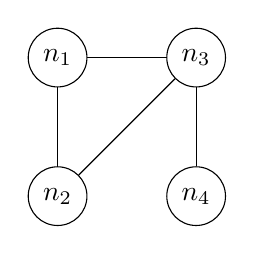
\begin{tikzpicture}
  \node(n1)[circle,draw]{$n_1$};
  \node(n2)[circle,draw,below=of n1]{$n_2$};
  \node(n3)[circle,draw,right=of n1]{$n_3$};
  \node(n4)[circle,draw,right=of n2]{$n_4$};
  \draw(n1)--(n2);
  \draw(n1)--(n3);
  \draw(n2)--(n3);
  \draw(n3)--(n4);
\end{tikzpicture}
\begin{tabular}[b]{lll}
   $\mathfrak{G} = \{\mathfrak{N} ,\mathfrak{A}\}$\\
  $\mathfrak{N}=\{n_1,n_2,n_3,n_4\}$\\
  $\mathfrak{A}=\{\{n_1,n_2\},\{n_1,n_3\},\{n_2,n_3\},\{n_3,n_4\}\}$
\end{tabular}
\begin{tabular}[b]{c|c:c:c:c}
      $\mathfrak{G}$ & $n_1$ & $n_2$ & $n_3$ & $n_4$ \\
\hline
$n_1$ & 0 & 1 & 1 & 0 \\
\hdashline
$n_2$ & 1 & 0 & 1 & 0 \\
\hdashline
$n_3$ & 1 & 1 & 0 & 1 \\
\hdashline
$n_4$ & 0 & 0 & 1 & 0 \\
\end{tabular}
}
\end{figure}

x\syntRel{obl-obj}{}x     x\syntRelLeft{obl-obj}{}x

x\syntRel{posssess}{}x     x\syntRelLeft{posssess}{}x





% \index[notion]{lexical entry}

\maketitle

\frontmatter
\currentpdfbookmark{Contents}{name} % adds a PDF bookmark
{\sloppy\tableofcontents}

\mainmatter
% !TEX root = LF-IMAPol.tex

\ohead{Writing conventions}

\chapter*{Writing conventions}
\addcontentsline{toc}{chapter}{Writing conventions}

\noindent
\begingroup
\setlength{\tabcolsep}{2.5pt}
\setlength\extrarowheight{3pt}
\small
\begin{longtable}{ l l >{\raggedright\arraybackslash}p{10cm} }

\multicolumn{3}{l}{{\large \textbf{Abbreviations}}} \\*[6pt]

$\mathcal{A}$ & \phantom{:} & a set of arcs in a network\slashs{}graph \\

\textsc{acc} & \phantom{:} & accusative case \\

Adj & \phantom{:} & Adjective \\

Adv & \phantom{:} & Adverb \\

A\tsub{(poss)} & \phantom{:} & possessive adjective (\textit{my}, \textit{your}, ...) \\

\textsc{art} & \phantom{:} & article or other determiner -- e.g. \textit{to have} \textsc{art} \textit{dream} \\

Claus & \phantom{:} & Clausative \\

\syntDname{circumst} & \phantom{:} & \syntDname{circumstantial} surface-syntactic relation \\

\textsc{dat} & \phantom{:} & dative case \\

\syntDname{determ} & \phantom{:} & \syntDname{determinative} surface-syntactic relation \\

\syntDname{dir-obj} & \phantom{:} & \syntDname{direct-objectival} surface-syntactic relation \\

DSynt- & \phantom{:} & deep-syntactic \\

DSyntA & \phantom{:} & deep-syntactic actant \\

DSyntS & \phantom{:} & deep-syntactic structure \\

%{\smaller Eng.} & \phantom{:} & English \\

\lf{f} & \phantom{:} & A given lexical function \\

\lfappl{f}{L} & \phantom{:} & Application of the lexical function \lf{f} to its argument (lexical unit)~L \\

%{\smaller Fr.} & \phantom{:} & French \\

fr-LN & \phantom{:} & French Lexical Network \\

$\mathcal{G}$ & \phantom{:} & a given graph \\

$\mathcal{G}_{LS}$ & \phantom{:} & a given Lexical System graph \\

\textsc{gen} & \phantom{:} & genitive case \\

\textsc{ger} & \phantom{:} & gerund \\

\textsc{instr} & \phantom{:} & instrumental case \\

L & \phantom{:} & a given lexical unit, i.e. a lexeme or an idiom \\*

& & \multicolumn{1}{>{\raggedright\arraybackslash}p{10cm}}{\footnotesize \remark{Note.}In the body of the book, we allow ourselves to use the symbol ``L'' in the sense of `referent\index[notion]{referent} of lexical unit L' -- e.g., [...]~\textit{prototypically used to do L} in the description of \lf{S\tsub{instr}} (\chapref{chap:paraLFs}, [\ref{lf:S-instr}], p.\thinspace\pageref{lf:S-instr}).} \\

L\tsub{\textsc{gener}} & \phantom{:} & generic term (of a semantic field) \\

\lang & \phantom{:} & a given natural language \\

%{\smaller Lat.} & \phantom{:} & Latin \\

LF & \phantom{:} & lexical function \\

LN & \phantom{:} & lexical network \\

\textsc{loc} & \phantom{:} & locative case \\

LDOCE & \phantom{:} & \textit{Longman Dictionary of Contemporary English} (online) \\

\syntDname{modif} & \phantom{:} & \syntDname{modificative} surface-syntactic relation \\

\textit{n} & \phantom{:} & a given node in a network\slashs{}graph \\

$\mathcal{N}$ & \phantom{:} & a set of nodes in a network\slashs{}graph \\

N & \phantom{:} & Noun \\

\textsc{nom} & \phantom{:} & nominative case \\

\syntDname{obl-obj} & \phantom{:} & \syntDname{oblique-objectival} surface-syntactic relation \\

\textsc{pl} & \phantom{:} & plural \\

PoS & \phantom{:} & part of speech \\

\syntDname{possess} & \phantom{:} & \syntDname{possessive}  surface-syntactic relation \\

\syntDname{prepos} & \phantom{:} & \syntDname{prepositional} surface-syntactic relation \\

\textsc{prepos} & \phantom{:} & prepositional case \\

%{\smaller Rus.} & \phantom{:} & Russian \\

\lf{S} & \phantom{:} & substantive [= `noun'; in the name of a nominal lexical function] \\

SAE & \phantom{:} & Standard Average European [language type; roughly, Germanic, Romance and Slavic languages] \\

Sem- & \phantom{:} & semantic \\

SemA & \phantom{:} & semantic actant \\

SemS & \phantom{:} & semantic structure \\

\textsc{sg} & \phantom{:} & singular \\

SSyntS & \phantom{:} & surface-syntactic structure \\

\syntDname{subj} & \phantom{:} & \syntDname{subjectival} surface-syntactic relation \\

\syntDname{subj-adnom} & \phantom{:} & \syntDname{subjectival-adnominal} surface-syntactic relation \\

V & \phantom{:} & Verb \\[-12pt]

\end{longtable}
\endgroup

\noindent
\begingroup
\setlength{\tabcolsep}{2pt}
\setlength\extrarowheight{3pt}
\small
\begin{longtable}{ l l >{\raggedright\arraybackslash}p{9.1cm} }

\multicolumn{3}{l}{{\large \textbf{Symbols}}} \\*[6pt]

*A & \phantom{:} & A is ungrammatical \\

A\enskip≈\enskip A & \phantom{:} & A and B are approximately equal; in the present volume, the symbol ``≈'' mostly stands for \textit{approximately} \\

A\enskip{\footnotesize $\equiv$}\enskip B & \phantom{:} & A and B are equivalent \\

A\enskip{\footnotesize $\cong$}\enskip B & \phantom{:} & A and B are approximately equivalent \\

\textbf{s\tsub{1}} $\oplus$ \textbf{s\tsub{2}} & \phantom{:} & linguistic union of (components of) linguistic signs \textbf{s\tsub{1}} and \textbf{s\tsub{2}} \\

E\thinspace\constrbar\thinspace C & \phantom{:} & constraint C on the expression E -- e.g., \lfappl{Loc\tsub{in}}{\textit{weather}} = \newline\textit{in} \lfgp{\tld\ \constrbar\ with a modifier} (i.e., one says \textit{in this}\slashs\textit{such weather}, \textit{in rainy weather}, \textit{in weather like this}, etc.) \\

E\tsub{1} $\langle$E\tsub{2}$\rangle$ & \phantom{:} & expression E\tsub{2} is a variant of expression E\tsub{1} \\

A\thinspace$\Rightarrow$\thinspace{}B & \phantom{:} & A implies B \\

A\thinspace$\Leftrightarrow$\thinspace{}B & \phantom{:} & linguistic entity A of the level $n$ of representation corresponds [=~is semantically equivalent] to linguistic entity B of level $n+1$, and vice versa; for instance:\vspace{-3pt} \\*
&&\hphantom{ii}`Joey\thinspace\syntRelLeft{1}\thinspace\myuline{sleep}' \lfgp{SemS} $\Leftrightarrow$ \textsc{Joey}\thinspace\syntRelLeft{I}\thinspace\textsc{sleep}\tsub{(V)} \lfgp{DSyntS}. \\

\lf{f\tsub{$\supset$}}, \lf{f\tsub{$\subset$}}, \lf{f\tsub{$\cap$}} & \phantom{:} & lexical function that is semantically richer ({\scriptsize $\supset$}) or poorer ({\scriptsize $\subset$}) than \lf{f}, or has semantic intersection ({\scriptsize $\cap$}) with \lf{f} \\

\raisebox{-.6ex}{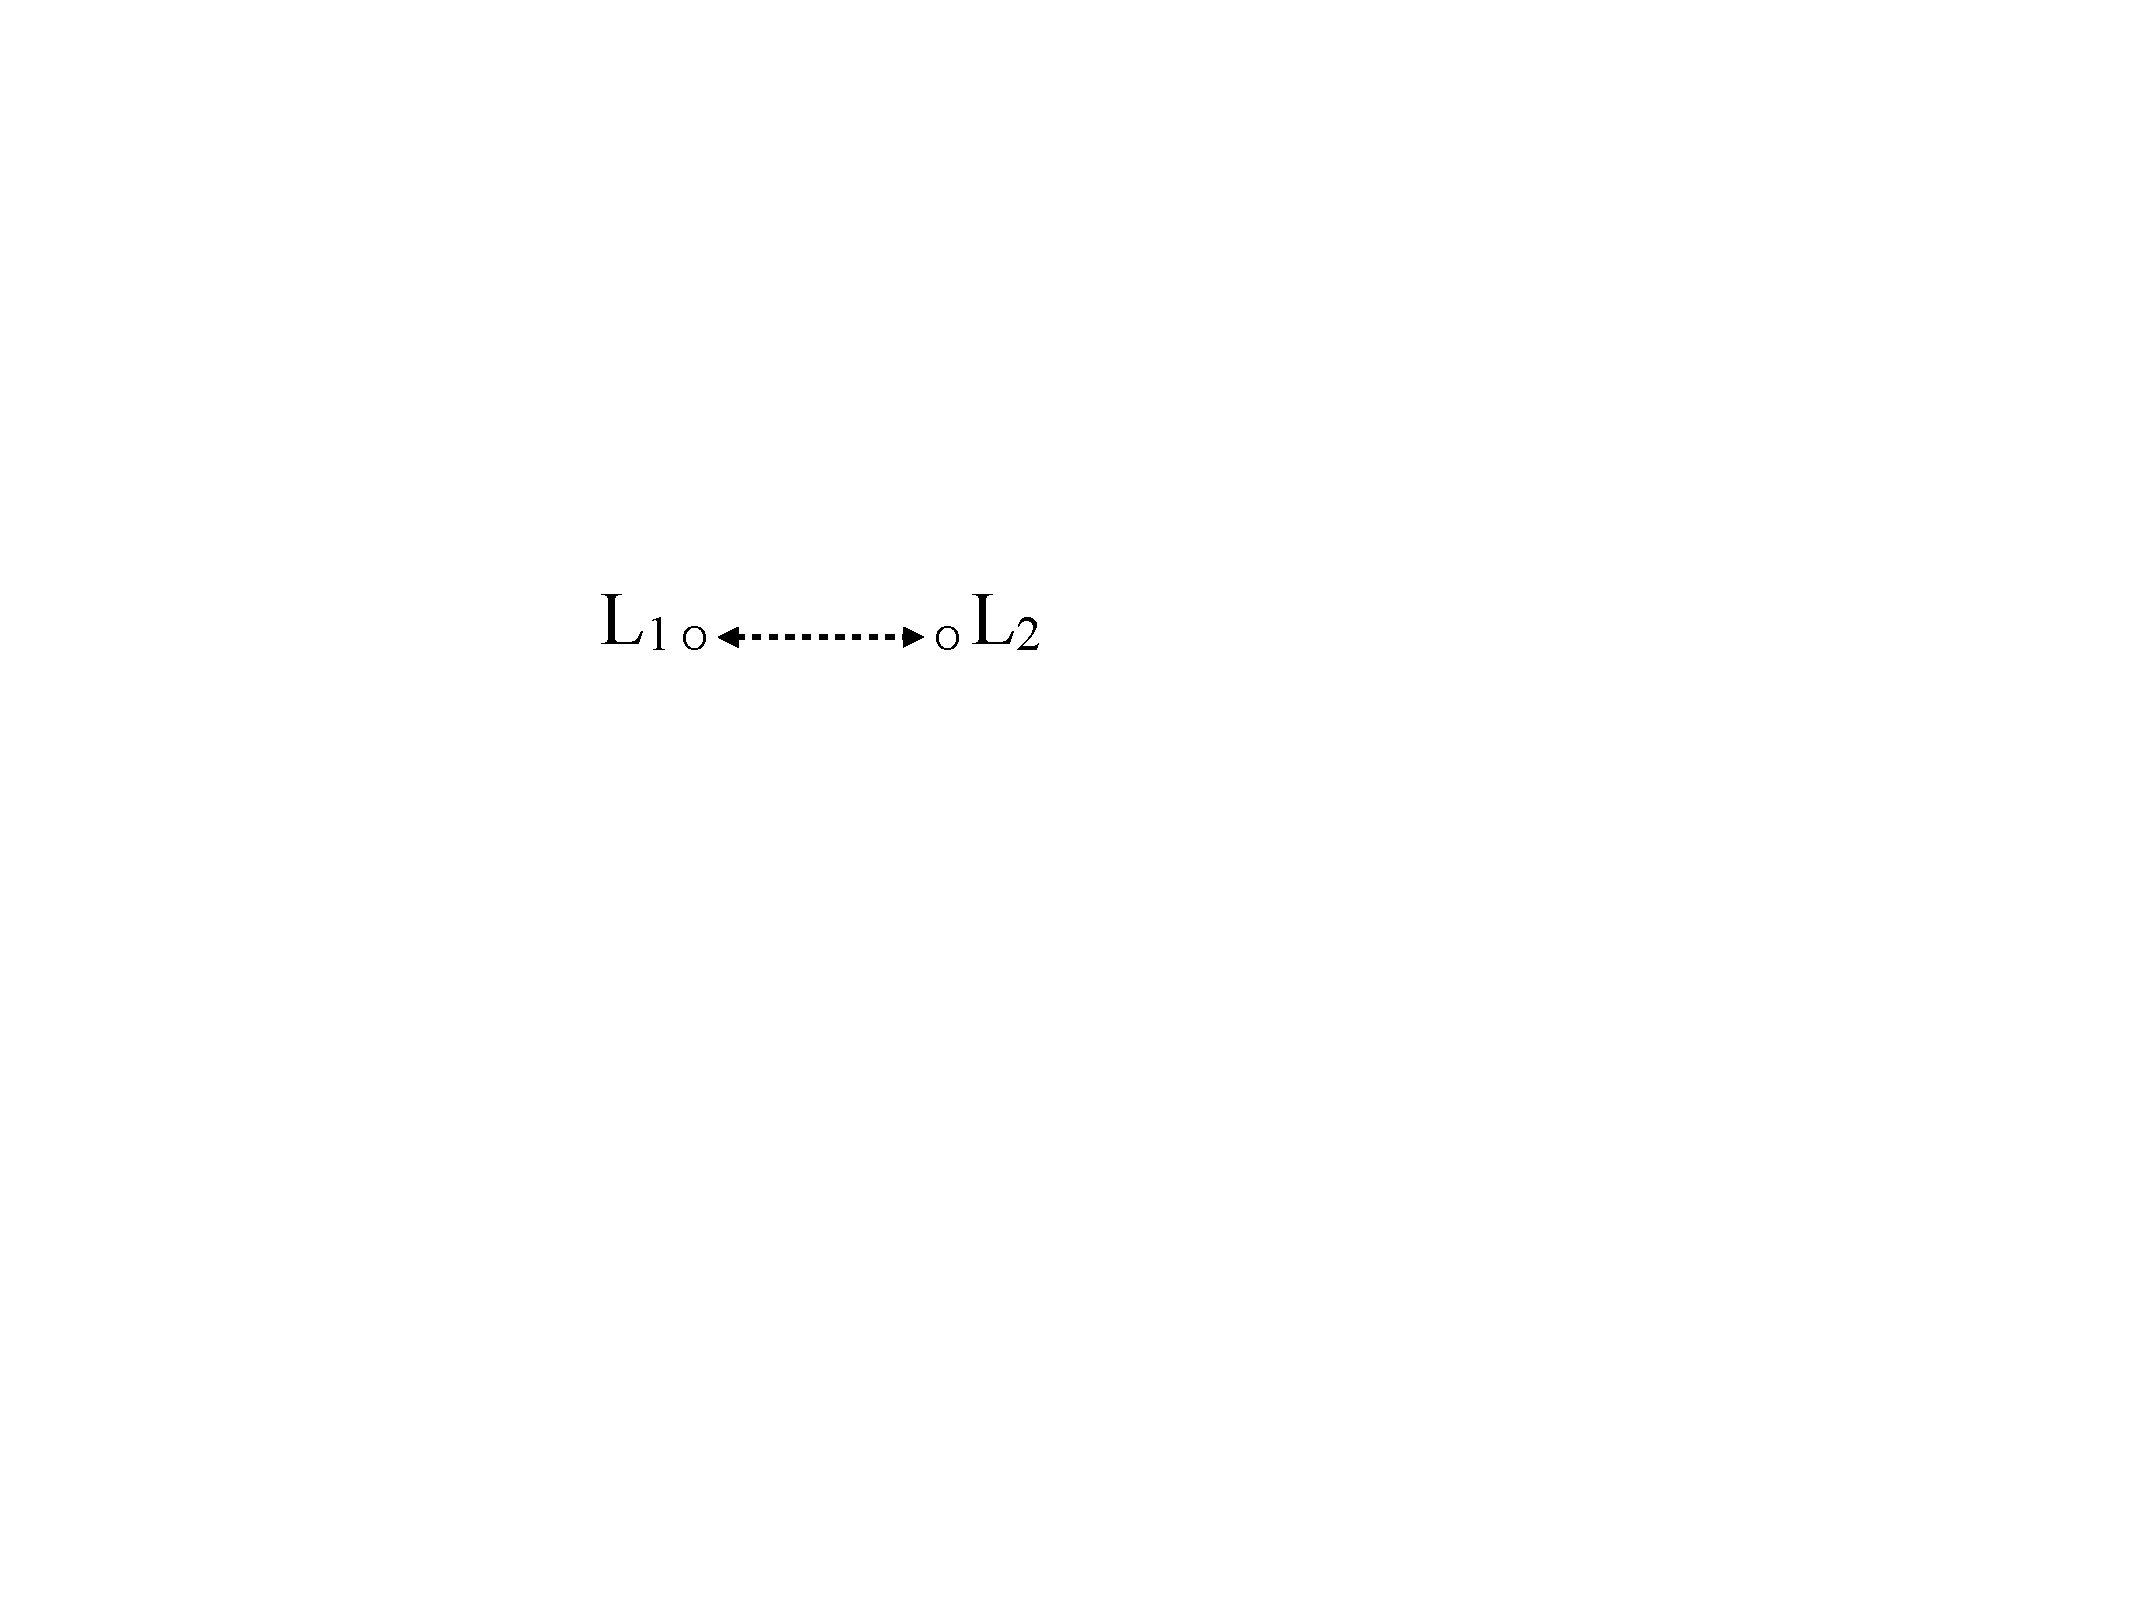
\includegraphics[width=2.2cm]{Fig/SymbAbbrev/CorefNodes.pdf}} & \phantom{:} & in a syntactic representation, indicates that the nodes L\tsub{1} and L\tsub{2} are coreferential -- i.e., they have the same referent \\

L\tsub{1}\thinspace\syntRel{Dep}\thinspace{}L\tsub{2} & \phantom{:} & L\tsub{2} semantically\slashs{}syntactically depends on L\tsub{1} by semantic\slashs{}syntactic dependency \textbf{\textsf{Dep}} \\

L\thinspace\lexRel{\lf{LexRel}}\thinspace{}L′ & \phantom{:} & L′ is the target of the  lexical relation \lf{LexRel} originating from L \\

\idiom{L\tsub{1} ... L\tsub{n}} & \phantom{:} & idiom -- e.g., \idiom{\textit{put the cart before the horse}} \\

\tld & \phantom{:} & the lexical unit under description in a given formula -- e.g., \lfappl{Real\tsub{1}}{\textit{bicycle}} = \textit{ride} \lfgp{\textsc{art} \tld} \\

\suffixsplit & \phantom{:} & \lfgp{in a Russian wordform} boundary between a morphological stem and a suffix\index[notion]{suffix} -- e.g., \textit{sobak\suffixsplit{}a} `dog-\textsc{sg.nom}' \\

\onewdf & \phantom{:} & graphical connector for segments of one wordform that is traditionally spelled as several words -- e.g. \textit{at\onewdf{}last} \\

`\textsigma' & \phantom{:} & a given meaning \\

\sigmaF\ & \phantom{:} & meaning of the lexical function \lf{f} \\

`\myuline{\textsigma}' & \phantom{:} & semanteme that is communicatively dominant in a semantic structure \\

`\tsub{---}' & \phantom{:} & empty actant slot in a semantic structure \\

\textOmega & \phantom{:} & external participant of the situation denoted by L (i.e., a participant that is not expressed as one of L's semantic actants) \\

Ø & \phantom{:} & zero sign \\[2pt]

\multicolumn{3}{l}{In the list of an LF application values (\textit{Val}):} \\*


\textit{Val\tsub{1}}\textbf{;} \textit{Val\tsub{2}} &  & there is a notable semantic difference between \textit{Val\tsub{1}} and \textit{Val\tsub{2}} \\

\textit{Val\tsub{1}} \textbf{<} \textit{Val\tsub{2}} &  & \textit{Val\tsub{2}} is semantically `more' than \textit{Val\tsub{1}}; the left and right scopes of ``<'' can be limited by the ``;'' symbol \\

\fused\textit{Val} &  & \textit{Val} is a fused value element (for a syntagmatic LF) \\*

\textit{Val} \lfgp{GP} & & GP is the government pattern of \textit{Val} -- e.g., \lfappl{Oper\tsub{1}}{\textit{supremacy}} = \textit{detain} \lfgp{\textsc{art} \tld} \\ [-12pt]

\end{longtable}
\endgroup

\noindent
\begingroup
\setlength{\tabcolsep}{2.5pt}
\setlength\extrarowheight{3pt}
\small
\begin{longtable}{ l l >{\raggedright\arraybackslash}p{9cm} }

\multicolumn{3}{l}{{\large \textbf{Special font formats}}} \\*[6pt]

\textsc{small capitals} & \phantom{:} &  lexical unit supplied, when needed, with its lexicographic number -- e.g., the lexeme \textsc{step}\tsub{(V)}\sensenum{I.1} and the idiom \idiom{\textsc{blow the whistle}} \\

\lf{monospace font} & \phantom{:} & lexical function's name -- e.g., \lf{Syn}, \lf{A\tsub{1}}, ... \\

\notion{italicized sans serif font} & \phantom{:} & important notion, when first introduced -- e.g., \notion{idiom} \\*

\uslabel{small bold sans serif font} & \phantom{:} & usage label -- e.g., \uslabel{archaic}, \uslabel{child language}, \uslabel{colloquial}, ...
% Label labels used in the book
% archaic
% child language
% colloquial
% dated
% formal
% informal
% literary
% offensive
% Quebec
% slang
% specialized
% vulgar

\end{longtable}
\endgroup

\noindent
Russian examples are in international scientific transliteration\index[notion]{transliteration}; it is as follows:

\begin{center}
\small
\noindent
\renewcommand*{\arraystretch}{1.2}
\setlength{\tabcolsep}{1.5pt}
\begin{tabular}{ l c l c l c l c l c l c l c l c l c l c l c l }
\midrule

Aa &---& Аа
&\phantom{.....}& Ëë &---& Ёё
&\phantom{.....}& Ja ja &---& Яя
&\phantom{.....}& Oo &---& Оо
&\phantom{.....}& Tt &---& Тт
&\phantom{.....}& \v{Z}\v{z} &---& Жж \\

Bb &---& Бб
& & Èè &---& Ээ
& & Ju ju &---& Юю
& & Pp &---& Пп
& & Uu &---& Уу
& & \palat\ &---& Ьь \\

Cc &---& Цц
& & Ff &---& Фф
& & Kk &---& Кк
& & Rr &---& Рр
& & Vv &---& Вв
& & \palat\palat\ &---& Ъъ \\

\v{C}\v{c} &---& Чч
& & Gg &---& Гг
& & Ll &---& Лл
& & Ss &---& Сс
& & Xx &---& Хх
& & & & \\

Dd &---& Дд
& & Ii &---& Ии
& & Mm &---& Мм
& & \v{S}\v{s} &---& Шш
& & Yy &---& Ыы
& & & & \\

Ee &---& Ее
& & Jj &---& Йй
& & Nn &---& Нн
& & \v{S}\v{c}, \v{s}\v{c} &---& Щщ
& & Zz &---& Зз
& & & & \\

\midrule
\end{tabular}
\end{center}

\clearpage{\pagestyle{empty}\cleardoublepage}


\include{chapters/02-LFlist}
\include{3-Forewords}
% !TEX root = LF-IMAPol.tex

\chapter{Introduction}\label{chap:Introduction}

\section{Our object of study: lexical functions}\label{sec:aboutWhat}

This book is about \notion{lexical functions}\index[notion]{lexical function}. Therefore, our very first task is to explain -- at least, approximately, in simple terms and with the help of most trivial examples -- what lexical functions are. Let's do it!

Consider the phrases in \Next and \NNext:\footnote{As is customary, we use the asterisk ``*'' in front of an expression to indicate that this expression is ungrammatical. Let it be emphasized that for an expression to be ungrammatical does not imply that it cannot be found in speech. For instance, at the time of writing, the one-billion-word Corpus of Contemporary American English \parencite{Davies2008} contained 1,676 occurrences of \textit{pay tribute} and 13 occurrences of the ungrammatical phrase *\textit{give tribute} (for all inflected forms of these phrases). Additionally, the acceptability of word combinations can fluctuate significantly due to geographical variation. We are grateful to Alastair Butler for the suggestion to use \ref{ex:payTribute} and \ref{ex:giveRecognition} as illustrations.}\index[notion]{ungrammaticality}\index[notion]{COCA corpus}

\begingroup
\small

\ex.\label{ex:payTribute} \a. \emph{pay} tribute \lfgp{to someone}
     \b. *\emph{give} tribute \lfgp{to someone}

\ex.\label{ex:giveRecognition} \a. \emph{give} recognition \lfgp{to someone}
     \b. *\emph{pay} recognition \lfgp{to someone}\hspace{25pt}

\endgroup

The verbs \textit{pay} and \textit{give}, used in \LLast[a] and \Last[a] with the nouns \textit{tribute} and \textit{recognition}, respec­tively, are not interchangeable in spite of the following facts:

\begin{itemize}

\item The two nouns are semantically close.

\item The two verbs are, so to speak, pure verbalizers\index[notion]{verbalizer} of their nominal objects: they express a very general, impoverished meaning, approximately `do', and add no semantic content to the nouns.

\end{itemize}

These verbs are empty of meaning in the given contexts to such an extent that \textit{pay tribute} is semantically reducible to a hypothetical verb *\textit{to tribute} \lfgp{\textit{someone}}, and \textit{give recognition}, to the verb \textit{to recognize} \lfgp{\textit{someone} (\textit{during a ceremony})}. For this reason, verbs such as \textit{pay} and \textit{give} are called \emph{support}, or \emph{light}, verbs\index[notion]{support verb}\index[notion]{verb!support \tld} (see \chapref{chap:syntLFs}, \sectref{sec:verbeSupport}).

The choice of the appropriate support verb by the Speaker\index[notion]{Speaker, the} is, as one sees in \ref{ex:payTribute} and \ref{ex:giveRecognition}, contingent upon a specific nomin­al lexeme -- the direct object of this verb: the meaning `do' is ex­pressed by the verb \textit{pay} if you `do' \textit{tribute}, but by the verb \textit{give} if you `do' \textit{recognition}. In other words, the meaning `do' is expressed not freely\index[notion]{meaning!free \tld}, that is, not by any convenient verb the Speaker is able to think of. It is expressed in a constrained way\index[notion]{meaning!constrained \tld}: by the verb that the noun imposes. To borrow from the language of mathematics\index[notion]{mathematical function}, the meaning `do' is expressed \emph{as function of} the direct object of the corresponding verb. This is where the noun \textit{function} in the term \textit{lexical function} comes from. The reason for the adjective \textit{lexical} is obvious: such functions apply to lexical units\index[notion]{lexical unit} and return lexical entities\index[notion]{lexical entity} -- on the notion of lexical entity, see \sectref{sec:lexicalNotions} (p.\thinspace\pageref{def:lexicalEntity}).

\begin{soundbox}{Syntagmatic lexical function}
What is illustrated in \ref{ex:payTribute} and \ref{ex:giveRecognition} is a \emph{syntagmatic} lexical function\index[notion]{lexical function!syntagmatic \tld}\index[notion]{syntagmatic!\tld\ lexical function} called \lf{Oper\tsub{1}}\index[lf]{Operi@\lf{Oper\tsub{i}}!\lf{Oper\tsub{1}}} (see \chapref{chap:syntLFs}, [\ref{lf:Oper-i}], p.\thinspace\pageref{lf:Oper-i}), which describes a particular pattern of constrained lexical unit combinations -- that is, a particular type of a two-component phrase where one lexical unit, freely selected by the Speaker, determines the selection of the other lexical unit. In this specific case, borrowing again from mathematical formalization, we write:

\phantom{.}
\begingroup
\small

\ex.[] \setlength{\tabcolsep}{2pt}\begin{tabular}[t]{ l c >{\raggedright\arraybackslash}p{6cm} }
\lfappl{Oper\tsub{1}}{\textit{tribute}} & = & \textit{pay} \lfgp{\textit{tribute}} \\
\lfappl{Oper\tsub{1}}{\textit{recognition}} & = & \textit{give} \lfgp{\textit{recognition}} \\
\end{tabular}

\endgroup

Constrained lexical combinations described by syntagmatic lexical functions are termed \emph{collocations} (see \chapref{chap:NotionLF}, \sectref{sec:classeFLSyntagmatiques}). They are extremely varied -- support-verb constructions (presented above), realization-verb constructions (\textit{pay a debt}, \textit{satisfy a desire}, \textit{ring a bell}), \mbox{(de-)intensifying} modifier constructions (\textit{generous}\slashs\textit{meager salary}, \textit{remember clearly}\slashs\textit{vaguely}), etc. -- and their description requires a wide range of syntagmatic lexical functions.
\end{soundbox}

\largerpage[-1]
Lexical functions are not limited to constrained combinations of \emph{lexical units} within \emph{phrases}: they similarly deal with constrained combinations of \emph{morphemes}\index[notion]{morpheme} within \emph{wordforms}\index[notion]{wordform}. For instance, in English, the derivational means\index[notion]{derivative!morphological \tld} used to produce from a verb V the noun that means `person who does V' is contingent upon V, as illustrated in \Next:

\begingroup
\small
 
 \ex.\label{ex:S1Derivations} \begingroup\setlength{\tabcolsep}{2pt}
\begin{tabular}[t]{ l c l c >{\raggedright\arraybackslash}p{5cm} }
\textit{teach} & $\Rightarrow$ & \textit{teacher} & : & \textbf{-er} suffixation \\
\textit{represent} \lfgp{\textit{a social group}} & $\Rightarrow$ & \textit{representative}\tsub{(N)} & : & \textbf{-(at)ive} suffixation \\
\textit{chair}\tsub{(V)} \lfgp{\textit{a meeting}} & $\Rightarrow$ & \textit{chairperson} & : & compounding \\
\textit{guide}\tsub{(V)} & $\Rightarrow$ & \textit{guide}\tsub{(N)} & : & V\thinspace$\Rightarrow$\thinspace{}N conversion \\
\textit{steal}\tsub{(V)} & $\Rightarrow$ & \textit{thief} & : & suppletive form \\
\end{tabular}\endgroup

\endgroup\index[notion]{suffixation}\index[notion]{compounding}\index[notion]{conversion, morphological}\index[notion]{suppletion}

In parallel with what has been said about the meaning `do' for our first set of illustrations, we say that the meaning `person who does [V]' is expressed as function of the verb V in order to return the corresponding noun.

\begin{soundbox}{Paradigmatic lexical function}
The constrained combinations of morphemes\index[notion]{morpheme} illustrated in \ref{ex:S1Derivations} are also representable by means of a lexical function; in this case, a \emph{paradigmatic} lexical function\index[notion]{lexical function!paradigmatic \tld}\index[notion]{paradigmatic!\tld\ lexical function} called \lf{S\tsub{1}}\index[lf]{Si@\lf{S\tsub{i}}!\lf{S\tsub{1}}} (see \chapref{chap:paraLFs}, [\ref{lf:S-i}], p.\thinspace\pageref{lf:S-i}). Accordingly, we write:

\phantom{.}
\begingroup
\small

\ex.[] \setlength{\tabcolsep}{2pt}\begin{tabular}[t]{ l c >{\raggedright\arraybackslash}p{8cm} }
\lfappl{S\tsub{1}}{\textit{teach}} & = & \textit{teacher} \\
\lfappl{S\tsub{1}}{\textit{represent}} & = & \textit{representative}\tsub{(N)} \\
\lfappl{S\tsub{1}}{\textit{chair}\tsub{(V)}} & = & \textit{chairperson} \\
\lfappl{S\tsub{1}}{\textit{guide}\tsub{(V)}} & = & \textit{guide}\tsub{(N)} \\
\lfappl{S\tsub{1}}{\textit{steal}\tsub{(V)}} & = & \textit{thief} \\
\end{tabular}

\endgroup

\noindent
\remark{Notation.}As can be seen, we indicate in subscript the part of speech of a lexical unit if it has a homonym of a different part of speech.
\end{soundbox}

Summing up, lexical functions are a formal tool designed to describe specific patterns of constrained combinations of linguistic signs\index[notion]{linguistic sign} -- of lexical units as well as of morphemes\index[notion]{morpheme}.\footnote{The morphemes in question are mostly derivational morphemes, that is, morphemes whose meanings are fairly close to lexical meanings.} As such, lexical functions account for an important part of natural languages' phraseology\index[notion]{phraseology}:\footnote{On the notions of phraseme and phraseology, see \sectref{sec:lexicalNotions}, p.\thinspace\pageref{sec:lexicalNotions}.} lexical as well as morphological phraseology\index[notion]{phraseology!lexical \tld}\index[notion]{phraseology!morphological \tld} \parencite{Melcuk2021b}.\phantomsection\label{txt:LFsAndPhraseology}

The set of lexical functions is organized around a rigorously structured system of \emph{simple standard} lexical functions\index[notion]{lexical function!standard \tld}\index[notion]{system of standard LFs}\index[notion]{lexical function!system of standard \tlds}, whose number is under 70 (see \chapref{chap:NotionLF}, p.\thinspace\pageref{tab:systFL}). One of their defining properties is that they are language-universal\index[notion]{universal|see{language-universal}}\index[notion]{language-universal} (see \sectref{sec:FLStandard2Carac}, p.\thinspace\pageref{sec:universality}).

\begin{soundboxnotitle}
To avoid misunderstanding, let us stress that lexical functions are by no means semantic units -- a kind of elementary meanings. They do not exist on the semantic level of linguistic represen­tation. They are special -- namely, deep -- lexical units\index[notion]{lexical unit!deep \tld}, appearing in the deep-syntactic structures of utterances and participating in deep-syntactic paraphrasing\index[notion]{paraphrase!syntactic \tld} (see \sectref{sec:DSyntAndLFs}, p.\thinspace\pageref{sec:DSyntAndLFs}).\footnotemark\ One can say that a lexical function is, metaphorically speaking, a lexical unit ``of the second order.'' Like any lexical unit, it possesses a signified\index[notion]{signified}, a signifier\index[notion]{signifier} and a syntactics\index[notion]{syntactics} -- a set of combinatorial properties; the remarkable fact is that a lexical function's signifier is a set of alternating lexical expressions. On the syntactics -- third component of a linguistic sign, see \textcite{Melcuk2013a}.\index[notion]{linguistic sign}
\end{soundboxnotitle}\footnotetext{Recall the equivalence mentioned above: \textit{give}\tsub{\lfappl{Oper$_\text{1}$}{\textit{recognition}}} \textit{recognition}{\enskip\scriptsize $\equiv$\enskip}\textit{recognize}.}

\textit{Lexical Functions: The Naked Truth} presents the system of lexical functions as fully as possible, but with the following two restrictions.

First, our approach is exclusively synchronic\index[notion]{synchrony}, which means that we avoid the diachronic\index[notion]{diachrony} perspective on word formation or collocations \parencite[cf.][]{Blanco2018-e}, as well as the micro-diachronic study of lexical dynamics\index[notion]{lexical dynamics}, such as the transformation of idioms into collocations \parencite[cf.][]{PausePolguere2020-e,PolguereToAppear}.

Second, our presentation is restricted to theoretical and descriptive considerations and we do not touch on domains of practical applications of lexical functions such as:

\begin{itemize}

\item pedagogical applications, that is, language teaching and learning\index[notion]{teaching\slashs{}learning, language}\index[notion]{language teaching\slashs{}learning};

\item psycholinguistics\index[notion]{psycholinguistics}, that is, Mental Lexicon\index[notion]{Mental Lexicon}\index[notion]{lexicon!Mental Lexicon} issues such as language acquisition\index[notion]{acquisition!language \tld}, access to and loss of lexical knowledge\index[notion]{lexical knowledge};

\item Natural Language Processing\index[notion]{Natural Language Processing} -- e.g., extraction\slashs{}interpretation of phraseological expressions\index[notion]{phraseology}, training of Language Models for Artificial Intelligence\index[notion]{Artificial Intelligence}, etc.

\end{itemize}

However,\phantomsection\label{txt:lexicographicApplications} one essential application of lexical functions is systematically taken into consideration throughout the book: it is the lexicographic\index[notion]{lexicography} modeling of systems of lexical units, performed according to the theoretical and descriptive principles of Explanatory Combinatorial Lexicology\index[notion]{Explanatory Combinatorial!\tld\ Lexicology}\index[notion]{lexicology!Explanatory Combinatorial \tld} \parencites{Melcuketal1995-e}[Ch.~11]{Melcuk2013c-e}. This includes dictionary models of the lexicon\index[notion]{lexicon!\tld\ model}\index[notion]{model!lexicon \tld}, such as Explanatory Combinatorial Dictionaries\index[notion]{Explanatory Combinatorial!\tld\ Dictionary}\index[notion]{dictionary!Explanatory Combinatorial \tld} \parencite{MelcukZholkovsky1984,MelcukZolkovskij2016,MelcukEtAl1984,MelcukEtAl1988,MelcukEtAl1992,MelcukEtAl1999}, lexical databases\index[notion]{lexical database} \parencite{Polguere2000b,AlonsoRamosEtAl2010,BarriosRodriguezBoguslavsky2019}, as well as lexical network\index[notion]{lexical network}\index[notion]{network \lfgp{see also \textit{graph}}!lexical \tld} models, such as Lexical Systems\index[notion]{Lexical System} \parencite{Polguere2014c-e}.

\section{Our aims}

Lexical functions -- which are hypothesized as being language-universal\index[notion]{language-universal} -- operate at the core of the structuring and functioning of natural languages: organization of lexical knowledge\index[notion]{lexical knowledge}, lexical access\slashs selection\index[notion]{lexical access\slashs{}selection}, paraphrasing\index[notion]{paraphrase}, etc. It is thus important for the notion of lexical function to be understood by as many people as possible, inside and outside the field of linguistic research. However, the hard fact is that lexical functions are familiar to only a limited circle of ``insiders'' and, when used, they are often characterized in a simplistic way, which makes these characterizations mostly ineffective. This may be the result of a certain lack of pedagogy and attractiveness of texts presenting lexical functions. Yet the core cause of this state of affairs is the fact that the notion of lexical function is inherently difficult to assimilate, for at least two reasons.

First, the mastering of lexical functions requires the mastering of a rather rich set of underlying linguistic notions, which are relevant to all structural modules of natural languages. They pertain to semantics, syntax and morphology, that is, to the lexicon\index[notion]{lexicon!\tld\ vs. grammar} as well as to the grammar\index[notion]{grammar!lexicon vs. \tld} of natural languages. For instance, it is impossible to master the above-mentioned syntagmatic lexical function \lf{Oper\tsub{1}}\index[lf]{Operi@\lf{Oper\tsub{i}}!\lf{Oper\tsub{1}}} without mastering Meaning-Text use of (dependency) syntax\index[notion]{dependency!\tld\ syntax}\index[notion]{syntax!dependency \tld}, the distinction between semantic\index[notion]{actant!semantic \tld\ [SemA]}\index[notion]{semantic!\tld\ actant [SemA]} and deep-syntactic\index[notion]{actant!deep-syntactic \tld\ [DSyntA]}\index[notion]{deep-syntactic!\tld\ actant [DSyntA]} actants and, of course, the principles of lexicographic definition\index[notion]{definition!lexicographic \tld}. In other words, to really \emph{understand} lexical functions, one needs to have a bird's-eye view of the organization of natural languages and  not focus solely on specific linguistic modules one happens to have a specific interest in. Lexical functions are fully embedded in the Meaning-Text approach\index[notion]{Meaning-Text!\tld\ approach} to language studies  \parencites{Melcuk1981a,Melcuk2016a,Kahane2003,Milicevic2006} and have to be acquired as such. \figref{fig:MTTModules} visualizes the architecture of a Meaning-Text model\index[notion]{Meaning-Text!\tld\ model} of natural languages: levels of utterance representation and linguistic modules that establish correspondences ($\Leftrightarrow$) between those levels. Though correspondences are bidirectional, this figure has to be read from bottom to top -- according to the Speaker's\index[notion]{Speaker, the} perspective, i.e., in the perspective of speech production\index[notion]{speech!\tld\ production}.

\noindent
\begin{figure}

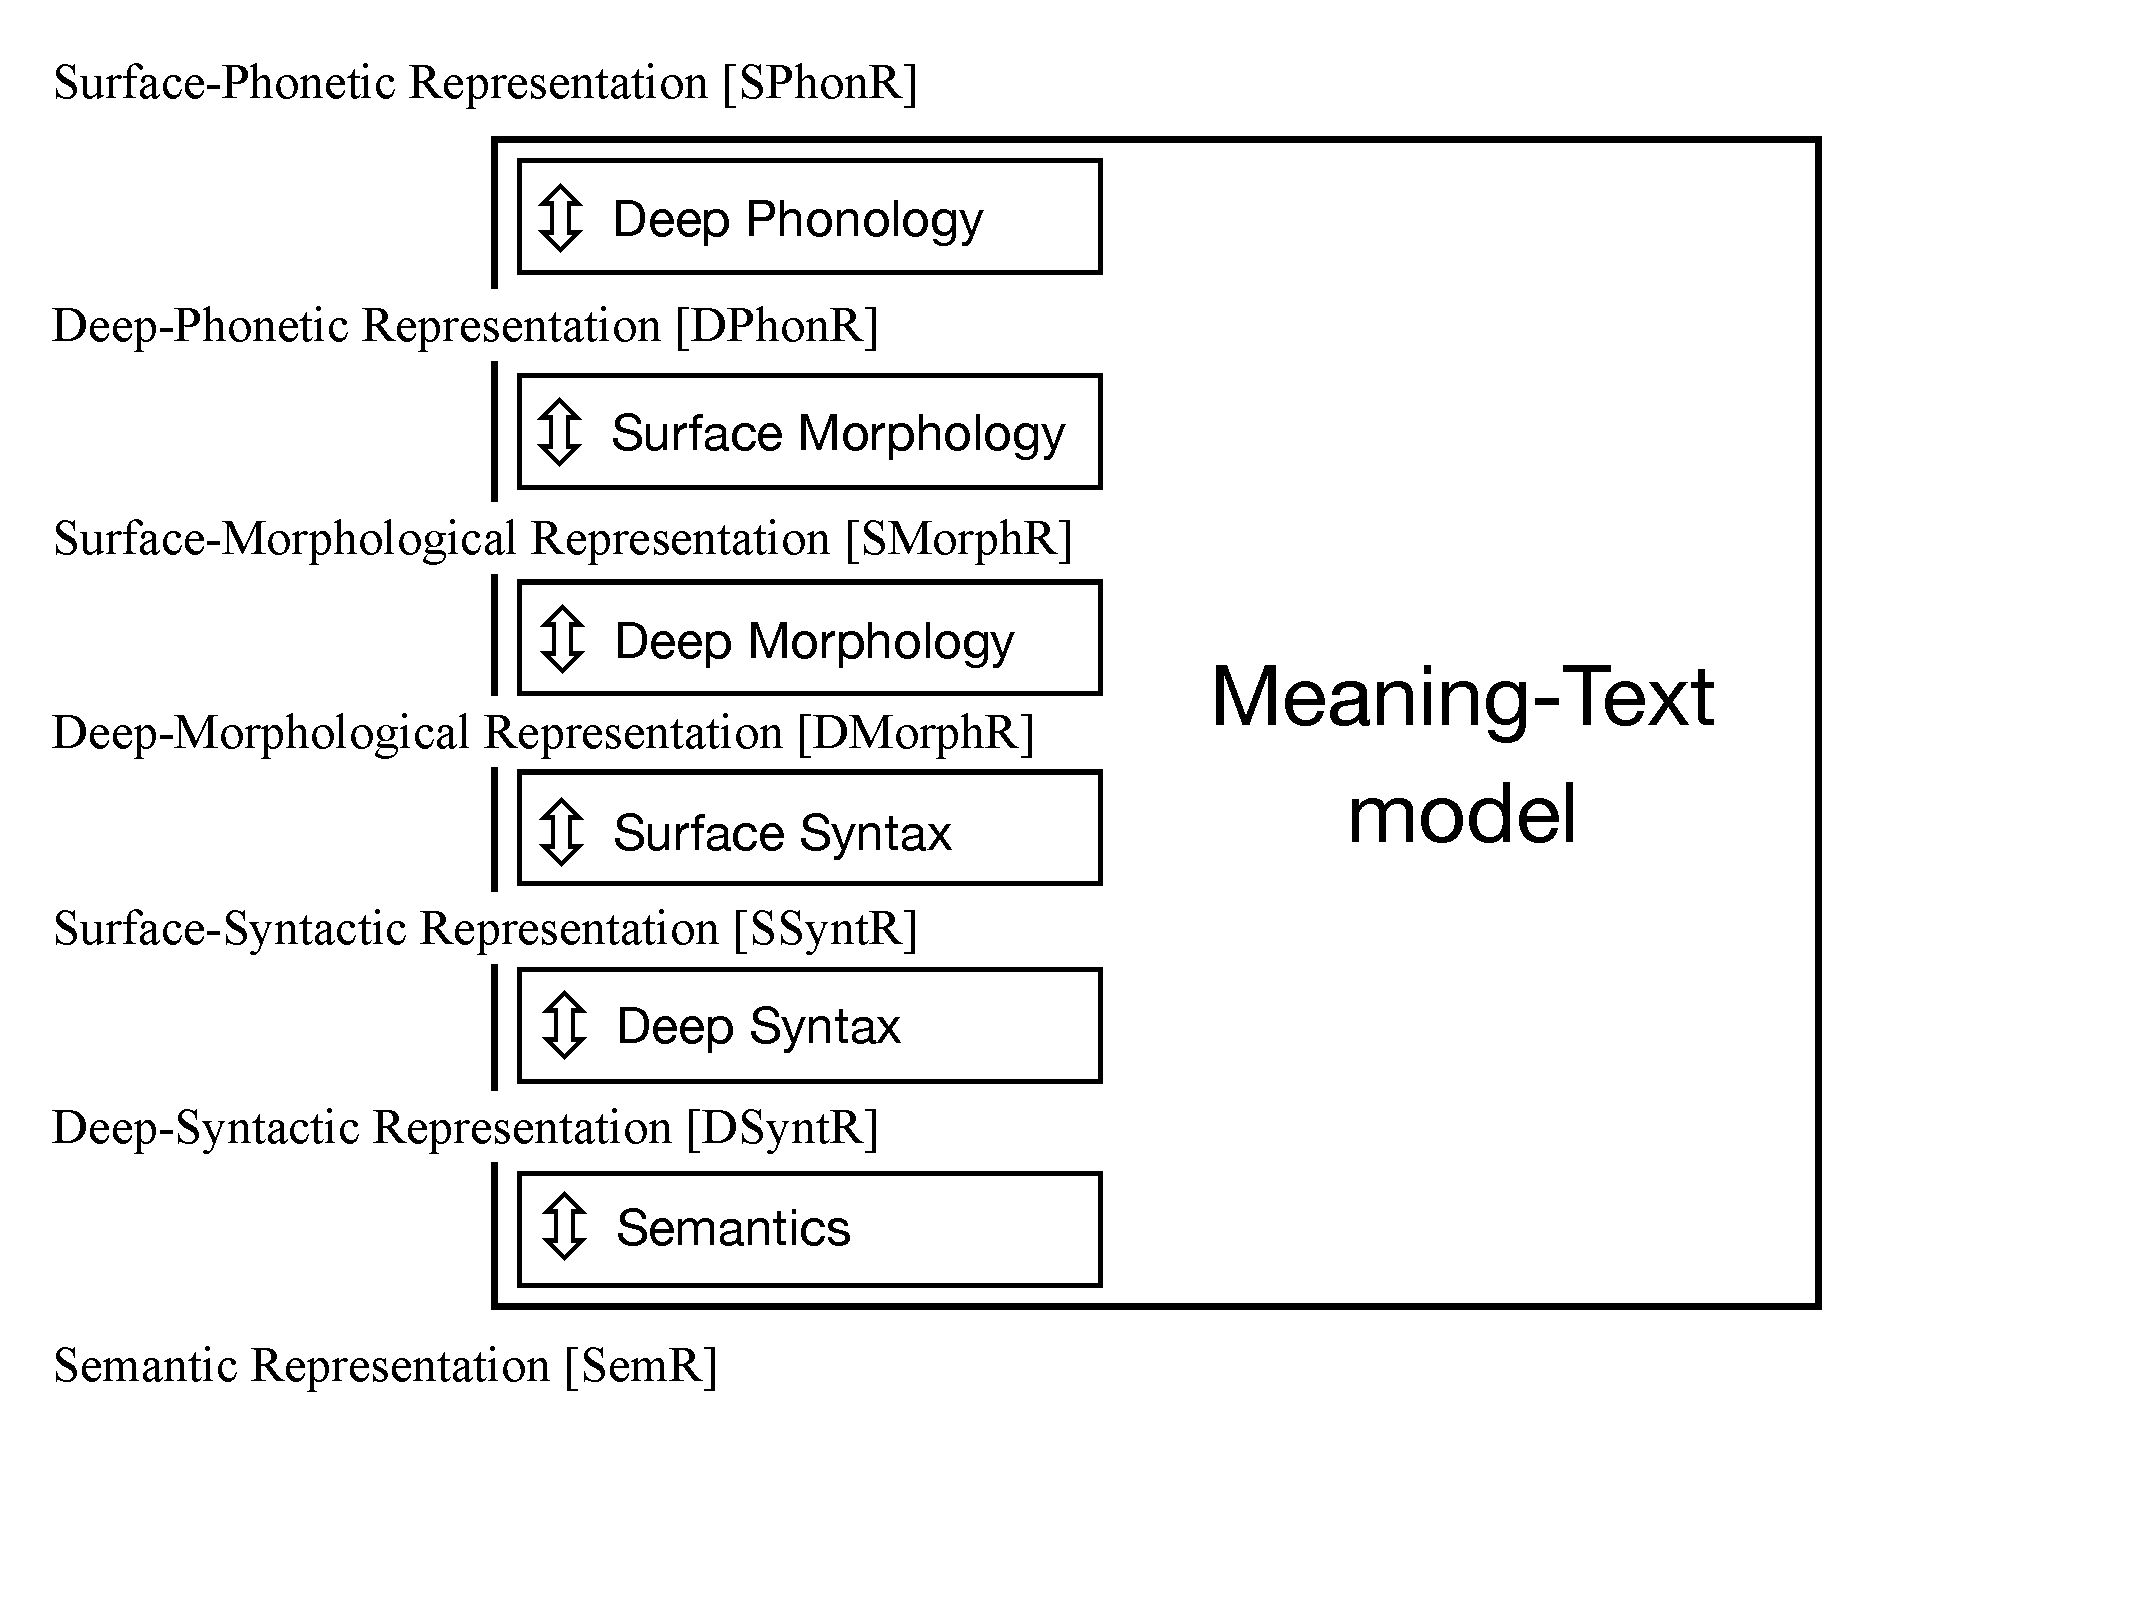
\includegraphics[width=0.8\linewidth]{Fig/Introduction/architectureMTM.pdf}
\caption{Architecture of a Meaning-Text model}\label{fig:MTTModules}
\end{figure}

Second, we have to acknowledge that the formal language of lexical functions\index[notion]{lexical function!formal language of \tlds} is far from being streamlined and self-evident. It tries to reconcile two mutually incompatible imperatives: on the one hand, formal precision; on the other hand, legibility by humans and the possibility of easily applying the researcher's linguistic intuition when reasoning on lexical function formulas. Consequently, the language of lexical functions is sometimes making use of unusual formal conventions -- for instance, the use of actantial subscripts\index[notion]{actantial subscript} (to the names of lexical functions) with different interpretations depending on the context, which is not acceptable in a genuine formal language (\chapref{chap:NotionLF}, Sections~\ref{sec:actSubsSimpleLF} and \ref{sec:actSubsLFCombinations}).\footnote{For an alternative (so-called \textit{algebraic}) notation of lexical functions, see \textcite{KahanePolguere2001-e}. Note that what is gained with this notation in terms of formal rigor and calculability is counterbalanced by a clear loss in terms of possible recourse to linguistic intuition when a lexicographer, a linguist, etc., wants to reason using lexical functions.}

Faced with these difficulties, we decided to deal with the situation frontally, without cutting corners. However, because our ambition is, first of all, to be as much pedagogical as possible, we made a systematic effort at providing readers with all background and, even, insider knowledge needed to achieve an in-depth understanding of lexical functions. We hope therefore that the book can prove useful to a vast range of readers: linguists, lexicographers, researchers and developers in Natural Language Processing, language teachers, translators, etc. -- in a nutshell, to everyone who deals with or is interested in Language.

\section{How do we describe lexical functions?}\label{sec:howDoWeDescribeLFs}

As we just said, this book is intended as a fresh, more pedagogical presentation of the system of lexical functions, which has already been the topic of many publications -- e.g., \textcite{AlonsoRamos1993}, \textcite{Melcuk1996}, \textcite{Melcuk2007b}, \textcite[210--223]{MelcukMilicevic2014a}, \textcite[Ch.~14]{Melcuk2015a-e}, etc. So  how are we proceeding to achieve this pedagogical goal?

\paragraph*{Chapter organization.}

To start with, the chapter organization follows a progression that aims at a gradual acquisition of lexical functions:

\begin{itemize}
\setlength\itemsep{0pt}

\item Chapter~\ref{chap:preliminaryNotions} introduces some basic lexicological, semantic and syntactic notions the knowledge of which is a prerequisite for the assimilation of lexical functions. The presentation of these preliminary notions encompasses important terminology and formal conventions used throughout the remainder of the book.

\item Chapter~\ref{chap:NotionLF} is an in-depth discussion of the notion of lexical function. It is intended to familiarize readers with all conceptual and formal aspects of lexical functions on which the description of individual lexical functions in the following chapters is based.

\item Chapter~\ref{chap:paraLFs} presents, in a logical order,\index[notion]{lexical function!ordering of \tlds}\index[notion]{ordering of LFs} all paradigmatic simple standard lexical functions.

\item Chapter~\ref{chap:syntLFs} does the same for syntagmatic simple standard lexical functions.

\item Chapter~\ref{chap:lexicalNetwork} concludes the book with the discussion of the central role played by lexical functions in the structuring of natural language lexicons modeled as lexical networks.

\end{itemize}

While readers are expected to study Chapters~\ref{chap:preliminaryNotions} and~\ref{chap:NotionLF} in a linear way, Chapters~\ref{chap:paraLFs} and~\ref{chap:syntLFs} are designed for random, or ``opportunistic,'' access to information on individual lexical functions. A profusion of cross-references helps establish connections between conceptually related lexical functions, thus allowing readers to browse a \emph{system}\index[notion]{lexical function!system of standard \tlds} of lexical functions, rather than following a one-way path through a \emph{list}.

\paragraph*{Detailed description template of lexical functions.}

The presentation of individual lexical functions follows a well-specified template that is explained in \chapref{chap:NotionLF}, \sectref{sec:descriptionTemplateLF}. We have paid special attention to providing information required for \emph{active} learning, where readers can not only understand what a given lexical function is, but also develop the ability to use it in various contexts (lexicographic work\index[notion]{lexicography}, language teaching\index[notion]{teaching\slashs{}learning, language}\index[notion]{language teaching\slashs{}learning}, etc.).

As the book contains updates to the system of standard lexical functions that might be confusing with respect to information and practices found in earlier publications, \textit{Historical remarks} have been added at the relevant points to help the readers in this respect.

\paragraph*{Extensive linguistic exemplification.}

Though standard lexical functions are postulated to be language-universal\index[notion]{language-universal}, it would have been a colossal task to systematically illustrate each given lexical function with examples borrowed from a broad range of typologically different language families. However, to take into consideration the cross-linguistic relevance of lexical functions, our illustrations in the presentation of lexical functions are systematically done in English, French and Russian -- the latter two being the mother tongues of the authors.

\paragraph*{Facilitation of multiple access to information.}

We did not hesitate to introduce some redundancies in the volume in order to facilitate the different types of usage by readers: in-depth learning of the nature and use of lexical functions vs. punctual consultation of the description of individual lexical functions. In the same spirit, indexes (of notions and of lexical functions) are extensive, with some form of redundancy at times, in order to meet the multiple needs of individual readers.

Note that the full list of standard lexical functions is available in two forms: as an alphabetical list (p.\thinspace\pageref{chap:listLFs}); and as a~``logical'' list (\chapref{chap:NotionLF}, p.\thinspace\pageref{tab:systFL}), where lexical functions are enumerated in the order\index[notion]{lexical function!ordering of \tlds}\index[notion]{ordering of LFs} they appear in Chapters~\ref{chap:paraLFs} and~\ref{chap:syntLFs}.

\paragraph*{Alternative approaches.}

As explained in Section~\ref{sec:aboutWhat}, lexical functions serve to describe both collocations, embodying syntagmatic lexical relations, \emph{and} derivations, embodying paradigmatic lexical relations. There exists a wealth of literature on these topics, which are generally treated as two non-related lexical phenomena; but the systematic presentation of alternative approaches to lexical functions is beyond the scope of the present book. We establish connections between the lexical function approach to the description of lexical relations and other well-known approaches when it is especially relevant to do so. In particular, current approaches to the description of collocations in lexicographic models are examined at the end of Chapter~\ref{chap:syntLFs}, on syntagmatic lexical functions (\sectref{sec:Non-LFApproachesCollocations}, p.\thinspace\pageref{sec:Non-LFApproachesCollocations}); semantic lexical relations for the structuring of so-called \textit{-Net} models\index[notion]{model!-Net@\textit{-Net} \tld}\index[notion]{net@\textit{-Net} model} (cf. WordNet\index[notion]{WordNet}\index[notion]{lexical database!WordNet}) are contrasted with the use of paradigmatic lexical functions in Chapter~\ref{chap:lexicalNetwork}, on lexical networks (\sectref{sec:shapeOfLexicons}, p.\thinspace\pageref{sec:shapeOfLexicons}).

\section*{Acknowledgments}

\textit{Lexical functions: The naked truth} exploits material from a paper (in French) entitled \textit{Les fonctions lexicales dernier cri} \parencite{MelcukPolguere2021}. We are grateful to Sébastien Marengo, the editor of the volume in which the paper was published, for the permission to make use of this text.

We have benefited from comments made by Margarita Alonso Ramos, David Beck, Alastair Butler, Lise Fontaine, Lidija Iordanskaja, Anne-Laure Jousse, Sylvain Kahane, Robert Krovetz, François Lareau, Veronika Lux-Pogodalla, \begin{otherlanguage}{french}Sébastien Marengo\end{otherlanguage}, Sandrine Ollinger, Monica Pasqualini as well as two anonymous reviewers.

The following proofreaders for Language Science Press saved us from countless blunders: Amy Amoakuh, 
Barend Beekhuizen, Anca G\^{a}\textcommabelow{t}\u{a}, Matthew Korte, César Millán, Jean Nitzke, Ikmi Nur Oktavianti,
Elliott Pearl, Valeria Quochi, Nicoletta Romeo and Mary Ann Walter.

And last but not least, our very special word of gratitude goes to Stefan Müller and Sebastian Nordhoff, who -- two wise pilots -- took our book to a safe haven.

\clearpage{\pagestyle{empty}\cleardoublepage}


% !TEX root = LF-IMAPol.tex

\chapter{Preliminary linguistic notions}\label{chap:preliminaryNotions}

The description of lexical functions requires a preliminary set of linguistic notions that we need to make use of throughout the present volume. This chapter offers the reader a concise presentation of those notions, which are grouped into three classes: lexical notions (\sectref{sec:lexicalNotions}), semantic notions (\sectref{sec:semanticNotions}) and syntactic notions (\sectref{sec:syntacticNotions}).

What follows is a series of definitions\index[notion]{definition!\tld\ of notions} supplied with explanations and illustrations. Two types of definitions are used: analytic and enumerative definitions.

\phantomsection\label{txt:lexicographicDefinition}\notion{Analytic definitions}\index[notion]{definition!analytic \tld} constitute the basic type; they follow the Aristotelian definition pattern \textit{per genus proximum et differentia specifica} (`by next kind and specific differences') -- e.g., definitions for \textit{lexeme} and \textit{idiom} below. These definitions are of almost the same structure as lexicographic definitions\index[notion]{definition!lexicographic \tld|emph} described in \textcite{MelcukPolguere2018}.\footnote{For examples of actual lexicographic definitions, see the definitions of \textsc{snow}\tsub{(N)} in \chapref{chap:paraLFs} (\sectref{sec:LFapparenteesSynAnti}, p.\thinspace\pageref{ldef:defSNOW-n}), \textsc{debt} in \chapref{chap:syntLFs} (\sectref{sec:verbeReal}, p.\thinspace\pageref{ldef:defDEBT}) and \textsc{anger}\tsub{(N)} in the Appendix (p.\thinspace\pageref{def:ANGER-n}).} The first component of the definition is the \notion{central} (or \notion{generic}) \notion{component}\index[notion]{component of a definition!central \tld|emph}\index[notion]{definition!central component of a \tld|emph}, and it corresponds to the Aristotelian \textit{genus proximum}. It is followed by a series of \notion{peripheral components}\index[notion]{component of a definition!peripheral \tld|emph}\index[notion]{definition!peripheral component of a \tld|emph}, which correspond to \textit{differentia specifica}; each peripheral component is introduced by a bullet (``{\footnotesize $\bullet$}'').

Marginally, \notion{enumerative definitions}\index[notion]{definition!enumerative \tld} are also used. They are structured as disjunctive lists of previously defined notions -- e.g., the definition for \notion{lexical unit} [=~lexeme or idiom] below (p.\thinspace\pageref{def:lexicalUnit}).

\section{Lexical notions}\label{sec:lexicalNotions}

Lexical functions, as their name suggests, are primarily about the lexicon\index[notion]{lexicon} and the units that constitute it, i.e., words and phraseological expressions. Therefore, we begin with linguistic notions related to words, on the understanding that the word \textit{word} is both too ambiguous and vague to belong to linguistic (in particular, lexicological) terminology. Let us start with the notion of \notion{lexeme}\index[notion]{lexeme|emph}.

\phantomsection\label{def:lexeme}\begin{notiondefinition}{lexeme}
A \notion{lexeme} is a set of wordforms\index[notion]{wordform} and analytic-form phrases\index[notion]{analytic-form phrase} such that \\*
\setlength{\tabcolsep}{.5pt}\begin{tabular}{ p{0.2cm} >{\raggedright\arraybackslash}p{10.5cm} }
\SpecDiff & their semantic, syntactic and morphological differences can be fully described in terms of inflectional significations.\\[3pt]
\end{tabular}

\noindent
\remark{Example.}The lexeme \textsc{amaze} = \{\thinspace\textit{amaze}, \textit{amazes}, \textit{amazed}, \textit{amazing}, \textit{have amazed}, \textit{will amaze}, \textit{am amazed}, \textit{being amazed}, \textit{will have amazed}, ...\thinspace\}.
\end{notiondefinition}\index[notion]{inflection}

A lexeme name is printed in \textsc{small capitals}, when needed accompanied by its part of speech\index[notion]{part of speech [PoS]} and \notion{lexicographic number}\index[notion]{lexicographic number|emph} (in case of polysemy\index[notion]{polysemy}\slashs{}homonymy\index[notion]{homonymy}) -- e.g., \lu{picture}{(N)}{}{I.1} `image', \lu{picture}{(N)}{}{I.2} `movie', \lu{picture}{(N)}{}{II} `mental representation'.\footnote{On lexicographic numbers used in Explanatory Combinatorial Lexicology, see \textcite[Ch.~13, Sec.~3.1]{Melcuk2013c-e}.}\index[notion]{Explanatory Combinatorial!\tld\ Lexicology}\index[notion]{lexicology!Explanatory Combinatorial \tld} Lexicographic numbers used in this book are not borrowed from a particular lexicographic description, unless specified otherwise. They are, so to speak, conventional and serve only to distinguish word senses.

Lexemes are one of the two types of lexical units, the second one being idioms (see below). Lexemes are the primary type, as will be shown shortly. The above definition relies on the morphological\index[notion]{morphology} notions of \notion{wordform}\index[notion]{wordform} and \notion{inflection}\index[notion]{inflection}, which have to be taken for granted here. A lexeme can be conceived of as a generalization over a set of wordforms and analytic-form phrases that all carry the same lexical meaning in their signified\index[notion]{signified}, while being related by shared signifiers\index[notion]{signifier}.

The next notion to be defined is that of (lexemic) \notion{phraseme}\index[notion]{phraseme|emph}. It is a core preliminary notion for two reasons:

\begin{enumerate}

\item Idioms\index[notion]{idiom} (e.g., \idiom{\textsc{pull the plug}}) -- the second type of lexical units that we need to define -- are a particular class of phrasemes.

\item Lexical functions are especially relevant for the description of collocations\index[notion]{collocation} (e.g., \textit{wide awake} or \textit{pay attention}), which are also a particular case of phrasemes (\chapref{chap:NotionLF}, \sectref{sec:classeFLSyntagmatiques}, p.\thinspace\pageref{def:collocation}).

\end{enumerate}

In the following definition, the term \notion{Speaker}\index[notion]{Speaker, the|emph}, written with a capital \textit{S}, refers to the producer of the utterance under consideration (as opposed to a \textit{speaker} of a language). The corresponding receiver of the utterance is referred to as the \notion{Addressee}\index[notion]{Addressee|emph}, with a capital \textit{A}.

\phantomsection\label{def:phraseme}\begin{notiondefinition}{(lexemic) phraseme}
A (lexemic) \notion{phraseme} is a complex lexemic expression such that \\*
\setlength{\tabcolsep}{.5pt}\begin{tabular}{ p{0.2cm} >{\raggedright\arraybackslash}p{10.5cm} }
\SpecDiff & the selection of at least one of its lexemes by the Speaker is not free -- i.e., it is constrained by another lexeme of this expression. \\[3pt]
\end{tabular}

\noindent
\remark{Example.}The phraseme \textit{wide awake}, where the Speaker's choice of \textit{wide} to express `fully' is constrained by the adjective \textit{awake}; \textit{wide awake} can be contrasted with the non-idiomaticity of *\textit{wide dressed} `fully dressed', *\textit{wide ready} `fully ready', *\textit{wide known} `fully known' (cf. idiomatic phrase \textit{widely known}), etc.
\end{notiondefinition}

The presence of phrasemes is overwhelming in natural languages; the set of all phrasemes of a given natural language is called its \notion{phraseology}\index[notion]{phraseology}. In this volume, we concentrate on lexemic phrasemes\index[notion]{phraseme!lexemic \tld} (in particular, idioms and collocations) and disregard other families of phrasemes, such as syntactic\index[notion]{phraseme!syntactic \tld} and morphemic phrasemes\index[notion]{phraseme!morphemic \tld} \parencites[Ch.~16]{Melcuk2015a-e}{Melcuk2021b}{Melcuk2023a}. Therefore, the modifier \textit{lexemic} will be omitted.

Equipped with the definition of phraseme, we can define the second type of lexical unit (along with lexemes): \notion{idiom}\index[notion]{idiom|emph}.

\phantomsection\label{def:idiom}\begin{notiondefinition}{idiom}
An \notion{idiom} is a phraseme such that \\*
\setlength{\tabcolsep}{.5pt}\begin{tabular}{ p{0.2cm} >{\raggedright\arraybackslash}p{10.5cm} }
\SpecDiff & it is semantically non-compositional. \\[3pt]
\end{tabular}

\noindent
\remark{Example.}The idiom \idiom{\textsc{green thumb}} `great ability to take care of plants'.
\end{notiondefinition}

An idiom's name is enclosed between two top corners: \idiom{\textsc{green thumb}}, $\ulcorner$\textsc{rock the boat}$\urcorner$, \idiom{\textsc{by and large}}, ...

In the above definition, the phrase \textit{is semantically non-compositional}\index[notion]{compositionality, semantic|emph}\index[notion]{semantic!\tld\ (non-)compositionality|emph} refers to the fact that the meaning of an idiom is not a regular linguistic union\index[notion]{linguistic union \lfgp{operation}} of the meanings of its lexical components,\footnote{On the operation of linguistic union, see \chapref{chap:NotionLF}, \sectref{sec:LFcombination}, p.\thinspace\pageref{sec:LFcombination}.} so that a lexicographic definition\index[notion]{definition!lexicographic \tld} is required to describe an idiom's meaning. Three types of idioms are distinguished as regards their meaning: strong, semi- and weak idioms.

\begin{itemize}

\item A \notion{strong idiom}\index[notion]{idiom!strong \tld|emph} has a meaning that does not contain the meaning of any of its components -- e.g., \idiom{\textsc{shoot the breeze}} `talk leisurely'.

\item A \notion{semi-idiom}\index[notion]{idiom!semi-\tld|emph} has a meaning that contains the meanings of some of its lexical components -- e.g., \idiom{\textsc{morning sickness}} `nauseous feeling experienced by a pregnant woman typically in the \emph{morning}'.

\item A \notion{weak idiom}\index[notion]{idiom!weak \tld|emph} has a meaning that contains the meanings of all its lexical components plus additional semantic material -- e.g., \idiom{\textsc{bacon and eggs}} `dish made of fried \emph{eggs and} fried \emph{bacon}'.

\end{itemize}

\begin{soundboxnotitle}

Semantic non-compositionality is often mistaken for opacity\index[notion]{opacity of a phraseme} or transparency\index[notion]{transparency of a phraseme}, which are relevant to the perspective of the Addressee\index[notion]{Addressee}, i.e., to understanding\index[notion]{understanding by the Addressee} of speech. Non-compositionality, however, is about the Speaker, who has to produce the idiom out of the semantic content the Speaker seeks to express. Idioms, especially semi- and weak idioms, are often easily interpretable by Addressees who do not know them. Even strong idioms can be based on metaphors that are quite transparent, at least in the contexts of use; such is the case of \idiom{\textsc{have one's hands full}} `be very busy', \idiom{\textsc{in a nutshell}} `concisely', etc. The semantic \mbox{(non-)}compositionality of an expression should therefore be estimated \emph{strictly} by contrasting its meaning as a whole with that of the lexical (and grammatical) material it is formally made up from, without recourse to hypothetical understanding processes.

(Non-)compositionality is relevant in the perspective of speech production\index[notion]{speech!\tld\ production}, while transparency is strictly about speech understanding\index[notion]{speech!\tld\ understanding}. Since this book takes the Meaning-Text approach\index[notion]{Meaning-Text!\tld\ approach}, it is exclusively \mbox{(non-)}compositionality that we consider in order to characterize idioms.

\end{soundboxnotitle}

Now that both notions of lexeme and idiom have been defined and clarified, we can offer an enumerative definition of \notion{lexical unit}\index[notion]{lexical unit|emph}.

\phantomsection\label{def:lexicalUnit}\begin{notiondefinition}{lexical unit}
A \notion{lexical unit} is a lexeme or an idiom.
\end{notiondefinition}

Note that there is another, marginal type of lexical unit, which we do not mention in the above definition in order to simplify the presentation: \notion{compounding elements}\index[notion]{compounding!\tld\ element}, also called \textit{combining forms} \parencite{Prcic2005,Prcic2008} -- e.g., \textsc{anthropo-} (in \textit{anthropomorphic}, ...), \textsc{neuro-} (\textit{neuroscience}, ...), or \textsc{-phile} (\textit{francophile}, ...), \mbox{\textsc{-phobia}} (\textit{arachnophobia}, ...). They are defective lexemes, in the sense that they cannot be used independently: they function only in compounding.

A lexical unit is the unit of the linguistic description of a language's lexicon\index[notion]{lexicon}. To put it differently, it is a unit of lexicographic description\index[notion]{lexicography}. That is, a lexical unit is described by a \notion{lexical entry}\index[notion]{lexical entry|emph}, of which it is the \notion{headword}\index[notion]{headword of a lexical entry}\index[notion]{lexical entry!headword of a \tld}.

In conformity with the principles of the description of linguistic signs\index[notion]{linguistic sign|emph} \parencite[Ch.~11, Sec.~2]{Melcuk2013c-e}, the lexical entry for a given lexical unit L accounts for three major components of L:\footnote{Strictly speaking, what follows is a characterization of the lexical entry of a lexeme. We do not indicate the particularities of the lexical entries of idioms, which are formally more complex.}

\begin{enumerate}

\item L's \notion{signified}\index[notion]{signified!\tld\ of a lexical unit} -- described in the \notion{semantic zone}\index[notion]{lexical entry!semantic zone of a \tld|emph}\index[notion]{semantic!\tld\ zone of a lexical entry|emph}\index[notion]{zone of a lexical entry!semantic \tld|emph} of the lexical entry, which is centered around L's lexicographic definition\index[notion]{definition!lexicographic \tld}; other possible elements of this zone are, for instance, \notion{lexical connotations}\index[notion]{connotation, lexical} \parencite{IordanskajaMelcuk2009a}.

\item L's \notion{signifier}\index[notion]{signifier!\tld\ of a lexical unit} -- described in the \notion{phonological\slashs graphematic zone}\index[notion]{lexical entry!phonological\slashs graphematic zone of a \tld|emph}\index[notion]{zone of a lexical entry!phonological\slashs graphematic \tld|emph} of the entry.

\item L's \notion{syntactics}\index[notion]{syntactics}, or \notion{restricted cooccurrence}\index[notion]{cooccurrence, restricted!\tld\ of a lexical unit|emph}\index[notion]{lexical unit!restricted cooccurrence of a \tld} (\textit{cooccurrence}, for short) -- described in the \notion{cooccurrence zone}\index[notion]{lexical entry!cooccurence zone of a \tld|emph}\index[notion]{zone of a lexical entry!cooccurrence \tld|emph} of the entry.

\end{enumerate}

L's restricted cooccurrence is its capacity to combine in utterances with other linguistic units, according to the following two facets:

\begin{itemize}

\item L as a particular syntactic unit belonging to a part of speech\index[notion]{part of speech [PoS]}, characterized by a set of syntactic features and having a government pattern\index[notion]{government pattern} (see ``Active syntactic valence,'' \sectref{sec:syntacticNotions}, p.\thinspace\pageref{para:activeSyntacticValence}); this is L's \notion{syntactic cooccurrence}\index[notion]{cooccurrence, restricted!syntactic \tld|emph};

\item L as a particular lexical unit; this is L's \notion{lexical cooccurrence}\index[notion]{cooccurrence, restricted!lexical \tld|emph}.

\end{itemize}

The expression \textit{lexical cooccurrence of L} covers two different linguistic phenomena, both described by lexical functions:

\begin{itemize}

\item derivation\index[notion]{derivative}, which involves the cooccurrence of (the stem of) lexical unit L with particular word formation means (\chapref{chap:NotionLF}, \sectref{sec:classeFLParadigmatiques});

\item collocation, which involves the cooccurrence of lexical unit L with particular lexical units (\chapref{chap:NotionLF}, \sectref{sec:classeFLSyntagmatiques}).

\end{itemize}

Due to the existence of \notion{polysemy}\index[notion]{polysemy}, lexical units are grouped within \notion{vocables}\index[notion]{vocable|emph}.

\phantomsection\label{def:vocable}\begin{notiondefinition}{vocable}
A \notion{vocable} is a set of lexical units such that \vspace{3pt}\\*
\setlength{\tabcolsep}{.5pt}\begin{tabular}{ p{0.2cm} >{\raggedright\arraybackslash}p{10.5cm} }
\SpecDiff & all of them share a common signifier\index[notion]{signifier}; \\
\SpecDiff & their signifieds\index[notion]{signified} share important enough semantic components.\\[3pt]
\end{tabular}

\noindent
\remark{Examples.}The vocable \textsc{picture}\tsub{(N)} contains the lexemes \lu{picture}{(N)}{}{I.1} `image', \lu{picture}{(N)}{}{I.2} `movie [=~series of moving images that ...]' and \lu{picture}{(N)}{}{II} `mental image'; the vocable \idiom{\textsc{come a cropper}} contains the idioms \idiom{\textsc{come a cropper}}\sensenum{I} `have a bad fall' and \idiom{\textsc{come a cropper}}\sensenum{II} `fail badly, \idiom{as if} \idiom{coming a cropper}\sensenum{I}'.\footnotemark
\end{notiondefinition}\footnotetext{The top corners enclosing semantemes indicate that they are meanings of idioms, in this case of the idioms \idiom{\textsc{as if}} and \idiom{\textsc{come a cropper}}\sensenum{I}.}

Finally, we give the definition of the notion of \notion{lexical entity}\index[notion]{lexical entity|emph}\phantomsection\label{txt:lexicalEntityDef}. This notion covers a much larger spectrum of linguistic elements than the notion of lexical unit; it is necessary to encompass all possible values\index[notion]{value of an LF}\index[notion]{lexical function!value of a \tld} of lexical functions.\footnote{On values of lexical functions, see \chapref{chap:NotionLF}, \sectref{sec:LFDefinitionNotion}.} It includes:

\begin{itemize}

\item lexical units -- lexemes and idioms;

\item semantically compositional phrasemes -- collocations and linguistic clichés\index[notion]{cliche@clich\'e, linguistic}, such as \textit{Have a nice day} \parencite{Melcuk2020a}.

\end{itemize}

\phantomsection\label{def:lexicalEntity}\begin{notiondefinition}{lexical entity}
A \notion{lexical entity} is a lexeme or one of the two other linguistic entities semantically similar to a lexeme: an idiom -- i.e., non-compositional phraseme -- or a compositional phraseme (a collocation or a linguistic cliché).

All concrete signs that constitute these entities -- such as the wordforms and analytic-form phrases\index[notion]{analytic-form phrase} -- are also considered to be lexical entities.
\end{notiondefinition}

\begin{furtherreading}
On morphological\index[notion]{morphology} notions (wordform, inflection, etc.), see \textcite{Melcuk2006b}; on phraseology\index[notion]{phraseology} and types of phrasemes\index[notion]{phraseme}, see \textcite{Melcuk2023a}.
\end{furtherreading}

\section{Semantic notions}\label{sec:semanticNotions}

\largerpage[2]
This section introduces several notions that pertain to the domain of linguistic meanings. We start with \notion{semantemes}\index[notion]{semanteme|emph}, which are main semantic entities.

\phantomsection\label{def:semanteme}\begin{notiondefinition}{semanteme}
A \notion{semanteme} of language \lang is a meaning such that \\*
\setlength{\tabcolsep}{.5pt}\begin{tabular}{ p{0.2cm} >{\raggedright\arraybackslash}p{10.5cm} }
\SpecDiff & it is expressed by a lexical unit\index[notion]{lexical unit} of \lang. \\[3pt]
\end{tabular}

\noindent
\remark{Examples.}In English, the meaning `not deep' (as of a body of water) is a configuration of two semantemes equivalent to a single semanteme `shallow'; by contrast, in French, the corresponding configuration `peu profond' lit. `not\onewdf{}very deep' has no equivalent semanteme -- French does not have an adjective corresponding to \textsc{shallow}\tsub{(Adj)}.
\end{notiondefinition}

Semantemes come in two main families as regards their combinatorial characteristics.

A semanteme  of the first family, called \notion{semantic name}\index[notion]{semantic!\tld\ name|emph}, is self-contained: it does not have open slots expected to be filled with other semantemes -- in order to make it informationally complete. A semantic name denotes an \notion{entity}\index[notion]{entity@`entity'|emph} (object, substance, being, ...) and, in terms of part of speech\index[notion]{part of speech [PoS]}, the lexical unit expressing it is necessarily nominal -- e.g., \textsc{stone}\tsub{(N)}, \textsc{sand}\tsub{(N)}, \textsc{tiger}, \textsc{Alexander}, \textsc{Vesuvius}, \textsc{Montreal}, etc. The majority of semantic names are proper names\index[notion]{proper name}\index[notion]{noun!proper name \tld}.

A semanteme of the second family is binding rather than being self-contained: it is \notion{predicative}\index[notion]{predicativity|emph}\index[notion]{semanteme!predicative \tld|emph}, i.e., it controls open slots to be filled in by other semantemes. These latter are called \notion{semantic actants}\index[notion]{actant!semantic \tld\ [SemA]|emph} [\notion{SemAs}]\index[notion]{SemA [semantic actant]|see{actant, semantic}}\index[notion]{semantic!\tld\ actant [SemA]|emph} of the semanteme in question, and the slots themselves are called \notion{actant slots}\index[notion]{actant!semantic \tld\ slot}; they are represented by variables `X', `Y', `Z', ... A semantic actant of a predicative semanteme `P' is, in logical parlance, an \emph{argument} of the predicate `P'. Predicative semantemes are further subdivided:

\begin{itemize}

\item A predicative semanteme that denotes a \notion{fact}\index[notion]{fact@`fact'|emph} (an event, an action, a state, a characteristic, ...) is a \notion{semantic predicate}\index[notion]{predicate, semantic|emph} -- e.g., `X collides with Y' = `collision of X with Y', `war between X and Y for Z', `X kisses Y on Z', `happy X', `tall~X', `X under Y', etc. As can be seen, the lexical expressions of semantic predicates can be of any part of speech\index[notion]{part of speech [PoS]}.

\item\phantomsection\label{item:quasi-predicate} A predicative semanteme that denotes an entity is a \notion{semantic quasi-predicate}\index[notion]{predicate, semantic!quasi-\tld|emph}\index[notion]{quasi-predicate|emph} -- e.g., `X's bed', `X's blood', `X, mother of Y', etc. Like semantic names, quasi-predicates are expressed by nouns.

\end{itemize}

A predicative semanteme denotes an extralinguistic \notion{situation}\index[notion]{situation denoted by a semanteme} (or an entity implicated in a situation, for quasi-predicates), which is characterized by a set of required \notion{participants}\index[notion]{participant of a situation|emph} -- as one can see from the examples above. A participant of an extralinguistic situation corresponds to a semantic actant of the semanteme that denotes this situation.

\paragraph*{Semantic valence and external participant `\textOmega'.}\label{par:externalParticipant}\label{par:semanticValence}

The cooccurrence\index[notion]{cooccurrence, restricted!\tld\ of a lexical unit}\index[notion]{lexical unit!restricted cooccurrence of a \tld} of any given lexical unit whose corresponding semanteme is predicative -- e.g., the lexeme \textsc{kiss}\tsub{(V)} \lfgp{`X kisses Y on Z'} -- is largely determined by the set of actant slots it controls, called its \notion{semantic valence}\index[notion]{valence!semantic \tld|emph}. However, speaking of a particular lexical unit L (mainly, about its definition and its lexical functions), it can be necessary to refer to an \notion{external participant}\index[notion]{participant of a situation!external \tld|emph} of the situation denoted by L, i.e., a participant that is not part of L's active semantic valence: it is not expressed as one of L's SemAs. This participant is designated with the symbol \textOmega\ -- see, for instance, the presentation of \lf{Real\tsub{\textOmega}}\index[lf]{Reali@\lf{Real\tsub{i}}!\lf{Real\tsub{\textOmega}}} in \chapref{chap:syntLFs} ([\ref{lf:Real-i}], ``\nameref*{par:RealOmega},'' p.\thinspace\pageref{par:RealOmega}) illustrated with collocations such as \lfgp{\textit{Tony}\tsub{\textOmega}} \textit{climbs}\slashs\textit{scales the mountain}.\footnote{Note that \textsc{mountain}, the base of the collocation, is a semantic name: it does not control any semantic actant slot.}

The typology of semantemes that we have introduced is recapitulated below, based on two parameters of classification: 1)~predicativity and 2)~type of denotation\index[notion]{denotation} -- fact vs. entity. This gives four classes of semantemes, of which one is not present in natural languages: non-predicative semantemes denoting facts are logically impossible since, by definition, a fact is denoted by a predicative semanteme.

\phantomsection\label{tab:classesOfSemantemes}\begin{soundbox}{Classification of semantemes}
\noindent
\small
\setlength{\tabcolsep}{7pt}
\setlength\extrarowheight{5pt}
\begin{tabular}[l]{ l >{\raggedright\arraybackslash}p{3.5cm} >{\raggedright\arraybackslash}p{4.4cm} }

& \hphantom{..}\textsf{Predicative (binding)}
& \textsf{Non-predicative (self-contained)} \\*

\textsf{Denote facts}
& \notion{semantic predicates}:\newline `X snores', `doubt of X about Y',
`strange X', ...
& \hphantom{.}\newline\hphantom{.....}\rule[3pt]{.8\hsize}{0.5pt} \\*

\textsf{Denote entities}
& \notion{semantic quasi-predicates}:\newline `nose of X', `[X is a] friend of Y', `hat of X', ...
& \notion{semantic names}:\newline `sand', `giraffe', `Montreal', ... \\

\end{tabular}
\end{soundbox}\index[notion]{semanteme!classification of \tlds}

The relation between a predicative semanteme `\textsigma' and its SemA `\textsigma\tsub{actant}' is a \notion{semantic dependency}\index[notion]{dependency!semantic \tld}, which is represented -- as all linguistic dependencies are -- by an arrow oriented from `\textsigma' to `\textsigma\tsub{actant}': `\textsigma'\thinspace\syntRel{sem}\thinspace`\textsigma\tsub{actant}'. Since a predicative semanteme can control more than one actant slot -- e.g. `X kisses Y on Z', the different SemAs must be distinguished. This is done by semantic actant numbers\index[notion]{actant!semantic \tld\ number} \syntDname{1}, \syntDname{2}, \syntDname{3}, ..., as illustrated below with sentence \ref{ex:JudyKissedBenOnCheek}.

\begingroup
\small

\ex. Judy kissed Ben on the cheek.\label{ex:JudyKissedBenOnCheek}

\endgroup

\begin{figure}
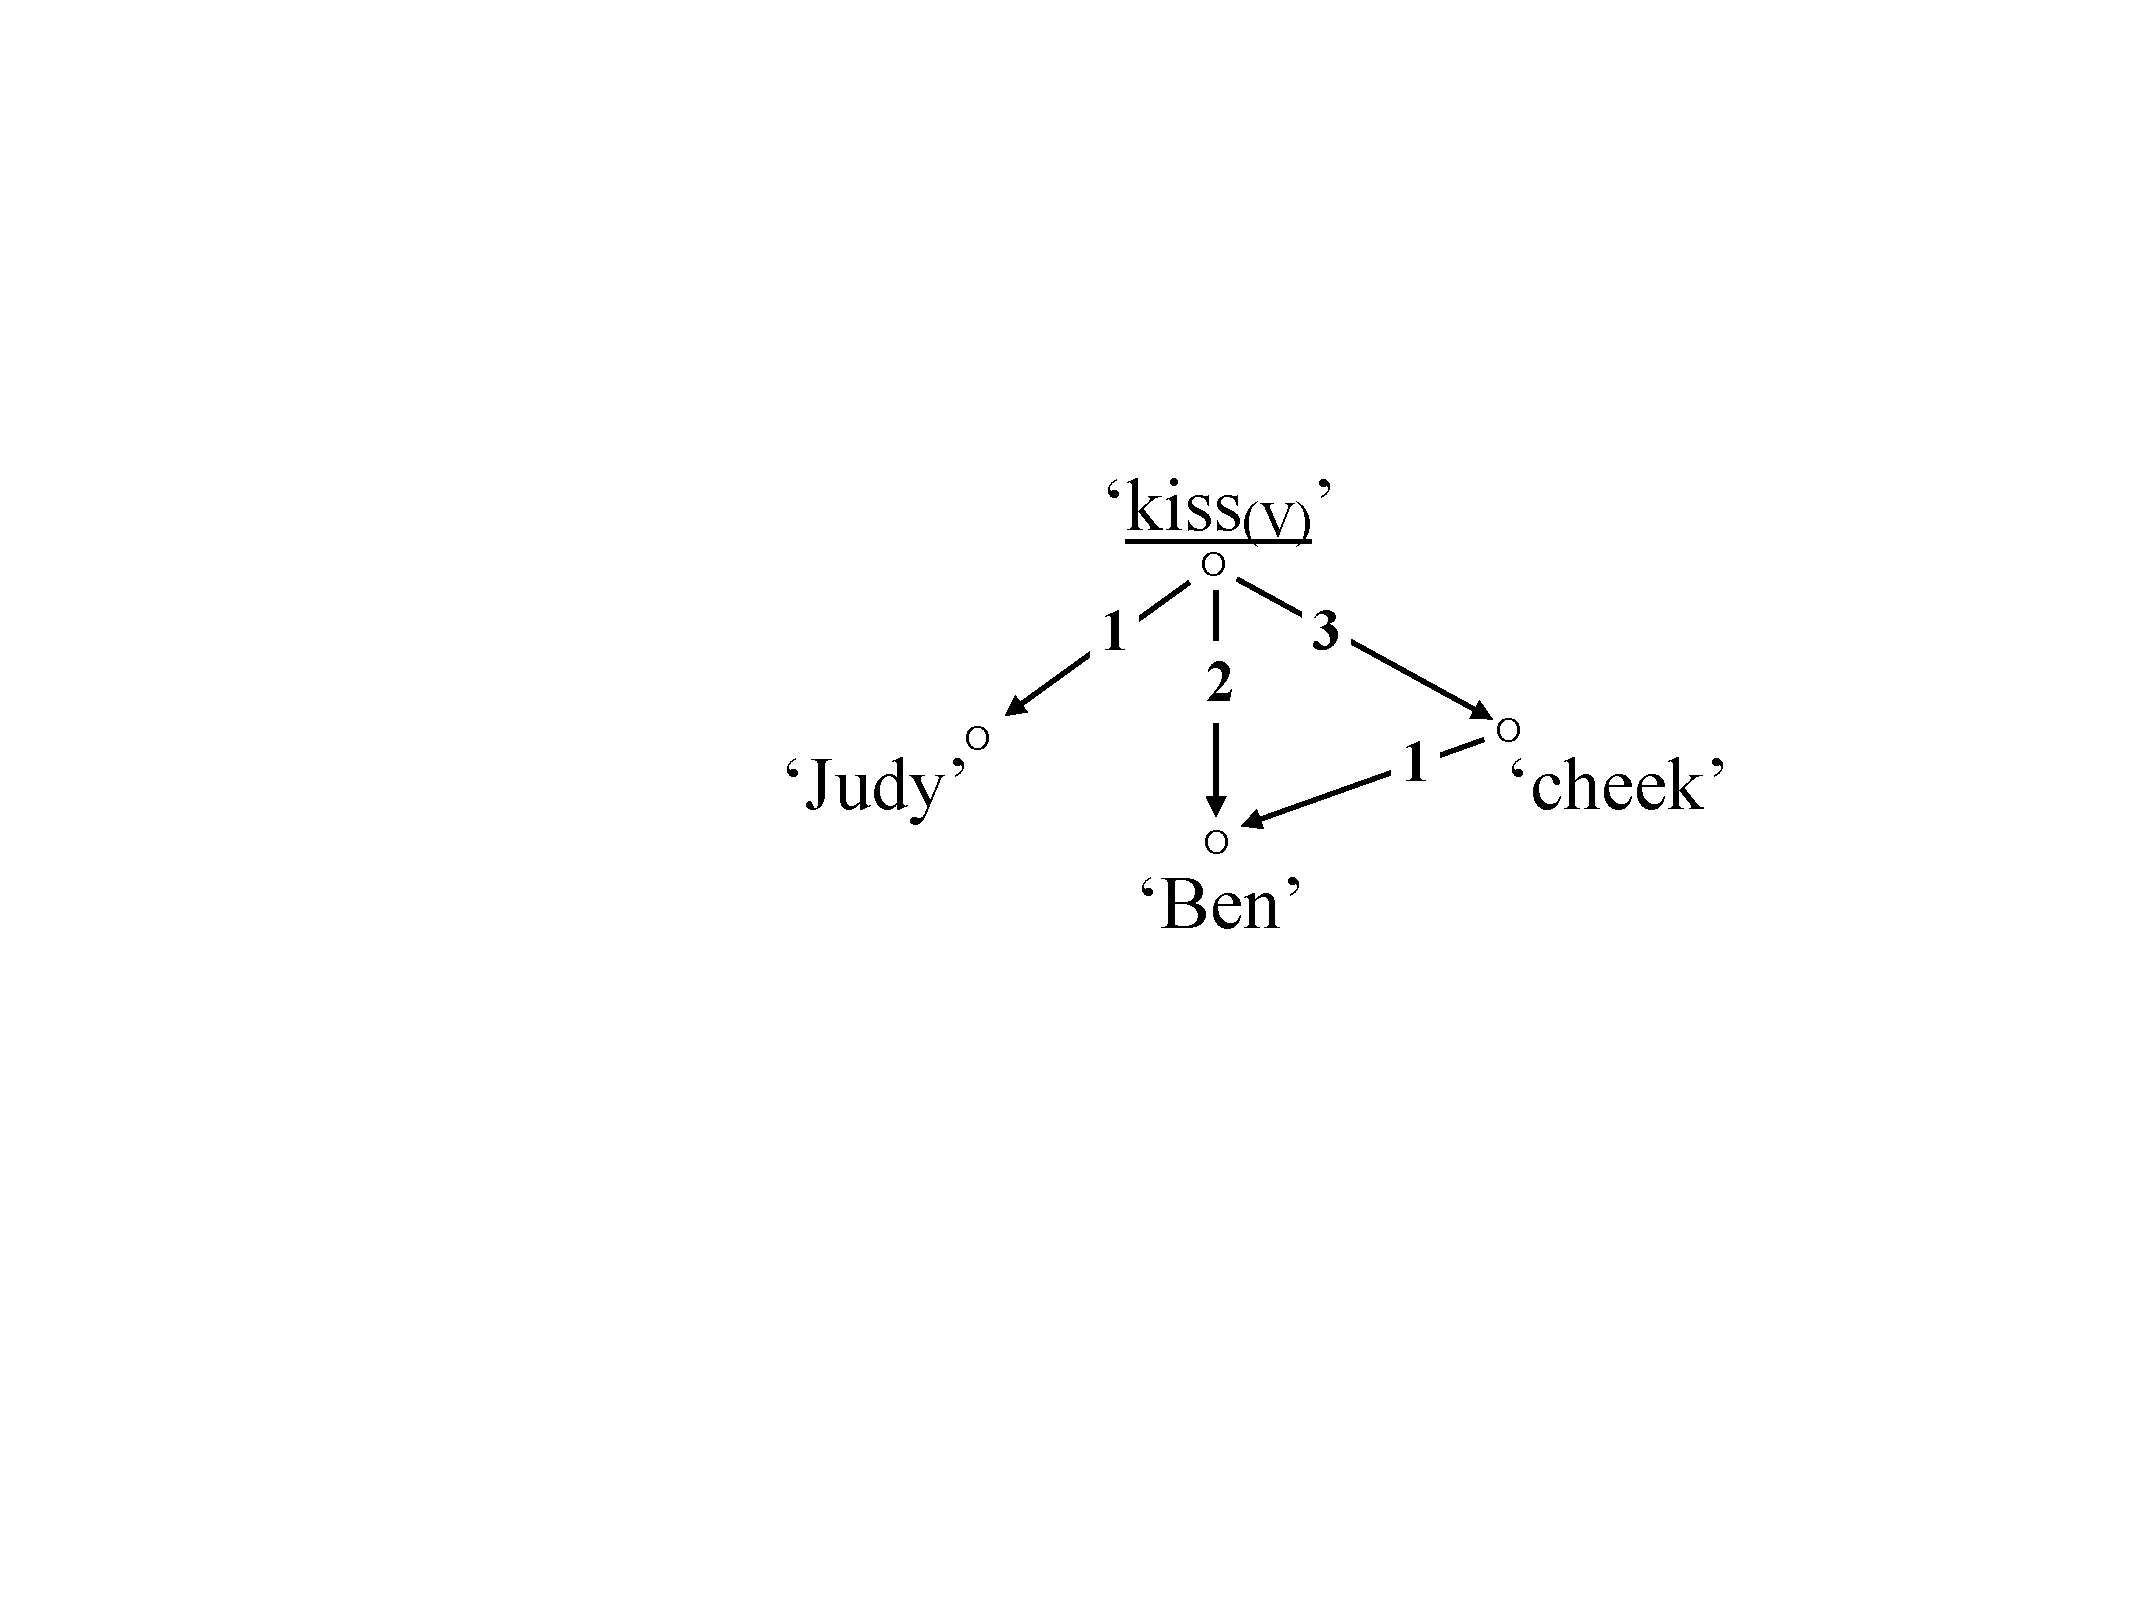
\includegraphics[width=4.5cm]{Fig/PrelimNotions/SemSJudyKissedBenCheek.pdf}
\caption{Semantic structure [SemS] of the sentence \textit{Judy kissed Ben on the cheek.}}\label{fig:SemSJudyKissedBenCheek}
\end{figure}

\noindent
The configuration of semantemes seen in \figref{fig:SemSJudyKissedBenCheek} is the \notion{semantic structure}\index[notion]{structure!semantic \tld\ [SemS]|emph}\index[notion]{semantic!\tld\ structure [SemS]|emph} [\notion{SemS}] of sentence \ref{ex:JudyKissedBenOnCheek} and of all its paraphrases\index[notion]{paraphrase}.\footnote{On paraphrasing, see \chapref{chap:NotionLF}, \sectref{sec:LFStandardParaphrasing} (p.\thinspace\pageref{sec:LFStandardParaphrasing}).} It calls for the following three comments.

\begin{quote}

\remark{Note.}The SemS in \figref{fig:SemSJudyKissedBenCheek} does not encode inflectional\index[notion]{inflection} meanings, that is, \notion{grammemes}\index[notion]{grammeme|emph} expressed in \ref{ex:JudyKissedBenOnCheek}: the indicative and the past tense of the verb \textsc{kiss}\tsub{(V)}, as well as the singular of the noun \textsc{cheek}. For simplicity's sake, we follow the same policy in all SemSs in this volume.

\end{quote}

\paragraph*{1) Communicatively dominant semanteme.}

The sentence \textit{Judy kissed Ben on the cheek} is about an act of kissing: therefore, the semanteme `\myuline{kiss}' is \notion{communicatively dominant}\index[notion]{communicative!\tld\ dominance|emph}, which is indicated by underscoring. By contrast, the noun phrase \textit{Ben's cheek that was kissed by Judy} is about the cheek (of Ben) and possesses an identical semantic structure, except for the semanteme `\myuline{cheek}', which is communicatively dominant (i.e., underscored in the semantic structure of this phrase).

Communicative dominance is an essential component of the \notion{communicative structure}\index[notion]{communicative!\tld\ structure|emph}\index[notion]{structure!communicative \tld|emph} of utterances, as theorized in \textcite{Polguere1990a-e} and \textcite{Melcuk2001b}. For the sake of simplicity, other components of communicative structures -- such as the Rheme\index[notion]{Rheme} vs. Theme\index[notion]{Theme} opposition -- are not encoded in utterance representations in this volume.

\paragraph*{2) Semantic actants' numbering.}

Numbering of SemAs of a predicative meaning depends on its internal structure, that is, on its semantic decomposition. Kissing someone is to act upon someone, and the Agent\index[notion]{Agent (semantic role)}\index[notion]{semantic!\tld\ role} of an action is taken to be SemA~\syntDname{1}, the Patient\index[notion]{Patient (semantic role)} undergoing an action is SemA~\syntDname{2}, and the Target\index[notion]{Target (semantic role)} of the kiss (part of the Patient's body) is SemA~\syntDname{3}.

\paragraph*{3) Semantic structure as a network.}

\figref{fig:SemSJudyKissedBenCheek} shows that the SemA~\syntDname{3} of `kiss' is a quasi-predicate that controls one actant slot: `cheek of X'. This is due to the fact that `cheek' is `part of the body of X [such that...]'; all names of body parts necessarily express quasi-predicative semantemes.  In this case, the SemA~\syntDname{1} of the quasi-predicate `cheek' is `Ben', and `Ben' is itself the SemA~\syntDname{2} of `kiss'. This configuration of semantic dependencies forms a \notion{semantic network}\index[notion]{semantic!\tld\ network|emph}\index[notion]{network \lfgp{see also \textit{graph}}!semantic \tld|emph}.

\begin{furtherreading}
On semantemes\index[notion]{semanteme}, see \textcite{MelcukPolguere2008}, \textcite{Polguere2012a} and \textcite[Part~II, Sec.~2.2, 193--205]{Melcuk2012a-e}; on communicative dominance\index[notion]{communicative!\tld\ dominance}, see \textcite[Part~I, Sec.~2.3.1.1]{Melcuk2001b}; on SemA numbering\index[notion]{actant!semantic \tld\ number}, see \textcite[Ch.~12, Sec.~3.4.2.3]{Melcuk2015a-e} and \textcite[Ch.~4, Sec.~3]{Melcuk2012a-e}; on Meaning-Text semantic networks, see \textcite{Polguere1997-e}.
\end{furtherreading}

\section{Syntactic notions}\label{sec:syntacticNotions}

From the viewpoint of syntactic structures, two levels of representation are distinguished, which can be approximately characterized as follows.

The \notion{deep-syntactic structure}\index[notion]{structure!deep-syntactic \tld\ [DSyntS]|emph}\index[notion]{deep-syntactic!\tld\ structure [DSyntS]|emph}\index[notion]{syntax!deep \tld|emph} [\notion{DSyntS}]\phantomsection\label{txt:DSyntS} is the most direct lexical and syntactic expression of the corresponding SemS. It contains only the semantically full lexical units of the sentence to be produced, connected by labeled \notion{deep-syntactic dependencies}\index[notion]{dependency!deep-syntactic \tld}, called \notion{deep-syntactic relations}\index[notion]{deep-syntactic!\tld\ relation}\index[notion]{relation!deep-syntactic \tld}. The resulting structure is a \notion{dependency tree}\index[notion]{dependency!\tld\ tree}\index[notion]{tree!dependency \tld}\index[notion]{tree!deep-syntactic \tld}\index[notion]{deep-syntactic!\tld\ tree}.

The \notion{surface-syntactic structure}\index[notion]{structure!surface-syntactic \tld\ [SSyntS]|emph}\index[notion]{surface-syntactic!\tld\ structure [SSyntS]|emph}\index[notion]{syntax!surface \tld|emph} [\notion{SSyntS}] is geared to the actual sentence in the sense that it serves to determine word order\index[notion]{word order} and morphological dependencies\index[notion]{dependency!morphological \tld}\index[notion]{morphology!morphological dependency} between lexemes, if any. It contains all and only the lexemes of the sentence to be produced, connected by labeled surface-syntactic dependencies, called \notion{surface-syntactic relations}\index[notion]{surface-syntactic!\tld\ relation}\index[notion]{relation!surface-syntactic \tld}. The resulting structure is, of course, also a dependency tree.

Let us illustrate the \notion{correspondences}\index[notion]{correspondence between representation levels|emph} between the SemS, the DSyntS and the SSyntS of a sentence, using sentence \Next as example.

\begingroup
\small

\ex. Judy shoots the breeze with Ben for hours.\label{ex:JudyShootsBreezeBenForHours}

\endgroup

``A\thinspace$\Leftrightarrow$\thinspace{}B'' means `linguistic entity A of the level $n$ of representation corresponds, i.e. is semantically equivalent, to linguistic entity B of level $n+1$; for instance, \figref{fig:sampleSemDSyntCorr} shows the SemS\thinspace$\Leftrightarrow$\thinspace{}DSyntS correspondence for \textit{Joey sleeps}.

\noindent
\begin{figure}

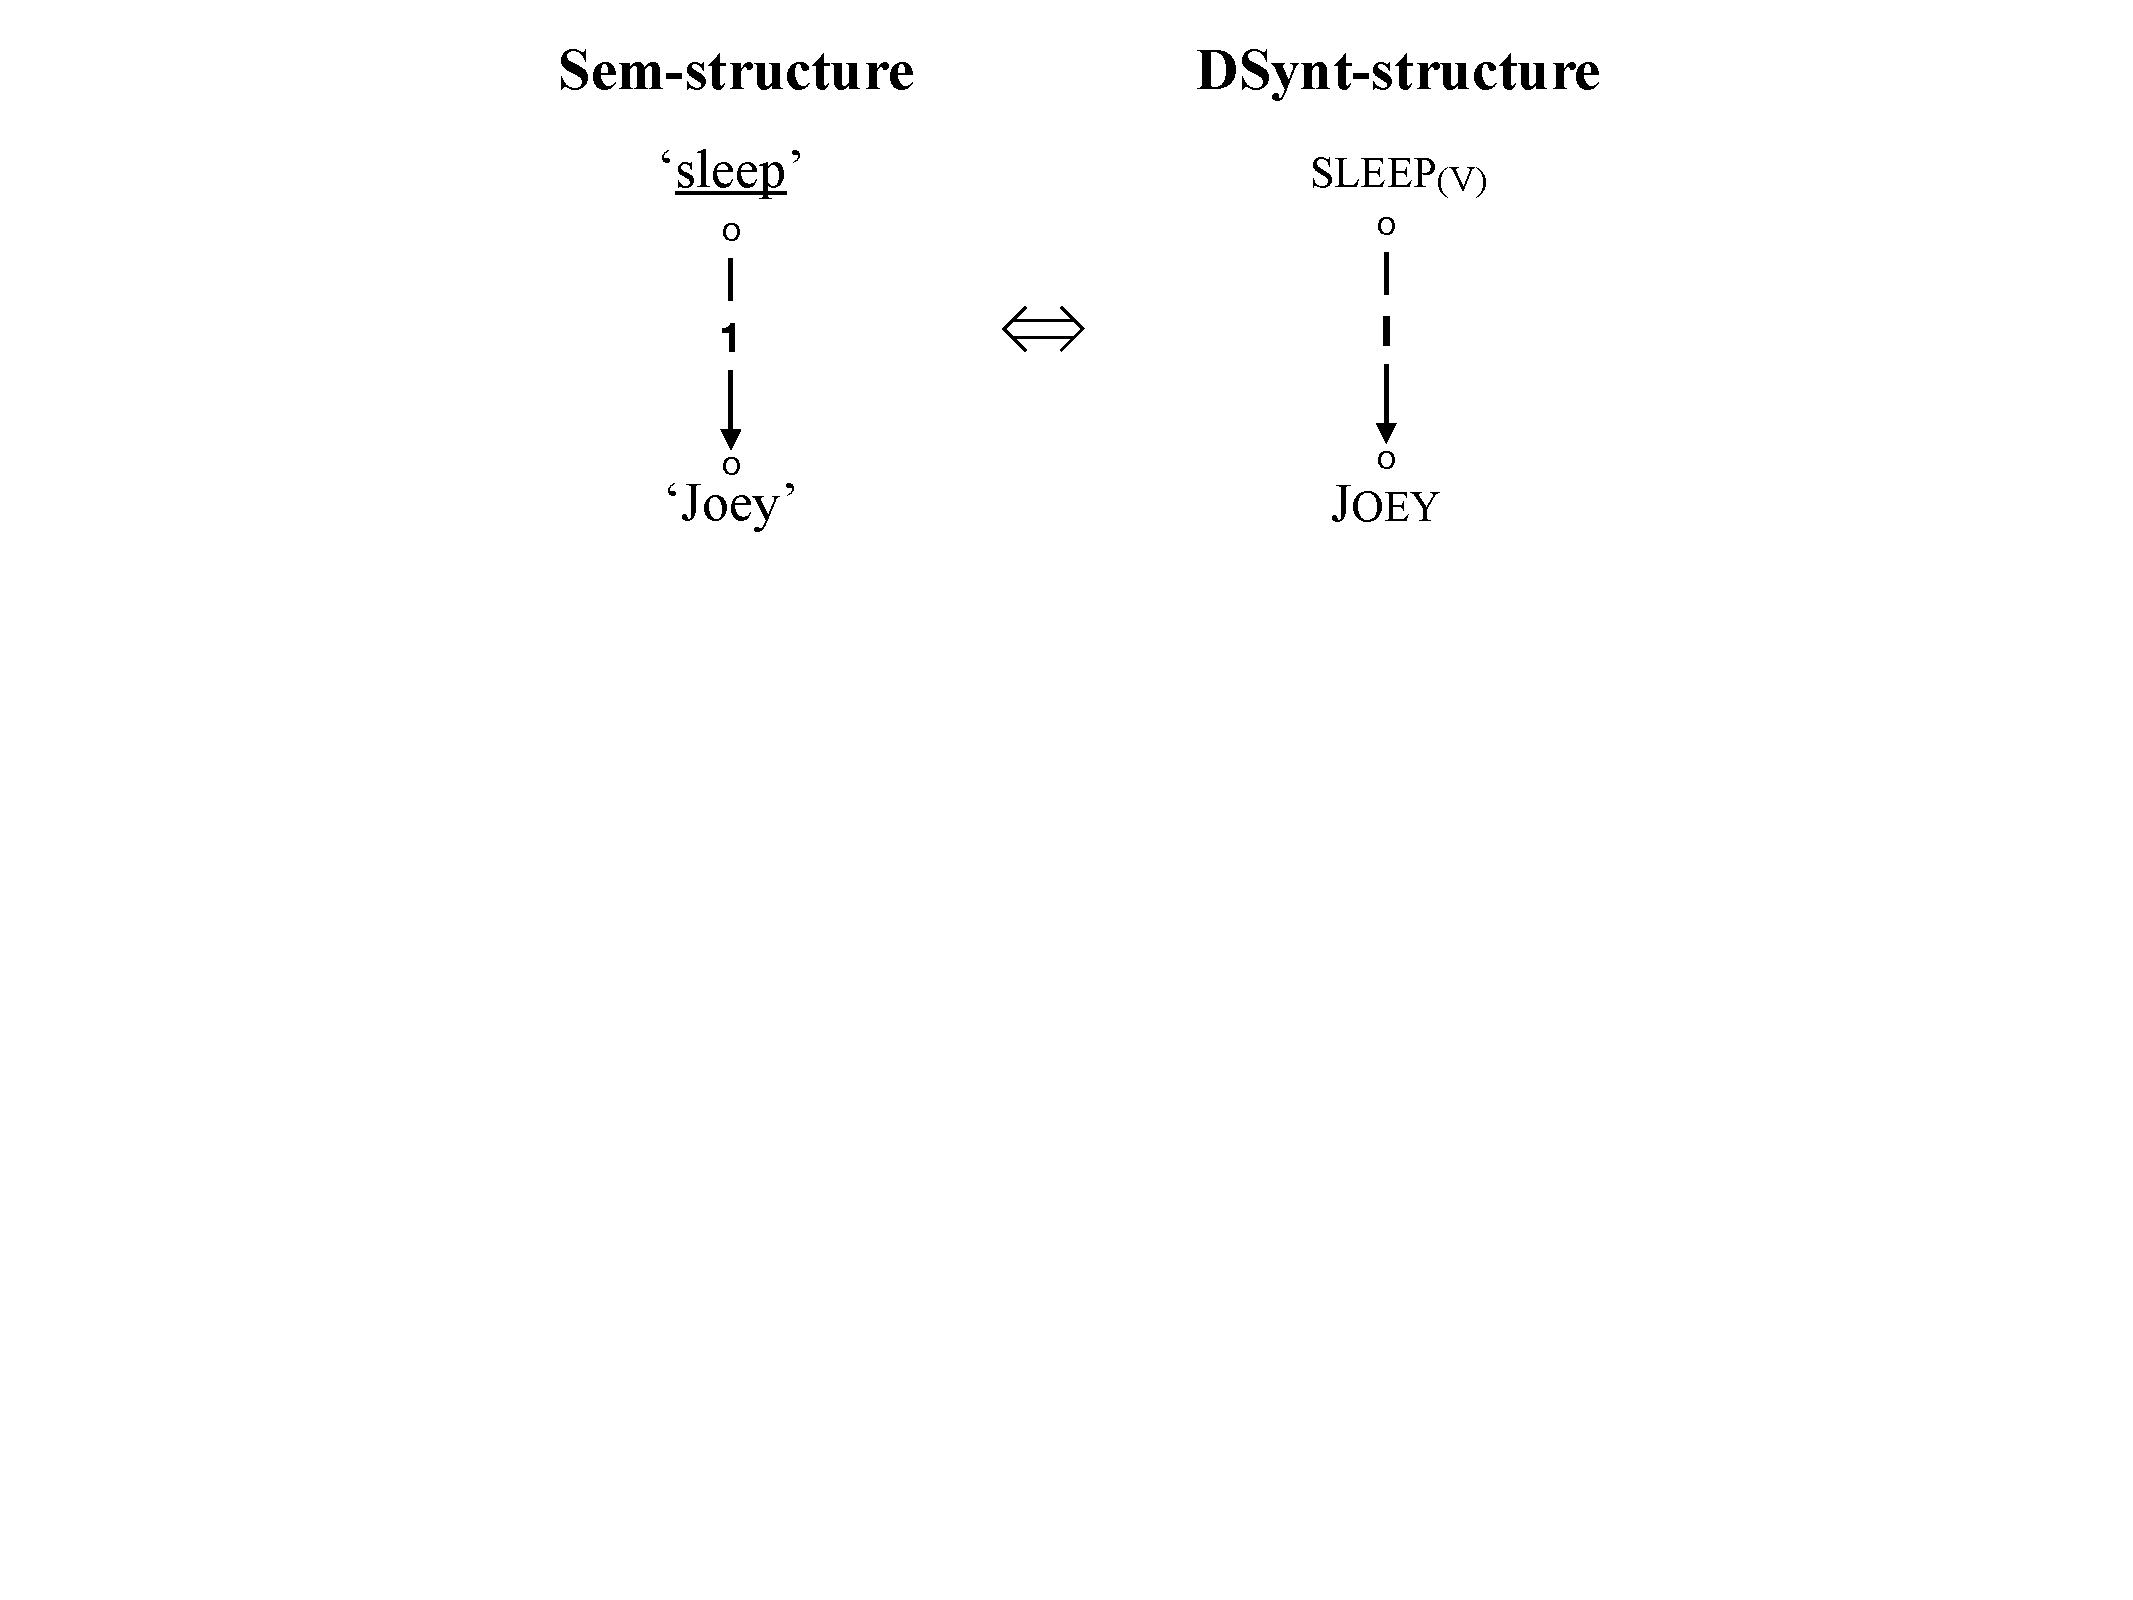
\includegraphics[width=6.5cm]{Fig/PrelimNotions/sampleSemDSyntCorr.pdf}
\caption{Example of a SemS\thinspace$\Leftrightarrow$\thinspace{}DSyntS correspondence}\label{fig:sampleSemDSyntCorr}
\end{figure}

In what follows we focus on  two particular correspondences between utterance structures: SemS\thinspace$\Leftrightarrow$\thinspace{}DSyntS and DSyntS\thinspace$\Leftrightarrow$\thinspace{}SSyntS.

\noindent
\begin{figure}

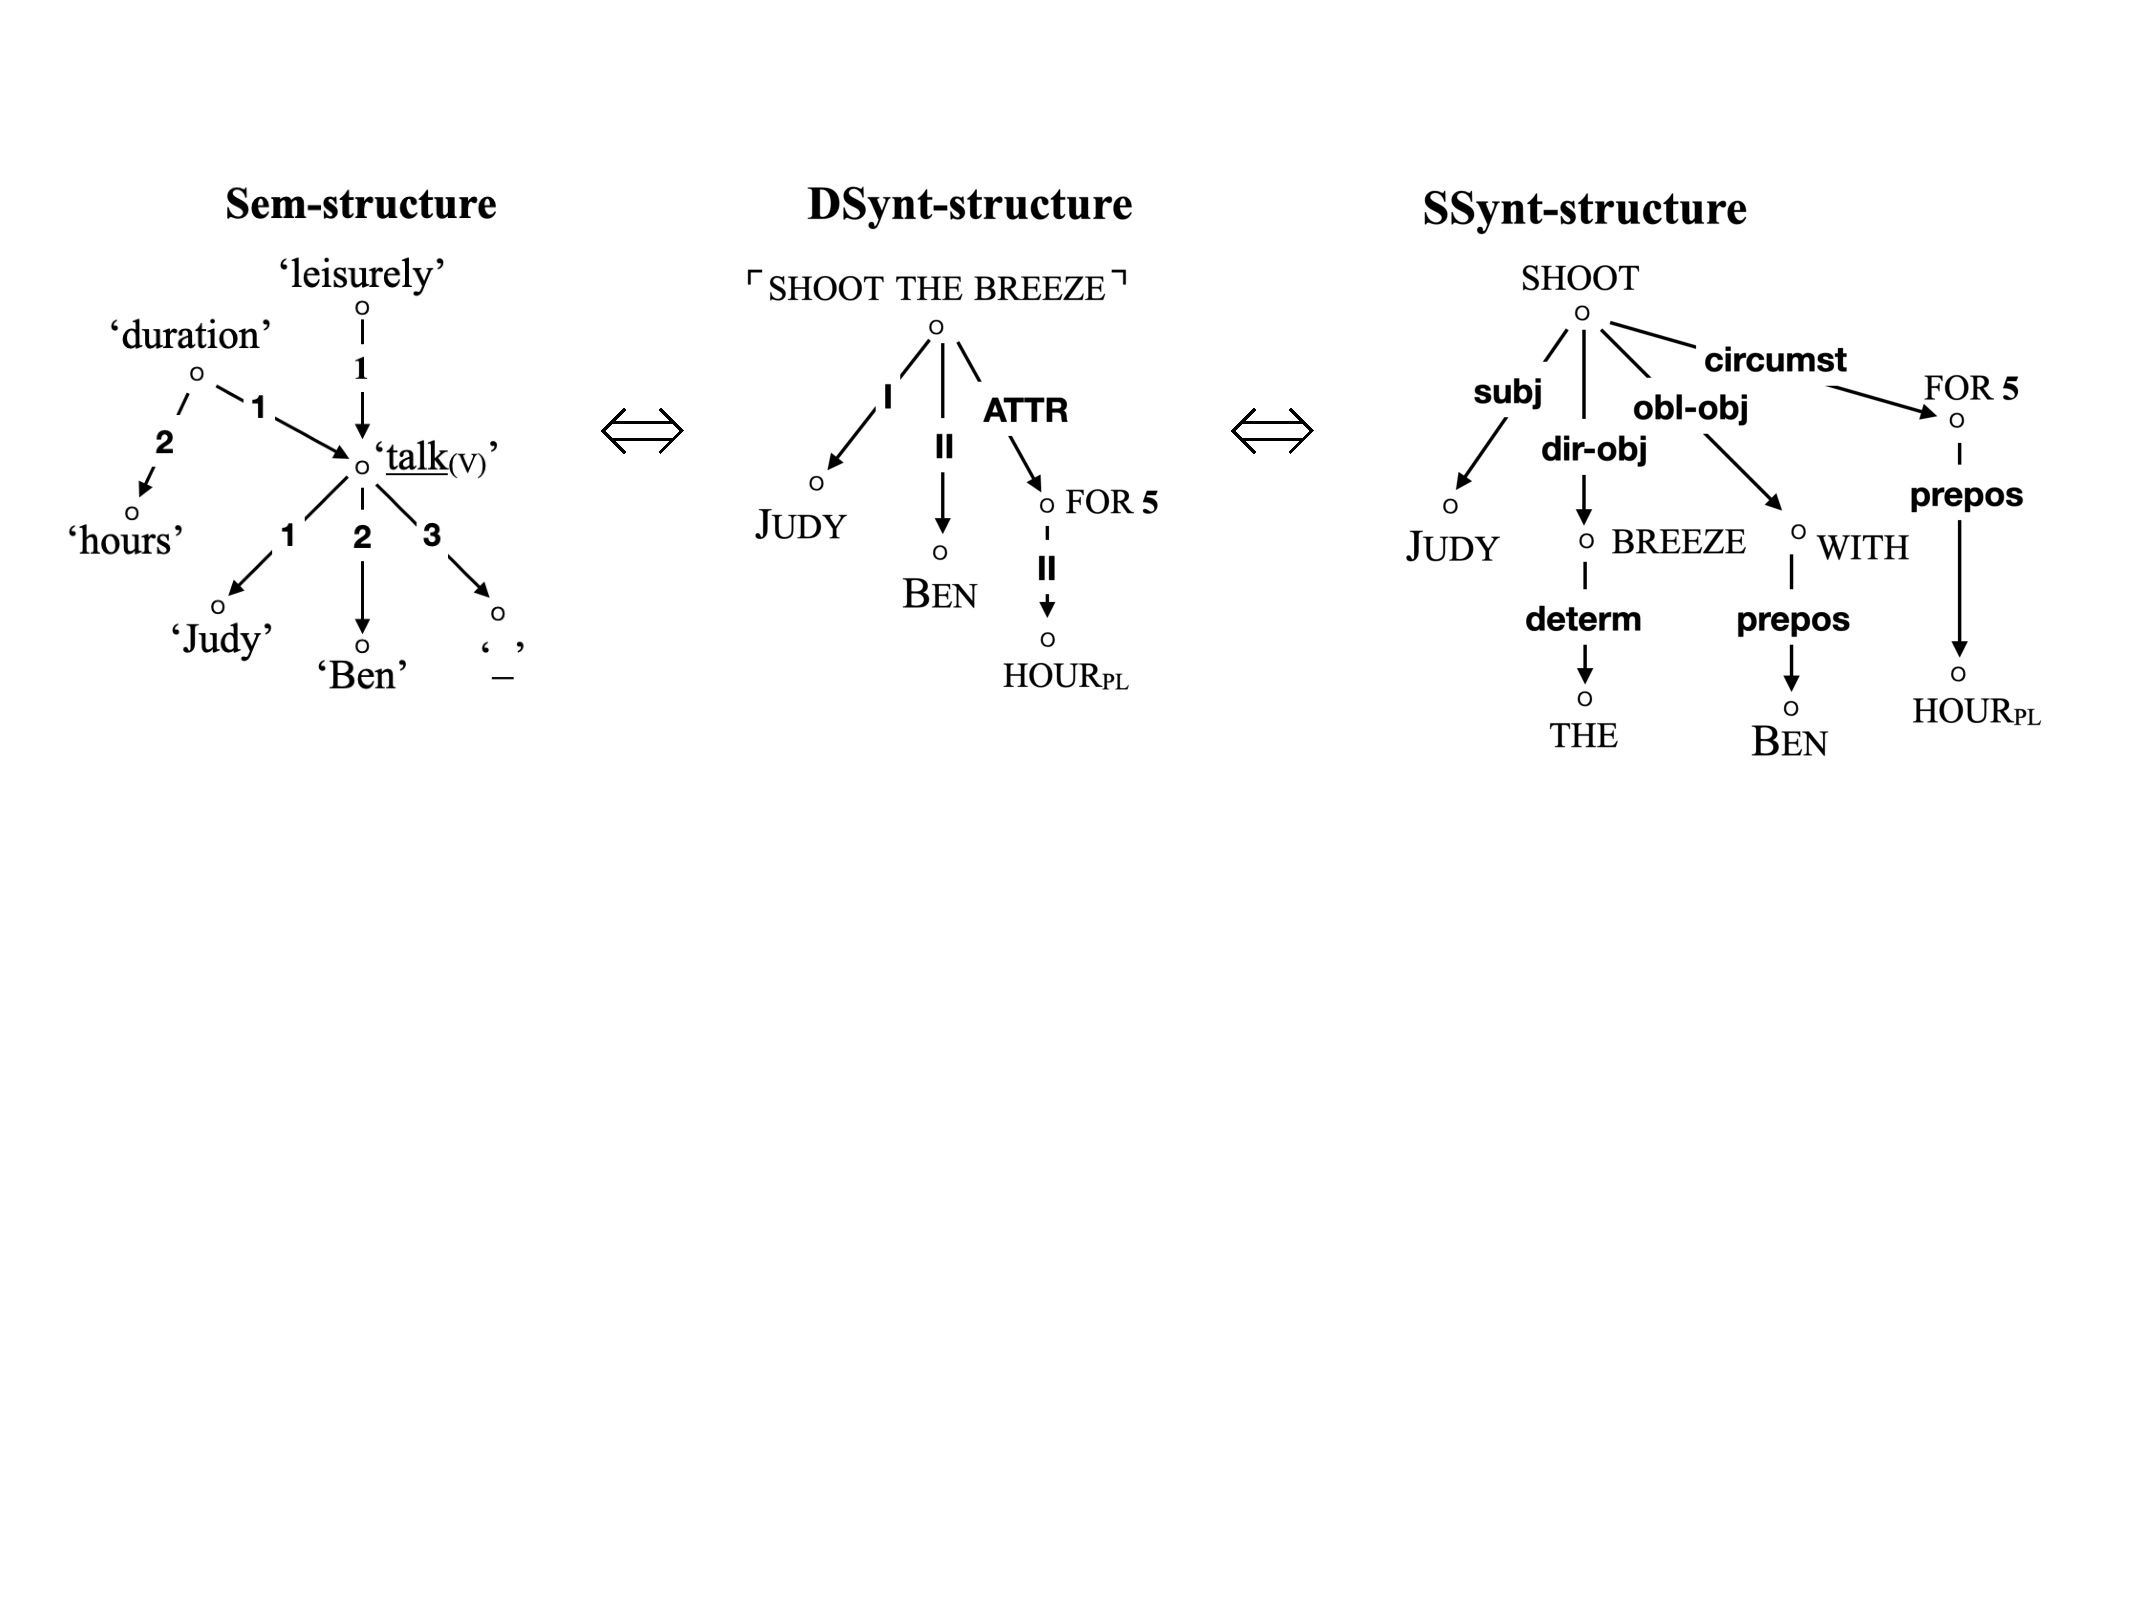
\includegraphics[width=\linewidth]{Fig/PrelimNotions/SemDSyntSSyntCorr.pdf}
\caption[SemS\thinspace$\Leftrightarrow$\thinspace{}DSyntS\thinspace$\Leftrightarrow$\thinspace{}SSyntS correspondences for the sentence\newline \textit{Judy shoots the breeze with Ben for hours.}]{SemS\thinspace$\Leftrightarrow$\thinspace{}DSyntS\thinspace$\Leftrightarrow$\thinspace{}SSyntS correspondences for sentence \ref{ex:JudyShootsBreezeBenForHours}: \textit{Judy shoots the breeze with Ben for hours.}}\label{fig:SemDSyntSSyntCorr}
\end{figure}

The SemS\index[notion]{semantic!\tld\ structure [SemS]}\index[notion]{structure!semantic \tld\ [SemS]} has been introduced and explained in \sectref{sec:semanticNotions}. Here we need to explain the DSyntS and the SSyntS.

\paragraph*{Deep-syntactic structure [DSyntS] of sentence \ref{ex:JudyShootsBreezeBenForHours}.}\index[notion]{deep-syntactic!\tld\ structure [DSyntS]}\index[notion]{structure!deep-syntactic \tld\ [DSyntS]}

The nodes of this tree\index[notion]{tree!deep-syntactic \tld|emph}\index[notion]{deep-syntactic!\tld\ tree|emph} are labeled with \notion{deep lexical units}\index[notion]{lexical unit!deep \tld|emph}, i.e., semantically full lexical units, which express semantemes of the SemS. The idiom \idiom{\textsc{shoot the breeze}} expresses the semantic configuration `leisurely\thinspace\syntRel{1}\thinspace\myuline{talk}\tsub{(V)}', and the meaningful preposition\index[notion]{preposition} \textsc{for}\sensenum{5}, the semanteme `duration'.\footnote{The lexicographic number of \textsc{for}\sensenum{5} comes from the online \textit{Longman Dictionary of Contemporary English} \parencite{Longman2025}, henceforth LDOCE.}\index[notion]{dictionary!Longman Dictionary of Contemporary English@\textit{Longman Dictionary of Contemporary English} [LDOCE]}\index[notion]{Longman Dictionary of Contemporary English@\textit{Longman Dictionary of Contemporary English} [LDOCE]}\index[notion]{lexicographic number} The other nodes are self-explanatory.

The arcs (branches) of this tree are labeled with DSynt-relations of two types:

\begin{itemize}

\item \syntDname{I} and \syntDname{II} are \notion{actantial DSynt-relations}\index[notion]{actantial relation|emph}\index[notion]{relation!actantial \tld|emph}: the dependent\index[notion]{dependent, syntactic} members of these relations -- \textsc{Judy} and \textsc{Ben} -- are DSynt-actants\index[notion]{actant!deep-syntactic \tld\ [DSyntA]}\index[notion]{deep-syntactic!\tld\ actant [DSyntA]} of their governor, the idiom \idiom{\textsc{shoot the breeze}} (`X \idiom{shoots the breeze} with Y'). The notion of DSynt-actant will be defined shortly (p.\thinspace\pageref{def:DSyntA}).

\item \syntDname{ATTR}\index[notion]{ATTR@\syntDname{ATTR}|emph}\phantomsection\label{txt:ATTRDSyntR} is a non-actantial DSynt-relation: it is not foreseen by the meaning of its governor\index[notion]{governor, syntactic} and represents a dependency inversion -- called \notion{head-switching}\index[notion]{head-switching} -- with respect to the corresponding semantic relation; cf.~\figref{fig:SDSyntSDependencyInversion}.

\end{itemize}

\begin{figure}

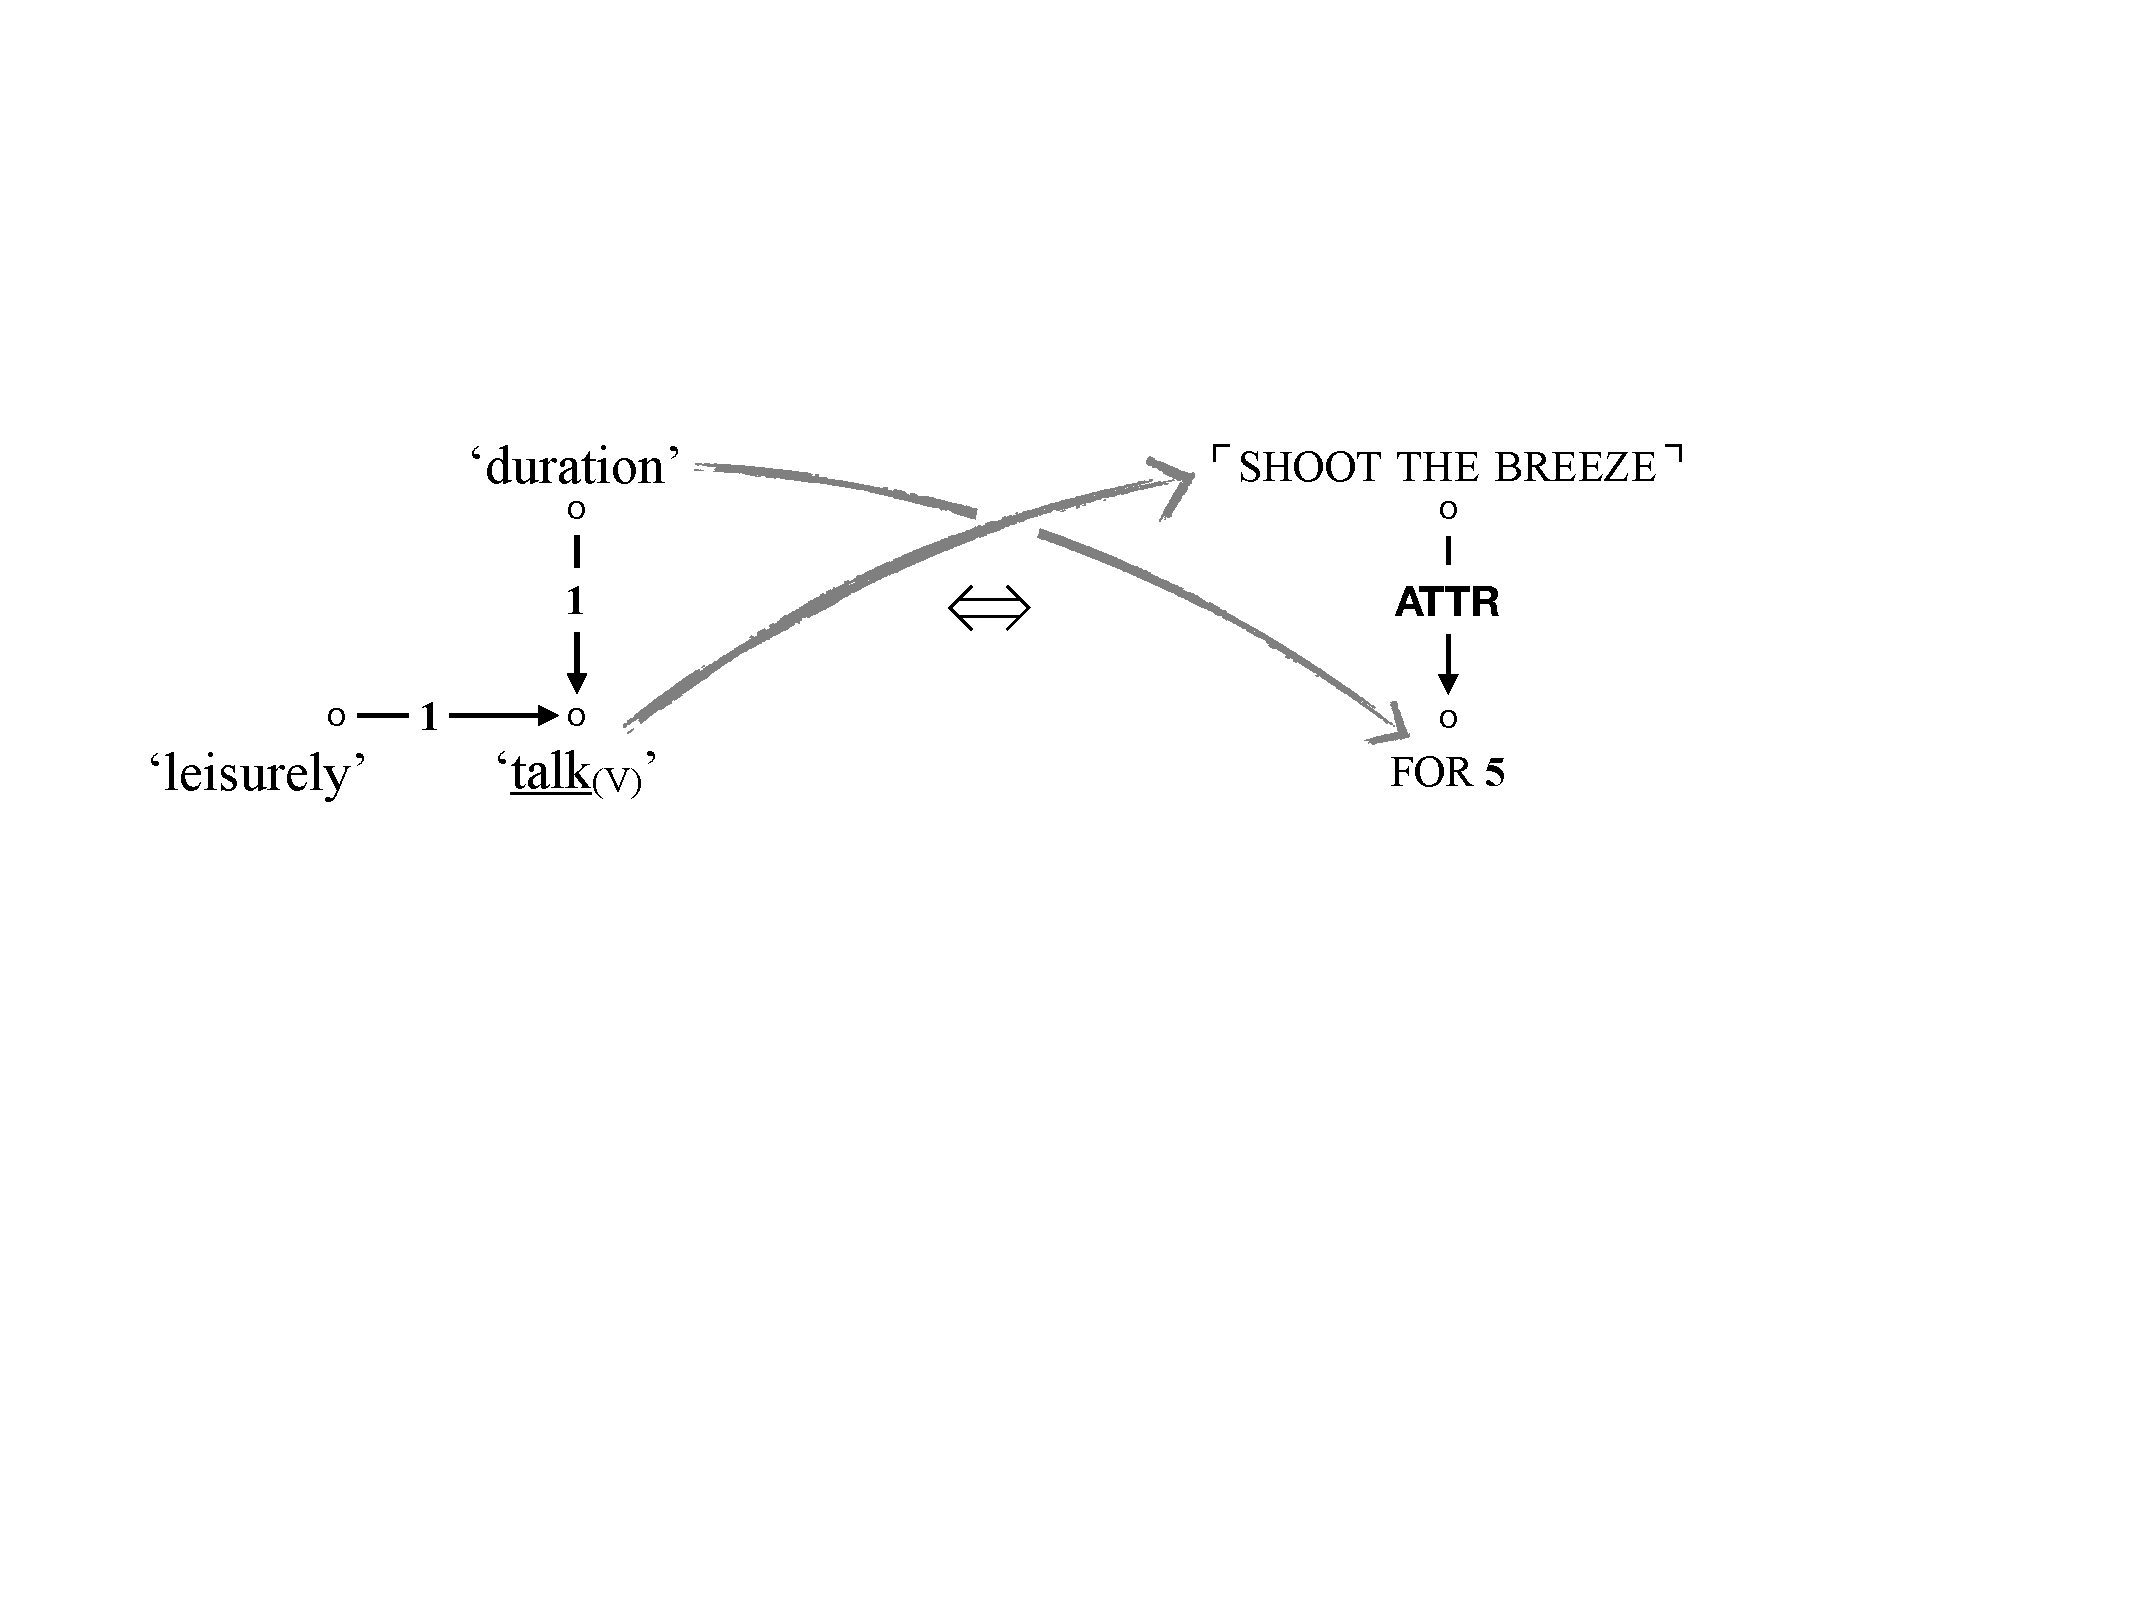
\includegraphics[width=10.5cm]{Fig/PrelimNotions/SemSDSyntSDependencyInversion.pdf}
\caption[SemS\thinspace$\Leftrightarrow$\thinspace{}DSyntS dependency inversion \[=~head-switching\]\newline involving the DSynt-relation \syntDname{ATTR}]{SemS\thinspace$\Leftrightarrow$\thinspace{}DSyntS dependency inversion [=~head-switching] involving the \mbox{DSynt-relation} \syntDname{ATTR}}\label{fig:SDSyntSDependencyInversion}
\end{figure}

At the DSynt-level several other DSynt-relations are used -- they are listed below. These relations are language-universal\index[notion]{language-universal}. In the present volume only actantial and \syntDname{ATTR}(ibutive) DSynt-relations are relevant.

\phantomsection\label{tab:listDSyntRels}\begin{soundbox}{Language-universal DSynt-relations}
\vspace{-14pt}
\small
\setlength{\tabcolsep}{3pt}
\setlength\extrarowheight{1pt}
\begin{longtable}{ l >{\raggedright\arraybackslash}p{8.8cm} }

\syntDname{I} & 1\tsup{st} deep-syntactic relation\slashs1\tsup{st} deep-syntactic actant \\*
\syntDname{II} & 2\tsup{nd} deep-syntactic relation\slashs2\tsup{nd} deep-syntactic actant [\textit{Joey}\thinspace\syntRelLeft{I}\thinspace\textit{loves}\thinspace\syntRel{II}\thinspace\textit{food}] \\*
\syntDname{...} & \\[+3pt]

\syntDname{APPEND} & appenditive; it links an structurally extraneous element, such as a parenthetical or an interjection\index[notion]{interjection}, to its governor\index[notion]{governor, syntactic} -- the syntactic head of the clause [\textit{Sorry,}\thinspace\syntRelLeft{APPEND}\syntRelChunk{{\relsize{-1.5}[\textit{I}]}}\thinspace\textit{am late}] \\

\syntDname{ADDRESS} & addressative; it links a direct address to its governor, which is the syntactic head of the clause [\textit{Yes,}\thinspace\syntRel{ADDRESS}\thinspace\textit{Sir}] \\

\syntDname{ATTR} & attributive; it links a restrictive modifier\slashs{}circumstantial to its governor [\textit{curious}\thinspace\syntRelLeft{ATTR}\thinspace\textit{student}; \textit{arrived}\thinspace\syntRel{ATTR}\thinspace\textit{yesterday}] \\

\syntDname{ATTR\tsub{qual}} & qualificative attributive; it links a qualificative modifier\thinspace/ circumstantial to its governor [\textit{students,}\thinspace \syntRel{ATTR\tsub{qual}}\thinspace\textit{hungry for knowledge}] \\

\syntDname{COORD} & coordinative; it links the dependent\index[notion]{dependent, syntactic} member of a syntactic coordination to its governor [\textit{Ben}\thinspace\syntRel{COORD}\thinspace\textit{and Judy}] \\

\syntDname{PSEUDO-COORD} & pseudo-coordinative; it links the dependent member of elaboration or clarification to its governor \\*
& [\textit{She came last year,}\thinspace\syntRel{PSEUDO-COORD}\thinspace\textit{in the spring}] \\

\end{longtable}
\end{soundbox}\index[notion]{circumstantial}

A notion playing a key role in the presentation of lexical functions is that of \notion{deep-syntactic actant}\index[notion]{actant!deep-syntactic \tld\ [DSyntA]|emph}\index[notion]{deep-syntactic!\tld\ actant [DSyntA]|emph} [\notion{DSyntA}]\index[notion]{DSyntA [deep-syntactic actant]|see{actant (deep-syntactic)}}, mentioned above. It is defined as follows.

\begin{notiondefinition}{deep-syntactic actant [DSyntA]}
\phantomsection\label{def:DSyntA}A \notion{deep-syntactic actant} \syntDname{I}, \syntDname{II}, ... of lexical unit L is a DSynt-dependent\index[notion]{dependent, syntactic} of L such that\vspace{3pt} \\*
\setlength{\tabcolsep}{.5pt}\begin{tabular}{ p{0.2cm} >{\raggedright\arraybackslash}p{11cm} }
\SpecDiff & it expresses, in a prototypical case, a SemA of L and it is governed by L via an actantial DSynt-relation \syntDname{I}, \syntDname{II}, ... \\
\end{tabular}
\end{notiondefinition}

There is also a frequent enough possibility of a DSyntA of L coming, or being raised, to L from one of its DSyntAs. Such \notion{syntactic raising}\index[notion]{raising, syntactic} is illustrated in \figref{fig:DSyntARaising}. This figure presents one of the support verbs\index[notion]{support verb}\index[notion]{verb!support \tld} mentioned in \chapref{chap:Introduction} (\sectref{sec:aboutWhat}), namely the lexical function \lf{Oper\tsub{1}}\index[lf]{Operi@\lf{Oper\tsub{i}}!\lf{Oper\tsub{1}}} (\chapref{chap:syntLFs}, [\ref{lf:Oper-i}], p.\thinspace\pageref{lf:Oper-i}).

\lfappl{Oper\tsub{1}}{\textit{attack}\tsub{(N)}} is expressed in the surface-syntactic structure\index[notion]{surface-syntactic!\tld\ structure [SSyntS]}\index[notion]{structure!surface-syntactic \tld\ [SSyntS]} (see SSyntS below) by the lexical units \idiom{\textsc{carry out}} or \textsc{conduct}\tsub{(V)}. The \notion{actant transfer}\index[notion]{actant!transfer of deep-syntactic \tld} illustrated in \figref{fig:DSyntARaising} is common with verbal syntagmatic lexical functions (support and realization verbs) -- see \chapref{chap:syntLFs}, ``\nameref*{par:transferOfLsActants},'' p.\thinspace\pageref{par:transferOfLsActants}.

\begin{quote}
\remark{Remark.}\phantomsection\label{remark:raising}The second sentence (with raising) in \figref{fig:DSyntARaising} is dubious: speakers seem to accept it only with a special prosody, namely, pauses before and after \textit{on the fort}: \textit{The enemy carried out -- on the fort -- a massive attack}. Other languages, such as French and Russian, allow for this construction without problem, as shown in \Next[a-b].
\end{quote}

\begingroup
\small

\ex. \a. {\smaller French} L'ennemi a mené contre le fort une attaque massive.
     \b. {\smaller Russian} Vrag provël na fort massirovannuju ataku.

\endgroup

\begin{figure}
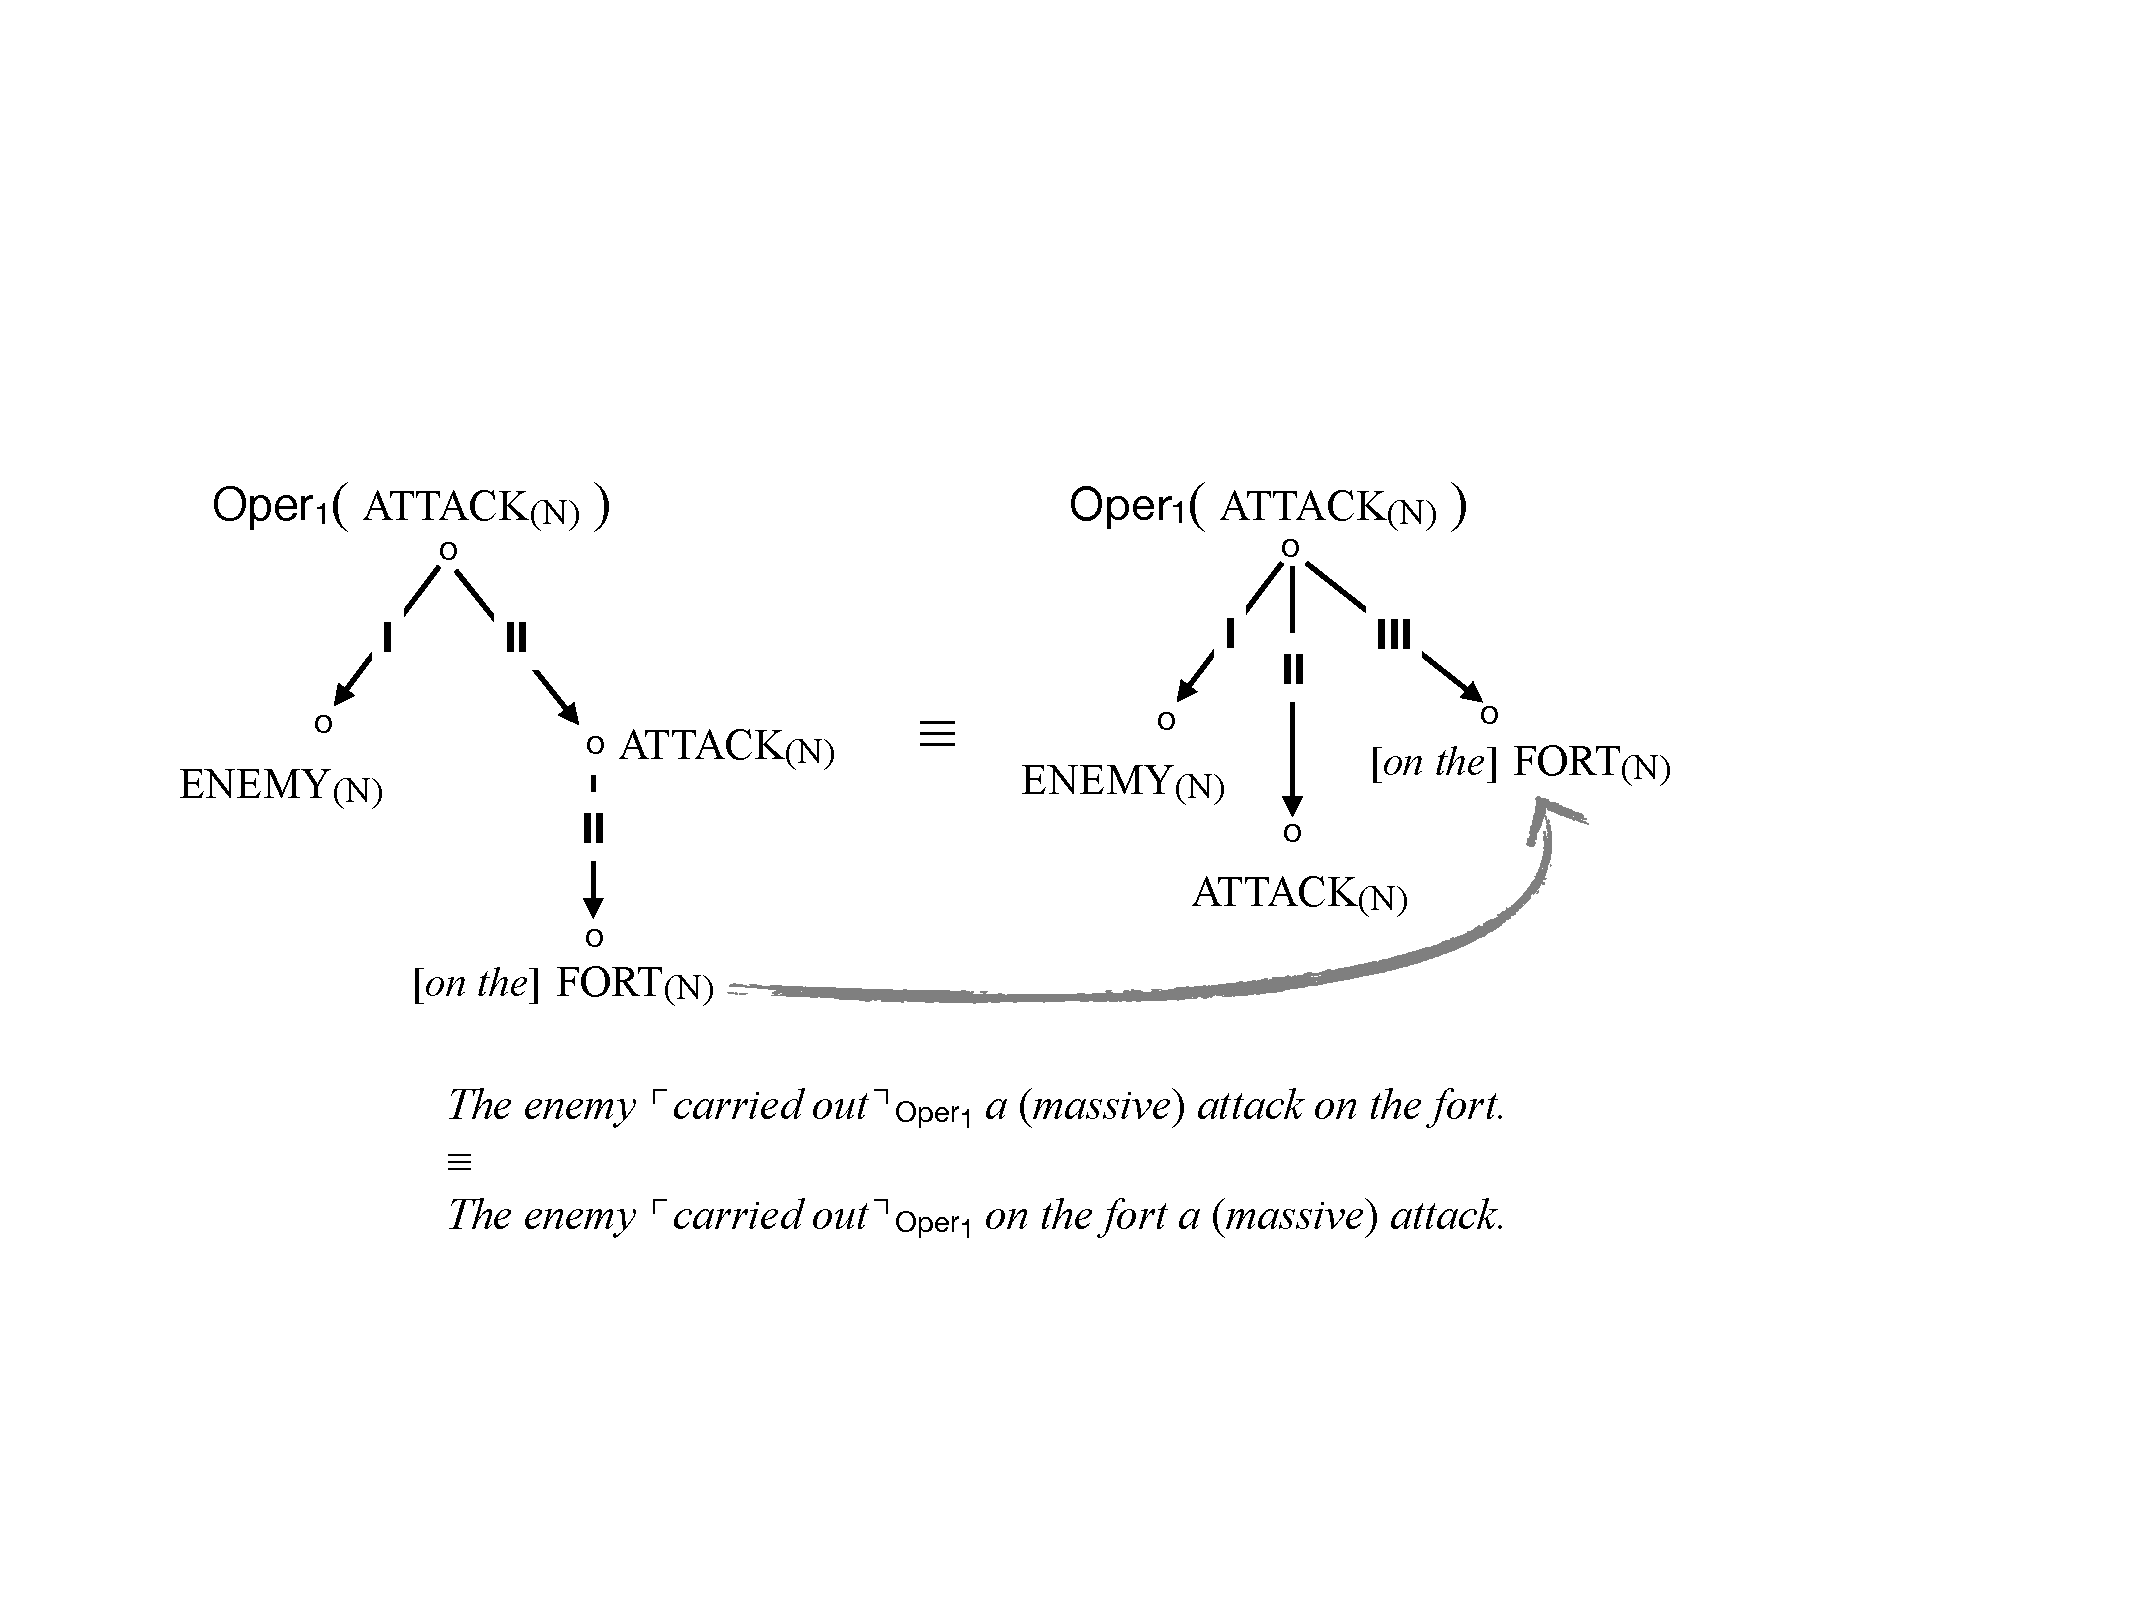
\includegraphics[width=11cm]{Fig/PrelimNotions/DSyntARaising.pdf}
\caption{Syntactic raising of a DSyntA}\label{fig:DSyntARaising}
\end{figure}

\paragraph*{Surface-syntactic structure [SSyntS] of sentence \ref{ex:JudyShootsBreezeBenForHours}.}\index[notion]{surface-syntactic!\tld\ structure [SSyntS]}\index[notion]{structure!surface-syntactic \tld\ [SSyntS]}

The nodes of the SSynt-tree\index[notion]{tree!surface-syntactic \tld|emph}\index[notion]{surface-syntactic!\tld\ tree} for \ref{ex:JudyShootsBreezeBenForHours} are labeled with all lexemes of the sentence, including lexical components of the idiom (\textsc{shoot}, \textsc{breeze} and \textsc{the}) and a governed preposition\index[notion]{preposition} (\textsc{with}).

The arcs of this tree are labeled with SSynt-relations\index[notion]{surface-syntactic!\tld\ relation}, which are language-specific -- i.e., non-universal\index[notion]{language-universal}; there are several dozens of SSynt-relations in a language. We list below SSynt-relations featured in \figref{fig:SemDSyntSSyntCorr} (p.\thinspace\pageref{fig:SemDSyntSSyntCorr}) and in the whole volume.

\phantomsection\label{tab:listSSyntRels}\begin{soundbox}{Some SSynt-relations of English}
\vspace{-14pt}
\small
\setlength{\tabcolsep}{2.2pt}
\setlength\extrarowheight{1pt}
\begin{longtable}{ l >{\raggedright\arraybackslash}p{8.3cm} }

\syntDname{circumstantial} &  \textit{talked}\thinspace\syntRel{circumst}\thinspace\textit{for} {\relsize{-1.5}[\textit{hours}]} \\
\syntDname{determinative} &  \textit{the}\thinspace\syntRelLeft{determ}\thinspace\textit{breeze}; \textit{my}\thinspace\syntRelLeft{determ}\thinspace\textit{daughter} \\
\syntDname{direct-objectival} &  \textit{shoot}\thinspace\syntRel{dir-obj}\thinspace\textit{breeze}; \textit{Marry}\thinspace\syntRel{dir-obj}\thinspace\textit{me};\newline \textit{want}\thinspace\syntRel{dir-obj}\thinspace\textit{to} {\relsize{-1.5}[\textit{go}]}; \textit{declare}\thinspace\syntRel{dir-obj}\thinspace\textit{that} {\relsize{-1.5}[\textit{it's OK}]} \\
\syntDname{modificative} &  \textit{big}\thinspace\syntRelLeft{modif}\thinspace\textit{deal} \\
\syntDname{oblique-objectival} &  \textit{shoot} {\relsize{-1.5}[\textit{breeze}]}\thinspace\syntRel{obl-obj}\thinspace\textit{with} {\relsize{-1.5}[\textit{Ben}]}; \textit{rely}\thinspace\syntRel{obl-obj}\thinspace\textit{on} {\relsize{-1.5}[\textit{you}]} \\
\syntDname{possessive} &  \textit{tomorrow's}\thinspace\syntRelLeft{possess}\thinspace\textit{event} \\
\syntDname{prepositional} &  \textit{with}\thinspace\syntRel{prepos}\thinspace\textit{Ben}; \textit{for}\thinspace\syntRel{prepos}\thinspace\textit{hours} \\
\syntDname{subjectival} &  \textit{Judy}\thinspace\syntRelLeft{subj}\thinspace\textit{shoots} {\relsize{-1.5}[\textit{the breeze}]}; \textit{it}\thinspace\syntRelLeft{subj}\thinspace\textit{is} {\relsize{-1.5}[\textit{late}]} \\
\syntDname{subjectival-adnominal} &  \textit{speech}\thinspace\syntRel{subj-adnom}\thinspace\textit{of} {\relsize{-1.5}[\textit{the President}]} \\

\end{longtable}
\end{soundbox}\index[notion]{object, syntactic!direct \tld}\index[notion]{object, syntactic!oblique \tld}\index[notion]{subject, syntactic}\index[notion]{circumstantial}

\largerpage[-1]
\paragraph*{Active syntactic valence.}\label{para:activeSyntacticValence}

SemS\thinspace$\Leftrightarrow$\thinspace{}DSyntS\thinspace$\Leftrightarrow$\thinspace{}SSyntS correspondences\index[notion]{correspondence between representation levels} are essentially based on the actantial structures -- i.e., sets of actants -- of lexical units. More precisely, these correspondences are controlled by the \notion{active syntactic valence}\index[notion]{valence!active syntactic \tld|emph} of each lexical unit L they involve: how L's SemAs are expressed by means of DSyntAs, and how the latter are expressed at the surface-syntactic and morphological levels\index[notion]{morphology}.\footnote{Unlike the situation with semantic valence (cf. \sectref{sec:semanticNotions}, p.\thinspace\pageref{par:semanticValence} above), the adjective \textit{active} is required since active syntactic valence contrasts with passive syntactic valence: see \chapref{chap:NotionLF}, \sectref{sec:notionPdD}.}\index[notion]{valence!semantic \tld}\index[notion]{valence!passive syntactic \tld}

Consequently, to implement SemS\thinspace$\Leftrightarrow$\thinspace{}DSyntS\thinspace$\Leftrightarrow$\thinspace{}SSyntS correspondences, the information about active syntactic valence of lexical units is needed. It is specified in their lexical entries\index[notion]{lexical entry} by means of a table, called the \notion{government pattern}\index[notion]{government pattern|emph}\phantomsection\label{txt:governmentPattern}. As an illustration, we give in \ref{ex:GPofKISS-v} the government pattern of the verb \textsc{kiss}\tsub{(V)}, appearing earlier in sentence \ref{ex:JudyKissedBenOnCheek} -- \sectref{sec:semanticNotions}, p.\thinspace\pageref{ex:JudyKissedBenOnCheek}.\footnote{A lexical unit may have more than one government pattern. Thus, \textsc{kiss}\tsub{(V)} has another government pattern that describes utterances where the verb's SemA\thinspace\syntDname{3} (`Z') is expressed as its direct object (cf. \textit{Judy kissed Ben's cheek}):\medskip\\
\hphantom{.......}\begin{tabular}{ >{\raggedright\arraybackslash}p{1.6cm} >{\raggedright\arraybackslash}p{2cm} }
\midrule
\multicolumn{1}{c}{`X'~$\Leftrightarrow$~\textsf{\textbf{I}}}
& \multicolumn{1}{c}{`Z'~$\Leftrightarrow$~\textsf{\textbf{II}}} \\
\midrule
{\small 1.} \syntRel{subj}\thinspace N
& {\small 1.} \syntRel{dir-obj}\thinspace N \\
\midrule
\end{tabular}}\index[notion]{object, syntactic!direct \tld}

\ex.\label{ex:GPofKISS-v} \begin{tabular}{ >{\raggedright\arraybackslash}p{1.9cm} >{\raggedright\arraybackslash}p{2.2cm} >{\raggedright\arraybackslash}p{2.7cm} }
\midrule
\multicolumn{1}{c}{`X'~$\Leftrightarrow$~\textsf{\textbf{I}}}
& \multicolumn{1}{c}{`Y'~$\Leftrightarrow$~\textsf{\textbf{II}}}
& \multicolumn{1}{c}{`Z'~$\Leftrightarrow$~\textsf{\textbf{III}}} \\
\midrule
{\small 1.} \syntRel{subj}\thinspace N
& {\small 1.} \syntRel{dir-obj}\thinspace N
& {\small 1.} \syntRel{obl-obj}\thinspace \textit{on} N \\
\midrule
\end{tabular}

Another example of government pattern, for the noun \textsc{anger}\tsub{(N)}, is found in the Appendix, p.\thinspace\pageref{fig:governmentPatternANGER-n}.

The government pattern of a given lexical unit L describes L's restricted \emph{syntactic} cooccurrence\index[notion]{cooccurrence, restricted!syntactic \tld} in L's lexical entry\index[notion]{lexical entry}. By contrast, lexical functions\index[notion]{lexical function} -- the topic of the present volume -- describe restricted \emph{lexical} cooccurrence\index[notion]{cooccurrence, restricted!lexical \tld} of lexical units.

\begin{furtherreading}
On the notion of DSyntA, see \textcite[Ch.~12]{Melcuk2015a-e}; on the correspondence between the SemS and the DSyntS, see \textcite{Polguere1990a-e} and \textcite[Ch.~10]{Melcuk2013c-e}; on SSynt-relations, see \textcites{Melcuk2015c}{Melcuk2016b}[Ch.~2]{Melcuk2021a}; on government patterns, see \textcite{Milicevic2009a} and \textcite[Ch.~13]{Melcuk2015a-e}.
\end{furtherreading}

\clearpage{\pagestyle{empty}\cleardoublepage}


% !TEX root = LF-IMAPol.tex

\chapter{Notion of lexical function {\upshape [}LF\verythinspace{\upshape ]}}\label{chap:NotionLF}

This chapter presents the notion of lexical function -- hereafter, LF -- in nine steps:

\begin{itemize}

\item \nameref*{sec:LexMathFunctions} (\sectref{sec:LexMathFunctions})

\item \nameref*{sec:characStandardLFs} (\sectref{sec:characStandardLFs})

\item \nameref*{sec:LFParaSynt} (\sectref{sec:LFParaSynt})

\item \nameref*{sec:LFcombination} (\sectref{sec:LFcombination})

\item \nameref*{sec:PofS} (\sectref{sec:PofS})

\item \nameref*{sec:regularitiesInLFs} (\sectref{sec:regularitiesInLFs})

\item \nameref*{sec:descriptionTemplateLF} (\sectref{sec:descriptionTemplateLF})

\item \nameref*{sec:systemSimpleStandardLFs} (\sectref{sec:systemSimpleStandardLFs})

\item \nameref*{sec:descriptiveReliabilityOfLFs} (\sectref{sec:descriptiveReliabilityOfLFs})

\end{itemize}

\section{What is an LF?}\label{sec:LexMathFunctions}

\subsection{Definition of the notion of LF}\label{sec:LFDefinitionNotion}

A \notion{lexical function}\index[notion]{lexical function}\index[notion]{LF|see{lexical function}} is similar to a \emph{function} in the mathematical sense of the term. Recall that a \emph{mathematical}\index[notion]{lexical function!\tld\ vs mathematical function@\tld\ vs. mathematical function}\index[notion]{mathematical function} function $f$ is a relation\index[notion]{relation} between two sets $A$ and $B$ such that:

\begin{itemize}

\item $f$ applies to each individual element $a_i$ of $A$, called $f$'s \emph{argument} -- this application is denoted as $f(a_i)$;

\item $f(a_i)$ returns, in constant proportion, an element $b_i$ of $B$, called $f(a_i)$'s \emph{value}: $f(a_i) = b_i$;

\item by the application $f(a_i)$, each $a_i$ is associated to one and only one $b_i$.

\end{itemize}

For instance, arithmetical function $f_1$ specified by the formula $f_1(x) = x + 3$ is a relation that associates ($\mapsto$) to any positive integer $x$ another positive integer that is greater by three: $0 \mapsto 3$, $1 \mapsto 4$, $2 \mapsto 5$, ...

In the case of \emph{lexical} functions, the arguments and the values are, of course, not numbers:

\begin{itemize}

\item the \notion{argument} of an LF\index[notion]{argument of an LF}\index[notion]{lexical function!argument of a \tld} \lf{f} is a particular lexical unit L of the language under description;

\item \phantomsection\label{txt:valueOfAnLF}the \notion{value}\index[notion]{value of an LF|emph}\index[notion]{lexical function!value of a \tld|emph} of its application\index[notion]{application of an LF}\index[notion]{lexical function!application of a \tld} to L -- i.e., \lfappl{f}{L} -- is a set of (quasi-)synonymous lexical entities\index[notion]{lexical entity} that represent alternative choices for the expression of a given meaning.\footnote{The notions of lexical units and lexical entities have been defined in \chapref{chap:preliminaryNotions}, \sectref{sec:lexicalNotions}.}

\end{itemize}

The lexical entities that constitute the value of an LF application can be lexemes\index[notion]{lexeme}, idioms\index[notion]{idiom}, collocations\index[notion]{collocation}, compounding elements\index[notion]{compounding!\tld\ element} or derivational affixes\index[notion]{affix!derivational \tld}. The LF application \Next is an illustration with the LF \lf{A\tsub{1}}: adjective that typically characterizes the DSyntA~\syntDname{I} of its argument L (see \chapref{chap:paraLFs}, [\ref{lf:A-i}], p.\thinspace\pageref{lf:A-i}); in this case, L is \textsc{doubt}\tsub{(V)} and its DSyntA~\syntDname{I} the person who doubts.

\begingroup
\small

\ex. \begingroup\setlength{\tabcolsep}{2pt}
\begin{tabular}[t]{ l l p{7cm} }
\lfappl{A\tsub{1}}{\textit{doubt}\tsub{(V)}} & = & \textit{doubtful}\textbf{,} \textit{in doubt}\tsub{(N)} \\
\end{tabular}\label{ex:illustrationA1}\endgroup

\endgroup\index[lf]{Ai@\lf{A\tsub{i}}!\lf{A\tsub{1}}}

The equality \Last tells us that the LF \lf{A\tsub{1}} establishes a relation between the lexical unit \textsc{doubt}\tsub{(V)} and the set of near-synonymous lexical entities: the lexeme\index[notion]{lexeme} \textsc{doubtful} and the collocation\index[notion]{collocation} \textit{in doubt}.\footnote{The phrase \textit{in doubt} is a deep-syntactic adjective (on deep parts of speech, see \sectref{sec:notionPdD}, p.\thinspace\pageref{sec:notionPdD}).}

\begin{soundboxnotitle}

We use the term \notion{value} (of an LF) either to refer to a set of alternative lexical entities or, as a shortcut, to one of these lexical entities. For instance, we can say that the lexeme \textsc{doubtful} is a value of \lfappl{A\tsub{1}}{\textit{doubt}\tsub{(V)}}, where \textit{a value} is an abbreviation for \textit{an element of the value}. Similarly, we write formulas such as \mbox{``L\enskip{\small $\equiv$}\enskip\lfappl{Syn}{L}''} (cf. \sectref{sec:classeFLParadigmatiques}, p.\thinspace\pageref{txt:RSyn}) to state that the lexical unit L is equivalent to one of its synonyms (and not, of course, to the set of its synonyms).

\end{soundboxnotitle}

Let us now propose a definition of lexical functions.

\begin{notiondefinition}{lexical function}
A \notion{lexical function}\index[notion]{lexical function|emph} \lf{f} is a function such that \\*[2pt]
\setlength{\tabcolsep}{.5pt}\begin{tabular}{ p{0.2cm} >{\raggedright\arraybackslash}p{11cm} }
\SpecDiff & it expresses a particular meaning \sigmaF; \\
\SpecDiff & it applies to a lexical unit L as its argument -- this application
            being denoted as \lfappl{f}{L}; \\
\SpecDiff & it returns as value a set of (quasi-)synonymous lexical entities
            each of which expresses~\sigmaF\ as a function of L. \\
\end{tabular}
\end{notiondefinition}\index[notion]{argument of an LF}\index[notion]{lexical function!argument of a \tld}\index[notion]{application of an LF|emph}\index[notion]{lexical function!application of a \tld|emph}\index[notion]{lexical function!value of a \tld}\index[notion]{value of an LF}

This definition entails that LFs model such selection of lexical expressions\index[notion]{lexical selection} for a given meaning \sigmaF\ that is contingent upon the lexical expression of another meaning with which \sigmaF\ is combined. Let us explain this.

Linguistic meanings can belong to two major classes from the viewpoint of their lexical expression: to an open class of \emph{free} meanings or to a closed class of \emph{constrained} meanings.

\begin{soundbox}{Free vs. constrained meanings and lexical functions}
A \notion{free meaning}\index[notion]{meaning!free \tld|emph} is directly expressible by a lexical means with no regard for other lexical choices made in the production of the same sentence -- e.g., `not expected' can be freely expressed as \textit{unexpected}. No matter what exactly is not expected -- \textit{birth}, \textit{thunderstorm} or \textit{behavior}, it can be characterized as \textit{unexpected}. This is, so to speak, the default situation.

A \notion{constrained meaning}\index[notion]{meaning!constrained \tld|emph}\label{txt:constrainedMeaning}, by contrast, is lexically expressed depending on another lexical choice. Thus, the meaning `intense \lfgp{X}' has to be lexically expressed as a function of the lexical expression of `X': `intense desire' can be expressed as \textit{burning desire}, and `intense despair' can be expressed as \textit{deep despair} (while *\textit{deep desire} and *\textit{burning despair} are both ill-formed).

It is for constrained meanings that LFs come into play. Each LF \lf{f} is associated to a constrained meaning -- written \sigmaF: an application \lfappl{f}{L} computes the lexical expression of \sigmaF as a function of the lexical unit L.
\end{soundbox}

The expression ``meaning \sigmaF\ associated to an FL'' is an approximation. In fact, the semantic content \sigmaF\ is not necessarily a genuine meaning. Two cases can be distinguished.\footnote{\textcite{KahanePolguere2001-e} proposes a formal modeling of the meaning expressed by each LF, as well as of \emph{combinations} of LFs  presented in \sectref{sec:LFcombination} below.}

First, \sigmaF\ is a genuine meaning -- e.g., `the one who does [L]' for the LF \lf{S\tsub{1}} (\chapref{chap:paraLFs}, [\ref{lf:S-i}], p.\thinspace\pageref{lf:S-i}), as in \lfappl{S\tsub{1}}{\textit{build}} = \textit{builder}. Alternatively, the LF can correspond to a disjunction of genuine meanings -- e.g., \lf{Magn} (\chapref{chap:syntLFs}, [\ref{lf:Magn}], p.\thinspace\pageref{lf:Magn}) corresponds to `intense' (\textit{mad} [\textit{love}]), to `of big magnitude' (\textit{heavy} [\textit{weight}]), to `to a high degree' ([\textit{stubborn}] \idiom{\textit{as a mule}}), etc. Note that \sigmaF\ can be a zero meaning: cf. support verbs\index[notion]{support verb}\index[notion]{verb!support \tld}, such as \lf{Oper\tsub{i}}\index[lf]{Operi@\lf{Oper\tsub{i}}} (\chapref{chap:syntLFs}, [\ref{lf:Oper-i}], p.\thinspace\pageref{lf:Oper-i}).

Second, \sigmaF\ is, strictly speaking, not a meaning, but an indication of meaning identity of L and \lfappl{f}{L}:

\begin{itemize}

\item with preservation of L's part of speech; see, for instance, the LF \lf{Syn} (\chapref{chap:paraLFs}, [\ref{lf:Syn}], p.\thinspace\pageref{lf:Syn}): \lfappl{Syn}{\textit{buttocks}} = \textit{butt};

\item with change of the part of speech; see, for instance, the LF \lf{S\tsub{0}} (\chapref{chap:paraLFs}, [\ref{lf:S0}], p.\thinspace\pageref{lf:S0}): \lfappl{S\tsub{0}}{\textit{pursue}} = \textit{pursuit}.

\end{itemize}

To conclude this introductory presentation of the notion of LF, let us stress that the meaning \sigmaF\ of an LF \lf{f} determines its \notion{domain of application}\index[notion]{domain of application of an LF|emph}\index[notion]{application of an LF!domain of \tld|emph}\index[notion]{lexical function!domain of application of a \tld|emph}, i.e. the set of its possible arguments: the meanings of the latter must be compatible with \sigmaF. Thus, the above-mentioned LF \lf{A\tsub{1}} takes as arguments only lexical units with predicative meanings (\chapref{chap:preliminaryNotions}, \sectref{sec:semanticNotions}). As a rule, two situations can present themselves:

\begin{itemize}

\item application of an LF to a lexical unit that does not belong to its domain -- i.e., to an illegitimate argument\index[notion]{argument of an LF!illegitimate \tld}\index[notion]{lexical function!illegitimate argument of a \tld}; for instance: *\lfappl{A\tsub{1}}{\textit{poppy}}, since the noun \textsc{poppy} is not predicative\index[notion]{predicativity};

\item application of an LF to a legitimate argument that returns an empty value\index[notion]{lexical function!empty value of a \tld}\index[notion]{value of an LF!empty \tld}\footnote{More precisely, the value is the empty set \{\thinspace\}.} in the given language (no lexical entity); for instance, \lfappl{A\tsub{1}}{\textit{swim}\tsub{(V)}} returns an empty value, since there is no special adjective in English to characterize somebody who is swimming.\footnote{The expression \textit{swimming} is an inflectional form (present participle) of the verb \textsc{swim}\tsub{(V)}, whose use is accounted for by the grammar.}\index[notion]{grammar}

\end{itemize}

\paragraph*{LFs and lexical networks.}

A natural language lexicon\index[notion]{lexicon!structure of the \tld} is essentially a huge set of lexical entities\index[notion]{lexical entity} connected by a set of relations: in other words, it is a \notion{lexical network}\index[notion]{lexical network}\index[notion]{network \lfgp{see also \textit{graph}}!lexical \tld}. LFs participate in the structuring of the lexicon in a fundamental way: each LF application \lfappl{f}{L} is equivalent to an elementary subnetwork. This is illustrated in \figref{fig:LFEquivLN-PROMISE} with two LF applications involving the lexeme \textsc{promise}\tsub{(N)} as argument.

\begin{figure}

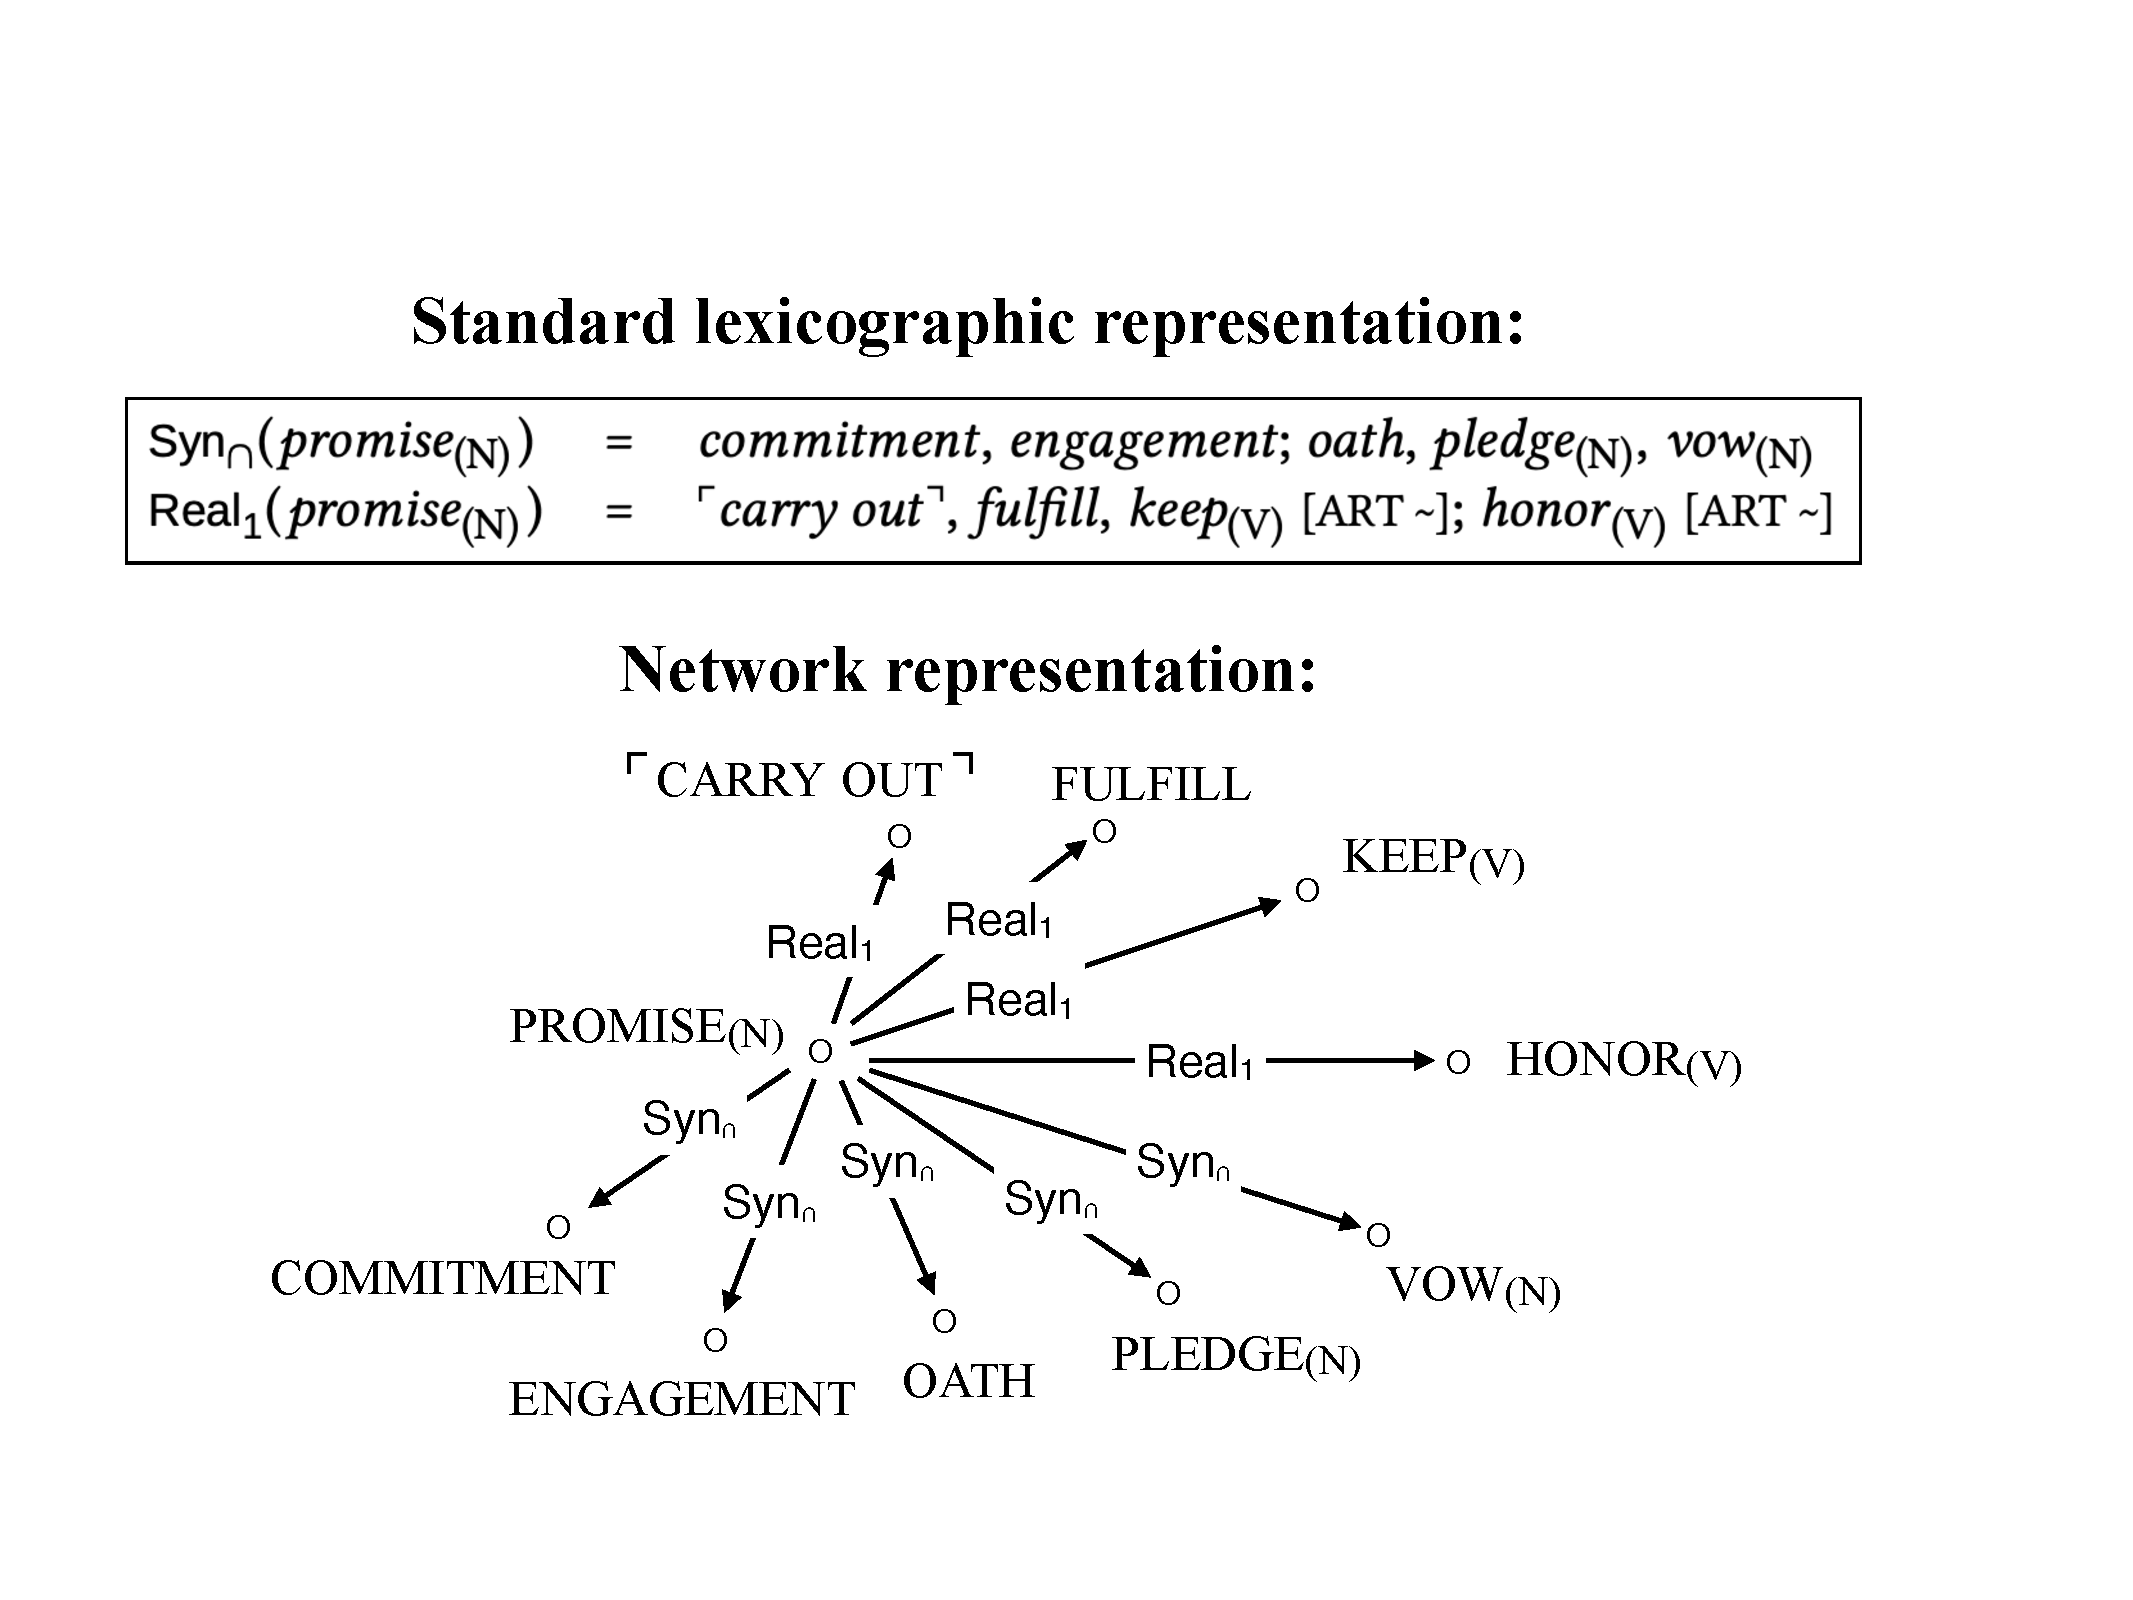
\includegraphics[width=9.5cm]{Fig/NotionLF/LFEquivLN-PROMISE.pdf}
\caption{Lexical network representing a set of LF applications}\label{fig:LFEquivLN-PROMISE}
\end{figure}\index[lf]{Syn@\lf{Syn}!\lf{Syn\tsub{$\cap$}}}\index[lf]{Reali@\lf{Real\tsub{i}}!\lf{Real\tsub{1}}}

%\begin{longtable*}[l]{ l l p{8cm} }
%\lfappl{Syn\tsub{$\cap$}}{\textit{promise}\tsub{(N)}} & = & \textit{commitment}\textbf{,} \textit{engagement}\textbf{;} \textit{oath}\textbf{,} \textit{pledge}\tsub{(N)}\textbf{,} \textit{vow}\tsub{(N)} \\
%\lfappl{Real\tsub{1}}{\textit{promise}\tsub{(N)}} & = & \idiom{\textit{carry out}}\textbf{,} \textit{fulfill}\textbf{,} \textit{keep}\tsub{(V)} \lfgp{\textsc{art} \tld}\textbf{;} \textit{honor}\tsub{(V)} \lfgp{\textsc{art} \tld} \\
%\end{longtable*}

The important issue of the structuring of lexical networks by LFs is considered in \chapref{chap:lexicalNetwork}.

\subsection{Notation for LF applications}\label{sec:notationForLFApplications}

Throughout this book, we use a set of notations\index[notion]{notation for LF application}\index[notion]{application of an LF}\index[notion]{lexical function!application of a \tld} (writing conventions and symbols) to present examples of LF applications. The general format of presentation for an LF application is as follows:

\begingroup
\small

\ex. \begingroup\setlength{\tabcolsep}{2pt}
\begin{tabular}[t]{ l l p{7cm} }
\lfappl{S\tsub{0}}{\textit{leave}\tsub{(V)}} & = & \textit{departure} \\
\end{tabular}\endgroup

\endgroup

The argument and the elements of the value of the LF are written in italics in the above formula -- though, technically, they are lexemes and should be written using the standard convention for lexical units: \textsc{leave}\tsub{(V)} and \textsc{departure}. However, this violation of conventions allows for easier legibility; additionally, values might not be lexical units (e.g., they can be collocations) and it is easier to use a uniform presentation for values, disregarding their lexical status. Note that lists of values in our examples are not necessarily complete; we often limit ourselves to only one value element.

As illustrated in example \Next, three symbols are used to separate the elements of an LF value: ``\textbf{,}'' for no or minimal semantic difference, ``\textbf{<}'' for the difference of degree, and ``\textbf{;}'' for a significant semantic difference.

\begingroup
\small

\ex. \begingroup\setlength{\tabcolsep}{2pt}
\begin{tabular}[t]{ l l >{\raggedright\arraybackslash}p{8cm} }
\lfappl{Magn}{\textit{salary}} & = & \textit{big}\textbf{,} \textit{generous}\textbf{,} \textit{hefty}\textbf{,} \textit{large}\textbf{,} \textit{substantial} \textbf{<} \textit{enormous}\textbf{,} \textit{huge}\textbf{,} \textit{massive}\textbf{;} \textit{exorbitant} \\*
\multicolumn{3}{>{\raggedright\arraybackslash}p{10cm}}{{\footnotesize [The value \textit{exorbitant} expresses an additional semanteme:  `too much'.]}} \\
\end{tabular}\endgroup

\endgroup

The ``\fused'' symbol used in \Next below indicates a fused\index[notion]{fusion}\index[notion]{value of an LF!fused \tld}\index[notion]{lexical function!fused value of a \tld} value element (see \sectref{sec:quidProQuoValues}, p.\thinspace\pageref{par:fusedValuesSyntLFs}).

\begingroup
\small

\ex. \begingroup\setlength{\tabcolsep}{2pt}
\begin{tabular}[t]{ l l >{\raggedright\arraybackslash}p{8cm} }
\lfappl{Magn}{\textit{amaze}} & = & \textit{utterly}\textbf{,} \fused\textit{stun}\tsub{(V)} {\footnotesize [$\equiv$ \textit{utterly amaze}]} \\
\end{tabular}\endgroup

\endgroup

Finally, two indications can follow a given value element L′.

\begin{enumerate}

\item \label{par:valueGP}The government pattern\index[notion]{government pattern!\tld\ of an LF value element|emph}\index[notion]{value of an LF!government pattern of an element of the \tld|emph}\footnote{On government patterns, see \chapref{chap:preliminaryNotions}, \sectref{sec:syntacticNotions}, p.\thinspace\pageref{txt:governmentPattern}.} of L′, written between square brackets, specifies the syntactic configuration that L′ can govern. This configuration is presented in simplified linear form; for instance in \Next below, where ``\tld'' stands for the LF's argument (\textit{kiss}\tsub{(N)}) and ``\textsc{art}'' stands for a determiner:

\begingroup
\small

\ex. \begingroup\setlength{\tabcolsep}{2pt}
\begin{tabular}[t]{ l l >{\raggedright\arraybackslash}p{8cm} }
\lfappl{Oper\tsub{1}}{\textit{kiss}\tsub{(N)}} & = & \textit{give} \lfgp{\textsc{art} \tld\ \textit{to} N\tsub{Y}} \\
\end{tabular}\endgroup

\endgroup

\item Semantic or grammatical constraints associated with L′ are introduced by a vertical bar ``\thinspace\constrbar\thinspace''; for instance:

\begingroup
\small

\ex. \begingroup\setlength{\tabcolsep}{2pt}
\begin{tabular}[t]{ l l >{\raggedright\arraybackslash}p{8cm} }
\lfappl{Oper\tsub{1}}{\textit{visit}\tsub{(N)}} & = & \textit{pay} \lfgp{\textsc{art} \tld\ \textit{to} N\tsub{Y}} \lfconstr{N\tsub{Y} denotes a person} \\
\end{tabular}\endgroup

\endgroup

\end{enumerate}

\section{Simple standard LFs}\label{sec:characStandardLFs}

The LFs as defined in \sectref{sec:LexMathFunctions} constitute a system\index[notion]{lexical function!system of standard \tlds}\index[notion]{system of standard LFs} built around a core of about seventy LFs, called \notion{simple standard LFs}\index[notion]{lexical function!standard \tld|emph}; they are referred to just as \textit{LFs} in the subsequent discussion. Let us present the fundamental properties of these LFs.

The set of LFs has been empirically identified over the last 60 years in the context of the study of typologically varied languages (first publication on LFs: \cite{ZolkovskijMelcuk1965-e}). The work on Russian and French Explanatory Combinatorial Dictionaries\index[notion]{dictionary!Explanatory Combinatorial \tld}\index[notion]{Explanatory Combinatorial!\tld\ Dictionary}\index[notion]{lexicography} has allowed the researchers to sharpen the LF system and to consolidate the very notion of LF, under the elaboration of lexical entries\index[notion]{lexical entry}, where LFs are systematically used \parencite{MelcukZholkovsky1984,MelcukZolkovskij2016,MelcukEtAl1984,MelcukEtAl1988,MelcukEtAl1992,MelcukEtAl1999,MelcukPolguere2007-e}. At the same time, Meaning-Text\index[notion]{Meaning-Text!\tld\ approach} research on \notion{syntactic paraphrasing}\index[notion]{paraphrase!syntactic \tld} \parencites{Milicevic2007}[Ch.~9]{Melcuk2013c-e} and dependency syntax\index[notion]{syntax!dependency \tld}\index[notion]{dependency!\tld\ syntax} \parencite{MelcukPertsov1987,Melcuk1988a,Melcuk2009a,Melcuk2015c,Melcuk2016b,Melcuk2021a} have heavily contributed to the maturation of the notion.

Three topics are discussed below: fundamental properties of LFs (\sectref{sec:FLStandard2Carac}), non-standard LFs (\sectref{par:nonStandardLFs}) and LFs in deep syntax (\sectref{sec:DSyntAndLFs}).

\subsection{Properties of simple standard LFs}\label{sec:FLStandard2Carac}

Simple standard LFs have two fundamental properties: a vast domain of application (\sectref{sec:vastDomainOfApplication}) and a vast range of possible values\index[notion]{value of an LF}\index[notion]{lexical function!value of a \tld} (\sectref{sec:vastRangeOfValues}). These properties follow from the character of the constrained meanings\index[notion]{meaning!constrained \tld} \sigmaF\ that simple standard LFs express.\footnote{On constrained meanings, see \sectref{sec:LFDefinitionNotion}, p.\thinspace\pageref{txt:constrainedMeaning}.}

The first property implies two other more specific properties: potential morphological expression of \sigmaF\ in natural languages (\sectref{sec:morphologicalExpressionSigmaF}) and universality of simple standard LFs (\sectref{sec:universality}).

\subsubsection{Vast domain of application}\label{sec:vastDomainOfApplication}

A given LF \lf{f} takes, in a given natural language, a large number of arguments: it has a vast domain of application\index[notion]{domain of application of an LF}\index[notion]{application of an LF!domain of \tld}\index[notion]{lexical function!domain of application of a \tld}. To put it differently, the meaning \sigmaF\ must be sufficiently vague (i.e., impoverished) to be compatible with a large set of lexical meanings to which it is supposed to be united\slashs{}associated.

Consequently, an \lf{f} involves a significant subset of a language's lexicon, and this subset is semantically rather heterogenous. Thus, for instance, one may wish to postulate a simple standard LF with meaning `young of L' to describe the following \notion{lexical relations}\index[notion]{lexical relation|emph}\index[notion]{relation!lexical \tld|emph}\phantomsection\label{txt:lexicalRelationIntro}:

\begingroup
\small

\ex. \begingroup\setlength{\tabcolsep}{2pt}
\begin{tabular}[t]{ l l l }
\textit{cat} & \lexRel{\lf{young of}} & \textit{kitten} \\
\textit{dog} & \lexRel{\lf{young of}} & \textit{puppy} \\*
\textit{pig} & \lexRel{\lf{young of}} & \textit{piglet} \\
\end{tabular}\endgroup\label{tab:youngOf}

\endgroup

This, however, would not be correct since this LF's meaning specifies a very constrained \notion{semantic class}\index[notion]{semantic!\tld\ class} of potential arguments: that of animate beings. Such a lexical relation can be described by an LF, but by a \emph{non-standard} LF\index[notion]{lexical function!non-standard \tld} (see \sectref{par:nonStandardLFs}, p.\thinspace\pageref{par:nonStandardLFs}).

\begin{soundboxnotitle}

A lexical relation \lf{LexRel} -- of any type -- between lexical units L and L′ is denoted as L\thinspace\lexRel{\lf{LexRel}}\thinspace L′.

\end{soundboxnotitle}

\subsubsection{Vast range of possible values}\label{sec:vastRangeOfValues}

The application \lfappl{f}{L} returns a large number of different values for different arguments: \lf{f} is, therefore, not a trivial relation. An LF that would express the meaning `of white color' would have a trivial value: \textsc{white}\tsub{(Adj)} for any lexical unit L. Such trivial cases must not be considered when identifying standard LFs.

\subsubsection{Potential morphological expression of \sigmaF}\label{sec:morphologicalExpressionSigmaF}

The first above property (vast domain of application) entails another significant property of standard LFs. Given their frequency in the language and their semantic regularity, one can expect the expression of \sigmaF\ by morphological means\index[notion]{morphology!morphological means}. This can happen, in a given language, either massively or sporadically; for instance:

\begin{itemize}

\item to implement the LF \lf{S\tsub{1}} (\chapref{chap:paraLFs}, [\ref{lf:S-i}], p.\thinspace\pageref{lf:S-i}), English uses the very productive derivational suffix\index[notion]{suffix!derivational \tld} \textsc{-er} (\textit{driv}+\textit{er}, \textit{advis}+\textit{er}, ...);

\item by contrast, one finds in French the unproductive nominal derivational suffix \mbox{\textsc{-aillon}} that expresses the complex LF \lf{AntiBon}\index[lf]{AntiBon@\lf{AntiBon}}\index[lf]{Bon@\lf{Bon}!AntiBon@\lf{AntiBon}} (\chapref{chap:syntLFs}, [\ref{lf:Bon}], p.\thinspace\pageref{lf:Bon}): {\smaller French}~\textit{avoc}+\textit{aillon} `bad lawyer' (from \textit{avocat} `lawyer'), \textit{écriv}+\textit{aillon} `bad writer' (from \textit{écrivain} `writer'), and a few other nouns.

\end{itemize}

\subsubsection{Universality of simple standard LFs}\label{sec:universality}

LFs that have the above properties are linguistically \notion{universal}\index[notion]{language-universal}; by this, we mean two things.

Firstly, each LF is supposed to be found in all or most world languages. We say \textit{most} because an LF can be trivial in a given language: it is always expressed there by the same linguistic means -- a given lexical unit or a given affix\index[notion]{affix}.

Secondly, the system of LFs proposed in the present volume is presumed complete. It is believed (until proven wrong) that one cannot find in a language a lexical relation with the above properties of simple standard lexical functions that would not be included in the proposed system.

Given\phantomsection\label{txt:LFNames} LFs' linguistic universality, it seems natural that their names\index[notion]{lexical function!\tld\ name} come from Latin, so that they are not linked to any specific contemporary language.\footnote{The LF \lf{Equip} (\chapref{chap:paraLFs}, [\ref{lf:Equip}], p.\thinspace\pageref{lf:Equip}), from {\smaller French}~\textit{équipage} `crew', is an exception.} To keep LF formulas relatively short, Latin sources are truncated to a maximum of four or five characters -- e.g., \lf{Syn}\index[lf]{Syn@\lf{Syn}}, from {\smaller Latin}~\textit{synonymum}. In a few cases, pseudo-Latin terms are used, preceded by an asterisk -- e.g., \lf{Conv\tsub{ijk}}\index[lf]{Convijk@\lf{Conv\tsub{ijk}}}, from {\smaller Latin}~*\textit{conversivum}.

\subsection{Non-standard LFs}\label{par:nonStandardLFs}\index[notion]{lexical function!non-standard \tld|emph}

Any natural language possesses an open set of constrained meanings\index[notion]{meaning!constrained \tld} \sigmaF\ such that:

\begin{itemize}

\item Each one of them is much richer than meanings of standard LFs.

\item Because of this, a \sigmaF\ can apply only to a semantically limited set of arguments; in point of fact, its domain of application\index[notion]{domain of application of an LF}\index[notion]{application of an LF!domain of \tld}\index[notion]{lexical function!domain of application of a \tld} is a clearly identifiable semantic field\index[notion]{semantic!\tld\ field} or a handful of lexical units. Quite frequently, its domain is even reduced to one lexical unit.

\item There is not much variability in its expression -- most of the time, just one lexical unit.

\end{itemize}

Such meanings are still expressed as a function of their argument and therefore they can be described by LFs, but by LFs of a completely different nature than standard LFs: these are \notion{non-standard LFs}.

Three examples are given in \Next: \lf{young of}, mentioned earlier in \ref{tab:youngOf}, which only applies to the semantic class\index[notion]{semantic!\tld\ class} of lexical units denoting higher-order animals; \lf{overprotective of their children}, which applies only to \textsc{parent}\tsub{(N)}, \textsc{mother}\tsub{(N)} and \textsc{father}\tsub{(N)} (and a few of their synonyms); \lf{of 366 days}, which applies only to the lexical unit \textsc{year}.

\begingroup
\small

\ex. \begingroup\setlength{\tabcolsep}{2pt}
\begin{tabular}[t]{ l l >{\raggedright\arraybackslash}p{6cm} }
\lfappl{young of}{\textit{cat}\tsub{(N)}} & = & \textit{kitten}\tsub{(N)} \\*
\lfappl{overprotective of her child}{\textit{mother}\tsub{(N)}} & = & \textit{helicopter}\tsub{(N)} \lfgp{\tld}  \\*
\lfappl{of 366 days}{\textit{year}} & = & \textit{leap}\tsub{(N)} \lfgp{\tld}  \\
\end{tabular}\endgroup

\endgroup

Non-standard LFs differ from standard LFs in the following aspects:

\begin{itemize}

\item They are not universal\index[notion]{language-universal}, but language-specific.

\item Their number in a given language is unlimited, and they cannot be theoretically foreseen.

\item They are so diverse that it is difficult to normalize them, and they have to be specified by the lexicographic definition\index[notion]{definition!lexicographic \tld} of their value.

\item Prototypically, they are not deep lexical units\index[notion]{lexical unit!deep \tld}: they do not appear in deep-syntactic structures\index[notion]{deep-syntactic!\tld\ structure [DSyntS]}\index[notion]{structure!deep-syntactic \tld\ [DSyntS]} and do not participate in universal paraphrasing\index[notion]{paraphrase}, unlike standard LFs -- see \sectref{sec:DSyntAndLFs} below. Their only job is to ensure correct lexical selection\index[notion]{lexical access\slashs{}selection} in the transition from the semantic\index[notion]{structure!semantic \tld\ [SemS]}\index[notion]{semantic!\tld\ structure [SemS]} to the deep-syntactic structure.

\end{itemize}

\begin{furtherreading}
On standard vs. non-standard LFs, see \textcite{Polguere2007a-e} and \textcite[Appendix]{Melcuk2023a}.
\end{furtherreading}

\subsection{Standard LFs in deep syntax}\label{sec:DSyntAndLFs}\index[notion]{syntax!deep \tld}

\subsubsection{LFs as deep lexical units}\label{sec:LFAsDeepLU}

An application\index[notion]{application of an LF}\index[notion]{lexical function!application of a \tld} \lfappl{f}{L} specifies a set of alternative lexical units: it is, so to speak, a meta-unit. It appears in the deep-syntactic structure [DSyntS]\index[notion]{structure!deep-syntactic \tld\ [DSyntS]}\index[notion]{deep-syntactic!\tld\ structure [DSyntS]} of a sentence, to be replaced by a specific lexical unit selected for the surface-syntactic structure [SSyntS]\index[notion]{structure!surface-syntactic \tld\ [SSyntS]}\index[notion]{surface-syntactic!\tld\ structure [SSyntS]}. As such, an application \lfappl{f}{L} is a deep lexical unit\index[notion]{lexical unit!deep \tld}. This is illustrated by \figref{fig:LFDSyntStruct}.

\begin{quote}

\remark{Reminder.}For the semantic and syntactic notions used in the present section -- as well as for the representation of semantic and syntactic structures, see \chapref{chap:preliminaryNotions}, Sections~\ref{sec:semanticNotions} and~\ref{sec:syntacticNotions}.

\end{quote}

\begin{figure}

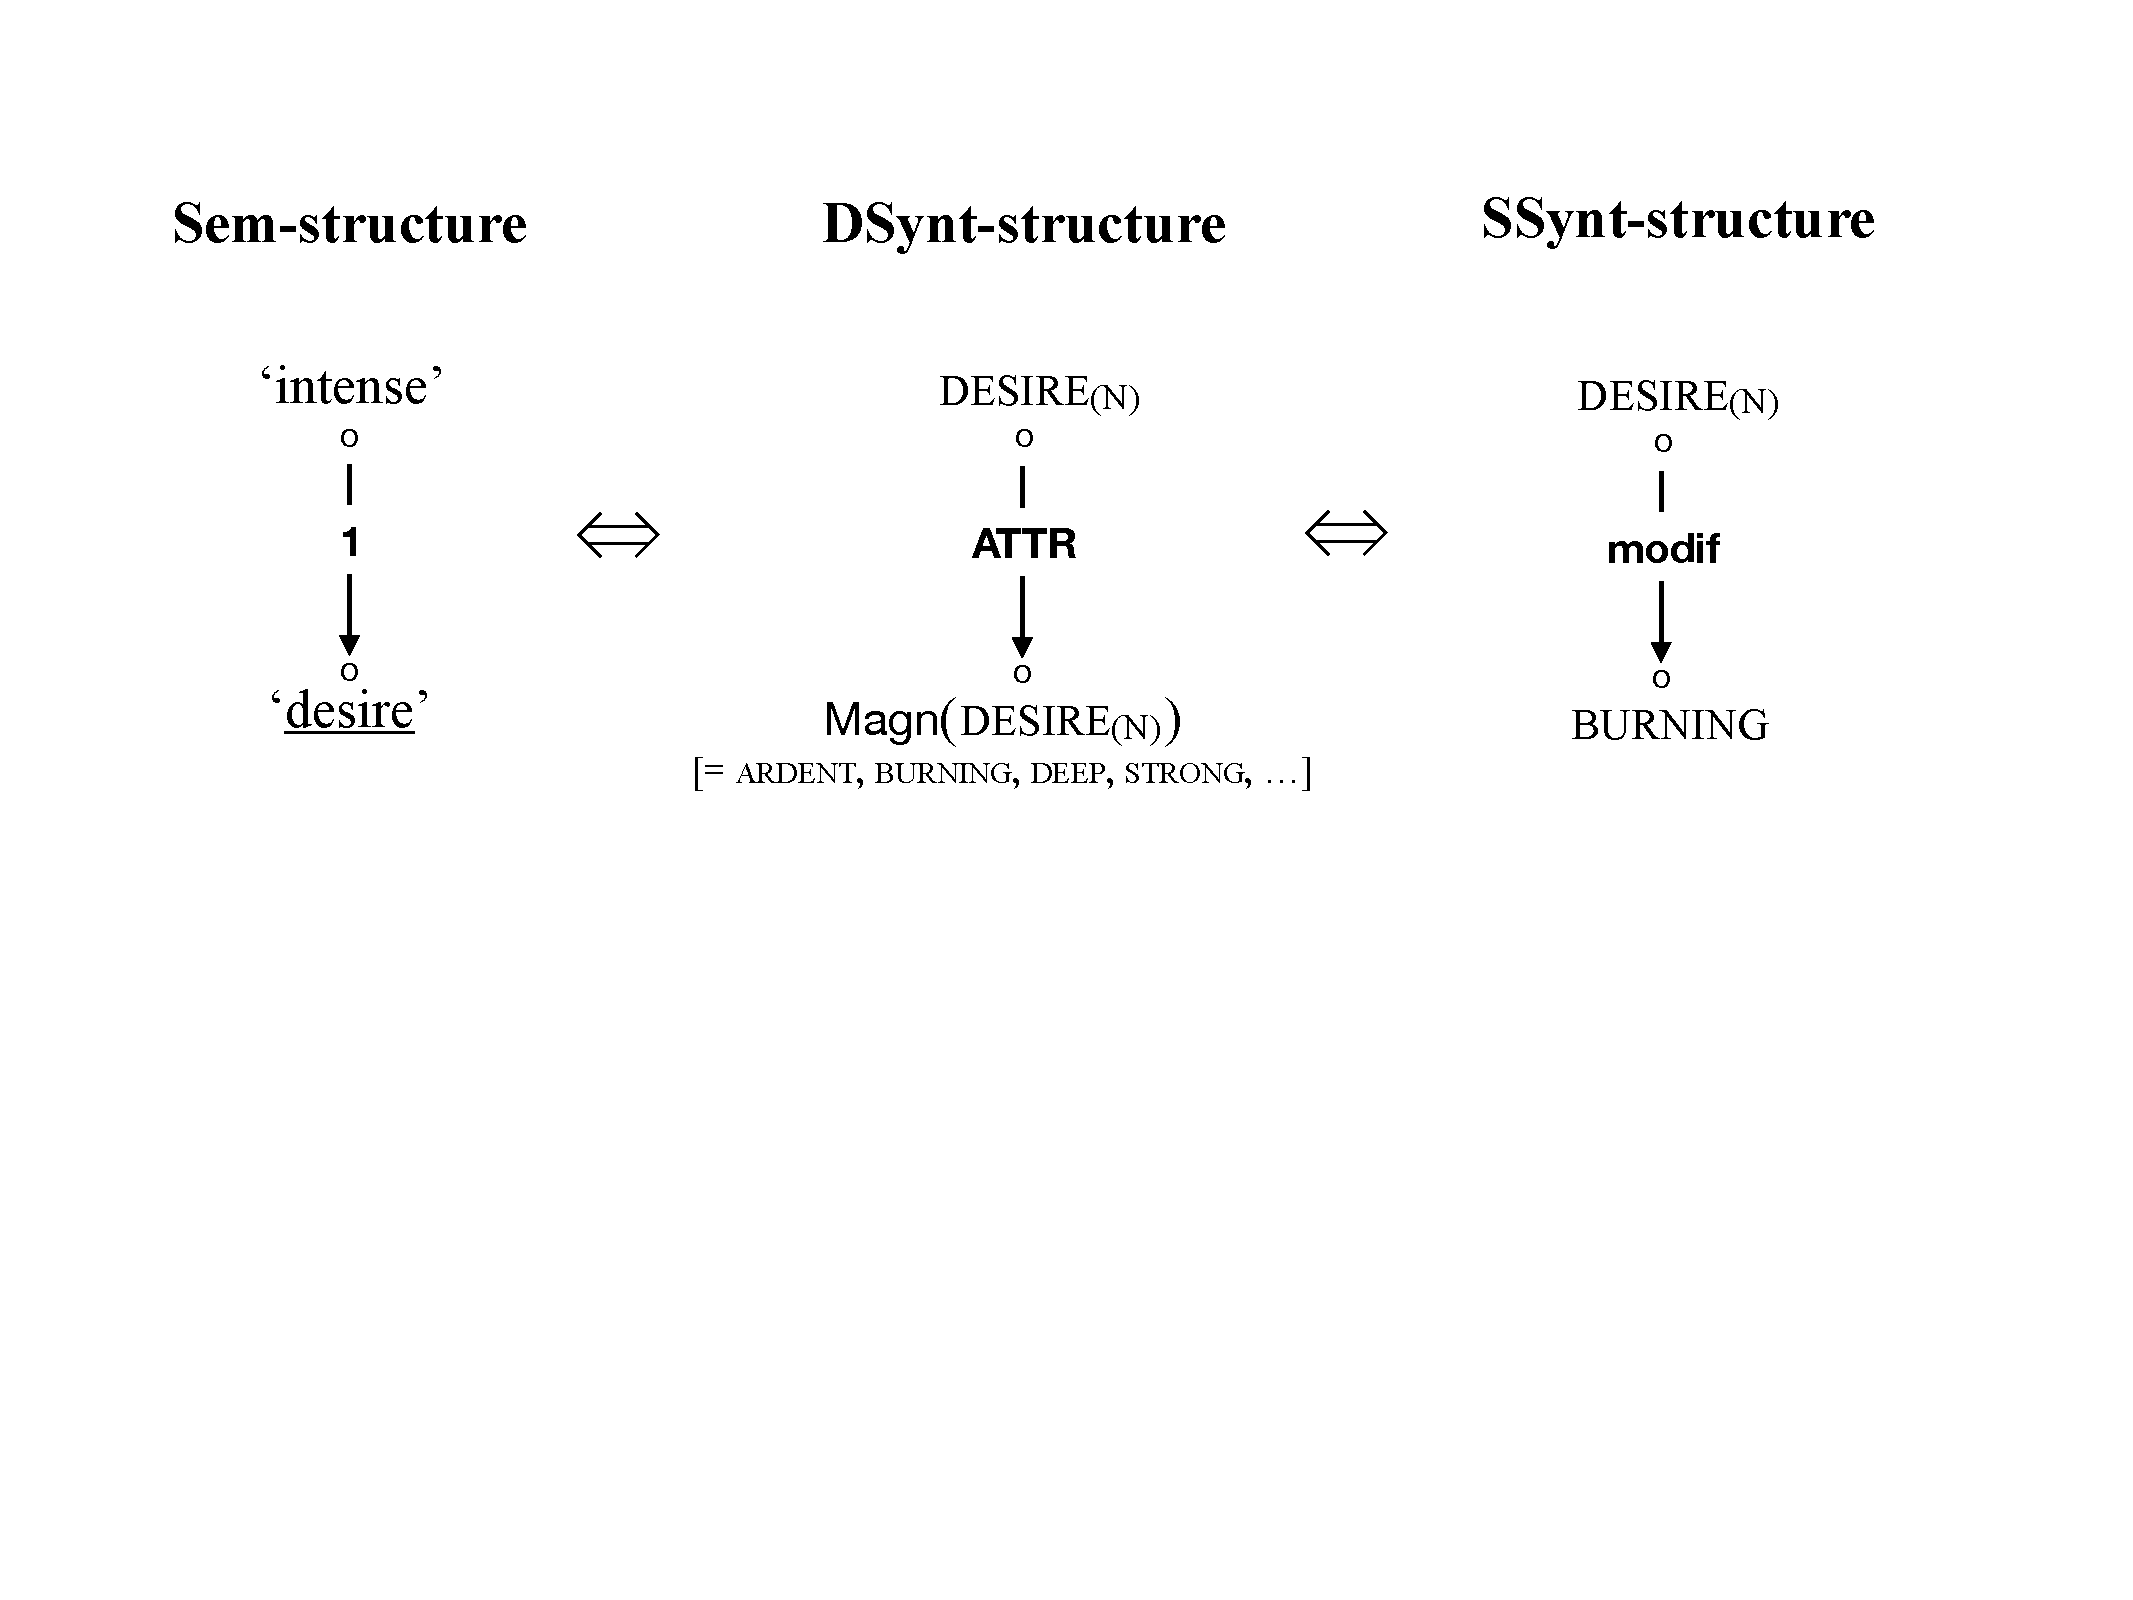
\includegraphics[width=12cm]{Fig/NotionLF/LFDSyntStruct.pdf}
\caption{\lf{Magn} in the DSyntS of the phrase \textit{burning desire}}\label{fig:LFDSyntStruct}
\end{figure}

\figref{fig:LFDSyntStruct} shows as well that, in linguistic representations, LFs appear only in DSyntSs. Being a lexical element in DSyntS, an LF has its own combinatorial properties, in particular, a deep part of speech\index[notion]{part of speech [PoS]!deep \tld} (see \sectref{sec:PofS}, p.\thinspace\pageref{sec:PofS}).

LFs fulfill two tasks in deep syntax: correct lexical selection (\sectref{sec:LFAndLexicalization}) and DSynt-paraphrasing (\sectref{sec:LFStandardParaphrasing}).

\subsubsection{LFs and lexical selection}\label{sec:LFAndLexicalization}

\notion{Lexical selection}\index[notion]{lexical selection|emph} is an important part of what is known as \notion{lexicalization}\index[notion]{lexicalization (in speech production)|emph} in speech production\index[notion]{speech!\tld\ production} -- e.g., in psycholinguistics\index[notion]{psycholinguistics} research \parencite{KempenHuijbers1983} and in computer text generation \parencite{Stede1994}.

Under lexical selection\index[notion]{lexical access\slashs{}selection}, LFs ensure correct choices in case a lexical unit has to be selected contingent upon another lexical unit in the same utterance.

Thus, \figref{fig:LFDSyntStruct} above represents the following steps in lexicalization:

\begin{enumerate}

\item At the Sem-level, the semanteme `intense' is identified as a constrained meaning\index[notion]{meaning!constrained \tld} (\sectref{sec:LFDefinitionNotion}, p.\thinspace\pageref{txt:constrainedMeaning}), to be lexically expressed as function of the expression of the semanteme `desire'.

\item At the DSynt-level, the semanteme `intense' is expressed by (the name of) the LF \lf{Magn}. This LF is applied to the lexeme \textsc{desire}\tsub{(N)}: the application \lfappl{Magn}{\textsc{desire}\tsub{(N)}} represents a constrained lexical choice, more precisely, a set of the usable syntactic modifiers of \textsc{desire}\tsub{(N)}, which express the semanteme `intense'.

\item At the SSynt-level, the lexical selection is completed: the lexeme \textsc{burning} is introduced as a modifier of \textsc{desire}\tsub{(N)}; this is done on the basis of the lexical entry\index[notion]{lexical entry} of \textsc{desire}\tsub{(N)}, where the value of the application \lfappl{Magn}{\textsc{desire}\tsub{(N)}} is specified.

\end{enumerate}

\subsubsection{LFs and paraphrasing}\label{sec:LFStandardParaphrasing}

A vital feature of natural languages is their ability to express, in a general case, a given meaning by a large set of quasi-synonymous utterances, i.e., \notion{paraphrases}\index[notion]{paraphrase|emph}, as shown in \figref{fig:paraphPotential}.

\begin{figure}

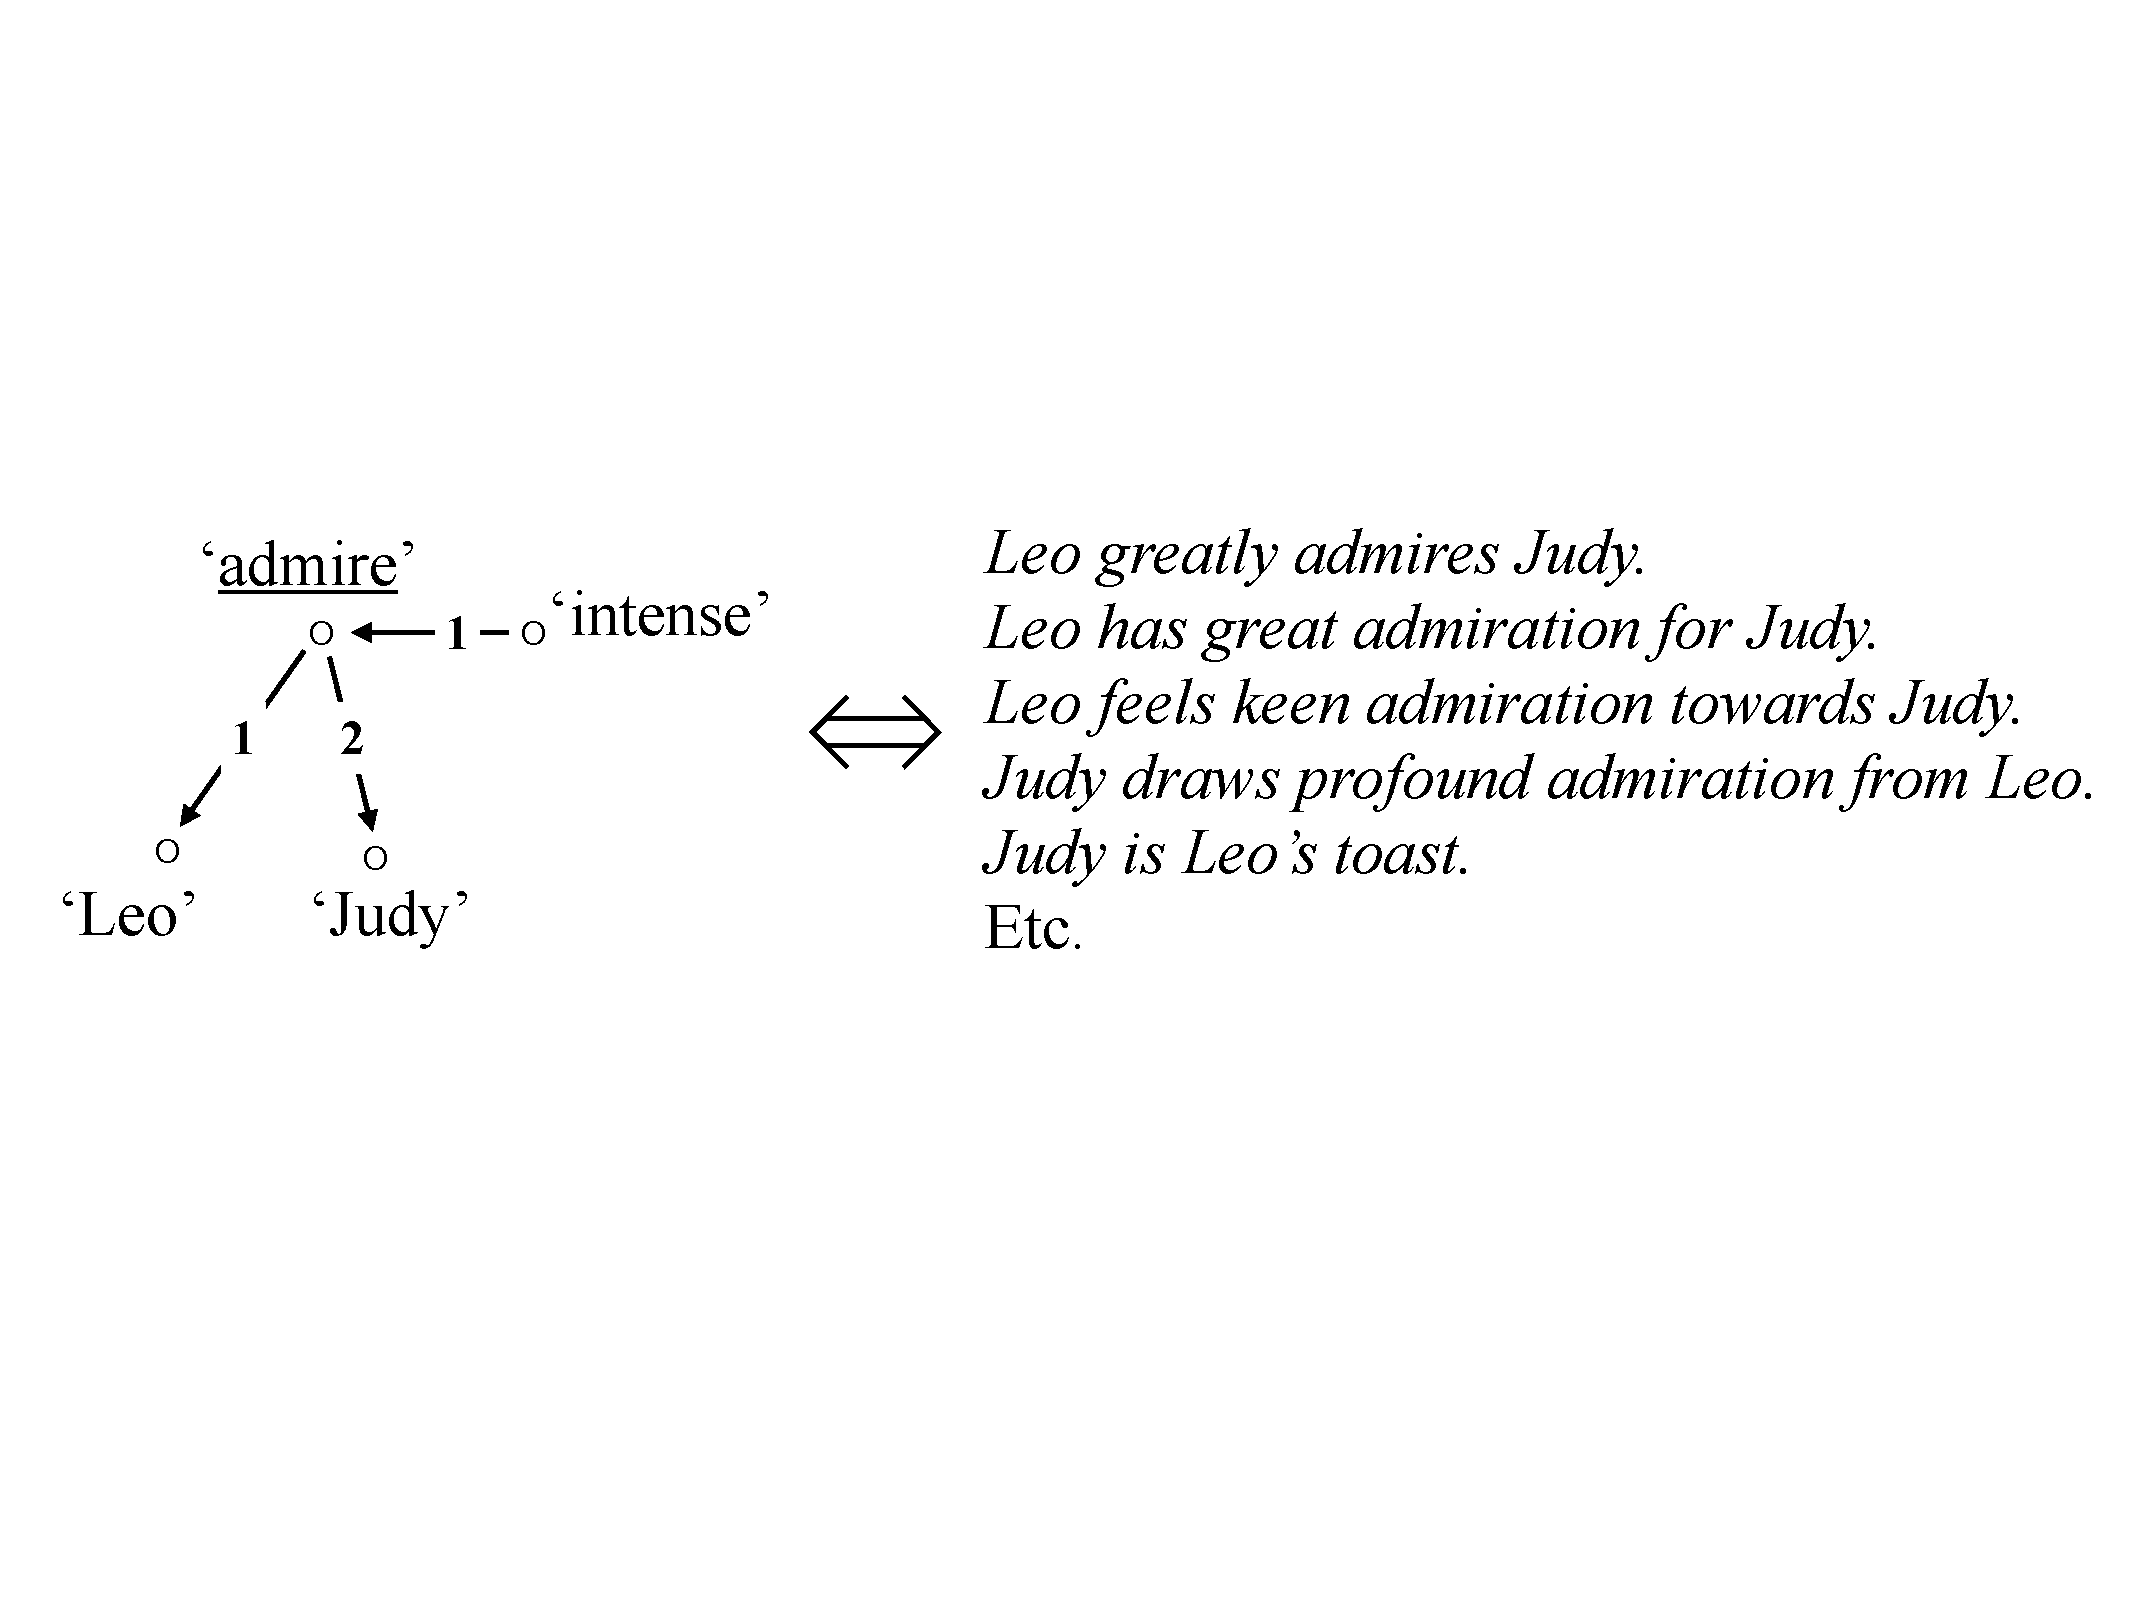
\includegraphics[width=11cm]{Fig/NotionLF/ParaphrasesIllustr.pdf}
\caption{Paraphrasing potential of a natural language}\label{fig:paraphPotential}
\end{figure}

This is but a modest illustration of what a natural language can do with regard to paraphrasing: a natural language is a paraphrasing device \parencite[Ch.~2]{Melcuk2012a-e}. Paraphrasing as such is not often used in actual speech production\index[notion]{speech!\tld\ production} -- only in specific situations: editing a text, rephrasing for better explanation, etc. However, the paraphrasing power\index[notion]{paraphrase!paraphrasing power of languages} of a language offers, at any given stage of speech production\index[notion]{speech!\tld\ production}, multiple alternatives that enable the Speaker\index[notion]{Speaker, the} to speak fluently. When speaking a second language, a person generally doesn't master the same paraphrasing wealth and therefore production can be slowed down or outright blocked.

The system of standard LFs\index[notion]{lexical function!system of standard \tlds}\index[notion]{system of standard LFs} plays a core role in the use of language, because it is in terms of LFs that \notion{deep-syntactic paraphrasing rules}\index[notion]{paraphrase!deep-syntactic paraphrasing rule|emph} are formulated. Since LFs are language-universal\index[notion]{language-universal} (see above, p.\thinspace\pageref{sec:universality}), the resulting system of paraphrasing rules is also universal. Such a paraphrasing system is described in \textcite[141--176]{Melcuk1974}, \textcite[Ch.~6]{Milicevic2007} and \textcite[Ch.~9]{Melcuk2013c-e}. Here, we limit ourselves to citing two paraphrasing rules: \textbf{R\tsub{\lf{Mult}}} and \textbf{R\tsub{\lf{Oper$_\text{1}$}}}.

\begin{center}
\APolbox{4.8cm}{%
\textbf{R\tsub{\lf{Mult}}:}\quad L\tsub{(N)\textsc{pl}}\enskip{\small $\equiv$}\enskip\lfappl{Mult}{L\tsub{(N)}}\tsub{\textsc{sg}}
}
\end{center}\phantomsection\label{txt:RParaphMult}\index[notion]{paraphrase!deep-syntactic paraphrasing rule!\textbf{R\tsub{\lf{Mult}}}|emph}\index[lf]{Mult@\lf{Mult}}

This rule describes the universal semantic equivalence between a plural noun L\tsub{(N)\textsc{pl}} and the corresponding collective noun \lfappl{Mult}{L} -- \chapref{chap:paraLFs}, [\ref{lf:Mult}], p.\thinspace\pageref{lf:Mult}; for instance:

\begingroup
\small

\ex. \begin{tabular}[t]{l c l}
     \textit{workers} & {\footnotesize $\cong$} & \textit{workforce} \\
     \textit{lies} & {\footnotesize $\cong$} & \textit{bunch of lies} \\
     \end{tabular}

\endgroup

Note that such equivalences hold for a specific meaning of the nominal plural: `collective of \lfgp{Ns}'. \lfappl{Mult}{L} itself is in the singular, as stated in the rule \textbf{R\tsub{\lf{Mult}}}.

\begin{center}
\APolbox{7.2cm}{%
\textbf{R\tsub{\lf{Oper$_\text{1}$}}:} L\tsub{(V)}\enskip{\small $\equiv$}\enskip\lfappl{Oper\tsub{1}}{\lfappl{S\tsub{0}}{L\tsub{(V)}}}\thinspace\syntRel{II}\thinspace\lfappl{S\tsub{0}}{L\tsub{(V)}}
}
\end{center}\phantomsection\label{txt:RParaphOper1}\index[notion]{paraphrase!deep-syntactic paraphrasing rule!\textbf{R\tsub{\lf{Oper$_\text{1}$}}}|emph}\index[lf]{S0@\lf{S\tsub{0}}}\index[lf]{Operi@\lf{Oper\tsub{i}}!\lf{Oper\tsub{1}}}

This rule describes the universal semantic equivalence between a verb L\tsub{(V)} and the verbal collocation consisting of (i)~the \lf{S\tsub{0}} nominalization of L\tsub{(V)} (\chapref{chap:paraLFs}, [\ref{lf:S0}], p.\thinspace\pageref{lf:S0}) and (ii)~an \lf{Oper\tsub{1}} support verb of this nominalization (\chapref{chap:syntLFs}, [\ref{lf:Oper-i}], p.\thinspace\pageref{lf:Oper-i}). For instance:

\begingroup
\small

\ex. Leo \emph{admires} Judy.\enskip{\footnotesize $\equiv$}\enskip Leo \emph{has admiration} for Judy.

\endgroup

\subsubsection{Actantial subscripts in simple standard LFs}\label{sec:actSubsSimpleLF}

Actantial subscripts\index[notion]{actantial subscript|emph} to LF names have frequently appeared in the preceding text. An explanation of their interpretation is supplied here for the names of simple standard LFs. The corresponding explanation concerning the names of LFs in combinations\index[notion]{lexical function!\tld\ combination} is provided in \sectref{sec:actSubsLFCombinations} (p.\thinspace\pageref{sec:actSubsLFCombinations}).

In the general case of an application \lfappl{f\tsub{i}}{L} where \lf{f\tsub{i}} is a simple LF, the subscript ``\tsub{\lf{i}}'' refers to the DSyntA\thinspace\syntDname{i} of L. Here are two illustrations, with LFs \lf{S\tsub{2}}\index[lf]{Si@\lf{S\tsub{i}}!\lf{S\tsub{2}}} (\chapref{chap:paraLFs}, [\ref{lf:S-i}], p.\thinspace\pageref{lf:S-i}) and \lf{Func\tsub{3}}\index[lf]{Funci@\lf{Func\tsub{i}}!\lf{Func\tsub{3}}} (\chapref{chap:syntLFs}, [\ref{lf:Func-i}], p.\thinspace\pageref{lf:Func-i}).

\begingroup
\small

\ex. \a. \begingroup\setlength{\tabcolsep}{2pt}
\begin{tabular}[t]{ l l l }
\lfappl{S\tsub{\textbf{2}}}{\textit{eat} \lfgp{`X eats \textbf{Y}'}} & = & \textit{food} \\
\end{tabular}\endgroup
      \b. \begingroup\setlength{\tabcolsep}{2pt}
\begin{tabular}[t]{ l l l }
\lfappl{Func\tsub{\textbf{3}}}{\textit{ultimatum} \lfgp{`X's ultimatum to Y to do \textbf{Z} before time T'}} & = & \textit{call}\tsub{(V)} \lfgp{\textit{for} N\tsub{Z}} \\
\multicolumn{3}{l}{Ex.: \textit{The ultimatum calls}\tsub{\lfappl{Func$_\text{3}$}{\textit{ultimatum}}} \textit{for the release}\tsub{Z} \textit{of prisoners.}} \\
\end{tabular}\endgroup

\endgroup

However, there are at least three special cases of LFs where the interpretation of actantial subscripts is not straightforward:
 
 \begin{itemize}
 
 \item \lf{Adv\tsub{(i)}}\index[lf]{Advi@\lf{Adv\tsub{i}}!\lf{Adv\tsub{(i)}}}, which stands for absolutive adverbials\index[notion]{adverb!absolutive \tld ial} (such as \textit{in the presence of}) -- see \chapref{chap:paraLFs}, [\ref{lf:Adv-i}], Comment~2, p.\thinspace\pageref{para:comment2Advi};
 
 \item \lf{Sympt\tsub{ijk}}\index[lf]{Symptijk@\lf{Sympt\tsub{ijk}}}, which describes somatic phrasemes\index[notion]{phraseme!somatic \tld} of psychological or physiological states -- see \chapref{chap:syntLFs}, [\ref{lf:Sympt-ijk}], p.\thinspace\pageref{lf:Sympt-ijk};

\item \lf{Caus}\index[lf]{Caus@\lf{Caus}}, \lf{Liqu}\index[lf]{Liqu@\lf{Liqu}} and \lf{Perm}\index[lf]{Perm@\lf{Perm}}, which stand for verbs of causing\index[notion]{lexical function!\tld\ of causing} -- see \chapref{chap:syntLFs}, \sectref{sec:collocCausatif}.
 
 \end{itemize}

\section{Two major classes of simple standard LFs}\label{sec:LFParaSynt}\index[notion]{lexical function!paradigmatic vs. syntagmatic \tlds|emph}

LFs are divided in two classes, based on the two functional axes of natural languages \parencite[Part~2, Ch.~V]{Saussure1972}:

\begin{itemize}

\item the \notion{paradigmatic axis}\index[notion]{paradigmatic!\tld\ axis}, on which the Speaker\index[notion]{Speaker, the} performs the \emph{selection} of linguistic units to be used;

\item the \notion{syntagmatic axis}\index[notion]{syntagmatic!\tld\ axis}, on which the Speaker performs the \emph{combination} of selected linguistic units into higher-level units.

\end{itemize}

These two axes and the corresponding linguistic operations (selection vs. combination) determine the two classes of LFs: paradigmatic LFs (\sectref{sec:classeFLParadigmatiques}) and syntagmatic LFs (\sectref{sec:classeFLSyntagmatiques}).%\footnote{In the process of text production the operations of selection and combination intermingle: a particular selection of a linguistic unit specifies the conditions for eventual combinations, and a particular combination can require an alternative selection.}

\subsection{Paradigmatic LFs}\label{sec:classeFLParadigmatiques}

The application\index[notion]{application of an LF}\index[notion]{lexical function!application of a \tld} of a \notion{paradigmatic LF}\index[notion]{lexical function!paradigmatic \tld|emph}\index[notion]{paradigmatic!\tld\ lexical function|emph} to a lexical unit L returns as value\index[notion]{lexical function!value of a \tld}\index[notion]{value of an LF} a set of lexical entities of which each element L′ stands in a particular paradigmatic relation to L -- i.e., L′ is a possible substitute for L in the text. More precisely, L′ is a \notion{semantic derivative}\index[notion]{derivative!semantic \tld|emph}\index[notion]{semantic!\tld\ derivative|emph} of L. 

\phantomsection\label{def:semanticDerivative}\begin{notiondefinition}{semantic derivative}
A \notion{semantic derivative} of lexical unit L is a lexical entity L′ whose meaning `L′' includes `L' such that \\*[2pt]
\setlength{\tabcolsep}{.5pt}\begin{tabular}{ p{0.2cm} >{\raggedright\arraybackslash}p{11.1cm} }
\SpecDiff & the semantic difference `$\sigma$' $=$ `L′\verythinspace\textminus\verythinspace L' is found in a large enough number of lexical pairs of the language -- i.e., `$\sigma$' is regular\index[notion]{regularity}; \\
\SpecDiff & the language has dedicated means for expressing `$\sigma$' -- e.g., morphological means. \\[3pt]
\end{tabular}

\noindent
L is called the \notion{base of the derivative} L′.
\end{notiondefinition}\index[notion]{base!\tld\ of a derivative}\index[notion]{derivative!base of a \tld}\index[notion]{morphology!morphological means}

As anticipated by the above definition, there is a particular case of semantic derivative: \notion{morphological derivative}\index[notion]{derivative!morphological \tld}\index[notion]{morphology!morphological derivative}.

\begin{notiondefinition}{morphological derivative}
A \notion{morphological derivative} of lexical unit L is a semantic derivative L′ of L such that \\*[2pt]
\setlength{\tabcolsep}{.5pt}\begin{tabular}{ p{0.2cm} >{\raggedright\arraybackslash}p{11.1cm} }
\SpecDiff & the semantic difference `L′\verythinspace\textminus\verythinspace L' is expressed by a morphological means. \\
\end{tabular}
\end{notiondefinition}\index[notion]{morphology!morphological means}

A typical case of derivatives is that of \notion{Agent noun}\index[notion]{Agent (semantic role)!\tld\ noun}\index[notion]{semantic!\tld\ role}, or more precisely, the name for the first semantic actant\index[notion]{actant!semantic \tld\ [SemA]}\index[notion]{semantic!\tld\ actant [SemA]} [SemA~\syntDname{1}] `X' of L. Here are a few illustrations:

\begingroup
\small

\ex.\label{ex:illustrationsAgent} \begingroup\setlength{\tabcolsep}{2pt}
\begin{tabular}[t]{ l l >{\raggedright\arraybackslash}p{7.5cm} }
\textit{support}\tsub{(V)} & \lexRel{\lf{Agent noun}} & \textit{supporter} {\footnotesize `X who supports'} \\
\textit{agression} & \lexRel{\lf{Agent noun}} & \textit{agressor} {\footnotesize `X who commits an agression'} \\
\textit{congress} & \lexRel{\lf{Agent noun}} & \textit{congressman}\slashs\textit{congresswoman} {\footnotesize `X who is a member of a country's congress'} \\
\textit{boring} & \lexRel{\lf{Agent noun}} & \textit{bore}\tsub{(N)} {\footnotesize `X who is boring'} \senseex{He is an awful bore.} \\
\textit{account}\tsub{(N)} & \lexRel{\lf{Agent noun}} & \textit{account holder} {\footnotesize `X who has a bank account'} \\
\textit{steal}\tsub{(V)} & \lexRel{\lf{Agent noun}} & \textit{thief} {\footnotesize `X who steals'} \\
\textit{annoying} & \lexRel{\lf{Agent noun}} & \uslabel{vulgar} \idiom{\textit{pain in the ass}} {\footnotesize `X that is annoying'} \\*
\textit{heal} & \lexRel{\lf{Agent noun}} & \textit{remedy}\tsub{(N)} {\footnotesize `X that heals'} \\
\end{tabular}\endgroup

\endgroup

Among these semantic derivatives, the first four are also morphological derivatives\index[notion]{derivative!morphological \tld}\index[notion]{morphology!morphological derivative}.

Semantic derivation is described by paradigmatic LFs in the following way:

\begin{itemize}

\item a given paradigmatic LF \lf{f} specifies a particular family of semantic derivatives that express the meaning \sigmaF;

\item it takes as arguments the bases of derivatives;

\item it returns as values the derivatives themselves.

\end{itemize}

For instance, the semantic derivation of Agent\index[notion]{Agent (semantic role)}\index[notion]{semantic!\tld\ role} nouns mentioned above is described by the paradigmatic LF \lf{S\tsub{1}}\index[lf]{Si@\lf{S\tsub{i}}!\lf{S\tsub{1}}} with the meaning `somebody who\slashs{}something that ...' (\chapref{chap:paraLFs}, [\ref{lf:S-i}], p.\thinspace\pageref{lf:S-i}). For  the illustrations \ref{ex:illustrationsAgent}, it is encoded as in \ref{ex:illustrationsAgentEncoding}:

\begingroup
\small

\ex.\label{ex:illustrationsAgentEncoding} \begingroup\setlength{\tabcolsep}{2pt}
\begin{tabular}[t]{ l l >{\raggedright\arraybackslash}p{7cm} }
\lfappl{S\tsub{1}}{\textit{support}\tsub{(V)}} & = & \textit{supporter} \\
\lfappl{S\tsub{1}}{\textit{agression}} & = & \textit{agressor} \\
\lfappl{S\tsub{1}}{\textit{congress}} & = & \textit{congressman}\textbf{,} \textit{congresswoman} \\
\multicolumn{3}{ l }{etc.} \\
\end{tabular}\endgroup

\endgroup

\paragraph*{Remark on the LF \lf{Syn}.}\label{par:remarkOnSyn}

The LF \lf{Syn}\index[lf]{Syn@\lf{Syn}} `synonym' (\chapref{chap:paraLFs}, [\ref{lf:Syn}], p.\thinspace\pageref{lf:Syn}) occupies a special place among paradigmatic LFs. It models a particular case of the most important relation underlying the functioning of natural languages: \notion{synonymy in the broad sense}\index[notion]{synonymy!\tld\ in the broad sense}, i.e., semantic equivalence between linguistic expressions. Consequently, \lf{Syn} underlies the simplest paraphrasing rule\index[notion]{paraphrase!deep-syntactic paraphrasing rule}:

\begin{center}
\APolbox{3.3cm}{%
\textbf{R\tsub{\lf{Syn}}:}\quad L\enskip{\small $\equiv$}\enskip\lfappl{Syn}{L}\label{ex:regleParaphrasageSyn}
}
\end{center}\label{txt:RSyn}\index[notion]{paraphrase!deep-syntactic paraphrasing rule!\textbf{R\tsub{\lf{Syn}}}|emph}

Note that all paraphrasing rules -- e.g., rules \textbf{R\tsub{Mult}}\index[notion]{paraphrase!deep-syntactic paraphrasing rule!\textbf{R\tsub{\lf{Mult}}}} and \textbf{R\tsub{\lf{Oper$_\text{1}$}}}\index[notion]{paraphrase!deep-syntactic paraphrasing rule!\textbf{R\tsub{\lf{Oper$_\text{1}$}}}} (\sectref{sec:LFStandardParaphrasing}, p.\thinspace\pageref{txt:RParaphMult}) -- establish the synonymy\index[notion]{synonymy} relations between linguistic expressions. Even more importantly, the Meaning-Text approach\index[notion]{Meaning-Text!\tld\ approach} is built on the notion of \notion{Meaning}\index[notion]{meaning!Meaning \lfgp{with a capital \textit{M}}} (written with a capital \textit{M}), which is the invariant of a set of paraphrases, i.e., synonymous expressions \parencites[10--11]{Melcuk1974}[44--45]{Melcuk2012a-e}[102--103]{MelcukMilicevic2014a}.

\subsection{Syntagmatic LFs}\label{sec:classeFLSyntagmatiques}

The application\index[notion]{application of an LF}\index[notion]{lexical function!application of a \tld} of a \notion{syntagmatic LF}\index[notion]{lexical function!syntagmatic \tld|emph}\index[notion]{syntagmatic!\tld\ lexical function|emph} to a lexical unit L\tsub{1} returns as value a set of lexical entities of which each element L\tsub{2} stands in a particular syntagmatic (i.e., cooccurrence\index[notion]{cooccurrence, restricted}) relation with L\tsub{1}. More precisely, L\tsub{2} forms a \notion{collocation}\index[notion]{collocation|emph} with L\tsub{1}.\footnote{\phantomsection\label{fn:NatureCollocates}The following definition would necessitate fine-tuning. In practice, instances of some sort of double-shot collocations can be found, where the collocate L\tsub{2} is not a lexical unit but is itself a collocation. For instance, the phraseme \textit{under the effect of alcohol} has all appearances of being a double-shot collocation, where \textsc{alcohol} is the base and \textit{under the effect} is itself a collocation with \textsc{effect}\tsub{(N)} as its base. For a description of \textit{under the effect} in terms of the LF \lf{A\tsub{2}}, see \chapref{chap:paraLFs}, [\ref{lf:A-i}], p.\thinspace\pageref{txt:A2UnderTheEffect}; for a description of \textit{under the effect of alcohol} in terms of the LF \lf{Propt\tsub{1}}, see \chapref{chap:syntLFs}, [\ref{lf:Propt-i}], p.\thinspace\pageref{txt:Propt1UnderTheEffectOfAlcohol}. Note that the LF \lf{Sympt\tsub{ijk}} is often used to encode phrasemes that seem like double-shot collocations -- see \chapref{chap:syntLFs}, [\ref{lf:Sympt-ijk}], p.\thinspace\pageref{lf:Sympt-ijk}.}\index[notion]{collocation!double-shot \tld|emph}\index[lf]{Ai@\lf{A\tsub{i}}!\lf{A\tsub{2}}}\index[lf]{Propti@\lf{Propt\tsub{i}}!\lf{Propt\tsub{1}}}\index[lf]{Symptijk@\lf{Sympt\tsub{ijk}}}

\phantomsection\label{def:collocation}\begin{notiondefinition}{collocation}
A \notion{collocation} is a compositional phraseme\index[notion]{phraseme} consisting, prototypically, of two lexical units L\tsub{1} and L\tsub{2} such that \\*
\setlength{\tabcolsep}{.5pt}\begin{tabular}{ p{0.2cm} >{\raggedright\arraybackslash}p{11cm} }
\SpecDiff & L\tsub{1} is selected by the Speaker\index[notion]{Speaker, the} freely, i.e., independently of any other lexical choice; \\
\SpecDiff & L\tsub{2} is selected by the Speaker to express a particular meaning \sigmaF\ in combination with L\tsub{1} as a function of L\tsub{1}. \\[3pt]
\multicolumn{2}{l}{L\tsub{1} is called the \notion{base of the collocation} and L\tsub{2}, its \notion{collocate}.} \\[3pt]
\end{tabular}

\noindent
\remark{Examples.}In the collocation \textit{deep feeling}, \textit{feeling} is the base and \textit{deep}, the collocate; in \textit{pay a visit}, \textit{visit} is the base and \textit{pay}, the collocate.
\end{notiondefinition}\index[notion]{base!\tld\ of a collocation|emph}\index[notion]{collocation!base of a \tld|emph}\index[notion]{collocation!collocate of a \tld|emph}

An emblematic case of collocation is that of intensification; here are three examples where collocates are italicized:

\begingroup
\small

\ex.\label{ex:collocationIntensification} \a. \emph{nagging} doubt
     \b. Thanks \emph{a million}!
     \c. drink \emph{\idiom{like a sponge}}

\endgroup

Syntagmatic LFs take as arguments lexical units that are bases of collocations and return as values lists of corresponding collocates. For instance, intensification collocations are accounted for by the syntagmatic LF \lf{Magn}\index[lf]{Magn@\lf{Magn}} (\chapref{chap:syntLFs}, [\ref{lf:Magn}], p.\thinspace\pageref{lf:Magn}), so that collocations given in \ref{ex:collocationIntensification} are described as \ref{ex:collocationIntensificationDescr}:

\begingroup
\small

\ex.\label{ex:collocationIntensificationDescr} \begingroup\setlength{\tabcolsep}{2pt}
\begin{tabular}[t]{ l l >{\raggedright\arraybackslash}p{8cm} }
\lfappl{Magn}{\textit{doubt}\tsub{(N)}} & = & \textit{strong} \textbf{<} \textit{gnawing}\textbf{,} \textit{nagging}\textbf{;} \textit{lingering} \\
\lfappl{Magn}{\textit{Thanks!}} & = & \textit{a lot} \lfconstr{postposed}\textbf{,} \textit{a million} \lfconstr{postposed} \\
\lfappl{Magn}{\textit{drink}\tsub{(V)}} & = & \textit{heavily}\textbf{,} \idiom{\textit{like a fish}}\textbf{,} \idiom{\textit{like a sponge}} \\
\end{tabular}\endgroup

\endgroup

\begin{furtherreading}
For more on the notion of collocation, see \textcite{Hausmann1979}, \textcite{Wanner1996}, \textcite{Melcuk1998} and \textcite[Ch.~6]{Melcuk2023a}.
\end{furtherreading}

\paragraph*{Semantic target of a syntagmatic LF.}\label{txt:targetOfSyntLF}

For a full [=~semantically loaded] syntagmatic LF such as \lf{Magn},\footnote{By contrast, support verb LFs (see \chapref{chap:syntLFs}, \sectref{sec:verbeSupport}) are examples of semantically empty syntagmatic LFs.} the meaning of \lfappl{f}{L}, i.e. the meaning of L's collocate that is returned as value, necessarily applies to a component of L's lexicographic definition\index[notion]{definition!lexicographic \tld} \parencite{IordanskajaPolguere2005}. Let us call such a component the (semantic) \notion{target} of the LF\index[notion]{target of an LF|emph}\index[notion]{lexical function!target of a \tld|emph}\index[notion]{lexical function!\tld\ and components of a lexicographic definition|see{target of an LF}}.

In most cases, the LF target in L's definition is its central component\index[notion]{definition!central component of a \tld}\index[notion]{component of a definition!central \tld} and need not be explicitly indicated in the encoding of the LF. If, however, the target is not the central component, it must be specified as a subscript to the LF name; for instance, for \lf{Magn}:

\begingroup
\small

\ex. \begingroup\setlength{\tabcolsep}{2pt}
\begin{tabular}[t]{ l l >{\raggedright\arraybackslash}p{7cm} }
\lfappl{Magn}{\textit{earthquake}} & = & \textit{powerful}\textbf{,} \textit{strong} \textbf{<} \textit{major}\textbf{,} \textit{massive} \\*
\lfappl{Magn\tsub{`damage'}}{\textit{earthquake}} & = & \textit{catastrophic}\textbf{,} \textit{devastating}\textbf{;} \textit{deadly} \\*[3pt]
\multicolumn{3}{>{\raggedright\arraybackslash}p{10cm}}{\remark{Note.}The approximate definition of \textsc{earthquake} is `sudden shaking of the Earth's surface, able to cause serious \emph{damage} around location Y'.} \\
\end{tabular}\endgroup

\endgroup

Follows an illustration for the verbal syntagmatic LF \lf{Real\tsub{i}}\index[lf]{Reali@\lf{Real\tsub{i}}} (see \chapref{chap:syntLFs}, [\ref{lf:Real-i}], p.\thinspace\pageref{lf:Real-i}):

\begingroup
\small

\ex. \begingroup\setlength{\tabcolsep}{2pt}
\begin{tabular}[t]{ l l >{\raggedright\arraybackslash}p{7cm} }
\lfappl{Real\tsub{1,`hostile action'}}{\textit{anger}\tsub{(N)}} & : & \textit{vent} \lfgp{A\tsub{(poss)X} \tld\ \textit{on} N\tsub{Y}} \\*
\lfappl{Real\tsub{1,`loss of self-control'}}{\textit{anger}\tsub{(N)}} & : & \idiom{\textit{be beside oneself}} \lfgp{\textit{with} \tld}\\
\end{tabular}\endgroup

\endgroup

The lexical entry for \textsc{anger}\tsub{(N)} in the Appendix (p.\thinspace\pageref{chap:appendix1}) presents more examples of the same kind.

\subsection{Paradigmatic and syntagmatic LFs in contact}\label{sec:interconnexionParaSynt}\index[notion]{lexical function!paradigmatic vs. syntagmatic \tlds}

Both classes of LFs -- paradigmatic and syntagmatic ones -- are designed to fulfill the same role, namely, to specify lexical expressions of constrained meanings\index[notion]{meaning!constrained \tld} (\sectref{sec:LFDefinitionNotion}, p.\thinspace\pageref{txt:constrainedMeaning}). Therefore, they are expected to be frequently intertwined; and in fact, they are. Their interactions are of two kinds: with respect to the values they return (\sectref{sec:quidProQuoValues}) and with respect to their use in linguistic description (\sectref{sec:interactionLFs}).

\subsubsection{Quid pro quo in LF values}\label{sec:quidProQuoValues}\index[notion]{lexical function!value of a \tld}\index[notion]{value of an LF}

The paradigmatic LFs express derivational meanings and are supposed to return semantic derivatives\index[notion]{derivative!semantic \tld}\index[notion]{semantic!\tld\ derivative} of their arguments; the syntagmatic LFs express collocational meanings\index[notion]{meaning!collocational \tld} and are supposed to return collocates\index[notion]{collocation!collocate of a \tld} of their arguments.

\begin{soundboxnotitle}
However, there is no airtight partition between the two classes of paradigmatic vs. syntagmatic LFs with respect to the lexical nature of their values.
\end{soundboxnotitle}

This happens because both types of LFs do essentially the same job: they supply an appropriate expression means for a meaning to be added to the meaning of the base (of a derivative or of a collocation). The fundamental difference between the two types of LFs in this respect is as follows: for paradigmatic LFs, these means tend to be affixal\index[notion]{affix} -- at least, in \notion{Standard Average European} [SAE]\index[notion]{Standard Average European [SAE] language|emph}\index[notion]{SAE|see{Standard Average European [SAE] language}}\footnote{Roughly, SAE languages are Germanic, Romance and Slavic languages \parencite{Whorf1941}.} languages; for the syntagmatic LFs, the expressive means are normally separate lexical units. As a result, the values of the paradigmatic LFs are rather synthetic, and those of the syntagmatic LFs, rather analytic. But, as is always the case with natural languages, this distinction is not implemented 100\% systematically: there are analytic values of paradigmatic LFs and synthetic values of syntagmatic LFs.

\paragraph*{Analytic values of paradigmatic LFs.}\label{par:analyticValuesParaLFs}\index[notion]{derivative!analytic semantic \tld}\index[notion]{lexical function!analytic value of a \tld}\index[notion]{value of an LF!analytic \tld}

A paradigmatic LF \lf{f} applied to a lexical unit L can return (instead of a one-piece semantic derivative) a collocation of L, which is, so to speak, an analytic semantic derivative of L. Such is the case of two previously mentioned examples: the analytic value \textit{account holder} for \lfappl{S\tsub{1}}{\textit{account}\tsub{(N)}} and \textit{in doubt} for \lfappl{A\tsub{1}}{\textit{doubt}\tsub{(N)}}; see \Next:

\begingroup
\small

\ex. \begingroup\setlength{\tabcolsep}{2pt}
\begin{tabular}[t]{ l l >{\raggedright\arraybackslash}p{7cm} }
\lfappl{S\tsub{1}}{\textit{account}\tsub{(N)}} & = & \tld\ \textit{holder} \\*
\lfappl{A\tsub{1}}{\textit{doubt}\tsub{(N)}} & = & \textit{doubtful}\textbf{,} \textit{in} \tld \\
\end{tabular}\endgroup

\endgroup\index[lf]{Si@\lf{S\tsub{i}}!\lf{S\tsub{1}}}\index[lf]{Ai@\lf{A\tsub{i}}!\lf{A\tsub{1}}}

This phenomenon is quite typical of some paradigmatic LFs, in particular of the collective \lf{Mult}\index[lf]{Mult@\lf{Mult}} (\chapref{chap:paraLFs}, [\ref{lf:Mult}], p.\thinspace\pageref{lf:Mult}):

\begingroup
\small

\ex. \begingroup\setlength{\tabcolsep}{2pt}
\begin{tabular}[t]{ l l >{\raggedright\arraybackslash}p{7cm} }
\lfappl{Mult}{\textit{fish}\tsub{(N)}} & = & \textit{school of} \tld \\
\lfappl{Mult}{\textit{attack}\tsub{(N)}} & = & \textit{spate of} \tld\textit{s} \\*
\lfappl{Mult}{\textit{activity}} & = & \textit{flurry of} \tld \\
\end{tabular}\endgroup

\endgroup

\paragraph*{Synthetic [= fused] values of syntagmatic LFs.}\label{par:fusedValuesSyntLFs}

A syntagmatic LF \lf{f} applied to L can return -- instead of a collocate of L -- a semantic derivative\index[notion]{derivative!semantic \tld}\index[notion]{semantic!\tld\ derivative} of L: a lexical unit that synthetically expresses the linguistic union\index[notion]{linguistic union \lfgp{operation}} of the meanings `L' and \sigmaF. For instance, in the case of the attenuation LF \lf{AntiMagn}\index[lf]{AntiMagn@\lf{AntiMagn}}\index[lf]{Magn@\lf{Magn}!AntiMagn@\lf{AntiMagn}} (antonym\index[notion]{antonym} of \lf{Magn}):

\begingroup
\small

\ex. \begingroup\setlength{\tabcolsep}{2pt}
\begin{tabular}[t]{ l l >{\raggedright\arraybackslash}p{7cm} }
\lfappl{AntiMagn}{\textit{rain}\tsub{(N)}} & = & \textit{light}\textbf{,} \fused\textit{drizzle}\tsub{(N)} \lfgp{$\cong$\enskip\textit{light rain}} \\
\end{tabular}\endgroup\label{ex:AntiMagnRAIN}

\endgroup

The noun \textsc{drizzle}\tsub{(N)} is a semantic derivative of \textsc{rain}\tsub{(N)}, namely, a richer synonym \lf{Syn\tsub{$\supset$}}\index[lf]{Syn@\lf{Syn}!\lf{Syn\tsub{$\supset$}}} rather than a genuine collocate, such as \textsc{light}\tsub{(Adj)}.

The phenomenon under consideration is called \notion{fusion}\index[notion]{fusion|emph}, and the corresponding value is a \notion{fused value}\index[notion]{value of an LF!fused \tld|emph}\index[notion]{lexical function!fused value of a \tld|emph}. Fusion is indicated, as shown above, by the symbol ``\fused''\phantomsection\label{fusionFL}.

\subsubsection{Interaction of paradigmatic and syntagmatic LFs}\label{sec:interactionLFs}

\paragraph*{Cohabitation of LFs in paraphrasing rules.}\index[notion]{paraphrase!deep-syntactic paraphrasing rule}

Syntactic paraphrasing rules (cf. \sectref{sec:LFStandardParaphrasing}), which are crucial for the functioning of language, actively exploit both families of LFs, often making them collaborate within the same rule. This latter case is illustrated by rule \textbf{R\tsub{\lf{Oper$_\text{1}$}}}\index[notion]{paraphrase!deep-syntactic paraphrasing rule!\textbf{R\tsub{\lf{Oper$_\text{1}$}}}} (\sectref{sec:LFStandardParaphrasing}, p.\thinspace\pageref{txt:RParaphOper1}), which simultaneously uses the paradigmatic \lf{S\tsub{0}}\index[lf]{S0@\lf{S\tsub{0}}} and the syntagmatic \lf{Oper\tsub{1}}\index[lf]{Operi@\lf{Oper\tsub{i}}!\lf{Oper\tsub{1}}}.

\paragraph*{Semantic connections.}

A paradigmatic LF and a syntagmatic LF can show interesting semantic connections; here are two examples.

\begin{enumerate}

\item The paradigmatic LF \lf{S\tsub{1}}\index[lf]{Si@\lf{S\tsub{i}}!\lf{S\tsub{1}}} applied to a verb L means `somebody\slashs{}something that does L' -- L is, so to speak, what \lf{S\tsub{1}} is supposed to do;  and the syntagmatic LF \lf{Fact\tsub{0}}\index[lf]{Facti@\lf{Fact\tsub{i}}!\lf{Fact\tsub{0}}} applied to a noun L′ means `[L′] does what it is supposed to do'. From this it follows:

\begingroup
\small

\ex. \begingroup\setlength{\tabcolsep}{1.5pt}
\begin{tabular}[t]{ l c >{\raggedright\arraybackslash}p{1.5cm} >{\raggedright\arraybackslash}p{1.5cm} >{\raggedright\arraybackslash}p{1.8cm} c >{\raggedright\arraybackslash}p{1.4cm} }
%\midrule
\lfappl{S\tsub{1}}{L\tsub{(`action')}} & = & L′ & {\footnotesize implies}
& \lfappl{Fact\tsub{0}}{L′} & = &
\multicolumn{1}{>{\raggedright\arraybackslash}p{1.5cm}}{L\tsub{(`action')}} \\*[3pt]
%\midrule  \\*[-6pt]
\multicolumn{7}{l}{\remark{Examples:}} \\*
\lfappl{S\tsub{1}}{\textit{ski}\tsub{(V)}} & = & \textit{skier}
& {\footnotesize implies}
&  \lfappl{Fact\tsub{0}}{\textit{skier}} & = & \textit{ski}\tsub{(V)} \\*
\lfappl{S\tsub{1}}{\textit{sell}\tsub{(V)}} & = & \textit{seller}
& {\footnotesize implies}
&  \lfappl{Fact\tsub{0}}{\textit{seller}} & = & \textit{sell}\tsub{(V)} \\
\end{tabular}\endgroup\label{ex:paraImpliesSynt}

\endgroup

\item A modifying syntagmatic LF -- \lf{Magn}\index[lf]{Magn@\lf{Magn}}, \lf{Ver}\index[lf]{Ver@\lf{Ver}} or \lf{Bon}\index[lf]{Bon@\lf{Bon}} -- in case of fusion\index[notion]{fusion}\index[notion]{value of an LF!fused \tld} adds to L a meaning such that the resulting L′ can be considered a richer synonym \lf{Syn\tsub{$\supset$}}\index[lf]{Syn@\lf{Syn}!\lf{Syn\tsub{$\supset$}}} of L, \lf{Syn\tsub{$\supset$}} being a typical paradigmatic LF:

\begingroup
\small

\ex.\label{ex:FusedMagnAndRicherSyn}\begingroup\setlength{\tabcolsep}{1.5pt}
\begin{tabular}[t]{ l c >{\raggedright\arraybackslash}p{2.2cm} >{\raggedright\arraybackslash}p{1.5cm} >{\raggedright\arraybackslash}p{2.2cm} c >{\raggedright\arraybackslash}p{1.5cm} }
%\midrule
\lfappl{Magn}{L}
& = & \fused{}L′
& {\footnotesize implies}
& \lfappl{Syn\tsub{$\supset$}}{L} & = &
\multicolumn{1}{>{\raggedright\arraybackslash}p{1.5cm}}{L′} \\*[3pt]
%\midrule  \\*[-6pt]
\multicolumn{7}{l}{\remark{Examples:}} \\*
%\lfappl{Magn}{\textit{cry}\tsub{(V, `sound')}} = \fused\textit{shout}\tsub{(V)}
%& {\footnotesize implies}
%&  \lfappl{Syn\tsub{$\supset$}}{\textit{cry}\tsub{(V, `sound')}} = \textit{shout}\tsub{(V)} \\
\lfappl{Magn}{\textit{tired}} & = & \fused\textit{exhausted}
& {\footnotesize implies}
&  \lfappl{Syn\tsub{$\supset$}}{\textit{tired}} & = & \textit{exhausted} \\*
%\lfappl{Ver}{\textit{punishment}} & = & \fused\textit{retribution}
%& {\footnotesize implies}
%&  \lfappl{Syn\tsub{$\supset$}}{\textit{punishment}} & = & \textit{retribution} \\*
\lfappl{Bon}{\textit{musician}} & = & \fused\textit{virtuoso}\tsub{(N)}
& {\footnotesize implies}
&  \lfappl{Syn\tsub{$\supset$}}{\textit{musician}} & = & \textit{virtuoso}\tsub{(N)} \\
\end{tabular}\endgroup\label{ex:syntImpliesPara}

\endgroup

\end{enumerate}

\section{Simple standard LF combinations}\label{sec:LFcombination}

Simple LFs are combinable with each other; let us explain when such combinations\index[notion]{lexical function!\tld\ combination} are necessary.

A given constrained meaning\index[notion]{meaning!constrained \tld} `\textsigma' can be representable as the \notion{linguistic union}\index[notion]{linguistic union \lfgp{operation}|emph} of two constrained meanings \sigmaFOne\ and \sigmaFTwo, which correspond to two standard LFs \lf{f\tsub{1}} and \lf{f\tsub{2}}. This situation is described by the following expression, where the symbol ``$\oplus$'' stands for the operation of linguistic union: `\textsigma' = \sigmaFOne\ $\oplus$ \sigmaFTwo.\footnote{The operation of linguistic union is defined as follows in \textcite[Ch.~7, Sec.~2, def.~7.3, p.~386]{Melcuk2006b}: ``[...] an operation applicable to pairs of linguistic units (of language \lang) -- in particular, to signs -- which unites them, according to their syntactics and/or the general rules of (the grammar of) \lang.''}\index[notion]{linguistic sign}

In such a case, `\textsigma' has to be associated with an LF constructed by the combination of \lf{f\tsub{1}} and \lf{f\tsub{2}}. There are two types of such combinations: complex LFs (\sectref{sec:FLComplexes}) and configurational LFs (\sectref{sec:FLConfigurationnelles}).

\subsection{Complex LFs}\label{sec:FLComplexes}\index[notion]{lexical function!complex \tld|emph}\index[notion]{complex LF|emph}

An LF \lf{f\tsub{1}} can take another LF \lf{f\tsub{2}} as its argument\index[notion]{argument of an LF!LF as \tld}\index[notion]{lexical function!\tld\ as argument of another \tld} to form a specific combination of LFs, called a \notion{complex LF} and denoted as \lf{f\tsub{1}f\tsub{2}}. This complex LF applies to L and returns L′ expressing `\textsigma\tsup{\lf{f$_1$}}\thinspace$\rightarrow$\thinspace\textsigma\tsup{\lf{f$_2$}}'.

Here is an illustration where `\textsigma\tsup{\lf{f$_1$}}' is `begin' -- expressed by the LF \lf{Incep}\index[lf]{Incep@\lf{Incep}} -- and `\textsigma\tsup{\lf{f$_2$}}' is `utilize' -- expressed by the LF \lf{Real\tsub{1}}\index[lf]{Reali@\lf{Real\tsub{i}}!\lf{Real\tsub{1}}}:

\begingroup
\small

\ex. \begingroup\setlength{\tabcolsep}{2pt}
\begin{tabular}[t]{ l l >{\raggedright\arraybackslash}p{7cm} }
\lfappl{IncepReal\tsub{1}}{\textit{road}} & = & \textit{take} \lfgp{\textsc{art} \tld}\newline\lfgp{\textit{take a road}\enskip{\footnotesize $\cong$}\enskip\textit{begin}\tsub{\lf{Incep}} \textit{using}\tsub{\lf{Real$_1$}} \textit{a road}} \\
\end{tabular}\endgroup

\endgroup\index[lf]{IncepReal1@\lf{IncepReal\tsub{1}}}

The name of a complex LF \lf{f\tsub{1}f\tsub{2}} is an abbreviation for \lf{f\tsub{1}}(\thinspace\lf{f\tsub{2}}\thinspace). This means that \lf{f\tsub{1}} applies to \lf{f\tsub{2}} to produce a complex LF \lf{f\tsub{1}}(\thinspace\lf{f\tsub{2}}\thinspace), which then applies as a whole to L -- i.e., [\lf{f\tsub{1}}(\thinspace\lf{f\tsub{2}}\thinspace)](\thinspace{}L\thinspace).

This situation is quite different from a \notion{composition}\index[notion]{lexical function!composition of \tlds|emph}\phantomsection\label{txt:compositionOfLFs} of LFs (in the mathematical sense). In a composition of LFs \lf{f\tsub{1}} and \lf{f\tsub{2}}, there is no actual production of an LF \lf{f\tsub{1}}(\thinspace\lf{f\tsub{2}}\thinspace): the LF \lf{f\tsub{2}} applies to L, then \lf{f\tsub{1}}\index[notion]{application of an LF!LF that applies to the \tld}\index[notion]{lexical function!\tld\ that applies to the application of a \tld} applies to the application \lf{f\tsub{2}}(\thinspace{}L\thinspace), which is written as \lf{f\tsub{1}}(\thinspace\lf{f\tsub{2}}(\thinspace{}L\thinspace)\thinspace). The contrast between a complex LF \lf{A\tsub{2}Real\tsub{1}}\index[lf]{Ai@\lf{A\tsub{i}}!\lf{A\tsub{2}}}\index[lf]{Reali@\lf{Real\tsub{i}}!\lf{Real\tsub{1}}} and the corresponding composition of the same LFs is shown in \Next:

\begingroup
\small

\ex. \begingroup\setlength{\tabcolsep}{2pt}
\begin{tabular}[t]{ l l >{\raggedright\arraybackslash}p{6cm} }
\lfappl{Real\tsub{1}}{\textit{toilet}\tsub{(N)} {\footnotesize `bathroom'}} & = & \textit{use} \lfgp{\textsc{art} \tld}\\
\lfappl{A\tsub{2}}{\textit{use}\tsub{(V)}} & = & \textit{used} \\
\lfappl{A\tsub{2}Real\tsub{1}}{\textit{toilet}\tsub{(N)} {\footnotesize `bathroom'}} & = & \textit{occupied} \\*
\lf{A\tsub{2}}(\thinspace\lfappl{Real\tsub{1}}{\textit{toilet}\tsub{(N)} {\footnotesize `bathroom'}}\thinspace) & = & \textit{used} \\
\end{tabular}\endgroup

\endgroup

As one can see, in this case, the composition of \lf{A\tsub{2}} and \lf{Real\tsub{1}} fails to return the idiomatic adjective expressing the meaning `\lfgp{toilet} that is being utilized': namely, \textit{occupied}, which will actually appear on a locked toilet door. (For an interesting case of LF composition with the LF \lf{Son}\index[lf]{Son@\lf{Son}}, see \chapref{chap:syntLFs}, [\ref{lf:Son}], p.\thinspace\pageref{txt:SonComposS1}.)

\begin{quote}
\remark{Remark.}While complex LFs are overwhelmingly present in the lexicon\index[notion]{lexicon}, composition of LFs is very seldom relevant in lexicological modeling. It is mentioned here only because complex LFs are frequently mistaken for cases of LF composition.
\end{quote}

As regards the two major classes of LFs -- paradigmatic vs. syntagmatic (\sectref{sec:LFParaSynt}), there are four possible cases of complex LFs:

\begin{longtable*}[l]{ l l l p{6cm} }

1. & \multicolumn{3}{l}{A paradigmatic LF applies to a paradigmatic LF} \vspace{2pt}\\*

& \lfappl{S\tsub{loc}Mult}{\textit{senator}} & = & \textit{senate}\sensenum{2} \lfgp{building}\index[lf]{Sloc@\lf{S\tsub{loc}}}\index[lf]{Mult@\lf{Mult}}\footnotemark \\[2pt]

2. & \multicolumn{3}{l}{A syntagmatic LF applies to a paradigmatic LF} \\*[2pt]

& \lfappl{MagnMult}{\textit{gunshot}} & = & \textit{hail of} \tld\textit{s}\index[lf]{Magn@\lf{Magn}}\index[lf]{Mult@\lf{Mult}} \\[2pt]
%& \lfappl{MagnS\tsub{2}}{\textit{cost}\tsub{(V)}} & = & \idiom{\textit{an arm and a leg}}\index[lf]{Magn\lf{Magn}}\index[lf]{Si@\lf{S\tsub{i}}!\lf{S\tsub{2}}} \\[2pt]

3. & \multicolumn{3}{l}{A paradigmatic LF applies to a syntagmatic LF} \\*[2pt]

& \lfappl{S\tsub{loc}Real\tsub{1}}{\idiom{\textit{racing car}}} & = & \idiom{\textit{racing track}}\index[lf]{Sloc@\lf{S\tsub{loc}}}\index[lf]{Reali@\lf{Real\tsub{i}}!\lf{Real\tsub{1}}} \\[2pt]

4. & \multicolumn{3}{l}{A syntagmatic LF applies to a syntagmatic LF} \\*[2pt]

& \lfappl{MagnSon}{\textit{engine}} & = & \textit{roar}\tsub{(V)}\index[lf]{Magn@\lf{Magn}}\index[lf]{Son@\lf{Son}} \\*
& \lfappl{IncepSon}{\textit{phone}\tsub{(N)}} & = & \idiom{\textit{go off}}\index[lf]{Incep@\lf{Incep}} \\

\end{longtable*}\footnotetext{The connection between \textsc{senator} and \lu{senate}{}{}{2} can also be established in two steps: \lfappl{Mult}{\textit{senator}} = \textit{senate}\sensenum{1} and \lfappl{S\tsub{loc}}{\textit{senate}\sensenum{1}} = \textit{senate}\sensenum{2}.}

A complex LF \lf{f\tsub{1}f\tsub{2}} encodes a deep-syntactic structure [DSyntS] (\chapref{chap:preliminaryNotions}, \sectref{sec:syntacticNotions})\index[notion]{structure!deep-syntactic \tld\ [DSyntS]}\index[notion]{deep-syntactic!\tld\ structure [DSyntS]} that is determined by the nature of \lf{f\tsub{1}} and \lf{f\tsub{2}}. Thus, for the case of \mbox{\lf{MagnSon}} vs. \lf{IncepSon}\index[lf]{Magn@\lf{Magn}}\index[lf]{Incep@\lf{Incep}}\index[lf]{Son@\lf{Son}}, we have the two DSyntSs visualized in \figref{fig:ComplexLFDSyntStruct}.

\begin{figure}

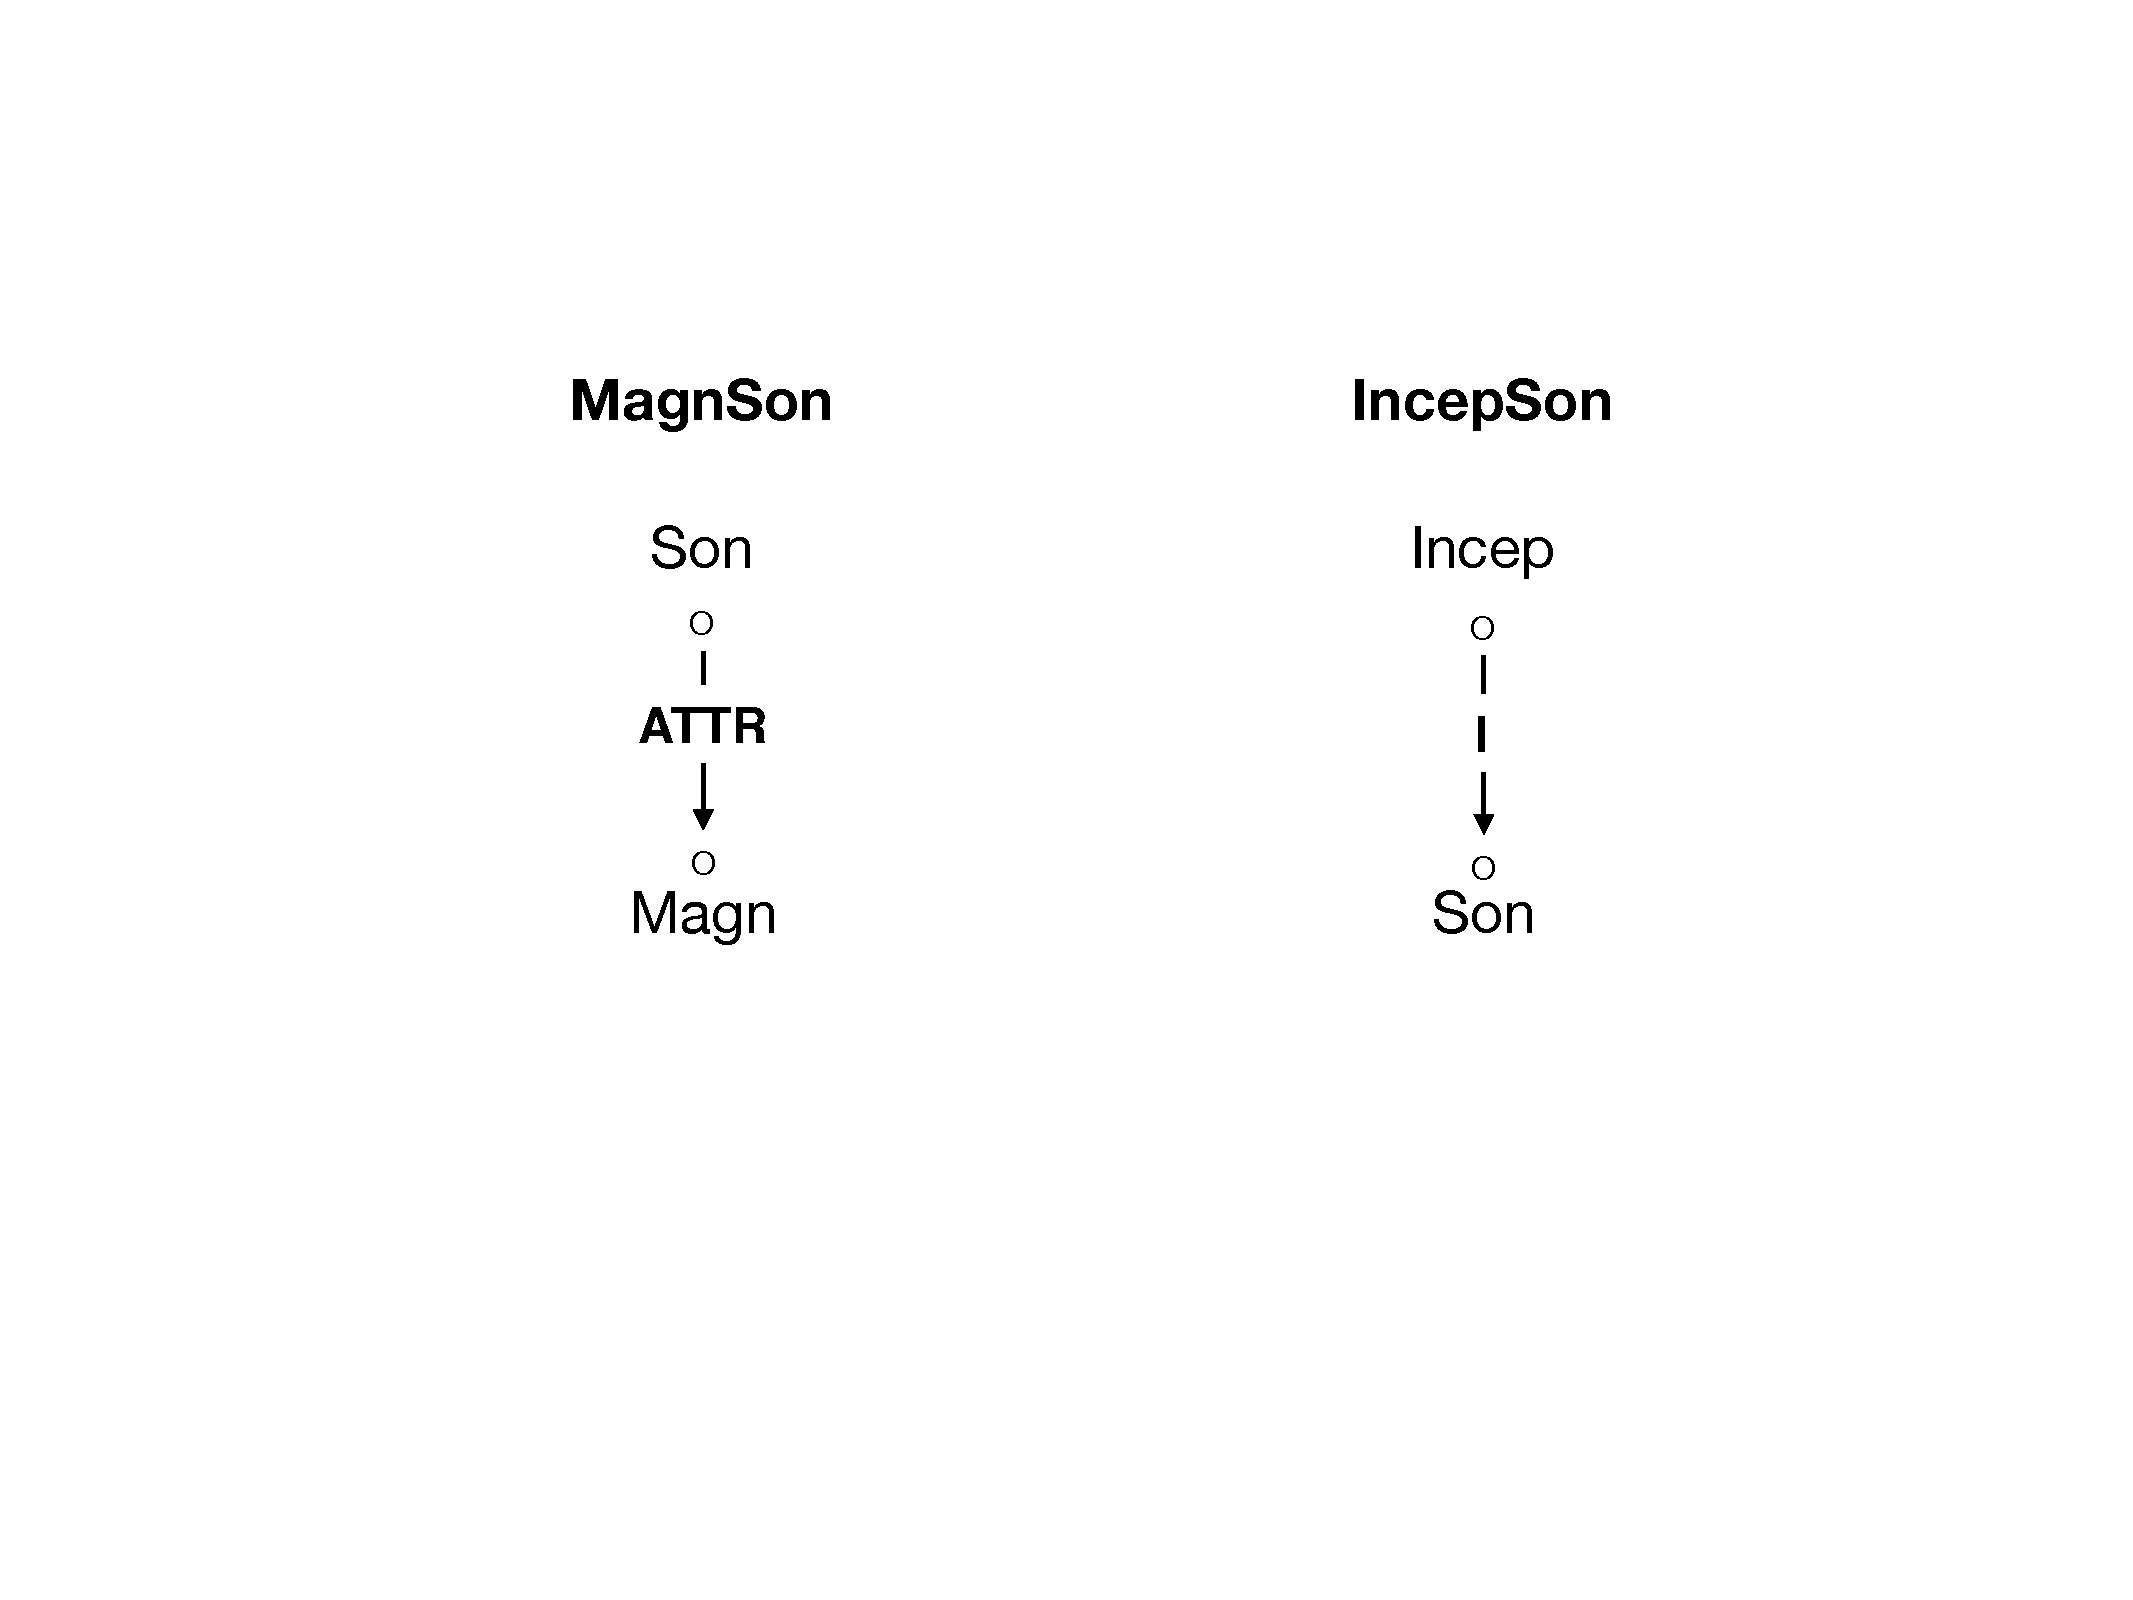
\includegraphics[width=5.3cm]{Fig/NotionLF/ComplexLFDSyntStruct.pdf}
\caption{DSyntSs of complex LFs \lf{MagnSon} and \lf{IncepSon}}\label{fig:ComplexLFDSyntStruct}
\end{figure}

\phantomsection\label{par:PoSComplexLF}\begin{soundbox}{Part of speech of a complex LF}
The head [=~top node] of the DSyntS of a complex LF gives its part of speech\index[notion]{complex LF!part of speech of a \tld}\index[notion]{lexical function!part of speech of a \tld}\index[notion]{part of speech [PoS]!\tld\ of an LF} to the value elements of this LF. For instance, the value of \lf{S\tsub{loc}Real\tsub{1}} -- whose DSyntS is \lf{S\tsub{loc}}\thinspace\syntRel{II}\thinspace\lf{Real\tsub{1}} -- is a noun (as \lf{S\tsub{loc}}), and the value of \lf{MagnSon} -- whose DSyntS is \lf{Magn}\thinspace\syntRelLeft{ATTR}\thinspace\lf{Son} -- is a verb (as \lf{Son}).

The part of speech of simple standard LFs is presented in detail in \sectref{sec:PofS} (p.\thinspace\pageref{sec:PofS}).

\end{soundbox}

A complex LF can consist of more than two simple LFs. For instance, \figref{fig:ComplexComplexLFDSyntStruct} shows the DSyntSs of such complex LFs exemplified in \Next:

\begingroup
\small

\ex. \a. \begingroup\setlength{\tabcolsep}{2pt}
\begin{tabular}[t]{ l l >{\raggedright\arraybackslash}p{7cm} }
\lfappl{AntiBonReal\tsub{1}}{\textit{chair}\tsub{(N)}} & = & \textit{slouch}\tsub{(V)}\textbf{,} \textit{slump}\tsub{(V)} \lfgp{\textit{in} \textsc{art} \tld} \\*
%\lfappl{A\tsub{1}AntiBonReal\tsub{1}}{\textit{chair}\tsub{(N)}} & = & \textit{slouched}\textbf{,} \textit{slumped} \lfgp{\textit{in} \textbf{\textsc{art}} \tld}\\
\end{tabular}\endgroup
    \b. \begingroup\setlength{\tabcolsep}{2pt}
\begin{tabular}[t]{ l l >{\raggedright\arraybackslash}p{6cm} }
\lfappl{CausPlusFact\tsub{0}}{\textit{screw}\tsub{(N)}} & = & \textit{tighten} \lfgp{\textsc{art}}\\[2pt]
\multicolumn{3}{>{\raggedright\arraybackslash}p{10cm}}{\remark{Note.}\lf{CausPlusFact\tsub{0}} is an abbreviation of \lf{CausPlusMagnFact\tsub{0}} -- see \chapref{chap:syntLFs}, [\ref{lf:Plus}], ``\nameref*{par:PlusMagn},'' p.\thinspace\pageref{par:PlusMagn}.} \\
\end{tabular}\endgroup

\endgroup

\begin{figure}

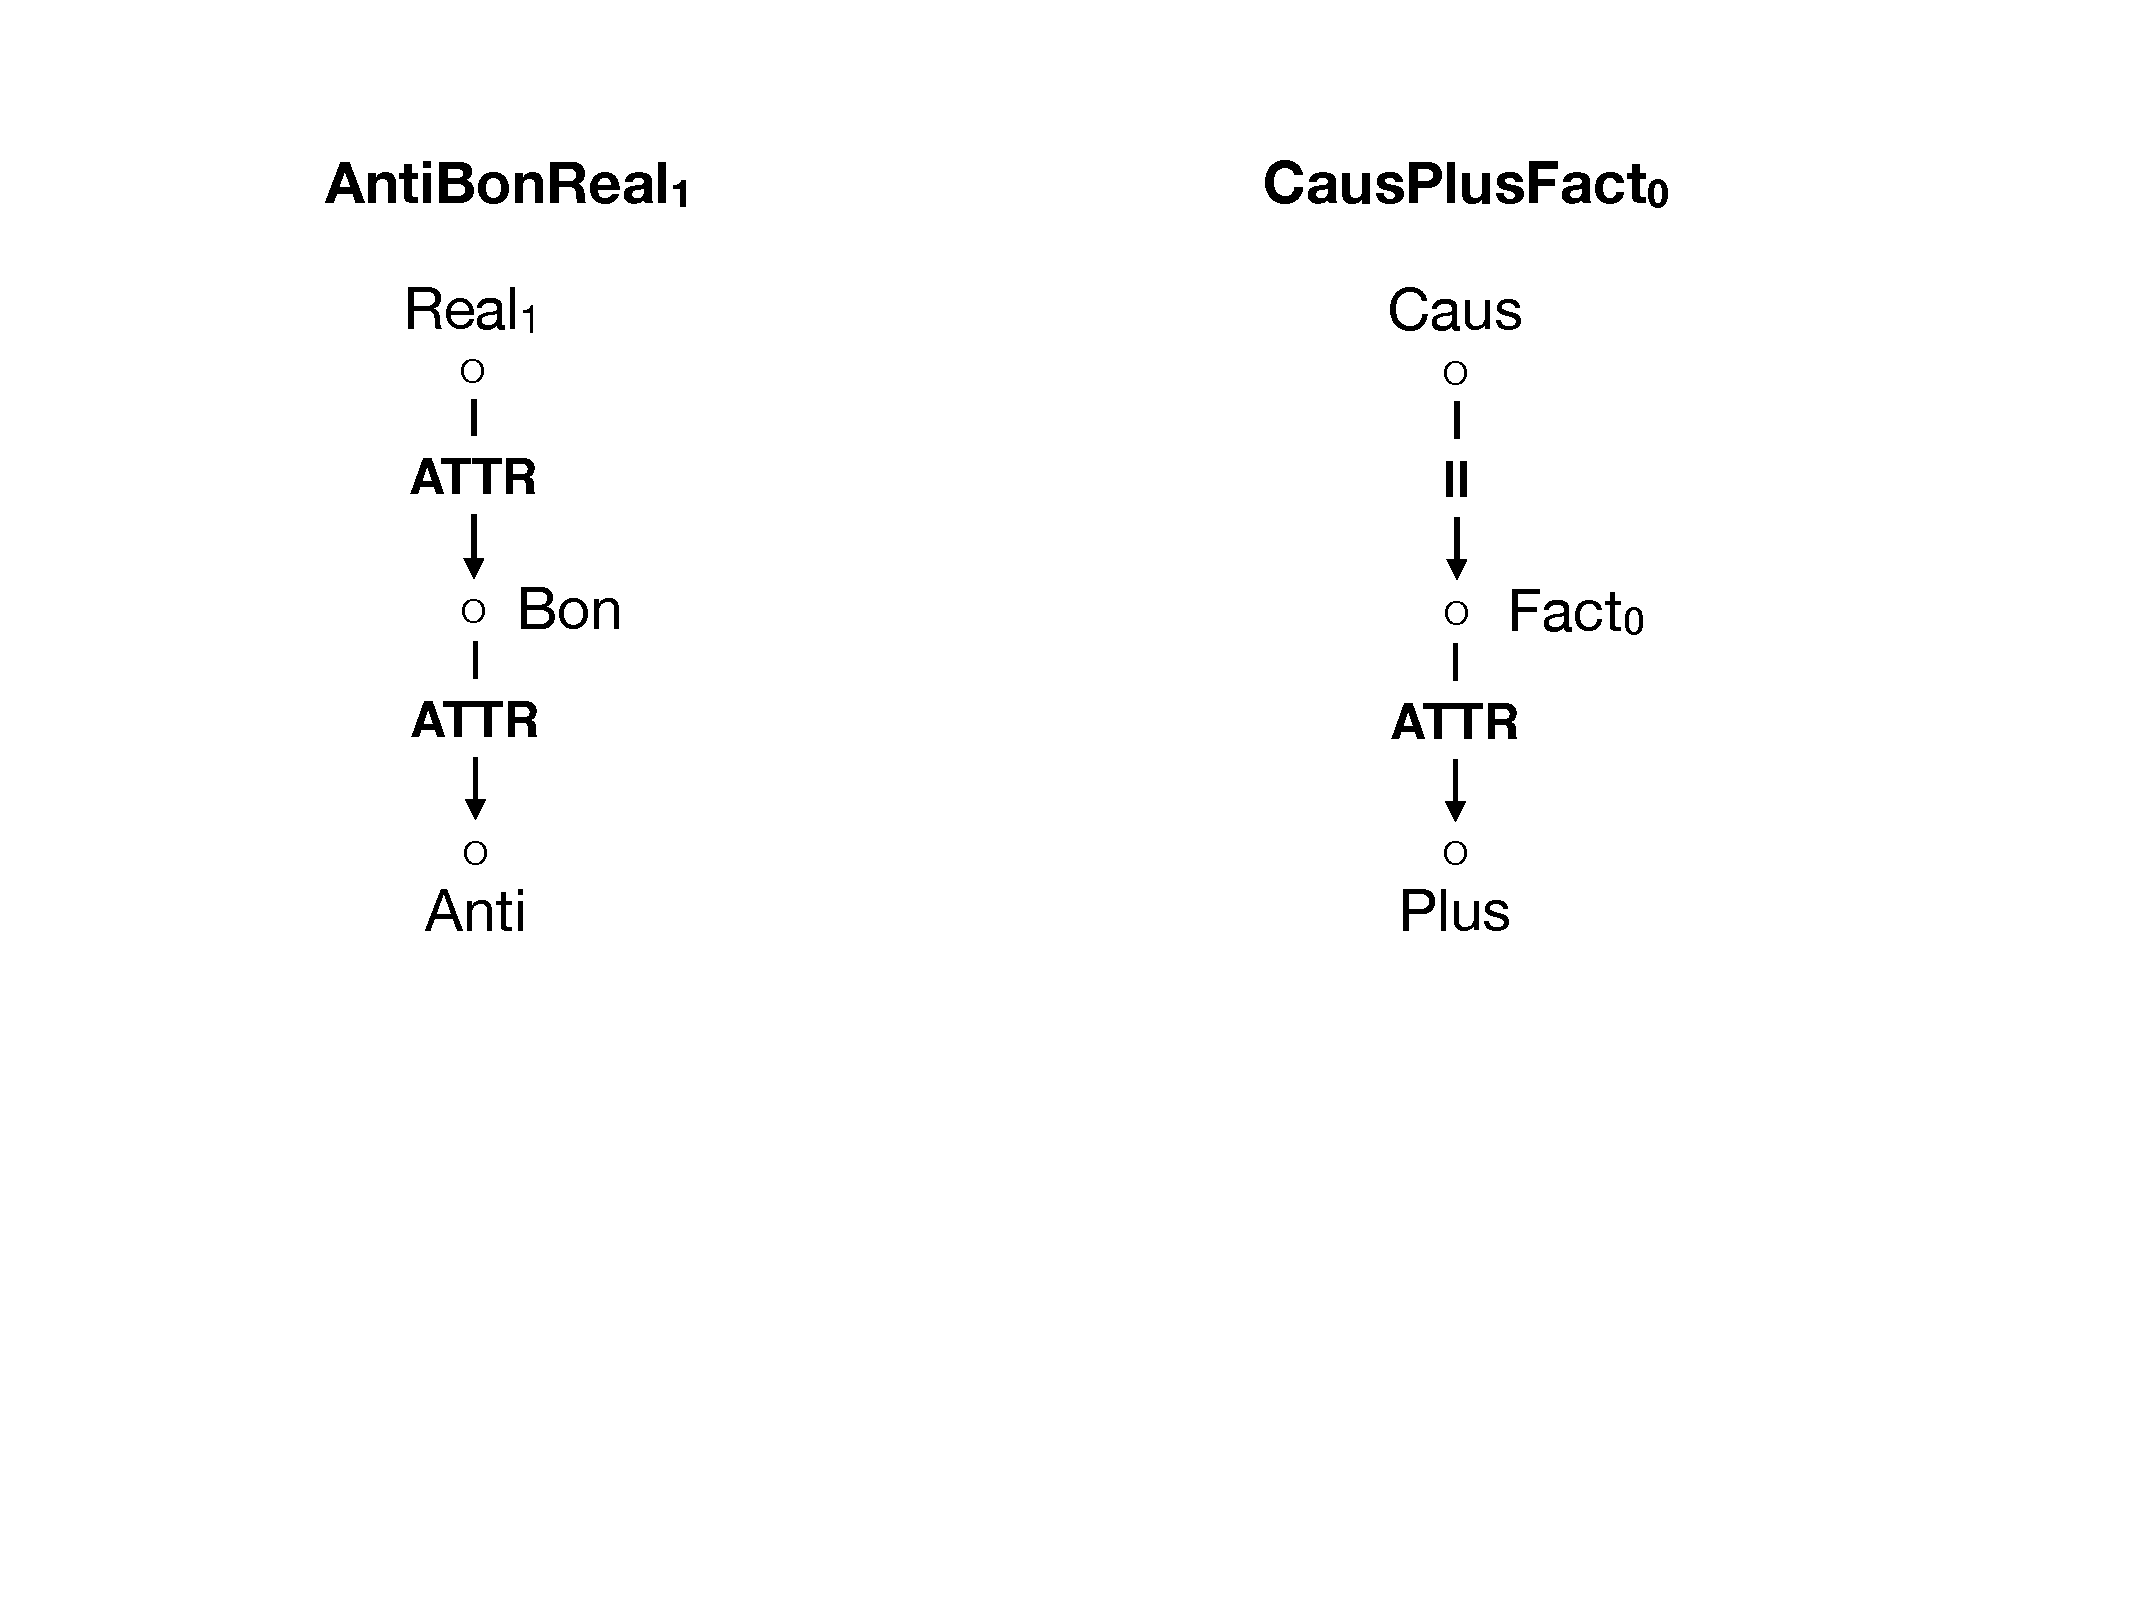
\includegraphics[width=6.7cm]{Fig/NotionLF/ComplexComplexLFDSyntStruct.pdf}
\caption{DSyntSs of complex LFs \lf{AntiBonReal\tsub{1}} and \lf{CausPlusFact\tsub{0}}}\label{fig:ComplexComplexLFDSyntStruct}
\end{figure}

\subsection{Configurational LFs}\label{sec:FLConfigurationnelles}\index[notion]{lexical function!configurational \tld|emph}\index[notion]{configurational LF|emph}

The combination of two LFs \lf{f\tsub{1}} and \lf{f\tsub{2}} can be such that both LFs apply to L simultaneously, but independently of each other and return a single value expressing jointly both LFs. This is represented by the following formula: \lfappl{f\tsub{1}+f\tsub{2}}{L}.

An \lf{f\tsub{1}+f\tsub{2}} configuration is called a \notion{configurational LF}. Compare the following pair of LFs:

\begingroup
\small

\ex. \begingroup\setlength{\tabcolsep}{2pt}
\begin{tabular}[t]{ l l >{\raggedright\arraybackslash}p{3cm} l }
\lfappl{A\tsub{1}}{\textit{sweat}\tsub{(V)}} & = & \textit{sweaty} & `who is sweating' \\*
\lfappl{Magn+A\tsub{1}}{\textit{sweat}\tsub{(V)}} & = & \textit{drenched in sweat}\tsub{(N)} & `who is sweating a lot'\vspace{3pt} \\
%\lfappl{A\tsub{1}}{\textit{despair}\tsub{(N)}} & = & \textit{in} \tld \\
%\lfappl{Magn\thinspace+\thinspace A\tsub{1}}{\textit{despair}\tsub{(N)}} & = & \idiom{\textit{in the pit}} \textit{of} \tld \\
\end{tabular}\endgroup

\endgroup\index[lf]{Magn@\lf{Magn}}\index[lf]{Ai@\lf{A\tsub{i}}!\lf{A\tsub{1}}}

\phantomsection\label{para:orderComponents}In a configurational LF \lf{f\tsub{1}+f\tsub{2}}, the order of components is relevant: \lf{f\tsub{2}} -- the rightmost LF -- is dominant, both syntactically and informationally. In the configuration \lf{f\tsub{1}+f\tsub{2}} where \lf{f\tsub{1}} and \lf{f\tsub{2}} are of different parts of speech\index[notion]{part of speech [PoS]!\tld\ of an LF}\index[notion]{lexical function!part of speech of a \tld}\index[notion]{configurational LF!part of speech of a \tld}, the component \lf{f\tsub{2}} imposes its part of speech on the value of the configurational LF, i.e., it dominates \lf{f\tsub{1}} syntactically. For instance, in the example below, the value is a verb, in accordance to the \lf{Oper\tsub{1}} component of the configurational LF:

\begingroup
\small

\ex. \begingroup\setlength{\tabcolsep}{2pt}
\begin{tabular}[t]{ l l >{\raggedright\arraybackslash}p{7cm} }
\lfappl{Magn+Oper\tsub{1}}{\textit{desire}\tsub{(N)}} & = & \textit{simmer} \lfgp{\textit{with} \tld} \\
\end{tabular}\endgroup

\endgroup\index[lf]{Magn@\lf{Magn}}\index[lf]{Operi@\lf{Oper\tsub{i}}!\lf{Oper\tsub{1}}}

If \lf{f\tsub{1}} and \lf{f\tsub{2}} are of the same part of speech -- e.g., both are modifying adjectives -- the meaning of \lf{f\tsub{2}} constitutes the informationally dominant component in the meaning of the value. For instance, the contrast between \lf{Bon+Magn} and \lf{Magn+Bon} is illustrated in \Next:

\begingroup
\small

\ex. \begingroup\setlength{\tabcolsep}{2pt}
\begin{tabular}[t]{ l l >{\raggedright\arraybackslash}p{2cm} l }
\lfappl{Bon+Magn}{\textit{meal}} & = & \textit{hearty} & `copious, and also good' \\*
\lfappl{Magn+Bon}{\textit{meal}} & = & \textit{somptuous} & `good, and also copious' \\
\end{tabular}\endgroup

\endgroup\index[lf]{Magn@\lf{Magn}}\index[lf]{Bon@\lf{Bon}}

\subsection{Actantial subscripts in LF combinations}\label{sec:actSubsLFCombinations}

\subsubsection{Actantial subscripts in complex LFs}

Two cases are to be distinguished for the actantial subscript to the name of a simple LF \lf{f\tsub{i}} used as a component of a complex LF (except for the rightmost one in the formula, which is interpretable in the standard way).

If \lf{f\tsub{i}} in a complex formula \lf{f\tsub{i}g} is not a verb of causing (\chapref{chap:syntLFs}, \sectref{sec:collocCausatif}\index[notion]{verb!\tld\ of causing}), its argument is the next simple LF \lf{g}, and  its actantial subscript ``\tsub{\lf{i}}'' refers to the DSyntA\thinspace\syntDname{i} of \lf{g}. For instance, in the complex LF \lf{A\tsub{1}Real\tsub{2}}\index[lf]{Ai@\lf{A\tsub{i}}!\lf{A\tsub{1}}}\index[lf]{Reali@\lf{Real\tsub{i}}!\lf{Real\tsub{2}}}, illustrated in \Next, ``\tsub{\lf{1}}'' refers to the DSyntA\thinspace\syntDname{I} of \lf{Real\tsub{2}} -- that is, to the sick person taking the medication.

\begingroup
\small

\ex. \lfappl{A\tsub{1}Real\tsub{2}}{\textit{medication} \lfgp{\textit{prescribed by X to Y against Z}}} = \textit{medicated}\textbf{,} \textit{on} \tld

\endgroup

The actantial subscripts of the LF \lf{A\tsub{1}Real\tsub{2}} used in \Last are interpretable as follows:

\begin{itemize}

\item The lexical unit \textsc{medication} controls three DSyntAs: DSyntA\thinspace\sensenum{I} is the doctor X; DSyntA\thinspace\sensenum{II}, the sick person Y; DSyntA\thinspace\sensenum{III}, the illness Z.

\item \lfappl{Real\tsub{2}}{\textit{medication}} -- \lfgp{\textit{Y}} \textit{takes} \lfgp{\textit{a medication}} -- controls, by definition of the LF \lf{Real\tsub{i}} (\chapref{chap:syntLFs}, [\ref{lf:Real-i}], p.\thinspace\pageref{lf:Real-i}), two DSyntAs:

\begin{itemize}

\item DSyntA\thinspace\syntDname{I}, the sick person Y -- cf. ``\tsub{\lf{2}}'' in \lf{Real\tsub{\textbf{2}}} (since Y is DSyntA~\syntDname{II} of \textsc{medication});
 
 \item DSyntA\thinspace\syntDname{II}, the noun \textsc{medication}.

\end{itemize}

\item The subscript ``\tsub{\lf{1}}'' of \lf{A\tsub{1}} in the formula \lf{A\tsub{1}Real\tsub{2}} refers to the DSyntA\thinspace\syntDname{I} of its argument \lf{Real\tsub{2}}, that is, to the sick person Y (and not to the DSyntA\thinspace\sensenum{I} of \textsc{medication}, that is, to the doctor~X).

\end{itemize}

If \lf{f\tsub{i}} is  a verb of causing, its actantial subscript\index[notion]{actantial subscript!\tld\ of a verb of causing LF} ``\tsub{i}'' refers to the corresponding DSyntA of L, just as it does when this LF is used alone. For instance, in the complex LF \lf{Caus\tsub{2}Oper\tsub{2}}\index[lf]{Caus@\lf{Caus}!\lf{Caus\tsub{2}}}\index[lf]{Operi@\lf{Oper\tsub{i}}!\lf{Oper\tsub{2}}} illustrated in \Next, the subscript ``\tsub{\lf{2}}'' of \lf{Caus\tsub{2}} refers to the DSyntA\thinspace\syntDname{II} of \textit{trust}\tsub{(N)}, that is, to the person who is trusted:

\begingroup
\small

\ex. \lfappl{Caus\tsub{2}Oper\tsub{2}}{\textit{trust}\tsub{(N)} \lfgp{\textit{of X in Y}}} = \textit{win}\tsub{(V)} \lfgp{\textsc{art} \tld} \\
     Ex.: \textit{Joey}\tsub{Y} \textit{won}\tsub{\lfappl{Caus$_\text{2}$Oper$_\text{2}$}{\textit{trust}\tsub{(N)}}} \textit{the trust of Chandler}\tsub{X}\textit{.}

\endgroup

\subsubsection{Actantial subscripts in configurational LFs}

There is nothing  particular to be said about actantial subscripts\index[notion]{actantial subscript} in configurational LFs: the components of these LFs are either simple LFs, or complex LFs, and the explanations about actantial subscripts in these two types of LFs have already been provided.

\section{Parts of speech of simple standard LFs}\label{sec:PofS}

Since an LF is a deep lexical unit\index[notion]{lexical unit!deep \tld} (cf.~\ref{sec:LFAsDeepLU}, p.\thinspace\pageref{sec:LFAsDeepLU}), it belongs to a part of speech\index[notion]{lexical function!part of speech of a \tld}\index[notion]{part of speech [PoS]!\tld\ of an LF}. More specifically, as we will see, it has only a deep-syntactic part of speech.

\subsection{Notion of part of speech [PoS]}\label{sec:notionPdD}

A \notion{part of speech}\index[notion]{part of speech [PoS]|emph} [\notion{PoS}\index[notion]{PoS|see{part of speech}}] is a major class of lexical units that feature, at the syntactic level, the same \notion{passive syntactic valence}\index[notion]{valence!passive syntactic \tld|emph}. By passive syntactic valence of a lexical unit, we mean its ability to participate in particular syntactic constructions as the dependent\index[notion]{dependent, syntactic} member \parencite[109]{Melcuk2015a-e}:\footnote{Passive syntactic valence is to be contrasted with active syntactic valence, introduced in \chapref{chap:preliminaryNotions}, \sectref{sec:syntacticNotions}, p.\thinspace\pageref{para:activeSyntacticValence}.}\index[notion]{valence!active syntactic \tld}

\begin{itemize}

\item a verb -- in a finite form -- is typically the syntactic head of a clause and need not be dependent;
\item a noun is typically a syntactic actant;
\item an adjective is typically a modifier of a noun;
\item etc.

\end{itemize}

Two types of PoS are distinguished: deep PoS and surface PoS. There are five \notion{deep parts of speech}\index[notion]{part of speech [PoS]!deep \tld|emph}:

\begin{itemize}

\item \notion{Verb} [\notion{V}]\index[notion]{verb!Verb [V]|emph}\index[notion]{part of speech [PoS]!V(erb)|emph},
\item \notion{Noun} [\notion{N}]\index[notion]{noun!Noun [N]|emph}\index[notion]{part of speech [PoS]!N(oun)|emph},
\item \notion{Adjective} [\notion{Adj}]\index[notion]{adjective!Adjective [Adj]|emph}\index[notion]{part of speech [PoS]!Adj(ective)|emph},
\item \notion{Adverb} [\notion{Adv}]\index[notion]{adverb!Adverb [Adv]|emph}\index[notion]{part of speech [PoS]!Adv(erb)|emph},
\item \notion{Clausative} [\notion{Claus}]\index[notion]{clausative!Clausative [Claus]|emph}\index[notion]{part of speech [PoS]!Claus(ative)|emph}.

\end{itemize}

V, N, Adj and Adv do not call for further remarks. Claus, on the other hand, needs an explanation: a clausative is a lexical expression that is syntactically equivalent to an independent clause and is not a verb.\footnote{\textcite[Ch.~45]{Tesniere1959} calls such expressions \textit{mots phrases} or \textit{phrasillons}.} \phantomsection\label{txt:Claus0}Clausatives form a very heterogenous lexical class, which includes emotional interjections\index[notion]{interjection} (\textsc{Wow!}, \textsc{Yuck!}) and onomatopoeic interjections\index[notion]{onomatopoeia}\index[notion]{interjection!onomatopoeic \tld} (\textsc{Meow!}, \textsc{Bang!}), as well as interjection-like lexemes (\textsc{Well}) and fixed phrases (\idiom{\textsc{Bless you}} \lfgp{to someone who just sneezed}\footnote{Even if \textsc{bless} is inherently a verb, the phrase \textit{Bless you!} is not a verbal phrase: the form \textit{bless} in it obviously cannot be considered an imperative, and neither can it be taken to be a finite form, since it has no subject. This form is ``frozen'' not only semantically, but also syntactically.}).

Deep PoS are linguistically universal\index[notion]{language-universal} in the sense that they are necessary and sufficient for describing deep-syntactic structures\index[notion]{structure!deep-syntactic \tld\ [DSyntS]}\index[notion]{deep-syntactic!\tld\ structure [DSyntS]} of sentences in any language.

In contrast to deep PoS, \notion{surface PoS}\index[notion]{part of speech [PoS]!surface \tld|emph} are not linguistically universal: each language features its own set of surface PoS. Thus, English has prepositions\index[notion]{preposition}, while Hungarian has only postpositions\index[notion]{postposition}; English has determiners\index[notion]{determiner}, while Russian does not. A given surface PoS is a ``particular case'' of a deep PoS: prepositions and conjunctions\index[notion]{conjunction} are subtypes of deep adverbs (Adv)\index[notion]{adverb};\footnote{More precisely, prepositions and conjunctions form a subclass of adverbs that have an obligatory DSyntA\thinspace\syntDname{II} (on DSyntA, see \chapref{chap:preliminaryNotions}, \sectref{sec:syntacticNotions}, p.\thinspace\pageref{def:DSyntA}).}\index[notion]{actant!deep-syntactic \tld\ [DSyntA]}\index[notion]{deep-syntactic!\tld\ actant [DSyntA]} determiners are subtypes of deep adjectives\index[notion]{adjective} (Adj); etc. On deep vs. surface PoS, see \textcite[Ch.~7, Sec.~2.1.3, 49--51]{Melcuk2013c-e}.\phantomsection\label{txt:PrepAdv}

In what follows, only deep PoS are considered, so that the adjective \textit{deep} can be omitted.

To conclude, note that the PoS of a lexical unit L is a core element of L's cooccurrence\index[notion]{cooccurrence, restricted}; as such, it can be expected to be the first piece of information given in L's lexical entry\index[notion]{lexical entry}\index[notion]{lexicography} -- see e.g., the lexical entry of \textsc{anger}\tsub{(N)} in the Appendix (p.\thinspace\pageref{chap:appendix1}).

\subsection{LF's inherent PoS}\label{sec:LFsInherentPoS}

Most simple standard LFs possess an inherent PoS\index[notion]{part of speech [PoS]!\tld\ of an LF}\index[notion]{lexical function!part of speech of a \tld}: e.g., \lfappl{S\tsub{i}}{L}\index[lf]{Si@\lf{S\tsub{i}}} is always a noun, and \lfappl{Oper\tsub{i}}{L}\index[lf]{Operi@\lf{Oper\tsub{i}}} is always a verb. However, several paradigmatic LFs borrow their PoS from their argument. Such LFs are:

\begin{itemize}

\item the three ``meta''-LFs, which underlie the whole LF system\index[notion]{lexical function!system of standard \tlds}\index[notion]{system of standard LFs}: \lf{Syn}\index[lf]{Syn@\lf{Syn}}, \lf{Conv\tsub{ijk}}\index[lf]{Convijk@\lf{Conv\tsub{ijk}}} and \lf{Anti}\index[lf]{Anti@\lf{Anti}} (with \lf{Contr}\index[lf]{Contr@\lf{Contr}}) -- \chapref{chap:paraLFs}, \sectref{sec:troisPiliersFL}, p.\thinspace\pageref{sec:troisPiliersFL};

\item the ``semantic pronoun'': \lf{Gener}\index[lf]{Gener@\lf{Gener}} -- \chapref{chap:paraLFs}, [\ref{lf:Gener}], p.\thinspace\pageref{lf:Gener};

\item two LFs whose meanings are close to those of grammemes\index[notion]{grammeme}: the singulative \lf{Sing}\index[lf]{Sing@\lf{Sing}} and the collective \lf{Mult}\index[lf]{Mult@\lf{Mult}} -- \chapref{chap:paraLFs}, \sectref{sec:flFlexion}, p.\thinspace\pageref{sec:flFlexion}.

\end{itemize}

For the PoS of complex LFs\index[notion]{lexical function!complex \tld}\index[notion]{complex LF}, see \sectref{sec:FLComplexes}, p.\thinspace\pageref{par:PoSComplexLF}.

\paragraph*{Part of speech tables for LF applications.}\label{par:LFPoSTable}\index[notion]{application of an LF!part of speech of the \tld}

An LF \lf{f} calls for two syntactic characteristics as regards PoS: (i)~the PoS of its possible arguments L and (ii)~the corresponding PoS of its value -- a deep lexical unit\index[notion]{lexical unit!deep \tld} \lfappl{f}{L}.

This correspondence is shown in a \notion{PoS table}\index[notion]{part of speech [PoS]!\tld\ table|emph} for each LF. Take as example the PoS table of \lf{Magn}\index[lf]{Magn@\lf{Magn}}, intensification modifier:

\begin{quote}
\small
\begin{tabular}{ l c c c c c }
   \midrule
   \multicolumn{6}{l}{\lf{Magn}: adjectival\slashs{}adverbial} \\
   \midrule
   \textbf{L} & V & N & Adj & Adv & Claus \\
%   \midrule
   \textbf{\lfappl{Magn}{L}} & Adv & Adj & Adv & Adv & Adj\slashs{}Adv \\
   \midrule
\end{tabular}
\end{quote}

The table header indicates that \lf{Magn} is a modifier that functions as an adjective\index[notion]{adjective} or an adverb\index[notion]{adverb}. The body of the table specifies the correspondence between the PoS of L and that of the deep lexical unit \lfappl{Magn}{L} -- i.e., the PoS of \lf{Magn} itself, for short.

When a PoS correspondence is theoretically possible, but not attested to our knowledge, the symbol ``\lfgp{?}'' is added. The PoS table of \lf{Gener}\index[lf]{Gener@\lf{Gener}} illustrates this situation.

\begin{quote}
\small
\begin{tabular}{ l c c c c c }
   \midrule
   \multicolumn{6}{l}{\lf{Gener}: borrows L's PoS} \\
   \midrule
   \textbf{L} & V & N & Adj & Adv & Claus \\
   \midrule
   \textbf{\lfappl{Gener}{L}} & V & N & Adj & Adv & Claus\lfgp{?} \\
   \midrule
\end{tabular}
\end{quote} 

In the header of this table, the statement ``borrows L's PoS'' indicates that \lf{Gener} is an LF without inherent PoS\index[notion]{part of speech [PoS]!inherent \tld}.

\section{Regularities in standard LFs}\label{sec:regularitiesInLFs}

In spite of the basically idiosyncratic character of LFs, in many cases a given LF has the same values for quite a few different arguments: you \textit{take a bath}, \textit{a shower}, \textit{a rest}, ...; you \textit{are in despair}, \textit{love}, \textit{a rage}, ...; you \textit{follow the rules}, \textit{prescriptions}, \textit{recommendations}, \textit{instructions}, ... The reason is, of course, semantic proximity of these LF's arguments: semantically related lexical units tend to feature the same values for a given LF.

In other words, there exist \notion{regularities}\index[notion]{regularity|emph} among LFs of any natural language. No doubt that such regularities play an important role in the acquisition of LFs by speakers, as the former allow the latter to make predictions about LFs. These regularities should be exploited in such domains as language teaching\index[notion]{teaching\slashs{}learning, language}\index[notion]{language teaching\slashs{}learning}, translation, etc. It is therefore important to extract them, and formulate \notion{generalizations}\index[notion]{generalization concerning LFs|emph}, which should be stored in models of the lexicon\index[notion]{lexicon!\tld\ model}\index[notion]{model!lexicon \tld} in a way that supports the \notion{inheritance}\index[notion]{inheritance!\tld\ of regularities}\index[notion]{regularity!inheritance of \tld{ies}} of regularities \parencite{MelcukWanner1996}.

The elements of the values of an LF \lf{f} shared by several argument lexical units can be generalized by extracting them from individual lexical entries\index[notion]{lexical entry} of these units and storing them together: either on the argument side (for a group of lexical units) or on the LF side (attaching them to the LF itself). In practice, both methods can be  combined in different proportions. We propose below four types of generalizations, that is, we indicate types of regularities with associated means of accounting for them: generalizations at vocable's level (\sectref{sec:generalizationVocable}), generalizations associated with a generic term (\sectref{sec:generalizationsGener}), joker values\index[notion]{value of an LF!joker \tld}\index[notion]{joker value of an LF}\index[notion]{lexical function!joker value of a \tld} associated with given LFs (\sectref{sec:jokerValuesAssociatedGivenLFs}) and lexical entries for collocative lexical units (\sectref{sec:lexicalEntriesCollocativesLUs}).

\subsection{Generalizations at vocable's level}\label{sec:generalizationVocable}\index[notion]{generalization concerning LFs!\tld\ associated with a vocable}\index[notion]{vocable}

If several lexical units of a given vocable or of several semantically-related vocables share LF values, these values can be given under one of these units, with a cross-reference in the lexical entries\index[notion]{lexical entry} of the others. For instance, we have for the verb \textsc{escape}{\tsub{(V)}}:

\begingroup
\small

\ex. \begingroup\setlength{\tabcolsep}{2pt}
\begin{tabular}[t]{ l l >{\raggedright\arraybackslash}p{7cm} }
\lf{S\tsub{1}} & : & \textit{escaper} \\
\lf{S\tsub{1}Perf} & : & \textit{escapee}\textbf{,} \textit{fugitive}\tsub{(N)}\textbf{,} \textit{runaway}\tsub{(N)} \\
\lf{S\tsub{1}Able\tsub{1}} & : & \idiom{\textit{flight risk}} \\
%\lf{S$_\text{1}^\text{usual}$} & : & ... \\
\lf{S\tsub{2}} & : & \idiom{\textit{place of detention}} \\
\lf{A\tsub{1}} & : & \textit{fugitive}\tsub{(Adj)}\textbf{,} \textit{runaway}\tsub{(Adj)} \\*
\lf{Able\tsub{2}} & : & \textit{escapable} \\
\end{tabular}\endgroup

\endgroup\index[lf]{Si@\lf{S\tsub{i}}!\lf{S\tsub{1}}}\index[lf]{Perf@\lf{Perf}}\index[lf]{Ablei@\lf{Able\tsub{i}}!\lf{Able\tsub{1}}}\index[lf]{Ablei@\lf{Able\tsub{i}}!\lf{Able\tsub{2}}}\index[lf]{Si@\lf{S\tsub{i}}!\lf{S\tsub{2}}}\index[lf]{Ai@\lf{A\tsub{i}}!\lf{A\tsub{1}}}

As the same LF relations hold for the corresponding noun \textsc{escape}\tsub{(N)}, which is the \lf{S\tsub{0}}\index[lf]{S0@\lf{S\tsub{0}}} (nominalization) of the verb, we can simply indicate the following cross-reference in its lexical entry\index[notion]{lexical entry}:

\begingroup
\small

\ex. \begingroup\setlength{\tabcolsep}{2pt}
\begin{tabular}[t]{ l l >{\raggedright\arraybackslash}p{6cm} }
\lf{S\tsub{1}}\textbf{,} \lf{S\tsub{1}Perf}\textbf{,} \lf{S\tsub{1}Able\tsub{1}}\textbf{,} \lf{S\tsub{2}}\textbf{,} \lf{A\tsub{1}}\textbf{,} \lf{Able\tsub{2}} & : & $\pmb{\uparrow}$\thinspace\textsc{escape}\tsub{(V)} \\
\end{tabular}\endgroup

\endgroup

Note that \Last, which concerns two specific lexical units (\textsc{escape}\tsub{(V)} and \textsc{escape}\tsub{(N)}), is in point of fact a consequence of a series of more general statements concerning the entire system of LFs itself, namely:

\begingroup
\small

\ex. \begingroup\setlength{\tabcolsep}{2pt}
\begin{tabular}[t]{ l c >{\raggedright\arraybackslash}p{7cm} }
\lfappl{S\tsub{i}}{L\tsub{(V)}} & = & \lfappl{S\tsub{i}}{\lfappl{S\tsub{0}}{L\tsub{(V)}}} \\*
... & & \\
\lfappl{A\tsub{i}}{L\tsub{(V)}} & = & \lfappl{A\tsub{i}}{\lfappl{S\tsub{0}}{L\tsub{(V)}}} \\*
... & & \\
\end{tabular}\endgroup

\endgroup

\subsection{Generalizations associated with a generic term}\label{sec:generalizationsGener}\index[notion]{generalization concerning LFs!\tld\ associated with a generic term}

There are semantic classes\index[notion]{semantic!\tld\ class} of lexical units such that:

\begin{enumerate}

\item they all belong to the same semantic field\index[notion]{semantic!\tld\ field};

\item they possess the same generic term\index[notion]{generic term}\index[lf]{Gener@\lf{Gener}} L\tsub{\textsc{gener}}\footnote{On generic terms, see the LF \lf{Gener}, \chapref{chap:paraLFs}, [\ref{lf:Gener}], p.\thinspace\pageref{lf:Gener}.} -- for instance, \textsc{car}, \textsc{truck}\tsub{(N)}, \textsc{van}, \textsc{bus}\tsub{(N)}, \textsc{motorbike}\tsub{(N)}, ... form a semantic class united under the same L\tsub{\textsc{gener}} \textsc{vehicle} in the sense of `motor vehicle';

\item the meaning of L\tsub{\textsc{gener}} is sufficiently rich so that it belongs to the same semantic field as these lexical units -- cf., \textsc{vehicle} belongs to the same semantic field as \textsc{car}, \textsc{truck}\tsub{(N)}, etc.

\end{enumerate}

Elements of such semantic classes may share the same values for some LFs. (This is only a tendency, with many exceptions, yet in some cases this tendency is quite clear.) If such is the case, generalizations can be made by storing all common values of LFs supplied with necessary constraints under a special \notion{public zone}\index[notion]{lexical entry!public zone of a \tld|emph}\index[notion]{zone of a lexical entry!public \tld|emph} of L\tsub{\textsc{gener}}'s lexical entry. For instance, if the following is stored in the public zone of the lexical entry for \textsc{vehicle}, it does not need to be repeated in the lexical entry for all names of vehicles:

\begin{center}
\footnotesize
\APolbox{10.8cm}{%
\renewcommand*{\arraystretch}{1}
\setlength{\tabcolsep}{2.5pt}
\begin{tabular}{ l l l }
\multicolumn{3}{l}{\textsc{vehicle}, noun} \\
... & & \\
\multicolumn{3}{l}{\textbf{\textsf{Public}}} \vspace{-3pt}\\
... & & \\
\lf{S\tsub{1}}\index[lf]{Si@\lf{S\tsub{i}}!\lf{S\tsub{1}}} & : & \textit{driver}\textbf{;} \textit{rider} \lfconstr{for two-wheel vehicle} \\
\lf{S\tsub{2}}\index[lf]{Si@\lf{S\tsub{i}}!\lf{S\tsub{2}}} & : & \textit{passenger} \\
... & & \\
\lf{Real\tsub{1}}\index[lf]{Reali@\lf{Real\tsub{i}}!\lf{Real\tsub{1}}} \lfgp{i.e., `use \tld\ as driver'} & : & \textit{drive}\tsub{(V)} \lfgp{\textsc{art} \tld}\textbf{;} \textit{ride}\tsub{(V)}\sensenumonly{1} \lfgp{\textsc{art} \tld} \lfconstr{for two-wheel vehicle} \\
\lf{Real\tsub{2}}\index[lf]{Reali@\lf{Real\tsub{i}}!\lf{Real\tsub{2}}} \lfgp{i.e., `use \tld\ as passenger'} & : & \textit{ride}\tsub{(V)}\sensenumonly{2} \lfgp{(\textit{in}\slashs\textit{on}) \textsc{art} \tld}\textbf{,} \textit{go} \lfgp{\textit{by} \tld} \\
... & & \\
\end{tabular}
}
\end{center}

A rather straightforward particular case of the above type generalization is the use of LFs with proper names\index[notion]{proper name}\index[notion]{noun!proper name \tld}. If the argument of an LF \lf{f} happens to be a proper name N\tsub{(prop)}, the value of \lf{f} must be computed substituting for N\tsub{(prop)} the lexical unit L that denotes the entity named by N\tsub{(prop)}. In other words, the values of LFs for \textsc{Rhine}, \textsc{Ganges}, \textsc{Volga}, \textsc{Thames}, \textsc{Mississippi}, etc. are those of the LFs for \textsc{river} (or \textsc{watercourse}):

\begingroup
\small

\ex. \a. The Rhine $\langle$This river$\rangle$ \emph{flows} from Switzerland to the North Sea.
     \b. The Ganges $\langle$This river$\rangle$ \emph{empties} into the Bay of Bengal.
     \c. The Oka $\langle$This river$\rangle$ is a \emph{tributary} of the Volga.
     \d. The Thames $\langle$This river$\rangle$ was \emph{swollen} and \emph{flooding} the riverbanks.

\endgroup

\subsection{Joker values associated with given LFs}\label{sec:jokerValuesAssociatedGivenLFs}\index[notion]{generalization concerning LFs!\tld\ associated with an LF}\index[notion]{value of an LF!joker \tld|emph}\index[notion]{joker value of an LF|emph}\index[notion]{lexical function!joker value of a \tld|emph}

The level of generality of LF values might be such that it becomes feasible to associate with a given LF some general default elements of its value: we refer to such default elements as \notion{joker values}. Thus, a generally valid expression in English of the LF \lf{S\tsub{0}}\index[lf]{S0@\lf{S\tsub{0}}!joker \tld} for a verb L\tsub{(V)} is the phrase \textit{the fact of V-ing} -- or just simply \textit{V-ing}; e.g.:

\begingroup
\small

\ex. \begin{tabular}[t]{ l l l }
\lfappl{joker S\tsub{0}}{\textit{chew}\tsub{(V)}} & = & \textit{the fact of chewing}\textbf{,} \textit{the chewing} \\
\lfappl{joker S\tsub{0}}{\textit{ponder}} & = & \textit{the fact of pondering}\textbf{,} \textit{the pondering} \\
\end{tabular}

\endgroup

For the support verbs\index[notion]{support verb}\index[notion]{verb!support \tld} \lfappl{Oper\tsub{1}}{L}\index[lf]{Operi@\lf{Oper\tsub{i}}!joker \lf{Oper\tsub{1}}}, the joker value elements are \textsc{do}, \textsc{make}, \textsc{give}, \textsc{have}, \textsc{take}, \idiom{\textsc{carry out}} and maybe some more. Of course, for each of those, semantic restrictions on L have to be specified. For \lfappl{Func\tsub{0}}{L}\index[lf]{Funci@\lf{Func\tsub{i}}!joker \lf{Func\tsub{0}}} -- another type of support verbs, joker value elements are, among others, \idiom{\textsc{take place}}, \textsc{happen} (for L denoting a social event), etc. For intensifiers \lfappl{Magn}{L}\index[lf]{Magn@\lf{Magn}!joker \tld}, when they have nominal arguments, such general elements are: \textsc{big}\tsub{(Adj)}, \textsc{high}\tsub{(Adj)} (for L denoting non-linear physical parameters such as \textsc{pressure}\tsub{(N)}, \textsc{speed}\tsub{(N)}, \textsc{temperature}), \textsc{utmost}\tsub{(Adj)}\slashs\textsc{utter}\tsub{(Adj)} (for feelings), etc. An obvious \lf{Magn} joker value element for adjectival lexemes as arguments is \textsc{very}.

The generalizations considered here are directly associated with LFs and their description presupposes the existence of special lexical entries dedicated to LFs\index[notion]{lexical entry!\tld\ for an LF}.

\subsection{Lexical entries for collocative lexical units}\label{sec:lexicalEntriesCollocativesLUs}\index[notion]{lexical entry}\index[notion]{generalization concerning LFs!\tld\ associated with a collocative lexical unit}

\notion{Collocative lexical units}\index[notion]{lexical unit!collocative \tld|emph} are ``designed'' to be selected by the Speaker as values of syntagmatic LFs\index[notion]{lexical function!syntagmatic \tld}\index[notion]{syntagmatic!\tld\ lexical function}: they have virtually no autonomy and are essentially used as collocates\index[notion]{collocation!collocate of a \tld} within collocations\index[notion]{collocation}.

To ensure a sufficiently systematic description of collocative lexical units shared by many collocation bases\index[notion]{base!\tld\ of a collocation}\index[notion]{collocation!base of a \tld}, one has to compile for them special lexical entries\index[notion]{lexical entry!\tld\ for a collocative lexical unit}, where semantic and syntactic conditions on their use are specified. Thus, the support verb\index[notion]{support verb}\index[notion]{verb!support \tld} \textit{deliver} is an element of the value of the LF \lf{Oper\tsub{1}}\index[lf]{Operi@\lf{Oper\tsub{i}}!\lf{Oper\tsub{1}}} for many nouns of public activities (\textit{deliver a speech}\slashs\textit{a lecture}\slashs\textit{a performance}). It receives a lexical entry of its own in the vocable\index[notion]{vocable} \textsc{deliver}; accordingly, it need not be lexicographically described in all lexical entries for nouns it combines with but can be selected and used following indications found in its own entry.

For an example of a dictionary of collocations\index[notion]{dictionary!\tld\ of collocations}\index[notion]{collocation!dictionary of \tlds} with entries for collocates, see \textcite{Bosque2010}.

To round up the topic, still another perspective of possible generalizations for LFs is opened by accounting for the links between the meaning of a lexical unit L and the LFs applicable to it; for instance:

\begin{itemize}

\item L that is predicative\index[notion]{predicativity} expects actantial paradigmatic derivatives\index[notion]{derivative!semantic \tld}\index[notion]{semantic!\tld\ derivative} -- cf. LFs \lf{S\tsub{i}}\index[lf]{Si@\lf{S\tsub{i}}}, \lf{A\tsub{i}}\index[lf]{Ai@\lf{A\tsub{i}}}, ..., and syntagmatic verbal collocates such as support verbs\index[notion]{support verb}\index[notion]{verb!support \tld} (\lf{Oper\tsub{i}}\index[lf]{Operi@\lf{Oper\tsub{i}}}, ...) and possibly realization verbs\index[notion]{verb!realization \tld}\index[notion]{realization verb} (\lf{Real\tsub{i}}\index[lf]{Reali@\lf{Real\tsub{i}}}, ...).

\item L that denotes an artefact expects realization verbs such as \lf{Real\tsub{1}}\index[lf]{Rea|li@\lf{Real\tsub{i}}!\lf{Real\tsub{1}}}, which expresses `make use of L'.

\item L that denotes something producing sounds expects values for the LF \lf{Son}\index[lf]{Son@\lf{Son}}.

\item L that denotes an inner state of a human expects values for the LFs \lf{Manif}\index[lf]{Manif@\lf{Manif}} (`[L]~manifests itself in (part of the body of) X') and \lf{Sympt\tsub{ijk}}\index[lf]{Symptijk@\lf{Sympt\tsub{ijk}}}.

\item L that denotes a place expects values for the LF \lf{Loc\tsub{in/ad/ab}}\index[lf]{Locin@\lf{Loc\tsub{in}}}\index[lf]{Locad@\lf{Loc\tsub{ad}}}\index[lf]{Locab@\lf{Loc\tsub{ab}}}.

\end{itemize}

The identification and proper modeling of such generalizations is an open research question.

\begin{furtherreading}
On semantic regularities in standard LF applications, see \textcite{Apresjan2009}; on lexical inheritance of LF regularities, see \textcites{MelcukWanner1996}{Barrios2009}; on accounting for regularities in lexical entries for collocates, see \textcite{Reuther1996}; on the lexicographic description of collocates, see \textcite{AlonsoRamosMantha1996,AlonsoRamos2003}; on extracting regularities -- polysemy\index[notion]{polysemy!regular \tld}\index[notion]{regularity!regular polysemy} and lexicographic definitions -- in lexical networks with the LF \lf{Gener}, see \textcite{Polguere2022a}.
\end{furtherreading}\index[notion]{inheritance!\tld\ of regularities}\index[notion]{regularity!inheritance of \tld{ies}}\index[notion]{regularity!extraction of \tld{ies}}\index[notion]{polysemy}\index[notion]{definition!lexicographic \tld}\index[notion]{lexical network}\index[notion]{network \lfgp{see also \textit{graph}}!lexical \tld}\index[lf]{Gener@\lf{Gener}}

\section{Description template for simple standard LFs}\label{sec:descriptionTemplateLF}

In Chapters~\ref{chap:paraLFs} and~\ref{chap:syntLFs}, we follow a three-part template (see below, Parts~A, B and C) for the presentation of each individual LF. This template is illustrated with the LF \lf{S\tsub{0}}\index[lf]{S0@\lf{S\tsub{0}}} (\chapref{chap:paraLFs}, [\ref{lf:S0}], p.\thinspace\pageref{lf:S0}).

\paragraph*{Part A.}

Identification number\index[notion]{lexical function!identification number of a \tld} between square brackets and name of the LF together with its Latin source also between square brackets (cf. the remark on the naming of LFs on p.\thinspace\pageref{txt:LFNames}), followed by a rough characterization.

\begin{quote}

\textbf{{\small [\ref{lf:S0}]} \lf{S\tsub{0}} \lfgp{{\scriptsize Latin} \textit{substantivum}}: nominalization}

\end{quote}

\paragraph*{Part B.}

Semantic-syntactic characterization of the LF, followed by its PoS table\index[notion]{part of speech [PoS]!\tld\ table}.

\begin{quote}
\noindent\lf{S\tsub{0}} applies to a non-nominal lexical unit L and returns a noun having the same meaning as L.

\small
\begin{tabular}{ l c c c c }
   \midrule
   \multicolumn{5}{l}{\lf{S\tsub{0}}: nominal} \\
   \midrule
   \textbf{L} & V & Adj & Adv & Claus \\
   \midrule
   \textbf{\lfappl{S\tsub{0}}{L}} & N & N & N & N \\
   \midrule
\end{tabular}
\end{quote}

If a series of LFs have an identical PoS table, it is extracted and mentioned just once before the presentation of these LFs -- see, e.g., the shared PoS table for \lf{Syn}, \lf{Conv\tsub{ijk}} and \lf{Anti} (\chapref{chap:paraLFs}, \sectref{sec:troisPiliersFL}, p.\thinspace\pageref{tab:PoSTableSynConvAnti}).

\paragraph*{Part C.}

Illustration of the LF in English, French and Russian.

\begin{longtable*}[l]{ p{0.5cm} l l >{\raggedright\arraybackslash}p{7cm} }

& \multicolumn{3}{l}{\textbf{English}} \\*

& \lfappl{S\tsub{0}}{\textit{present}\tsub{(V)}} & = & \textit{presentation}  \\
& \lfappl{S\tsub{0}}{\textit{leave}\tsub{(V)}} & = & \textit{departure}  \\*
& ... & &  \\[6pt]
%& \lfappl{S\tsub{0}}{\textit{fall}\tsub{(V)}} & = & \textit{fall}\tsub{(N)}  \\
%& \lfappl{S\tsub{0}}{\textit{close}\tsub{(Adj)}} & = & \textit{proximity}  \\
%& \lfappl{S\tsub{0}}{\textit{Bang!}} & = & \textit{gunshot}\vspace{6pt}  \\

& \multicolumn{3}{l}{\textbf{French}} \\*

& \lfappl{S\tsub{0}}{\textit{présenter}} & = & \textit{présentation} \\
& \lfappl{S\tsub{0}}{\textit{partir}} & = & \textit{départ} \\*
& ... & &  \\[6pt]
%& \lfappl{S\tsub{0}}{\textit{tomber}} & = & \textit{chute} \\
%& \lfappl{S\tsub{0}}{\textit{proche}} & = & \textit{proximité} \\
%& \lfappl{S\tsub{0}}{\textit{près}} & = & \textit{proximité} \\
%& \lfappl{S\tsub{0}}{\textit{Pan !}} & = & \idiom{\textit{coup de feu}}\vspace{6pt} \\

& \multicolumn{3}{l}{\textbf{Russian}} \\*

& \lfappl{S\tsub{0}}{\textit{predstavljat\palati}} & = & \textit{predstavlenie} \\
& \lfappl{S\tsub{0}}{\textit{uez\v{z}at\palati}} & = & \textit{ot\palati\palat{}ezd} \\*
& ... & &  \\
%& \lfappl{S\tsub{0}}{\textit{padat\palati}} & = & \textit{padenie} \\
%& \lfappl{S\tsub{0}}{\textit{blizkij}} & = & \textit{blizost\palati} \\
%& \lfappl{S\tsub{0}}{\textit{rjadom}} & = & \textit{blizost\palati} \\
%& \lfappl{S\tsub{0}}{\uslabel{child} \textit{Pif-paf!}} & = & \textit{streljat\palati} \\

\end{longtable*}

As mentioned at the beginning of this chapter (\sectref{sec:notationForLFApplications}, p.\thinspace\pageref{sec:notationForLFApplications}), our illustrations do not provide exhaustive lists for LF values; in most cases, only one value element is indicated.

\paragraph*{Active syntactic valence of L.}

The use of an LF \lf{f} that carries actantial subscripts\index[notion]{actantial subscript} (\lf{Conv\tsub{12}}, \lf{S\tsub{1}}, \lf{Oper\tsub{2}}, etc.) presupposes a preliminary identification of L's active syntactic valence\index[notion]{valence!active syntactic \tld} (\chapref{chap:preliminaryNotions}, \sectref{sec:syntacticNotions}, p.\thinspace\pageref{para:activeSyntacticValence}). Thus, to understand \Next below, one must first establish that \textsc{fear}\tsub{(N)} is a lexeme that (i)~denotes a type of feeling and (ii)~controls two SemAs\index[notion]{actant!semantic \tld\ [SemA]} expressible as DSyntAs\index[notion]{actant!deep-syntactic \tld\ [DSyntA]}\index[notion]{deep-syntactic!\tld\ actant [DSyntA]}: \textit{X's}\tsub{[\syntDname{1}\thinspace$\Leftrightarrow$\thinspace\syntDname{I}]} \textit{fear of Y}\tsub{[\syntDname{2}\thinspace$\Leftrightarrow$\thinspace\syntDname{II}]}.

\begingroup
\small

\ex. \begin{tabular}[t]{ l l l }
\lfappl{Able\tsub{1}}{\textit{fear}\tsub{(N)}} & = & \textit{fearful} \\*
\lfappl{Able\tsub{2}}{\textit{fear}\tsub{(N)}} & = & \textit{scary} \\*[6pt]
\multicolumn{3}{p{11cm}}{\remark{Note.}LFs being deep lexical units, subscripts ``\lf{\tsub{1}}'' and~``\lf{\tsub{2}}'' refer to \textsc{fear}\tsub{(N)}'s \mbox{DSyntAs\thinspace\syntDname{I}} and~\syntDname{II} (on \lf{Able\tsub{i}}, see \chapref{chap:paraLFs}, [\ref{lf:Able-i}], p.\thinspace\pageref{lf:Able-i}); these DSyntAs correspond respectively to SemAs\thinspace\syntDname{1} and~\syntDname{2} -- cf. \chapref{chap:preliminaryNotions}, \sectref{sec:syntacticNotions}, p.\thinspace\pageref{def:DSyntA}.} \\
\end{tabular}

\endgroup\index[lf]{Ablei@\lf{Able\tsub{i}}!\lf{Able\tsub{1}}}\index[lf]{Ablei@\lf{Able\tsub{i}}!\lf{Able\tsub{2}}}\index[notion]{lexical unit!deep \tld}\index[notion]{actant!deep-syntactic \tld\ [DSyntA]}\index[notion]{deep-syntactic!\tld\ actant [DSyntA]}\index[notion]{actant!semantic \tld\ [SemA]}

It would be tedious to supply each \lfappl{f}{L} illustration with the actantial structure of L; readers are expected to establish L's actantial structure themselves. This is, by the way, an excellent training in Explanatory Combinatorial Lexicology\index[notion]{Explanatory Combinatorial!\tld\ Lexicology}\index[notion]{lexicology!Explanatory Combinatorial \tld}.

\section{System of simple standard LFs}\index[notion]{system of standard LFs|emph}\index[notion]{lexical function!system of standard \tlds|emph}\label{sec:systemSimpleStandardLFs}

The next two chapters introduce LFs in an enumerative form and constitute a repository of paradigmatic LFs (\chapref{chap:paraLFs}) and syntagmatic LFs (\chapref{chap:syntLFs}). Though LFs are listed linearly in these chapters, it should be stressed that, in reality, the set of LFs constitutes a \notion{system} where all elements are interconnected.\footnote{On the systemic organization of LFs and its computational modeling, see \textcite{Jousse2010} and \textcite{FonsecaEtAl2016a}.} The box named ``System of simple standard lexical functions'' (p.\thinspace\pageref{tab:systFL}) lists all simple standard LFs following a logic that takes into account their systemic organization.

Three strategies are used to account for this organization: identification of central LFs (\sectref{sec:centralLFs}), subclassification of paradigmatic and syntagmatic LFs (\sectref{sec:subclassificationParaSyntLFs}) and cross-referencing between LFs' descriptions (\sectref{sec:cross-referencingBetweenLFDescr}).

\subsection{Identification of central LFs}\label{sec:centralLFs}

Not all LFs are of equal importance and some can be considered as being truly at the heart of the system of simple standard LFs. At least two features determine whether a given LF is central\index[notion]{lexical function!central \tld\ (in the system of standard \tlds)|emph}:

\begin{itemize}

\item its massive presence in the lexical network\index[notion]{lexical network}\index[notion]{network \lfgp{see also \textit{graph}}!lexical \tld} of the language -- some LFs (e.g., \lf{Syn}, \lf{Magn}, \lf{Oper\tsub{i}}, ...) apply to many different arguments and return many elements of their values; others (\lf{Figur}, \lf{S\tsub{mod}}, \lf{Obstr}, ...) apply much more marginally;

\item its implication in paraphrasing\index[notion]{paraphrase} and, more specifically, in the universal system of syntactic paraphrasing rules\index[notion]{language-universal}\index[notion]{paraphrase!deep-syntactic paraphrasing rule} (\sectref{sec:LFStandardParaphrasing}, p.\thinspace\pageref{sec:LFStandardParaphrasing}), which demonstrates its importance in the semantics~$\Leftrightarrow$~syntax correspondence\index[notion]{correspondence between representation levels}.

\end{itemize}

Mastering of the system of LFs has to develop starting from the most central LFs\index[notion]{lexical function!central \tld\ (in the system of standard \tlds)}. They are signaled on p.~\pageref{tab:systFL} below by their \boxed{\textrm{boxed}} number.

\subsection{Subclassification of paradigmatic and syntagmatic LFs}\label{sec:subclassificationParaSyntLFs}

The ordering of LFs\index[notion]{lexical function!ordering of \tlds|emph}\index[notion]{ordering of LFs|emph} in the synthetic table below -- cf. identification numbers\index[notion]{lexical function!identification number of a \tld} -- is logically motivated, starting with LFs whose meaning is closer to that of their argument. Thus, paradigmatic LFs (semantic derivatives\index[notion]{derivative!semantic \tld})\index[notion]{semantic!\tld\ derivative} are listed before syntagmatic LFs\index[notion]{lexical function!paradigmatic vs. syntagmatic \tlds} (collocates\index[notion]{collocation!collocate of a \tld}). Subclassications are established within each of the two main classes of LFs; they are as follows:

\begingroup
\setlength{\tabcolsep}{2pt}
\begin{longtable}[l]{ c l l }

& \multicolumn{2}{l}{\remark{Paradigmatic LFs (Chaper~\ref{chap:paraLFs})}} \\[3pt]

\hphantom{.....} & \textbullet &
\nameref*{sec:troisPiliersFL} (\sectref{sec:troisPiliersFL}) \\
& \textbullet &
\nameref*{sec:LFapparenteesSynAnti} (\sectref{sec:LFapparenteesSynAnti}) \\
& \textbullet &
\nameref*{sec:derivationsStructurales} (\sectref{sec:derivationsStructurales}) \\
& \textbullet &
\nameref*{sec:derivationPredicativisation} (\sectref{sec:derivationPredicativisation}) \\
& \textbullet &
\nameref*{sec:derivNom} (\sectref{sec:derivNom}) \\
& &
-- \nameref*{sec:derivNomAct} (\sectref{sec:derivNomAct}) \\
& &
-- \nameref*{sec:derivNomCirc} (\sectref{sec:derivNomCirc}) \\
& \textbullet &
\nameref*{sec:derivAdjAct} (\sectref{sec:derivAdjAct}) \\
& \textbullet &
\nameref*{sec:derivAdvAct} (\sectref{sec:derivAdvAct}) \\
& \textbullet &
\nameref*{sec:flFlexion} (\sectref{sec:flFlexion}) \\[6pt]

& \multicolumn{2}{l}{\remark{Syntagmatic LFs (Chaper~\ref{chap:syntLFs})}} \\[3pt]

& \textbullet &
\nameref*{sec:collocNominauxEtatsL} (\sectref{sec:collocNominauxEtatsL}) \\
& \textbullet &
\nameref*{sec:collocatifsModif} (\sectref{sec:collocatifsModif}) \\
& \textbullet &
\nameref*{sec:collocatifsPrepositionnels} (\sectref{sec:collocatifsPrepositionnels}) \\
& \textbullet &
\nameref*{sec:verbalCollocates}, distributed into seven subclasses corresponding \\
& &
to their increasing semantic load (\sectref{sec:verbalCollocates}): \\
& &
-- \nameref*{sec:verbeCopule} (\sectref{sec:verbeCopule}) \\
& &
-- \nameref*{sec:verbeSupport} (\sectref{sec:verbeSupport}) \\
& &
-- \nameref*{sec:verbeReal} (\sectref{sec:verbeReal}) \\
& &
-- \nameref*{sec:phasicVerbs} (\sectref{sec:phasicVerbs}) \\
& &
-- \nameref*{sec:collocCausatif} (\sectref{sec:collocCausatif}) \\
& &
-- \nameref*{sec:FLmodeFonct} (\sectref{sec:FLmodeFonct}) \\
& &
-- \nameref*{sec:autresCollocatifsVerbaux} (\sectref{sec:autresCollocatifsVerbaux}) \\

\end{longtable}
\endgroup
\begin{orientationboxtitle}{\phantomsection\label{tab:systFL}System of simple standard lexical functions [LFs]}
\small
\centering
\setlength{\fboxsep}{.5\fboxsep}
\renewcommand{\arraystretch}{1.2}
\begin{tabular}{ c l c l c c l c l }
\midrule
\multicolumn{4}{ c }{\textsf{Paradigmatic LFs (\chapref{chap:paraLFs})}} &\hphantom{....}& \multicolumn{4}{ c }{\textsf{Syntagmatic LFs (\chapref{chap:syntLFs})}} \\
\midrule

{\footnotesize \boxed{\ref{lf:Syn}}} & \lf{Syn} &
{\footnotesize \ref{lf:S-res}} & \lf{S\tsub{res}} & &
{\footnotesize \ref{lf:Germ}} & \lf{Germ} &
{\footnotesize \boxed{\ref{lf:Real-i}}} & \lf{Real\tsub{i}} \\

{\footnotesize \boxed{\ref{lf:Conv-ijk}}} & \lf{Conv\tsub{ijk}} &
{\footnotesize \ref{lf:S-mod}} & \lf{S\tsub{mod}} & &
{\footnotesize \ref{lf:Culm}} & \lf{Culm}  &
{\footnotesize \boxed{\ref{lf:Fact-i}}} & \lf{Fact\tsub{i}} \\

{\footnotesize \boxed{\ref{lf:Anti}}} & \lf{Anti}; \lf{Non} &
{\footnotesize \boxed{\ref{lf:A-i}}} & \lf{A\tsub{i}} & &
{\footnotesize \ref{lf:Epit}} & \lf{Epit} &
{\footnotesize \boxed{\ref{lf:Labreal-ij}}} & \lf{Labreal\tsub{ij}} \\

{\footnotesize \boxed{\ref{lf:Gener}}} & \lf{Gener} &
{\footnotesize \boxed{\ref{lf:Able-i}}} & \lf{Able\tsub{i}} & &
{\footnotesize \boxed{\ref{lf:Redun}}} & \lf{Redun} &
{\footnotesize \ref{lf:Prepar}} & \lf{Prepar} \\

{\footnotesize \ref{lf:Figur}} & \lf{Figur} &
{\footnotesize \ref{lf:Qual-i}} & \lf{Qual\tsub{i}} & &
{\footnotesize \boxed{\ref{lf:Magn}}} & \lf{Magn} &
{\footnotesize \boxed{\ref{lf:Incep}}} & \lf{Incep} \\

{\footnotesize \ref{lf:Contr}} & \lf{Contr} &
{\footnotesize \ref{lf:Adv-i}} & \lf{Adv\tsub{i}} & &
{\footnotesize \boxed{\ref{lf:Ver}}} & \lf{Ver} &
{\footnotesize \boxed{\ref{lf:Fin}}} & \lf{Fin} \\

{\footnotesize \boxed{\ref{lf:S0}}} & \lf{S\tsub{0}} &
{\footnotesize \boxed{\ref{lf:Sing}}} & \lf{Sing} & &
{\footnotesize \boxed{\ref{lf:Bon}}} & \lf{Bon} &
{\footnotesize \boxed{\ref{lf:Cont}}} & \lf{Cont} \\

{\footnotesize \boxed{\ref{lf:V0}}} & \lf{V\tsub{0}} &
{\footnotesize \boxed{\ref{lf:Mult}}} & \lf{Mult} & &
{\footnotesize \ref{lf:Plus}} & \lf{Plus} &
{\footnotesize \ref{lf:Prox}} & \lf{Prox} \\

{\footnotesize \boxed{\ref{lf:A0}}} & \lf{A\tsub{0}} &
{\footnotesize \ref{lf:Imper}} & \lf{Imper} & &
{\footnotesize \ref{lf:Minus}} & \lf{Minus} &
{\footnotesize \boxed{\ref{lf:Caus}}} & \lf{Caus} \\

{\footnotesize \boxed{\ref{lf:Adv0}}} & \lf{Adv\tsub{0}} &
{\footnotesize \ref{lf:Perf}} & \lf{Perf} & &
{\footnotesize \ref{lf:Loc-in}} & \lf{Loc\tsub{in}} &
{\footnotesize \boxed{\ref{lf:Liqu}}} & \lf{Liqu} \\

{\footnotesize \boxed{\ref{lf:Claus0}}} & \lf{Claus\tsub{0}} &
{\footnotesize \ref{lf:Imperf}} & \lf{Imperf} & &
{\footnotesize \ref{lf:Loc-ad}} & \lf{Loc\tsub{ad}} &
{\footnotesize \boxed{\ref{lf:Perm}}} & \lf{Perm} \\

{\footnotesize \ref{lf:Pred}} & \lf{Pred} &
{\footnotesize \ref{lf:Result-i}} & \lf{Result\tsub{i}} & &
{\footnotesize \ref{lf:Loc-ab}} & \lf{Loc\tsub{ab}} &
{\footnotesize \ref{lf:Obstr}} & \lf{Obstr} \\

{\footnotesize \boxed{\ref{lf:S-i}}} & \lf{S\tsub{i}} &
  &  & &
{\footnotesize \ref{lf:Instr}} & \lf{Instr} &
{\footnotesize \ref{lf:Stop}} & \lf{Stop} \\

{\footnotesize \ref{lf:Equip}} & \lf{Equip} &
 &  & &
{\footnotesize \ref{lf:Propt-i}} & \lf{Propt\tsub{i}} &
{\footnotesize \ref{lf:Excess}} & \lf{Excess} \\

{\footnotesize \ref{lf:Cap}} & \lf{Cap} &
 &  & &
{\footnotesize \ref{lf:Copul}} & \lf{Copul} &
{\footnotesize \ref{lf:Son}} & \lf{Son} \\

{\footnotesize \ref{lf:S-loc}} & \lf{S\tsub{loc}} &
 &  & &
{\footnotesize \boxed{\ref{lf:Oper-i}}} & \lf{Oper\tsub{i}} &
{\footnotesize \ref{lf:Manif}} & \lf{Manif} \\

{\footnotesize \ref{lf:S-instr}} & \lf{S\tsub{instr}} &
 &  & &
{\footnotesize \boxed{\ref{lf:Func-i}}} & \lf{Func\tsub{i}} &
{\footnotesize \ref{lf:Involv}} & \lf{Involv} \\

{\footnotesize \ref{lf:S-med}} & \lf{S\tsub{med}} &
  &  & &
{\footnotesize \boxed{\ref{lf:Labor-ij}}} & \lf{Labor\tsub{ij}} &
{\footnotesize \ref{lf:Sympt-ijk}} & \lf{Sympt\tsub{ijk}} \\

\midrule

\multicolumn{9}{p{9.5cm}}{\remark{Tip.}In the electronic version of the present volume, LF identification numbers are clickable hyperlinks leading to the description of corresponding LFs.} \\

\midrule
\end{tabular}
\end{orientationboxtitle}\index[notion]{system of standard LFs}\index[notion]{lexical function!system of standard \tlds}\index[notion]{lexical function!identification number of a \tld}

LFs are listed above in a revised order in comparison to the one used in previous Meaning-Text\index[notion]{Meaning-Text!\tld\ approach} publications. For instance, \lf{Conv\tsub{ijk}}\index[lf]{Convijk@\lf{Conv\tsub{ijk}}} is introduced after \lf{Anti}\index[lf]{Anti@\lf{Anti}} in \textcite[48--50]{Melcuk1996},  a reference  text on LFs. More importantly, LFs' classification has been revised in some instances -- e.g., \lf{Germ}\index[lf]{Germ@\lf{Germ}} and \lf{Culm}\index[lf]{Culm@\lf{Culm}}, now listed among syntagmatic LFs, were formerly classified as paradigmatic LFs.

\subsection{Cross-referencing between LFs' descriptions}\label{sec:cross-referencingBetweenLFDescr}

A profusion of cross-references in Chapters~\ref{chap:paraLFs} and~\ref{chap:syntLFs} make explicit the interconnections between individual (or families of) LFs. Their aim -- together with the classification we propose -- is to help the reader assimilate the set of simple standard LFs as a system, rather than a simple list of theoretical entities.

\section{Descriptive reliability of LFs}\label{sec:descriptiveReliabilityOfLFs}

Before we proceed with the detailed presentation of paradigmatic and syntagmatic LFs, let us answer a legitimate question: how trustworthy are LF-based descriptions with respect to formalization? In particular, can it be expected that any given lexical relation L\thinspace\lexRel{\lf{LexRel}}\thinspace{}L′ will be modeled with the same LF application \lfappl{f}{L} = L′ by different individuals?

For seasoned lexicographers, with extensive experience of the use of LFs in the construction of lexical resources, this is a non-issue. We do know that the system of LFs is a reliable formal language for collaborative work on modeling paradigmatic and syntagmatic relations. However, it can be expected from our readers -- faced with the theoretical and formal complexity of LFs -- to question the actual applicability of the approach.

As with any formal descriptive tool, disagreements between researchers do exist in the context of encoding LF relations. There can be three reasons for this.

\begin{enumerate}

\item Lexicographers being human, they make mistakes, and those mistakes simply have to be fixed.

\item More interestingly, some lexical relations can give rise to alternative encodings that are formally equivalent -- cf. example \ref{ex:FusedMagnAndRicherSyn} of \sectref{sec:interactionLFs} (p.\thinspace\pageref{ex:FusedMagnAndRicherSyn}), fused values\index[notion]{value of an LF!fused \tld}\index[notion]{fusion}\index[notion]{lexical function!fused value of a \tld} for \lf{Magn}\index[lf]{Magn@\lf{Magn}} that entail a corresponding \lf{Syn\tsub{$\supset$}}\index[lf]{Syn@\lf{Syn}!\lf{Syn\tsub{$\supset$}}} relations.

\item Finally, tricky cases do exist. A disagreement on the semantic content of L and/or L′ involved in L\thinspace\lexRel{\lf{LexRel}}\thinspace{}L′ can entail different choices of a corresponding LF. The triplet of adjectival\slashs adverbial LFs \lf{Magn}, \lf{Ver} and \lf{Bon}\index[lf]{Magn@\lf{Magn}!~ vs. Ver and Bon@\tld\ vs. \lf{Ver} and \lf{Bon}}\index[lf]{Ver@\lf{Ver}!~ vs. Magn and Bon@\tld\ vs. \lf{Magn} and \lf{Bon}}\index[lf]{Bon@\lf{Bon}!~ vs. Magn and Ver@\tld\ vs. \lf{Magn} and \lf{Ver}} is a notorious source of problems in this respect -- see discussion in \chapref{chap:syntLFs}, \sectref{sec:collocatifsModif}, p.\thinspace\pageref{par:tripletMagnVerBon}.

\end{enumerate}

In spite of such unavoidable situations, the LF system proves to be reliable in many contexts of application, and in lexicography in particular. An argument for the robustness and non-aleatory nature of LF modeling can be found in the fact that it is possible to implement the automatic diagnosis of LF relations. In particular, LF-based descriptions can be used to train \notion{machine learning models}\index[notion]{machine learning model}\index[notion]{model!machine learning \tld} in Natural Language Processing\index[notion]{Natural Language Processing!machine learning model for \tld} with the aim to perform the automatic identification of LF relations -- for a synthesis, see \textcite{Wanner2022}. Furthermore, \textcite{FisasWanner2026} explores the feasibility of ``teaching'' a \notion{Generative Artificial Intelligence}\index[notion]{Artificial Intelligence!Generative \tld}\index[notion]{Generative Artificial Intelligence} model\index[notion]{model!Generative Artificial Intelligence \tld} a representative set of syntagmatic LFs in order to automatically build LF-encoded collocation resources. 

\clearpage{\pagestyle{empty}\cleardoublepage}


    % !TEX root = LF-IMAPol.tex

\chapter{Paradigmatic lexical functions}\label{chap:paraLFs}

Paradigmatic LFs\index[notion]{paradigmatic!\tld\ lexical function}\index[notion]{lexical function!paradigmatic \tld} fall into eight major classes; they are presented here in the same order\index[notion]{lexical function!ordering of \tlds}\index[notion]{ordering of LFs} in which they appear in the cooccurrence zone\index[notion]{lexical entry!cooccurence zone of a \tld}\index[notion]{zone of a lexical entry!cooccurrence \tld} of a lexical entry in an Explanatory Combinatorial Dictionary\index[notion]{Explanatory Combinatorial!\tld\ Dictionary}\index[notion]{dictionary!Explanatory Combinatorial \tld} \parencite{MelcukZholkovsky1984,MelcukZolkovskij2016,MelcukEtAl1984,MelcukEtAl1988,MelcukEtAl1992,MelcukEtAl1999}:

\begin{itemize}

\item \nameref*{sec:troisPiliersFL} (\sectref{sec:troisPiliersFL})

\item \nameref*{sec:LFapparenteesSynAnti} (\sectref{sec:LFapparenteesSynAnti})

\item \nameref*{sec:derivationsStructurales} (\sectref{sec:derivationsStructurales})

\item \nameref*{sec:derivationPredicativisation} (\sectref{sec:derivationPredicativisation})

\item \nameref*{sec:derivNom} (\sectref{sec:derivNom})

\begin{itemize}\vspace{-5pt}

\item[--] \nameref*{sec:derivNomAct} (\sectref{sec:derivNomAct})

\item[--] \nameref*{sec:derivNomCirc} (\sectref{sec:derivNomCirc})

\end{itemize}\vspace{-5pt}

\item \nameref*{sec:derivAdjAct} (\sectref{sec:derivAdjAct})

\item \nameref*{sec:derivAdvAct} (\sectref{sec:derivAdvAct})

\item \nameref*{sec:flFlexion} (\sectref{sec:flFlexion})

\end{itemize}

The presentation order of paradigmatic LFs corresponds to the importance
of their semantic contribution: from \lf{Syn}\index[lf]{Syn@\lf{Syn}}, whose semantic import is null, to LFs that carry relatively rich semantic load.

\section{Three pillars of the LF system: \texorpdfstring{\lf{Syn}, \lf{Conv\tsub{ijk}}, \lf{Anti}}{Syn, Conv-ijk, Anti}}\label{sec:troisPiliersFL}

The lexical function \lf{Syn} (synonym) is the most important in the system of LFs\index[notion]{system of standard LFs}\index[notion]{lexical function!system of standard \tlds} and in the structuring of the lexical stock of languages, given its intimate relation with paraphrasing -- cf. the remark on rule \textbf{R\tsub{\lf{Syn}}}\index[notion]{paraphrase!deep-syntactic paraphrasing rule!\textbf{R\tsub{\lf{Syn}}}}, \chapref{chap:NotionLF}, \sectref{sec:classeFLParadigmatiques} (p.\thinspace\pageref{ex:regleParaphrasageSyn}).

\lf{Syn}\index[lf]{Syn@\lf{Syn}} expresses the identity of meanings, and the identity of meanings underlies the LF \lf{Conv\tsub{ijk}}\index[lf]{Convijk@\lf{Conv\tsub{ijk}}} (conversive\index[notion]{conversive}), which expresses the identity of meanings with the permutation of the DSyntAs\index[notion]{actant!deep-syntactic \tld\ [DSyntA]}\index[notion]{deep-syntactic!\tld\ actant [DSyntA]}; \lf{Anti}\index[lf]{Anti@\lf{Anti}} (antonym\index[notion]{antonym}) expresses the contrariness of meanings.

We call \lf{Syn}, \lf{Conv\tsub{ijk}} and \lf{Anti} pillars of the LF system\index[notion]{lexical function!system of standard \tlds} because these LFs are extensively used to express the semantic connections between LFs themselves.

These three LFs do not have their own inherent part of speech [PoS]\index[notion]{lexical function!part of speech of a \tld}\index[notion]{part of speech [PoS]!\tld\ of an LF}: they are neither nominal, nor verbal, etc., but borrow the PoS of their argument. This is reflected in their PoS table, where L's PoS and that of \lfappl{f}{L} are always identical. All three LFs possess the same PoS table, namely:

\begin{quote}
\phantomsection\label{tab:PoSTableSynConvAnti}\begingroup
\small
\begin{tabular}{ l c c c c c }
   \midrule
   \multicolumn{6}{ l }{\lf{Syn}, \lf{Conv\tsub{ijk}}, \lf{Anti}: borrow L's PoS} \\
    \midrule
   \textbf{L} & V & N & Adj & Adv & Claus \\
   \midrule
   \textbf{\lfappl{Syn\slashs{}Conv\tsub{ijk}\slashs{}Anti}{L}} & V & N & Adj & Adv & Claus \\
   \midrule
\end{tabular}
\endgroup
\end{quote}

\newcounter{LFlist}
\refstepcounter{LFlist}
\subsubsection*{{\small [\arabic{LFlist}]} \lf{Syn} \lfgp{{\scriptsize Latin} \textit{synonymum}}: synonym} \label{lf:Syn}
\addcontentsline{toc}{subsection}{{\footnotesize [\arabic{LFlist}]} \lf{Syn}: synonym}\index[lf]{Syn@\lf{Syn}|emph}

\lfappl{Syn}{L} has the same meaning and PoS as L and is, therefore, a possible substitute for L in the syntactic structure of the utterance with preservation of its meaning. L′, a given value element of \lfappl{Syn}{L}, is a special case of L's semantic derivatives\index[notion]{derivative!semantic \tld}\index[notion]{semantic!\tld\ derivative} (\chapref{chap:NotionLF}, \sectref{sec:classeFLParadigmatiques}, p.\thinspace\pageref{def:semanticDerivative}): one where the semantic difference between `L' and `L′' (i.e., `\textsigma\tsup{\texttt{Syn}}') is zero -- see \chapref{chap:NotionLF}, ``\nameref*{par:remarkOnSyn},'' p.\thinspace\pageref{par:remarkOnSyn}.

As illustrated below, synonyms of L can belong to different registers and have different stylistic properties; what counts for synonymy is just identity of meanings.

\begin{longtable*}[l]{ l l >{\raggedright\arraybackslash}p{4.7cm} }
\multicolumn{3}{l}{\textbf{English}} \\*

\lfappl{Syn}{\textit{urinate}} & = & \uslabel{informal} \textit{pee}\tsub{(V)}\textbf{,} \uslabel{colloquial} \textit{piss}\tsub{(V)} \\
\lfappl{Syn}{\textit{car}} & = &  \textit{auto}\tsub{(N)}\textbf{,} \textit{automobile}\tsub{(N)} \\
\lfappl{Syn\tsub{$\supset$}}{\textit{murder}\tsub{(N)}} & = & \textit{assassination} \\
\lfappl{Syn\tsub{$\subset$}}{\textit{assassination}} & = & \textit{murder}\tsub{(N)} \\
\lfappl{Syn\tsub{$\subset$}}{\textit{murder}\tsub{(N)}} & = & \textit{killing} \\
\lfappl{Syn\tsub{$\cap$}}{\textit{murder}\tsub{(N)}} & = &  \textit{massacre}\tsub{(N)}\textbf{;} \textit{slaughter}\tsub{(N)} \\
\lfappl{Syn\tsub{$\subset$}}{\uslabel{colloquial} \idiom{\textit{like a bat out of hell}}} & = & \textit{fast}\tsub{(Adv)} \\
\lfappl{Syn\tsub{$\supset$}}{\textit{fast}\tsub{(Adv)}} & = & \uslabel{colloquial} \idiom{\textit{like a bat out of hell}} \\
\lfappl{Syn}{\textit{Ouch!}} & = & \textit{Ow!} \\

\end{longtable*}

The three set-theoretical subscripts ``\tsub{$\supset$}'', ``\tsub{$\subset$}'' and ``\tsub{$\cap$}'' are used in the following sense:

\begin{itemize}

\item \lf{Syn\tsub{$\supset$}} means `richer [=~narrower] synonym' -- the meaning of \lfappl{Syn\tsub{$\supset$}}{L} includes that of L;

\item \lf{Syn\tsub{$\subset$}} means `less rich [=~poorer, broader] synonym' -- the meaning of \lfappl{Syn\tsub{$\subset$}}{L} is included into that of L;

\item \lf{Syn\tsub{$\cap$}} means `intersecting synonym' -- the meanings of \lfappl{Syn\tsub{$\cap$}}{L} and L have an intersection, while each possesses a distinctive component.

\end{itemize}

These subscripts can accompany the names of other LFs as well -- always with the same meaning.

\begin{longtable*}[l]{ l l >{\raggedright\arraybackslash}p{6.5cm} }

\multicolumn{3}{l}{\textbf{French}} \\*

\lfappl{Syn}{\textit{uriner}} & = & \uslabel{colloquial} \textit{pisser} \\
\lfappl{Syn}{\textit{voiture}} & = & \textit{auto}\textbf{,} \textit{automobile}\textbf{,} \uslabel{colloquial} \textit{bagnole} \\
\lfappl{Syn}{\idiom{\textit{doigt de pied}}} & = & \textit{orteil} \\
\lfappl{Syn\tsub{$\supset$}}{\textit{meurtre}} & = & \textit{assassinat} \\
\lfappl{Syn\tsub{$\subset$}}{\textit{assassinat}} & = & \textit{meurtre} \\
\lfappl{Syn\tsub{$\cap$}}{\textit{meurtre}} & = & \idiom{\textit{mise à mort}}\textbf{;} \textit{carnage}\textbf{,} \textit{massacre} \\
\lfappl{Syn\tsub{$\subset$}}{\idiom{\textit{à fond de train}}} & = & \textit{vite} \\
\lfappl{Syn\tsub{$\supset$}}{\textit{vite}} & = & \idiom{\textit{à fond de train}} \\
\vspace{2pt}\lfappl{Syn}{\textit{Aïe !}} & = & \textit{Ouille !}\vspace{6pt} \\

\multicolumn{3}{l}{\textbf{Russian}} \\*

\lfappl{Syn}{\textit{mo\v{c}it\palati{}sja}} & = & \uslabel{colloquial} \textit{pisat\palati} \\
\lfappl{Syn}{\textit{ma\v{s}ina}} & = & \textit{avtomobil\palati}\textbf{,} \uslabel{dated} \textit{avto}\textbf{,} \uslabel{slang} \textit{ta\v{c}ka} \\
\lfappl{Syn\tsub{$\supset$}}{\textit{prestuplenie}} & = & \textit{ubijstvo} \\
\lfappl{Syn\tsub{$\subset$}}{\textit{ubijstvo}} & = & \textit{prestuplenie} \\
\lfappl{Syn\tsub{$\cap$}}{\textit{ubijstvo}} & = & \uslabel{formal} \textit{umer\v{s}\v{c}vlenie}\textbf{;} \textit{bojnja}\textbf{,} \textit{reznja} \\
\lfappl{Syn\tsub{$\subset$}}{\idiom{\textit{kak strela}}} & = & \textit{bystro} \\
\lfappl{Syn\tsub{$\supset$}}{\textit{bystro}} & = & \idiom{\textit{kak strela}} \\
\lfappl{Syn}{\textit{Aj!}} & = & \textit{Oj!} \\
\end{longtable*}

\paragraph*{Remark on reversibility.}\index[notion]{reversibility of an LF}\index[notion]{lexical function!reversibility of a \tld}

As can easily be seen in the above illustrations, the LF \lf{Syn} is reversible:

\begin{quote}
\emph{if} \lfappl{Syn}{L} $=$ L′, \emph{then} \lfappl{Syn}{L′} $=$ L.
\end{quote}

Of course,  in case poorer\verythinspace/\verythinspace{}richer synonyms are involved, the reversibility is as follows:

\begin{quote}
\emph{if} \lfappl{Syn\tsub{$\subset$}}{L} $=$ L′, \emph{then} \lfappl{Syn\tsub{$\supset$}}{L′} $=$ L.
\end{quote}

The intersecting synonyms are reversible:

\begin{quote}
\emph{if} \lfappl{Syn\tsub{$\cap$}}{L} $=$ L′, \emph{then} \lfappl{Syn\tsub{$\cap$}}{L′} $=$ L.
\end{quote}

The same remark on reversibility applies to \lf{Syn}'s fellow LFs \lf{Conv\tsub{ijk}} and \lf{Anti}.

\refstepcounter{LFlist}
\subsubsection*{{\small [\arabic{LFlist}]} \lf{Conv\tsub{ijk}} \lfgp{{\scriptsize Latin} *\textit{conversivum}}: conversive}\label{lf:Conv-ijk}
\addcontentsline{toc}{subsection}{{\footnotesize [\arabic{LFlist}]} \lf{Conv\tsub{ijk}}: conversive}\index[lf]{Convijk@\lf{Conv\tsub{ijk}}|emph}\index[notion]{conversive|emph}


\lfappl{Conv\tsub{ijk}}{L} has the same meaning and PoS as L and is, therefore, a possible substitute for L in the deep-syntactic structure\index[notion]{structure!deep-syntactic \tld\ [DSyntS]}\index[notion]{deep-syntactic!\tld\ structure [DSyntS]} of the utterance, with preservation of meaning, but with the necessary permutation of L's DSyntAs\index[notion]{actant!deep-syntactic \tld\ [DSyntA]}\index[notion]{deep-syntactic!\tld\ actant [DSyntA]}. This relation of paraphrase between L and its conversive is accounted for by the \textbf{R\tsub{\lf{Conv$_\text{ijk}$}}}\index[notion]{paraphrase!deep-syntactic paraphrasing rule!\textbf{R\tsub{\lf{Conv$_\text{ijk}$}}}|emph} paraphrasing rule:

\begin{center}
\phantomsection\label{txt:RParaphConvijk}\APolbox{4.2cm}{%
\textbf{R\tsub{\lf{Conv$_\text{ijk}$}}:}\quad L\enskip{\small$\cong$}\enskip\lfappl{Conv\tsub{ijk}}{L}
}
\end{center}

The pair of sentences \Next[a--b] illustrates the semantic quasi-equivalence of two conversive lexical units:

\begingroup
\small

\ex. \a. Lightning \emph{precedes} thunder.\\
         $\cong$
     \b. Thunder \emph{follows}\tsub{\lfappl{Conv$_\text{21}$}{\textit{precede}}} lightning.

\endgroup

The equivalence between sentences \Last[a] and \Last[b] is approximate because they have different communicative structures\index[notion]{communicative!\tld\ structure}\index[notion]{structure!communicative \tld}: in \Last[a], the \notion{Theme}\index[notion]{Theme} is \textit{lightning}, and in \Last[b], \textit{thunder}. As \Last[a--b] shows, conversive substitutions allow the Speaker\index[notion]{Speaker, the} to express relevant communicative information\index[notion]{communicative!\tld\ information}.

\begin{longtable*}[l]{ l l >{\raggedright\arraybackslash}p{7cm} }

\multicolumn{3}{l}{\textbf{English}} \\*

\lfappl{Conv\tsub{21}}{\textit{include} \lfgp{X is a set}} & = & \textit{belong} \\
\lfappl{Conv\tsub{3214}}{\textit{lend}} & = & \textit{borrow} \\
\multicolumn{3}{l}{\quad\lfgp{N\tsub{X} \textit{lends} N\tsub{Y} \textit{to} N\tsub{Z} \textit{for period} N\tsub{W}}} \\
\lfappl{Conv\tsub{3214$\cap$}}{\textit{buy}\tsub{(V)}} & = & \textit{sell}\tsub{(V)} \\
\multicolumn{3}{l}{\quad\lfgp{N\tsub{X} \textit{buys} N\tsub{Y} \textit{from} N\tsub{Z} \textit{for} N\tsub{W}}} \\
\lfappl{Conv\tsub{3214$\cap$}}{\textit{sell}\tsub{(V)}} & = & \textit{buy}\tsub{(V)} \\
\lfappl{Conv\tsub{1432$\supset$}}{\textit{buy}\tsub{(V)}} & = & \textit{pay}\tsub{(V)} \\
\lfappl{Conv\tsub{21}}{\lfgp{\textit{be}} \textit{parent}\tsub{(N)}} & = & \lfgp{\textit{be}} \textit{child} \\
\lfappl{Conv\tsub{213}}{\lfgp{\textit{be}} \textit{teacher}} & = & \lfgp{\textit{be}} \textit{pupil} \lfgp{\textit{Prof. Wanner's pupil in mathematics}} \\

\end{longtable*}

\begin{soundboxnotitle}
The LF \lf{Conv\tsub{ijk}}, as in fact the majority of LFs, is based, in quite an essential way, on the notion of DSyntA\index[notion]{actant!deep-syntactic \tld\ [DSyntA]}\index[notion]{deep-syntactic!\tld\ actant [DSyntA]}, presented in \chapref{chap:preliminaryNotions}, \sectref{sec:syntacticNotions}.
\end{soundboxnotitle}

The symbol \lf{Conv} is supplied with a string of actantial subscripts\index[notion]{actantial subscript}; this string encodes the relation between the active syntactic valence\index[notion]{valence!active syntactic \tld} of L and that of \lfappl{Conv\tsub{ijk}}{L}. Each number in the string refers to a DSyntA of L, and this number's position in the string refers to the corresponding DSyntA of \lfappl{Conv\tsub{ijk}}{L}. Thus, the number \lf{2} in the \emph{first} position of the numerical subscript of \lf{Conv\tsub{21}} means that DSyntA\thinspace\syntDname{II} of L is expressed by DSyntA\thinspace\syntDname{I} of \lfappl{Conv\tsub{21}}{L}; the number \lf{1} in the \emph{second} position of the subscript indicates that L's DSyntA\thinspace\syntDname{I} corresponds to DSyntA\thinspace\syntDname{II} of \lfappl{Conv\tsub{21}}{L}.

\figref{fig:Conv-ijk} visualizes the correspondence\index[notion]{correspondence between representation levels} between the DSyntAs of L and those of \lfappl{Conv\tsub{21}}{L} under the semantic quasi-equivalence of the two deep-syntactic structures: that constituted by L with its DSyntAs and that constituted by L's \lf{Conv\tsub{21}}-conversive with its DSyntAs.

\begin{figure}

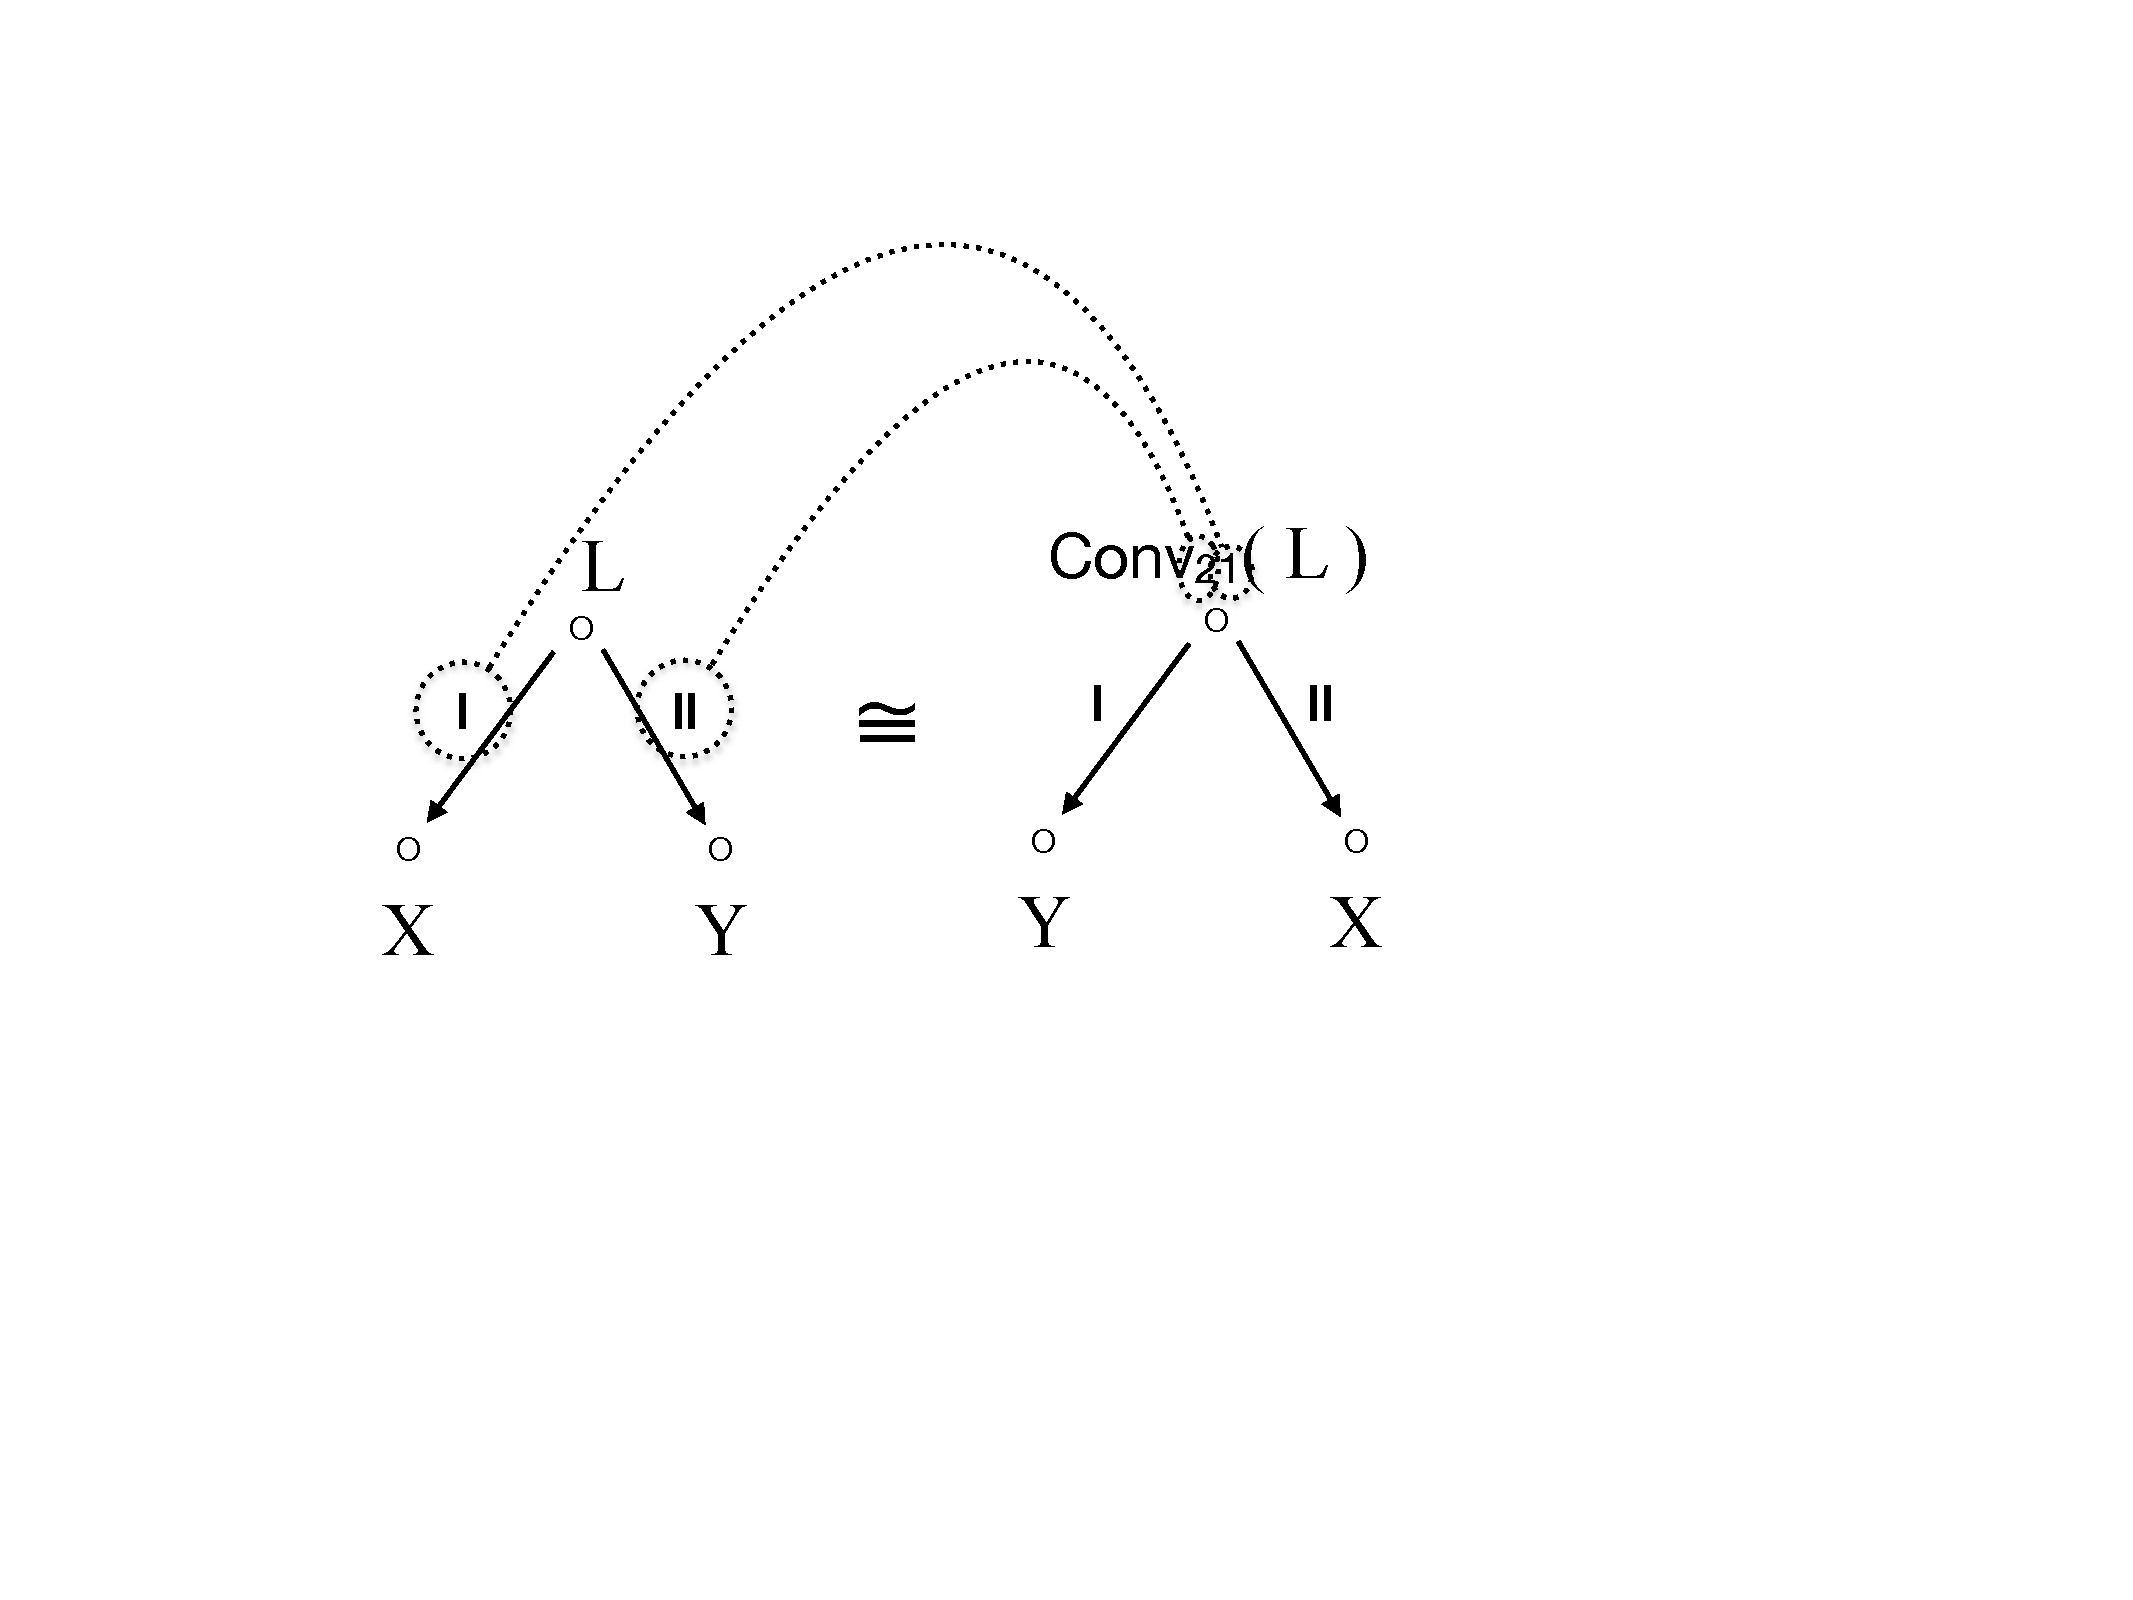
\includegraphics[width=5.5cm]{Fig/ParaLF/CorrSyntPConv-21.pdf}\\
{\small For instance: \textit{X follows Y.}\enskip$\cong$\enskip\textit{Y precedes}\tsub{\lfappl{Conv$_{21}$}{\textit{follow}}} \textit{X.}}
\caption{Correspondence between L's DSyntAs and those of \lfappl{Conv\tsub{21}}{L}}\label{fig:Conv-ijk}
\end{figure}

\begin{longtable*}[l]{ l l >{\raggedright\arraybackslash}p{6.5cm} }

\multicolumn{3}{l}{\textbf{French}} \\

\lfappl{Conv\tsub{21}}{\textit{inclure} \lfgp{X is a set}} & = & \textit{appartenir}\textbf{,} \idiom{\textit{faire partie}} \\
\lfappl{Conv\tsub{3214}}{\textit{prêter}} & = & \textit{emprunter} \\
\multicolumn{3}{l}{\quad\lfgp{N\tsub{X} \textit{prête} N\tsub{Y} \textit{à} N\tsub{Z} \textit{pour la période} N\tsub{W}}} \\
\lfappl{Conv\tsub{3214$\cap$}}{\textit{acheter}} & = & \textit{vendre} \\
\multicolumn{3}{l}{\quad\lfgp{N\tsub{X} \textit{achète} N\tsub{Y} \textit{à} N\tsub{Z} \textit{pour} N\tsub{W}}} \\
\lfappl{Conv\tsub{3214$\cap$}}{\textit{vendre}} & = & \textit{acheter} \\
\lfappl{Conv\tsub{1432$\supset$}}{\textit{acheter}} & = & \textit{payer} \\
\lfappl{Conv\tsub{21}}{\lfgp{\textit{être}} \textit{parent}} & = & \lfgp{\textit{être}} \textit{enfant} \\
\lfappl{Conv\tsub{213}}{\lfgp{\textit{être}} \textit{maître}} & = & \lfgp{\textit{être}} \textit{élève} \lfgp{\textit{du prof. Ménard en math}} \\
\vspace{2pt}\lfappl{Conv\tsub{21}}{\textit{meilleur}} & = & \textit{pire}\vspace{6pt} \\

\multicolumn{3}{l}{\textbf{Russian}} \\

\lfappl{Conv\tsub{21}}{\textit{soder\v{z}at\palati} \lfgp{X is a set}} & = & \textit{prinadle\v{z}at\palati} \\
\lfappl{Conv\tsub{3214}}{\textit{odol\v{z}it\palati}\sensenum{I} \lfgp{N\tsub{\textsc{dat}}}} & = & \textit{odol\v{z}it\palati}\sensenum{II} \lfgp{\textit{u} N\tsub{\textsc{gen}}} \\
\multicolumn{3}{l}{\quad\lfgp{N\tsub{X-\textsc{nom}} \textit{odol\v{z}il} N\tsub{Y-\textsc{acc}} N\tsub{Z-\textsc{dat}} \textit{na vremja} N\tsub{W-\textsc{acc}}}} \\
\lfappl{Conv\tsub{3214$\cap$}}{\textit{kupit\palati}} & = & \textit{prodat\palati} \\
\multicolumn{3}{l}{\quad\lfgp{N\tsub{X-\textsc{nom}} \textit{kupil} N\tsub{Y-\textsc{acc}} \textit{u} N\tsub{Z-\textsc{gen}} \textit{za} N\tsub{W-\textsc{acc}}}} \\
\lfappl{Conv\tsub{3214$\cap$}}{\textit{prodat\palati}} & = & \textit{kupit\palati} \\
\lfappl{Conv\tsub{1432$\supset$}}{\textit{kupit\palati}} & = & \textit{zaplatit\palati} \\
\lfappl{Conv\tsub{21}}{\lfgp{\textit{byt\palati}} \textit{roditelem}} & = & \lfgp{\textit{byt\palati}} \textit{rebënkom} \\
\lfappl{Conv\tsub{213}}{\lfgp{\textit{byt\palati}} \textit{u\v{c}itelem}} & = &\lfgp{\textit{byt\palati}} \textit{u\v{c}enikom} \lfgp{\textit{prof. Menara po matematike}} \\
\lfappl{Conv\tsub{21}}{\textit{tja\v{z}elee}} & = & \textit{leg\v{c}e} \\

\end{longtable*}

\refstepcounter{LFlist}
\subsubsection*{{\small [\arabic{LFlist}]} \lf{Anti} \lfgp{{\scriptsize Latin} *\textit{antonymum}}: antonym}\label{lf:Anti}
\addcontentsline{toc}{subsection}{{\footnotesize [\arabic{LFlist}]} \lf{Anti}: antonym}\index[lf]{Anti@\lf{Anti}|emph}\index[notion]{antonym|emph}

\lfappl{Anti}{L} has a meaning opposite to that of L and is, therefore, a possible substitute for L in the syntactic structure of the utterance with preservation of the meaning, but under the condition that a negation is added to \lfappl{Anti}{L} as illustrated in \Next[a--b].

\begingroup

\ex. \a. Chris was \emph{absent} from the meeting.\\*
         $\equiv$
     \b. Chris was \emph{not present}\tsub{\lfappl{Anti}{\textit{absent}}} at the meeting.

\endgroup

However, such equivalence is valid only for contradictory antonyms\index[notion]{antonym!contradictory [=~complementary] \tld} (see type~\ref{txt:contradictoryAntonym} of antonyms after the illustrations below); with other types of antonyms, the semantic equivalence is only approximate or does not obtain at all. The paraphrastic\index[notion]{paraphrase} relation holding between a lexical unit L and \lfappl{Anti}{L}\thinspace+\thinspace{}Negation is too complex to be summarized here with a single paraphrasing rule, and it is considered below separately for each of the four types of antonyms.

\begin{longtable*}[l]{ l l >{\raggedright\arraybackslash}p{7cm} }

\multicolumn{3}{l}{\textbf{English}} \\*

\lfappl{Anti}{\textit{respect}\tsub{(N)}} & = & \textit{disrespect}\tsub{(N)} \\
\lfappl{Anti}{\textit{small}\tsub{(Adj)}} & = & \textit{big}\tsub{(Adj)} \\
\lfappl{Anti}{\textit{hot}} & = & \textit{cold}\tsub{(Adj)} \\
\lfappl{Anti}{\textit{with}} & = & \textit{without} \\
\lfappl{Anti}{\textit{dress}\tsub{(V)}} & = & \textit{undress}\tsub{(V)} \\
\lfappl{Anti\tsub{$\cap$}}{\textit{build}\tsub{(V)}} & = & \textit{destroy} \\
\vspace{2pt}\lfappl{Anti}{\textit{Yummy!}} & = & \textit{Yuck!} \\[6pt]

\multicolumn{3}{l}{\textbf{French}} \\*

\lfappl{Anti}{\textit{respect}} & = & \textit{irrespect} \\
\lfappl{Anti\tsub{$\supset$}}{\textit{mentionner}} & = & \idiom{\textit{passer sous silence}} \\
\lfappl{Anti}{\textit{petit}\tsub{(Adj)}} & = & \textit{grand}\tsub{(Adj)} \\
\lfappl{Anti}{\textit{chaud}\tsub{(Adj)}} & = & \textit{froid}\tsub{(Adj)} \\
\lfappl{Anti}{\textit{avec}} & = & \textit{sans} \\
\lfappl{Anti}{\textit{habiller}} & = & \textit{déshabiller} \\
\lfappl{Anti\tsub{$\cap$}}{\textit{construire}} & = & \textit{détruire} \\*
\vspace{2pt}\lfappl{Anti}{\textit{Miam !}} & = & \textit{Beurk !}\vspace{6pt} \\

\multicolumn{3}{l}{\textbf{Russian}} \\*

\lfappl{Anti}{\textit{uva\v{z}enie}} & = & \textit{neuva\v{z}enie} \\
\lfappl{Anti\tsub{$\supset$}}{\textit{upomjanut\palati}} & = & \idiom{\textit{obojti mol\v{c}aniem}} \\
\lfappl{Anti}{\textit{malen\palati{}kij}} & = & \textit{bol\palati{}\v{s}oj} \\
\lfappl{Anti}{\textit{gorja\v{c}ij}} & = & \textit{xolodnyj} \\
\lfappl{Anti}{\textit{s}} & = & \textit{bez} \\
\lfappl{Anti}{\textit{odet\palati}} & = & \textit{razdet\palati} \\
\lfappl{Anti\tsub{$\cap$}}{\textit{stroit\palati}} & = & \textit{razru\v{s}at\palati} \\
\lfappl{Anti}{\textit{Ux\onewdf{}ty!}}\footnotemark\index[notion]{wordform} & = & \textit{Fu!} \\

\end{longtable*}\footnotetext{\label{fn:greyUnderscoring}The grey underscoring of the space between two strings of letters, as in \textsc{ux\onewdf{}ty}, shows that, linguistically speaking, this expression is a single wordform, which is traditionally spelled in two words (cf. \textsc{at\onewdf{}all}, \textsc{at\onewdf{}last} or \textsc{by\onewdf{}far}).}

Antonyms come in four types: contradictory, contrary, scalar and positioning antonyms.

\begin{enumerate}

\item \notion{Contradictory} (or~\notion{complementary}) \notion{antonyms}\index[notion]{antonym!contradictory [=~complementary] \tld}\phantomsection\label{txt:contradictoryAntonym}. A contradictory antonym is opposed to its ``partner'' by a negation of the highest level of its meaning, i.e., that applies to the central component of its lexicographic definition\index[notion]{component of a definition!central \tld}\index[notion]{definition!central component of a \tld} \parencite[Sec.~2.4.1]{MelcukPolguere2018}: `\lfappl{Anti}{L}' $=$ `non L'. Two mutually contradictory antonyms represent the two values of a binary category. For instance, \textsc{present}\tsub{(Adj)} \senseex{in a room} is a contradictory antonym of \textsc{absent}\tsub{(Adj)} \senseex{from a room}:

\begin{tabular}{ l l p{7cm} }

`[X] absent from Y' & = & `[X] \emph{not} present in Y' \\

\end{tabular}

Contradictory antonyms do not (or hardly) allow for gradation: *\textit{more}\verythinspace/\verythinspace\textit{less present in a room}. In contrast, the remaining three types of antonyms are gradable.

\item \notion{Contrary antonyms}\index[notion]{antonym!contrary \tld}. Two mutually contrary antonyms are opposed by a negation that is deeply embedded in the lexicographic definition\index[notion]{definition!lexicographic \tld} of one of them, i.e., that applies to a peripheral component\index[notion]{component of a definition!peripheral \tld}\index[notion]{definition!peripheral component of a \tld}. For instance, \textsc{close}\tsub{(V)} \senseex{a door} is a contrary antonym of \textsc{open}\tsub{(V)} \senseex{a door}:

\begin{tabular}{ l l p{7cm} }

`X opens Y' & = & `X causes that Y becomes open\tsub{(Adj)}' \\
`X closes Y' & = & `X causes that Y becomes \emph{not} open\tsub{(Adj)}' \\

\end{tabular}

These semantic decompositions show that `close\tsub{(V)}' $\neq$ `not open\tsub{(V)}' and, therefore, that \textsc{close}\tsub{(V)} and \textsc{open}\tsub{(V)} are not contradictory antonyms.

\item\phantomsection\label{item:scalarAntonym} \notion{Scalar antonyms}\index[notion]{antonym!scalar \tld}. They are opposed by the components `more' $\sim$ `less' in their lexicographic definitions\index[notion]{definition!lexicographic \tld}: `more'\slashs`less' indicates the position on a gradable scale, or on an axis. For instance, \textsc{heavy}\tsub{(Adj)} and \textsc{light}\tsub{(Adj)} are scalar antonyms:

\begin{tabular}{ l l p{7.5cm} }

`X is heavy' & = & `X's weight is \emph{higher} [=~`\emph{more} high'] than the normal weight of Xs' \\
`X is light' & = & `X's weight is \emph{lower} [=~`\emph{less} high'] than the normal weight of Xs' \\

\end{tabular}

The opposition between `more' and `less' is reducible to the opposition by negation \parencite[190]{Melcuk2015a-e}. Note that if two adjectives are scalar antonyms, their comparative degrees are conversives as well; thus, we have `X is heavier than Y' = `Y is lighter than~X'.

\item \notion{Positioning antonyms}\index[notion]{antonym!positioning \tld}. These antonyms denote two opposite spatial or temporal positions (in a literal or metaphorical sense). For instance, \textsc{top}\tsub{(N)} \senseex{the top of the shelves} and \textsc{bottom}\tsub{(N)} \senseex{the bottom of the shelves} are positioning antonyms:

\begin{tabular}{ l l p{7.2cm} }
`top of X' & = & `part of X that is the \emph{furthest} [=~`\emph{least} close'] to the surface on which X is located' \\
`bottom of X' & = & `part of X that is the \emph{closest} [=~`\emph{most} close'] to the surface on which X is located' \\
\end{tabular}

\end{enumerate}

As is seen, all types of antonyms are based on negation. It is the position of negation in the lexicographic definition\index[notion]{definition!lexicographic \tld} of lexical units that are \lfappl{Anti}{L} that determines the type of antonymy. In the enumeration of the four antonym types above, we started with the negation occupying the uppermost position in the definition and concluded with the negation that is the most deeply embedded.

A lexical unit can have antonyms of different types. Such is, for instance, the lexeme \textsc{destroy}, appearing in \Next: 

\begingroup
\small

\ex. They destroyed the bridge. \\
     `They caused that the bridge ceased to exist' = `They caused the bridge to \emph{not}[exist]'

\endgroup

\textsc{destroy} has two antonyms: a contradictory one -- \textsc{spare}\tsub{(V)}, cf. \Next, and a contrary one -- \textsc{build}\tsub{(V)}, cf. \NNext.

\begingroup
\small

\ex. They spared the bridge. \\
         `They \emph{not}[caused that the bridge ceased to exist]'
         
\ex. They built the bridge. \\
         `They caused that the bridge \emph{not}[\emph{not}[exist]]' = `They caused that the bridge exists' \\
         \hphantom{......................................................................................}(`\emph{not}[\emph{not}[exist]]' = `exist')

\endgroup

For all four types of antonyms only one LF is used: \lf{Anti}. Theoretically speaking, it is easy to distinguish the four \lf{Anti} LFs by means of super- or subscripts -- e.g. \lf{Anti\tsup{contrad}}, \lf{Anti\tsup{contrary}}, etc. This is, however, superfluous, since each antonym should have its own lexicographic description -- in particular, its definition -- in a lexicographic model\index[notion]{lexicon!\tld\ model}\index[notion]{model!lexicon \tld}\index[notion]{lexicography}, which allows the user of the model to see the meaning relation\index[notion]{meaning!\tld\ relation}\index[notion]{relation!meaning \tld} between L and \lfappl{Anti}{L}.

Note that the cases where a lexical unit has antonyms of different types are infrequent enough.

\largerpage
Sometimes the negation underlying the antonymy has to be encoded  as such in LF formulas; then the LF \lf{Non}\index[lf]{Non@\lf{Non}|emph} `not' is used. Thus, \lf{Non} -- rather than \lf{Anti} -- combines with semantically empty LFs, such as those that represent support verbs\index[notion]{support verb}\index[notion]{verb!support \tld} (\lf{Oper\tsub{i}}\index[lf]{Operi@\lf{Oper\tsub{i}}}, \lf{Func\tsub{i}}\index[lf]{Funci@\lf{Func\tsub{i}}} and \lf{Labor\tsub{ij}}\index[lf]{Laborij@\lf{Labor\tsub{ij}}}, in \chapref{chap:syntLFs}, \sectref{sec:verbeSupport}). And, from a logical viewpoint, a semantically empty verb cannot have an antonym: an antonym of L is supposed to have an opposite meaning with respect to that of L, while a light verb has no meaning. Therefore, we have:

\begingroup
\small
\ex. \begingroup\setlength{\tabcolsep}{2pt}
\begin{tabular}[t]{ l l >{\raggedright\arraybackslash}p{8cm} }
\lfappl{Oper\tsub{1}}{\textit{consent}\tsub{(N)}} & = & \textit{give}\textbf{,} \textit{grant} \lfgp{\textsc{art} \tld} \\
\lfappl{NonOper\tsub{1}}{\textit{consent}\tsub{(N)}} & = & \textit{refuse} \lfgp{\textsc{art} \tld} \\
\end{tabular}\endgroup

\endgroup

\begin{historicalremark}
The previous presentations of LFs, e.g. \textcite[75--81]{MelcukEtAl1999}, did not introduce the LF \lf{Non} explicitly. In these publications the LF \lf{Non} (as \lf{Non} or \lf{non}) was simply smuggled into complex LF formulas.
\end{historicalremark}

\section{Three LFs related to \lf{Syn} and \lf{Anti}: \lf{Gener}, \lf{Figur}, \lf{Contr}}\label{sec:LFapparenteesSynAnti}

\refstepcounter{LFlist}
\subsubsection*{{\small [\arabic{LFlist}]} \lf{Gener} \lfgp{{\scriptsize Latin} \textit{genus}}: generic term}\label{lf:Gener}
\addcontentsline{toc}{subsection}{{\footnotesize [\arabic{LFlist}]} \lf{Gener}: generic term}\index[lf]{Gener@\lf{Gener}|emph}

\lfappl{Gener}{L} -- a generic term\index[notion]{generic term|emph} for L -- stands for the name of one of the semantic classes\index[notion]{semantic!\tld\ class} to which L's meaning may belong. It applies to L of any PoS and, like \lf{Syn}, it borrows L's PoS:

\begin{quote}
\begingroup
\small
\phantomsection\label{txt:PoSGener}\begin{tabular}{ l c c c c c }
   \midrule
   \multicolumn{6}{l}{\lf{Gener}: borrows L's PoS} \\
   \midrule
   \textbf{L} & V & N & Adj & Adv & Claus \\
   \midrule
   \textbf{\lfappl{Gener}{L}} & V & N & Adj & Adv & Claus\lfgp{?} \\
   \midrule
\end{tabular}
\endgroup
\end{quote}

\index[notion]{government pattern!\tld\ of an LF value element}\index[notion]{value of an LF!government pattern of an element of the \tld}
\begin{longtable*}[l]{ l l >{\raggedright\arraybackslash}p{8cm} }

\multicolumn{3}{l}{\textbf{English}} \\*

\lfappl{Gener}{\textit{love}\tsub{(N)}} & = & \textit{feeling} \lfgp{\textit{of} \tld}\textbf{;} \textit{emotion} \lfgp{\textit{of} \tld} \\%[1pt]
\lfappl{Gener}{\textit{gas}\tsub{(N)}} & = & \lfgp{\textit{gaseous}} \textit{substance} \\
\vspace{2pt}\lfappl{Gener}{\textit{see}\tsub{(V)}} & = & \textit{perceive} \lfgp{\textit{visually}} \\[6pt]

\multicolumn{3}{l}{\textbf{French}} \\*

\lfappl{Gener}{\textit{amour}} & = & \textit{sentiment} \lfgp{\textit{d'}\tld}\textbf{;} \textit{émotion}  \\
\lfappl{Gener}{\textit{gaz}} & = & \textit{substance} \lfgp{\textit{gazeuse}}\\
\vspace{2pt}\lfappl{Gener}{\textit{voir}} & = & \textit{percevoir} \lfgp{\textit{visuellement}} \\[6pt]

\multicolumn{3}{l}{\textbf{Russian}} \\*

\lfappl{Gener}{\textit{ljub\suffixsplit{}ov\palati}} & = & \textit{\v{c}uvstvo} \lfgp{\tld\textit{vi}}\textbf{;} \textit{èmocija} \\
\lfappl{Gener}{\textit{gaz}} & = & \lfgp{\textit{gazoobraznoe}} \textit{ve\v{s}\v{c}estvo} \\
\lfappl{Gener}{\textit{videt\palati}} & = & \textit{vosprinimat\palati} \lfgp{\textit{zritel\palati{}no}} \\

\end{longtable*}

\paragraph*{Identifying \lfappl{Gener}{L}.}

For a lexical unit to belong to the value of \lfappl{Gener}{L} it is necessary and sufficient to appear in the following constructions:

\begin{itemize}

\item for nouns: L\textit{,} L′\textit{,} L′′\textit{, ... and other} \lfappl{Gener}{L} 

\begingroup
\small

\ex. \textit{melons, raspberries, mangoes, ... and other fruits}\tsub{\lfappl{Gener}{\textit{melon}}}

\endgroup

\item for verbs, adjectives and adverbs: L\textit{,} L′\textit{,} L′′\textit{, ... and} \lfappl{Gener}{L} \textit{in other ways}

\begingroup
\small

\ex. \a. \textit{see, smell, ... and perceive}\tsub{\lfappl{Gener}{\textit{see}}} \textit{in other ways}
     \b. \textit{fried, boiled, ... and cooked}\tsub{\lfappl{Gener}{\textit{fried}}} \textit{in other ways}

\endgroup

\end{itemize}

These examples show that \lf{Gener} is a powerful classifier: it identifies numerically important semantic classes\index[notion]{semantic!\tld\ class} of lexical units. For instance:

\begin{itemize}

\item the noun \textsc{dog} is \lf{Gener} of \textsc{basset}, \textsc{bulldog}, \textsc{collie}, \textsc{dachshund}, \textsc{dalmatian}, \idiom{\textsc{german shepherd}}, \textsc{husky}, \textsc{labrador}, \textsc{poodle}, \textsc{setter},~...
    
\item the noun \textsc{feeling}\index[notion]{noun!\tld\ of feeling} is \lf{Gener} of \textsc{adoration}, \textsc{despair}\tsub{(N)}, \textsc{dread}\tsub{(N)}, \textsc{excitement}, \textsc{fear}\tsub{(N)}, \textsc{gratitude}, \textsc{love}\tsub{(N)}, \textsc{remorse}, ...

\end{itemize}

The compatibility of a \lf{Gener} with the above constructions allows for the distinction between \lf{Gener} and \lf{Syn}\tsub{$\subset$}\index[lf]{Syn@\lf{Syn}!\lf{Syn}\tsub{$\subset$}}. Thus, \textsc{dream}\tsub{(N)} is a \lf{Syn}\tsub{$\subset$} of \textsc{nightmare}, rather than a \lf{Gener}, because English does not have an important enough class of lexical units denoting different types of dreams.

\paragraph*{\lf{Gener}-based paraphrasing.}\label{par:GenerBasedParaphrasing}\index[notion]{paraphrase}

The lexical stock and the lexical cooccurrence\index[notion]{cooccurrence, restricted!lexical \tld} of the language allowing, a given \lfappl{Gener}{L} can be used in the two following equivalences grouped under paraphrasing rule \textbf{R\tsub{\lf{Gener}}}:\footnote{These equivalences are described by two distinct paraphrasing rules (Rules~4 and~5) in \textcite[p.\thinspace152]{Melcuk2013c-e}.}

\begin{center}
\phantomsection\label{txt:RParaphGener}\APolbox{11.2cm}{%
\begin{tabular}{ l l l }
\textbf{R\tsub{\lf{Gener}}:} & a) & L\tsub{(N)}\enskip{\small$\equiv$}\enskip\lfappl{Gener}{L\tsub{(N)}}\thinspace\syntRel{R}\thinspace L\tsub{(N)} \vspace{3pt}\\

&
& \begingroup\setlength{\tabcolsep}{0pt}\renewcommand{\arraystretch}{.8}\begin{tabular}{ l }
{\small\textit{anger}\tsub{(N)}\enskip$\equiv$\enskip\textit{feeling}\tsub{\lfappl{Gener}{\textit{anger}$_\text{(N)}$}} \textit{of anger}} \\
{\small\textit{submission}\enskip$\equiv$\enskip\textit{attitude}\tsub{\lfappl{Gener}{\textit{submission}}} \textit{of submission}} \\
{\small\textit{smell}\tsub{(N)}\enskip$\equiv$\enskip\textit{sense}\tsub{\lfappl{Gener}{\textit{smell}$_\text{(N)}$}} \textit{of smell}}
\end{tabular}\endgroup  \vspace{3pt}\\

& b) & L\enskip{\small$\equiv$}\enskip\lfappl{Gener}{L}\thinspace\syntRel{R}\thinspace\lfappl{A\tsub{0}/Adv\tsub{0}/Adv\tsub{1}}{L}  \vspace{3pt}\\

&
& \begingroup\setlength{\tabcolsep}{0pt}\renewcommand{\arraystretch}{.8}\begin{tabular}{ l  }
{\small For L\tsub{(N)}: \textit{anger}\tsub{(N)}\enskip$\equiv$\enskip\textit{angry}\tsub{\lfappl{A\tsub{0}}{\textit{anger}$_\text{(N)}$}} \textit{feeling}\tsub{\lfappl{Gener}{\textit{anger}$_\text{(N)}$}}} \\
{\small For L\tsub{(V)}: \textit{see}\enskip$\equiv$\enskip\textit{perceive}\tsub{\lfappl{Gener}{\textit{see}}} \textit{visually}\tsub{\lfappl{Adv\tsub{1}}{\textit{see}}}} \\
{\small For L\tsub{(Adj)}: \textit{visual}\enskip$\equiv$\enskip\textit{visually}\tsub{\lfappl{Adv\tsub{0}}{\textit{visual}}} \textit{perceptible}\tsub{\lfappl{Gener}{\textit{visual}}}} \\
\end{tabular}\endgroup  \vspace{3pt}\\
\multicolumn{3}{>{\raggedright\arraybackslash}p{10cm}}{{\small See below for the description of the LFs \lf{A\tsub{0}} (\sectref{sec:derivationsStructurales}, [\ref{lf:A0}], p.\thinspace\pageref{lf:A0}), \lf{Adv\tsub{0}} (\sectref{sec:derivationsStructurales}, [\ref{lf:Adv0}], p.\thinspace\pageref{lf:A0}) and \lf{Adv\tsub{1}} (\sectref{sec:derivAdvAct}, [\ref{lf:Adv-i}], p.\thinspace\pageref{lf:Adv-i}).}} \\
\end{tabular}
}
\end{center}\index[notion]{paraphrase!deep-syntactic paraphrasing rule!\textbf{R\tsub{\lf{Gener}}}|emph}\index[lf]{A0@\lf{A\tsub{0}}}\index[lf]{Adv0@\lf{Adv\tsub{0}}}\index[lf]{Advi@\lf{Adv\tsub{i}}!\lf{Adv\tsub{1}}}\index[notion]{relation!deep-syntactic \tld}\index[notion]{actantial relation}\index[notion]{relation!actantial \tld}

In subrules a) and b) above, the deep-syntactic relation~\syntDname{R} on the right-hand side of the equivalence remains unspecified, as it varies according to the semantic valence\index[notion]{valence!semantic \tld} and government pattern\index[notion]{government pattern} of each particular \lfappl{Gener}{L}; for instance:

\begingroup
\small

\ex. \a. \textsc{color}\tsub{(N, `color of X that is Y')}: \textit{the color}\tsub{\lfappl{Gener}{\textit{purple}\tsub{(N)}}}\thinspace\syntRel{II}\thinspace\textit{purple}
     \b. \textsc{feeling}\tsub{(`feeling of X towards Y that is Z')}: \textit{the feeling}\tsub{\lfappl{Gener}{\textit{love}\tsub{(N)}}}\thinspace\syntRel{III}\thinspace\lfgp{\textit{of}} \textit{love}
     \c. \textsc{number}\tsub{(N)}: \textit{the number}\tsub{\lfappl{Gener}{\textit{nine}}}\thinspace\syntRel{ATTR}\thinspace\textit{nine}

\endgroup

\paragraph*{Multiplicity of the values of \lfappl{Gener}{L}.}

A lexical unit L can have multiple elements of the value for \lfappl{Gener}{L}. This happens in two cases.

The first case is trivial. As for any other LF, there can be multiple elements of the value of \lfappl{Gener}{L} that are (quasi-)synonyms; for instance:

\begingroup
\small

\ex. \begingroup\setlength{\tabcolsep}{2pt}
\begin{tabular}[t]{ l l >{\raggedright\arraybackslash}p{8cm} }
\lfappl{Gener}{\textit{fear}\tsub{(N)}} & = & \textit{feeling} \lfgp{\textit{of} \tld}\textbf{;} \textit{emotion} \lfgp{\textit{of} \tld} \\*
& & \lfgp{\lfappl{Syn\tsub{$\supset$}}{\textit{feeling}} = \textit{emotion}} \\*
\lfappl{Gener}{\textit{bin}\tsub{(N)}} & = & \textit{container}\textbf{;} \textit{receptacle} \\*
& & \lfgp{\lfappl{Syn\tsub{$\cap$}}{\textit{container}} = \textit{receptacle}} \\\end{tabular}\endgroup

\endgroup

The second case is more remarkable as it is conditioned by the special character of L's meaning. Two subcases are distinguished:

\begin{itemize}

\item L denotes\index[notion]{denotation} more than one kind of thing and, therefore, L belongs to more than one semantic class\index[notion]{semantic!\tld class}. This phenomenon  corresponds to L's \notion{semantic ambivalence}\index[notion]{ambivalence, semantic}\index[notion]{semantic!\tld\ ambivalence} \parencite{MilicevicPolguere2010-e,SmirnovaTolochin2018}, that is, to the presence of a disjunction in L's definition.\footnote{See also the related notions of \emph{facet}\verythinspace/\verythinspace\emph{subsense} \parencite{Cruse1995} and \emph{logical polysemy} \parencite{Pustejovsky1995}.}

\item  L's definition contains a classifying component -- called \notion{semantic-class marking component}\index[notion]{component of a definition!semantic-class marking \tld} \parencite[Sec.~2.4.1.2]{MelcukPolguere2018} -- that underlies a value of \lfappl{Gener}{L}.   If, at the same time, the central component\index[notion]{definition!central component of a \tld}\index[notion]{component of a definition!central \tld} of L's definition\index[notion]{definition!lexicographic \tld} underlies also a value of \lfappl{Gener}{L}, which is a prototypical case, L obtains more than one type of \lfappl{Gener}{L}.

\end{itemize}

Let us take an example: the definition of the lexeme \textsc{snow}\tsub{(N)}, which illustrates both situations.

\begingroup
\small

\ex. \label{ldef:defSNOW-n}\APolbox{11cm}{%
   \begin{tabular}{ l p{8cm} }
   \textit{snow on Y} :
   &
   frozen water that is falling or has fallen from the sky on geographical place Y \newline
   \setlength{\tabcolsep}{.5pt}\begin{tabular}{ p{0.2cm} >{\raggedright\arraybackslash}p{6cm} }
   \SpecDiff & in the form of white flakes \\
   \end{tabular} \\
   & or \\
   &
   this falling \newline
   \setlength{\tabcolsep}{.5pt}\begin{tabular}{ p{0.2cm} >{\raggedright\arraybackslash}p{6cm} }
   \SpecDiff & which is a weather phenomenon \\
   \end{tabular} \\
%   \multicolumn{2}{|l|}{Ex.: \textit{How is an atom of the \textbf{element} 54 (Xe) likely to act during a chemical reaction?}} \\
\end{tabular}
}

\endgroup

In the above definition, the disjunction in the central component (`or') and the semantic-class marking component (`which is a weather phenomenon') combine to produce two types of \lfappl{Gener}{\textit{snow}\tsub{(N)}}:

\begingroup
\small

\ex. \begingroup\setlength{\tabcolsep}{2pt}
\begin{tabular}[t]{ l l >{\raggedright\arraybackslash}p{7cm} }
\lfappl{Gener}{\textit{snow}\tsub{(N)}} & = & (i)\hspace{3pt} \textit{substance}\textbf{;} \\*
& & (ii) \textit{precipitation}\textbf{,} \idiom{\textit{weather condition}} \\
\end{tabular}\endgroup

\endgroup

Formula \Last presupposes that we are dealing with one single sense of \textsc{snow}\tsub{(N)}, that is, with one lexeme, and not with a case of polysemy\index[notion]{polysemy}, that is, with two lexemes -- one denoting\index[notion]{denotation} a substance and one denoting the event of its falling. This can be demonstrated using the \emph{Unifying cooccurrence}\index[notion]{cooccurrence, restricted} criterion presented in \textcite[Ch.~11, Sec.~3.2.2]{Melcuk2013c-e}. Indeed, a given occurrence of \textit{snow}\tsub{(N)} in an utterance can be used to refer to both substance and event simultaneously:

\begingroup
\small

\ex. The snow that \emph{started} \lfgp{snow as precipitation} this morning \\
     \hphantom{.....}is beautifully \emph{fluffy} \lfgp{snow as substance}.

\endgroup

For this reason, both types of denotation of \textsc{snow}\tsub{(N)} (substance and meteorological event) have to be considered as belonging to one lexical unit, with a disjunctive central component\index[notion]{definition!lexicographic \tld}\index[notion]{definition!disjunctive central component of a \tld}\index[notion]{component of a definition!disjunctive central \tld} in its definition.

 The classifying power of \lf{Gener} makes this LF particularly important in the structuring of natural language lexical networks\index[notion]{lexical network}\index[notion]{network \lfgp{see also \textit{graph}}!lexical \tld} and in the description of lexical regularities\index[notion]{regularity} -- see \chapref{chap:NotionLF}, \sectref{sec:generalizationsGener}.
 
\begin{furtherreading}
For more on generic terms and lexicographic definitions, see \textcite[Sec.~3]{Polguere2022a} and \textcite{Goddard2017}.
\end{furtherreading}

\refstepcounter{LFlist}
\subsubsection*{{\small [\arabic{LFlist}]} \lf{Figur} \lfgp{{\scriptsize Latin} \textit{figuraliter} `figuratively'}: figurative term}\label{lf:Figur}
\addcontentsline{toc}{subsection}{{\footnotesize [\arabic{LFlist}]} \lf{Figur}: figurative term}\index[lf]{Figur@\lf{Figur}|emph}

\lfappl{Figur}{L} is a metaphorical expression having the same meaning as the noun L plus a somehow artistic representation of L; it is either a lexical unit or a collocation whose base is L and the collocate, a noun that takes L as its DSyntA\thinspace\syntDname{I}. The relation of paraphrase between L and \lfappl{Figur}{L} is accounted for by the \textbf{R\tsub{\lf{Figur}}}\index[notion]{paraphrase!deep-syntactic paraphrasing rule!\textbf{R\tsub{\lf{Figur}}}|emph} paraphrasing rule:

\begin{center}
\phantomsection\label{txt:RParaphFigur}\APolbox{3.7cm}{%
\textbf{R\tsub{\lf{Figur}}:}\quad L\enskip{\small$\cong$}\enskip\lfappl{Figur}{L}
}
\end{center}

The equivalence established by this rule is approximate because the use of \lfappl{Figur}{L} necessarily adds to the meaning of L a rhetorical content, as illustrated by \Next[a--b]:

\begingroup
\small

\ex. \a. He never experienced \emph{passion}.\\
         $\cong$
     \b. He never experienced the \emph{flame of passion}\tsub{\lfappl{Figur}{\textit{passion}}}.

\endgroup

\begin{quote}
\begingroup
\small
\begin{tabular}{ l c }
   \midrule
   \multicolumn{2}{ l }{\lf{Figur}: nominal} \\
   \midrule
   \textbf{L} & N \\
   \midrule
   \textbf{\lfappl{Figur}{L}} & N \\
   \midrule
\end{tabular}
\endgroup
\end{quote}

Being a figurative \emph{substitute} explains the status of \lf{Figur} as a paradigmatic (rather than syntagmatic) LF\index[notion]{lexical function!paradigmatic vs. syntagmatic \tlds}. It is used for stylistic effects, and for this reason it is close to the syntagmatic LF \lf{Epit} -- \chapref{chap:syntLFs}, [\ref{lf:Epit}], p.\thinspace\pageref{lf:Epit}\index[lf]{Epit@\lf{Epit}}. See also the remark on the syntactic similarity of \lf{Figur} to two other syntagmatic LFs: \lf{Germ}\index[lf]{Germ@\lf{Germ}} and \lf{Culm}\index[lf]{Culm@\lf{Culm}} -- \chapref{chap:syntLFs}, [\ref{lf:Germ}--\ref{lf:Culm}], p.\thinspace\pageref{txt:Figur-Germ-Culm}.

\index[notion]{government pattern!\tld\ of an LF value element}\index[notion]{value of an LF!government pattern of an element of the \tld}\index[notion]{cooccurrence, restricted}
\begin{longtable*}[l]{ l l >{\raggedright\arraybackslash}p{7cm} }

\multicolumn{3}{l}{\textbf{English}} \\*

\lfappl{Figur}{\lfgp{bubonic} \textit{plague}\tsub{(N)}} & = & \idiom{\textit{Black Death}}  \\
\lfappl{Figur}{\textit{power}\tsub{(N)}} & = & \textit{reins of} \tld  \\
\lfappl{Figur}{\textit{passion}} & = & \textit{flame of} \tld \\
\lfappl{Figur}{\textit{fog}\tsub{(N)}} & = & \textit{curtain of} \tld\vspace{6pt} \\

\multicolumn{3}{l}{\textbf{French}} \\*

\lfappl{Figur}{\textit{pétrole}} & = & \idiom{\textit{or noir}} \\
\lfappl{Figur}{\textit{pouvoir}} & = & \textit{rênes du} \tld \\
\lfappl{Figur}{\textit{passion}} & = & \textit{flamme de la} \tld \\
\lfappl{Figur}{\textit{brouillard}} & = & \textit{rideau de} \tld\vspace{6pt} \\

\multicolumn{3}{l}{\textbf{Russian}} \\*

\lfappl{Figur}{\textit{vlast\palati}} & = & \idiom{\textit{brazdy pravlenija}} \\
\lfappl{Figur}{\textit{strast\suffixsplit{}\palati}} & = & \textit{plamja} \tld\textit{i} \\
\lfappl{Figur}{\textit{tuman}} & = & \textit{pelena} \tld\textit{a} \\

\end{longtable*}

\refstepcounter{LFlist}
\subsubsection*{{\small [\arabic{LFlist}]} \lf{Contr} \lfgp{{\scriptsize Latin} \textit{contrarium}}: contrastive term}\label{lf:Contr}
\addcontentsline{toc}{subsection}{{\footnotesize [\arabic{LFlist}]} \lf{Contr}: contrastive term}\index[lf]{Contr@\lf{Contr}|emph}

\lfappl{Contr}{L} is a lexical entity that expresses a meaning that is in contrastive opposition with that of L, while not being an \lf{Anti} of the latter.

The contrastive opposition of L and the value of \lfappl{Contr}{L} is not just conceptual, but truly lexical -- i.e., language-dependent. In particular, it has to be manifested in phrasemes\index[notion]{phraseme} of the language, such as the italicized idiom in \Next below for \textsc{ice}\tsub{(N)} and its \lf{Contr} \textsc{fire}\tsub{(N)}.

\begingroup
\small

\ex. They are \emph{\idiom{like ice and fire}}, but friends nonetheless.

\endgroup

\begin{quote}
\begingroup
\small
\begin{tabular}{ l c c c c c}
   \midrule
   \multicolumn{6}{l}{\lf{Contr}: borrows L's PoS} \\
   \midrule
    \textbf{L} & V & N & Adj & Adv & Claus \\
   \midrule
   \textbf{\lfappl{Contr}{L}} & V & N & Adj & Adv & Claus \\
   \midrule
\end{tabular}
\endgroup
\end{quote}

\begin{longtable*}[l]{ l l >{\raggedright\arraybackslash}p{7cm} }

\multicolumn{3}{l}{\textbf{English}} \\*

\lfappl{Contr}{\textit{sea}} & = & \textit{land}\tsub{(N)}  \\
\lfappl{Contr}{\textit{ice}\tsub{(N)}} & = & \textit{fire}\tsub{(N)}  \\
\lfappl{Contr}{\textit{black}\tsub{(Adj)}} & = & \textit{white}\tsub{(Adj)}  \\
\lfappl{Contr}{\textit{here}} & = & \textit{there}\vspace{6pt}  \\

\multicolumn{3}{l}{\textbf{French}} \\*

\lfappl{Contr}{\textit{manger}\tsub{(V)}} & = & \textit{boire}\tsub{(V)} \\
\lfappl{Contr}{\textit{terre}} & = & \textit{mer} \\
\lfappl{Contr}{\textit{eau}} & = & \textit{feu} \\
\lfappl{Contr}{\textit{nous}} & = & \textit{eux} \\
\lfappl{Contr}{\textit{noir}\tsub{(Adj)}} & = & \textit{blanc}\tsub{(Adj)} \\
\lfappl{Contr}{\textit{ici}} & = & \textit{là}\vspace{6pt} \\

\multicolumn{3}{l}{\textbf{Russian}} \\*

\lfappl{Contr}{\textit{more}} & = & \textit{su\v{s}a} \\
\lfappl{Contr}{\textit{lëd}} & = & \textit{plamen\palati} \\
\lfappl{Contr}{\textit{my}} & = & \textit{oni} \\
\lfappl{Contr}{\textit{\v{c}ërnyj}} & = & \textit{belyj} \\
\lfappl{Contr}{\textit{zdes\palati}} & = & \textit{tam} \\

\end{longtable*}

\section{Structural, i.e. syntactically motivated, derivatives}\label{sec:derivationsStructurales}

The following five LFs -- \lf{S\tsub{0}}, \lf{V\tsub{0}}, \lf{A\tsub{0}}, \lf{Adv\tsub{0}} and \lf{Claus\tsub{0}} -- represent the five possible derivations that modify L's deep part of speech\index[notion]{part of speech [PoS]!deep \tld}, but do not entail semantic increments to L: nominalization, verbalization, adjectivization, adverbialization and clausativization. The ``\lf{\tsub{0}}'' subscript in the name of these LFs indicates that they are structural (purely syntactic) derivatives.

\refstepcounter{LFlist}
\subsubsection*{{\small [\arabic{LFlist}]} \lf{S\tsub{0}} \lfgp{{\scriptsize Latin} \textit{substantivum}}: nominalization}\label{lf:S0}
\addcontentsline{toc}{subsection}{{\footnotesize [\arabic{LFlist}]} \lf{S\tsub{0}}: nominalization}\index[lf]{S0@\lf{S\tsub{0}}|emph}

\lf{S\tsub{0}} applies to a non-nominal lexical unit L and returns a noun having the same meaning as L.

\begin{quote}
\begingroup
\small 
\begin{tabular}{ l c c c c }
   \midrule
   \multicolumn{5}{l}{\lf{S\tsub{0}}: nominal} \\
   \midrule
   \textbf{L} & V & Adj & Adv & Claus \\
   \midrule
   \textbf{\lfappl{S\tsub{0}}{L}} & N & N & N & N \\
   \midrule
\end{tabular}
\endgroup
\end{quote}

\begin{longtable*}[l]{ l l >{\raggedright\arraybackslash}p{7cm} }

\multicolumn{3}{l}{\textbf{English}} \\*

\lfappl{S\tsub{0}}{\textit{present}\tsub{(V)}} & = & \textit{presentation}  \\
\lfappl{S\tsub{0}}{\textit{leave}\tsub{(V)}} & = & \textit{departure}  \\
\lfappl{S\tsub{0}}{\textit{fall}\tsub{(V)}} & = & \textit{fall}\tsub{(N)}  \\
\lfappl{S\tsub{0}}{\textit{close}\tsub{(Adj)}} & = & \textit{proximity}  \\*
\lfappl{S\tsub{0}}{\textit{Bang!}} & = & \textit{gunshot}\vspace{6pt}  \\

\multicolumn{3}{l}{\textbf{French}} \\*

\lfappl{S\tsub{0}}{\textit{présenter}} & = & \textit{présentation} \\
\lfappl{S\tsub{0}}{\textit{partir}} & = & \textit{départ} \\
\lfappl{S\tsub{0}}{\textit{tomber}} & = & \textit{chute} \\
\lfappl{S\tsub{0}}{\textit{proche}} & = & \textit{proximité} \\
\lfappl{S\tsub{0}}{\textit{près}} & = & \textit{proximité} \\
\lfappl{S\tsub{0}}{\textit{Pan !}} & = & \idiom{\textit{coup de feu}}\vspace{6pt} \\

\multicolumn{3}{l}{\textbf{Russian}} \\*

\lfappl{S\tsub{0}}{\textit{predstavljat\palati}} & = & \textit{predstavlenie} \\
\lfappl{S\tsub{0}}{\textit{uez\v{z}at\palati}} & = & \textit{ot\palati\palat{}ezd} \\
\lfappl{S\tsub{0}}{\textit{padat\palati}} & = & \textit{padenie} \\
\lfappl{S\tsub{0}}{\textit{blizkij}} & = & \textit{blizost\palati} \\
\lfappl{S\tsub{0}}{\textit{rjadom}} & = & \textit{blizost\palati} \\
\lfappl{S\tsub{0}}{\uslabel{child language} \textit{Pif-paf!}} & = & \textit{vystrel} \\

\end{longtable*}

\refstepcounter{LFlist}
\subsubsection*{{\small [\arabic{LFlist}]} \lf{V\tsub{0}} \lfgp{{\scriptsize Latin} \textit{verbum}}: verbalization}\label{lf:V0}
\addcontentsline{toc}{subsection}{{\footnotesize [\arabic{LFlist}]} \lf{V\tsub{0}}: verbalization}\index[lf]{V0@\lf{V\tsub{0}}|emph}

\lf{V\tsub{0}} applies to a non-verbal lexical unit L and returns a verb having the same meaning as L.

\begin{quote}
\begingroup
\small
\begin{tabular}{ l c c c c }
   \midrule
   \multicolumn{5}{l}{\lf{V\tsub{0}}: verbal} \\
   \midrule
   \textbf{L} & N & Adj & Adv & Claus \\
   \midrule
   \textbf{\lfappl{V\tsub{0}}{L}} & V & V & V & V \\
   \midrule
\end{tabular}
\endgroup
\end{quote}

Obviously, only lexical units being genuine predicates\index[notion]{predicate, semantic} -- i.e., denoting facts\index[notion]{fact@`fact'} -- can have a \lf{V\tsub{0}}.

\begin{longtable*}[l]{ l l >{\raggedright\arraybackslash}p{7cm} }

\multicolumn{3}{l}{\textbf{English}} \\*

\lfappl{V\tsub{0}}{\textit{presentation}} & = & \textit{present}\tsub{(V)}  \\
\lfappl{V\tsub{0}}{\textit{oath}} & = & \textit{swear}\tsub{(V)}  \\
\lfappl{V\tsub{0}}{\textit{compliment}\tsub{(N)}} & = & \textit{compliment}\tsub{(V)}  \\
\lfappl{V\tsub{0}}{\textit{age}\tsub{(N)}} & = & \textit{be} \lfgp{NUM\thinspace$+$\thinspace{}N}\tsub{Y} \textit{old} \lfconstr{N denotes a time unit -- e.g., \textsc{month}, \textsc{year}, \textsc{century}} \senseex{She is 33 years old.}  \\
\lfappl{V\tsub{0}}{\textit{stinking}\tsub{(Adj)}} & = & \textit{stink}\tsub{(V)}  \\
\lfappl{V\tsub{0}}{\textit{energetic}} & = & \uslabel{colloquial} \idiom{\textit{be full of beans}}  \\
\lfappl{V\tsub{0}}{\textit{impatient}} & = & \uslabel{colloquial} \idiom{\textit{champ at the bit}}  \\
\lfappl{V\tsub{0}}{\textit{Bang!}} & = & \textit{fire}\tsub{(V)}  \\
\lfappl{V\tsub{0}}{\textit{Wow!}} & = & \textit{be impressed} \vspace{6pt} \\

\multicolumn{3}{l}{\textbf{French}} \\*

\lfappl{V\tsub{0}}{\textit{présentation}} & = & \textit{présenter} \\
\lfappl{V\tsub{0}}{\textit{serment}} & = & \textit{jurer} \\
\lfappl{V\tsub{0}}{\textit{erreur}} & = & \textit{se tromper} \\
\lfappl{V\tsub{0}}{\textit{âge}} & = & \textit{avoir} \lfgp{NUM\thinspace$+$\thinspace{}N}\tsub{Y} \lfconstr{N denotes a time unit -- e.g., \textsc{mois}, \textsc{an}, \textsc{siècle}} \senseex{Elle a 33 ans.} \\
\lfappl{V\tsub{0}}{\uslabel{colloquial} \textit{puant}} & = & \uslabel{colloquial} \textit{puer} \\
\lfappl{V\tsub{0$\supset$}}{\textit{énergique}} & = & \uslabel{colloquial} \idiom{\textit{avoir bouffé du lion}} \\
\lfappl{V\tsub{0}}{\textit{impatient}} & = & \textit{s'impatienter}\textbf{;} \idiom{\textit{prendre le mors aux dents}}\textbf{,} \idiom{\textit{ronger son frein}} \\
\lfappl{V\tsub{0}}{\textit{Pan !}} & = & \idiom{\textit{faire feu}} \\
\lfappl{V\tsub{0}}{\textit{Waouh !}} & = & \textit{être en admiration} \vspace{6pt} \\

\multicolumn{3}{l}{\textbf{Russian}} \\*

\lfappl{V\tsub{0}}{\textit{predstavlenie}} & = & \textit{predstavljat\palati} \\
\lfappl{V\tsub{0}}{\textit{kljatva}} & = & \textit{pokljast\palati{}sja} \\
\lfappl{V\tsub{0}}{\textit{o\v{s}ibka}} & = & \textit{o\v{s}ibit\palati{}sja} \\
\lfappl{V\tsub{0}}{\textit{vozrast}} & = & \lfgp{N\tsub{X-\textsc{dat}}} \textit{byt\palati} \lfgp{NUM\thinspace$+$\thinspace{}N}\tsub{Y} \lfconstr{N denotes a time unit -- e.g., \textsc{mesjac}, \textsc{god}, \textsc{vek}} \senseex{Ej 33 goda.} \\
\lfappl{V\tsub{0}}{\textit{vonju\v{c}ij}} & = & \textit{vonjat\palati} \\
\lfappl{V\tsub{0$\supset$}}{\textit{s\v{c}astlivyj}} & = & \idiom{\textit{byt\palati na sed\palati{}mom nebe}} \\
\lfappl{V\tsub{0}}{\uslabel{child language} \textit{Pif-paf!}} & = & \textit{vystrelit\palati} \\
\lfappl{V\tsub{0}}{\textit{Ux\onewdf{}ty!}} & = & \textit{byt\palati{} v vostorge} \\

\end{longtable*}

\refstepcounter{LFlist}
\subsubsection*{{\small [\arabic{LFlist}]} \lf{A\tsub{0}} \lfgp{{\scriptsize Latin} \textit{adjectivum}}: adjectivization}\label{lf:A0}
\addcontentsline{toc}{subsection}{{\footnotesize [\arabic{LFlist}]} \lf{A\tsub{0}}: adjectivization}\index[lf]{A0@\lf{A\tsub{0}}|emph}

\lf{A\tsub{0}} applies to a non-adjectival lexical unit L and returns an adjective having the same meaning as L.

\begin{quote}
\begingroup
\small
\begin{tabular}{ l c c c c }
   \midrule
   \multicolumn{5}{l}{\lf{A\tsub{0}}: adjectival} \\
   \midrule
   \textbf{L} & V & N & Adv & Claus \\
   \midrule
   \textbf{\lfappl{\lf{A\tsub{0}}}{L}} & Adj & Adj & Adj & Adj \\
   \midrule
\end{tabular}
\endgroup
\end{quote}

\begin{longtable*}[l]{ l l >{\raggedright\arraybackslash}p{7cm} }

\multicolumn{3}{l}{\textbf{English}} \\*

\lfappl{A\tsub{0}}{\textit{compare}} & = & \textit{comparative} \\
\lfappl{A\tsub{0}}{\textit{time}\tsub{(N)}} & = & \textit{temporal} \\
\lfappl{A\tsub{0}}{\textit{school}\tsub{(N)}} & = & \textit{scholar} \\
\lfappl{A\tsub{0}}{\textit{rotation}} & = & \textit{gyratory} \\
\lfappl{A\tsub{0}}{\textit{rapidly}} & = & \textit{rapid}\tsub{(Adj)} \\
\lfappl{A\tsub{0}}{\textit{closely}} & = & \textit{close}\tsub{(Adj)}\vspace{6pt} \\

\multicolumn{3}{l}{\textbf{French}} \\*

\lfappl{A\tsub{0}}{\textit{comparer}} & = & \textit{comparatif} \\
\lfappl{A\tsub{0}}{\textit{temps}} & = & \textit{temporel} \\
\lfappl{A\tsub{0}}{\textit{port}} & = & \textit{portuaire} \\
\lfappl{A\tsub{0}}{\textit{rotation}} & = & \textit{giratoire} \\
\lfappl{A\tsub{0}}{\textit{rapidement}} & = & \textit{rapide}\tsub{(Adj)} \\
\lfappl{A\tsub{0}}{\textit{près}} & = & \textit{proche}\vspace{6pt} \\
% Trouver un A0 d'un clausatif

\multicolumn{3}{l}{\textbf{Russian}} \\*

\lfappl{A\tsub{0}}{\textit{sravnivat\palati}} & = & \textit{sravnitel\palati{}nyj} \\
\lfappl{A\tsub{0}}{\textit{vremja}} & = & \textit{vremennoj} \\
\lfappl{A\tsub{0}}{\textit{port}} & = & \textit{portovyj} \\
\lfappl{A\tsub{0}}{\textit{vra\v{s}\v{c}enie}} & = & \textit{vra\v{s}\v{c}atel\palati{}nyj} \\
\lfappl{A\tsub{0}}{\textit{bystro}} & = & \textit{bystryj} \\
\lfappl{A\tsub{0}}{\textit{rjadom}} & = & \textit{blizkij} \\

\end{longtable*}

\phantomsection\label{txt:A0NonPurelyStructural}Contrary to \lfappl{S\tsub{0}}{L} and \lfappl{V\tsub{0}}{L},
the LF application \lfappl{A\tsub{0}}{L} returns an adjective that does not have \emph{exactly} the same meaning as L. This is so for the following reason. \lfappl{A\tsub{0}}{L} is used as adjectival modifier of a noun, for instance \textit{the temporal coordinate} means `the coordinate relative to time',\footnote{On the lexicographic definition of \lf{A\tsub{0}} lexical units, see \textcite[Sec.~4.1.1]{MelcukPolguere2018}.}\index[notion]{definition!lexicographic \tld} and the syntactic relation of modification (deep-syntactic relation \syntDname{ATTR}\index[notion]{ATTR@\syntDname{ATTR}}) between the lexemes \textsc{coordinate} and \textsc{temporal} [=~\lfappl{A\tsub{0}}{\textit{time}}] expresses the semanteme `relative \lfgp{to}', which connects `coordinate' and `time', as shown in \figref{fig:Ch5-valeurSensA0}.

\begin{figure}

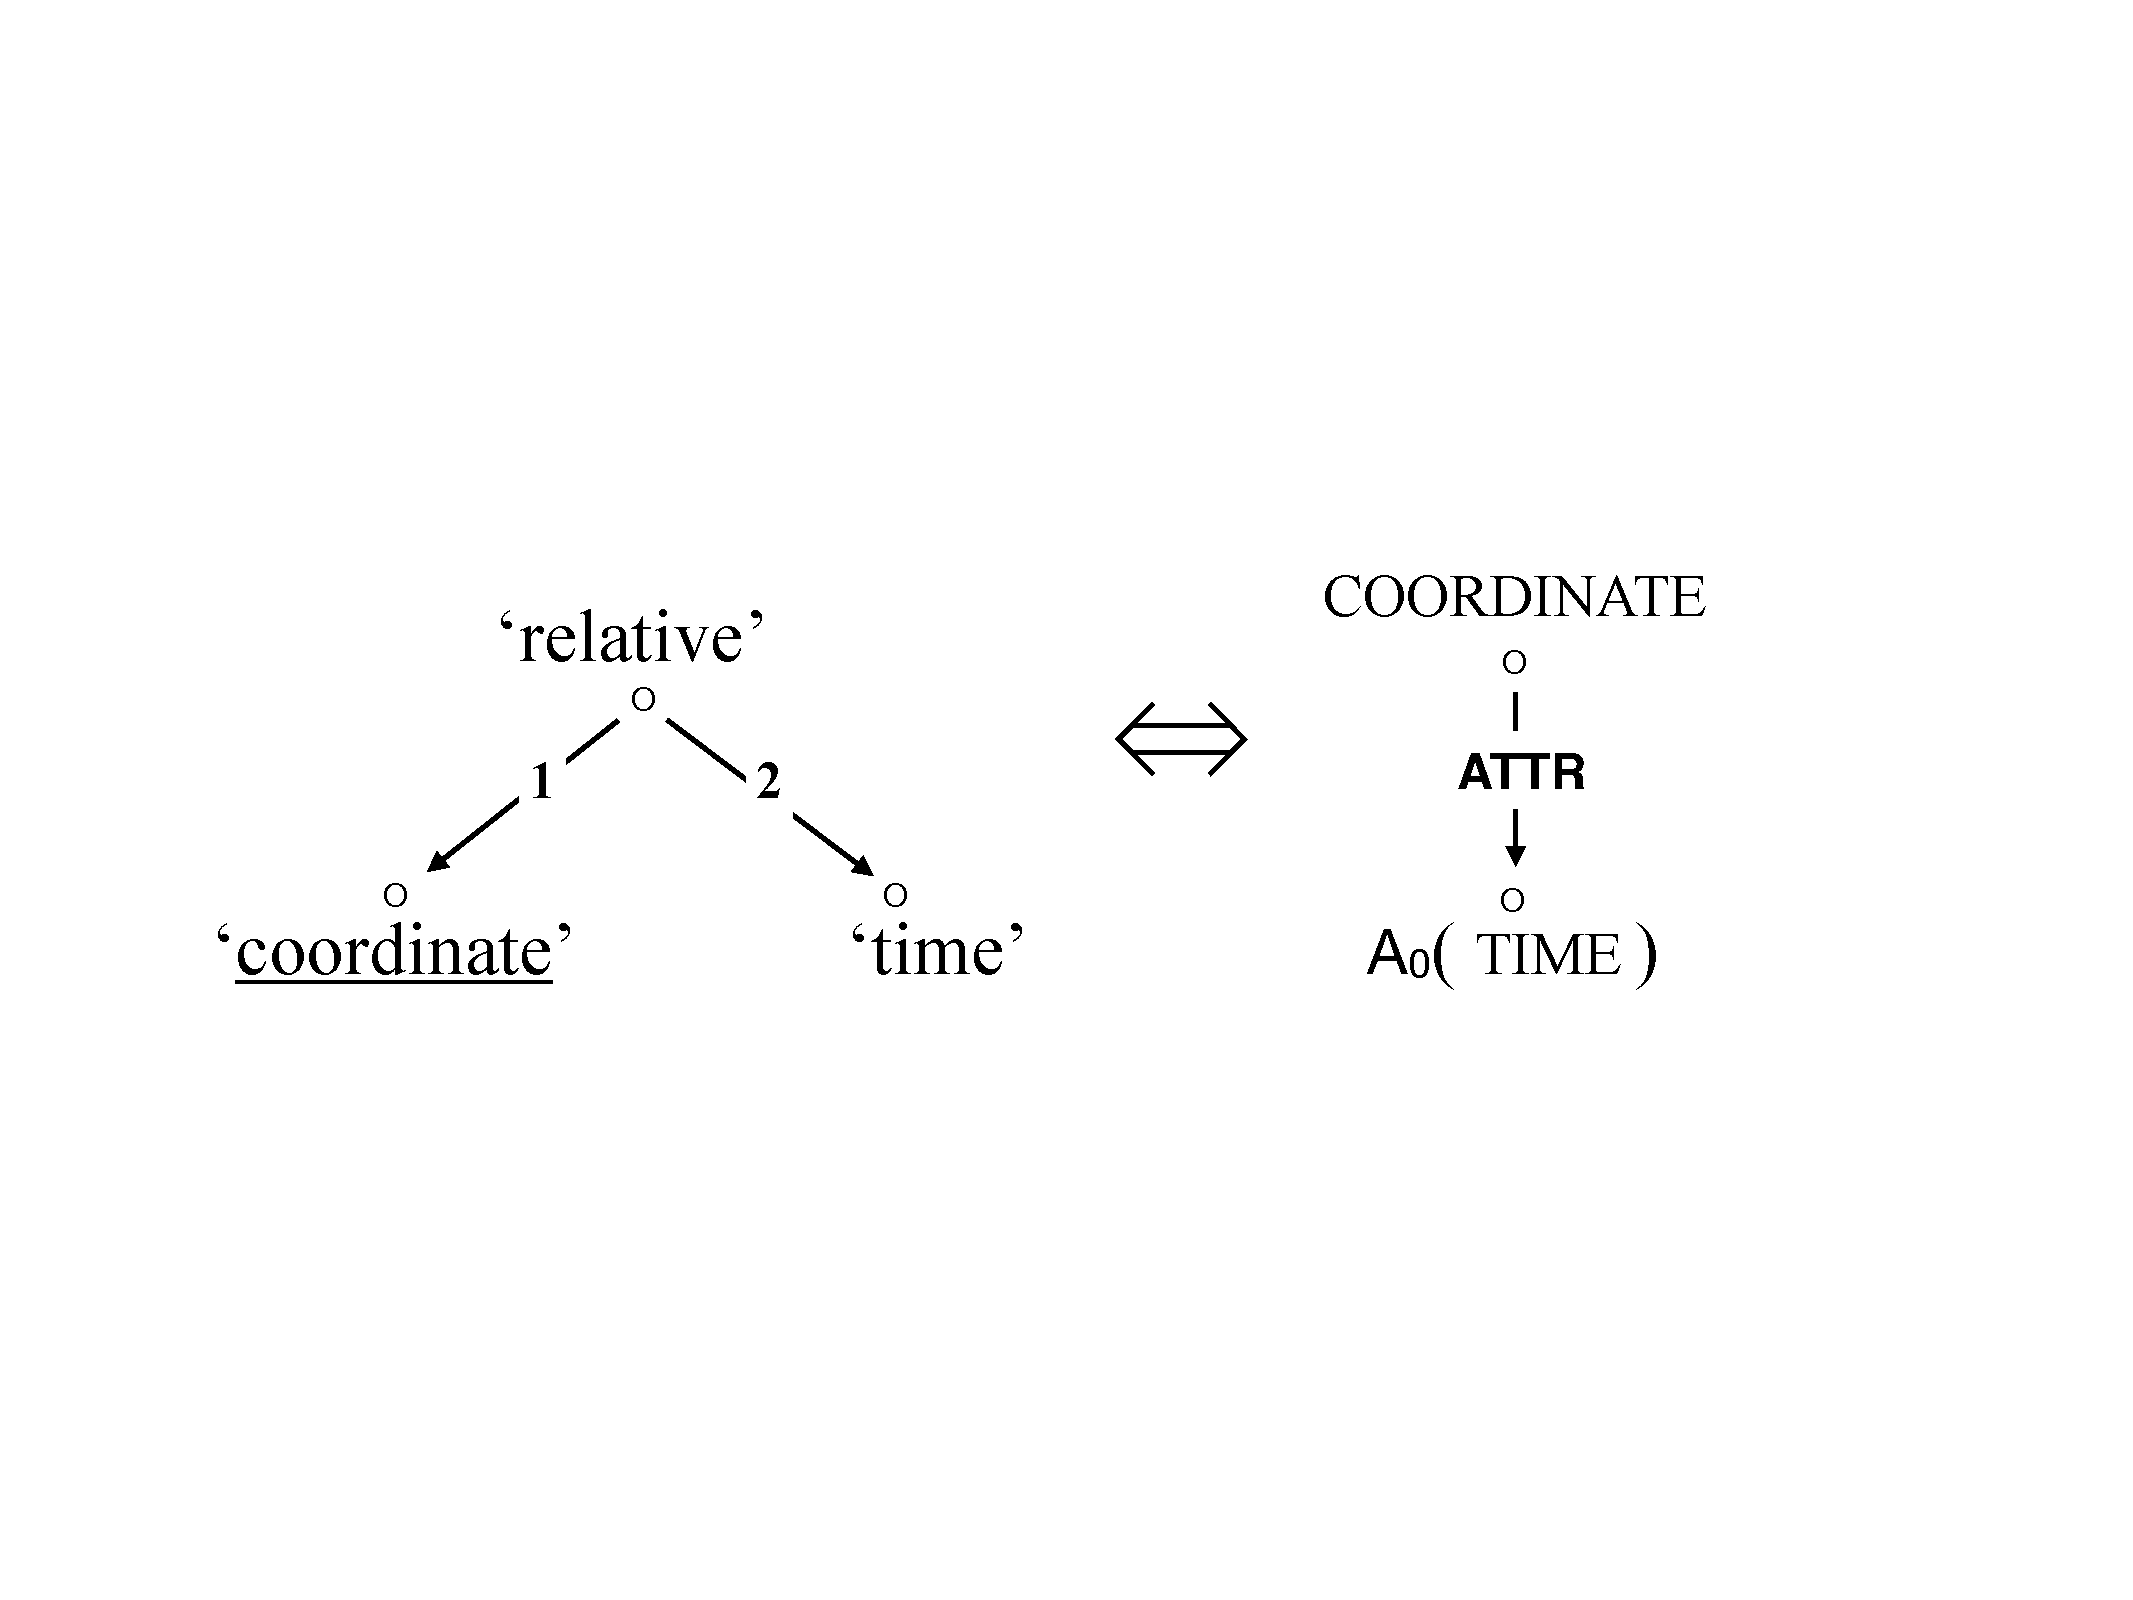
\includegraphics[width=7.3cm]{Fig/ParaLF/SemSyntA0.pdf}
\caption{Semantic content carried by an \lf{A\tsub{0}} syntactic modifier}\label{fig:Ch5-valeurSensA0}
\end{figure}

The semanteme `relative \lfgp{to}' is always included in the meaning of \lf{A\tsub{0}}. Given this semantic increment, it is not the case that \textsc{time}\tsub{(N)} is \lf{S\tsub{0}} of \textsc{temporal}; the \lf{S\tsub{0}} of \textsc{temporal} is \textsc{temporality}. The correspondences between these three lexemes are illustrated in paraphrases\index[notion]{paraphrase} \Next[a--c].

\begingroup
\small

\ex. \a. We measure the dimension of existence relative to \emph{time}.
     \b. We measure the \emph{temporal} dimension of existence.
     \c. We measure the dimension of existence relative to its \emph{temporality}.

\endgroup

The LF that associates \textsc{temporal} to \textsc{temporality} is called \lf{A\tsub{1}} -- an adjective characterizing the first deep-syntactic actant of L (that is, of \textsc{temporality}): \lfappl{A\tsub{1}}{\textsc{temporality}} = \textsc{temporal}. The LF \lf{A\tsub{1}} is presented below (\sectref{sec:derivAdjAct}, [\ref{lf:A-i}], p.\thinspace\pageref{lf:A-i}).

The lexical triplet {\scshape time}\tsub{(N)}, {\scshape temporal} and {\scshape temporality} forms a configuration of lexical links that is visualized in \figref{fig:configA0S0A1}. This type of configuration is highly recurrent in the lexical network\index[notion]{lexical network}\index[notion]{network \lfgp{see also \textit{graph}}!lexical \tld} of English and other languages.

\begin{figure}

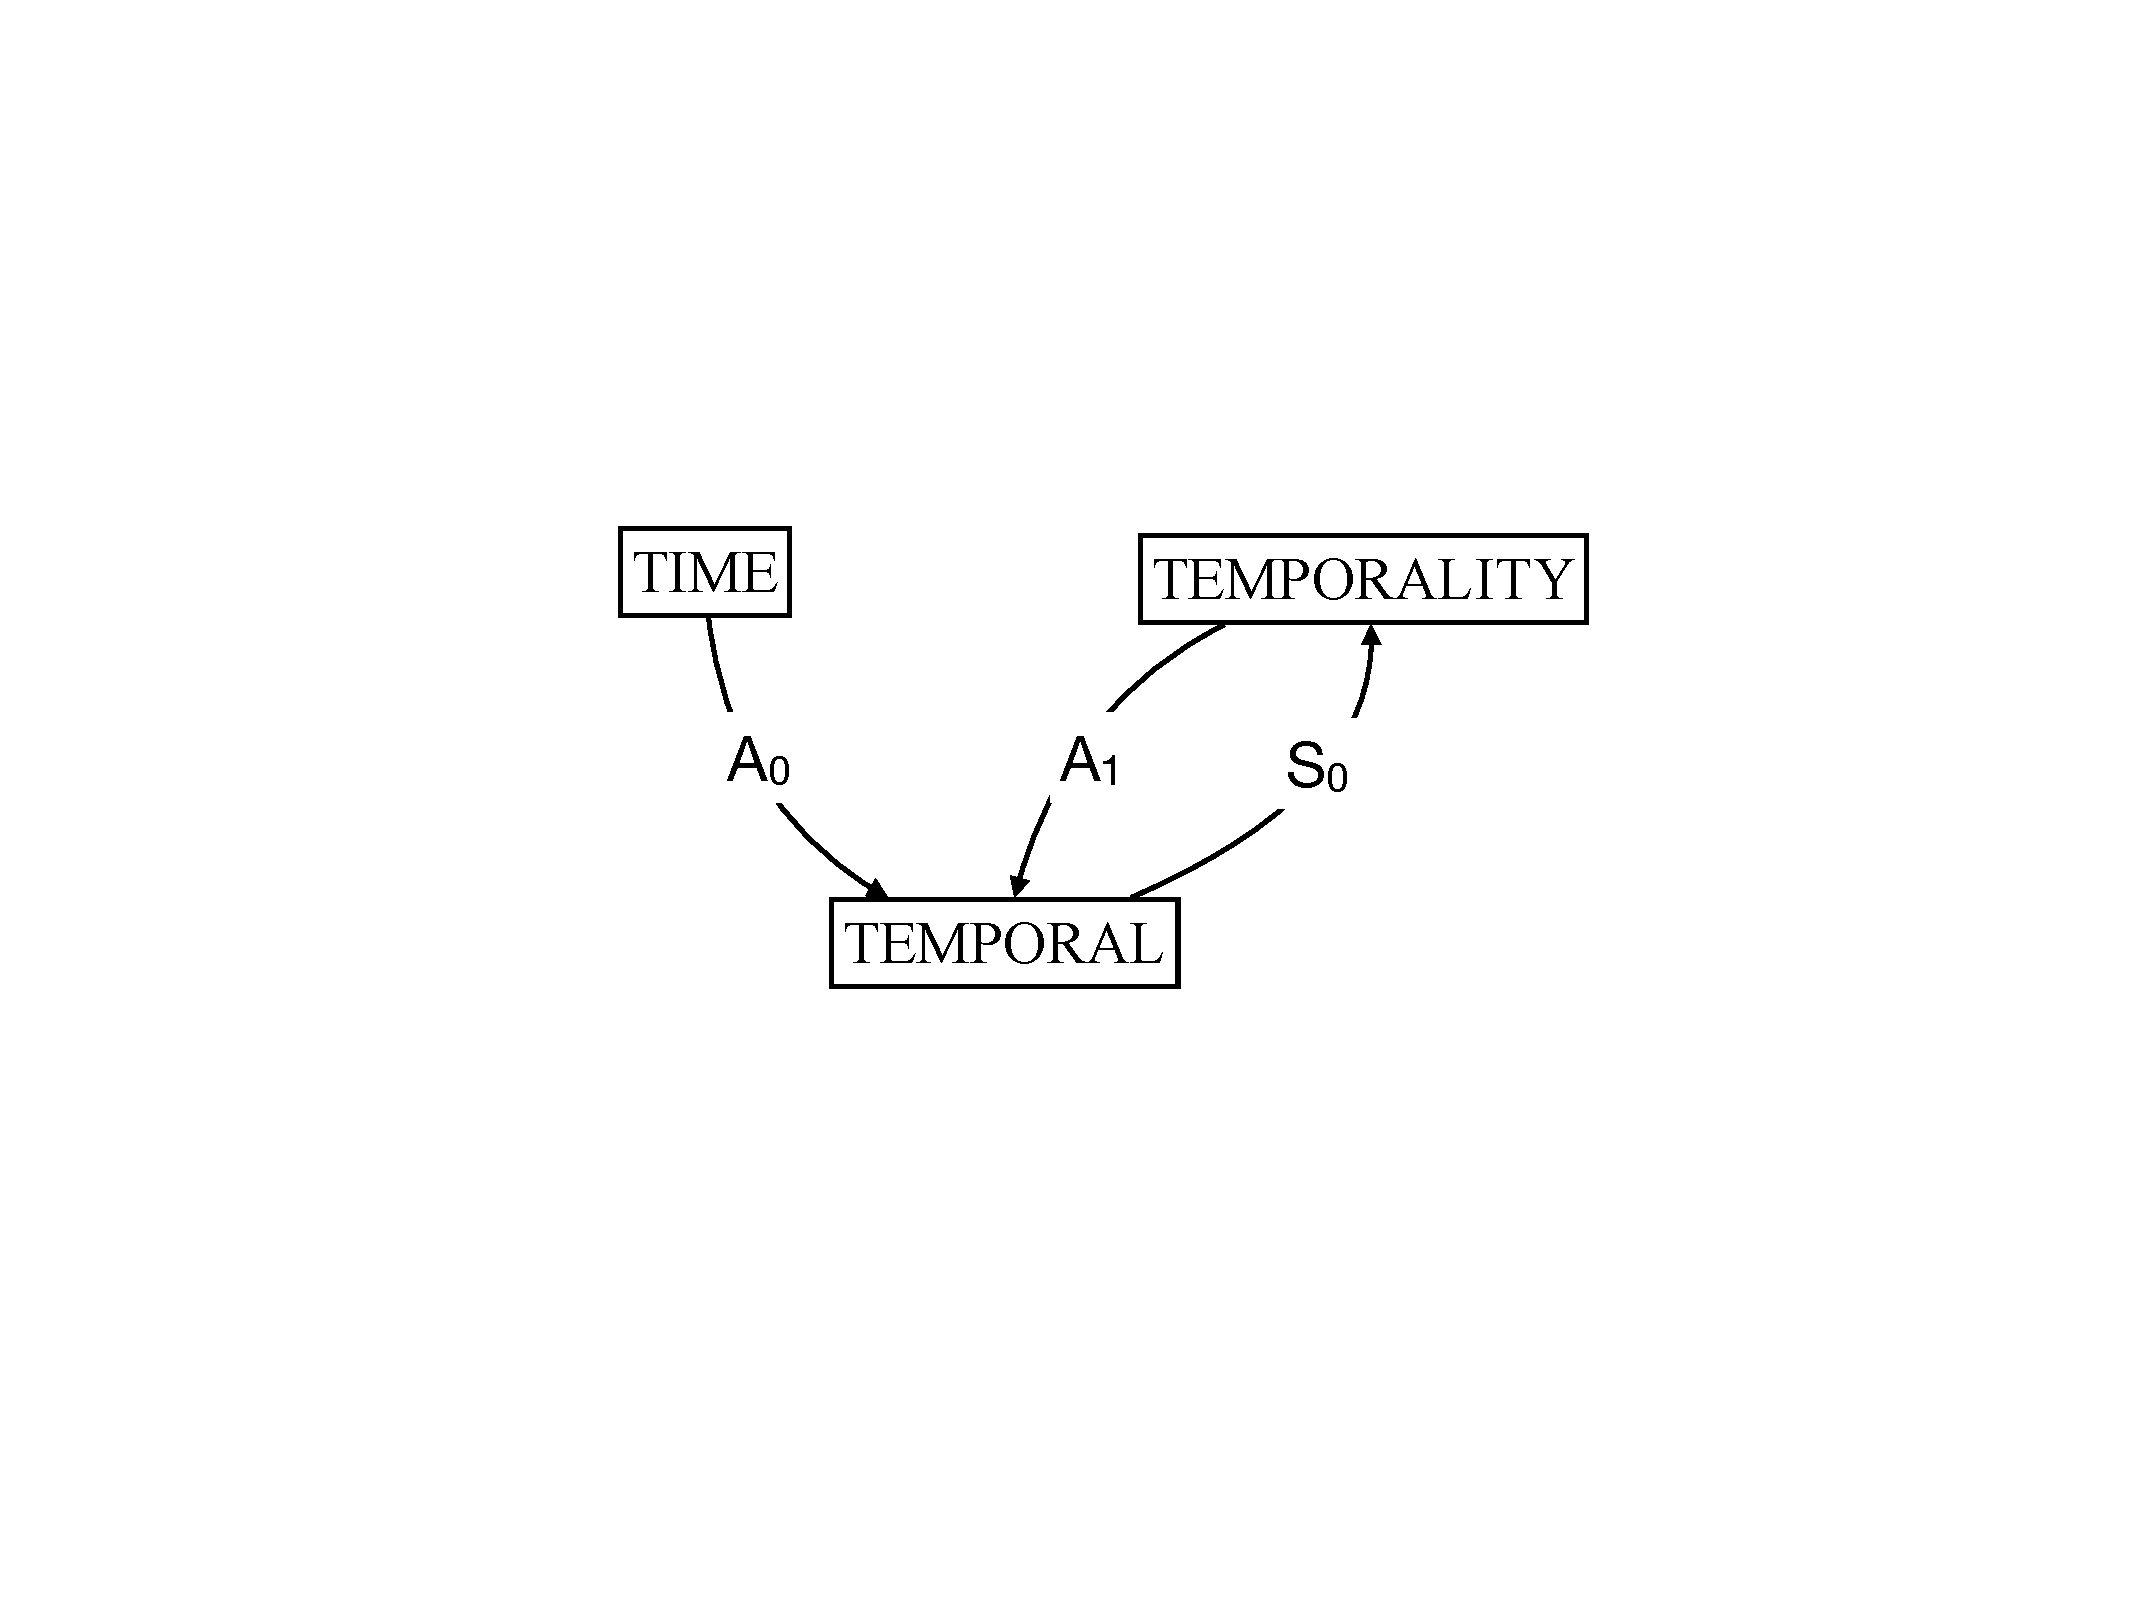
\includegraphics[width=4.7cm]{Fig/ParaLF/configA0S0A1.pdf}
\caption{Typical configuration of lexical links for \lf{A\tsub{0}} $\sim$ \lf{S\tsub{0}} $\sim$  \lf{A\tsub{1}}}\label{fig:configA0S0A1}
\end{figure}

\refstepcounter{LFlist}
\subsubsection*{{\small [\arabic{LFlist}]} \lf{Adv\tsub{0}} \lfgp{{\scriptsize Latin} \textit{adverbium}}: adverbialization}\label{lf:Adv0}
\addcontentsline{toc}{subsection}{{\footnotesize [\arabic{LFlist}]} \lf{Adv\tsub{0}}: adverbialization}\index[lf]{Adv0@\lf{Adv\tsub{0}}|emph}

\lf{Adv\tsub{0}} applies to a non-adverbial lexical unit L and returns an adverb\index[notion]{adverb} having the same meaning as L.

\begin{quote}
\begingroup
\small
\begin{tabular}{ l c c c c}
   \midrule
   \multicolumn{5}{l}{\lf{Adv\tsub{0}}: adverbial} \\
   \midrule
   \textbf{L} & V & N & Adj & Claus \\
   \midrule
   \textbf{\lfappl{Adv\tsub{0}}{L}} & Adv & Adv & Adv & Adv \\
   \midrule
\end{tabular}
\endgroup
\end{quote}

\begin{longtable*}[l]{ l l >{\raggedright\arraybackslash}p{7cm} }

\multicolumn{3}{l}{\textbf{English}} \\*

\lfappl{Adv\tsub{0}}{\textit{see}\tsub{(V)}} & = & \textit{visually} \lfgp{\textit{horrible to see}\enskip$\equiv$\enskip\textit{visually horrible}}  \\
\lfappl{Adv\tsub{0}}{\textit{vision}} & = & \textit{visually}  \\
\lfappl{Adv\tsub{0}}{\textit{alphabet}} & = & \textit{alphabetically}  \\
\lfappl{Adv\tsub{0}}{\textit{rapid}\tsub{(Adj)}} & = & \textit{rapidly}  \\*
\lfappl{Adv\tsub{0}}{\textit{close}\tsub{(Adj)}} & = & \textit{closely}\vspace{6pt}  \\

\multicolumn{3}{l}{\textbf{French}} \\*

\lfappl{Adv\tsub{0}}{\textit{voir}} &= & \textit{visuellement} \lfgp{\textit{insupportable à voir}\enskip$\equiv$\enskip\textit{visuellement insupportable}} \\
\lfappl{Adv\tsub{0}}{\textit{vue}} &= & \textit{visuellement} \\
\lfappl{Adv\tsub{0}}{\textit{alphabet}} &= & \textit{alphabétiquement} \\
\lfappl{Adv\tsub{0}}{\textit{rapide}\tsub{(Adj)}} &= & \textit{rapidement} \\
\lfappl{Adv\tsub{0}}{\textit{proche}} &= & \textit{près}\vspace{6pt} \\

\multicolumn{3}{l}{\textbf{Russian}} \\*

\lfappl{Adv\tsub{0}}{\textit{videt\palati}} & = & \idiom{\textit{na vid}} \lfgp{\textit{protivno videt}\enskip$\equiv$\enskip\textit{protivnyj \idiom{na vid}}} \\
\lfappl{Adv\tsub{0}}{\textit{zrenie}} & = & \textit{zritel\palati{}no} \\
\lfappl{Adv\tsub{0}}{\textit{alfavit}} & = & \textit{po alfavitu} \\
\lfappl{Adv\tsub{0}}{\textit{bystryj}} & = & \textit{bystro} \\*
\lfappl{Adv\tsub{0}}{\textit{blizkij}} & = & \textit{blizko} \\

\end{longtable*}

\lf{Adv\tsub{0}} should not be mistaken for another adverbialization LF, namely \lf{Adv\tsub{i}}\index[lf]{Advi@\lf{Adv\tsub{i}}}, which is examined below (\sectref{sec:derivAdvAct}, [\ref{lf:Adv-i}], p.\thinspace\pageref{lf:Adv-i}):

\begingroup
\small

\ex. \begingroup\setlength{\tabcolsep}{2pt}
\begin{tabular}[t]{ l l l >{\raggedright\arraybackslash}p{7cm} }
{\smaller English} & \lfappl{Adv\tsub{1}}{\textit{see} \lfgp{N\tsub{Y}}} &= & \textit{at the sight} \lfgp{\textit{of} N\tsub{Y}}\quad ($\equiv$\enskip\textit{seeing} \lfgp{N\tsub{Y}})  \\
{\smaller French} & \lfappl{Adv\tsub{1}}{\textit{voir} \lfgp{N\tsub{Y}}} &= & \textit{à la vue} \lfgp{\textit{de} N\tsub{Y}}  \\
{\smaller Russian} & \lfappl{Adv\tsub{1}}{\textit{videt\palati} \lfgp{N\tsub{Y-\textsc{acc}}}} &= & \textit{pri vide} \lfgp{N\tsub{Y-\textsc{gen}}}  \\
\end{tabular}\endgroup

\endgroup

\refstepcounter{LFlist}
\subsubsection*{{\small [\arabic{LFlist}]} \lf{Claus\tsub{0}} \lfgp{{\scriptsize Latin} *\textit{clausativum}}: clausativization}\label{lf:Claus0}
\addcontentsline{toc}{subsection}{{\footnotesize [\arabic{LFlist}]} \lf{Claus\tsub{0}}: clausativization}\index[lf]{Claus0@\lf{Claus\tsub{0}}|emph}

\lf{Claus\tsub{0}} applies to a non-clausative\index[notion]{clausative} lexical unit L and returns a clausative having the same meaning as L.

\lfappl{Claus\tsub{0}}{L} is a clausative lexical entity -- that is, a lexical entity syntactically equivalent to a sentence (cf. \chapref{chap:NotionLF}, \sectref{sec:notionPdD}, p.\thinspace\pageref{txt:Claus0}). \lf{Claus\tsub{0}} turns the meaning of its lexical argument L into the meaning of an utterance communicatively dominated\index[notion]{communicative!\tld\ dominance} by the semantic component `I signal \lfgp{that L ...}'. In this respect, \lf{Claus\tsub{0}} is not a pure structural derivation, just like \lf{A\tsub{0}}\index[lf]{A0@\lf{A\tsub{0}}} (see above, p.\thinspace\pageref{txt:A0NonPurelyStructural}); it adds a piece of communicative information (`I signal \lfgp{that L ...}') to the derivative.

\begin{soundbox}{To signal vs. to communicate}
\index[notion]{signal, to}\notion{To signal} is a term \parencite[249--250]{Melcuk2001b}: in contrast to \notion{to communicate}, it denotes an enunciation mode that precludes negation and interrogation. A signaled expression does not state something about the world, but manifests an internal (mental, emotional or physiological) state of the Speaker.
\end{soundbox}

\begin{quote}
\begingroup
\small
\begin{tabular}{l c c c c }
   \midrule
   \multicolumn{5}{l}{\lf{Claus\tsub{0}}: clausative} \\
   \midrule
   \textbf{L} & V & N & Adj & Adv \\
   \midrule
   \textbf{\lfappl{Claus\tsub{0}}{L}} & Claus & Claus & Claus & Claus \\
   \midrule
\end{tabular}
\endgroup
\end{quote}

\lf{Claus\tsub{0}} should not be mistaken for the \lf{Imper}\index[lf]{Imper@\lf{Imper}} LF (\sectref{sec:flFlexion}, [\ref{lf:Imper}], p.\thinspace\pageref{lf:Imper}), whose values are syntactically also clausatives, but which carry an additional meaning: `I signal that \emph{I want you to do} [L]'. 

\begin{longtable*}[l]{ l l >{\raggedright\arraybackslash}p{7cm} }

\multicolumn{3}{l}{\textbf{English}} \\*

\lfappl{Claus\tsub{0}}{\textit{congratulations}} & = & \textit{Congratulations!}\textbf{,} \textit{Congrats!} \\
\lfappl{Claus\tsub{0}}{\textit{meow}\tsub{(V)}} & = & \textit{Meow!} \\
\lfappl{Claus\tsub{0}Son}{\textit{cat}} & = & \textit{Meow!} \vspace{2pt}\\*
\multicolumn{3}{ p{11cm} }{\leftskip=0.5cm{\small\remark{Note.}For the LF \lf{Son}, see \chapref{chap:syntLFs}, [\ref{lf:Son}], p.\thinspace\pageref{lf:Son}.}} \vspace{2pt}\\
%\lfappl{Claus\tsub{0}Son}{\textit{chute}} & = & \textit{Badaboum !} \\
\lfappl{Claus\tsub{0}}{\textit{explosion}} & = & \textit{Boom!} \\
\lfappl{Claus\tsub{0}}{\textit{gunshot}} & = & \textit{Bang!}\textbf{,} \textit{Pow!} \\
\lfappl{Claus\tsub{0}}{\uslabel{informal} \textit{yucky}} & = & \textit{Yuck!}\vspace{6pt} \\

\multicolumn{3}{l}{\textbf{French}} \\*

\lfappl{Claus\tsub{0}}{\textit{féliciter}} & = & (\textit{Mes}) \textit{Félicitations !}\textbf{;} \textit{Chapeau !} \\
\lfappl{Claus\tsub{0}}{\textit{miauler}} & = & \textit{Miaou !} \\
\lfappl{Claus\tsub{0}Son}{\textit{chat}} & = & \textit{Miaou !} \\
\lfappl{Claus\tsub{0}Son}{\textit{chute}} & = & \textit{Badaboum !} \\
\lfappl{Claus\tsub{0}}{\textit{explosion}} & = & \textit{Boum !} \\
\lfappl{Claus\tsub{0}}{\idiom{\textit{coup de feu}}} & = & \textit{Pan !} \\
\lfappl{Claus\tsub{0}}{\textit{dégoûtant}} & = & \textit{Beurk !}\vspace{6pt} \\

\multicolumn{3}{l}{\textbf{Russian}} \\*

\lfappl{Claus\tsub{0}}{\textit{pozdravlenije}} & = & \textit{Pozdravljaju!} \\
\lfappl{Claus\tsub{0}}{\textit{mjaukat\palati}} & = & \textit{Mjau!} \\
\lfappl{Claus\tsub{0}Son}{\textit{ko\v{s}ka}} & = & \textit{Mjau!} \\
\lfappl{Claus\tsub{0}Son}{\textit{padenie}} & = & \textit{Bax!} \\
\lfappl{Claus\tsub{0}}{\textit{vystrel}} & = & \uslabel{child language} \textit{Pif-paf!} \\
\lfappl{Claus\tsub{0}}{\textit{protivnyj}} & = & \textit{Fi!}\textbf{;} \textit{Fu!} \\

\end{longtable*}

\begin{historicalremark}
The \lf{Claus\tsub{0}} LF was introduced in \textcite{MelcukPolguere2021} in order to better dovetail the set of structural derivative LFs with that of deep parts of speech\index[notion]{part of speech [PoS]!deep \tld}. \lf{Claus\tsub{0}} cancels the neological LF \lf{Enun}\index[lf]{Enun@\lf{Enun} \lfgp{no longer used}} ({\smaller Latin} \textit{\={e}nunti\={a}tus}), which was used in the \notion{DiCo}\index[notion]{lexical database!DiCo}\index[notion]{DiCo} lexicographic\index[notion]{lexicography} project\index[notion]{lexicography} \parencite{Polguere2000b}.
\end{historicalremark}

\section{Predicative derivatives}\label{sec:derivationPredicativisation}

\refstepcounter{LFlist}
\subsubsection*{{\small [\arabic{LFlist}]} \lf{Pred} \lfgp{{\scriptsize Latin} *\textit{praedic\={a}tum} `[a] predicate'}: predicativization}\label{lf:Pred}
\addcontentsline{toc}{subsection}{{\footnotesize [\arabic{LFlist}]} \lf{Pred}: predicativization}\index[lf]{Pred@\lf{Pred}|emph}

\lfappl{Pred}{L} is a verbal lexical unit that means `be\tsub{(copul)}~L'; it serves to turn a predicative\index[notion]{predicativity} noun, an adjective or an adverb L into a verb. Thus, \lf{Pred} plays the role of the copula\index[notion]{copula verb}\index[notion]{verb!copula \tld}; it is the paradigmatic counterpart of the syntagmatic LF \lf{Copul}\index[notion]{lexical function!paradigmatic vs. syntagmatic \tlds} (\chapref{chap:syntLFs}, [\ref{lf:Copul}], p.\thinspace\pageref{lf:Copul}).

Note that for adjectives and adverbs, the LF \lf{Pred} is semantically equivalent to \lf{V\tsub{0}}\index[lf]{V0@\lf{V\tsub{0}}} (see above, [\ref{lf:V0}], p.\thinspace\pageref{lf:V0}):

\begingroup
\small

\ex. \lfappl{Pred}{\textit{unexpected}}\thinspace=\thinspace\lfappl{V\tsub{0}}{\textit{unexpected}} \thinspace=\thinspace \idiom{\textit{come as a bolt from the blue}}

\endgroup

For quasi-predicative\index[notion]{predicate, semantic!quasi-\tld}\index[notion]{quasi-predicate} nouns denoting Agents\index[notion]{Agent (semantic role)!\tld\ noun}, \lf{Pred} is semantically equivalent to \lf{Fact\tsub{0}}\index[lf]{Facti@\lf{Fact\tsub{i}}!\lf{Fact\tsub{0}}} (\chapref{chap:syntLFs}, [\ref{lf:Fact-i}], p.\thinspace\pageref{txt:Fact0Descr}):

\begingroup
\small

\ex. \lfappl{Pred}{\textit{cook}\tsub{(N)}}\thinspace=\thinspace\lfappl{Fact\tsub{0}}{\textit{cook}\tsub{(N)}} \thinspace=\thinspace \textit{cook}\tsub{(V)} {\small `be a cook'}

\endgroup

\begin{quote}
\begingroup
\small
\begin{tabular}{ l c c c }
   \midrule
   \multicolumn{4}{l}{\lf{Pred}: verbal} \\
   \midrule
   \textbf{L} & N\tsub{(predic)} & Adj & Adv \\
   \midrule
   \textbf{\lfappl{Pred}{L}} & V & V & V \\
   \midrule
\end{tabular}
\endgroup
\end{quote}

\begin{longtable*}[l]{ l l >{\raggedright\arraybackslash}p{7cm} }

\multicolumn{3}{l}{\textbf{English}} \\*

\lfappl{Pred}{\textit{beggar}} & = & \textit{beg} {\small `be a beggar'} \lfgp{\textit{He begs for a living.}} \\
\lfappl{Pred}{\textit{cook}\tsub{(N)}} & = & \textit{cook}\tsub{(V)} {\small `be a cook'} \lfgp{\textit{He cooks in a posh restaurant.}} \\
\lfappl{Pred}{\textit{unexpected}} & = & \idiom{\textit{come as a bolt from the blue}} \\
\lfappl{Pred}{\textit{inseparable}} & = & \idiom{\textit{be joined at the hip}} \vspace{6pt} \\

\multicolumn{3}{l}{\textbf{French}} \\*

\lfappl{Pred}{\textit{mendiant}} & = & \textit{mendier} \\
\lfappl{Pred}{\textit{cuisinier}} & = & \textit{cuisiner} \\
\lfappl{Pred}{\textit{aisé} \lfgp{financièrement}} &= & \idiom{\textit{avoir les moyens}} \\
\lfappl{Pred\tsub{$\supset$}}{\textit{riche}\tsub{(Adj)}} &= & \uslabel{colloquial} \idiom{\textit{péter dans la soie}} \\
\lfappl{Pred}{\textit{inséparables}\tsub{(Adj)}} & = & \idiom{\textit{être comme les} (\textit{cinq}) \textit{doigts de la main}}\textbf{,} \\
 & & \idiom{\textit{être comme les deux doigts de la main}} \vspace{6pt} \\

\multicolumn{3}{l}{\textbf{Russian}} \\*

\lfappl{Pred}{\textit{ni\v{s}\v{c}ij}} & = & \textit{ni\v{s}\v{c}enstvovat\palati} \\
\lfappl{Pred}{\textit{direktor}} & = & \textit{direktorstvovat\palati} \\
\lfappl{Pred\tsub{$\supset$}}{\textit{bogatyj}} &= & \idiom{\textit{katat\palati{}sja kak syr v masle}} \\
\lfappl{Pred}{\textit{neo\v{z}idannyj}} & = & \uslabel{literary} \idiom{\textit{pojavit\palati{}sja kak \v{c}ërt iz tabakerki}} \\
\lfappl{Pred}{\textit{nerazlu\v{c}ny}} & = & \uslabel{colloquial} \idiom{\lfgp{N\tsub{X-\textsc{acc}}} \textit{vodoj ne razol\palati{}ë\v{s}\palati}} \\

\end{longtable*}

\paragraph*{\lf{Pred} in configurational\slashs complex LFs.}\index[notion]{lexical function!complex \tld}\index[notion]{lexical function!configurational \tld}\index[notion]{complex LF}\index[notion]{configurational LF}

\lf{Pred} is mostly combined with adjectival\slashs{}adverbial LFs \lf{Magn}\index[lf]{Magn@\lf{Magn}}, \lf{Ver}\index[lf]{Ver@\lf{Ver}} and \lf{Bon}\index[lf]{Bon@\lf{Bon}} (\chapref{chap:syntLFs}, \sectref{sec:collocatifsModif}, [\ref{lf:Magn}\slashs\ref{lf:Ver}\slashs\ref{lf:Bon}], p.\thinspace\pageref{lf:Magn}) to form configurational or complex LFs.

\begingroup
\small

\ex. \begingroup\setlength{\tabcolsep}{2pt}
\begin{tabular}[t]{ l l l >{\raggedright\arraybackslash}p{4.5cm} }
{\smaller English} & \lfappl{Magn+Pred}{\textit{angry}} & = & \textit{fume}\tsub{(V)} \\
{\smaller English} & \lfappl{Magn+Pred}{\textit{hungry}} & = & \textit{starve} \\
{\smaller French} & \lfappl{Magn+Pred}{\textit{chauve}\tsub{(N)} {\small `bald person'}} & = & \uslabel{vulgar} $\ulcorner$\textit{\begin{otherlanguage}{french}avoir une perruque en peau de fesse\end{otherlanguage}}$\urcorner$ {\footnotesize lit. `have a buttock-skin wig'} \\
{\smaller English} & \lfappl{PredMagn}{\textit{animosity}} = & & \\
 & \lfappl{Magn+Func\tsub{0}}{\textit{animosity}} & = & \idiom{\textit{run rampant}} \\
{\smaller English} & \lfappl{PredVer}{\textit{dress}\tsub{(N)}} & = & \textit{fit}\tsub{(V)}\textbf{;} \idiom{\textit{sit well}} \lfgp{\textit{with} N} \\
%\textrm{French} & \lfappl{Bon+Pred}{\textit{temps} {\scriptsize `weather'}} & = & \idiom{\textit{faire beau}} \\
\end{tabular}\endgroup

\endgroup

Note that cases of the configurational \emph{paradigmatic}\index[notion]{lexical function!paradigmatic vs. syntagmatic \tlds} LF \lf{Magn+Pred} were mistakenly described as cases of the complex \emph{syntagmatic} LF \lf{PredMagn} in \textcite[216--217]{Melcuk2015a-e}.

For more on the use of \lf{Pred} in complex LFs, see the description of the syntagmatic LF \lf{Plus}\index[lf]{Plus@\lf{Plus}} (\chapref{chap:syntLFs}, [\ref{lf:Plus}], p.\thinspace\pageref{lf:Plus}).

\section{Nominal derivatives}\label{sec:derivNom}

Nominal derivatives fall into two classes: actantial (\sectref{sec:derivNomAct}) vs. circumstantial (\sectref{sec:derivNomCirc}). Note that adjectival (\sectref{sec:derivAdjAct}) and adverbial (\sectref{sec:derivAdvAct}) derivatives are only actantial.

\subsection{Nominal actantial derivatives}\label{sec:derivNomAct}

This section presents, in the first place, the LFs \lf{S\tsub{1}}, \lf{S\tsub{2}}, \lf{S\tsub{3}}, ... -- for short, \lf{S\tsub{i}}. \lf{S\tsub{i}} applies to a predicative lexical unit\index[notion]{predicativity} -- predicate\index[notion]{predicate, semantic} or quasi-predicate\index[notion]{predicate, semantic!quasi-\tld} -- and returns the name for its DSyntA\thinspace\syntDname{I}, \syntDname{II}, \syntDname{III}, ...

Also included in this section are two more specific LFs intimately related to \lf{S\tsub{i}}: \lf{Equip} and \lf{Cap}.

\refstepcounter{LFlist}
\subsubsection*{{\small [\arabic{LFlist}]} \lf{S\tsub{i}}: typical name for L's DSyntA\thinspace\syntDname{i}}\label{lf:S-i}
\addcontentsline{toc}{subsection}{{\footnotesize [\arabic{LFlist}]} \lf{S\tsub{i}}: typical name for L's DSyntA\thinspace\syntDname{i}}\index[lf]{Si@\lf{S\tsub{i}}|emph}

\lfappl{S\tsub{i}}{L} is a nominal lexical entity that is the name for L's DSyntA\thinspace\syntDname{I}, \syntDname{II}, \syntDname{III}, ...

\begin{quote}
\begingroup
\small
\begin{tabular}{ l  c c c c c }
   \midrule
   \multicolumn{6}{l}{\lf{S\tsub{i}}: nominal} \\
   \midrule
   \textbf{L} & V & N & Adj & Adv & Claus \\
   \midrule
   \textbf{\lfappl{S\tsub{i}}{L}} & N & N & N & N & N\\
   \midrule
\end{tabular}
\endgroup
\end{quote}

\begin{longtable*}[l]{ l l >{\raggedright\arraybackslash}p{7cm} }

\multicolumn{3}{l}{\textbf{English}} \\*

\lfappl{S\tsub{1}}{\textit{sell}\tsub{(V)}} & = & \textit{seller} \\
\multicolumn{3}{l}{\quad\lfgp{N\tsub{X} \textit{sells} N\tsub{Y} \textit{to} N\tsub{Z} \textit{for} N\tsub{W}}} \\
\lfappl{S\tsub{2}}{\textit{sell}\tsub{(V)}} & = & \textit{merchandise} \\
\lfappl{S\tsub{3}}{\textit{sell}\tsub{(V)}} & = & \textit{buyer} \\
\lfappl{S\tsub{4}}{\textit{sell}\tsub{(V)}} & = & \textit{price} \\
\lfappl{S\tsub{1}}{\textit{chemistry}} & = & \textit{chemist} \\
\multicolumn{3}{l}{\quad\lfgp{\textit{chemistry done by} N\tsub{X}}} \\
\lfappl{S\tsub{1}}{\textit{mute}\tsub{(Adj)}} & = & \textit{mute}\tsub{(N)} \\
\multicolumn{3}{l}{\quad\lfgp{N\tsub{X} \textit{is mute}}} \\
\lfappl{S\tsub{1}}{\textit{lazy}} & = & \uslabel{colloquial} \textit{lazybones} \\
\multicolumn{3}{l}{\quad\lfgp{N\tsub{X} \textit{is lazy}}}\vspace{6pt} \\

\multicolumn{3}{l}{\textbf{French}} \\*

\lfappl{S\tsub{1}}{\textit{vendre}} & = & \textit{vendeur} \\
\lfappl{S\tsub{2}}{\textit{vendre}} & = & \textit{marchandise} \\
\lfappl{S\tsub{3}}{\textit{vendre}} & = & \textit{acheteur} \\
\lfappl{S\tsub{4}}{\textit{vendre}} & = & \textit{prix} \\
\lfappl{S\tsub{1}}{\textit{chimie}} & = & \textit{chimiste} \\
\lfappl{S\tsub{1}}{\textit{muet}\tsub{(Adj)}} & = & \textit{muet}\tsub{(N)}\vspace{6pt} \\
%\lfappl{S\tsub{2}}{\textit{À bas} \lfgp{N\tsub{Y}} \textit{!}} & = & \textit{ennemi} \\

\multicolumn{3}{l}{\textbf{Russian}} \\*

\lfappl{S\tsub{1}}{\textit{prodavat\palati}} & = & \textit{prodavec} \\
\lfappl{S\tsub{2}}{\textit{prodavat\palati}} & = & \textit{tovar} \\
\lfappl{S\tsub{3}}{\textit{prodavat\palati}} & = & \textit{pokupatel\palati} \\
\lfappl{S\tsub{4}}{\textit{prodavat\palati}} & = & \textit{cena} \\
\lfappl{S\tsub{1}}{\textit{ximija}} & = & \textit{ximik} \\
\lfappl{S\tsub{1}}{\textit{nemoj}\tsub{(Adj)}} & = & \textit{\textit{nemoj}}\tsub{(N)} \\

\end{longtable*}

\refstepcounter{LFlist}
\subsubsection*{{\small [\arabic{LFlist}]} \lf{Equip} \lfgp{{\scriptsize French} \textit{équipage} `crew'}: team that allows L's referent\index[notion]{referent} to function}\label{lf:Equip}
\addcontentsline{toc}{subsection}{{\footnotesize [\arabic{LFlist}]} \lf{Equip}: team that allows L's referent to function}\index[lf]{Equip@\lf{Equip}|emph}

\lfappl{Equip}{L} is a nominal lexical entity that designates an organized set of individuals (or, more generally, of living beings) involved in the functioning of L's referent; in other words, \lfappl{Equip}{L} designates the set of L's DSyntAs~\syntDname{I}. Consequently, L is a quasi-predicative\index[notion]{predicate, semantic!quasi-\tld}\index[notion]{quasi-predicate} noun denoting a functioning entity\index[notion]{entity@`entity'}.

\begin{quote}
\begingroup
\small
\begin{tabular}{ l c }
   \midrule
   \multicolumn{2}{l}{\lf{Equip}: nominal} \\
   \midrule
   \textbf{L} & N  \\
   \midrule
   \textbf{\lfappl{Equip}{L}} & N \\
   \midrule
\end{tabular}
\endgroup
\end{quote}

\begin{longtable*}[l]{ l l >{\raggedright\arraybackslash}p{7cm} }

\multicolumn{3}{l}{\textbf{English}} \\*

\lfappl{Equip}{\textit{ship}\tsub{(N)}} & = & \textit{crew} \\
\lfappl{Equip}{\textit{theater}} & = & \textit{company} \\
\lfappl{Equip}{\textit{newspaper}} & = & \idiom{\textit{editorial staff}}\vspace{6pt} \\

\multicolumn{3}{l}{\textbf{French}} \\*

\lfappl{Equip}{\textit{navire}} & = & \textit{équipage} \\
\lfappl{Equip}{\textit{théâtre}} & = & \textit{troupe} \\
\lfappl{Equip}{\textit{journal}} & = & \textit{rédaction}\vspace{6pt} \\

\multicolumn{3}{l}{\textbf{Russian}} \\*

\lfappl{Equip}{\textit{sudno}} & = & \textit{èkipa\v{z}} \\
\lfappl{Equip}{\textit{teatr}} & = & \textit{truppa} \\
\lfappl{Equip}{\textit{gazeta}} & = & \textit{redakcija} \\

\end{longtable*}

\newpage
According to its nature, \lf{Equip} applies only to lexical units whose DSyntA\thinspace\syntDname{I} denotes a participant -- \lfappl{S\tsub{1}}{L} -- that makes the entity L function.  In other words, \lf{Equip} means `set of \lf{S\tsub{1}}'; compare the above English illustrations of \lf{Equip} with~\Next:

\begingroup
\small

\ex. \begingroup\setlength{\tabcolsep}{2pt}
\begin{tabular}[t]{ l l >{\raggedright\arraybackslash}p{7cm} }
\lfappl{S\tsub{1}}{\textit{ship}\tsub{(N)}} & = & \textit{sailor} \lfgp{(\textit{ship's}) \textit{crew}\enskip$\equiv$\enskip\textit{set of sailors}} \\
\lfappl{S\tsub{1}}{\textit{theater}} & = & \textit{actor} \lfgp{(\textit{theater's}) \textit{company}\enskip$\equiv$\enskip\textit{set of actors}} \\
\lfappl{S\tsub{1}}{\textit{newspaper}} & = & \textit{journalist} \lfgp{\idiom{\textit{editorial staff}}\enskip$\equiv$\enskip\textit{set of journalists}} \\
\end{tabular}\endgroup

\endgroup

The meaning `set [of Xs]' is represented by the LF \lf{Mult}\index[lf]{Mult@\lf{Mult}} (\sectref{sec:flFlexion}, [\ref{lf:Mult}], p.\thinspace\pageref{lf:Mult}). It is thus possible to propose a paraphrasing rule \textbf{R\tsub{\lf{Equip}}} that states the following semantic equivalence:

\begin{center}
\phantomsection\label{txt:RParaphEquip}\APolbox{8.5cm}{%
\renewcommand{\arraystretch}{1.1}
\begin{tabular}{ l l }
\textbf{R\tsub{\lf{Equip}}:} & \lfappl{Equip}{L}\enskip{\small$\equiv$}\enskip\lfappl{MultS\tsub{1}}{L} \\*
& {\small\textit{crew} \senseex{of a ship}\enskip$\equiv$\enskip\textit{set of sailors}\tsub{\lfappl{S$_\text{1}$}{\textit{ship}}} \senseex{of a ship}} \\
\end{tabular}
}
\end{center}\index[notion]{paraphrase!deep-syntactic paraphrasing rule!\textbf{R\tsub{\lf{Equip}}}|emph}

We can foresee a possible generalization of the LF \lf{Equip} in order to cover cases corresponding to \lf{MultS\tsub{2}}, \lf{MultS\tsub{3}}, etc. With such a generalization, it would be necessary to distinguish \lf{Equip\tsub{1}}, \lf{Equip\tsub{2}}, \lf{Equip\tsub{3}}, etc.

\refstepcounter{LFlist}
\subsubsection*{{\small [\arabic{LFlist}]} \lf{Cap} \lfgp{{\scriptsize Latin} \textit{caput} `head'}: person in charge of L's referent\index[notion]{referent}}\label{lf:Cap}
\addcontentsline{toc}{subsection}{{\footnotesize [\arabic{LFlist}]} \lf{Cap}: person in charge of L's referent}\index[lf]{Cap@\lf{Cap}|emph}

\lfappl{Cap}{L} is a nominal lexical entity that designates the individual in charge of a functioning entity L (in fact, in charge of the set of L's DSyntAs\thinspace\syntDname{I}). As for \lf{Equip}, L is a quasi-predicative\index[notion]{predicate, semantic!quasi-\tld}\index[notion]{quasi-predicate} noun.

\begin{quote}
\begingroup
\small
\begin{tabular}{ l c }
   \midrule
   \multicolumn{2}{l}{\lf{Cap}: nominal} \\
   \midrule
   \textbf{L} & N  \\
   \midrule
   \textbf{\lfappl{Cap}{L}} & N \\
   \midrule
\end{tabular}
\endgroup
\end{quote}

\lfappl{Cap}{L} denotes a specific element of the set of \lfappl{S\tsub{1}}{L}. Two cases have to be distinguished:

\begin{itemize}

\item if L denotes a group of individuals (e.g. a tribe, a pack of animals, etc.), \lfappl{Cap}{L} denotes the main member of this group;

\item if L denotes a functioning entity (e.g. a plane, a school, etc.) run by a group of individuals -- that is, run by \lfappl{Equip}{L}\index[lf]{Equip@\lf{Equip}}, \lfappl{Cap}{L} is the main member of \lfappl{Equip}{L}.

\end{itemize}

\begin{longtable*}[l]{ l l >{\raggedright\arraybackslash}p{7cm} }

\multicolumn{3}{l}{\textbf{English}} \\*

\lfappl{Cap}{\textit{kingdom}} & = & \textit{king} \\
\lfappl{Cap}{\textit{mafia}} & = & \textit{don}\textbf{,} \textit{godfather} \\
\lfappl{Cap}{\textit{ship}\tsub{(N)}} & = & \textit{captain}\sensenum{1} \\
\lfappl{Cap}{\textit{plane}\tsub{(N)}} & = & \textit{captain}\sensenum{2} \\
\lfappl{Cap}{\textit{school}\tsub{(N)}} & = & \textit{principal}\tsub{(N)} \\
\lfappl{Cap}{\textit{tribe}} & = & \textit{chief} (\textit{of} \textsc{art} \tld) \\
\lfappl{Cap}{\lfgp{\textit{wolf}} \textit{pack}\tsub{(N)}} & = & \textit{leader} (\textit{of} \textsc{art} \tld)\vspace{6pt} \\

\multicolumn{3}{l}{\textbf{French}} \\*

\lfappl{Cap}{\textit{royaume}} & = & \textit{roi} \\
\lfappl{Cap}{\textit{mafia}} & = & \textit{parrain} \\
\lfappl{Cap}{\textit{navire}} & = & \textit{capitaine}\sensenum{1} \\
\lfappl{Cap}{\textit{avion}} & = & \textit{capitaine}\sensenum{2}\textbf{,} \textit{commandant} (\textit{de bord}) \\
\lfappl{Cap}{\textit{gare}} & = & \idiom{\textit{chef de gare}} \\
\lfappl{Cap}{\textit{tribu}} & = & \textit{chef}\sensenum{1} (\textit{de} (\textsc{art}) \tld) \\
\lfappl{Cap}{\textit{meute}} & = & \textit{chef}\sensenum{2} (\textit{de} (\textsc{art}) \tld)\vspace{6pt} \\

\multicolumn{3}{l}{\textbf{Russian}} \\*

\lfappl{Cap}{\textit{korolevstvo}} & = & \textit{korol\palati} \\
\lfappl{Cap}{\textit{mafija}} & = & \textit{boss} \\
\lfappl{Cap}{\textit{sudno}} & = & \textit{kapitan} \\
\lfappl{Cap}{\textit{samolët}} & = & \idiom{\textit{komandir korablja}} \\
\lfappl{Cap}{\textit{plem\suffixsplit ja}} & = & \textit{vo\v{z}d\palati} (\tld\textit{eni}) \\
\lfappl{Cap}{\textit{sta\suffixsplit ja}} & = & \textit{vo\v{z}ak} (\tld\textit{i}) \\

\end{longtable*}

\subsection{Nominal circumstantial derivatives}\label{sec:derivNomCirc}\index[notion]{circumstantial}

As seen above, \lf{S\tsub{i}}\index[lf]{Si@\lf{S\tsub{i}}} applies to a predicative or quasi-predicative\index[notion]{predicate, semantic}\index[notion]{predicate, semantic!quasi-\tld}\index[notion]{quasi-predicate} lexical unit L and returns the general name for DSyntA\thinspace\syntDname{i} of L. In contrast, the next five LFs -- \lf{S\tsub{loc}}\index[lf]{Sloc@\lf{S\tsub{loc}}}, \lf{S\tsub{instr}}\index[lf]{Sinstr@\lf{S\tsub{instr}}}, \lf{S\tsub{med}}\index[lf]{Smed@\lf{S\tsub{med}}}, \lf{S\tsub{res}}\index[lf]{Sres@\lf{S\tsub{res}}} and \lf{S\tsub{mod}}\index[lf]{Smod@\lf{S\tsub{mod}}} -- return for L the name of L's prototypical \notion{circumstantials} (a.k.a. adverbials, or adjuncts): locative, instrumental, means, result and manner circumstantials.

The domain of application\index[notion]{domain of application of an LF}\index[notion]{application of an LF!domain of \tld}\index[notion]{lexical function!domain of application of a \tld} of a circumstantial LF is determined by its semantic content, namely:

\begin{itemize}

\item \lf{S\tsub{loc}} applies to an L that denotes either an entity or a fact (action, event, process, state, ...), since both entities and facts can have localizations;

\item \lf{S\tsub{instr}} and \lf{S\tsub{med}} apply to an L that denotes an action -- i.e. a particular type of fact, since only actions involve instruments and means;

\item \lf{S\tsub{res}} and \lf{S\tsub{mod}} take an L that denotes a dynamic fact (action, event, process): only dynamic facts have results and happen in a certain way.

\end{itemize}

Because of their particular semantic content, the circumstantial LFs do not apply to adjectives and adverbs. All circumstantial LFs have the same PoS table:

\begin{quote}
\begingroup
\phantomsection\label{exLvalPossible}\small
\begin{tabular}{ l c c c }
   \midrule
   \multicolumn{4}{l}{\lf{S\tsub{loc\slashs{}instr\slashs{}med\slashs{}res\slashs{}mod}}: nominal} \\
   \midrule
   \textbf{L} & V & N & Claus \\
   \midrule
   \textbf{\lfappl{S\tsub{loc\slashs{}instr\slashs{}med\slashs{}res\slashs{}mod}}{L}} & N & N & N \\
   \midrule
\end{tabular}
\endgroup
\end{quote}

The order\index[notion]{lexical function!ordering of \tlds}\index[notion]{ordering of LFs} of presentation of circumstantial LFs follows, roughly speaking, the hierarchy of circumstantials in natural languages: from more to less linguistically privileged circumstantials.

\begin{historicalremark}
A different ordering\index[notion]{lexical function!ordering of \tlds}\index[notion]{ordering of LFs} of circumstantial LFs was used in previous publications, namely: \lf{S\tsub{loc}}, instead of heading the enumeration, was arbitrarily placed in the penultimate position.
\end{historicalremark}

\refstepcounter{LFlist}
\subsubsection*{{\small [\arabic{LFlist}]} \lf{S\tsub{loc}} \lfgp{{\scriptsize Latin} \textit{locus} `place'}: name of the prototypical location}\label{lf:S-loc}
\addcontentsline{toc}{subsection}{{\footnotesize [\arabic{LFlist}]} \lf{S\tsub{loc}}: name of the prototypical location}\index[lf]{Sloc@\lf{S\tsub{loc}}|emph}

\lfappl{S\tsub{loc}}{L} is a nominal lexical entity that is the name of the prototypical location of the referent of L.

\begin{longtable*}[l]{ l l >{\raggedright\arraybackslash}p{6cm} }

\multicolumn{3}{l}{\textbf{English}} \\*

\lfappl{S\tsub{loc}}{\textit{surgery}} & = & \idiom{\textit{operation room}} \\
\lfappl{S\tsub{loc}}{\textit{smoke}\tsub{(V)}} & = & \idiom{\textit{smoking area}}\textbf{;} \idiom{\textit{smoking room}} \\
\lfappl{S\tsub{loc}}{\uslabel{formal} \textit{excrete}} & = & \textit{bathroom}\textbf{,} \textit{restroom}\textbf{,} \textit{toilet}\tsub{(N)}\textbf{,} \textit{washroom}\textbf{;} \textit{privy}\textbf{;} \textit{outhouse} \\
\lfappl{S\tsub{loc}}{\textit{orphan}} & = & \textit{orphanage} \\
\lfappl{S\tsub{loc}}{\textit{cattle}} & = & \textit{stable}\tsub{(N)}\vspace{6pt} \\

\multicolumn{3}{l}{\textbf{French}} \\*

\lfappl{S\tsub{loc}}{\textit{opération} \lfgp{chirurgicale}} & = & \idiom{\textit{salle d'opération}}\textbf{;} \idiom{\textit{bloc opératoire}} \\
\lfappl{S\tsub{loc}}{\textit{fumer}} & = & \textit{espace fumeur}(\textit{s})\textbf{;} \textit{fumoir} \\
\lfappl{S\tsub{loc}}{\idiom{\textit{faire ses besoins}}} & = & \uslabel{vulgar} \textit{chiottes}\textbf{,} \textit{toilettes}\textbf{,} \textit{W.-C.}\textbf{;} \uslabel{formal}~\idiom{\textit{lieu d'aisance}(\textit{s})}\textbf{;} \textit{latrine} \\
\lfappl{S\tsub{loc}}{\textit{orphelin}} & = & \textit{orphelinat} \\
\lfappl{S\tsub{loc}}{\textit{bétail}} & = & \textit{étable}\vspace{6pt} \\

\multicolumn{3}{l}{\textbf{Russian}} \\*

\lfappl{S\tsub{loc}}{\textit{operacija}} & = & \textit{operacionnaja} \\
\lfappl{S\tsub{loc}}{\textit{kurit\palati}} & = & \idiom{\textit{mesto dlja kurenija}}\textbf{,} \uslabel{colloquial}~\textit{kurilka} \\
\lfappl{S\tsub{loc}}{\uslabel{colloquial} \idiom{\textit{spravljat\palati nu\v{z}du}}} & = & \textit{tualet}\textbf{,} \textit{ubornaja}\textbf{;} \uslabel{colloquial}~\textit{sortir} \\
\lfappl{S\tsub{loc}}{\textit{sirota}} & = & \idiom{\textit{detskij dom}} \\
\lfappl{S\tsub{loc}}{\textit{skot}} & = & \textit{xlev} \\

\end{longtable*}

\refstepcounter{LFlist}
\subsubsection*{{\small [\arabic{LFlist}]} \lf{S\tsub{instr}} \lfgp{{\scriptsize Latin} \textit{instrumentum} `tool'}: name of the prototypical instrument}\label{lf:S-instr}
\addcontentsline{toc}{subsection}{{\footnotesize [\arabic{LFlist}]} \lf{S\tsub{instr}}: name of the prototypical instrument}\index[lf]{Sinstr@\lf{S\tsub{instr}}|emph}

\lfappl{S\tsub{instr}}{L} is a nominal lexical entity that is the name of the instrument, in the most general sense, which is prototypically used to do L.

\begin{longtable*}[l]{ l l >{\raggedright\arraybackslash}p{7cm} }

\multicolumn{3}{l}{\textbf{English}} \\*

\lfappl{S\tsub{instr}}{\textit{drink}\tsub{(V)}} & = & \textit{glass}\textbf{;} \textit{cup} \\
\lfappl{S\tsub{instr}}{\textit{shower}\tsub{(V)}} & = & \textit{shower}\tsub{(N)}\sensenum{II} \lfgp{equipment} \\
\lfappl{S\tsub{instr}}{\textit{wash}\tsub{(V)} \lfgp{oneself}} & = & \textit{washcloth} \\
\lfappl{S\tsub{instr}}{\textit{fry}\tsub{(V)}} & = & \idiom{\textit{frying pan}}\textbf{,} \textit{skillet}\textbf{;} \textit{fryer} \\
\lfappl{S\tsub{instr}}{\textit{smell}\tsub{(V)}} & = & \textit{nose}\tsub{(N)} \\
\lfappl{S\tsub{instr}}{\textit{murder}\tsub{(N)}} & = & \idiom{\textit{murder weapon}} \\
\lfappl{S\tsub{instr}}{\textit{Snip!}} & = & \textit{scissors}\vspace{6pt} \\

\multicolumn{3}{l}{\textbf{French}} \\*

\lfappl{S\tsub{instr}}{\textit{boire}} & = & \textit{verre}\textbf{;} \textit{tasse} \\
\lfappl{S\tsub{instr}}{\textit{se doucher}} & = & \textit{douche}\sensenum{II} \lfgp{equipment} \\
\lfappl{S\tsub{instr}}{\textit{se laver}} & = & \idiom{\textit{gant de toilette}} \\
\lfappl{S\tsub{instr}}{\textit{frire}} & = & \senseex{une} \textit{poêle}\textbf{;} \textit{friteuse} \\
\lfappl{S\tsub{instr}}{\textit{sentir}} & = & \textit{nez} \\
\lfappl{S\tsub{instr}}{\textit{crime}} & = & \idiom{\textit{arme du crime}} \\
\lfappl{S\tsub{instr}}{\textit{Glouglou !} } & = & \textit{verre}\vspace{6pt} \\

\multicolumn{3}{l}{\textbf{Russian}} \\*

\lfappl{S\tsub{instr}}{\textit{pit\palati}} & = & \textit{stakan}\textbf{;} \textit{\v{c}a\v{s}ka}\textbf{;} \textit{rjumka} \\
\lfappl{S\tsub{instr}}{\senseex{prinimat\palati} \textit{du\v{s}}\sensenum{I}} & = & \textit{du\v{s}}\sensenum{II} \lfgp{equipment}\\
\lfappl{S\tsub{instr}}{\textit{pri\v{c}ësyvat\palati{}sja}} & = & \textit{grebe\v{s}ok}\textbf{,} \textit{ras\v{c}ëska} \\
\lfappl{S\tsub{instr}}{\textit{\v{z}arit\palati}} & = & \textit{skovoroda}\textbf{;} \textit{fritjurnica} \\
\lfappl{S\tsub{instr}}{\textit{njuxat\palati}} & = & \textit{nos} \\
\lfappl{S\tsub{instr}}{\textit{prestuplenie}} & = & \idiom{\textit{orudie prestuplenija}} \\*
\lfappl{S\tsub{instr}}{\textit{\v{C}ik!}} & = & \textit{no\v{z}}\textbf{;} \textit{no\v{z}nicy} \\

\end{longtable*}

In the above examples, {\smaller English}~\textit{Snip!}, {\smaller French}~\textit{Glouglou !} and {\smaller Russian}~\textit{\v{C}ik!} are clausative\index[notion]{clausative} elements of the value of the LF \lf{Claus\tsub{0}SonS\tsub{0}} for the verbs {\smaller English}~\textit{cut}, {\smaller French}~\textit{boire} and {\smaller Russian}~\textit{rezat\palati} -- cf. \lf{Son}, \chapref{chap:syntLFs}, [\ref{lf:Son}], p.\thinspace\pageref{lf:Son}\index[lf]{Claus0@\lf{Claus\tsub{0}}}\index[lf]{Son@\lf{Son}}\index[lf]{S0@\lf{S\tsub{0}}}.

\refstepcounter{LFlist}
\subsubsection*{{\small [\arabic{LFlist}]} \lf{S\tsub{med}} \lfgp{{\scriptsize Latin} \textit{medius} `middle'; via such expressions as \textit{by inter}+med+\textit{iary of}}: name of the prototypical means}\label{lf:S-med}
\addcontentsline{toc}{subsection}{{\footnotesize [\arabic{LFlist}]} \lf{S\tsub{med}}: name of the prototypical means}\index[lf]{Smed@\lf{S\tsub{med}}|emph}

\lfappl{S\tsub{med}}{L} is a nominal lexical entity that is the name of the means which is prototypically used to do L.

\begin{longtable*}[l]{ l l >{\raggedright\arraybackslash}p{7cm} }

\multicolumn{3}{l}{\textbf{English}} \\*

\lfappl{S\tsub{med}}{\textit{shower}\tsub{(V)}} & = & \textit{water}\tsub{(N)}\textbf{;} \textit{soap}\tsub{(N)} \\
\lfappl{S\tsub{med}}{\textit{fry}\tsub{(V)}} & = & \textit{oil}\tsub{(N)} \\
\lfappl{S\tsub{med}}{\textit{glue}\tsub{(V)}} & = & \textit{glue}\tsub{(N)}\vspace{6pt} \\

\multicolumn{3}{l}{\textbf{French}} \\*

\lfappl{S\tsub{med}}{\textit{se doucher}} & = & \textit{eau}\textbf{;} \textit{savon} \\
\lfappl{S\tsub{med}}{\textit{frire}} & = & \textit{huile} \\
\lfappl{S\tsub{med}}{\textit{coller}} & = & \textit{colle}\vspace{6pt} \\

\multicolumn{3}{l}{\textbf{Russian}} \\*

\lfappl{S\tsub{med}}{\senseex{prinimat\palati} \textit{du\v{s}}\sensenum{I}} & = & \textit{voda}\textbf{;} \textit{mylo} \\
\lfappl{S\tsub{med}}{\textit{\v{z}arit\palati}} & = & \textit{maslo} \\
\lfappl{S\tsub{med}}{\textit{kleit\palati}} & = & \textit{klej} \\

\end{longtable*}

\lf{S\tsub{med}} and \lf{S\tsub{instr}}\index[lf]{Sinstr@\lf{S\tsub{instr}}} are semantically distinguished by the fact that a means is ``consummated'' in the accomplishment of L, while an instrument remains with the user:

\begingroup
\small

\ex. \begingroup\setlength{\tabcolsep}{2pt}
\begin{tabular}[t]{ l l >{\raggedright\arraybackslash}p{7cm} }
\lfappl{S\tsub{med}}{\textit{nail}\tsub{(V)}} & = & \textit{nail}\tsub{(N)} \\
\lfappl{S\tsub{instr}}{\textit{nail}\tsub{(V)}} & = & \textit{hammer}\tsub{(N)} \\
\end{tabular}\endgroup

\endgroup

\refstepcounter{LFlist}
\subsubsection*{{\small [\arabic{LFlist}]} \lf{S\tsub{res}} \lfgp{{\scriptsize Latin} \textit{result\={a}re} `have as an outcome'}: name of the prototypical result}\label{lf:S-res}
\addcontentsline{toc}{subsection}{{\footnotesize [\arabic{LFlist}]} \lf{S\tsub{res}}: name of the prototypical result}\index[lf]{Sres@\lf{S\tsub{res}}|emph}

\lfappl{S\tsub{res}}{L} is a nominal lexical entity that is the name of the prototypical expected result of L.

\begin{longtable*}[l]{ l l >{\raggedright\arraybackslash}p{7cm} }

\multicolumn{3}{l}{\textbf{English}} \\*

\lfappl{S\tsub{res}}{\textit{treat}\tsub{(V)} \senseex{medically}} & = & (\textit{good}) \textit{health} \\
\lfappl{S\tsub{res}}{\textit{harm}\tsub{(V)}} & = & \textit{harm}\tsub{(N)} \\
\lfappl{S\tsub{res}}{\textit{murder}\tsub{(V)}} & = & \textit{corpse}\textbf{,} (\textit{dead}) \textit{body} \\
\lfappl{S\tsub{res}}{\textit{reflection}} & = & \textit{fruits of} \textsc{art} \tld\vspace{6pt} \\

\multicolumn{3}{l}{\textbf{French}} \\*

\lfappl{S\tsub{res}}{\textit{soigner}} & = & (\textit{bonne}) \textit{santé} \\
\lfappl{S\tsub{res}}{\textit{nuire}} & = & \textit{dommage} \\
\lfappl{S\tsub{res}}{\textit{assassiner}} & = & \textit{mort}\tsub{(N)}\textbf{;} \textit{corps} \\
\lfappl{S\tsub{res}}{\textit{réflexion}} & = & \textit{fruit de} \textsc{art} \tld\vspace{6pt} \\

\multicolumn{3}{l}{\textbf{Russian}} \\*

\lfappl{S\tsub{res}}{\textit{le\v{c}it\palati}} & = & (\textit{dobroe}) \textit{zdorov\palati{}e} \\
\lfappl{S\tsub{res}}{\textit{vredit\palati}} & = &  \textit{vred} \\
\lfappl{S\tsub{res}}{\textit{ubit\palati}} & = &  \textit{ubityj}\textbf{;} \textit{trup}\textbf{;} (\textit{m\"ertvoe}) \textit{telo} \\*
\lfappl{S\tsub{res}}{\textit{razdum\suffixsplit\palati{}ja}} & = &  \textit{plod} \tld\textit{ij} \\

\end{longtable*}

\refstepcounter{LFlist}
\subsubsection*{{\small [\arabic{LFlist}]} \lf{S\tsub{mod}} \lfgp{{\scriptsize Latin} \textit{modus} `manner'}: generic name of manner}\label{lf:S-mod}
\addcontentsline{toc}{subsection}{{\footnotesize [\arabic{LFlist}]} \lf{S\tsub{mod}}: generic name of manner}\index[lf]{Smod@\lf{S\tsub{mod}}|emph}

\lfappl{S\tsub{mod}}{L} is a nominal lexical entity that is the name of the manner in which L takes place.

We do not use \textit{prototypical}(\textit{ly}) in the characterization of \lf{S\tsub{mod}} for the following reason. In contrast to the preceding four circumstantial LFs, \lfappl{S\tsub{mod}}{L} is the name of the parameter ``L's manner'' and not the name of a particular manner in which L takes place. For instance, the noun \textit{gait} -- see English illustrations below -- is the value of \lfappl{S\tsub{mod}}{\textit{walk}\tsub{(V)}} since it means just `manner of walking', while \textit{limp}\tsub{(N)} denotes a particular manner of walking.

\begin{longtable*}[l]{ l l >{\raggedright\arraybackslash}p{7cm} }

\multicolumn{3}{l}{\textbf{English}} \\*

\lfappl{S\tsub{mod}}{\textit{live}\tsub{(V)}} & = & \textit{lifestyle}\textbf{;} \idiom{\textit{standard of living}} \\
\lfappl{S\tsub{mod}}{\textit{walk}\tsub{(V)}} & = & \textit{gait} \\
\lfappl{S\tsub{mod}}{\textit{box}\tsub{(V)}} & = & \senseex{boxing} \textit{style}\textbf{,} \textit{technique}\textbf{;} \textit{footwork}\vspace{6pt} \\

\multicolumn{3}{l}{\textbf{French}} \\*

\lfappl{S\tsub{mod}}{\textit{vivre}} & = & \idiom{\textit{mode de vie}}\textbf{;} \idiom{\textit{train de vie}} \\
\lfappl{S\tsub{mod}}{\textit{marcher}} & = & \textit{démarche} \\
\lfappl{S\tsub{mod}}{\textit{boxer}} & = & \textit{style}\textbf{,} \textit{technique} \senseex{de boxe}\textbf{;} \idiom{\textit{jeu de jambes}}\vspace{6pt} \\

\multicolumn{3}{l}{\textbf{Russian}} \\*

\lfappl{S\tsub{mod}}{\textit{\v{z}it\palati}} & = & \idiom{\textit{obraz \v{z}izni}} \\
\lfappl{S\tsub{mod}}{\textit{xodit\palati}} & = & \textit{poxodka} \\
\lfappl{S\tsub{mod}}{\textit{boksirovat\palati}} & = & \senseex{boksërskij} \textit{stil\palati}\textbf{,} \senseex{boksërskaja} \textit{texnika}\textbf{;} \idiom{\textit{rabota nog}} \\

\end{longtable*}

\section{Adjectival actantial derivatives}\label{sec:derivAdjAct}

The three next LFs account for adjectival derivatives relative to L's DSyntAs. They all have the same PoS table:

\begin{quote}
\begingroup
\small
\begin{tabular}{ l c c c c }
   \midrule
   \multicolumn{5}{l}{\lf{A\tsub{i}}, \lf{Able\tsub{i}}, \lf{Qual\tsub{i}}: adjectival} \\
   \midrule
   \textbf{L} & V & N & Adj & Claus \\
   \midrule
   \textbf{\lfappl{A\tsub{i}\slashs{}Able\tsub{i}\slashs{}Qual\tsub{i}}{L}} & Adj & Adj & Adj & Adj \\
   \midrule
\end{tabular}
\endgroup
\end{quote}

\refstepcounter{LFlist}
\subsubsection*{{\small [\arabic{LFlist}]} \lf{A\tsub{i}}: adjectival characterizer of L's DSyntA\thinspace\syntDname{i}}\label{lf:A-i}
\addcontentsline{toc}{subsection}{{\footnotesize [\arabic{LFlist}]} \lf{A\tsub{i}}: adjectival characterizer of L's DSyntA\thinspace\syntDname{i}}\index[lf]{Ai@\lf{A\tsub{i}}|emph}

\lfappl{A\tsub{i}}{L} is an adjectival lexical entity that denotes the characteristic of being the DSyntA\thinspace\syntDname{I}, \syntDname{II}, \syntDname{III}, ... of L.

\lfappl{A\tsub{i}}{L} is a ``pure'' semantic derivative, contrary to two other adjectival actantial derivatives carrying additional chunks of meaning: \lf{Able\tsub{i}} and \lf{Qual\tsub{i}} -- see [\ref{lf:Able-i}] and [\ref{lf:Qual-i}].

For adjectival arguments, \lfappl{A\tsub{1}}{L\tsub{(Adj)}} returns L\tsub{(Adj)} itself and therefore should not be used: an adjective is, by definition, its own \lf{A\tsub{1}}. Of course, \lf{A\tsub{2}}, \lf{A\tsub{3}}, etc. can apply to adjectives, as illustrated below.

\phantomsection\label{txt:A2UnderTheEffect}\begin{longtable*}[l]{ l l >{\raggedright\arraybackslash}p{7cm} }

\multicolumn{3}{l}{\textbf{English}} \\*

\lfappl{A\tsub{1}}{\textit{harm}\tsub{(V)}} & = & \textit{harmful} \\
\lfappl{A\tsub{1}}{\textit{victory}} & = & \textit{victorious} \\
\lfappl{A\tsub{2}}{\textit{victory}} & = & \textit{defeated} \\
\lfappl{A\tsub{2}}{\textit{discussion}} & = & \textit{under} \tld \\
\lfappl{A\tsub{2}}{\textit{effect}\tsub{(N)}} & = & \textit{under the} \tld\ \lfgp{\textit{of} N\tsub{X}} \\
\lfappl{A\tsub{2}}{\textit{informed}} & = & \textit{known} \\*
%\lfappl{A\tsub{1}}{\textit{vite}} & = & \textit{rapide}\tsub{(Adj)} \\
\lfappl{A\tsub{2}}{\textit{Yuck!}} & = & \textit{disgusting}\textbf{,} \uslabel{informal} \textit{yucky}\vspace{6pt} \\

\multicolumn{3}{l}{\textbf{French}} \\*

\lfappl{A\tsub{1}}{\textit{nuire}} & = & \textit{nuisible} \\
\lfappl{A\tsub{1}}{\textit{victoire}} & = & \textit{victorieux} \\
\lfappl{A\tsub{2}}{\textit{victoire}} & = & \textit{vaincu}\tsub{(Adj)} \\
\lfappl{A\tsub{2}}{\textit{discussion}} & = & \textit{en} \tld \\
\lfappl{A\tsub{2}}{\textit{effet}} & = & \textit{sous l'}\tld\ \lfgp{\textit{de} N\tsub{X}} \\
\lfappl{A\tsub{2}}{\textit{jaloux}\tsub{(Adj)}} & = & \textit{jalousé} \\
\lfappl{A\tsub{1}}{\textit{près}} & = & \textit{proche}\tsub{(Adj)} \\*
\lfappl{A\tsub{2}}{\textit{Beurk !}} & = & \textit{dégoûtant}\vspace{6pt} \\

\multicolumn{3}{l}{\textbf{Russian}} \\*

\lfappl{A\tsub{1}}{\textit{vredit\palati}} & = & \textit{vrednyj} \\
\lfappl{A\tsub{1}}{\textit{pobeda}} & = & \textit{pobedonosnyj} \\
\lfappl{A\tsub{2}}{\textit{pobeda}} & = & \textit{pobe\v{z}dënnyj}\tsub{(Adj)} \\
\lfappl{A\tsub{2}}{\textit{vozdejstvi\suffixsplit{}e}} & = & \textit{pod} \tld\textit{em} \lfgp{N\tsub{X-\textsc{gen}}} \\*
\lfappl{A\tsub{2}}{\textit{Fu!}} & = & \textit{protivnyj} \\

\end{longtable*}

\refstepcounter{LFlist}
\subsubsection*{{\small [\arabic{LFlist}]} \lf{Able\tsub{i}} \lfgp{{\scriptsize Latin} \textit{habilis} `able, manageable'}: adjectival characterizer of L's potential DSyntA\thinspace\syntDname{i}}\label{lf:Able-i}
\addcontentsline{toc}{subsection}{{\footnotesize [\arabic{LFlist}]} \lf{Able\tsub{i}}: adjectival characterizer of L's potential DSyntA\thinspace\syntDname{i}}\index[lf]{Ablei@\lf{Able\tsub{i}}|emph}

\lfappl{Able\tsub{i}}{L} is an adjectival lexical entity that denotes the determining property of being the \emph{potential} DSyntA\thinspace\syntDname{I}, \syntDname{II}, \syntDname{III}, ... of L (`such that it easily can do L'\slashs`such that it easily can be L-ed').

\begin{longtable*}[l]{ l l >{\raggedright\arraybackslash}p{7cm} }

\multicolumn{3}{l}{\textbf{English}} \\*

\lfappl{Able\tsub{1}}{\textit{chat}\tsub{(V)}} & = & \textit{chatty} \\
\lfappl{Able\tsub{2}}{\textit{read}\tsub{(V)}} & = & \textit{legible} \\
\lfappl{Able\tsub{1}}{\textit{doubt}\tsub{(V)}} & = & \textit{doubtful}\sensenum{a} \senseex{Joey is doubtful of my success.} \\
\lfappl{Able\tsub{2}}{\textit{doubt}\tsub{(V)}} & = & \textit{doubtful}\sensenum{b} \senseex{For Joey, my success is doubtful.} \\
\lfappl{Able\tsub{1}}{\textit{emotion}} & = & \textit{emotional}\vspace{6pt} \\

\multicolumn{3}{l}{\textbf{French}} \\*

\lfappl{Able\tsub{1}}{\textit{bavarder}} & = & \textit{bavard}\tsub{(Adj)} \\
\lfappl{Able\tsub{2}}{\textit{lire}} & = & \textit{lisible} \\
\lfappl{Able\tsub{1}}{\textit{peur}} & = & \textit{peureux}\tsub{(Adj)} \\*
\lfappl{Able\tsub{2}}{\textit{peur}} & = & \uslabel{Quebec} \textit{épeurant} \textbf{<} \textit{effrayant}\vspace{6pt} \\

\multicolumn{3}{l}{\textbf{Russian}} \\*

\lfappl{Able\tsub{1}}{\textit{boltat\palati}} & = & \textit{boltlivyj} \\
\lfappl{Able\tsub{2}}{\textit{\v{c}itat\palati}} & = & \textit{razbor\v{c}ivyj}  \lfgp{po\v{c}erk} \\
\lfappl{Able\tsub{1}}{\textit{bojat\palati{}sja}} & = & \textit{bojazlivyj} \\
\lfappl{Able\tsub{1}}{\textit{èmocija}} & = & \textit{èmocional\palati{}nyj} \\
\lfappl{Able\tsub{2}}{\textit{somnevat\palati{}sja}} & = & \textit{somnitel\palati{}nyj} \\

\end{longtable*}

\lf{Able\tsub{i}} is an actantial derived adjective enriched, with respect to \lf{A\tsub{i}}\index[lf]{Ai@\lf{A\tsub{i}}} (see [\ref{lf:A-i}] above), by the semantic content of potentiality, corresponding to such meaning as `be able to', `be capable of, `tend to', `ought to', etc. The exact meaning of each particular \lf{Able\tsub{i}} is specified by its lexicographic definition\index[notion]{definition!lexicographic \tld} in its own lexical entry\index[notion]{lexical entry}, just like for all similar cases.

\refstepcounter{LFlist}
\subsubsection*{{\small [\arabic{LFlist}]} \lf{Qual\tsub{i}} \lfgp{{\scriptsize Latin} \textit{qualitas} `quality'}: adjectival characterizer of L's probable DSyntA\thinspace\syntDname{i}}\label{lf:Qual-i}
\addcontentsline{toc}{subsection}{{\footnotesize [\arabic{LFlist}]} \lf{Qual\tsub{i}}: adjectival characterizer of L's probable DSyntA\thinspace\syntDname{i}}\index[lf]{Quali@\lf{Qual\tsub{i}}|emph}

\lfappl{Qual\tsub{i}}{L} is an adjectival lexical entity that denotes the determining property of being the \emph{probable} DSyntA\thinspace\syntDname{I}, \syntDname{II}, \syntDname{III}, ... of L (`such that it is predisposed\slashs{}strongly tends to do L'\slashs`such that it is predisposed\slashs{}strongly tends to be L-ed').

\lfappl{Qual\tsub{i}}{L} is a derived actantial adjective whose relation to L is of a more conceptual or cultural nature than a semantic one. Consequently, while \lfappl{Able\tsub{i}}{L}\index[lf]{Ablei@\lf{Able\tsub{i}}} is very often a morphological derivative\index[notion]{derivative!morphological \tld}\index[notion]{morphology!morphological derivative} of L, a \lfappl{Qual\tsub{i}}{L} never is.

\begin{longtable*}[l]{ l l >{\raggedright\arraybackslash}p{7cm} }

\multicolumn{3}{l}{\textbf{English}} \\*

\lfappl{Qual\tsub{1}}{\textit{chat}\tsub{(V)}} & = & \textit{voluble} \\
\lfappl{Qual\tsub{1}}{\textit{deceive}} & = & \textit{dishonest} \\
\lfappl{Qual\tsub{2}}{\textit{deceive}} & = & \textit{naive} \textbf{<} \textit{gullible} \\
\lfappl{Qual\tsub{1}}{\textit{fear}\tsub{(N)}} & = & \textit{cowardly}\tsub{(Adj)} \\
\lfappl{Qual\tsub{2}}{\textit{fear}\tsub{(N)}} & = & \textit{dangerous}\vspace{6pt} \\

\multicolumn{3}{l}{\textbf{French}} \\*

\lfappl{Qual\tsub{1}}{\textit{bavarder}} & = & \textit{volubile} \\
\lfappl{Qual\tsub{1}}{\textit{tromper}} & = & \textit{malhonnête} \\
\lfappl{Qual\tsub{2}}{\textit{tromper}} & = & \textit{naïf} \\
\lfappl{Qual\tsub{1}}{\textit{peur}} & = & \textit{lâche} \\
\lfappl{Qual\tsub{2}}{\textit{peur}} & = & \textit{dangereux}\vspace{6pt} \\

\multicolumn{3}{l}{\textbf{Russian}} \\*

\lfappl{Qual\tsub{1}}{\textit{boltat\palati}} & = & \textit{razgovor\v{c}ivyj} \\
\lfappl{Qual\tsub{1}}{\textit{obmanyvat\palati}} & = & \textit{ne\v{c}estnyj} \\
\lfappl{Qual\tsub{2}}{\textit{obmanyvat\palati}} & = & \textit{naivnyj} \\
\lfappl{Qual\tsub{1}}{\textit{ponimat\palati}} & = & \textit{umnyj} \\*
\lfappl{Qual\tsub{2}}{\textit{ponimat\palati}} & = & \textit{lëgkij}\textbf{,} \textit{prostoj} \\

\end{longtable*}

\section{Adverbial actantial  derivatives}\label{sec:derivAdvAct}

\refstepcounter{LFlist}
\subsubsection*{{\small [\arabic{LFlist}]} \lf{Adv\tsub{i}}: adverb that means `while being L's DSyntA\thinspace\lf{i}'}\label{lf:Adv-i}
\addcontentsline{toc}{subsection}{{\footnotesize [\arabic{LFlist}]} \lf{Adv\tsub{i}}: adverb that means `while being L's DSyntA\thinspace\lf{i}'}\index[lf]{Advi@\lf{Adv\tsub{i}}|emph}

\lfappl{Adv\tsub{i}}{L} is an adverbial\index[notion]{adverb} lexical entity with the following three properties:

\begin{itemize}

\item it is an adverbial that syntactically depends on a verb;

\item it is subject-oriented\index[notion]{subject, syntactic}, that is, it semantically bears on the DSyntA\thinspace\syntDname{I} of this verb;

\item it denotes the way L in which DSynA\thinspace\syntDname{I} of the verb in question does what it does being at the same time DSyntA\thinspace\syntDname{i} of L (in L's government pattern\index[notion]{government pattern}).

\end{itemize}

In prose, the above means that \lfappl{Adv\tsub{1}}{L} is equivalent to \textit{L-ing}\slashs\textit{being L} -- see \Next[a], and \lfappl{Adv\tsub{2/3/...}}{L} is equivalent to \textit{being L-ed}\slashs\textit{undergoing L} -- see \Next[b].

\begingroup
\small

\ex. \a. Chris looked at Tony \emph{suspiciously}\tsub{\lfappl{Adv\tsub{1}}{\textit{suspect}\tsub{(V)}}}. \lfgp{$\equiv$\enskip... suspecting something.}
      \b. Chris was arrested \emph{under suspicion}\tsub{\lfappl{Adv\tsub{2}}{\textit{suspect}\tsub{(V)}}} of murder. \lfgp{$\equiv$\enskip... being suspected of murder.}

\endgroup

\begin{quote}
\begingroup
\small
\begin{tabular}{ l c c c c }
   \midrule
   \multicolumn{5}{l}{\lf{Adv\tsub{i}}: adverbial} \\
   \midrule
   \textbf{L} & V & N & Adj & Claus \\
   \midrule
   \textbf{\lfappl{Adv\tsub{i}}{L}} & Adv & Adv & Adv & Adv\lfgp{?} \\
   \midrule
\end{tabular}
\endgroup
\end{quote}

\phantomsection\label{txt:Adv1IllustInSilence}\begin{longtable*}[l]{ l l >{\raggedright\arraybackslash}p{7cm} }

\multicolumn{3}{l}{\textbf{English}} \\*

\lfappl{Adv\tsub{1}}{\textit{admire}} & = & \textit{admiringly} \\
\lfappl{Adv\tsub{1}}{\textit{deceive}} & = & \textit{deceivingly} \\
\lfappl{Adv\tsub{1}}{\textit{silence}\tsub{(N)}} & = & \textit{in} \tld\textbf{;} \textit{silently} \\
\lfappl{Adv\tsub{1}}{\textit{confrontation}} & = & \textit{confrontationally}\textbf{;} \idiom{\textit{head to head}} \\
\lfappl{Adv\tsub{1}}{\textit{alone}} & = & \textit{single-handedly} \\
\lfappl{Adv\tsub{1}}{\textit{many}} & = & \idiom{\textit{in droves}} \\
\lfappl{Adv\tsub{2}}{\textit{see}\tsub{(V)}\slashs\textit{look}\tsub{(V)}} & = & \idiom{\textit{under the eyes}} \lfgp{\textit{of} N\tsub{X}} \\
\lfappl{Adv\tsub{2}}{\textit{try}\tsub{(V)} \lfgp{in court}} & = & \idiom{\textit{in the dock}}\vspace{6pt} \\

\multicolumn{3}{l}{\textbf{French}} \\*

\lfappl{Adv\tsub{1}}{\textit{admirer}} & = & \textit{admirativement} \\
\lfappl{Adv\tsub{1}}{\textit{tromper}} & = & \textit{trompeusement} \\
\lfappl{Adv\tsub{1}}{\textit{boiter}} & = & \textit{clopin-clopant} \\
\lfappl{Adv\tsub{2}}{\textit{voir}} & = & \idiom{\textit{à la vue}} \lfgp{\textit{de} N\tsub{X}} \\
\lfappl{Adv\tsub{2}}{\textit{regarder}} & = & \idiom{\textit{sous l'œil}} \lfgp{\textit{de} N\tsub{X}} \\
\lfappl{Adv\tsub{2}}{\textit{dire}} & = & \idiom{\textit{aux dires}} \lfgp{\textit{de} N\tsub{X}} \\
\lfappl{Adv\tsub{1}}{\textit{majorité}} & = & \textit{majoritairement} \\*
\lfappl{Adv\tsub{2}}{\textit{procès}} & = & \idiom{\textit{sur le banc des accusés}}\vspace{6pt} \\

\multicolumn{3}{l}{\textbf{Russian}} \\*

\lfappl{Adv\tsub{1}}{\textit{vosxi\v{s}\v{c}at\palati{}sja}} & = & \textit{s vosxi\v{s}\v{c}eniem}\textbf{;} \textit{v vosxi\v{s}\v{c}enii} \\
\lfappl{Adv\tsub{1}}{\textit{obmanyvat\palati}} & = & \textit{obman\v{c}ivo} \\
\lfappl{Adv\tsub{1}}{\textit{odin}} & = & \idiom{\textit{v odino\v{c}ku}} \\
\lfappl{Adv\tsub{2}}{\textit{govorit\palati}} & = & \textit{po slovam} \lfgp{N\tsub{X-\textsc{gen}}} \\
\lfappl{Adv\tsub{2}}{\textit{videt\palati}\slashs\textit{smotret\palati}} & = & \idiom{\textit{na glazax}}  \lfgp{N\tsub{X-\textsc{gen}}} \\
\lfappl{Adv\tsub{2}}{\textit{sudit\palati}} & = & \idiom{\textit{na skam\palati{}e podsudimyx}} \\

\end{longtable*}

\lf{Adv\tsub{i}} does not express any semantic addition with respect to L, and therefore it should not be mistaken for the semantically full syntagmatic prepositional LFs \lf{Instr}\index[lf]{Instr@\lf{Instr}}, which implies utilization, and \lf{Propt\tsub{i}}\index[lf]{Propti@\lf{Propt\tsub{i}}}, which implies causation (\chapref{chap:syntLFs}, [\ref{lf:Instr}] and [\ref{lf:Propt-i}], p.\thinspace\pageref{lf:Instr}--\pageref{txt:endPropt-i}).\phantomsection\label{txt:remAdv-iPropt-i}

\paragraph*{Comment~1.}

For \lfappl{Adv$_1$}{L}, DSyntA\thinspace\syntDname{I} of L almost always\footnote{See Comment~2 below.} coincides with DSyntA\thinspace\sensenum{I} of the governing verb; see \Next, where \textsc{Chris} is DSyntA\thinspace\syntDname{I} of \textsc{answer}\tsub{(V)} and, at the same time, DSyntA\thinspace\syntDname{I} in the government pattern\index[notion]{government pattern} of \textsc{hesitate}, and also of \textsc{hesitatingly} [=~\lfappl{Adv$_1$}{\textit{hesitate}}]:

\begingroup
\small

\ex.\label{ex:ChapParaLF-ChrisWalksHesitately} Chris answers \emph{hesitatingly}\tsub{\lfappl{Adv$_1$}{\textit{hesitate}}}.

\endgroup

\noindent
The semantics\thinspace$\Leftrightarrow$\thinspace{}syntax correspondence\index[notion]{correspondence between representation levels} for sentence \Last looks as in \figref{fig:Ch3-SemRDSyntR-Adv1}.

\begin{figure}

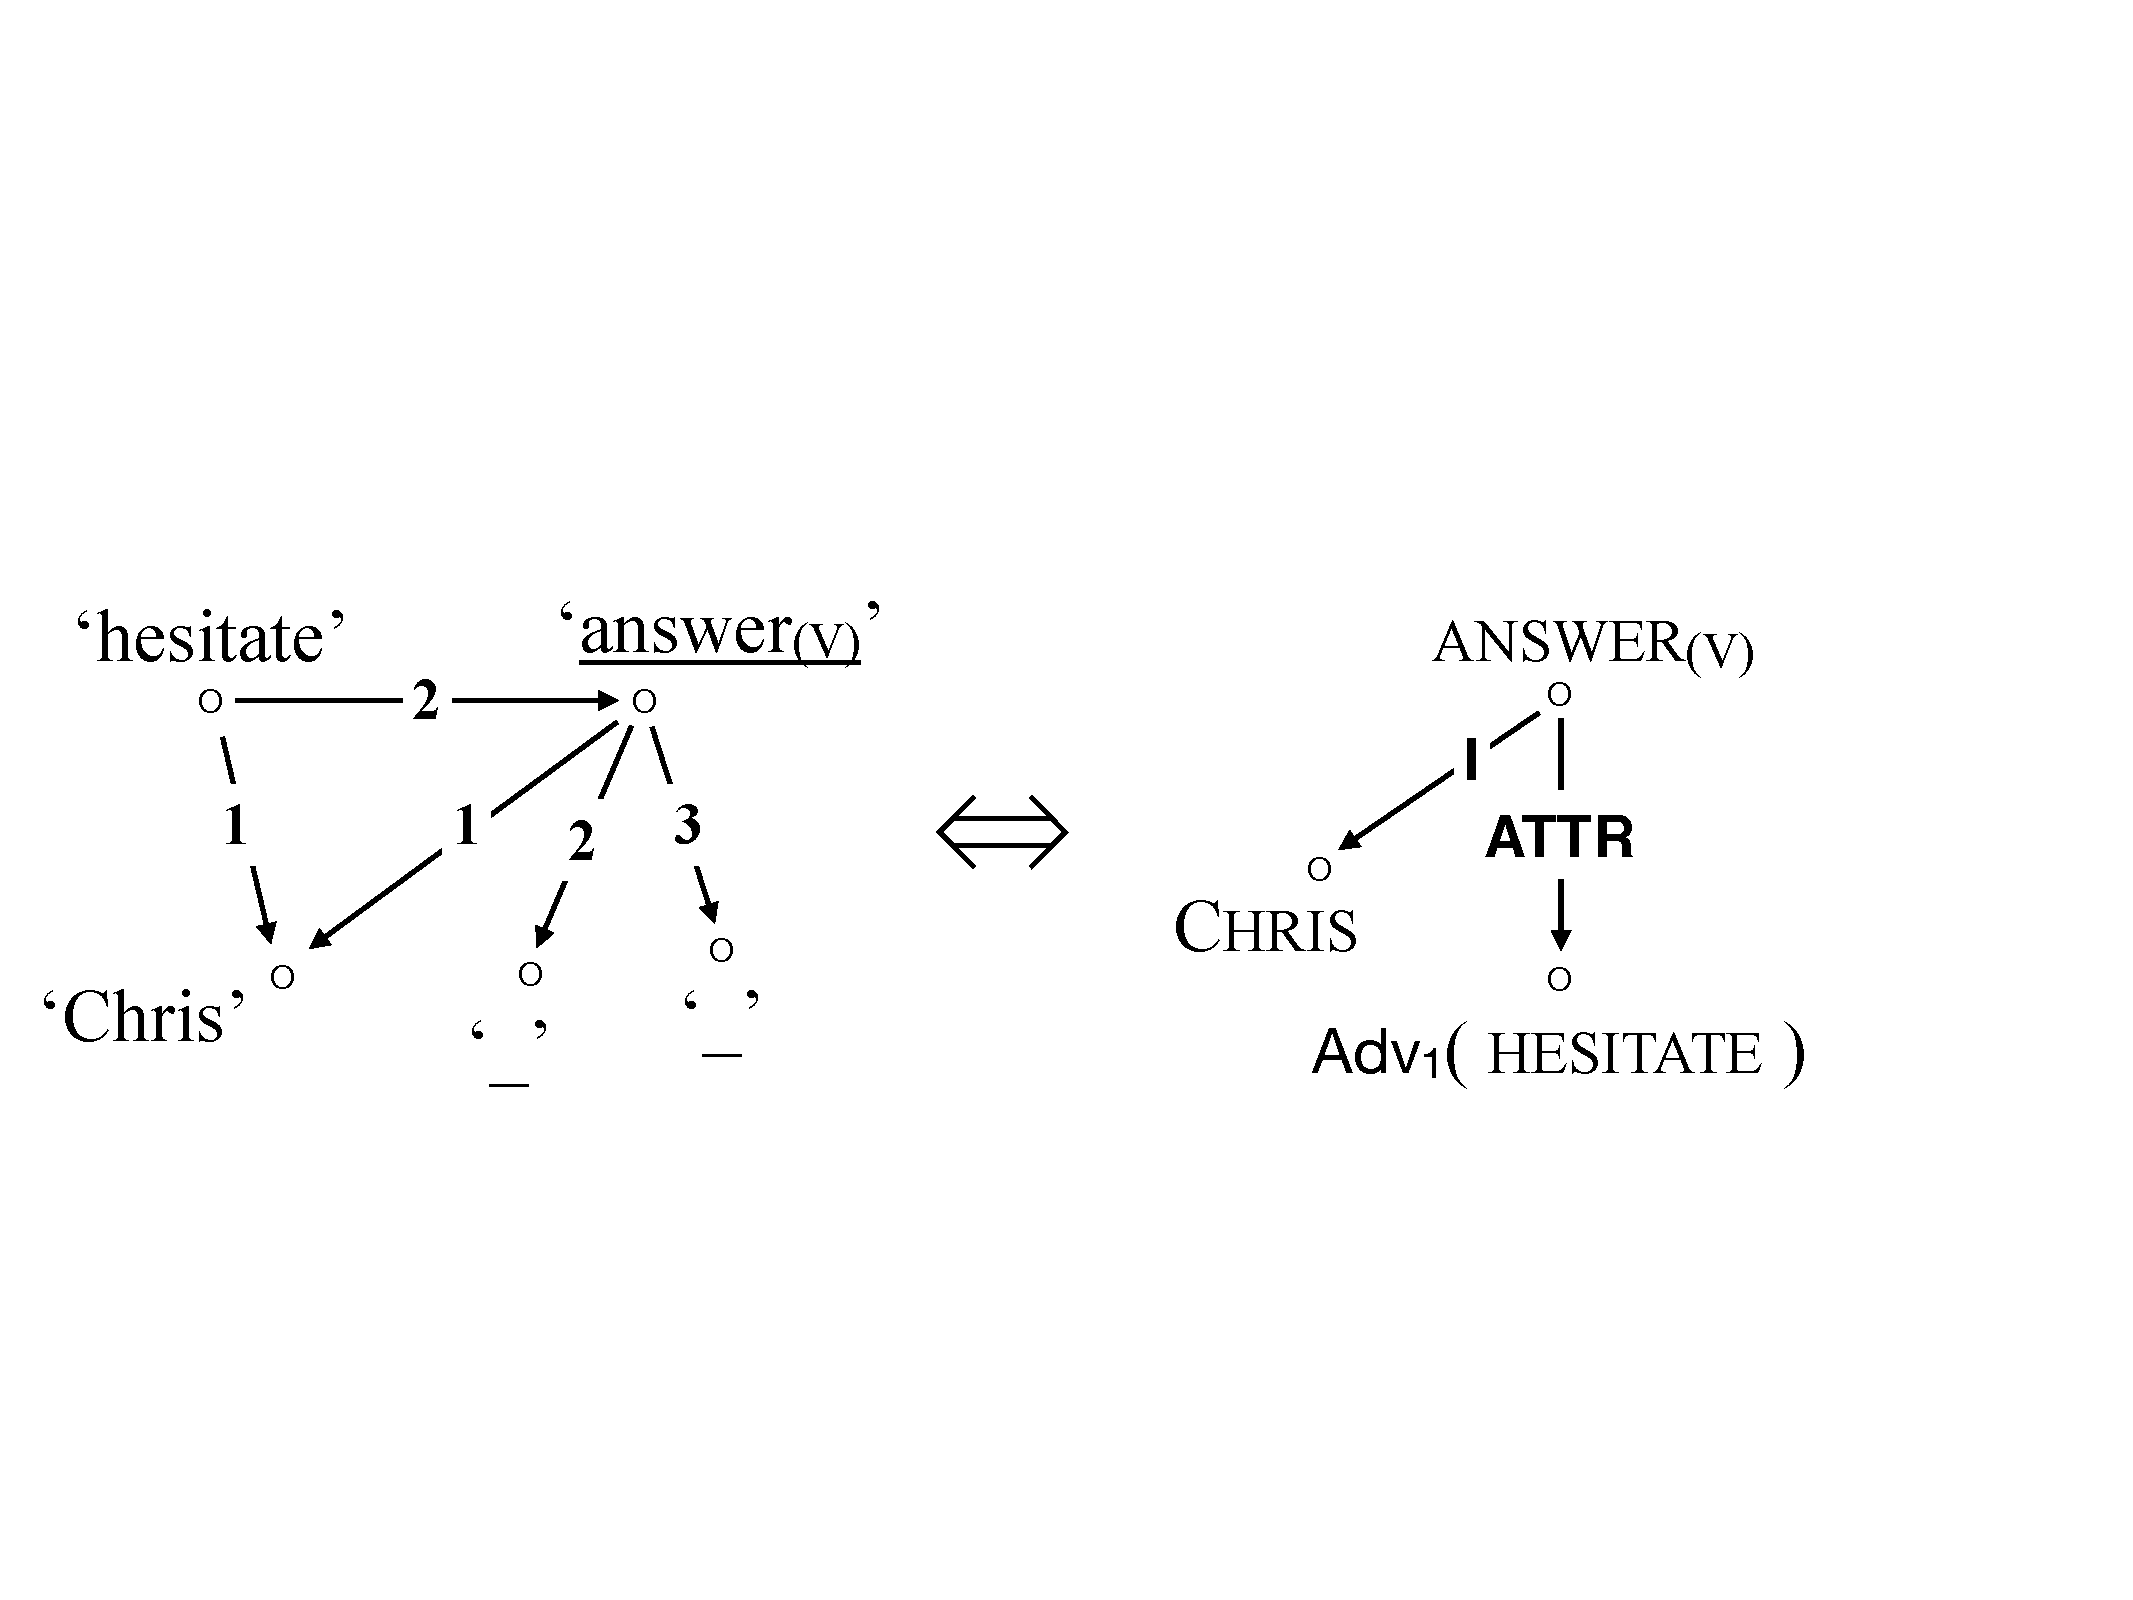
\includegraphics[width=9.5cm]{Fig/ParaLF/SemR-DSyntR-Adv1.pdf}
\caption{Sem\thinspace$\Leftrightarrow$\thinspace{}DSynt correspondence for the sentence \textit{Chris answers hesitatingly.}}\label{fig:Ch3-SemRDSyntR-Adv1}
\end{figure}

For \lfappl{Adv$_{2/3...}$}{L} things are more complicated since these adverbials involve a passive-like\index[notion]{voice, grammatical} use of L; for instance, see \Next, together with the corresponding Sem\thinspace$\Leftrightarrow$\thinspace{}DSynt correspondence in \figref{fig:Ch3-SemRDSyntR-Adv2}.

\begingroup
\small

\ex.\label{ex:ChapParaLF-ChrisFaintedUnderTheEyes} Chris fainted \emph{\idiom{under the eyes}}\tsub{\lfappl{Adv$_2$}{\textit{look}\tsub{(V)}}} of his uncle.

\endgroup

\begin{figure}

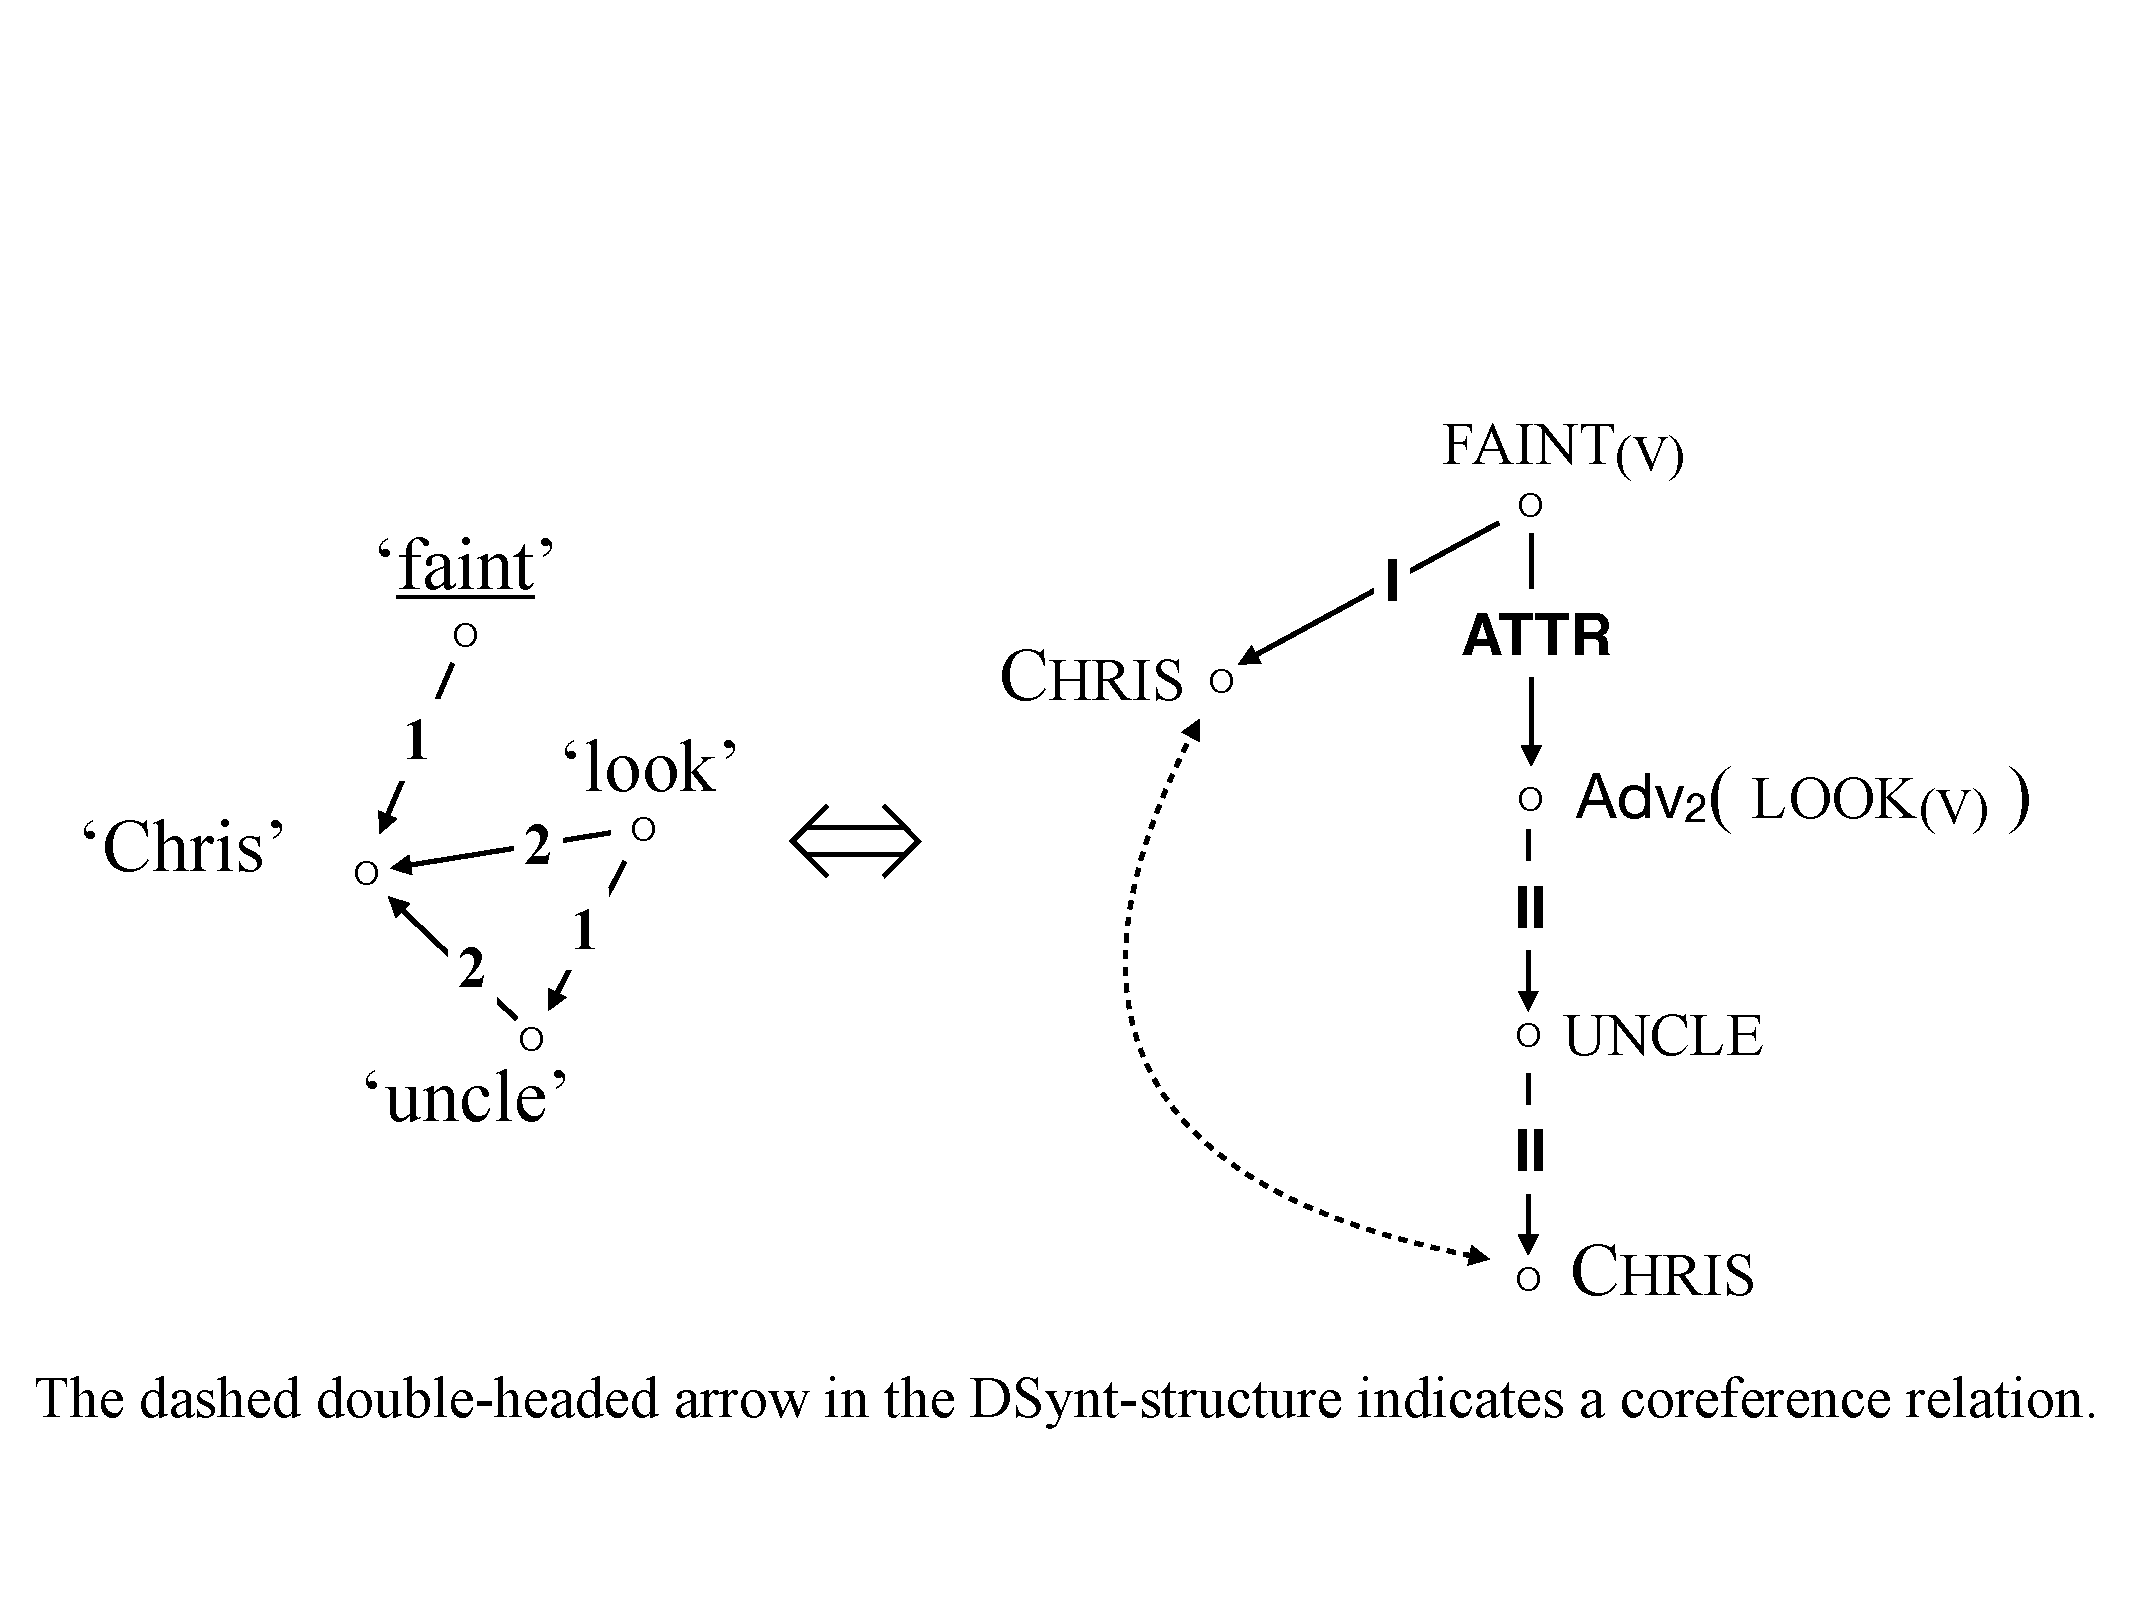
\includegraphics[width=9.5cm]{Fig/ParaLF/SemR-DSyntR-Adv2.pdf}
\caption{Sem\thinspace$\Leftrightarrow$\thinspace{}DSynt correspondence for the sentence \textit{Chris fainted under the eyes of his uncle.}}\label{fig:Ch3-SemRDSyntR-Adv2}
\end{figure}

In the DSynt-tree of \figref{fig:Ch3-SemRDSyntR-Adv2}, \textsc{uncle} appears as DSyntA\thinspace\syntDname{II} of \lfappl{Adv$_2$}{\textit{look}\tsub{(V)}} because this adverbial is equivalent to a passive form of \textsc{look}\tsub{(V)}: \idiom{\textit{under the eyes}} \textit{of his uncle}\enskip{\small $\equiv$}\enskip\textit{being looked at by his uncle}.

\paragraph*{Comment~2.}\label{para:comment2Advi}

A specific subset of lexical entities that are \lfappl{Adv\tsub{1}}{L} constitutes an exception to the statement in Comment~1: DSyntA\thinspace\syntDname{I} of these adverbials does not coincide with DSyntA\thinspace\syntDname{I} of the governing verb. Thus, in \Next, DSyntA\thinspace\syntDname{I} of \lf{Adv\tsub{1}} -- i.e. \textsc{Chris} -- does not coincide with DSyntA\thinspace\syntDname{I} of \textsc{vote}\tsub{(V)} -- i.e. \textsc{committee}:

\begingroup
\small

\ex. The committee voted \emph{in the absence} of Chris.

\endgroup

Other \lfappl{Adv\tsub{1}}{L} of the same type are \textit{in the presence} \lfgp{\textit{of} N\tsub{X}}, \textit{with the departure} \lfgp{\textit{of} N\tsub{X}}, \textit{with the illness}  \lfgp{\textit{of} N\tsub{X}}, etc.

All such adverbials are encoded by putting the \syntDname{1} actantial subscript\index[notion]{actantial subscript} between parentheses: \lfappl{Adv\tsub{(1)}}{L}\index[lf]{Advi@\lf{Adv\tsub{i}}!\lf{Adv\tsub{(i)}}|emph}. This notation indicates that the subscript does not do its normal job, but marks simultaneously two things:

\begin{itemize}

\item the non-coincidence between L's DSyntA\thinspace\syntDname{I} and that of the governing verb;

\item the obligatory character of the expression of L's DSyntA\thinspace\syntDname{I} with \lfappl{Adv\tsub{(1)}}{L}.

\end{itemize}

Consequently, the adverbial expression \textit{in the absence} in \Last is described by the LF formula \Next.

\begingroup
\small

\ex. \begingroup\setlength{\tabcolsep}{2pt}
\begin{tabular}[t]{ l l >{\raggedright\arraybackslash}p{6cm} }
\lfappl{Adv\tsub{(1)}}{\textit{absent}} & = & \textit{in the absence} \lfgp{\textit{of} N\tsub{X}} \\
\end{tabular}\endgroup

\endgroup

The \lf{Adv\tsub{1}} $\sim$ \lf{Adv\tsub{(1)}} contrast is parallel to the contrast between English regular V\tsub{\textsc{ing}} phrases with DSyntA\thinspace\syntDname{I} coinciding with DSyntA\thinspace\syntDname{I} of the governing verb \Next[a] and special V\tsub{\textsc{ing}} phrases whose DSyntA\thinspace\syntDname{I} does not \Next[b]:

\begingroup
\small

\ex. \a. \emph{Having left the house}, I heaved a sigh of relief.
     \b. \emph{My father having left the house}, I heaved a sigh of relief.

\endgroup

The V\tsub{\textsc{ing}} construction in \Last[b] is known as the \notion{absolute construction}\index[notion]{absolute construction}. Since \lf{Adv$_{(1)}$} lexical entities are, so to speak, the lexical embodiment of the absolute construction, it is convenient to call them \notion{absolutive adverbials}\index[notion]{adverb!absolutive \tld ial}.

\begin{historicalremark}
In several previous publications, \lf{Adv\tsub{i}} was erroneously classified as a syntagmatic LF -- see \textcite{Melcuk1982b}, \textcite{MelcukZholkovsky1984}, \textcite{Melcuketal1995-e} and \textcite{MelcukEtAl1999}.% The reason is that an element of an \lf{Adv\tsub{i}} is very often a preposition\index[notion]{preposition} governing a noun L, such as \textit{in silence} in the English illustrations on p.\thinspace\pageref{txt:Adv1IllustInSilence}.
\end{historicalremark}

\section{Singulative, collective and other inflection-like derivatives}\label{sec:flFlexion}

The LFs introduced in this section correspond to semantic derivatives manifesting a strong analogy with the expression of such inflectional\index[notion]{inflection} meanings as (noun) singular vs. plural, etc. These LFs come in two groups: (i)~those that have to do with quantity as regards L -- \lf{Sing} and \lf{Mult} -- and (ii) those that characterize the accomplishment of event L -- \lf{Imper}, \lf{Perf}, \lf{Imperf} and \lf{Result\tsub{i}}.

\refstepcounter{LFlist}
\subsubsection*{{\small [\arabic{LFlist}]} \lf{Sing} \lfgp{{\scriptsize Latin} \textit{singulus} `singular, unique'}: singulative}\label{lf:Sing}
\addcontentsline{toc}{subsection}{{\footnotesize [\arabic{LFlist}]} \lf{Sing}: singulative}\index[lf]{Sing@\lf{Sing}|emph}

\lfappl{Sing}{L} is a lexical entity that denotes a unit\slashs{}quantum of L's referent.

\begin{quote}
\begingroup
\small
\begin{tabular}{ l c c }
   \midrule
   \multicolumn{3}{l}{\lf{Sing}: verbal or nominal} \\
   \midrule
   \textbf{L} & V & N \\
   \midrule
   \textbf{\lfappl{Sing}{L}} & V & N \\
   \midrule
\end{tabular}
\endgroup
\end{quote}

\begin{longtable*}[l]{ l l >{\raggedright\arraybackslash}p{7cm} }

\multicolumn{3}{l}{\textbf{English}} \\*

\lfappl{S\tsub{0}Sing}{\textit{paint}\tsub{(V)}} & = & \idiom{\textit{brush stroke}} \\
\multicolumn{3}{ p{11cm} }{\leftskip=0.5cm{\small\remark{Note.}This is not a ``pure'' \lf{Sing} for a verb, but an \lf{S\tsub{0}Sing}, as it returns a nominal value. See the remark on verb singulatives after the illustrations.}} \\
\lfappl{Sing}{\textit{rice}} & = & \textit{grain of} \tld \\
\lfappl{Sing}{\textit{rain}\tsub{(N)}} & = & \textit{raindrop} \\
\lfappl{Sing}{\textit{parquet}} & = & \tld\ \textit{slat} \\
\lfappl{Sing}{\textit{body}} & = & \idiom{\textit{body part}} \\
\lfappl{Sing}{\textit{fur}\tsub{(N)}} & = & \textit{hair}\sensenum{3}\quad\lfgp{cf. \textit{hair}\sensenum{1} and \textit{hair}\sensenum{2} under \lf{Mult}, p.\thinspace\pageref{illustr:HAIR1-2}} \\
\lfappl{Sing}{\textit{vocabulary}} & = & \textit{word} \\[6pt]

\multicolumn{3}{l}{\textbf{French}} \\*

\lfappl{S\tsub{0}Sing}{\textit{peindre}} & = & \idiom{\textit{coup de pinceau}} \\
\lfappl{Sing}{\textit{riz}} & = & \textit{grain de} \tld \\
\lfappl{Sing}{\textit{pluie}} & = & \textit{goutte de} \tld \\
\lfappl{Sing}{\textit{parquet}} & = & \textit{lame de} \tld \\
\lfappl{Sing}{\textit{corps}} & = & \idiom{\textit{partie du corps}} \\
\lfappl{Sing}{\textit{pelage}} & = & \textit{poil} \\*
\lfappl{Sing}{\textit{vocabulaire}} & = & \textit{mot} \\[6pt]

\multicolumn{3}{l}{\textbf{Russian}} \\*

\lfappl{S\tsub{0}Sing}{\textit{pisat\palati} \lfgp{\textit{kartinu}}} & = & \textit{mazok} \\
\lfappl{Sing}{\textit{ris}} & = & \idiom{\textit{risovoe zërny\v{s}ko}}\textbf{,} \textit{risinka} \\
\lfappl{Sing}{\textit{do\v{z}d\suffixsplit\palati}} & = & \textit{kaplja} \tld\textit{ja} \\
\lfappl{Sing}{\textit{parket}} & = & \textit{parketina} \\
\lfappl{Sing}{\textit{telo}} & = & \idiom{\textit{\v{c}ast\palati\ tela}} \\
\lfappl{Sing}{\textit{mex}} & = & \textit{volos}\textbf{,} \textit{volosok} \\
\lfappl{Sing}{\textit{slovar\palati}} & = & \textit{slovo} \\

\end{longtable*}

In a \notion{Standard Average European} [SAE]\index[notion]{Standard Average European [SAE] language} language, the singulative typically applies to nouns, less frequently to verbs. Here are examples of verbal singulatives:

\begingroup
\small

\ex. \begingroup\setlength{\tabcolsep}{2pt}
\begin{tabular}[t]{ l l l >{\raggedright\arraybackslash}p{7cm} }
{\smaller English} & \lfappl{Sing}{\textit{beat}\tsub{(V)}} & = & \textit{hit}\tsub{(V)} \\
{\smaller French} & \lfappl{Sing}{\textit{battre}} & = & \textit{frapper} \\
{\smaller Russian} & \lfappl{Sing}{\textit{bit\palati}} & = & \textit{udarit\palati} \\
\end{tabular}\endgroup

\endgroup

Russian, with its inflectional category of aspect, has an important set of verbs whose perfective form expresses \lf{Sing}:

\begingroup
\small

\ex. \begingroup\setlength{\tabcolsep}{2pt}
\begin{tabular}[t]{ l l l l l }
\lfappl{Sing}{\textit{prygat\palati}} & `jump-\textsc{imperf}' & = & \textit{prygnut\palati} & `jump-\textsc{perf} = do one jump' \\
\lfappl{Sing}{\textit{udarjat\palati}} & `hit-\textsc{imperf}' & = & \textit{udarit\palati} & `hit-\textsc{perf} = give one blow' \\
\lfappl{Sing}{\textit{celovat\palati}} & `kiss-\textsc{imperf}' & = & \textit{pocelovat\palati} & `kiss-\textsc{perf} = give one kiss' \\
\end{tabular}\endgroup

\endgroup

\refstepcounter{LFlist}
\subsubsection*{{\small [\arabic{LFlist}]} \lf{Mult} \lfgp{{\scriptsize Latin} \textit{multum} `multitude'}: collective (for nouns)\slashs{}multiplicative (for verbs)}\label{lf:Mult}
\addcontentsline{toc}{subsection}{{\footnotesize [\arabic{LFlist}]} \lf{Mult}: collective (for nouns)\slashs{}multiplicative (for verbs)}\index[lf]{Mult@\lf{Mult}|emph}

\lfappl{Mult}{L} is a lexical entity that denotes a set of Ls forming a whole.

\begin{quote}
\begingroup

\begin{tabular}{ l c c }
   \midrule
   \multicolumn{3}{l}{\lf{Mult}: verbal or nominal} \\
   \midrule
   \textbf{L} & V & N \\
   \midrule
   \textbf{\lfappl{Mult}{L}} & V & N \\
   \midrule
\end{tabular}
\endgroup
\end{quote}

\phantomsection\label{illustr:HAIR1-2}\begin{longtable*}[l]{ l l >{\raggedright\arraybackslash}p{7cm} }

\multicolumn{3}{l}{\textbf{English}} \\*

\lfappl{Mult}{\textit{dog}} & = & \textit{pack}\tsub{(N)}\sensenum{II.1} \textit{of} \tld\textit{s} \\*
\lfappl{Mult}{\textit{lie}\tsub{(N)}} & = & \textit{pack}\tsub{(N)}\sensenum{II.4} \textit{of} \tld\textit{s} \\*
\lfappl{Mult}{\textit{hair}\sensenum{1}} & = & \textit{hair}\sensenum{2}\textbf{;} \idiom{\textit{head of hair}}\vspace{6pt} \\

\multicolumn{3}{l}{\textbf{French}} \\*

\lfappl{Mult}{\textit{chien}} & = & \textit{meute} \textit{de} \tld\textit{s} \\
\lfappl{Mult}{\textit{mensonge}} & = & \textit{tas} \textit{de} \tld\textit{s} \\
\lfappl{Mult}{\textit{cheveu}\sensenum{1}} & = & \textit{cheveux}\sensenum{2}\textbf{,} \textit{chevelure}\vspace{6pt} \\

\multicolumn{3}{l}{\textbf{Russian}} \\*

\lfappl{Mult}{\textit{sobak\suffixsplit{}a}} & = & \textit{svora} \tld \\
\lfappl{Mult}{\textit{l\suffixsplit{}o\v{z}\palati}} & = & \textit{ku\v{c}a} \tld\textit{\v{z}i} \\
\lfappl{Mult}{\textit{volos}\sensenum{1}} & = & \textit{volosy}\sensenum{2}\textbf{;} \textit{\v{s}eveljura} \\

\end{longtable*}

In parallel with singulative verbs, SAE languages\index[notion]{Standard Average European [SAE] language} show multiplicative verbs:\footnote{On the \lf{AntiMagn} LF used in \ref{ex:AntiMagn-Mult}, see \chapref{chap:syntLFs}, p.\thinspace\pageref{lf:AntiMagn}.}\index[lf]{AntiMagn@\lf{AntiMagn}}\index[lf]{Magn@\lf{Magn}!AntiMagn@\lf{AntiMagn}}

\begingroup
\small

\ex.\label{ex:AntiMagn-Mult} \begingroup\setlength{\tabcolsep}{2pt}
\begin{tabular}[t]{ l l l >{\raggedright\arraybackslash}p{6cm} }
{\smaller English} & \lfappl{AntiMagn+Mult}{\textit{jump}\tsub{(V)}} & = & \textit{hop}\tsub{(V)} \\
%French & \lfappl{AntiMagn\thinspace+\thinspace Mult}{\textit{sauter}} & = & \textit{sautiller} \\
{\smaller French} & \lfappl{AntiMagn+Mult}{\textit{taper}} & = & \textit{tapoter} \\
{\smaller Russian} & \lfappl{AntiMagn+Mult}{\textit{xlopat\palati}} & = & \textit{poxlopyvat\palati} \\
\end{tabular}\endgroup

\endgroup

\refstepcounter{LFlist}
\subsubsection*{{\small [\arabic{LFlist}]} \lf{Imper} \lfgp{{\scriptsize Latin} \textit{imper\={a}re} `[to] command, order'}: imperative}\label{lf:Imper}
\addcontentsline{toc}{subsection}{{\footnotesize [\arabic{LFlist}]} \lf{Imper}: imperative}\index[lf]{Imper@\lf{Imper}|emph}

\lfappl{Imper}{L} is an utterance by which the Speaker\index[notion]{Speaker, the} incites the Addressee\index[notion]{Addressee} to do L.

\begin{quote}
\begingroup
\small
\begin{tabular}{ l c }
   \midrule
   \multicolumn{2}{l}{\lf{Imper}: verbal or clausative\index[notion]{clausative}} \\
   \midrule
   \textbf{L} & V \\
   \midrule
   \textbf{\lfappl{Imper}{L}} & V\slashs{}Claus \\
   \midrule
\end{tabular}
\endgroup
\end{quote}

\begin{longtable*}[l]{ l l >{\raggedright\arraybackslash}p{6.5cm} }

\multicolumn{3}{l}{\textbf{English}} \\*

\lfappl{Imper}{\idiom{\textit{go away}}} & = & \uslabel{colloquial} \idiom{\textit{Beat it!}} \\
\lfappl{ImperPred}{\textit{quiet}\tsub{(Adj)}} & = & \textit{Quiet!}\textbf{,} \textit{Shush!}\textbf{,} \textit{Shh!} \\
\lfappl{Imper}{\idiom{\textit{give up}}} & = & \idiom{\textit{Let it go!}} \\
\lfappl{Imper}{\textit{Bang!}} & = & \textit{Fire!} \\
\lfappl{ImperPrepar\tsub{1}Real\tsub{1}}{\textit{meal}} & = & \textit{Breakfast} $\langle$\textit{Lunch} $\rangle$ $\langle$\textit{Supper}$\rangle$ \textit{is ready!} \\[6pt]

\multicolumn{3}{l}{\textbf{French}} \\*

\lfappl{Imper}{\textit{partir}} & = & \uslabel{offensive} \textit{Dégage !}\textbf{;} \uslabel{colloquial} \textit{Zou !} \\
\lfappl{Imper}{\textit{se taire}} & = & \textit{Chut !}\textbf{;} \uslabel{offensive} \idiom{\textit{Ta gueule !}} \\
\lfappl{Imper}{\idiom{\textit{tenir le coup}}} & = & \textit{Courage !} \\
\lfappl{Imper}{\textit{venir}} & = & \textit{Ici !} \\
\lfappl{Imper\tsub{$\supset$}}{\idiom{\textit{laisser le passage}}} & = & \idiom{\textit{Chaud devant !}} \\
\lfappl{Imper}{\textit{Pan !}} & = & \textit{Feu !} \\
\lfappl{Imper}{\textit{abandonner}} & = & \idiom{\textit{Laisse tomber !}} \\*
\lfappl{ImperPrepar\tsub{1}Real\tsub{1}}{\textit{repas}} & = & \textit{À table !} \\[6pt]

\multicolumn{3}{l}{\textbf{Russian}} \\*

\lfappl{Imper}{\textit{ujti}} & = & \uslabel{offensive} \textit{Von} (\textit{otsjuda})\textit{!}\textbf{,} \uslabel{colloquial offensive} \textit{Po\v{s}ël von} (\textit{otsjuda})\textit{!} \\
\lfappl{Imper}{\textit{ne \v{s}umet\palati}} & = & \textit{Tixo!}\textbf{,} \textit{Tss!}\textbf{,} \textit{T\v{s}\v{s}!} \\
\lfappl{Imper}{\textit{vzjat\palati}} & = & \textit{Na}(\textit{te})\textit{!} \\*
\lfappl{Imper}{\uslabel{child language} \textit{Pif-paf!}} & = & \textit{Ogon\palati!} \\
\lfappl{ImperPrepar\tsub{1}Real\tsub{1}}{\textit{eda}} & = & (\textit{Pro\v{s}u vsex}) \textit{za stol!}\textbf{,} (\textit{Pro\v{s}u vsex}) \textit{k stolu!} \\

\end{longtable*}

\refstepcounter{LFlist}
\subsubsection*{{\small [\arabic{LFlist}]} \lf{Perf} \lfgp{{\scriptsize Latin} \textit{perfectum}}: perfective}\label{lf:Perf}
\addcontentsline{toc}{subsection}{{\footnotesize [\arabic{LFlist}]} \lf{Perf}: perfective}\index[lf]{Perf@\lf{Perf}|emph}

\lfappl{Perf}{L} is a verbal or clausative\index[notion]{clausative} lexical unit that denotes the fact of reaching the goal\verythinspace/\verythinspace{}limit inherent to the meaning of L -- cf. the comment that follows the illustrations for the LF \lf{Result\tsub{i}} below ([\ref{lf:Result-i}], p.\thinspace\pageref{txt:ResultvsPerf}).

\lf{Perf} and the following LF \lf{Imperf}\index[lf]{Imperf@\lf{Imperf}} correspond to aspectual meanings grammaticalized in Slavic languages, where they are inflectional\index[notion]{inflection}.

\begin{quote}
\begingroup
\small
\begin{tabular}{ l c }
   \midrule
   \multicolumn{2}{l}{\lf{Perf}: verbal or clausative} \\
   \midrule
   \textbf{L} & V \\
   \midrule
   \textbf{\lfappl{Perf}{L}} & V\slashs{}Claus \\
   \midrule
\end{tabular}
\endgroup
\end{quote}

\begin{longtable*}[l]{ l l >{\raggedright\arraybackslash}p{6cm} }

\multicolumn{3}{l}{\textbf{English}} \\*

\lfappl{Perf}{\textit{end}\tsub{(V)}} & = & \idiom{\textit{be over}} \\
\lfappl{Perf}{\textit{undress}} & = & \textit{have undressed} \\
\lfappl{Claus\tsub{0}Perf}{\textit{dive}\tsub{(V)}}\index[lf]{Claus0Perf@\lf{Claus\tsub{0}Perf}} & = & \textit{Splash!} \\[6pt]

\multicolumn{3}{l}{\textbf{French}} \\*

\lfappl{Perf}{\textit{revenir}} & = & \idiom{\textit{être de retour}} \\
\lfappl{Perf}{\textit{se déshabiller}} & = & \textit{s'être déshabillé} \\
\lfappl{Claus\tsub{0}Perf}{\textit{plonger}} & = & \textit{Plouf !} \\[6pt]

\multicolumn{3}{l}{\textbf{Russian}} \\*

\lfappl{Perf}{\textit{razdevat\palati{}sja}}  & = & \textit{razdet\palati{}sja} \\
\lfappl{Perf}{\textit{odevat\palati{}sja}}  & = & \textit{odet\palati{}sja} \\
\lfappl{Claus\tsub{0}Perf}{\textit{padat\palati} \lfgp{in a liquid}}  & = & \textit{Bux!}\textbf{,} \textit{Pljux!} \\

\end{longtable*}

Values of \lfappl{Perf}{L} and \lfappl{Imperf}{L} are mostly trivial, in the sense that they are usually grammatical forms of a verb L. \lf{Perf} is mainly used in complex LF formulas such as \lf{S\tsub{i}Perf}\phantomsection\label{lf:S-iPerf}\index[lf]{Si@\lf{S\tsub{i}}}, \lf{A\tsub{i}Perf}\phantomsection\label{lf:A-iPerf}\index[lf]{Ai@\lf{A\tsub{i}}} or \lf{PerfOper\tsub{i}}\phantomsection\label{lf:PerfOper-i}\index[lf]{Operi@\lf{Oper\tsub{i}}}.

\begingroup
\small

\ex. \begingroup\setlength{\tabcolsep}{2pt}
\begin{tabular}[t]{ l l >{\raggedright\arraybackslash}p{7cm} }
\lfappl{S\tsub{1}Perf}{\idiom{\textit{give birth}}} & = & \idiom{\textit{new mother}} \\
\lfappl{A\tsub{2}Perf}{\textit{cook}\tsub{(V)}} & = & \textit{cooked} \\
\lfappl{PerfOper{\tsub{1}}}{\textit{divorce}\tsub{(N)}} & = & \textit{get} \lfgp{\textsc{art} \tld} \\
\end{tabular}\endgroup

\endgroup

\refstepcounter{LFlist}
\subsubsection*{{\small [\arabic{LFlist}]} \lf{Imperf} \lfgp{{\scriptsize Latin} \textit{imperfectum}}: imperfective}\label{lf:Imperf}
\addcontentsline{toc}{subsection}{{\footnotesize [\arabic{LFlist}]} \lf{Imperf}: imperfective}\index[lf]{Imperf@\lf{Imperf}|emph}

\lfappl{Imperf}{L} is a verbal or clausative\index[notion]{clausative} lexical unit that denotes fact L as ongoing process and, eventually (as in Slavic languages), as the iteration of fact L.

\begin{quote}
\begingroup
\small
\begin{tabular}{ l c }
   \midrule
   \multicolumn{2}{l}{\lf{Imperf}: verbal or clausative} \\
   \midrule
   \textbf{L} & V \\
   \midrule
   \textbf{\lfappl{Imperf}{L}} & V\slashs{}Claus \\
   \midrule
\end{tabular}
\endgroup
\end{quote}

\begin{longtable*}[l]{ l l >{\raggedright\arraybackslash}p{6cm} }

\multicolumn{3}{l}{\textbf{English}} \\*

\lfappl{Imperf}{\idiom{\textit{be over}}} & = & \textit{end}\tsub{(V)}\textbf{,} \textit{finish}\tsub{(V)}\vspace{6pt} \\

\multicolumn{3}{l}{\textbf{French}} \\*

\lfappl{Imperf}{\textit{se réveiller}} & = & \uslabel{colloquial} \textit{émerger}\vspace{6pt} \\

\multicolumn{3}{l}{\textbf{Russian}} \\*

\lfappl{Imperf}{\textit{vernut\palati{}sja}}  & = & \textit{vozvra\v{s}\v{c}at\palati{}sja} \\
\lfappl{Imperf}{\textit{odet\palati{}sja}}  & = & \textit{odevat\palati{}sja} \\

\end{longtable*}

\refstepcounter{LFlist}
\subsubsection*{{\small [\arabic{LFlist}]} \lf{Result\tsub{i}} \lfgp{{\scriptsize Latin} *\textit{result\={a}re} `[to] result'}: resultative}\label{lf:Result-i}
\addcontentsline{toc}{subsection}{{\footnotesize [\arabic{LFlist}]} \lf{Result\tsub{i}}: resultative}\index[lf]{Resulti@\lf{Result\tsub{i}}|emph}

\lfappl{Result\tsub{i}}{L} is a verbal or clausative\index[notion]{clausative} lexical unit that denotes a situation \emph{necessarily} resulting from reaching the goal\slashs{}limit inherent to the meaning of L. DSyntA\thinspace\syntDname{I} of \lfappl{Result\tsub{i}}{L} corresponds to DSyntA\thinspace\syntDname{i} of L.

Let it be emphasized that the situation denoted by \lfappl{Result\tsub{i}}{L} is the necessary result of reaching L's goal\slashs{}limit. This is in contrast with some cases of \lfappl{Real\tsub{i}}{L}\index[lf]{Reali@\lf{Real\tsub{i}}} that are considered in \chapref{chap:syntLFs} (\sectref{sec:verbeReal}, [\ref{lf:Real-i}], ``\nameref*{par:RealVFusion},'' p.\thinspace\pageref{par:RealVFusion}), where the situation referred to by \lfappl{\lf{Real\tsub{i}}}{L} can be achieved in different ways.

\begin{quote}
\begingroup
\small
\begin{tabular}{ l c }
   \midrule
   \multicolumn{2}{l}{\lf{Result\tsub{i}}: verbal or clausative} \\
   \midrule
   \textbf{L} & V  \\
   \midrule
   \textbf{\lfappl{Result\tsub{i}}{L}} & V\slashs{}Claus \\
   \midrule
\end{tabular}
\endgroup
\end{quote}

\begin{longtable*}[l]{ l l >{\raggedright\arraybackslash}p{5cm} }

\multicolumn{3}{l}{\textbf{English}} \\*

\lfappl{Result\tsub{1}}{\textit{reach}\tsub{(V)} \lfgp{N\tsub{Y}}} & = & \textit{be} \lfgp{\lf{Loc\tsub{in}} N\tsub{Y}} \\[1pt]
\multicolumn{3}{ p{11cm} }{\leftskip=0.5cm{\small\remark{Note.}For the syntagmatic LF \lf{Loc\tsub{in}} (locative preposition meaning `being located in'), see \chapref{chap:syntLFs}, [\ref{lf:Loc-in}], p.\thinspace\pageref{lf:Loc-in}.}}\index[lf]{Locin@\lf{Loc\tsub{in}}} \\[1pt]
\lfappl{Result\tsub{1}}{\uslabel{colloquial} \idiom{\textit{drift off}}} & = & \textit{sleep}\tsub{(V)}\textbf{;} \textit{Zzz!} \\
\lfappl{Result\tsub{1}}{\textit{agonize}} & = & \textit{die}\tsub{(V)} \\
\lfappl{Result\tsub{1}}{\textit{die}\tsub{(V)}} & = & \uslabel{colloquial} \idiom{\textit{push up daisies}} \\
\lfappl{Result\tsub{1}}{\textit{acquire}} & = & \textit{own}\tsub{(V)} \\*
\lfappl{Result\tsub{2}}{\uslabel{colloquial} \idiom{\textit{shut up}}\sensenum{2} \lfgp{N\tsub{Y}}} & = & \uslabel{colloquial} \lfgp{N\tsub{Y}} \idiom{\textit{shut up}}\sensenum{1} \\[6pt]

\multicolumn{3}{l}{\textbf{French}} \\*

%%%\lfappl{Result\tsub{1}}{\textit{s'approcher} \lfgp{\textit{de} N\tsub{Y}}} & = & \textit{atteindre} \lfgp{N\tsub{Y}} \\ @@@ Real1 ?
\lfappl{Result\tsub{1}}{\textit{atteindre} \lfgp{N\tsub{Y}}} & = & \textit{être} \lfgp{\lf{Loc\tsub{in}} N\tsub{Y}} \\
\lfappl{Result\tsub{1}}{\textit{s'endormir}} & = & \textit{dormir}\textbf{;} \textit{Zzz~!} \\
\lfappl{Result\tsub{1}}{\textit{agoniser}} & = & \textit{mourir} \\
\lfappl{Result\tsub{1}}{\textit{mourir}} & = & \uslabel{colloquial} $\ulcorner$\textit{manger les pissenlits par la racine}$\urcorner$ \\
\lfappl{Result\tsub{1}}{\textit{acquérir}} & = & \textit{posséder} \\
\lfappl{Result\tsub{2}}{\uslabel{colloquial} \idiom{\textit{clouer le bec}} \lfgp{\textit{à} N\tsub{Y}}} & = & \lfgp{N\tsub{Y}} \textit{se taire} \\[6pt]
%\lfappl{\lf{S\tsub{0}}Result\tsub{1}}{\textit{se souler}} & = & \idiom{\textit{gueule de bois}} \\ Intéressant, mais ce n'est pas une situation résultant NÉCESSAIREMENT du fait de se saouler.

\multicolumn{3}{l}{\textbf{Russian}} \\*

\lfappl{Result\tsub{1}}{\textit{dosti\v{c}\palati} \lfgp{N\tsub{Y-\textsc{gen}}}} & = & \textit{byt\palati} \lfgp{\lf{Loc\tsub{in}} N\tsub{Y}} \\
\lfappl{Result\tsub{1}}{\textit{zasnut\palati}} & = & \textit{spat\palati}\textbf{;} \textit{Xrrr...!} \\
\lfappl{Result\tsub{1}}{\textit{agonizirovat\palati}} & = & \textit{umeret\palati} \\
\lfappl{Result\tsub{1}}{\textit{umeret\palati}} & = & \uslabel{colloquial} \idiom{\textit{byt\palati na tom svete}} \\
\lfappl{Result\tsub{1}}{\textit{priobresti}} & = & \textit{vladet\palati} \\
\lfappl{Result\tsub{2}}{\uslabel{colloquial} \idiom{\textit{zatknut\palati\ rot}} \lfgp{N\tsub{Y-\textsc{dat}}}} & = & \lfgp{N\tsub{Y-\textsc{nom}}} \textit{zamol\v{c}at\palati}\textbf{,} \uslabel{colloquial} \textit{zatknut\palati{}sja}\textbf{;} \textit{Ni\onewdf{}gugu}\tsub{(Interj)} \\

\end{longtable*}

\phantomsection\label{txt:ResultvsPerf}\lf{Result\tsub{i}} must be distinguished from \lf{Perf}\index[lf]{Perf@\lf{Perf}}, for which it could be mistaken. For instance, \Next[a] has a different meaning from \Next[b]:

\begingroup
\small

\ex. \a. \textit{have reached}\tsub{\lfappl{Perf}{\textit{reach}\tsub{(V)}}} \textit{Montreal}
     \b. \textit{be}\tsub{\lfappl{Result\tsub{1}}{\textit{reach}\tsub{(V)}}} \textit{in Montreal}

\endgroup

\lfappl{Perf}{L} denotes the same fact as L but in a different state: `have reached' is still `reach', but `completed'. On the contrary, \lfappl{Result\tsub{i}}{L} denotes a different fact: the situation which is necessarily entailed by reaching L's goal\verythinspace/\verythinspace{}limit and in which L's DSyntA\thinspace\syntDname{i} finds itself. 

\clearpage{\pagestyle{empty}\cleardoublepage}


% !TEX root = LF-IMAPol.tex

\chapter{Syntagmatic lexical functions}\label{chap:syntLFs}

Syntagmatic LFs\index[notion]{syntagmatic!\tld\ lexical function}\index[notion]{lexical function!syntagmatic \tld}\index[notion]{syntagmatic!\tld\ lexical function} are grouped into four major classes according to their part of speech\index[notion]{lexical function!part of speech of a \tld}\index[notion]{part of speech [PoS]!\tld\ of an LF} [PoS] -- i.e., the PoS of the collocate\index[notion]{collocation!collocate of a \tld} they encode. They are presented below in the same order\index[notion]{lexical function!ordering of \tlds}\index[notion]{ordering of LFs} as in the cooccurrence zone\index[notion]{lexical entry!cooccurence zone of a \tld}\index[notion]{zone of a lexical entry!cooccurrence \tld} of a lexical entry\index[notion]{lexicography} (where they appear after paradigmatic LFs):

\begin{itemize}

\item \nameref*{sec:collocNominauxEtatsL} (\sectref{sec:collocNominauxEtatsL})

\item \nameref*{sec:collocatifsModif} (\sectref{sec:collocatifsModif})

\item \nameref*{sec:collocatifsPrepositionnels} (\sectref{sec:collocatifsPrepositionnels})

\item \nameref*{sec:verbalCollocates}, distributed into seven subclasses corresponding to their increasing semantic load -- i.e., the richness of their meaning \sigmaF\ (\sectref{sec:verbalCollocates})

\begin{itemize}\vspace{-5pt}

\item[--] \nameref*{sec:verbeCopule} (\sectref{sec:verbeCopule})

\item[--] \nameref*{sec:verbeSupport} (\sectref{sec:verbeSupport})

\item[--] \nameref*{sec:verbeReal} (\sectref{sec:verbeReal})

\item \nameref*{sec:phasicVerbs} (\sectref{sec:phasicVerbs})

%\item[--] \nameref*{sec:collocatifsVerbesPhasiques} (\ref{sec:collocatifsVerbesPhasiques})

\item[--] \nameref*{sec:collocCausatif} (\sectref{sec:collocCausatif})

\item[--] \nameref*{sec:FLmodeFonct} (\sectref{sec:FLmodeFonct})

\item[--] \nameref*{sec:autresCollocatifsVerbaux} (\sectref{sec:autresCollocatifsVerbaux})

\end{itemize}

\end{itemize}

We conclude this chapter with a summary of alternative approaches to the description of collocations\index[notion]{collocation}, with a focus on lexicographic models -- dictionaries\index[notion]{dictionary} and lexical databases\index[notion]{lexical database} (\sectref{sec:Non-LFApproachesCollocations}).

\section{Nominal collocates} \label{sec:collocNominauxEtatsL}

The two nominal collocates -- \lf{Germ} and \lf{Culm} -- are syntactic governors of L.

\refstepcounter{LFlist}
\subsubsection*{{\small [\arabic{LFlist}]} \lf{Germ} \lfgp{{\scriptsize Latin} \textit{germen} `embryo'}: origin}\label{lf:Germ}
\addcontentsline{toc}{subsection}{{\footnotesize [\arabic{LFlist}]} \lf{Germ}: origin}\index[lf]{Germ@\lf{Germ}|emph}

\lfappl{Germ}{L} is a nominal lexical unit that denotes L's initial state, that is, something that will become L.

\begin{quote}
\begingroup
\small
\begin{tabular}{ l c }
   \midrule
   \multicolumn{2}{l}{\lf{Germ}: nominal} \\
   \midrule
   \textbf{L} & N \\
   \midrule
   \textbf{\lfappl{Germ}{L}} & N \\
   \midrule
\end{tabular}
\endgroup
\end{quote}

\begin{longtable*}[l]{ l l >{\raggedright\arraybackslash}p{7cm} }

\multicolumn{3}{l}{\textbf{English}} \\*

\lfappl{Germ}{\textit{flower}\tsub{(N)}} & = & \lfgp{\tld} \textit{bud} \\
\lfappl{Germ}{\lfgp{\textit{a}} \textit{painting}} & = & \textit{sketch} \lfgp{\textit{of} \textsc{art} \tld} \\
\lfappl{Germ}{\textit{idea}} & = & \textit{germ} \lfgp{\textit{of} (\textsc{art}) \tld} \\[6pt]

\multicolumn{3}{l}{\textbf{French}} \\*

\lfappl{Germ}{\textit{fleur}} & = & \textit{bouton} \lfgp{\textit{de} (\textsc{art}) \tld} \\
\lfappl{Germ}{\lfgp{\textit{une}} \textit{peinture}} & = & \textit{esquisse} \lfgp{\textit{de} \textsc{art} \tld} \\
\lfappl{Germ}{\textit{idée}} & = & \textit{embryon}\textbf{,} \textit{germe} \lfgp{\textit{de} (\textsc{art}) \tld} \\[6pt]

\multicolumn{3}{l}{\textbf{Russian}} \\*

\lfappl{Germ}{\textit{cvet\suffixsplit{}ok}} & = & \textit{buton} \lfgp{\tld\textit{ka}} \\
\lfappl{Germ}{\textit{kartin\suffixsplit{}a}} & = & \textit{nabrosok} \lfgp{\tld\textit{y}} \\
\lfappl{Germ}{\textit{ide\suffixsplit{}ja}} & = & \textit{zarody\v{s}} \lfgp{\tld\textit{i}} \\

\end{longtable*}

\refstepcounter{LFlist}
\subsubsection*{{\small [\arabic{LFlist}]} \lf{Culm} \lfgp{{\scriptsize Latin} \textit{culmen} `highest point'}: culmination}\label{lf:Culm}
\addcontentsline{toc}{subsection}{{\footnotesize [\arabic{LFlist}]} \lf{Culm}: culmination}\index[lf]{Culm@\lf{Culm}|emph}

\lfappl{Culm}{L} is a nominal lexical unit that denotes L's culminating\slashs{}central point. 

\begin{quote}
\begingroup
\small
\begin{tabular}{ l c }
   \midrule
   \multicolumn{2}{l}{\lf{Culm}: nominal} \\
   \midrule
   \textbf{L} & N \\
   \midrule
   \textbf{\lfappl{Culm}{L}} & N \\
   \midrule
\end{tabular}
\endgroup
\end{quote}

\begin{longtable*}[l]{ l l >{\raggedright\arraybackslash}p{7cm} }

\multicolumn{3}{l}{\textbf{English}} \\*

\lfappl{Culm}{\textit{anger}\tsub{(N)}} & = & \textit{paroxysm} \lfgp{\textit{of} (\textsc{art}) \tld} \\
\lfappl{Culm}{\textit{crisis}} & = & \textit{apogee}\textbf{,} \textit{peak} \lfgp{\textit{of} \textsc{art} \tld} \\
\lfappl{Culm}{\textit{problem}} & = & \textit{crux}\textbf{,} \textit{heart}  \lfgp{\textit{of} \textsc{art} \tld} \\
\lfappl{Culm}{\textit{night}} & = & \textit{dead} \lfgp{\textit{of} (\textit{the}) \tld} \\
\lfappl{Culm}{\textit{earthquake}} & = & \uslabel{specialized} \textit{focus}\textbf{,} \uslabel{specialized} \textit{hypocenter} \lfgp{\textit{of} \textsc{art}~\tld}\textbf{;} \uslabel{(specialized)}
~\textit{epicenter} \lfgp{\textit{of} \textsc{art}~\tld} \\
\lfappl{Culm}{\textit{cyclone}} & = & \textit{center}\textbf{,} \textit{eye} \lfgp{\textit{of} \textsc{art}~\tld} \\[1pt]
\multicolumn{3}{ >{\raggedright\arraybackslash}p{11.5cm} }{\leftskip=0.5cm{\small\remark{Notes.}The usage label \uslabel{(specialized)} indicates that \textit{epicenter} is a ``runaway term,''\index[notion]{runaway term}\index[notion]{terminology} i.e., a full-fledged term that nonetheless tends to be used in non-specialized discourse by speakers
who do not necessarily master the corresponding terminological notion \parencite[10]{GotkovaEtAl2024}. The phrases \textit{center}\slashs\textit{eye} \lfgp{\textit{of a cyclone}} -- cf. \lfappl{Culm}{\textit{cyclone}} -- denote the central part of a cyclone where the intensity of the wind is minimal, but which is seen as the most dangerous place to be in.
}} \\[6pt]

\multicolumn{3}{l}{\textbf{French}} \\*

\lfappl{Culm}{\textit{colère}} & = & \textit{paroxysme} \lfgp{\textit{de} \textsc{art} \tld} \\
\lfappl{Culm}{\textit{joie}} & = & \textit{comble} \lfgp{\textit{de} \textsc{art} \tld} \\
\lfappl{Culm}{\textit{problème}} & = & \textit{cœur}\textbf{,} \textit{noyau}  \lfgp{\textit{de} \textsc{art} \tld} \\
\lfappl{Culm}{\textit{nuit}} & = & \textit{cœur} \lfgp{\textit{de} \textsc{art} \tld} \\
\lfappl{Culm}{\idiom{\textit{tremblement de terre}}} & = & \textit{foyer}\textbf{,} \uslabel{specialized} \textit{hypocentre} \lfgp{\textit{de} \textsc{art} \tld}\textbf{;} \uslabel{(specialized)}~\textit{épicentre} \lfgp{\textit{de} \textsc{art}~\tld} \\
\lfappl{Culm}{\textit{cyclone}} & = & \textit{œil} \lfgp{\textit{de} \textsc{art} \tld} \\[6pt]

\multicolumn{3}{l}{\textbf{Russian}} \\*

\lfappl{Culm}{\textit{ciklon}} & = & \textit{glaz}\textbf{,} \textit{oko} \lfgp{\tld\textit{a}} \\
\lfappl{Culm}{\textit{zemletrjaseni\suffixsplit{}e}} & = & \textit{èpicentr}\textbf{,} \textit{o\v{c}ag} \lfgp{\tld\textit{ja}}\textbf{;} \uslabel{specialized} \textit{gipocentr} \lfgp{\tld\textit{ja}} \\
\lfappl{Culm}{\textit{problem\suffixsplit{}a}} & = & \textit{sut\palati} \lfgp{\tld\textit{y}} \\

\end{longtable*}

\lf{Culm} often appears in combination with the syntagmatic LF \lf{Loc\tsub{in}}\index[lf]{Locin@\lf{Loc\tsub{in}}} (\sectref{sec:collocatifsPrepositionnels}, [\ref{lf:Loc-in}], p.\thinspace\pageref{lf:Loc-in}), forming a complex LF\index[notion]{lexical function!complex \tld}:

\phantomsection\label{txt:inDeadOfNight}\begin{longtable*}[l]{ l l >{\raggedright\arraybackslash}p{6cm} }

\multicolumn{3}{l}{\textbf{English}} \\*

\lfappl{Loc\tsub{in}Culm}{\textit{night}} & = & \textit{in the dead} \lfgp{\textit{of} (\textit{the}) \tld} \\
\lfappl{Loc\tsub{in}Culm}{\textit{storm}} & = & \textit{at the heart} \lfgp{\textit{of} \textsc{art} \tld} \\[6pt]

\multicolumn{3}{l}{\textbf{French}} \\*

\lfappl{Loc\tsub{in}Culm}{\textit{nuit}} & = & \idiom{\textit{en pleine}} \lfgp{\tld}\textbf{,} \idiom{\textit{au plus noir}} \lfgp{\textit{de la} \tld}\\
\lfappl{Loc\tsub{in}Culm}{\textit{saison} \lfgp{\textit{touristique}}} & = & \idiom{\textit{au plus gros}} \lfgp{\textit{de la} \tld} \\[6pt]

\multicolumn{3}{l}{\textbf{Russian}} \\*

\lfappl{Loc\tsub{in}Culm}{\textit{sezon}} & = & \textit{v} (\textit{samyj}) \textit{razgar} \lfgp{\tld\textit{a}} \\
\lfappl{Loc\tsub{in}Culm}{\textit{slav\suffixsplit{}a}} & = & \textit{na ver\v{s}ine} \lfgp{\tld\textit{y}} \\

\end{longtable*}

\largerpage
Note that the expressions of \lf{Loc\tsub{in}Culm} for English and Russian in the above examples are themselves collocations -- on collocates being collocations and so-called double-shot collocations\index[notion]{collocation!double-shot \tld}, see \chapref{chap:NotionLF}, \sectref{sec:classeFLSyntagmatiques}, footnote~\ref{fn:NatureCollocates} (p.\thinspace\pageref{fn:NatureCollocates}).

\begin{historicalremark}
The LF \lf{Culm} covers the former pair of LFs \lf{Culm} and \lf{Centr}\index[lf]{Centr@\lf{Centr} \lfgp{no longer used}} ({\smaller Latin}~\textit{centrum} `center') -- the latter LF having been dropped. Note that the values of \lfappl{Culm}{L} do not denote constitutive parts of L. The top of a tree is its extreme top part rather than its ``culmination,'' and the same can be said for the bow of a ship or the nose of a plane. The pairs \textit{top} $\sim$ \textit{tree}, \textit{bow} $\sim$ \textit{ship}, \textit{nose} $\sim$ \textit{plane}, ... must be described as cases of \notion{meronymy}\index[notion]{meronymy|emph} (i.e., part\slashs{}whole) relations. Such relations are encoded in the French Lexical Network \mbox{[fr-LN]}\index[notion]{French Lexical Network [fr-LN]}\index[notion]{lexical database!French Lexical Network [fr-LN]}\index[notion]{lexical network!French \tld\ [fr-LN]} \parencite{LuxPogodallaPolguere2011} and other lexical network\index[notion]{lexical network}\index[notion]{network \lfgp{see also \textit{graph}}!lexical \tld} models\index[notion]{lexicon!\tld\ model}\index[notion]{model!lexicon \tld} by means of a formal tool called \lf{Mero}\index[lf]{Mero@\lf{Mero}|emph}\phantomsection\label{lf:Mero} -- initially proposed in \parencite[125--127]{Jousse2010}.
\end{historicalremark}

\phantomsection\label{txt:Figur-Germ-Culm}Both syntagmatic LFs \lf{Germ} and \lf{Culm} are syntactically quite similar to the paradigmatic LF\index[notion]{lexical function!paradigmatic vs. syntagmatic \tlds} \lf{Figur}\index[lf]{Figur@\lf{Figur}}; cf.~\textit{flame of passion} = \lfappl{Figur}{\textit{passion}} -- see \chapref{chap:paraLFs}, [\ref{lf:Figur}], p.\thinspace\pageref{lf:Figur}. However, \lf{Germ} and \lf{Culm}, on the one hand, and \lf{Figur}, on the other, belong to two different LF families: \lfappl{Figur}{L} is used by the Speaker\index[notion]{Speaker, the} as a substitute for L, whereas the syntagmatic \lfappl{Germ}{L} and \lfappl{Culm}{L} are used as collocates\index[notion]{collocation!collocate of a \tld} of L in order to designate something else than L.


\section{Adjectival\slashs{}adverbial collocates}\label{sec:collocatifsModif}

The first five LFs in this section -- \lf{Epit}, \lf{Redun}, \lf{Magn}, \lf{Ver} and \lf{Bon} -- are syntactic modifiers. Therefore, they are considered as deep adjectives when they modify a noun and as deep adverbs when they modify a verb, an adjective or another adverb; it allows us to speak of them as \notion{adjectivals}\slashs\notion{adverbials}\index[notion]{adjective!adjectival\slashs{}adverbial|emph}\index[notion]{adverb!adjectival\slashs{}adverbial|emph}.

This treatment corresponds to the fact that all modifiers -- be they modifiers of nouns or otherwise -- are represented in deep-syntactic structure\index[notion]{structure!deep-syntactic \tld\ [DSyntS]}\index[notion]{deep-syntactic!\tld\ structure [DSyntS]} as dependents\index[notion]{dependent, syntactic} of the same DSynt-relation, namely \syntDname{ATTR}\index[notion]{ATTR@\syntDname{ATTR}}.\footnote{On the \syntDname{ATTR} DSynt-relation, see \chapref{chap:preliminaryNotions}, \sectref{sec:syntacticNotions}, p.\thinspace\pageref{txt:ATTRDSyntR}.}

\refstepcounter{LFlist}
\subsubsection*{{\small [\arabic{LFlist}]} \lf{Epit} \lfgp{{\scriptsize Latin} \textit{epitheton}}: clichéd modifier used for stylistic effects}\label{lf:Epit}
\addcontentsline{toc}{subsection}{{\footnotesize [\arabic{LFlist}]} \lf{Epit}: clichéd modifier used for stylistic effects}\index[lf]{Epit@\lf{Epit}|emph}

\lfappl{Epit}{L} is an adjectival\slashs{}adverbial lexical unit used by the Speaker as a modifier of L in order to ``fit in'' by using a widely accepted cliché. For instance, in the collocation \textit{chaotic jumble}, the adjective \textit{chaotic} is semantically redundant -- therefore, unnecessary (since \textit{jumble} itself includes the semanteme `chaotic'); but it is used by the Speaker to abide by conventions of the corresponding genre, in this case, the journalese. Note that values of \lfappl{Epit}{L} are not necessarily pleonastic in the strict sense and can encapsulate meanings such as that of (\lf{Anti})\lf{Magn}\index[lf]{Magn@\lf{Magn}}, (\lf{Anti})\lf{Ver}\index[lf]{Ver@\lf{Ver}} or (\lf{Anti})\lf{Bon}\index[lf]{Bon@\lf{Bon}}. In such cases, they may be ideologically motivated in the context of a given genre -- see, for instance, the Russian journalistic collocation of the Soviet era \textit{svetloe budu\v{s}\v{c}ee} lit. `full.of.light future' below.

\begin{quote}
\begingroup
\small
\begin{tabular}{ l c c c c c }
   \midrule
   \multicolumn{6}{l}{\lf{Epit}: adjectival\slashs{}adverbial} \\
   \midrule
   \textbf{L} & V & N & Adj & Adv & Claus \\
   \midrule
   \textbf{\lfappl{Epit}{L}} & Adv & Adj & Adv & Adv & Adj\slashs{}Adv\lfgp{?} \\
   \midrule
\end{tabular}
\endgroup
\end{quote}

\begin{longtable*}[l]{ l l >{\raggedright\arraybackslash}p{4.5cm} }

\multicolumn{3}{l}{\textbf{English}} \\*

\lfappl{Epit}{\textit{chat}\tsub{(V)}} & = & \textit{casually} \\
\lfappl{Epit}{\textit{mane}\tsub{(N)}} & = & \textit{unruly} \\
\lfappl{Magn+Epit}{\textit{chasm}} & = & \textit{deep} \textbf{<} \textit{bottomless}\textbf{,} \textit{yawning} \\
\lfappl{AntiBon+Epit}{\textit{crime}} & = & \textit{heinous} \\
\lfappl{Epit}{\textit{winner} \lfgp{lottery announcement}} & = & \textit{lucky} \\
\lfappl{Bon+Epit}{\textit{speaker} \lfgp{academic conference}} & = & \textit{distinguished} \\[6pt]

\multicolumn{3}{l}{\textbf{French}} \\*

\lfappl{Epit}{\textit{insinuer}} & = & \idiom{\textit{en douce}} \\
\lfappl{Bon+Epit}{\textit{deviser}} & = & \textit{gaiement} \\
\lfappl{Magn+Epit}{\textit{abîme}} & = & \textit{profond} \textbf{<} \idiom{\textit{sans fond}} \\
\lfappl{Bon+Epit}{\textit{chevalier} \lfgp{romance of chivalry}} & = & \uslabel{archaic} \textit{preux} \lfconstr{anteposed} \\
\lfappl{Bon+Epit}{\textit{princesse} \lfgp{children's tale}} & = & \textit{belle}\textbf{,} \textit{jolie} \lfconstr{anteposed} \\*
\lfappl{Epit}{\textit{gagnant} \lfgp{lottery announcement}} & = & \textit{heureux} \lfconstr{anteposed} \\[6pt]

\multicolumn{3}{l}{\textbf{Russian}} \\*

\lfappl{Epit}{\textit{idti}} & = & \textit{pe\v{s}kom} \\
\lfappl{Epit}{\textit{pocelovat\palati{}sja}} & = & \idiom{\textit{drug s drugom}} \\
\lfappl{Epit}{\textit{zabit\palati}} & = & \textit{nasmert\palati} \\
\lfappl{Magn+Epit}{\textit{bezdna}} & = & \textit{bezdonnaja}\textbf{,} \textit{zijaju\v{s}\v{c}aja} \\
\lfappl{Ver+Epit}{\idiom{\textit{na vysote}}} & = & \textit{dol\v{z}naja} \lfgp{\textit{na dol\v{z}noj vysote}} \\
\lfappl{Bon+Epit}{\textit{budu\v{s}\v{c}ee} \lfgp{Soviet era journalism}} & = & \textit{svetloe} \\
\lfappl{Magn+Epit}{\textit{sver\v{s}enija} \lfgp{Soviet era journalism}} & = & \textit{velikie} \\
\lfappl{Bon+Epit}{\textit{dévica} \lfgp{folklore}} & = & \uslabel{archaic} \textit{krasna} \\
\lfappl{Bon+Epit}{\uslabel{archaic} \textit{mólodec} \lfgp{folklore}} & = & \textit{dobryj} \\

\end{longtable*}

\refstepcounter{LFlist}
\subsubsection*{{\small [\arabic{LFlist}]} \lf{Redun} \lfgp{{\scriptsize Latin} \textit{redund\={a}re} `be in excess'}: pleonastic modifier used for word sense identification}\label{lf:Redun}
\addcontentsline{toc}{subsection}{{\footnotesize [\arabic{LFlist}]} \lf{Redun}: pleonastic modifier used for word sense identification}\index[lf]{Redun@\lf{Redun}|emph}

\lfappl{Redun}{L} is an adjectival\slashs{}adverbial lexical unit used to help the Addressee\index[notion]{Addressee} identify the meaning of a lexical unit L used by the Speaker\index[notion]{Speaker, the} if L belongs to a polysemous\index[notion]{polysemy} vocable. Values of \lfappl{Redun}{L} are lexical units that express explicitly a semantic component of L.

\lf{Redun} is overwhelmingly used in terminologies\index[notion]{terminology} \parencite{Polguere2023c}, in the construction of an important subclass of so-called \notion{complex terms}\index[notion]{complex term} such as \textit{chemical reaction}, \textit{computer disk}, \textit{money transfer}, ...

\begin{quote}
\begingroup
\small
\begin{tabular}{ l c c c c c }
   \midrule
   \multicolumn{6}{l}{\lf{Redun}: adjectival\slashs{}adverbial} \\
   \midrule
   \textbf{L} & V & N & Adj & Adv & Claus \\
   \midrule
   \textbf{\lfappl{Redun}{L}} & Adv & Adj & Adv & Adv & Adj\slashs{}Adv\lfgp{?} \\
   \midrule
\end{tabular}
\endgroup
\end{quote}

\begin{longtable*}[l]{ l l >{\raggedright\arraybackslash}p{6cm} }

\multicolumn{3}{l}{\textbf{English}} \\*

\lfappl{Redun}{\textit{desire}\tsub{(V)}} & = & \textit{sexually} \\
\lfappl{Redun}{\textit{desire}\tsub{(N)}} & = & \textit{sexual} \\
\lfappl{Redun}{\textit{call}\tsub{(N)}} & = & \textit{phone}\tsub{(N)} \lfgp{\tld} \\
\lfappl{Redun}{\textit{operation}} & = & \textit{surgical} \\[6pt]

\multicolumn{3}{l}{\textbf{French}} \\*

\lfappl{Redun}{\textit{désirer}} & = & \textit{sexuellement} \\
\lfappl{Redun}{\textit{appel}} & = & \textit{téléphonique} \lfconstr{postposed} \\
\lfappl{Redun}{\textit{ébats}} & = & \textit{amoureux} \lfconstr{postposed} \\*
\lfappl{Redun}{\textit{opération}} & = & \textit{chirurgicale} \lfconstr{postposed} \\[6pt]

\multicolumn{3}{l}{\textbf{Russian}} \\*

\lfappl{Redun}{\textit{\v{z}elat\palati}} & = & \uslabel{formal} \textit{plotski} \\
\lfappl{Redun}{\textit{zvonok}} & = & \textit{telefonnyj} \\
\lfappl{Redun}{\textit{ob\palati\hspace{-1pt}\palati{}jat\palati{}ja}} & = & \textit{ljubovnye} \\*
\lfappl{Redun}{\textit{operacija}} & = & \textit{xirurgi\v{c}eskaja} \\

\end{longtable*}

\begin{historicalremark}
The distinction between \lf{Epit} and \lf{Redun} was introduced in the process of constructing the \notion{DiCo}\index[notion]{DiCo}\index[notion]{lexical database!DiCo} lexical database \parencite{Polguere2000b} and that of compiling the \textit{Lexique actif du français} [LAF]\index[notion]{Lexique actif du francais@\textit{Lexique actif du fran\c{c}ais} [LAF]}\index[notion]{dictionary!Lexique actif du francais@\textit{Lexique actif du fran\c{c}ais} [LAF]} \parencite{MelcukPolguere2007-e}, where \lf{Redun} was encoded with the ``\lf{=}'' symbol. The LF name \lf{Redun} was later systematically used in the French Lexical Network [fr-LN]\index[notion]{French Lexical Network [fr-LN]}\index[notion]{lexical database!French Lexical Network [fr-LN]}\index[notion]{lexical network!French \tld\ [fr-LN]}\index[notion]{network \lfgp{see also \textit{graph}}!lexical \tld} project \parencite{LuxPogodallaPolguere2011}. A different convention is used in \textcite{Melcuk2015a-e} in order to underscore the functional proximity of both LFs: \lf{Epit\tsup{qual}}\index[lf]{Epit@\lf{Epit}!\lf{Epit\tsup{qual}}} for \lf{Epit} and \lf{Epit\tsup{restr}}\index[lf]{Epit@\lf{Epit}!\lf{Epit\tsup{restr}}} for \mbox{\lf{Redun}}.
\end{historicalremark}

\refstepcounter{LFlist}
\subsubsection*{{\small [\arabic{LFlist}]} \lf{Magn} \lfgp{{\scriptsize Latin} \textit{magnus} `big, great'}: intensifier}\label{lf:Magn}
\addcontentsline{toc}{subsection}{{\footnotesize [\arabic{LFlist}]} \lf{Magn}: intensifier}\index[lf]{Magn@\lf{Magn}|emph}

\lfappl{Magn}{L} is an adjectival\slashs{}adverbial lexical unit used by the Speaker as a modifier of L to express a meaning of the type `very', `a~lot', `intense(ly)', etc.

\begin{quote}
\begingroup
\small
\begin{tabular}{ l c c c c c }
   \midrule
   \multicolumn{6}{l}{\lf{Magn}: adjectival\slashs{}adverbial} \\
   \midrule
   \textbf{L} & V & N & Adj & Adv & Claus \\
   \midrule
   \textbf{\lfappl{Magn}{L}} & Adv & Adj & Adv & Adv & Adj\slashs{}Adv \\
   \midrule
\end{tabular}
\endgroup
\end{quote}

\begin{longtable*}[l]{ l l >{\raggedright\arraybackslash}p{6.5cm} }

\multicolumn{3}{l}{\textbf{English}} \\*

\lfappl{Magn}{\textit{sing}\tsub{(V)}} & = & \idiom{\textit{at the top of} N\tsub{X}\textit{'s lungs}\slashs\textit{voice}} \\
\lfappl{Magn}{\textit{drink}\tsub{(V)} \lfgp{alcohol}} & = & \textit{heavily}\textbf{,} \idiom{\textit{like a fish}}\textbf{,} \idiom{\textit{like a sponge}} \\
\lfappl{Magn}{\textit{win}\tsub{(V)}} & = & \idiom{\textit{with flying colors}} \\
\lfappl{Magn}{\textit{love}\tsub{(N)}} & = & \textit{mad} \\
\lfappl{Magn}{\textit{fear}\tsub{(N)}} & = & \textit{mortal} \\
\lfappl{Magn}{\textit{dead}\tsub{(Adj)}} & = & \idiom{\textit{as a doornail}}\textbf{,} \textit{stone} \lfgp{\tld} \\
\lfappl{Magn}{\textit{pregnant}} & = & \textit{heavily}\textbf{,} \textit{very} \\
\lfappl{Magn}{\textit{Thanks!}} & = & \lfgp{\tld} \textit{a\onewdf{}lot} \\[6pt]

\multicolumn{3}{l}{\textbf{French}} \\*

\lfappl{Magn}{\textit{chanter}} & = & \idiom{\textit{à tue-tête}} \\
\lfappl{Magn}{\textit{boire} \lfgp{alcohol}} & = & \idiom{\textit{comme un trou}} \\
\lfappl{Magn}{\textit{gagner}} & = & \idiom{\textit{haut la main}} \\
\lfappl{Magn}{\textit{amour}} & = & \textit{fou} \lfconstr{postposed} \\
\lfappl{Magn}{\textit{peur}} & = & \textit{bleue} \lfconstr{postposed} \\
\lfappl{Magn}{\textit{mort}\tsub{(Adj)}} & = & \textit{raide} \lfconstr{anteposed} \\
\lfappl{Magn}{\textit{enceinte}} & = & \uslabel{informal} \idiom{\textit{jusqu'aux yeux}} \\
\lfappl{Magn}{\textit{connu}} & = & \idiom{\textit{comme le loup blanc}} \\
\lfappl{Magn}{\textit{Merci !}} & = & \textit{bien} \textbf{<} \textit{beaucoup} \textbf{<} \textit{infiniment}  \lfconstr{postposed} \\[6pt]

\multicolumn{3}{l}{\textbf{Russian}} \\*

\lfappl{Magn}{\textit{pet\palati}} & = & \idiom{\textit{vo ves\palati\ golos}} \textbf{<} \idiom{\textit{vo vsë gorlo}} \\
\lfappl{Magn}{\textit{pit\palati} \lfgp{alcohol}} & = & \idiom{\textit{kak sapo\v{z}nik}} \\
\lfappl{Magn}{\textit{pobeda}} & = & \textit{blestja\v{s}\v{c}aja} \textbf{<} \textit{polnaja} \\
\lfappl{Magn}{\textit{ljubov\palati}} & = & \textit{bezumnaja}, \textit{strastnaja} \\
\lfappl{Magn}{\textit{ranenyj}\tsub{(N)}} & = & \fused\textit{tja\v{z}elo}\tld \\
\lfappl{Magn}{\textit{beremennaja}} & = & \uslabel{colloquial} \textit{sil\palati{}no}\textbf{,} \fused\uslabel{colloquial} \textit{na\onewdf{}snosjax} \\
\lfappl{Magn}{\textit{izvestnyj}} & = & \textit{\v{s}iroko} \lfconstr{anteposed} \\
\lfappl{Magn}{\textit{spasibo}} & = & \textit{bol\palati\v{s}oe} \textbf{<} \textit{ogromnoe} \\

\end{longtable*}

Five remarks concerning this LF follow. Note that remarks 1 to 4 also apply to the two other adjectival\slashs{}adverbial LFs \lf{Ver}\index[lf]{Ver@\lf{Ver}} and \lf{Bon}\index[lf]{Bon@\lf{Bon}}, presented next.

\begin{enumerate}

\item The value of \lfappl{Magn}{L} often contains fused elements, which are marked with the ``\fused'' symbol (on fusion\index[notion]{fusion}\index[notion]{value of an LF!fused \tld}, see \chapref{chap:NotionLF}, \sectref{sec:quidProQuoValues}, p.\thinspace\pageref{sec:quidProQuoValues}); for instance:

\begingroup
\small

\ex. \begingroup\setlength{\tabcolsep}{2pt}
\begin{tabular}[t]{ l l >{\raggedright\arraybackslash}p{7cm} }
\lfappl{Magn}{\textit{defeat}\tsub{(N)}}
& =
& \textit{crushing}\textbf{,} \textit{heavy}\textbf{,} \textit{major}\textbf{,} \textit{massive}\textbf{,} \textit{resounding}\textbf{,} \textit{severe}\textbf{,} \textit{shattering}\textbf{,} \textit{stinging}\textbf{,} \textit{stunning}\textbf{,} \textit{thumping} \textbf{<}~\textit{complete}\textbf{,} \textit{thorough}\textbf{,} \textit{total}\textbf{,} \fused\textit{rout}\tsub{(N)} \\
\end{tabular}\endgroup

\endgroup

\item A fused \lf{Magn} of L generally is at the same time its \lf{Syn\tsub{$\supset$}}\index[lf]{Syn@\lf{Syn}!\lf{Syn\tsub{$\supset$}}}; for instance:\footnote{See also the comment on example~\ref{ex:AntiMagnRAIN} in \chapref{chap:NotionLF}, \sectref{sec:quidProQuoValues}, p.\thinspace\pageref{par:fusedValuesSyntLFs}.}

\begingroup
\small

\ex. \begingroup\setlength{\tabcolsep}{2pt}
\begin{tabular}[t]{ l l >{\raggedright\arraybackslash}p{7cm} }
\lfappl{Syn\tsub{$\supset$}}{\textit{defeat}\tsub{(N)}}
& =
& \textit{rout}\tsub{(N)} \\
\end{tabular}\endgroup

\endgroup

\item The LF \lf{Magn} has an antonymic\index[notion]{antonym} counterpart \lf{AntiMagn}\phantomsection\label{lf:AntiMagn}\index[lf]{AntiMagn@\lf{AntiMagn}|emph}\index[lf]{Magn@\lf{Magn}!AntiMagn@\lf{AntiMagn}|emph}:

\begingroup
\small

\ex. \begingroup\setlength{\tabcolsep}{2pt}
\begin{tabular}[t]{ l l >{\raggedright\arraybackslash}p{7cm} }
%\lfappl{AntiMagn}{\textit{drink}\tsub{(V)} \lfgp{alcohol}} & = & \textit{moderately} [LF Non?] \\
\lfappl{AntiMagn}{\textit{win}\tsub{(V)}} & = & \textit{narrowly} \\
\lfappl{AntiMagn}{\textit{rain}\tsub{(N)}} & = & \textit{light}\textbf{,} \fused\textit{drizzle}\tsub{(N)} \\
\lfappl{AntiMagn}{\textit{fever}} & = & \textit{low-grade}\textbf{,} \textit{slight} \\
\end{tabular}\endgroup

\endgroup

\item\phantomsection\label{txt:remarkMagnDSyntA} The meaning of \lfappl{Magn}{L} can bear on (i.e. have as target\index[notion]{lexical function!target of a \tld}\index[notion]{target of an LF} -- see comment~\ref{txt:hookingMagnDef} below) the meaning of a DSyntA of L rather than on L itself, as is in the prototypical case. This is shown by a DSyntA number\index[notion]{actant!deep-syntactic \tld\ number} in subscript\index[notion]{actantial subscript} to \lf{Magn}:

\begingroup
\small

\ex. \begingroup\setlength{\tabcolsep}{2pt}
\begin{tabular}[t]{ l l >{\raggedright\arraybackslash}p{7cm} }
\lfappl{Magn\tsub{1}}{\textit{approval}} & = & \textit{general} \lfgp{many Xs approve} \\
\lfappl{Magn\tsub{2}}{\textit{check}\tsub{(N)}} & = & \textit{fat} \lfgp{check's amount Y is significant} \\
\lfappl{Magn\tsub{3}}{\textit{accusation}} & = & \textit{serious} \textbf{<} \textit{grave} \lfgp{Z of which X is accused is very bad} \\
\end{tabular}\endgroup

\endgroup

\item \phantomsection\label{txt:hookingMagnDef}The argument L of \lf{Magn}, as well as that of \lf{Ver}\index[lf]{Ver@\lf{Ver}}, must include as LF target\index[notion]{lexical function!target of a \tld}\index[notion]{target of an LF} in its lexicographic definition\index[notion]{definition!lexicographic \tld} a semantic component\index[notion]{component of a definition} capable of accepting intensification -- for \lf{Magn} -- or evaluation of its ``correctness'' -- for \lf{Ver}. This remark does not apply to \lf{Bon}\index[lf]{Bon@\lf{Bon}}, since any fact or entity is evaluated positively (or negatively) always from a subjective viewpoint. On LF targets, see \chapref{chap:NotionLF}, \sectref{sec:classeFLSyntagmatiques}, p.\thinspace\pageref{txt:targetOfSyntLF}.

\end{enumerate}

\refstepcounter{LFlist}
\subsubsection*{{\small [\arabic{LFlist}]} \lf{Ver} \lfgp{{\scriptsize Latin} \textit{verus} `real, genuine'}: adequacy characterizer [≈~`as it should be']}\label{lf:Ver}
\addcontentsline{toc}{subsection}{{\footnotesize [\arabic{LFlist}]} \lf{Ver}: adequacy characterizer [≈~`as it should be']}\index[lf]{Ver@\lf{Ver}|emph}

\largerpage[2]
\lfappl{Ver}{L} is an adjectival\slashs{}adverbial lexical unit that the Speaker uses as a modifier of L to express the meaning `adequate\slashs{}as it should be ...'.

\begin{quote}
\begingroup
\small
\begin{tabular}{ l c c c c c }
   \midrule
   \multicolumn{6}{l}{\lf{Ver}: adjectival\slashs{}adverbial} \\
   \midrule
   \textbf{L} & V & N & Adj & Adv & Claus \\
   \midrule
   \textbf{\lfappl{Ver}{L}} & Adv & Adj & Adv & Adv & Adj\slashs{}Adv \\
   \midrule
\end{tabular}
\endgroup
\end{quote}

\begin{longtable*}[l]{ l l >{\raggedright\arraybackslash}p{6.5cm} }

\multicolumn{3}{l}{\textbf{English}} \\*

\lfappl{Ver}{\textit{sing}} & = & \idiom{\textit{in key}}\textbf{,} \idiom{\textit{in tune}} \\
\lfappl{AntiVer}{\textit{sing}} & = & \textit{off-key} \\
\lfappl{Ver}{\textit{talk}\tsub{(V)}} & = & \uslabel{informal}\thinspace\textit{turkey}  \\
\lfappl{AntiVer}{\textit{talk}\tsub{(V)}} & = & \idiom{\textit{in riddles}}\textbf{;} \uslabel{informal}\thinspace\fused{\idiom{\textit{beat around the bush}}} \\
\lfappl{Ver}{\textit{aim}\tsub{(V)}} & = & \textit{straight} \lfconstr{postposed} \\
% \idiom{\textit{blue steak}} -> More like a Magn
\lfappl{Ver}{\textit{truth}\tsub{(N)}} & = & \textit{naked} \\
\lfappl{Ver}{\textit{smile}\tsub{(N)}} & = & \textit{compelling}\textbf{,} \textit{frank} \\
\lfappl{AntiVer}{\textit{smile}\tsub{(N)}} & = & \textit{sour}\textbf{;} \textit{wry} \\
\lfappl{Ver}{\textit{success}} & = & \textit{well-deserved} \\
\lfappl{AntiVer}{\textit{success}} & = & \textit{underserved} \\
\lfappl{Ver}{\textit{choice}} & = & \textit{correct}\textbf{,} \textit{right} \\
\lfappl{AntiVer}{\textit{choice}} & = &  \textit{wrong} \\
\lfappl{Ver}{\textit{cooked}} & = & \idiom{\textit{to perfection}} \\[6pt]

\multicolumn{3}{l}{\textbf{French}} \\*

\lfappl{Ver}{\textit{chanter}} & = & \textit{juste} \lfconstr{postposed} \\
\lfappl{AntiVer}{\textit{chanter}} & = & \textit{faux} \lfconstr{postposed} \\
\lfappl{Ver}{\textit{viser}} & = & \textit{juste} \lfconstr{postposed} \\
\lfappl{AntiVer}{\textit{viser}} & = & \idiom{\textit{à côté}} \\
\lfappl{Ver}{\textit{sourire}\tsub{(N)}} & = & \textit{franc} \\
\lfappl{AntiVer}{\textit{sourire}\tsub{(N)}} & = & \textit{forcé} \\
\lfappl{Ver}{\textit{vérité}} & = & \idiom{\textit{toute nue}} \lfconstr{postposed}, \textit{vraie} \lfconstr{postposed} \\
\lfappl{Ver}{\textit{succès}} & = & \textit{mérité} \\
\lfappl{AntiVer}{\textit{succès}} & = & \textit{immérité} \\
\lfappl{Ver}{\textit{choix}} & = & \textit{approprié}\textbf{,} \textit{judicieux} \\
\lfappl{AntiVer}{\textit{choix}} & = &  \textit{erroné} \\
\lfappl{AntiVer}{\textit{cerveau}} & = & \uslabel{colloquial} \idiom{\textit{en compote}} \\
\lfappl{Ver}{\textit{cuit}} & = & \idiom{\textit{à point}} \\
\lfappl{Ver}{\textit{fait}\tsub{(Adj)}} & = & \textit{bien} \lfconstr{anteposed} \\*
\lfappl{AntiVer}{\textit{fait}\tsub{(Adj)}} & = & \textit{mal} \lfconstr{anteposed}\textbf{,} \idiom{\textit{de travers}} \textbf{<} \idiom{\textit{en dépit du bon sens}}\textbf{,} \fused\idiom{\textit{ni fait ni à faire}} \\[6pt]

\multicolumn{3}{l}{\textbf{Russian}} \\*

\lfappl{Ver}{\textit{govorit\palati} \lfgp{na ... jazyke}} & = & \textit{beglo}\textbf{,} \textit{svobodno}\textbf{,} \textit{xoro\v{s}o} \textbf{<} \textit{prekrasno}  \\
\lfappl{AntiVer}{\textit{govorit\palati} \lfgp{na ... jazyke}} & = & \textit{ploxo} \textbf{<} \textit{edva}   \\
\lfappl{Ver}{\textit{pet\palati}} & = & \textit{\v{c}isto}  \\
\lfappl{AntiVer}{\textit{pet\palati}} & = & \textit{fal\palati\v{s}ivo}  \\
\lfappl{Ver}{\textit{ulybka}} & = & \textit{otkrytaja}  \\
\lfappl{AntiVer}{\textit{ulybka}} & = & \textit{kislaja}  \\
\lfappl{Ver}{\textit{pravda}} & = & \textit{\v{c}istaja}  \\
\lfappl{Ver}{\textit{vybor}} & = & \textit{pravil\palati{}nyj} \\
\lfappl{AntiVer}{\textit{vybor}} & = & \textit{nepravil\palati{}nyj}\textbf{,} \textit{o\v{s}ibo\v{c}nyj} \\
\lfappl{Ver}{\textit{uspex}} & = & \textit{zaslu\v{z}ennyj}  \\
\lfappl{AntiVer}{\textit{uspex}} & = & \textit{nezaslu\v{z}ennyj}  \\
\lfappl{Ver}{\textit{s\v{s}ityj}} & = & \textit{xoro\v{s}o} \textbf{<} \textit{prekrasno}\textbf{,} \idiom{\textit{kak na zakaz}}  \\
\lfappl{AntiVer}{\textit{s\v{s}ityj}} & = & \textit{ploxo} \textbf{<} \textit{bezobrazno}  \\
\lfappl{PredAntiVer}{\textit{mozg}} & = & \fused\lfgp{\textit{U} N\tsub{X-\textsc{gen}}} \idiom{\textit{\v{s}ariki za roliki zaexali}} \\

\end{longtable*}

\refstepcounter{LFlist}
\subsubsection*{{\small [\arabic{LFlist}]} \lf{Bon} \lfgp{{\scriptsize Latin} \textit{bonus} `good'}: laudative characterizer [≈~`good']}\label{lf:Bon}
\addcontentsline{toc}{subsection}{{\footnotesize [\arabic{LFlist}]} \lf{Bon}: laudative characterizer [≈~`good']}\index[lf]{Bon@\lf{Bon}|emph}

\lfappl{Bon}{L} is an adjectival\slashs{}adverbial lexical unit that the Speaker uses as modifier of L to express the meaning `good', which constitutes the Speaker's positive evaluation of L's referent.

\begin{quote}
\begingroup
\small
\begin{tabular}{ l c c c c c }
   \midrule
   \multicolumn{6}{l}{\lf{Bon}: adjectival\slashs{}adverbial} \\
   \midrule
   \textbf{L} & V & N & Adj & Adv & Claus \\
   \midrule
   \textbf{\lfappl{Bon}{L}} & Adv & Adj & Adv & Adv & Adj\slashs{}Adv \\
   \midrule
\end{tabular}
\endgroup
\end{quote}

\begin{longtable*}[l]{ l l >{\raggedright\arraybackslash}p{7cm} }

\multicolumn{3}{l}{\textbf{English}} \\*

\lfappl{Bon}{\textit{sing}} & = & \textit{well} \textbf{<} \textit{beautifully}\textbf{,} \textit{delighfully}\textbf{,} \idiom{\textit{like an angel}}\textbf{,} \idiom{\textit{like a bird}\slashs\textit{nightingale}} \\
\lfappl{AntiBon}{\textit{sing}} & = & \textit{poorly} \\
\lfappl{Bon}{\textit{choice}} & = & \textit{fortunate} \\
\lfappl{AntiBon}{\textit{choice}} & = &  \textit{unfortunate} \\
\lfappl{Bon}{\textit{weather}} & = & \textit{good}\textbf{,} \textit{fine} \textbf{<} \textit{beautiful} \\
\lfappl{AntiBon}{\textit{weather}} & = &  \textit{bad} \textbf{<} \textit{filthy}\textbf{,} \textit{foul} \\[6pt]

\multicolumn{3}{l}{\textbf{French}} \\*

\lfappl{Bon}{\textit{chanter}} & = & \textit{bien} \textbf{<} \idiom{\textit{comme un rossignol}}\textbf{,} \textit{divinement} \\
\lfappl{AntiBon}{\textit{chanter}} & = & \textit{mal} \textbf{<} \idiom{\textit{comme une casserole}} \\
\lfappl{Magn+AntiBon}{\textit{chanter}} & = & \fused\uslabel{colloquial} \textit{gueuler} \\
\lfappl{Bon}{\textit{choix}} & = & \textit{heureux} \\
\lfappl{AntiBon}{\textit{choix}} & = & \textit{malheureux} \\
\lfappl{Bon}{\textit{temps} \lfgp{weather}} & = & \textit{beau} \lfconstr{anteposed} \textbf{<} \textit{magnifique} \\*
\lfappl{AntiBon}{\textit{temps} \lfgp{weather}} & = & \textit{mauvais} \lfconstr{anteposed} \textbf{<} $\ulcorner$\textit{à ne pas mettre un chat dehors}$\urcorner$\textbf{,} \uslabel{colloquial}~\idiom{\textit{de chien}} \\[6pt]

\multicolumn{3}{l}{\textbf{Russian}} \\*

\lfappl{Bon}{\textit{pet\palati}} & = & \textit{xoro\v{s}o} \textbf{<} \textit{prekrasno}\textbf{,} \idiom{\textit{kak solovej}} \textbf{<}~\textit{bo\v{z}estvenno} \\
\lfappl{AntiBon}{\textit{pet\palati}} & = & \textit{ploxo} \textbf{<} \textit{otvratitel\palati{}no} \\
\lfappl{Magn+AntiBon}{\textit{pet\palati}} & = & \fused\uslabel{colloquial}\thinspace\textit{orat\palati} \\
\lfappl{Bon}{\textit{vybor}} & = & \textit{uda\v{c}nyj} \\
\lfappl{AntiBon}{\textit{vybor}} & = & \textit{neuda\v{c}nyj} \\
%\lfappl{Bon$+$Ver}{\textit{vybor}} & = & \textit{xoro\v{s}ij}\textbf{,} \textit{razumnyj} \\
%\lfappl{AntiBon$+$AntiVer}{\textit{vybor}} & = & \textit{ploxoj}\textbf{,} \textit{nerazumnyj} \\
\lfappl{Bon}{\textit{pogoda}} & = & \textit{xoro\v{s}aja} \textbf{<} \textit{prekrasnaja} \textbf{<} \textit{\v{c}udesnaja} \\
\lfappl{AntiBon}{\textit{pogoda}} & = & \textit{ploxaja} \textbf{<} \textit{merzkaja}\textbf{,} \textit{u\v{z}asnaja} \\
\lfappl{PredAntiBon}{\textit{pogoda}} & = & \fused$\ulcorner$\textit{V takuju pogodu xoro\v{s}ij xozjain sobaku na ulicu ne vygonit}$\urcorner$ \\

\end{longtable*}

\phantomsection\label{lf:Pos}\begin{historicalremark}
A particular case of \lf{Bon} was previously encoded in the literature as \lf{Pos}\index[lf]{Pos@\lf{Pos} \lfgp{no longer used}} (now abandoned): \lfappl{Pos}{L} is an adjectival\slashs{}adverbial modifier of L that expresses the positive evaluation of L's Patient\index[notion]{Patient (semantic role)}\index[notion]{semantic!\tld\ role} by L's Agent\index[notion]{Agent (semantic role)} -- that is, the evaluator. Since this LF is applicable only to lexical units denoting evaluations, it was decided to replace it with \lf{Bon\tsub{2}}\index[lf]{Bon@\lf{Bon}!Bon2@\lf{Bon\tsub{2}}} (for the use of actantial subscripts\index[notion]{actantial subscript} with \lf{Magn}, \lf{Ver} and \lf{Bon}, see Remark~\ref{txt:remarkMagnDSyntA}, p.\thinspace\pageref{txt:remarkMagnDSyntA}):

\begingroup
\small

\vspace{6pt}\ex. \begingroup\setlength{\tabcolsep}{2pt}
\begin{tabular}[t]{ l l >{\raggedright\arraybackslash}p{7cm} }
\lfappl{Bon\tsub{2}}{\textit{review}\tsub{(N)}} & = & \textit{positive} \textbf{<} \textit{glowing}\textbf{,} \textit{rave} \\
\multicolumn{3}{l}{{\footnotesize [The Speaker says that X, reviewer of Y, finds Y good.]}} \\[2pt]
\lfappl{AntiBon\tsub{2}}{\textit{review}\tsub{(N)}} & = & \textit{lukewarm}\textbf{,} \textit{mixed} \textbf{<} \textit{negative} \textbf{<} \textit{devastating} \\
\multicolumn{3}{l}{{\footnotesize [The Speaker says that X, reviewer of Y, finds Y not very good or outright bad.]}} \\
\end{tabular}\endgroup

\endgroup\index[notion]{Speaker, the}

In \Last, with L denoting an evaluation, there is a slight semantic shift: contrary to ``regular'' \lf{Bon\tsub{2}}, the evaluation is done here by L's Agent\index[notion]{Agent (semantic role)}, and not by the Speaker\index[notion]{Speaker, the}.
\end{historicalremark}

\paragraph*{\lf{Magn}, \lf{Ver} and \lf{Bon}: differences and similarities.}\label{par:tripletMagnVerBon}\index[lf]{Magn@\lf{Magn}!~ vs. Ver and Bon@\tld\ vs. \lf{Ver} and \lf{Bon}|emph}\index[lf]{Ver@\lf{Ver}!~ vs. Magn and Bon@\tld\ vs. \lf{Magn} and \lf{Bon}|emph}\index[lf]{Bon@\lf{Bon}!~ vs. Magn and Ver@\tld\ vs. \lf{Magn} and \lf{Ver}|emph}

The adjectival\slashs{}adverbial LFs \lf{Magn}\index[lf]{Magn@\lf{Magn}}, \lf{Ver}\index[lf]{Ver@\lf{Ver}} and \lf{Bon}\index[lf]{Bon@\lf{Bon}} form a triplet according to their semantic-pragmatic nature, in the sense that quite often two (or even three) of them can be expressed simultaneously by a single lexical unit; see \ref{ex:VerplusMagn}--\ref{ex:BonplusMagnplusVer} below.

\begingroup
\small

\ex.\label{ex:VerplusMagn} \begingroup\setlength{\tabcolsep}{2pt}
\begin{tabular}[t]{ l l >{\raggedright\arraybackslash}p{8cm}}
\lfappl{Ver+Magn}{\textit{sleep}\tsub{(V)}} & = & \textit{soundly} \\
\lfappl{Ver+Magn}{\textit{evidence}} & = & \fused \idiom{\textit{smoking gun}} \\*
\multicolumn{3}{>{\raggedright\arraybackslash}p{10.5cm}}{{\footnotesize [L at a high degree (\lf{Magn}) can fairly often be perceived as being as it should (\lf{Ver}).]}} \\
\end{tabular}\endgroup

\ex. \begingroup\setlength{\tabcolsep}{2pt}
\begin{tabular}[t]{ l l >{\raggedright\arraybackslash}p{8cm}}
\lfappl{Bon+Magn}{\textit{agree}} & = & \textit{wholeheartedly} \\*
\lfappl{Magn+Bon}{\textit{smile}\tsub{(N)}} & = & \textit{infectious} \\*
\multicolumn{3}{>{\raggedright\arraybackslash}p{10cm}}{{\footnotesize [An inherently positive L at a high degree (\lf{Magn}) is often perceived as being good (\lf{Bon}).]}} \\
\end{tabular}\endgroup

\endgroup

The order of constituent LFs in the second example of \Last above is inverted with respect to the first one because the positive nature of the smile (\lf{Bon}) dominates its ``size'' (\lf{Magn}). For the order of components in configurational LFs\index[notion]{lexical function!configurational \tld}\index[notion]{configurational LF}, see \chapref{chap:NotionLF}, \sectref{sec:FLConfigurationnelles}, p.\thinspace\pageref{para:orderComponents}.

\begingroup
\small

\ex.\label{ex:BonplusMagnplusVer} \begingroup\setlength{\tabcolsep}{2pt}
\begin{tabular}[t]{ l l >{\raggedright\arraybackslash}p{5.5cm}}
\lfappl{Bon+Magn+Ver}{\textit{health}} & = & \textit{good} \\
\lfappl{Bon+Magn+Ver}{\textit{sleep}\tsub{(V)}} & = & \textit{well}\textbf{,} \idiom{\textit{like a baby}} \\*
\lfappl{Bon+Magn+Ver}{\textit{lover} \lfgp{sexual performance}} & = & \textit{good}\textbf{,} \textit{great} \textbf{<} \textit{fantastic} \\
\end{tabular}\endgroup

\endgroup

This notwithstanding, the three LFs \lf{Magn}, \lf{Ver} and \lf{Bon} remain distinct and are often contrasted for the same L, as shown in our English illustrations with the verb \textsc{sing} -- repeated below in \Next.

\begingroup
\small

\ex. \begingroup\setlength{\tabcolsep}{2pt}
\begin{tabular}[t]{ l l >{\raggedright\arraybackslash}p{9cm} }
\lfappl{Magn}{\textit{sing}} & = & \idiom{\textit{at the top of} N\tsub{X}\textit{'s voice}} \\
\lfappl{Ver}{\textit{sing}} & = & \idiom{\textit{in key}}\textbf{,} \idiom{\textit{in tune}} \\
\lfappl{Bon}{\textit{sing}} & = & \textit{well} \textbf{<} \textit{beautifully}\textbf{,} \textit{delighfully}\textbf{,} \idiom{\textit{like an angel}}\textbf{,} \idiom{\textit{like a bird}} \\
\end{tabular}\endgroup

\endgroup

\paragraph*{A formal shortcut: \lf{Degrad} \lfgp{{\scriptsize Latin} \textit{degrad\={a}re} `lower, degrade'}.}\index[lf]{Degrad@\lf{Degrad}|emph}

The verbal complex LF \lf{IncepPredAntiBon}\index[lf]{IncepPredAntiBon@\lf{IncepPredAntiBon} \lfgp{=~\lf{Degrad}}}, which applies to nouns, is very much present in natural language lexicons\index[notion]{lexicon}: that is, it has many arguments and many possible values. Therefore, we use for this LF a shortcut notation: \lf{Degrad}\phantomsection\label{lf:Degrad} `undergo degradation'.

\begin{quote}
\begingroup
\small
\begin{tabular}{ l c }
   \midrule
   \multicolumn{2}{l}{\lf{Degrad}: verbal} \\
   \midrule
   \textbf{L} & N \\
   \midrule
   \textbf{\lfappl{Degrad}{L}} & V \\
   \midrule
\end{tabular}
\endgroup
\end{quote}

\begin{longtable*}[l]{ l l >{\raggedright\arraybackslash}p{6cm} }

\multicolumn{3}{l}{\textbf{English}} \\*

\lfappl{Degrad}{\textit{milk}\tsub{(N)}} & = & \idiom{\textit{turn}\slashs\textit{go sour}}\sensenum{I}\textbf{,} \textit{spoil}\tsub{(V)} \\
\lfappl{Degrad}{\textit{marriage}} & = & \idiom{\textit{turn}\slashs\textit{go sour}}\sensenum{II} \\
\lfappl{Degrad}{\textit{flower}\tsub{(N)}} & = & \textit{wither} \\
\lfappl{Degrad}{\textit{health}} & = & \textit{decline}\tsub{(V)}\textbf{,} \textit{deteriorate} \\
\lfappl{Degrad}{\textit{discipline}} & = & \textit{crumble}\tsub{(V)} \\*
\lfappl{Degrad}{\textit{patience}} & = & \idiom{\textit{wear thin}} \\[6pt]

\multicolumn{3}{l}{\textbf{French}} \\*

\lfappl{Degrad}{\textit{lait}} & = & \textit{tourner} \\
\lfappl{Degrad}{\textit{vin}} & = & \idiom{\textit{tourner au vinaigre}}\sensenum{I} \\
\lfappl{Degrad}{\textit{situation}} & = & \idiom{\textit{tourner au vinaigre}}\sensenum{II} \\
\lfappl{Degrad}{\textit{mariage}} & = & \idiom{\textit{battre de l'aile}} \\
\lfappl{Degrad}{\textit{fleur}} & = & \textit{se faner} \\
\lfappl{Degrad}{\textit{santé}} & = & \textit{se dégrader}\textbf{,} \textit{s'étioler} \\
\lfappl{Degrad}{\textit{discipline}} & = & \idiom{\textit{foutre le camp}} \\
\lfappl{Degrad}{\textit{patience}} & = & \textit{s'épuiser} \vspace{6pt} \\

\multicolumn{3}{l}{\textbf{Russian}} \\*

\lfappl{Degrad}{\textit{moloko}} & = & \textit{skisat\palati} \\
\lfappl{Degrad}{\textit{vino}} & = & \textit{prokisat\palati} \\
\lfappl{Degrad}{\textit{situacija}} & = & \textit{uxud\v{s}at\palati{}sja} \\
\lfappl{Degrad}{\textit{cvetok}} & = & \textit{vjanut\palati} \\
\lfappl{Degrad}{\textit{zdorov\palati{}e}} & = & \textit{po\v{s}atnut\palati{}sja} \\
\lfappl{Degrad}{\textit{disciplina}} & = & \textit{ras\v{s}atyvat\palati{}sja} \\
\lfappl{Degrad}{\textit{terpenie}} & = & \textit{isto\v{s}\v{c}at\palati{}sja} \\

\end{longtable*}

\refstepcounter{LFlist}
\subsubsection*{{\small [\arabic{LFlist}]} \lf{Plus} \lfgp{{\scriptsize Latin} \textit{plus} `more'}: positive comparative}\label{lf:Plus}
\addcontentsline{toc}{subsection}{{\footnotesize [\arabic{LFlist}]} \lf{Plus}: positive comparative}\index[lf]{Plus@\lf{Plus}|emph}

The \lf{Plus} LF means `more'; it is used non-autonomously -- generally in combination with the above three adjectival\slashs{}adverbial LFs \lf{Magn}\index[lf]{Magn@\lf{Magn}}, \lf{Ver}\index[lf]{Ver@\lf{Ver}} and \lf{Bon}\index[lf]{Bon@\lf{Bon}} -- to build the three complex LFs \lf{PlusMagn}, \lf{\mbox{PlusVer}} and \lf{PlusBon}. \lf{Plus} being non-autonomous, its PoS is irrelevant (inherently, it is an adverbial -- a modifier of adjectival LFs). Similar to paradigmatic LFs \lf{Sing}\index[lf]{Sing@\lf{Sing}}, \lf{Mult}\index[lf]{Mult@\lf{Mult}}, \lf{Imper}\index[lf]{Imper@\lf{Imper}}, \lf{Perf}\index[lf]{Perf@\lf{Perf}}, \lf{Imperf}\index[lf]{Imperf@\lf{Imperf}} and \lf{Result\tsub{i}}\index[lf]{Resulti@\lf{Result\tsub{i}}} (\chapref{chap:paraLFs}, \sectref{sec:flFlexion}), the LF \lf{Plus} expresses a meaning of inflectional\index[notion]{inflection} type: the positive comparative.

\lf{PlusMagn}, \lf{PlusVer} and \lf{PlusBon} are typically found in combination with the complex LF \lf{IncepPred} `begin to be' = `become': \lf{IncepPredPlusMagn}\index[lf]{IncepPredPusMagn@\lf{IncepPredPlusMagn}}\phantomsection\label{lf:IncepPredPlusMagn}, \lf{IncepPredPlusVer}\label{lf:IncepPredPlusVer}\index[lf]{IncepPredPusVer@\lf{IncepPredPlusVer}} and \lf{IncepPredPlusBon}\label{lf:IncepPredPlusBon}\index[lf]{IncepPredPusBon@\lf{IncepPredPlusBon}}. These three LFs take L as DSyntA\thinspace\syntDname{I}, as seen in the illustrations below. As for the LF \lf{Plus}, it functions as modifier of  \lf{Magn}\slashs\lf{Ver}\slashs\lf{Bon} and thus does not impact the syntactic structure of the whole LF formula. Among these LFs, it is \lf{IncepPredPlusMagn}\index[lf]{IncepPredPusMagn@\lf{IncepPredPlusMagn}} that is more present in lexicons\index[notion]{lexicon}.

\begin{longtable*}[l]{ l l >{\raggedright\arraybackslash}p{4.5cm} }

\multicolumn{3}{l}{\textbf{English}} \\*

\lfappl{IncepPredPlusMagn}{\textit{rain}\tsub{(N)}} & = & \idiom{\textit{pick up}} \\
\lfappl{IncepPredPlusMagn}{\textit{battle}\tsub{(N)}} & = & \idiom{\textit{heat up}} \\
\lfappl{IncepPredPlusMagn}{\textit{tension}} & = & \textit{escalate} \\
\lfappl{IncepPredPlusMagn}{\textit{traffic}\tsub{(N)}} & = & \idiom{\textit{build up}}\textbf{,} \textit{increase}\tsub{(V)} \\
\lfappl{IncepPredPlusVer}{\textit{traffic}\tsub{(N)}} & = & \idiom{\textit{ease up}} \\
\lfappl{IncepPredPlusVer}{\textit{sky}\tsub{(N)}} & = & \idiom{\textit{clear up}} \\
\lfappl{IncepPredPlusBon}{\textit{situation}} & = & \textit{improve} \\[6pt]

\multicolumn{3}{l}{\textbf{French}} \\*

\lfappl{IncepPredPlusMagn}{\textit{averse}} & = & \textit{redoubler} \\
\lfappl{IncepPredPlusMagn}{\textit{bataille}} & = & \textit{s'intensifier} \\
\lfappl{IncepPredPlusMagn}{\textit{tension}} & = & \textit{monter} \\
\lfappl{IncepPredPlusMagn}{\textit{circulation} \lfgp{\textit{automobile}}} & = & \textit{s'intensifier} \\
\lfappl{IncepPredPlusVer}{\textit{circulation} \lfgp{\textit{automobile}}} & = & \textit{se fluidifier} \\
\lfappl{IncepPredPlusVer}{\textit{ciel}} & = & \textit{se dégager} \\
\lfappl{IncepPredPlusVer}{\textit{vin}} & = & \textit{se bonifier} \\
\lfappl{CausPredPlusVer}{\textit{vin}} & = & \uslabel{specialized} \textit{garder} \lfgp{\textsc{art} \tld} \\
\lfappl{IncepPredPlusBon}{\textit{situation}} & = & \textit{s'améliorer} \\[6pt]

\multicolumn{3}{l}{\textbf{Russian}} \\*

\lfappl{IncepPredPlusMagn}{\textit{liven\palati}} & = & \textit{usilivat\palati{}sja} \\
\lfappl{IncepPredPlusMagn}{\textit{naprja\v{z}ënnost\palati}} & = & \textit{rasti}\textbf{,} \textit{vozrastat\palati} \\
\lfappl{IncepPredPlusMagn}{\textit{dvi\v{z}enie} \lfgp{\textit{na ulicax}}} & = & \textit{usilivat\palati{}sja} \\
\lfappl{IncepPredPlusVer}{\textit{nebo}} & = & \textit{o\v{c}i\v{s}\v{c}at\palati{}sja} \\
\lfappl{CausPredPlusVer}{\textit{vin\suffixsplit{}o}} & = & \textit{vyder\v{z}ivat\palati} \lfgp{\tld\textit{o}} \\
\lfappl{IncepPredPlusBon}{\textit{situacija}} & = & \textit{ulu\v{c}\v{s}at\palati{}sja}\ \\

\end{longtable*}

\lf{Plus} can also be involved in configurational LFs\index[notion]{lexical function!configurational \tld}\index[notion]{configurational LF}:

\begin{longtable*}[l]{ l l >{\raggedright\arraybackslash}p{5.5cm} }

\multicolumn{3}{l}{\textbf{English}} \\*

\lfappl{PlusMagn+IncepOper\tsub{1}}{\textit{weight}\tsub{(N)}} & = & \textit{gain}\tsub{(V)}\textbf{,} \idiom{\textit{put on}} \lfgp{\tld} \\
\lfappl{PlusMagn+IncepOper\tsub{1}}{\textit{speed}\tsub{(N)}} & = & \idiom{\textit{pick up}} \lfgp{\tld} \\
\lfappl{PlusMagn+IncepOper\tsub{1}}{\textit{popularity}} & = & \textit{grow} \lfgp{\textit{in} \tld} \\[6pt]

\multicolumn{3}{l}{\textbf{French}} \\*

\lfappl{PlusMagn+IncepOper\tsub{1}}{\textit{poids}} & = & \textit{gagner}\textbf{,} \textit{prendre} \lfgp{\textit{du} \tld} \\
\lfappl{PlusMagn+IncepOper\tsub{1}}{\textit{prudence}} & = & \textit{redoubler} \lfgp{\textit{de} \tld} \\
\lfappl{PlusBon+Caus\tsub{1}Func\tsub{0}}{\textit{technique}} & = & \textit{affiner}\textbf{,} \textit{améliorer} \lfgp{\textsc{art} \tld} \\[6pt]

\multicolumn{3}{l}{\textbf{Russian}} \\*

\lfappl{PlusMagn+IncepOper\tsub{1}}{\textit{skorost\palati}} & = & \textit{nabirat\palati} \lfgp{\tld} \\
\lfappl{PlusMagn+IncepOper\tsub{1}}{\textit{usilija}} & = & \textit{udvaivat\palati}\textbf{,} \textit{\textit{uveli\v{c}ivat\palati}} \lfgp{\tld} \\*
\lfappl{PlusMagn+IncepOper\tsub{1}}{\textit{potencial}} & = & \textit{\textit{nara\v{s}\v{c}ivat\palati}} \lfgp{\tld} \\

\end{longtable*}

Note that between complex and configurational LFs\index[notion]{lexical function!configurational \tld}\index[notion]{configurational LF}\index[notion]{lexical function!complex \tld}\index[notion]{complex LF} there exist, as a function of L, semantic equivalences of the following type:

\begingroup
\small

\ex. \begingroup\setlength{\tabcolsep}{2pt}
\begin{tabular}[t]{ l l >{\raggedright\arraybackslash}p{5cm} }
\lfappl{IncepPredPlusMagn}{\textit{rain}\tsub{(N)}} & = & \idiom{\textit{pick up}} \\*
\lfgp{`rain begins to.be more.heavy'} & & \\*
$\equiv$ & & \\*
\lfappl{PlusMagn+IncepFunc\tsub{0}}{\textit{rain}\tsub{(N)}} & = & \idiom{\textit{pick up}} \\*
\lfgp{`more.heavy rain begins taking.place'} & & \\
\end{tabular}\endgroup

\endgroup

Equivalence \Last illustrates the following deep-syntactic paraphrasing rule:

\begin{center}
\phantomsection\label{txt:RParaphIncepPredPlusMagn}\APolbox{0.935\linewidth}{%
\textbf{R\tsub{\lf{IncepPredPlusMagn}}:} \\*
L\thinspace\syntRelLeft{\textsc{I}}\thinspace\lfappl{IncepPredPlusMagn}{L}\enskip{\small$\equiv$}\enskip\lfappl{IncepFunc\tsub{0}}{L}\thinspace\syntRel{\textsc{I}}\thinspace{}L\thinspace\syntRel{\textsc{ATTR}}\thinspace\lfappl{PlusMagn}{L}
}
\end{center}\index[notion]{paraphrase!deep-syntactic paraphrasing rule!\textbf{R\tsub{\lf{IncepPredPlusMagn}}}|emph}

\paragraph*{Remark on \lf{PlusMagn}.}\label{par:PlusMagn}

The LF \lf{PlusMagn}\index[lf]{PlusMagn@\lf{PlusMagn}} -- in isolation or as a part of a complex LF formula -- can be abbreviated as \lf{Plus} for simplicity's sake. This may create a formal ambiguity, which is effectively resolved by the PoS of the entity to which \lf{Plus} thus applies. Two cases have to be considered.

\begin{enumerate}

\item When \lf{Plus} takes as argument an adjective, it is to be interpreted as \lf{Plus}, such as in \Next below:

\begingroup
\small

\ex. \begingroup\setlength{\tabcolsep}{2pt}
\begin{tabular}[t]{ l l >{\raggedright\arraybackslash}p{6cm} }
\lfappl{IncepPredPlus}{\textit{weak}\tsub{(Adj)}} & = & \fused\textit{weaken} \\*
\lfappl{IncepPredPlus}{\textit{solid}\tsub{(Adj)}} & = & \fused\textit{solidify} \\
%\lfappl{IncepPredPlus}{\textit{strong} \lfgp{phenomenon}} & = & \idiom{\textit{gather steam}} \\
\end{tabular}\endgroup

\endgroup

\item When \lf{Plus} takes as argument anything other than an adjective, it is interpreted as \lf{PlusMagn}, such as in \Next below:

\begingroup
\small

\ex. \begingroup\setlength{\tabcolsep}{2pt}
\begin{tabular}[t]{ l l >{\raggedright\arraybackslash}p{6cm} }
\lfappl{IncepPredPlus}{\textit{confidence}} & = & \textit{grow} \\*
\lfappl{IncepPredPlus}{\textit{cost}\tsub{(N)}} & = & \textit{rise}\tsub{(V)}\textbf{,} \idiom{\textit{go up}} \textbf{<} \textit{skyrocket} \\
%\lfappl{IncepPredPlus}{\textit{strong} \lfgp{phenomenon}} & = & \idiom{\textit{gather steam}} \\
\end{tabular}\endgroup

\endgroup

\end{enumerate}

This remark applies equally to \lf{MinusMagn}\index[lf]{MinusMagn@\lf{MinusMagn}}, which can be abbreviated as \lf{Minus} -- see immediately below.

\refstepcounter{LFlist}
\subsubsection*{{\small [\arabic{LFlist}]} \lf{Minus} \lfgp{{\scriptsize Latin} \textit{minus} `less'}: negative comparative}\label{lf:Minus}
\addcontentsline{toc}{subsection}{{\footnotesize [\arabic{LFlist}]} \lf{Minus}: negative comparative}\index[lf]{Minus@\lf{Minus}|emph}

\lf{Minus} `less' is the antonym\index[notion]{antonym} of \lf{Plus}: \lf{Minus} $=$ \lf{AntiPlus}; as a result, \lf{Minus} features the same properties as \lf{Plus}.\index[lf]{IncepPredMinusMagn@\lf{IncepPredMinusMagn}}

\begin{longtable*}[l]{ l l >{\raggedright\arraybackslash}p{5.5cm} }

\multicolumn{3}{l}{\textbf{English}} \\*

\lfappl{IncepPredMinusMagn}{\textit{rain}\tsub{(N)}} & = & \textit{subside} \\
\lfappl{IncepPredMinusMagn}{\textit{muscle}\tsub{(N)}} & = & \idiom{\textit{waste away}} \\
\lfappl{IncepPredMinusMagn}{\textit{fever}} & = & \idiom{\textit{go down}} \\
\lfappl{IncepPredMinusVer}{\textit{sky}\tsub{(N)}} & = & \idiom{\textit{cloud over}} \\
\lfappl{MinusMagn+IncepOper\tsub{1}}{\textit{weight}\tsub{(N)}} & = & \textit{lose} \lfgp{\tld} \\[6pt]

\multicolumn{3}{l}{\textbf{French}} \\*

\lfappl{IncepPredMinusMagn}{\textit{muscle}} & = & \textit{s'atrophier}\textbf{,} \textit{fondre} \\
\lfappl{IncepPredMinusMagn}{\textit{averse}} & = & \textit{se calmer}\textbf{,} \textit{faiblir} \\
\lfappl{IncepPredMinusMagn}{\textit{fièvre}} & = & \textit{tomber} \\
\lfappl{IncepPredMinusVer}{\textit{ciel}} & = & \textit{se couvrir} \\
\lfappl{MinusMagn+IncepOper\tsub{1}}{\textit{poids}} & = & \textit{perdre} \lfgp{\textit{du} \tld} \\[6pt]

\multicolumn{3}{l}{\textbf{Russian}} \\*

\lfappl{IncepPredMinusMagn}{\textit{do\v{z}d\palati}} & = & \textit{stixat\palati} \\
\lfappl{IncepPredMinusMagn}{\textit{muskul}} & = & \textit{atrofirovat\palati{}sja} \\
\lfappl{IncepPredMinusMagn}{\textit{temperatura}} & = & \textit{padat\palati}\textbf{,} \textit{sni\v{z}at\palati{}sja} \\
\lfappl{IncepPredMinusVer}{\textit{nebo}} & = & \textit{pokryvat\palati{}sja}\slashs\textit{zavolakivat\palati{}sja} \textit{oblakami} \\
\lfappl{MinusMagn+IncepOper\tsub{1}}{\textit{ves}} & = & \textit{terjat\palati} \lfgp{\tld} \vspace{6pt} \\

\end{longtable*}

\section{Prepositional collocates}\label{sec:collocatifsPrepositionnels}\index[notion]{preposition}

\refstepcounter{LFlist}
\subsubsection*{{\small [\arabic{LFlist}]} \lf{Loc\tsub{in}} \lfgp{{\scriptsize Latin} \textit{locus} `place'}: position locative preposition}\label{lf:Loc-in}
\addcontentsline{toc}{subsection}{{\footnotesize [\arabic{LFlist}]} \lf{Loc\tsub{in}}: position locative preposition}\index[lf]{Locin@\lf{Loc\tsub{in}}|emph}
\refstepcounter{LFlist}\vspace{-6pt}
\subsubsection*{{\small [\arabic{LFlist}]} \lf{Loc\tsub{ad}}: destination locative preposition}\label{lf:Loc-ad}
\addcontentsline{toc}{subsection}{{\footnotesize [\arabic{LFlist}]} \lf{Loc\tsub{ad}}: destination locative preposition}\index[lf]{Locad@\lf{Loc\tsub{ad}}|emph}
\refstepcounter{LFlist}\vspace{-6pt}
\subsubsection*{{\small [\arabic{LFlist}]} \lf{Loc\tsub{ab}}: origin locative preposition}\label{lf:Loc-ab}
\addcontentsline{toc}{subsection}{{\footnotesize [\arabic{LFlist}]} \lf{Loc\tsub{ab}}: origin locative preposition}\index[lf]{Locab@\lf{Loc\tsub{ab}}|emph}

\lfappl{Loc\tsub{in}}{L}, \lfappl{Loc\tsub{ad}}{L} and \lfappl{Loc\tsub{ab}}{L} are prepositions that take the noun L as complement and mean:

\begin{itemize}

\item \lfappl{Loc\tsub{in}}{L} `in L': `having L as location';
\item \lfappl{Loc\tsub{ad}}{L} `into L': `having L as destination';
\item \lfappl{Loc\tsub{ab}}{L} `out\onewdf{}of L': `having L as origin'.

\end{itemize}

In these glosses the notion of location is to be understood in the vaguest, often metaphorical way. Hence, the LFs \lf{Loc\tsub{in\slashs{}ad\slashs{}ab}} describe both spatial and metaphorical (temporal and abstract) localizations.

The three LFs semantically correspond to three grammatical cases, which are found, for instance, in Hungarian and Finnish: locative\index[notion]{case (grammatical)!locative \tld} for \lf{Loc\tsub{in}}, allative\index[notion]{case (grammatical)!allative \tld} for \lf{Loc\tsub{ad}} and ablative\index[notion]{case (grammatical)!ablative \tld} for \lf{Loc\tsub{ab}}.

\begin{quote}
\begingroup
\small
\begin{tabular}{ l c }
   \midrule
   \multicolumn{2}{l}{\lf{Loc\tsub{in\slashs{}ad\slashs{}ab}}: adverbial} \\
   \midrule
   \textbf{L} & N \\
   \midrule
   \textbf{\lfappl{Loc\tsub{in\slashs{}ad\slashs{}ab}}{L}} & Adv \\
   \midrule
\end{tabular}
\endgroup
\end{quote}

The value of \lfappl{Loc\tsub{in\slashs{}ad\slashs{}ab}}{L}, which is a preposition\index[notion]{preposition}, is described at the deep-syntactic level as a particular type of Adverb~[Adv]\index[notion]{adverb!Adverb [Adv]}\index[notion]{part of speech [PoS]!Adv(erb)} (cf. \chapref{chap:NotionLF}, \sectref{sec:notionPdD}).

\begin{longtable*}[l]{ l l >{\raggedright\arraybackslash}p{7cm} }

\multicolumn{3}{l}{\textbf{English}} \\*

\lfappl{Loc\tsub{in}}{\textit{France}} & = & \textit{in} \lfgp{\tld} \\
\lfappl{Loc\tsub{ad}}{\textit{France}} & = & \textit{to} \lfgp{\tld} \\
\lfappl{Loc\tsub{in}}{\textit{London}} & = & \textit{in} \lfgp{\tld} \\
\lfappl{Loc\tsub{ad}}{\textit{London}} & = & \textit{to} \lfgp{\tld} \\
\lfappl{Loc\tsub{in}}{\textit{face}\tsub{(N)}} & = & \textit{on} \lfgp{\textsc{art} \tld} \\
\lfappl{Loc\tsub{ad}}{\textit{face}\tsub{(N)}} & = & \textit{in} \lfgp{\textsc{art} \tld} \\
\lfappl{Loc\tsub{in\slashs{}ad}}{\textit{imagination}} & = & \textit{in} \lfgp{\textsc{art} \tld} \\[6pt]

\multicolumn{3}{l}{\textbf{French}} \\*

\lfappl{Loc\tsub{in\slashs{}ad}}{\textit{France}} & = & \textit{en} \lfgp{\tld} \\
\lfappl{Loc\tsub{in\slashs{}ad}}{\textit{Canada}} & = & \textit{à} \lfgp{\textit{le} \tld} \lfgp{$\Rightarrow$ \textit{au Canada}} \\
\lfappl{Loc\tsub{in\slashs{}ad}}{\textit{Avignon}} & = & \textit{à}\textbf{,} \textit{en} \lfgp{\tld} \\
\lfappl{Loc\tsub{in}}{\textit{visage}} & = & \textit{sur} \lfgp{\textsc{art} \tld} \\
\lfappl{Loc\tsub{ad}}{\textit{visage}} & = & \textit{dans} \lfgp{\textsc{art} \tld} \textbf{<} \idiom{\textit{en plein}} \lfgp{\tld} \\
\lfappl{Loc\tsub{in\slashs{}ad}}{\textit{travail}} & = & \textit{à} \lfgp{\textit{le} \tld} \lfgp{$\Rightarrow$ \textit{au travail}} \textbf{<} \idiom{\textit{en plein}} \lfgp{\tld} \\
\lfappl{Loc\tsub{in\slashs{}ad}}{\textit{imagination}} & = & \textit{dans} \lfgp{\textsc{art} \tld}\textbf{,} \textit{en} \lfgp{\tld} \\
\lfappl{Loc\tsub{in\slashs{}ad}}{\textit{rue}} & = & Ø\tsub{(Prep, loc)}\sensenum{1} \lfgp{$\sim\thinspace\rightarrow\thinspace$N\tsub{`street name'}} \lfgp{Ex.: \textit{se trouver rue Balzac}\slashs\textit{rue du Bac}}\textbf{;} \textit{dans}\textbf{,} \textit{sur} \lfgp{\textsc{art} \tld} \vspace{1pt} \\
\multicolumn{3}{p{12cm}}{\leftskip=0.5cm{\small\remark{Note.}Ø\tsub{(Prep, loc)}\sensenum{1} is a locative zero preposition\index[notion]{zero preposition}\index[notion]{preposition!zero \tld} -- see \textcite{Melcuk2018c}.}} \\[6pt]

\multicolumn{3}{l}{\textbf{Russian}} \\*

\lfappl{Loc\tsub{in}}{\textit{Franci\suffixsplit{}ja}} & = & \textit{vo}\sensenum{1} \lfgp{\tld\textit{i}} \\
\lfappl{Loc\tsub{ad}}{\textit{Franci\suffixsplit{}ja}} & = & \textit{vo}\sensenum{2} \lfgp{\tld\textit{ju}} \\
\lfappl{Loc\tsub{in}}{\textit{London}} & = & \textit{v}\sensenum{1} \lfgp{\tld\textit{e}} \\
\lfappl{Loc\tsub{ad}}{\textit{London}} & = & \textit{v}\sensenum{2} \lfgp{\tld} \\
\lfappl{Loc\tsub{in}}{\textit{lic\suffixsplit{}o}} & = & \textit{na}\sensenum{1} \lfgp{\tld\textit{e}} \\
\lfappl{Loc\tsub{ad}}{\textit{lic\suffixsplit{}o}} & = & \textit{v}\sensenum{2} \lfgp{\tld\textit{o}} \\
\lfappl{Loc\tsub{in}}{\textit{ulic\suffixsplit{}a}} & = & \textit{na}\sensenum{1} \lfgp{\tld\textit{e}} \\
\lfappl{Loc\tsub{ad}}{\textit{ulic\suffixsplit{}a}} & = & \textit{na}\sensenum{2} \lfgp{\tld\textit{u}} \\
\lfappl{Loc\tsub{in}}{\textit{vokzal}} & = & \textit{na}\sensenum{1} \lfgp{\tld\textit{e}} \\
\lfappl{Loc\tsub{ad}}{\textit{vokzal}} & = & \textit{na}\sensenum{2} \lfgp{\tld} \vspace{1pt} \\*
\multicolumn{3}{>{\raggedright\arraybackslash}p{12cm}}{\leftskip=0.5cm{\small\remark{Note.}The prepositions \textsc{na}\sensenum{1}\slashs\textsc{na}\sensenum{2} and \textsc{v(o)}\sensenum{1}\slashs\textsc{v(o)}\sensenum{2} are different lexemes of the vocables \textsc{na} and \textsc{v(o)}. \textsc{na}\sensenum{1} and \textsc{v(o)}\sensenum{1} govern the locative case and indicate a location; \textsc{na}\sensenum{2} and \textsc{v(o)}\sensenum{2} govern the accusative case and indicate a destination.}}\\

\end{longtable*}\index[notion]{case (grammatical)!locative \tld}\index[notion]{case (grammatical)!accusative \tld}

As one can see from the above illustrations, French systematically does not distinguish values for \lf{Loc\tsub{in}} and \lf{Loc\tsub{ad}}. (This is a common feature of Romance languages.) The distinction is, however, quite relevant in other languages -- in the first place, in those that have grammatical cases\index[notion]{case (grammatical)}.

Temporal localization, as mentioned earlier, is covered by \lf{Loc\tsub{in}}, just like physical localization:

\begin{longtable*}[l]{ l l >{\raggedright\arraybackslash}p{7cm} }

\multicolumn{3}{l}{\textbf{English}} \\*

\lfappl{Loc\tsub{in}}{\textit{weather}\tsub{(N)}} & = & \textit{in} \lfgp{\tld\ \lfconstr{with a modifier}} \\
\lfappl{Loc\tsub{in}}{\textit{reign}\tsub{(N)}} & = & \textit{under} \lfgp{\textsc{art} \tld} \\
\lfappl{Loc\tsub{in}}{\textit{antiquity}} & = & \textit{in} \lfgp{\textit{the} \tld} \\
\lfappl{Loc\tsub{in}}{\idiom{\textit{Middle Ages}}} & = & \textit{in} \lfgp{\textit{the} \tld} \\
\lfappl{Loc\tsub{in}}{\textit{epoch}} & = & \textit{in} \lfgp{\textsc{art} \tld} \\
\lfappl{Loc\tsub{in}}{\textit{September}} & = & \textit{in} \lfgp{\tld} \\
\lfappl{Loc\tsub{in}}{\textit{Monday}} & = & Ø\tsub{(Prep, temp)}\textbf{,} \textit{on} \lfgp{\tld} \\[6pt]

\multicolumn{3}{l}{\textbf{French}} \\*

\lfappl{Loc\tsub{in}}{\textit{temps}} & = & \textit{par} \lfgp{\textsc{art} \tld\ \lfconstr{with a modifier}} \\
\lfappl{Loc\tsub{in}}{\textit{règne}} & = & \textit{pendant}\textbf{,} \textit{sous} \lfgp{\textsc{art} \tld} \\
\lfappl{Loc\tsub{in}}{\textit{Antiquité}} & = & \textit{dans} \lfgp{\textit{l'}\tld} \\
\lfappl{Loc\tsub{in}}{\textit{Moyen-Âge}} & = & \textit{à} \lfgp{\textit{le} \tld} \lfgp{$\Rightarrow$ \textit{au Moyen-Âge}} \\
\lfappl{Loc\tsub{in}}{\textit{époque}} & = & \textit{à} \lfgp{\textsc{art} \tld} \\
\lfappl{Loc\tsub{in}}{\textit{septembre}} & = & \textit{en} \lfgp{\tld} \\
\lfappl{Loc\tsub{in}}{\textit{lundi}} & = & Ø\tsub{(Prep, temp)}\sensenum{2} \lfgp{(\textsc{art}) \tld} \lfgp{Ex.: \textit{arriver} (\textsc{art}) \textit{lundi}} \vspace{1pt} \\
\multicolumn{3}{>{\raggedright\arraybackslash}p{11.5cm}}{\leftskip=0.5cm{\small\remark{Note.}Ø\tsub{(Prep, temp)}\sensenum{2} is the temporal counterpart of the locative zero preposition\index[notion]{zero preposition}\index[notion]{preposition!zero \tld} Ø\tsub{(Prep, loc)}\sensenum{1}, which was commented upon in the preceding illustration table.}} \\[6pt]

\multicolumn{3}{l}{\textbf{Russian}} \\*

\lfappl{Loc\tsub{in}}{\textit{pogod\suffixsplit{}a}} & = & \textit{v}\sensenum{2} \lfgp{\tld\textit{u} \lfconstr{with a modifier}} \\
\lfappl{Loc\tsub{in}}{\textit{carstvovani\suffixsplit{}e}} & = & \textit{v}\sensenum{2} \lfgp{\tld\textit{e}} \\
\lfappl{Loc\tsub{in}}{\textit{anti\v{c}nost\suffixsplit{}\palati}} & = & \textit{v}\sensenum{1} \lfgp{\tld\textit{i}} \\
\lfappl{Loc\tsub{in}}{\idiom{\textit{Sredni\suffixsplit{}e Vek\suffixsplit{}a}}} & = & \textit{v}\sensenum{2} \lfgp{\idiom{\tld\textit{e}\thinspace\ \tld\textit{a}}} \\
\lfappl{Loc\tsub{in}}{\textit{èpox\suffixsplit{}a}} & = & \textit{v}\sensenum{2} \lfgp{\tld\textit{u}} \\
\lfappl{Loc\tsub{in}}{\textit{sentjabr\suffixsplit\palati}} & = & \textit{v}\sensenum{1} \lfgp{\tld\textit{e}} \\*
\lfappl{Loc\tsub{in}}{\textit{ponedel\palati{}nik}} & = & \textit{v}\sensenum{2} \lfgp{\tld} \\

\end{longtable*}

\begin{historicalremark}
\lf{Loc\tsub{in}} expressing temporal localization was previously encoded as \lf{Loc$_\text{in}^\text{temp}$}\index[lf]{Locin@\lf{Loc\tsub{in}}!\lf{Loc$_\text{in}^\text{temp}$} \lfgp{no longer used}}.
\end{historicalremark}

\refstepcounter{LFlist}
\subsubsection*{{\small [\arabic{LFlist}]} \lf{Instr} \lfgp{{\scriptsize Latin} \textit{instr\={u}mentum} `instrument'}: instrumental preposition}\label{lf:Instr}\index[lf]{Instr@\lf{Instr}|emph}
\addcontentsline{toc}{subsection}{{\footnotesize [\arabic{LFlist}]} \lf{Instr}: instrumental preposition}\index[lf]{Instr@\lf{Instr}|emph}

\lfappl{Instr}{L} is a preposition that means `\lfgp{do~something} by means of L' and takes the noun L as DSyntA\thinspace\syntDname{II}.

\begin{quote}
\begingroup
\small
\begin{tabular}{ l c }
   \midrule
   \multicolumn{2}{l}{\lf{Instr}: adverbial} \\
   \midrule
   \textbf{L} & N \\
   \midrule
   \textbf{\lfappl{Instr}{L}} & Adv \\
   \midrule
\end{tabular}
\endgroup
\end{quote}

\begin{longtable*}[l]{ l l >{\raggedright\arraybackslash}p{8.5cm} }

\multicolumn{3}{l}{\textbf{English}} \\*

\lfappl{Instr}{\textit{knife}\tsub{(N)}} & = & \textit{with} \lfgp{\textsc{art} \tld} \\
\lfappl{Instr}{\textit{car}} & = & \textit{by} \lfgp{\tld}\textbf{,} \fused\textit{driving} \\
\lfappl{Instr}{\textit{plane}\tsub{(N)}} & = & \textit{aboard} \lfgp{\textsc{art} \tld}\textbf{,} \textit{by} \lfgp{\tld}\textbf{,} \fused \textit{flying} \\
\lfappl{Instr}{\textit{horse}\tsub{(N)}} & = & \fused\idiom{\textit{on horseback}}\textbf{,} \fused\textit{riding} \\
\lfappl{Instr}{\textit{mule}} & = & \textit{on} \lfgp{\textsc{art} \tld} \\*
\lfappl{Instr}{\textit{mail}\tsub{(N)}} & = & \textit{by} \lfgp{\tld} \vspace{6pt} \\

\multicolumn{3}{l}{\textbf{French}} \\*

\lfappl{Instr}{\textit{couteau}} & = & \textit{à} \lfgp{\textit{le} \tld} \lfgp{$\Rightarrow$ \textit{au couteau}}\textbf{,} \textit{avec} \lfgp{\textsc{art} \tld} \\
%\lfappl{Instr}{\idiom{\textit{brosse à dents}}} & = & \textit{avec} \lfgp{\textsc{art} \tld} \\
\lfappl{Instr}{\textit{voiture}} & = & \textit{en} \lfgp{\tld} \\
\lfappl{Instr}{\textit{avion}} & = & \textit{en}\textbf{,} \textit{par} \lfgp{\tld} \\
\lfappl{Instr}{\textit{cheval}} & = & \idiom{\textit{à dos}} \lfgp{\textit{de} \tld} \lfconstr{syntactic governor\index[notion]{governor, syntactic} means `transport \lfgp{something}'}\textbf{;} \textit{à}~\lfgp{\tld}~\lfconstr{syntactic governor means `go \lfgp{somewhere}'} \\
\lfappl{Instr}{\textit{mulet}} & = & \idiom{\textit{à dos}} \lfgp{\textit{de} \tld} \\
\lfappl{Instr}{\textit{courrier}} & = & \textit{par} \lfgp{\tld} \vspace{6pt} \\

\multicolumn{3}{l}{\textbf{Russian}} \\*

\lfappl{Instr}{\textit{no\v{z}}} & = & \fused\tld\textit{om} \\
\lfappl{Instr}{\textit{ma\v{s}in\suffixsplit{}a}} & = & \textit{na}\sensenum{1} \lfgp{\tld\textit{e}}\textbf{,} \fused\tld\textit{oj} \\
\lfappl{Instr}{\textit{samolët}} & = & \textit{na}\sensenum{1} \lfgp{\tld\textit{e}}\textbf{,} \fused\tld\textit{om} \\ 
\lfappl{Instr}{\textit{lo\v{s}ad\suffixsplit{}\palati}} & = & (\textit{verxom}) \textit{na}\sensenum{1} \lfgp{\tld\textit{i}}\textbf{,} \fused\textit{verxom} \\
\lfappl{Instr}{\textit{mul}} & = & (\textit{verxom}) \textit{na}\sensenum{1} \lfgp{\tld\textit{e}} \\*
\lfappl{Instr}{\textit{po\v{c}t\suffixsplit{}a}} & = & \textit{po} \lfgp{\tld\textit{e}} \\

\end{longtable*}

The syntagmatic LF \lf{Instr} is semantically equivalent to the complex paradigmatic\index[notion]{lexical function!paradigmatic vs. syntagmatic \tlds} LF \lf{Adv\tsub{1}Real\tsub{i}}\index[lf]{Advi@\lf{Adv\tsub{i}}!\lf{Adv\tsub{1}}}\index[lf]{Reali@\lf{Real\tsub{i}}}: \lfappl{Instr}{L} = \lfappl{Adv\tsub{1}Real\tsub{i}}{L}.\footnote{For \lf{Adv\tsub{1}}, see \chapref{chap:paraLFs}, [\ref{lf:Adv-i}], p.\thinspace\pageref{lf:Adv-i}; for \lf{Real\tsub{i}}, see [\ref{lf:Real-i}] below, p.\thinspace\pageref{lf:Real-i}.} This equality is exemplified in \Next, using one of the English illustrations for \lf{Instr} above: the value of \lfappl{Instr}{\textit{car}} combined with \textit{car} is semantically equivalent to \lfappl{Adv\tsub{1}Real\tsub{1}}{\textit{car}} semantic derivative\index[notion]{derivative!semantic \tld}\index[notion]{semantic!\tld\ derivative}.

\begingroup
\small

\ex. \begingroup\setlength{\tabcolsep}{2pt}
\begin{tabular}[t]{ l l >{\raggedright\arraybackslash}p{7cm} }
\lfappl{Instr}{\textit{car}} & = & \textit{by} \lfgp{\tld}\textbf{,} \fused\textit{driving} \\*
\lfappl{Adv\tsub{1}Real\tsub{1}}{\textit{car}} & = & \textit{by} \tld\textbf{,} \textit{driving} \\
\end{tabular}\endgroup

\endgroup

\refstepcounter{LFlist}
\subsubsection*{{\small [\arabic{LFlist}]} \lf{Propt\tsub{i}} \lfgp{{\scriptsize Latin} \textit{propter} `because of'}: causal preposition}\label{lf:Propt-i}
\addcontentsline{toc}{subsection}{{\footnotesize [\arabic{LFlist}]} \lf{Propt\tsub{i}}: causal preposition}\index[lf]{Propti@\lf{Propt\tsub{i}}|emph}

\lfappl{Propt\tsub{i}}{L} is a preposition that means `\lfgp{P takes place} being caused by L'. Its position in the syntactic structure of the sentence is as follows:

\begin{itemize}

\item \lfappl{Propt\tsub{i}}{L} takes the noun L as DSyntA\thinspace\syntDname{II};
\item it is itself an \syntDname{ATTR}\index[notion]{ATTR@\syntDname{ATTR}} syntactic dependent of a predicative\index[notion]{predicate, semantic} lexical unit P;
\item P takes as DSyntA\thinspace\syntDname{I} L's DSyntA\thinspace\syntDname{i}.

\end{itemize}

\figref{fig:Propt-i-illustr} illustrates the participation of \lf{Propt\tsub{i}} in the Sem-structure\thinspace$\Leftrightarrow$\thinspace{}DSynt-structure\index[notion]{structure!semantic \tld\ [SemS]}\index[notion]{semantic!\tld\ structure [SemS]}\index[notion]{structure!deep-syntactic \tld\ [DSyntS]}\index[notion]{deep-syntactic!\tld\ structure [DSyntS]} correspondence\index[notion]{correspondence between representation levels} with the case of \lfappl{Propt\tsub{1}}{\textit{boredom}} used in sentence \Next:

\begingroup
\small

\ex. \textit{Rachel dated Joey out}\onewdf\textit{of}\tsub{\lfappl{Propt$_\text{1}$}{\textit{boredom}}} \textit{boredom.}

\endgroup

\begin{figure}

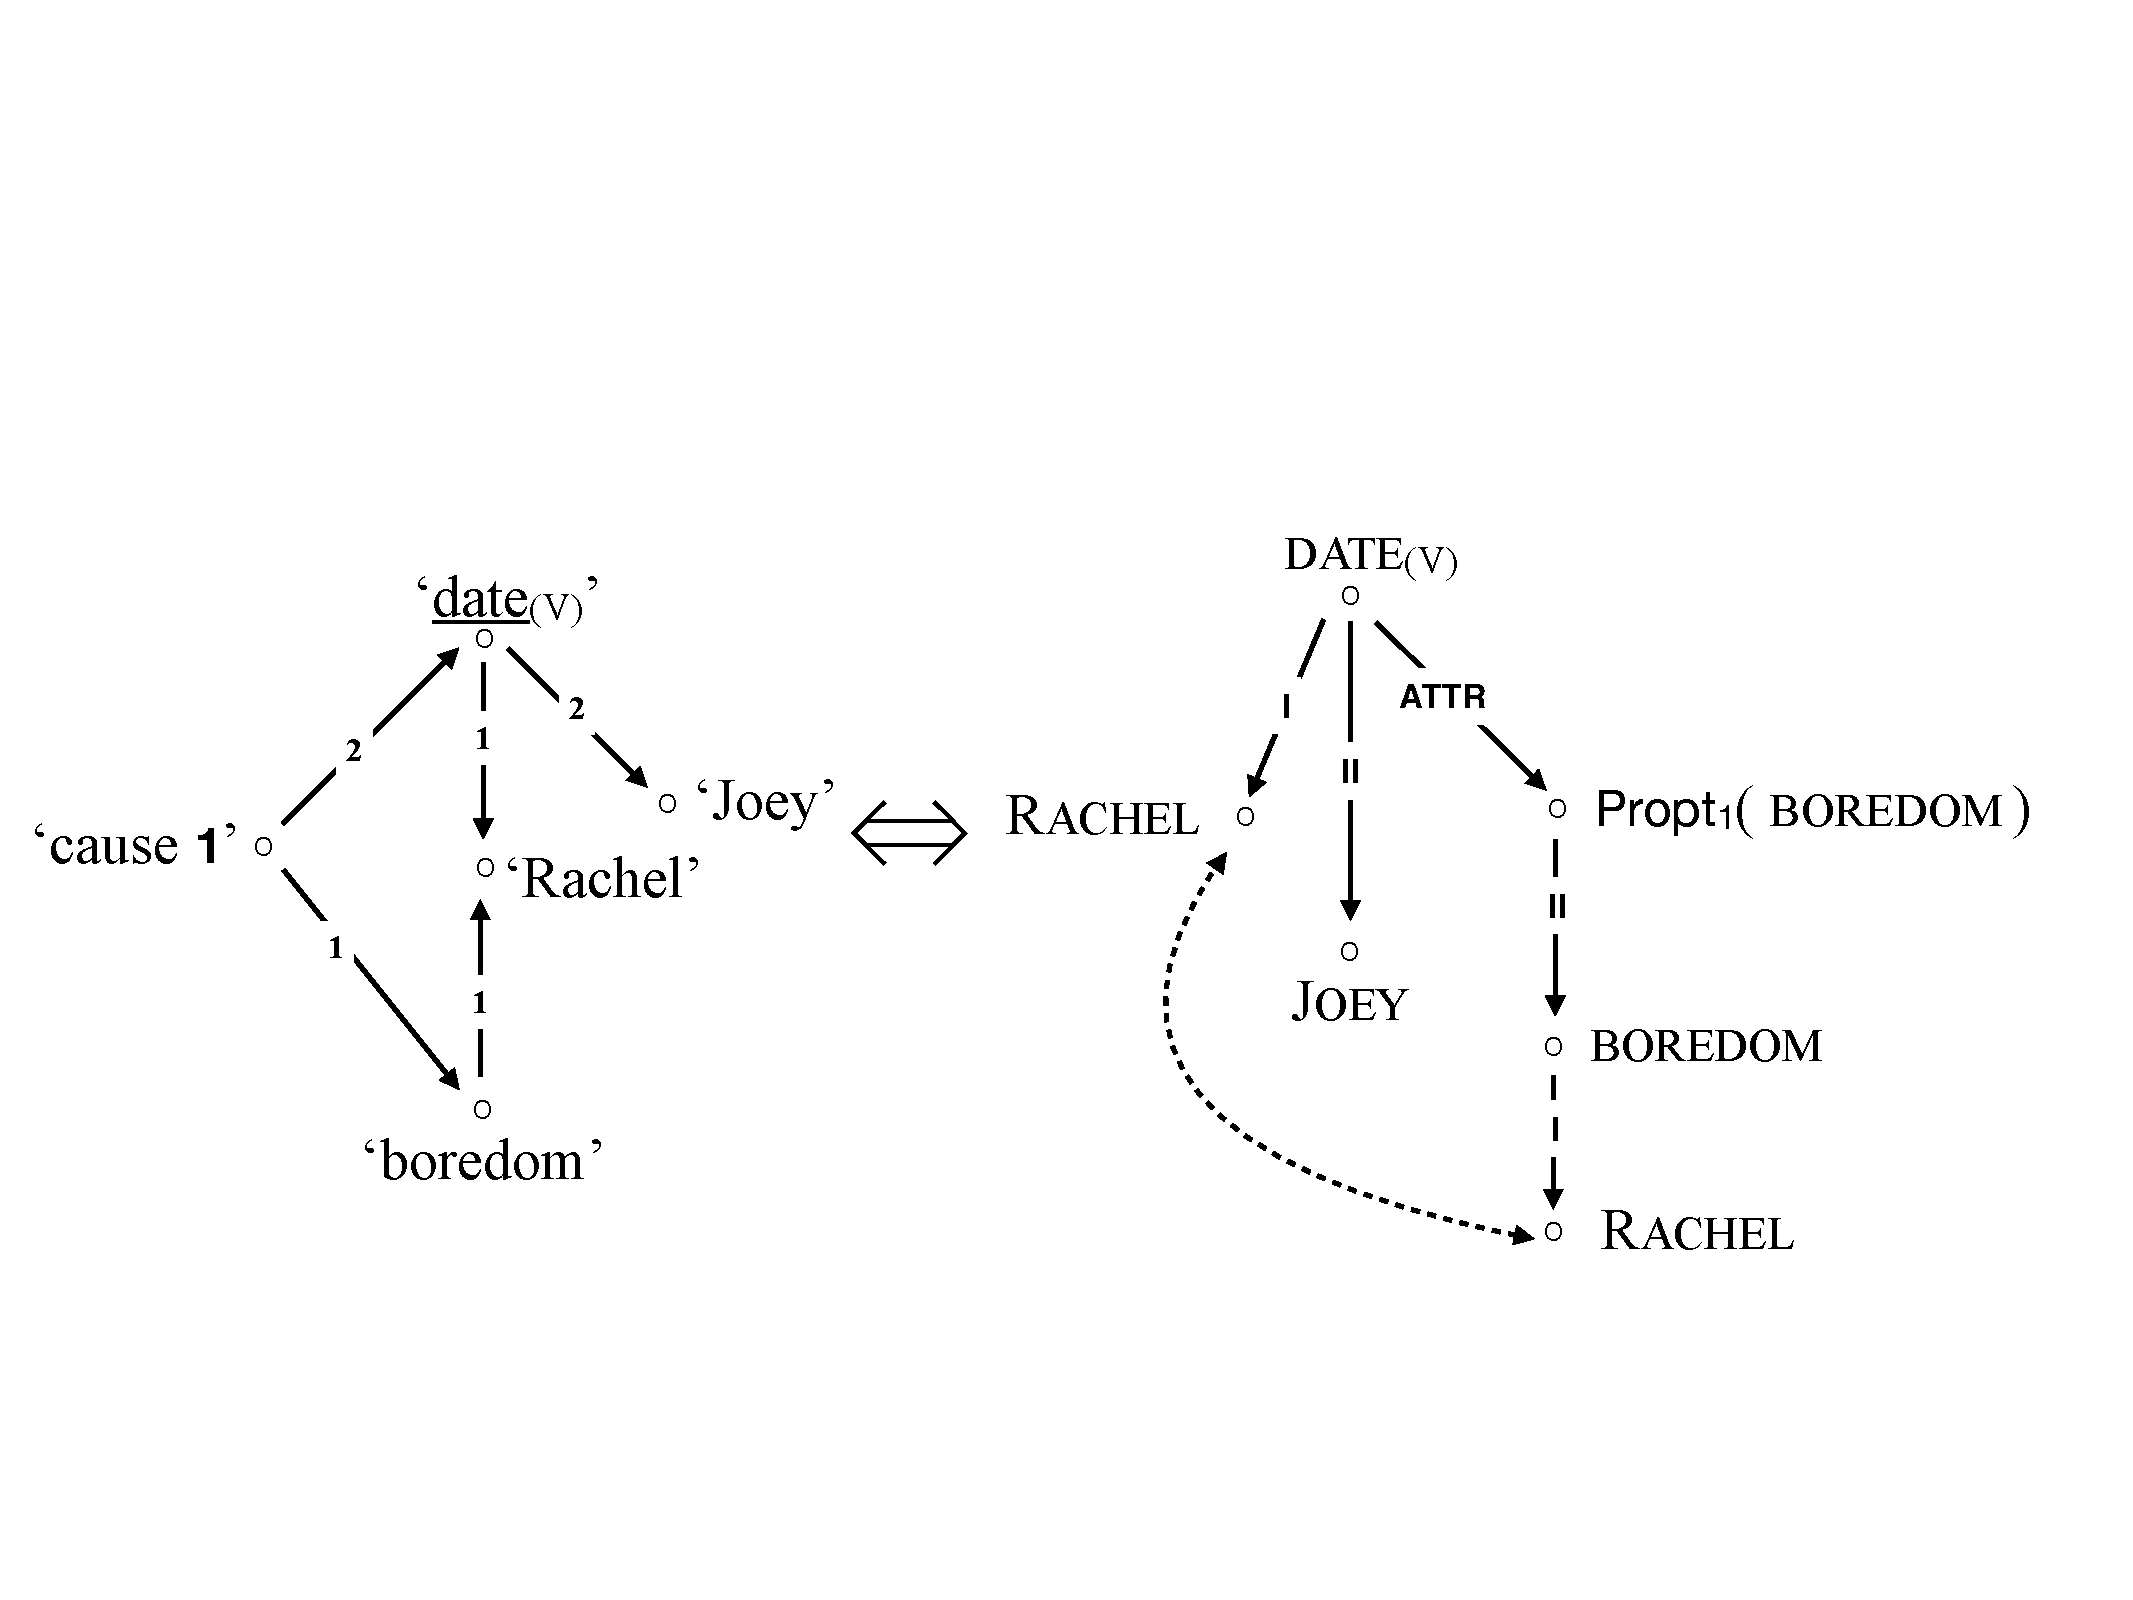
\includegraphics[width=11.5cm]{Fig/SyntLF/SemSyntPropt-i-illustr.pdf}
\caption[Illustration of \lf{Propt\tsub{1}} in the Sem\thinspace$\Leftrightarrow$\thinspace{}DSynt correspondence]{Illustration of \lf{Propt\tsub{1}} in the Sem\thinspace$\Leftrightarrow$\thinspace{}DSynt correspondence\footnotemark}\label{fig:Propt-i-illustr}
\end{figure}\footnotetext{On the non-agentive `cause\sensenum{1}' vs. the agentive `cause\sensenum{2}', see ``\nameref*{par:Cause1Cause2},'' p.\thinspace\pageref{par:Cause1Cause2}.}

Because of its meaning, \lf{Propt\tsub{i}} is naturally related to the LF \lf{Caus}\index[lf]{Caus@\lf{Caus}} (\sectref{sec:collocCausatif}, [\ref{lf:Caus}], p.\thinspace\pageref{lf:Caus}), such that it is possible to write the following deep-syntactic paraphrasing rule for \lf{Propt\tsub{1}}\index[lf]{Propti@\lf{Propt\tsub{i}}!\lf{Propt\tsub{1}}}:

\begin{center}
\phantomsection\label{txt:RParaphPropt1}\APolbox{11.6cm}{%
\textbf{R\tsub{\lf{Propt$_\text{1}$}}:} \\*
{L\tsub{(V)}\thinspace\syntRel{ATTR}\thinspace\lfappl{Propt\tsub{i}}{L}\syntRel{II}L\enskip{\small$\equiv$}\enskip{}L\thinspace\syntRelLeft{I}\thinspace\lfappl{CausFunc\tsub{0}}{\lfappl{S\tsub{0}}{L\tsub{(V)}}}\thinspace\syntRel{II}\thinspace\lfappl{S\tsub{0}}{L\tsub{(V)}}} \\*[3pt] 
\small
\begin{tabular}{p{10.8cm}}
\leftskip=0.5cm\textit{The bar closed for}\tsub{\lfappl{Propt$_\text{1}$}{\textit{lack}\tsub{(N)}}} \textit{lack of customers.} \\
\leftskip=0.5cm$\equiv$ \\
\leftskip=0.5cm\textit{The lack of customers lead}\tsub{\lfappl{CausFunc$_\text{0}$}{\lfappl{S$_\text{0}$}{\textit{close}\tsub{(V)}}}} \textit{to the closure}\tsub{\lfappl{S$_\text{0}$}{\textit{close}\tsub{(V)}}} \textit{of the bar.}
\end{tabular}
}
\end{center}\index[notion]{paraphrase!deep-syntactic paraphrasing rule!\textbf{R\tsub{\lf{Propt$_\text{1}$}}}|emph}

\begin{quote}
\begingroup
\small
\begin{tabular}{ l c }
   \midrule
   \multicolumn{2}{l}{\lf{Propt\tsub{i}}: adverbial} \\
   \midrule
   \textbf{L} & N \\
   \midrule
   \textbf{\lfappl{Propt\tsub{i}}{L}} & Adv \\
   \midrule
\end{tabular}
\endgroup
\end{quote}

\phantomsection\label{txt:Propt1UnderTheEffectOfAlcohol}\begin{longtable*}[l]{ l l >{\raggedright\arraybackslash}p{7cm} }

\multicolumn{3}{l}{\textbf{English}} \\*

\lfappl{Propt\tsub{1}}{\textit{interest}\tsub{(N)}} & = & \textit{out}\onewdf\textit{of} \lfgp{\textsc{art} \tld} \\
\lfappl{Propt\tsub{1}}{\textit{alcohol}} & = & \textit{under the effect} \lfgp{\textit{of} \tld}\textbf{;} \fused\idiom{\textit{under the influence}} \\
\lfappl{Propt\tsub{1}}{\textit{combat}\tsub{(N)}} & = & \textit{in} \lfgp{\tld} \\
\lfappl{Propt\tsub{1}}{\textit{\idiom{heart attack}}} & = & \textit{of} \lfgp{\textsc{(art)} \tld} \\
\lfappl{Propt\tsub{1}}{\textit{lack}\tsub{(N)}} & = & \textit{for} \lfgp{\tld} \\
\multicolumn{3}{l}{\quad\lfgp{N\tsub{X}\textit{'s lack of} N\tsub{Y}}} \\
\lfappl{Propt\tsub{2}}{\textit{attack}} & = & \textit{in} \lfgp{\textsc{art} \tld} \\[6pt]

\multicolumn{3}{l}{\textbf{French}} \\*

\lfappl{Propt\tsub{1}}{\textit{intérêt}} & = & \textit{par} \lfgp{\tld} \\
\lfappl{Propt\tsub{1}}{\textit{alcool}} & = & \textit{sous l'emprise} \lfgp{\textit{de} \textsc{art} \tld} \\
\lfappl{Propt\tsub{1}}{\textit{combat}} & = & \textit{à} \lfgp{\textit{le} \tld} \lfgp{$\Rightarrow$ \textit{au combat}} \\
\lfappl{Propt\tsub{1}}{\textit{\idiom{crise cardiaque}}} & = & \textit{de} \lfgp{\textsc{(art)} \tld} \\
\lfappl{Propt\tsub{2}}{\textit{manque}} & = & \textit{par} \lfgp{\tld} \\
\multicolumn{3}{l}{\quad\lfgp{\textit{manque de} N\tsub{X} \textit{pour} N\tsub{Y}}} \\
\lfappl{Propt\tsub{2}}{\textit{attentat}} & = & \textit{dans} \lfgp{\textsc{art} \tld} \\[6pt]

\multicolumn{3}{l}{\textbf{Russian}} \\*

\lfappl{Propt\tsub{1}}{\textit{interes}} & = & \textit{iz} \lfgp{\tld\textit{a}} \\
\lfappl{Propt\tsub{1}}{\textit{alkogol\suffixsplit{}\palati}} & = & \textit{pod vozdejstviem} \lfgp{\tld\textit{ja}} \\
\lfappl{Propt\tsub{1}}{\textit{boj}} & = & \textit{v}\sensenum{1} \lfgp{\tld\textit{u}} \\
\lfappl{Propt\tsub{1}}{\textit{infarkt}} & = & \textit{ot} \lfgp{\tld\textit{a}} \\
\lfappl{Propt\tsub{2}}{\textit{otsutstvi\suffixsplit{}e}} & = & \textit{iz-za} \lfgp{\tld\textit{ja}} \\
\multicolumn{3}{l}{\quad\lfgp{\textit{otsutstvie} N\tsub{X-GEN} \textit{u} N\tsub{Y-GEN}}} \\
\lfappl{Propt\tsub{2}}{\textit{pokušeni\suffixsplit{}e}} & = & \textit{v rezul\palati{}tate} \lfgp{\tld\textit{ja}} \\

\end{longtable*}

The syntagmatic LF \lf{Propt\tsub{1}}, which includes causation\index[notion]{causation}, should not be mistaken for the non-causative paradigmatic LF\index[notion]{lexical function!paradigmatic vs. syntagmatic \tlds} \lf{Adv\tsub{1}}\index[lf]{Advi@\lf{Adv\tsub{i}}};  cf. the following contrast:

\begingroup
\small

\ex. \begingroup\setlength{\tabcolsep}{2pt}
\begin{tabular}[t]{ l l >{\raggedright\arraybackslash}p{7cm} }
\lfappl{Adv\tsub{1}}{\textit{affection}} & = & \textit{affectionately}\textbf{,} \textit{with} \tld \\*
\multicolumn{3}{l}{vs.} \\*
\lfappl{Propt\tsub{1}}{\textit{affection}} & = & \textit{out}\onewdf\textit{of} \lfgp{\tld} \\
\end{tabular}\endgroup

\endgroup

See also, on \lf{Adv\tsub{i}}, \chapref{chap:paraLFs}, \sectref{sec:derivAdvAct}, [\ref{lf:Adv-i}], p.\thinspace\pageref{lf:Adv-i}. For a detailed study of \lf{Propt\tsub{i}}, see \textcite[503--617]{IordanskajaMelcuk2007}.\phantomsection\label{txt:endPropt-i}

\section{Verbal collocates}\label{sec:verbalCollocates}

\subsection{Copula verb}\label{sec:verbeCopule}\index[notion]{copula verb}\index[notion]{verb!copula \tld}

\refstepcounter{LFlist}
\subsubsection*{{\small [\arabic{LFlist}]} \lf{Copul} \lfgp{{\scriptsize Latin} \textit{copula}}: verb that means `be'}\label{lf:Copul}
\addcontentsline{toc}{subsection}{{\footnotesize [\arabic{LFlist}]} \lf{Copul}: verb that means `be'}\index[lf]{Copul@\lf{Copul}|emph}

\lfappl{Copul}{L} is a verb that means `be\tsub{(copula)}' and applies to a nominal or adjectival\slashs{}adverbial lexical unit L. It takes L as DSyntA\thinspace\syntDname{II}; its DSyntA\thinspace\syntDname{I} is the DSyntA\thinspace\syntDname{I} of L.

\begin{quote}
\begingroup
\small
\begin{tabular}{ l c c c }
   \midrule
   \multicolumn{4}{l}{\lf{Copul}: verbal} \\
   \midrule
   \textbf{L} & N & Adj & Adv \\
   \midrule
   \textbf{\lfappl{Copul}{L}} & V & V & V \\
   \midrule
\end{tabular}
\endgroup
\end{quote}

\begin{longtable*}[l]{ l l >{\raggedright\arraybackslash}p{6cm} }

\multicolumn{3}{l}{\textbf{English}} \\*

\lfappl{Copul}{\textit{example}} & = & \textit{be} \lfgp{\textsc{art} \tld}\textbf{,} \textit{serve} \lfgp{\textit{as an} \tld} \\
\lfappl{Copul}{\textit{challenge}\tsub{(N)}} & = & \textit{be}\textbf{,} \textit{constitute}\textbf{,} \textit{represent} \lfgp{\textsc{art} \tld} \\
\lfappl{Copul}{\textit{true}} & = & \textit{be}\textbf{,} \textit{hold} \lfgp{\tld} \\
\lfappl{IncepCopul}{\textit{dead}\tsub{(Adj)}} & = & \textit{drop} \lfgp{\tld} \\[6pt]

\multicolumn{3}{l}{\textbf{French}} \\*

\lfappl{Copul}{\textit{exemple}} & = & \textit{être} \lfgp{\textsc{art} \tld}\textbf{,} \textit{servir} \lfgp{\textit{d'}\tld} \\
\lfappl{Copul}{\textit{défi}} & = & \textit{être}\textbf{,} \textit{constituer}\textbf{,} \textit{représenter} \lfgp{\textsc{art} \tld} \\
\lfappl{IncepCopul}{\textit{amoureux}\tsub{(Adj)}} & = & \textit{tomber} \lfgp{\tld} \\[6pt]

\multicolumn{3}{l}{\textbf{Russian}} \\*

\lfappl{Copul}{\textit{primer}} & = & \textit{byt\palati}\textbf{,} \textit{slu\v{z}it\palati} \lfgp{\tld\textit{om}} \\
\lfappl{IncepCopul}{\textit{zamertvo}} & = & \textit{upast\palati} \lfgp{\tld} \\
\lfappl{IncepCopul}{\textit{vljublënnyj}} & = & \fused\textit{vljubit\palati{}sja} \\

\end{longtable*}

\lf{Copul} is an analytic\index[notion]{derivative!analytic semantic \tld} variant of the paradigmatic LF \lf{Pred}\index[lf]{Pred@\lf{Pred}}\index[notion]{lexical function!paradigmatic vs. syntagmatic \tlds} (\chapref{chap:paraLFs}, [\ref{lf:Pred}], p.\thinspace\pageref{lf:Pred}), so that the following equivalence holds: \lfappl{Copul}{L}\thinspace\syntRel{II}\thinspace{}L\enskip{\small$\equiv$}\enskip\lfappl{Pred}{L}. For instance:

\begingroup
\small

\ex. Her declaration was\tsub{\lfappl{Copul}{\textit{unexpected}}} unexpected.\\
     $\equiv$ \\
     Her declaration \idiom{came as a bolt from the blue}\tsub{\lfappl{Pred}{\textit{unexpected}}}.

\endgroup

\lf{Copul} does not have many values in any given natural language. It is mainly used within complex LFs, as in \lf{IncepCopul}\index[lf]{Incep@\lf{Incep}}, etc.

%\lfappl{Copul}{L} can be semantically (quasi-)equivalent to \lfappl{Oper\tsub{1}}{L} (Sec.~\ref{sec:verbeSupport} below, [\ref{lf:Oper-i}], p.\thinspace\pageref{lf:Oper-i}) if L is an Adj\slashs{}Adv or a quasi-predicative N semantically close to an Adj (\textsc{idiot}\tsub{(N)}, \textsc{genius}, etc.).

\subsection{Support [=~light] verbs}\label{sec:verbeSupport}\index[notion]{support verb|emph}\index[notion]{verb!support \tld|emph}

All LFs \lf{f} introduced in this section are ``pure'' verbalizers\index[notion]{verbalizer}. They are such that:

\begin{itemize}

\item \lf{f} applies to a non-verbal lexical unit L, and \lfappl{f}{L} takes L as DSyntA\thinspace\syntDname{I} (i.e., subject)\index[notion]{subject, syntactic} or DSyntA\thinspace\syntDname{II}\slashs\syntDname{III}\slashs... (i.e., object)\index[notion]{object, syntactic};

\item \lfappl{f}{L} is not selected by the Speaker\index[notion]{Speaker, the} to express a given meaning, but in order to construct a well-formed verbal syntactic structure with the same meaning as L.

\end{itemize}

Each \lfappl{f}{L} of this type, so to speak, ``supports'' a non-verbal L, by enabling the collocation \lfappl{f}{L}\thinspace$\rightarrow$\thinspace{}L to function as the syntactic head of the clause; hence the term \notion{support verb} \parencite{GrossM1981}. Because support verbs are semantically ``light,'' i.e. they do not semantically contribute to the sentence, they are also referred to as \notion{light verbs}\index[notion]{light verb|see{support verb}}\index[notion]{verb!light \tld|see{support verb}}, a term generally attributed to \textcite[Ch.~VII, \S\thinspace7.2{\footnotesize 1--5}]{Jespersen1946}.%\footnote{For a comparison between the notion of support verb and the closely related notion of \textit{Funktionsverb} in German studies, see \textcite{Langer2005}.}

\begin{soundboxnotitle}
A support verb is semantically empty in the collocation it forms with L in actual utterances. But this does not prevent it from having an inherent meaning in the lexicon\index[notion]{lexicon}, this meaning becoming redundant with respect  to that of L. Such is the case, for instance, of the verb \textsc{feel}\tsub{(V)} in the collocation \textit{feel pain}, the verb \textsc{face}\tsub{(V)} in \textit{face an ultimatum}, etc.
\end{soundboxnotitle}

There are three types of support verbs according to the position of the collocation base L in their DSynt-actantial structure: \lf{Oper\tsub{i}}, \lf{Func\tsub{i}} and \lf{Labor\tsub{ij}}. These three LFs have the same PoS table:

\begin{quote}
\begingroup
\phantomsection\label{tab:PdDVSup}\small
\begin{tabular}{ l c c c }
   \midrule
   \multicolumn{4}{l}{\lf{Oper\tsub{i}}, \lf{Func\tsub{i}}, \lf{Labor\tsub{ij}}: verbal} \\
   \midrule
   \textbf{L} & N & Adj & Adv \\
   \midrule
   \textbf{\lfappl{Oper\tsub{i}\slashs{}Func\tsub{i}\slashs{}Labor\tsub{ij}}{L}} &V & V & V \\
   \midrule
\end{tabular}
\endgroup
\end{quote}

A typical support verb collocation is controlled by a nominal base; almost all examples that follow present this type of collocation. However, adjectival and adverbial bases for such collocations are limitedly possible; a few illustrations are provided at the end of this section.

A support verb LF, being empty by definition, cannot be semantically characterized. We will, thus, supply for each LF described below -- \lf{Oper\tsub{i}}, \lf{Func\tsub{i}} and \lf{Labor\tsub{ij}} -- a prototypical lexical equivalent, so that the reader can have an intuitive feeling of its usage (cf. \textsc{do}\tsub{(V)} for \lf{Oper\tsub{i}}).

\refstepcounter{LFlist}
\subsubsection*{{\small [\arabic{LFlist}]} \lf{Oper\tsub{i}} \lfgp{{\scriptsize Latin} \textit{oper\={a}ri} `do, carry out'}: support verb analogous to \textsc{do}\tsub{(V)}\label{lf:Oper-i}}
\addcontentsline{toc}{subsection}{{\footnotesize [\arabic{LFlist}]} \lf{Oper\tsub{i}}: support verb analogous to \textsc{do}\tsub{(V)}}\index[lf]{Operi@\lf{Oper\tsub{i}}|emph}

\lfappl{Oper\tsub{i}}{L} is a support verb that takes L as DSyntA\thinspace\syntDname{II} and the DSyntA\thinspace\syntDname{i} of L as DSyntA\thinspace\syntDname{I}.

\lf{Oper\tsub{i}} participates in the Sem\thinspace$\Leftrightarrow$\thinspace{}DSynt\index[notion]{structure!semantic \tld\ [SemS]}\index[notion]{semantic!\tld\ structure [SemS]}\index[notion]{structure!deep-syntactic \tld\ [DSyntS]}\index[notion]{deep-syntactic!\tld\ structure [DSyntS]} correspondence\index[notion]{correspondence between representation levels} shown in \figref{fig:Oper-i}.

\begin{figure}
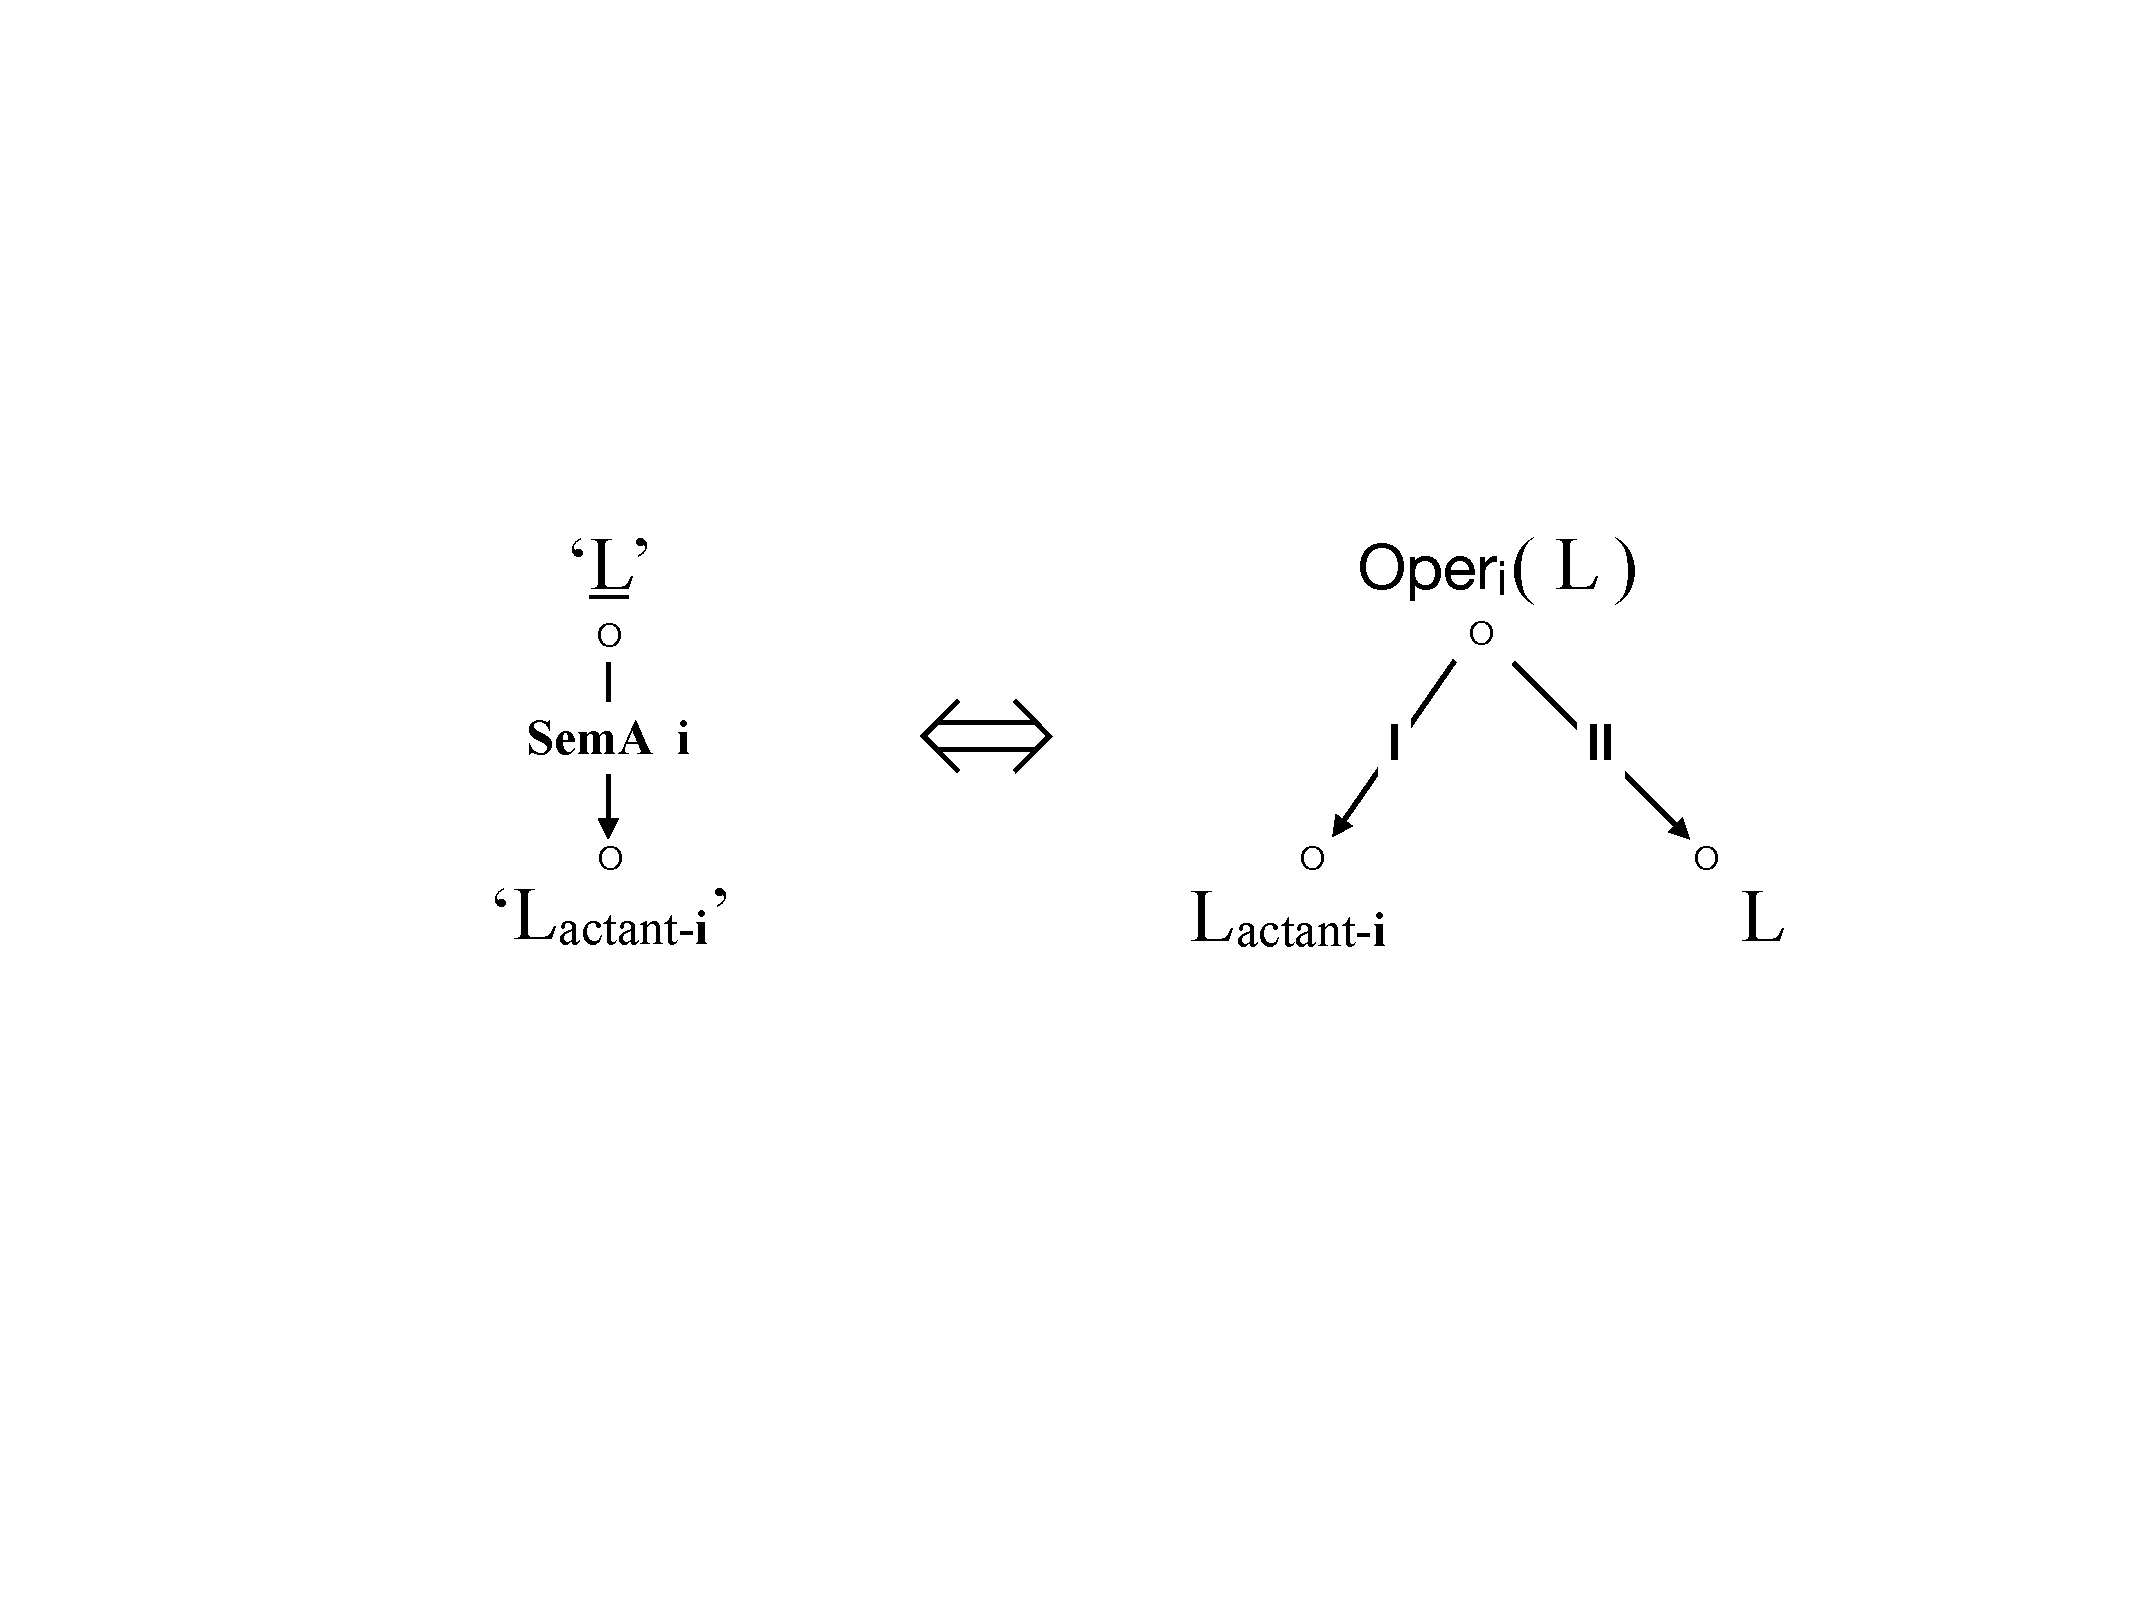
\includegraphics[height=22mm]{Fig/SyntLF/SemSyntOper-i.pdf}
\caption{\lf{Oper\tsub{i}} in the Sem\thinspace$\Leftrightarrow$\thinspace{}DSynt correspondence}\label{fig:Oper-i}
\end{figure}

\figref{fig:Oper-i-illustr} illustrates the correspondence template in \figref{fig:Oper-i} for \lf{Oper\tsub{1}}\index[lf]{Operi@\lf{Oper\tsub{i}}!\lf{Oper\tsub{1}}} with L~=~\textsc{fever}.

\begin{figure}
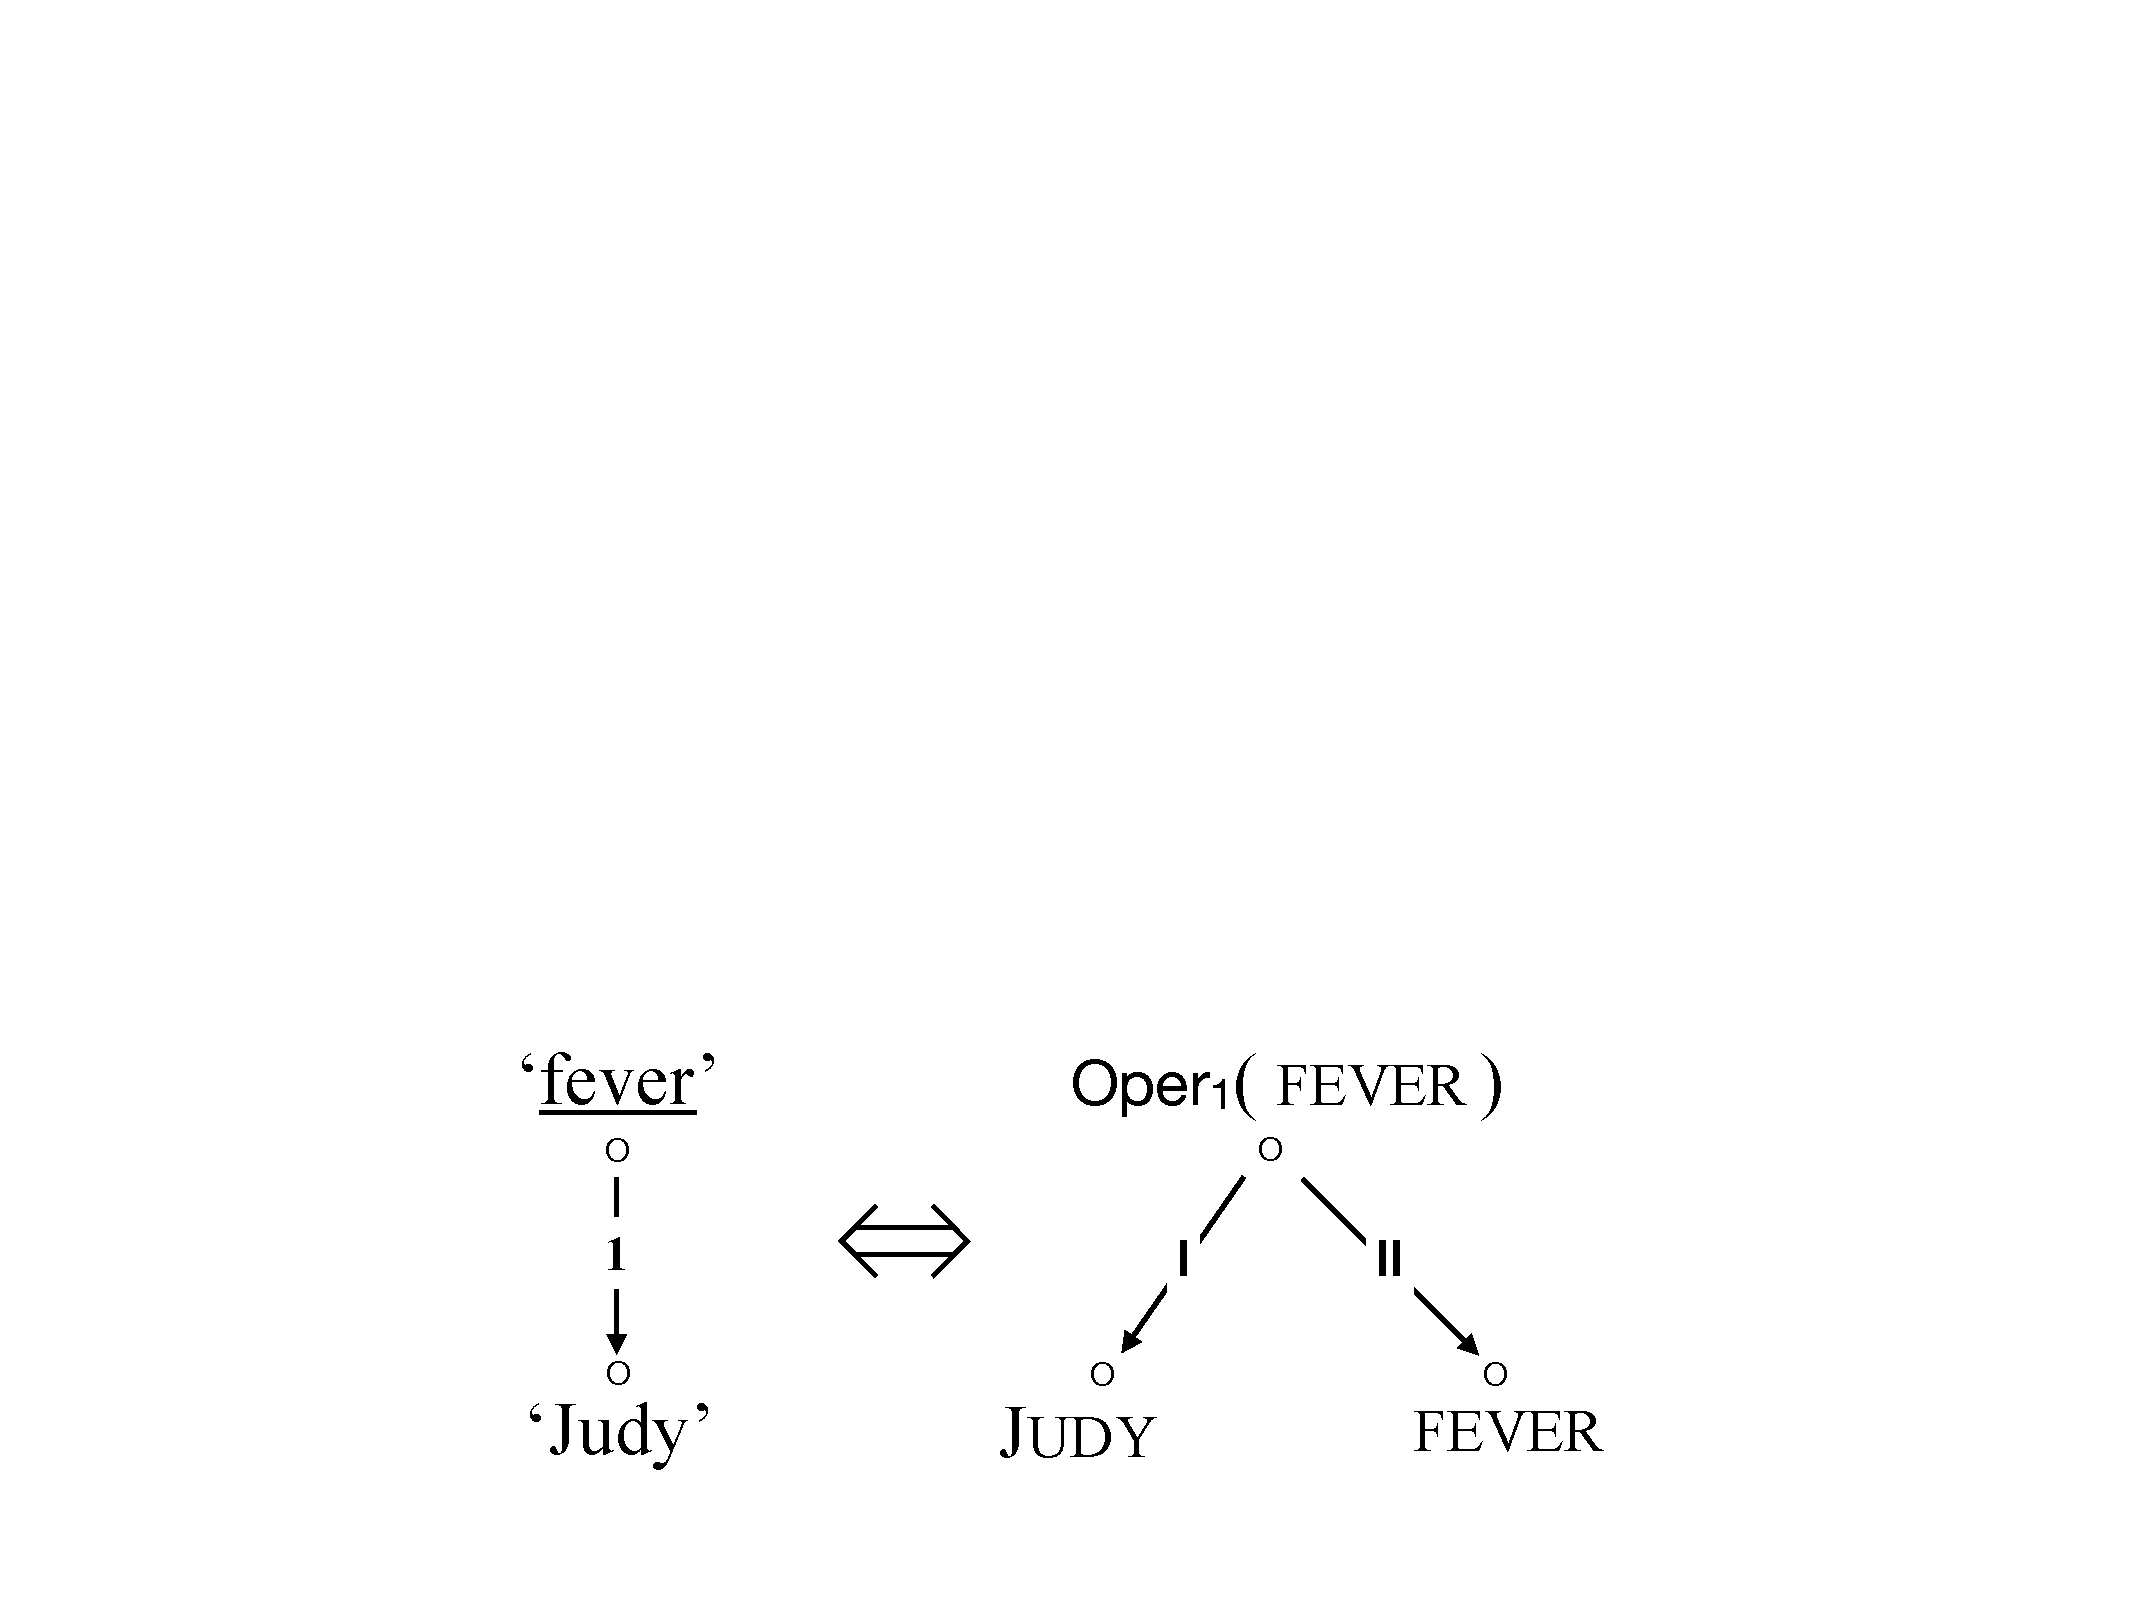
\includegraphics[height=22mm]{Fig/SyntLF/SemSyntOper-i-illustr.pdf}
\caption{\lf{Oper\tsub{1}} in the Sem\thinspace$\Leftrightarrow$\thinspace{}DSynt correspondence with L~=~\textsc{fever}}\label{fig:Oper-i-illustr}
\end{figure}

Sentences \Next[a--b] are possible implementations of the DSynt-structure given in \figref{fig:Oper-i-illustr}:

\begingroup
\small

\ex. \a. Judy \emph{has} a fever.
     \b. Judy \emph{runs} a fever.

\endgroup

\lfappl{Oper\tsub{i}}{L} can be an impersonal\index[notion]{verb!impersonal \tld}\index[notion]{impersonal verb} support verb, which has no DSyntA\thinspace\syntDname{I}. In such a case, the notation \lfappl{Oper\tsub{0}}{L}\index[lf]{Operi@\lf{Oper\tsub{i}}!\lf{Oper\tsub{0}}|emph} is used (see French and Russian illustrations below).

\begin{longtable*}[l]{ l l >{\raggedright\arraybackslash}p{6cm} }

\multicolumn{3}{l}{\textbf{English}} \\*

\lfappl{Oper\tsub{1}}{\textit{crime}} & = & \textit{commit}\textbf{,} \textit{perpetrate} \lfgp{\textsc{art} \tld} \\
\lfappl{Oper\tsub{1}}{\textit{supremacy}} & = & \textit{detain} \lfgp{\textsc{art} \tld} \\
\lfappl{Oper\tsub{2}}{\textit{bullying}} & = & \textit{undergo} \lfgp{\tld} \\
\lfappl{Oper\tsub{2}}{\textit{danger}} & = &  \textit{run} \lfgp{\textsc{art} \tld} \\
\lfappl{Oper\tsub{2}}{\textit{applause}} & = & \textit{draw}\textbf{,} \textit{get}\textbf{,} \textit{win} \lfgp{\tld\ \lfconstr{with a modifier}} \\
\lfappl{Oper\tsub{3}}{\textit{order}\tsub{(N)}} & = & \textit{get}\textbf{,} \textit{receive} \lfgp{\textsc{art} \tld} \\
\multicolumn{3}{l}{\quad\lfgp{N\tsub{X}\textit{'s order to} V\tsub{Y} \textit{to} N\tsub{Z}}} \\
\lfappl{Oper\tsub{3}}{\textit{refusal}} & = & \textit{meet} \lfgp{\textit{with} \textsc{(art)} \tld} \\
\multicolumn{3}{l}{\quad\lfgp{N\tsub{X}\textit{'s refusal to} V\tsub{Y} \textit{to} N\tsub{Z}}} \\[6pt]

\multicolumn{3}{l}{\textbf{French}} \\*

\lfappl{Oper\tsub{0}}{\textit{nuit}} & = & \lfgp{\textit{il}\tsub{(impers)}} \textit{faire} \lfgp{\tld}\\
\lfappl{Oper\tsub{0}}{\textit{soif}} & = & \uslabel{informal} \lfgp{\textit{il}\tsub{(impers)}} \textit{faire} \lfgp{\tld}\\
\lfappl{Oper\tsub{1}}{\textit{méfait}} & = & \textit{perpétrer} \lfgp{\textsc{art} \tld}\\
\lfappl{Oper\tsub{1}}{\textit{suprématie}} & = & \textit{détenir} \lfgp{\textsc{art} \tld}\\
\lfappl{Oper\tsub{2}}{\textit{calomnie}} & = & \textit{subir} \lfgp{\textsc{art} \tld}\\
\lfappl{Oper\tsub{2}}{\textit{danger}} & = & \textit{courir} \lfgp{\textsc{art} \tld}\\
\lfappl{Oper\tsub{2}}{\textit{applaudissements}} & = & \textit{recueillir} \lfgp{\textsc{art} \tld}\\
\lfappl{Oper\tsub{3}}{\textit{consensus}} & = & \textit{faire} \lfgp{\tld}\\
\multicolumn{3}{l}{\quad\lfgp{\textit{concensus entre} N\tsub{X} \textit{et} N\tsub{Y} \textit{à propos de} N\tsub{Z}}} \\
\lfappl{Oper\tsub{3}}{\textit{refus}} & = & \textit{essuyer} \lfgp{\textsc{art} \tld}\textbf{,} \textit{se heurter} \lfgp{\textit{à} \textsc{art} \tld} \\*
\multicolumn{3}{l}{\quad\lfgp{\textit{refus de} N\tsub{X} \textit{de} V\tsub{Y-\textsc{inf}} \textit{à} N\tsub{Z}}} \\[6pt]

\multicolumn{3}{l}{\textbf{Russian}} \\*

\lfappl{Oper\tsub{0}}{\textit{zapax}} & = &  \textit{tjanut\palati} \lfgp{\tld\textit{om}} \\
\lfappl{Oper\tsub{0}}{\textit{proxlad\suffixsplit{}a}} & = &  \textit{vejat\palati} \lfgp{\tld\textit{oj}}  \\
\lfappl{Oper\tsub{1}}{\textit{prestupleni\suffixsplit{}e}} & = & \textit{sover\v{s}it\palati} \lfgp{\tld\textit{e}} \\
\lfappl{Oper\tsub{1}}{\textit{prevosxodstv\suffixsplit{}o}} & = & \textit{imet\palati} \lfgp{\tld\textit{o}} \\
\lfappl{Oper\tsub{2}}{\textit{izdevatel\palati{}stv\suffixsplit{}a}} & = & \textit{podvergat\palati{}sja} \lfgp{\tld\textit{am}} \\
\lfappl{Oper\tsub{2}}{\textit{opasnost\suffixsplit{}\palati}} & = &  \textit{podvergat\palati{}sja} \lfgp{\tld\textit{i}} \\
\lfappl{Oper\tsub{2}}{\textit{aplodisment\suffixsplit{}y}} & = & \textit{byt\palati\ vstre\v{c}en} \lfgp{\tld\textit{ami}} \\
\lfappl{Oper\tsub{3}}{\textit{prikaz}} & = & \textit{polu\v{c}it\palati} \lfgp{\tld} \\
\multicolumn{3}{l}{\quad\lfgp{\textit{prikaz} N\tsub{X-\textsc{gen}} N\tsub{Z-\textsc{dat}} V\tsub{Y-\textsc{inf}}}} \\
\lfappl{Oper\tsub{3}}{\textit{otkaz}} & = & \textit{natolknut\palati{}sja} \lfgp{\textit{na}\sensenum{2} \tld}\textbf{,} \textit{polu\v{c}it\palati} \lfgp{\tld} \\*
\multicolumn{3}{l}{\quad\lfgp{\textit{otkaz} N\tsub{X-\textsc{gen}} N\tsub{Z-\textsc{dat}} V\tsub{Y-\textsc{inf}}}} \\

\end{longtable*}

\lf{Oper\tsub{i}} is the most frequent among support verbs. This is explained by the following fact: the base of an \lf{Oper\tsub{i}} collocation is in most cases the direct object\index[notion]{object, syntactic!direct \tld} of the verb, and semantic constraints are the strongest between a transitive verb\index[notion]{verb!transitive \tld} and its direct object -- stronger than between a verb and its other actants. It is for this reason that natural languages phraseologize in the first place phrases of the form V\thinspace\syntRel{DirO}\thinspace{}N.

Understandably, \lf{Oper\tsub{i}} has the pride of place in paraphrasing\index[notion]{paraphrase} systems of natural languages, as illustrated by the following two cases.

\begin{enumerate}

\item \lfappl{Oper\tsub{1}}{\lfappl{S\tsub{0}}{L\tsub{(V)}}}\thinspace\syntRel{II}\thinspace\lfappl{S\tsub{0}}{L\tsub{(V)}} is a paraphrase of L\tsub{(V)}:
            
\begingroup
\small

\ex. Joey joked.\\*
     $\equiv$ \\*
     Joey cracked a joke.

\endgroup

On such equivalence, see syntactic paraphrasing rule \textbf{R\tsub{\lf{Oper$_\text{1}$}}}\index[notion]{paraphrase!deep-syntactic paraphrasing rule!\textbf{R\tsub{\lf{Oper$_\text{1}$}}}}, introduced in \chapref{chap:NotionLF}, \sectref{sec:LFStandardParaphrasing} (p.\thinspace\pageref{txt:RParaphOper1}).

\item \lf{Oper\tsub{2}} is in the same paraphrastic relation -- i.e., syntactic conversion\index[notion]{conversive} -- with \lf{Oper\tsub{1}} as found between the passive and the active voice\index[notion]{voice, grammatical} of a verb, cf. \Next[a--b]:

\begingroup
\small

\ex. \a. Rachel gave\tsub{\lf{Oper\tsub{1}}} a kiss to Joey.\\*
         $\equiv$ \\*
         Rachel kissed\tsub{active voice} Joey.\vspace{2pt}
     \b. Joey got\tsub{\lf{Oper\tsub{2}}} a kiss from Rachel.\\*
         $\equiv$ \\*
         Joey was kissed\tsub{passive voice} by Rachel.

\endgroup

\end{enumerate}

\paragraph*{Transfer of L's actants to support verbs.}\label{par:transferOfLsActants}

In collocations \lfappl{Oper\tsub{i}}{L}\thinspace\syntRel{II}\thinspace{}L\index[notion]{object, syntactic!direct \tld}, the DSyntAs of L can migrate -- i.e., be transferred under paraphrasing -- to \lfappl{Oper\tsub{i}}{L}. In other words, \lfappl{Oper\tsub{i}}{L} can host, besides its own two obligatory DSyntAs, additional \mbox{DSyntAs} coming from L. This transfer of actants\index[notion]{actant!transfer of deep-syntactic \tld} is known as (\notion{syntactic}) \notion{raising}\index[notion]{raising, syntactic} -- see \chapref{chap:preliminaryNotions}, \sectref{sec:syntacticNotions}, p.\thinspace\pageref{def:DSyntA}. It is illustrated in \ref{ex:Oper1-CRIME} with \lfappl{Oper\tsub{1}}{\textit{crime}}.\footnote{The two utterances in \ref{ex:Oper1-CRIME} are semantically quasi-equivalent: they express the same propositional meaning, but have different communicative organizations.}\index[notion]{communicative!\tld\ structure}\index[notion]{structure!communicative \tld}

\begingroup
\small

\ex.\label{ex:Oper1-CRIME} Joey committed\tsub{\lf{Oper\tsub{1}}} a terrible crime\thinspace\syntRel{II}\thinspace{}\emph{against decency}.\\*
     $\cong$ \\*
     a terrible crime that Joey committed\thinspace\syntRel{III}\thinspace{}\emph{against decency}

\endgroup

The transfer of actants from the collocation base to the verbal collocate may be performed for all types of support verbs LFs -- \lf{Oper\tsub{i}}, \lf{Func\tsub{i}} and \lf{Labor\tsub{ij}}, as well as for corresponding complex LFs (for instance, \lf{CausFunc\tsub{0}}).

\begin{furtherreading}
On support\slashs light verbs\index[notion]{support verb}\index[notion]{verb!support \tld}, see \textcite{GrossM1981}, \textcite{Melcuk2022b} and \textcite{FleischhauerRiccio2025}; on transfer of actants from a collocation base to the collocative verb, see \textcites[253--272]{AlonsoRamos2004}{AlonsoRamos2007}.
\end{furtherreading}

\refstepcounter{LFlist}
\subsubsection*{{\small [\arabic{LFlist}]} \lf{Func\tsub{i}} \lfgp{{\scriptsize Latin} *\textit{function\={a}re} `[to] function'}: support verb analogous to\newline \idiom{\textsc{take place}}}\label{lf:Func-i}
\addcontentsline{toc}{subsection}{{\footnotesize [\arabic{LFlist}]} \lf{Func\tsub{i}}: support verb analogous to \idiom{\textsc{take place}}}\index[lf]{Funci@\lf{Func\tsub{i}}|emph}

\lfappl{Func\tsub{i}}{L} is a support verb that takes L as DSyntA\thinspace\syntDname{I} and the DSyntA\thinspace\syntDname{i} of L as DSyntA\thinspace\syntDname{II}. However, it can also have only one actantial dependent\index[notion]{dependent, syntactic}: L as DSynt\thinspace\syntDname{I}. In such a case -- an absolutely intransitive construction -- the LF is denoted as \lf{Func\tsub{0}}\index[lf]{Funci@\lf{Func\tsub{i}}!\lf{Func\tsub{0}}|emph}.

\lf{Func\tsub{i}} participates in the Sem\thinspace$\Leftrightarrow$\thinspace{}DSynt\index[notion]{structure!semantic \tld\ [SemS]}\index[notion]{semantic!\tld\ structure [SemS]}\index[notion]{structure!deep-syntactic \tld\ [DSyntS]}\index[notion]{deep-syntactic!\tld\ structure [DSyntS]} correspondence\index[notion]{correspondence between representation levels} shown in \figref{fig:Func-i}; it is to be compared to the \lfappl{Oper\tsub{i}}{L}\index[lf]{Operi@\lf{Oper\tsub{i}}} correspondence in \figref{fig:Oper-i} (p.\thinspace\pageref{fig:Oper-i}).

\begin{figure}
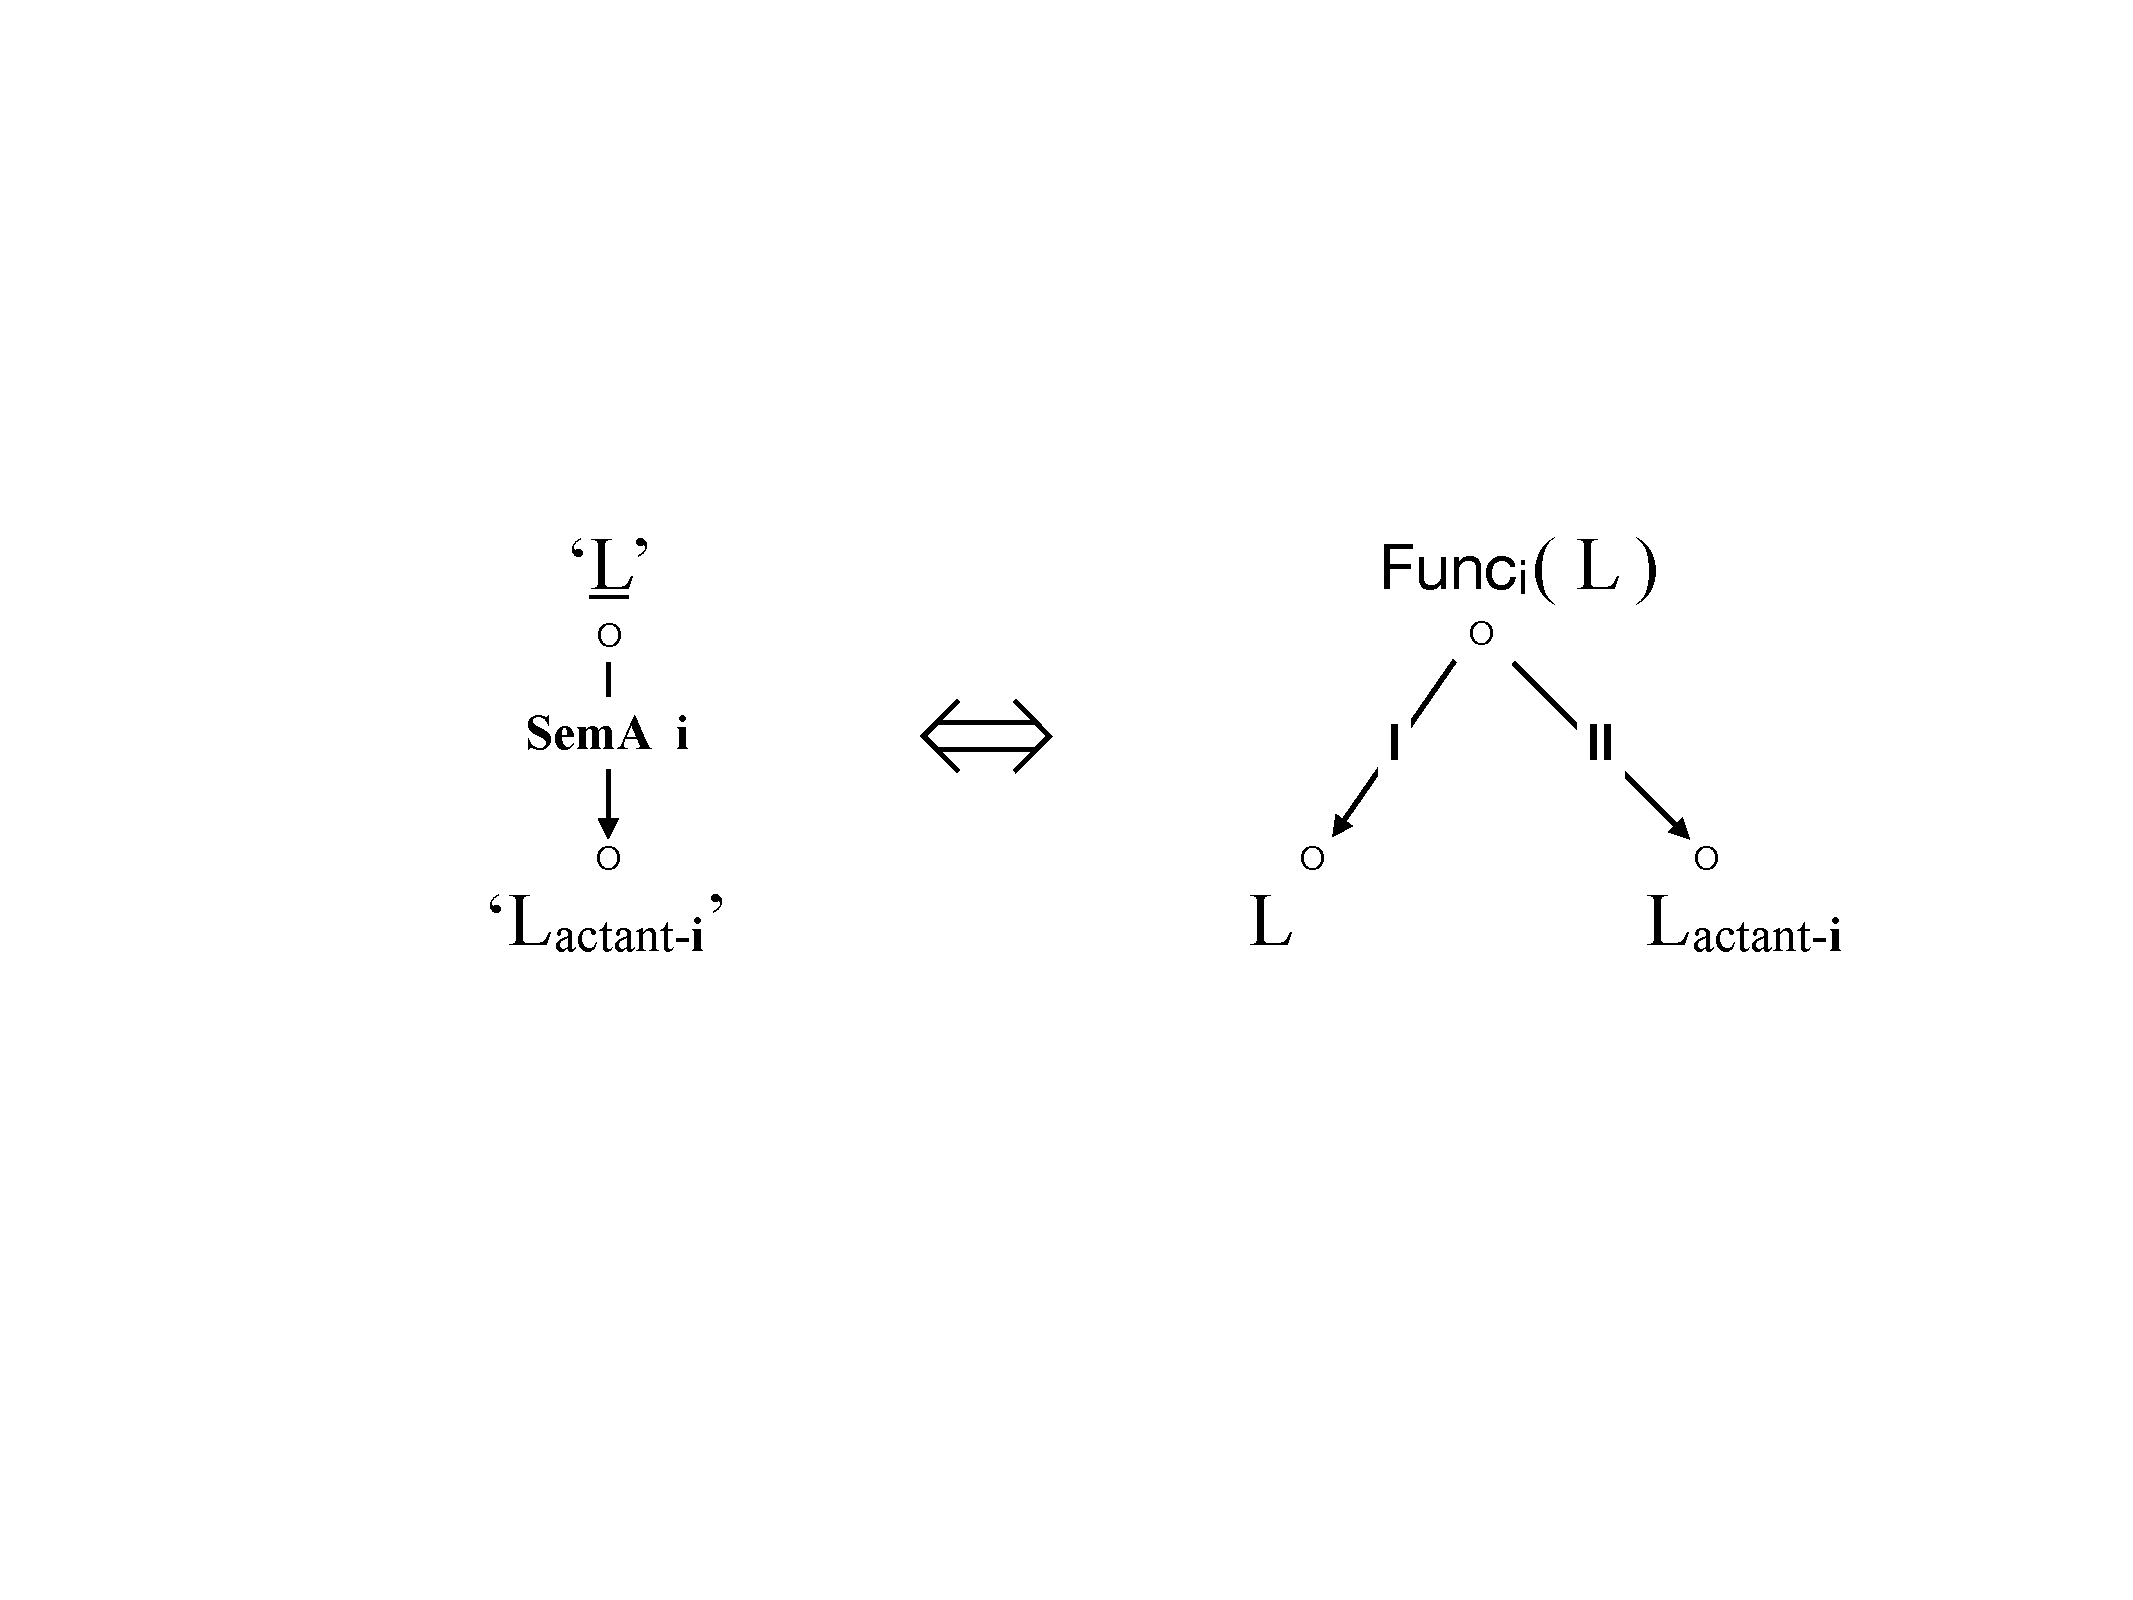
\includegraphics[height=22mm]{Fig/SyntLF/SemSyntFunc-i.pdf}
\caption{\lf{Func\tsub{i}} in the Sem\thinspace$\Leftrightarrow$\thinspace{}DSynt correspondence}\label{fig:Func-i}
\end{figure}

\figref{fig:Func-i-illustr} illustrates the correspondence template in \figref{fig:Func-i} for \lf{Func\tsub{1}} with L~= \textsc{responsibility}.

\begin{figure}
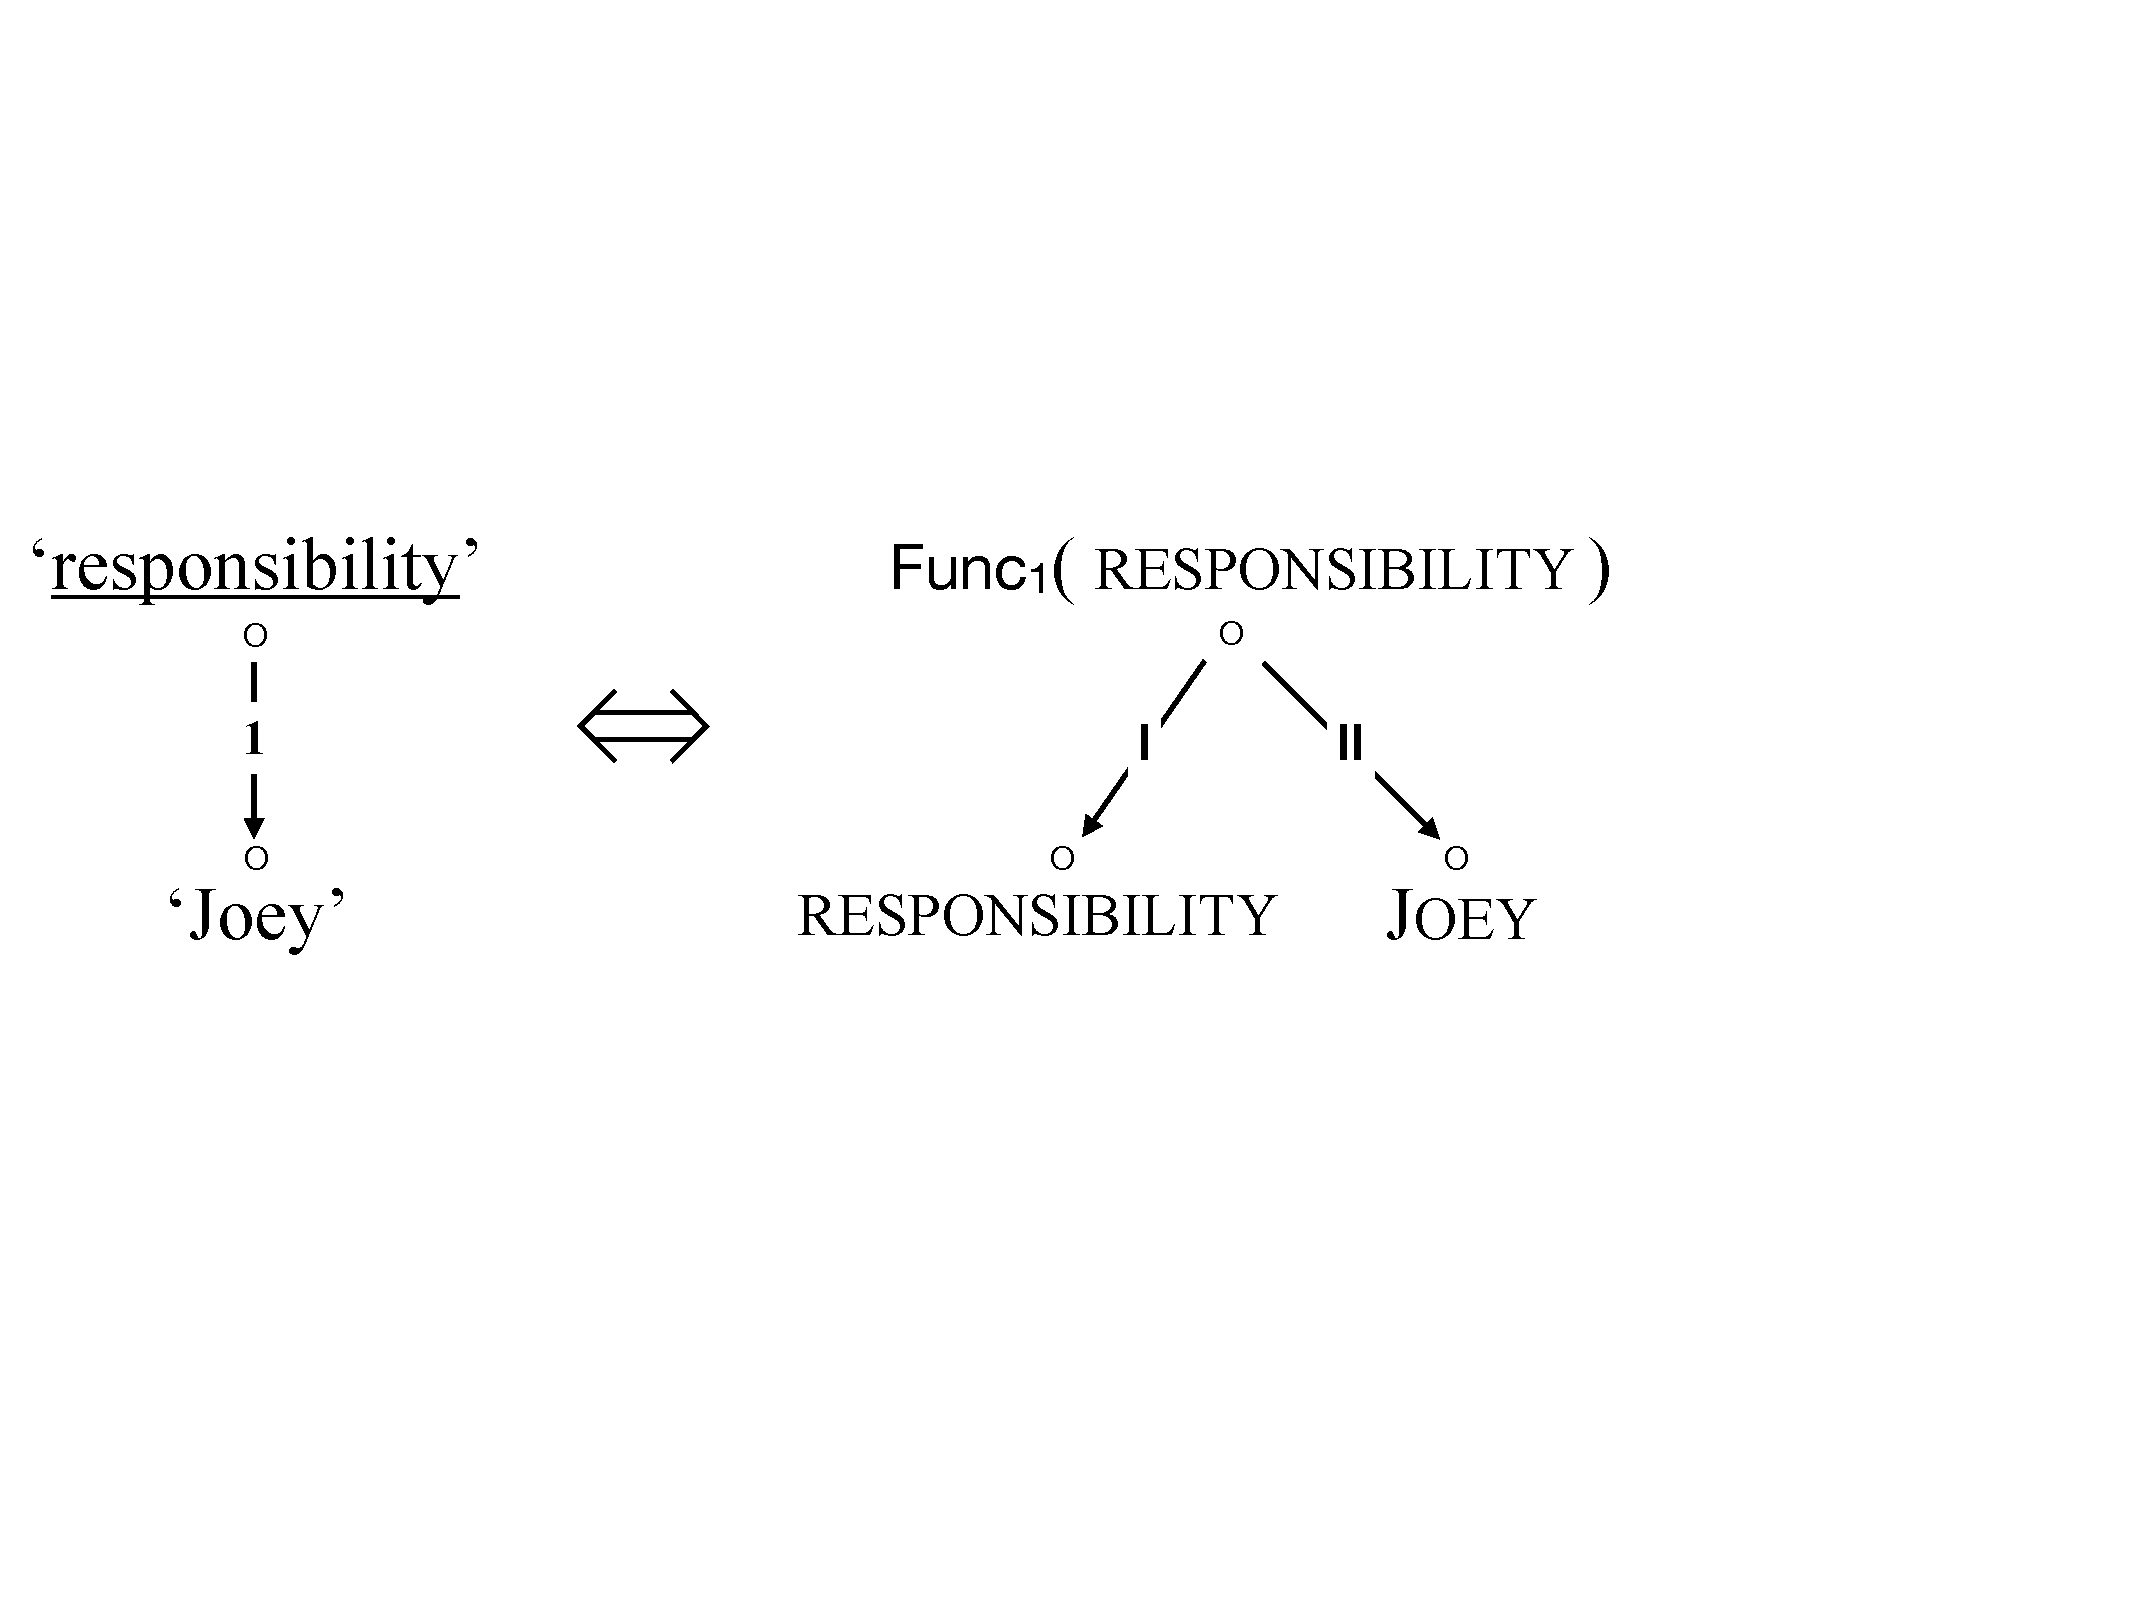
\includegraphics[height=22mm]{Fig/SyntLF/SemSyntFunc-i-illustr.pdf}
\caption{\lf{Func\tsub{1}} in the Sem\thinspace$\Leftrightarrow$\thinspace{}DSynt correspondence with L~=~\textsc{responsibility}}\label{fig:Func-i-illustr}
\end{figure}

Sentences \Next[a--b] are possible implementations of the DSynt-structure given in \figref{fig:Func-i-illustr}:

\begingroup
\small

\ex. \a. The responsibility \emph{lies} with Joey.
     \b. The responsibility \emph{rests} with Joey.

\endgroup

\begin{longtable*}[l]{ l l >{\raggedright\arraybackslash}p{6cm} }

\multicolumn{3}{l}{\textbf{English}} \\*

\lfappl{Func\tsub{0}}{\textit{thunder}\tsub{(N)}} & = & \textit{clap}\tsub{(V)}\textbf{,} \textit{crash}\tsub{(V)}\textbf{,} \textit{roll}\tsub{(V)}\textbf{,} \textit{rumble}\tsub{(V)} \\
\lfappl{Magn+Func\tsub{0}}{\textit{fire}\tsub{(N)} \lfgp{disaster}} & = & \textit{rage}\tsub{(V)} \\
\lfappl{Magn+Func\tsub{1}}{\textit{fire}\tsub{(N)} \lfgp{disaster}} & = & \textit{rip}\tsub{(V)}\textbf{,} \textit{sweep}\tsub{(V)} \lfgp{\textit{through} N\tsub{X}} \\
\lfappl{Func\tsub{1}}{\textit{responsibility} \lfgp{\textit{of} N\tsub{X}}} & = & \textit{lie}\tsub{(V)}\textbf{,} \textit{rest}\tsub{(V)} \lfgp{\textit{with} N\tsub{X}} \\
\lfappl{Func\tsub{1}}{\textit{smell}\tsub{(N)} \lfgp{\textit{of} N\tsub{X}}} & = & \textit{come}\tsub{(V)} \lfgp{\textit{from} N\tsub{X}} \\
\lfappl{Func\tsub{2}}{\textit{danger} \lfgp{\textit{for} N\tsub{Y}}} & = & \textit{threaten} \lfgp{N\tsub{Y}} \\
\lfappl{Func\tsub{2}}{\textit{accusation} \lfgp{\textit{against} N\tsub{Y}}} & = & \textit{hang}\tsub{(V)} \lfgp{\textit{over} N\tsub{Y}} \\
\lfappl{Func\tsub{3}}{\textit{conversation}} & = & \textit{be} \lfgp{\textit{about} N\tsub{Z}} \\*
\multicolumn{3}{l}{\quad\lfgp{\textit{conversation between {\upshape N\tsub{X}} and {\upshape N\tsub{Y}} about {\upshape N\tsub{Z}}}}} \\[6pt]

\multicolumn{3}{l}{\textbf{French}} \\*

\lfappl{Func\tsub{0}}{\textit{tonnerre}} & = & \textit{gronder}\textbf{,} \textit{retentir}\\
\lfappl{Magn+Func\tsub{0}}{\textit{incendie}} & = & \idiom{\textit{faire rage}}\\
\lfappl{Func\tsub{1}}{\textit{responsabilité} \lfgp{\textit{de} N\tsub{X}}} & = & \textit{incomber} \lfgp{\textit{à} N\tsub{X}}\\
\lfappl{Func\tsub{1}}{\textit{odeur} \lfgp{\textit{de} N\tsub{X}}} & = & \textit{se dégager}\textbf{,} \textit{émaner} \lfgp{\textit{de} N\tsub{X}}\\
\lfappl{Func\tsub{2}}{\textit{danger} \lfgp{\textit{pour} N\tsub{Y}}} & = & \textit{menacer} \lfgp{N\tsub{Y}}\\
\lfappl{Func\tsub{2}}{\textit{accusation} \lfgp{\textit{contre} N\tsub{Y}}} & = & \textit{frapper} \lfgp{N\tsub{Y}} \\
\lfappl{Func\tsub{3}}{\textit{conversation}} & = & \textit{porter} \lfgp{\textit{sur} N\tsub{Z}} \\*
\multicolumn{3}{l}{\quad\lfgp{\textit{conversation entre} N\tsub{X} \textit{et} N\tsub{Y} \textit{sur} N\tsub{Z}}} \\[6pt]

\multicolumn{3}{l}{\textbf{Russian}} \\*

\lfappl{Func\tsub{0}}{\textit{grom}} & = & \textit{gremet\palati}\textbf{,} \textit{gromyxat\palati} \\
\lfappl{Magn+Func\tsub{0}}{\textit{po\v{z}ar}} & = & \textit{bu\v{s}evat\palati} \\
\lfappl{Func\tsub{1}}{\textit{otvetstvennost\palati} \lfgp{N\tsub{X-\textsc{gen}}}} & = & \textit{le\v{z}at\palati} \lfgp{\textit{na}\sensenum{1} N\tsub{X-\textsc{prepos}}} \\
\lfappl{Func\tsub{1}}{\textit{zapax} \lfgp{N\tsub{X-\textsc{gen}}}} & = & \textit{idti}\textbf{,} \textit{isxodit\palati} \lfgp{\textit{ot} N\tsub{X-\textsc{gen}}} \\
\lfappl{Func\tsub{2}}{\textit{opasnost\palati} \lfgp{\textit{dlja} N\tsub{Y-\textsc{gen}}}} & = & \textit{grozit\palati}\textbf{,} \textit{ugro\v{z}at\palati} \lfgp{N\tsub{Y-\textsc{dat}}} \\
\lfappl{Func\tsub{2}}{\textit{obvinenie} \lfgp{\textit{protiv} N\tsub{Y-\textsc{gen}}}} & = & \textit{navisat\palati} \lfgp{\textit{nad} N\tsub{Y-\textsc{instr}}} \\
\lfappl{Func\tsub{3}}{\textit{razgovor}} & = & \textit{idti} \lfgp{\textit{o} N\tsub{Z-\textsc{prepos}}}\textbf{,} \textit{vertet\palati{}sja} \lfgp{\textit{vokrug} N\tsub{Z-\textsc{gen}}} \\
\multicolumn{3}{l}{\quad\lfgp{\textit{razgovor me\v{z}du} N\tsub{X-\textsc{instr}} \textit{i} N\tsub{Y-\textsc{instr}} \textit{o} N\tsub{Z-\textsc{prepos}}}} \\

\end{longtable*}

\refstepcounter{LFlist}
\subsubsection*{{\small [\arabic{LFlist}]} \lf{Labor\tsub{ij}} \lfgp{{\scriptsize Latin} \textit{labor\={a}re} `[to] work'}: support verb analogous to \textsc{submit} \lfgp{N\tsub{1}~\textit{to}~N\tsub{2}}}\label{lf:Labor-ij}
\addcontentsline{toc}{subsection}{{\footnotesize [\arabic{LFlist}]} \lf{Labor\tsub{ij}}: support verb analogous to \textsc{submit} \lfgp{N\tsub{1} \textit{to} N\tsub{2}}}\index[lf]{Laborij@\lf{Labor\tsub{ij}}|emph}

\lfappl{Labor\tsub{ij}}{L} is a support verb that takes L as its most oblique [=~most peripheral] DSyntA. Its DSyntA\thinspace\syntDname{I} corresponds to L's DSyntA\thinspace\syntDname{i} and its DSyntA\thinspace\syntDname{II} corresponds to L's DSyntA\thinspace\syntDname{j}.

\lf{Labor\tsub{ij}} participates in the Sem\thinspace$\Leftrightarrow$\thinspace{}DSynt\index[notion]{structure!semantic \tld\ [SemS]}\index[notion]{semantic!\tld\ structure [SemS]}\index[notion]{structure!deep-syntactic \tld\ [DSyntS]}\index[notion]{deep-syntactic!\tld\ structure [DSyntS]} correspondence\index[notion]{correspondence between representation levels} shown in \figref{fig:Labor-ij}; \figref{fig:Labor-ij-illustr} illustrates the correspondence template in \figref{fig:Labor-ij} for \lf{Labor\tsub{12}} with L~= \mbox{\textsc{applause}}.

\begin{figure}
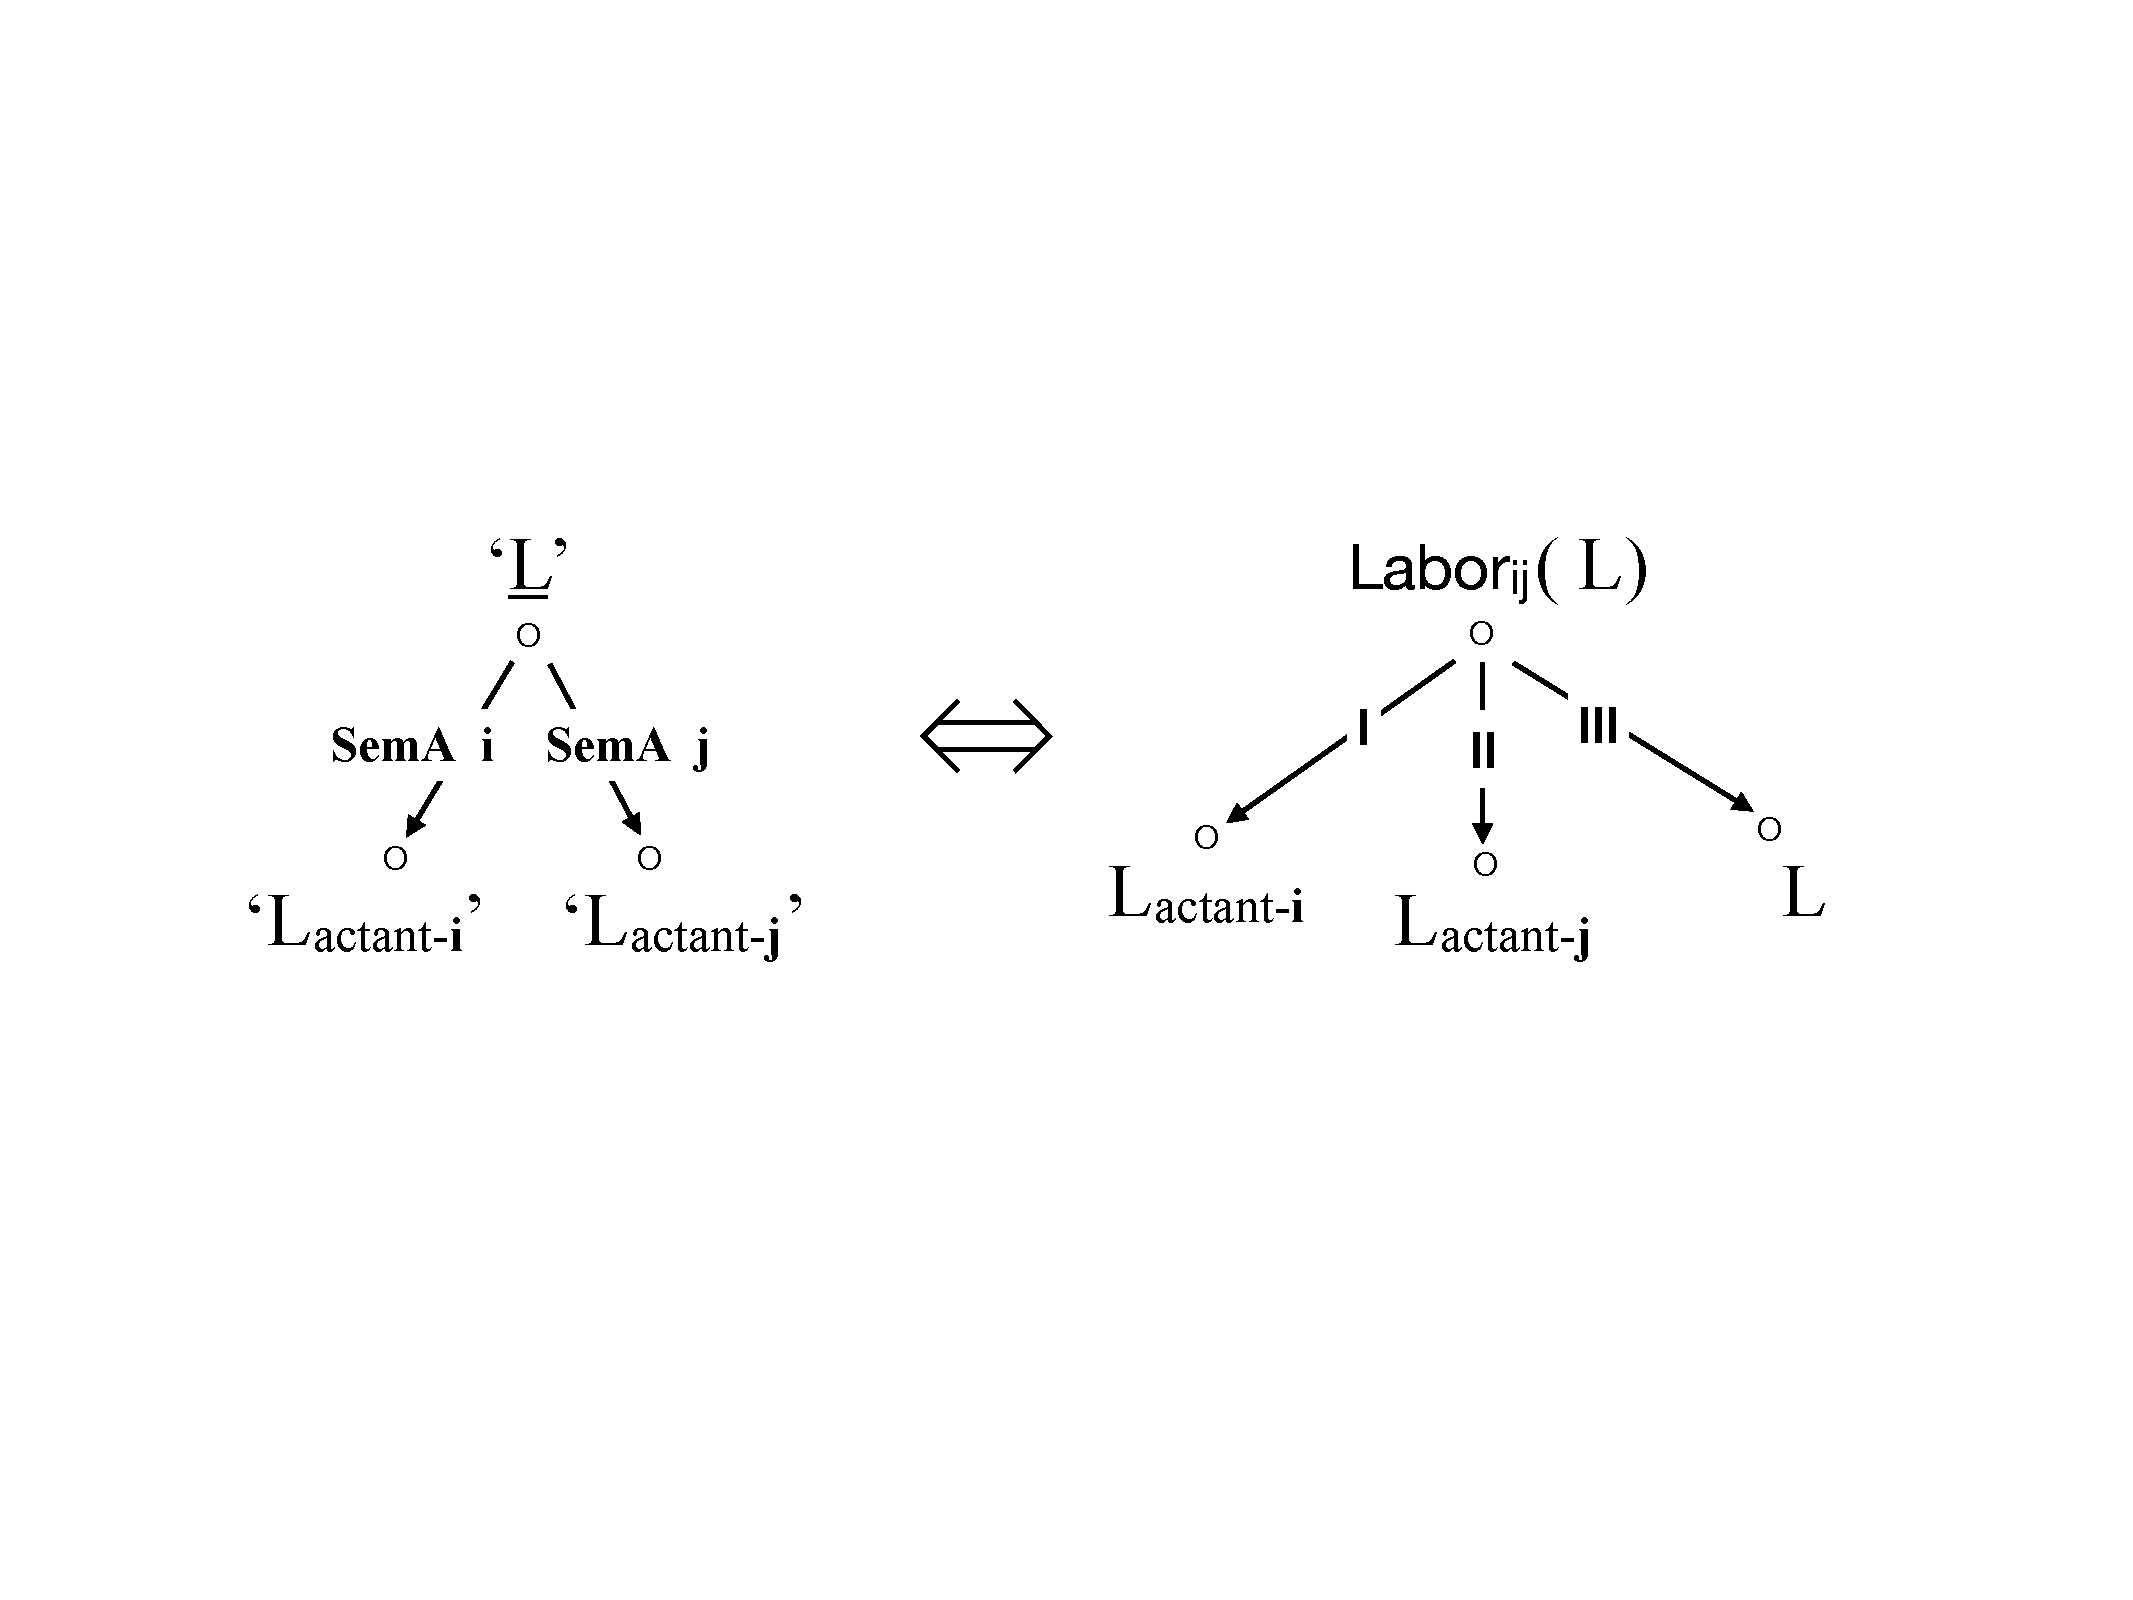
\includegraphics[width=0.65\linewidth]{Fig/SyntLF/SemSyntLabor-ij.pdf}
\caption{\lf{Labor\tsub{ij}} in the Sem\thinspace$\Leftrightarrow$\thinspace{}DSynt correspondence}\label{fig:Labor-ij}
\end{figure}

\begin{figure}
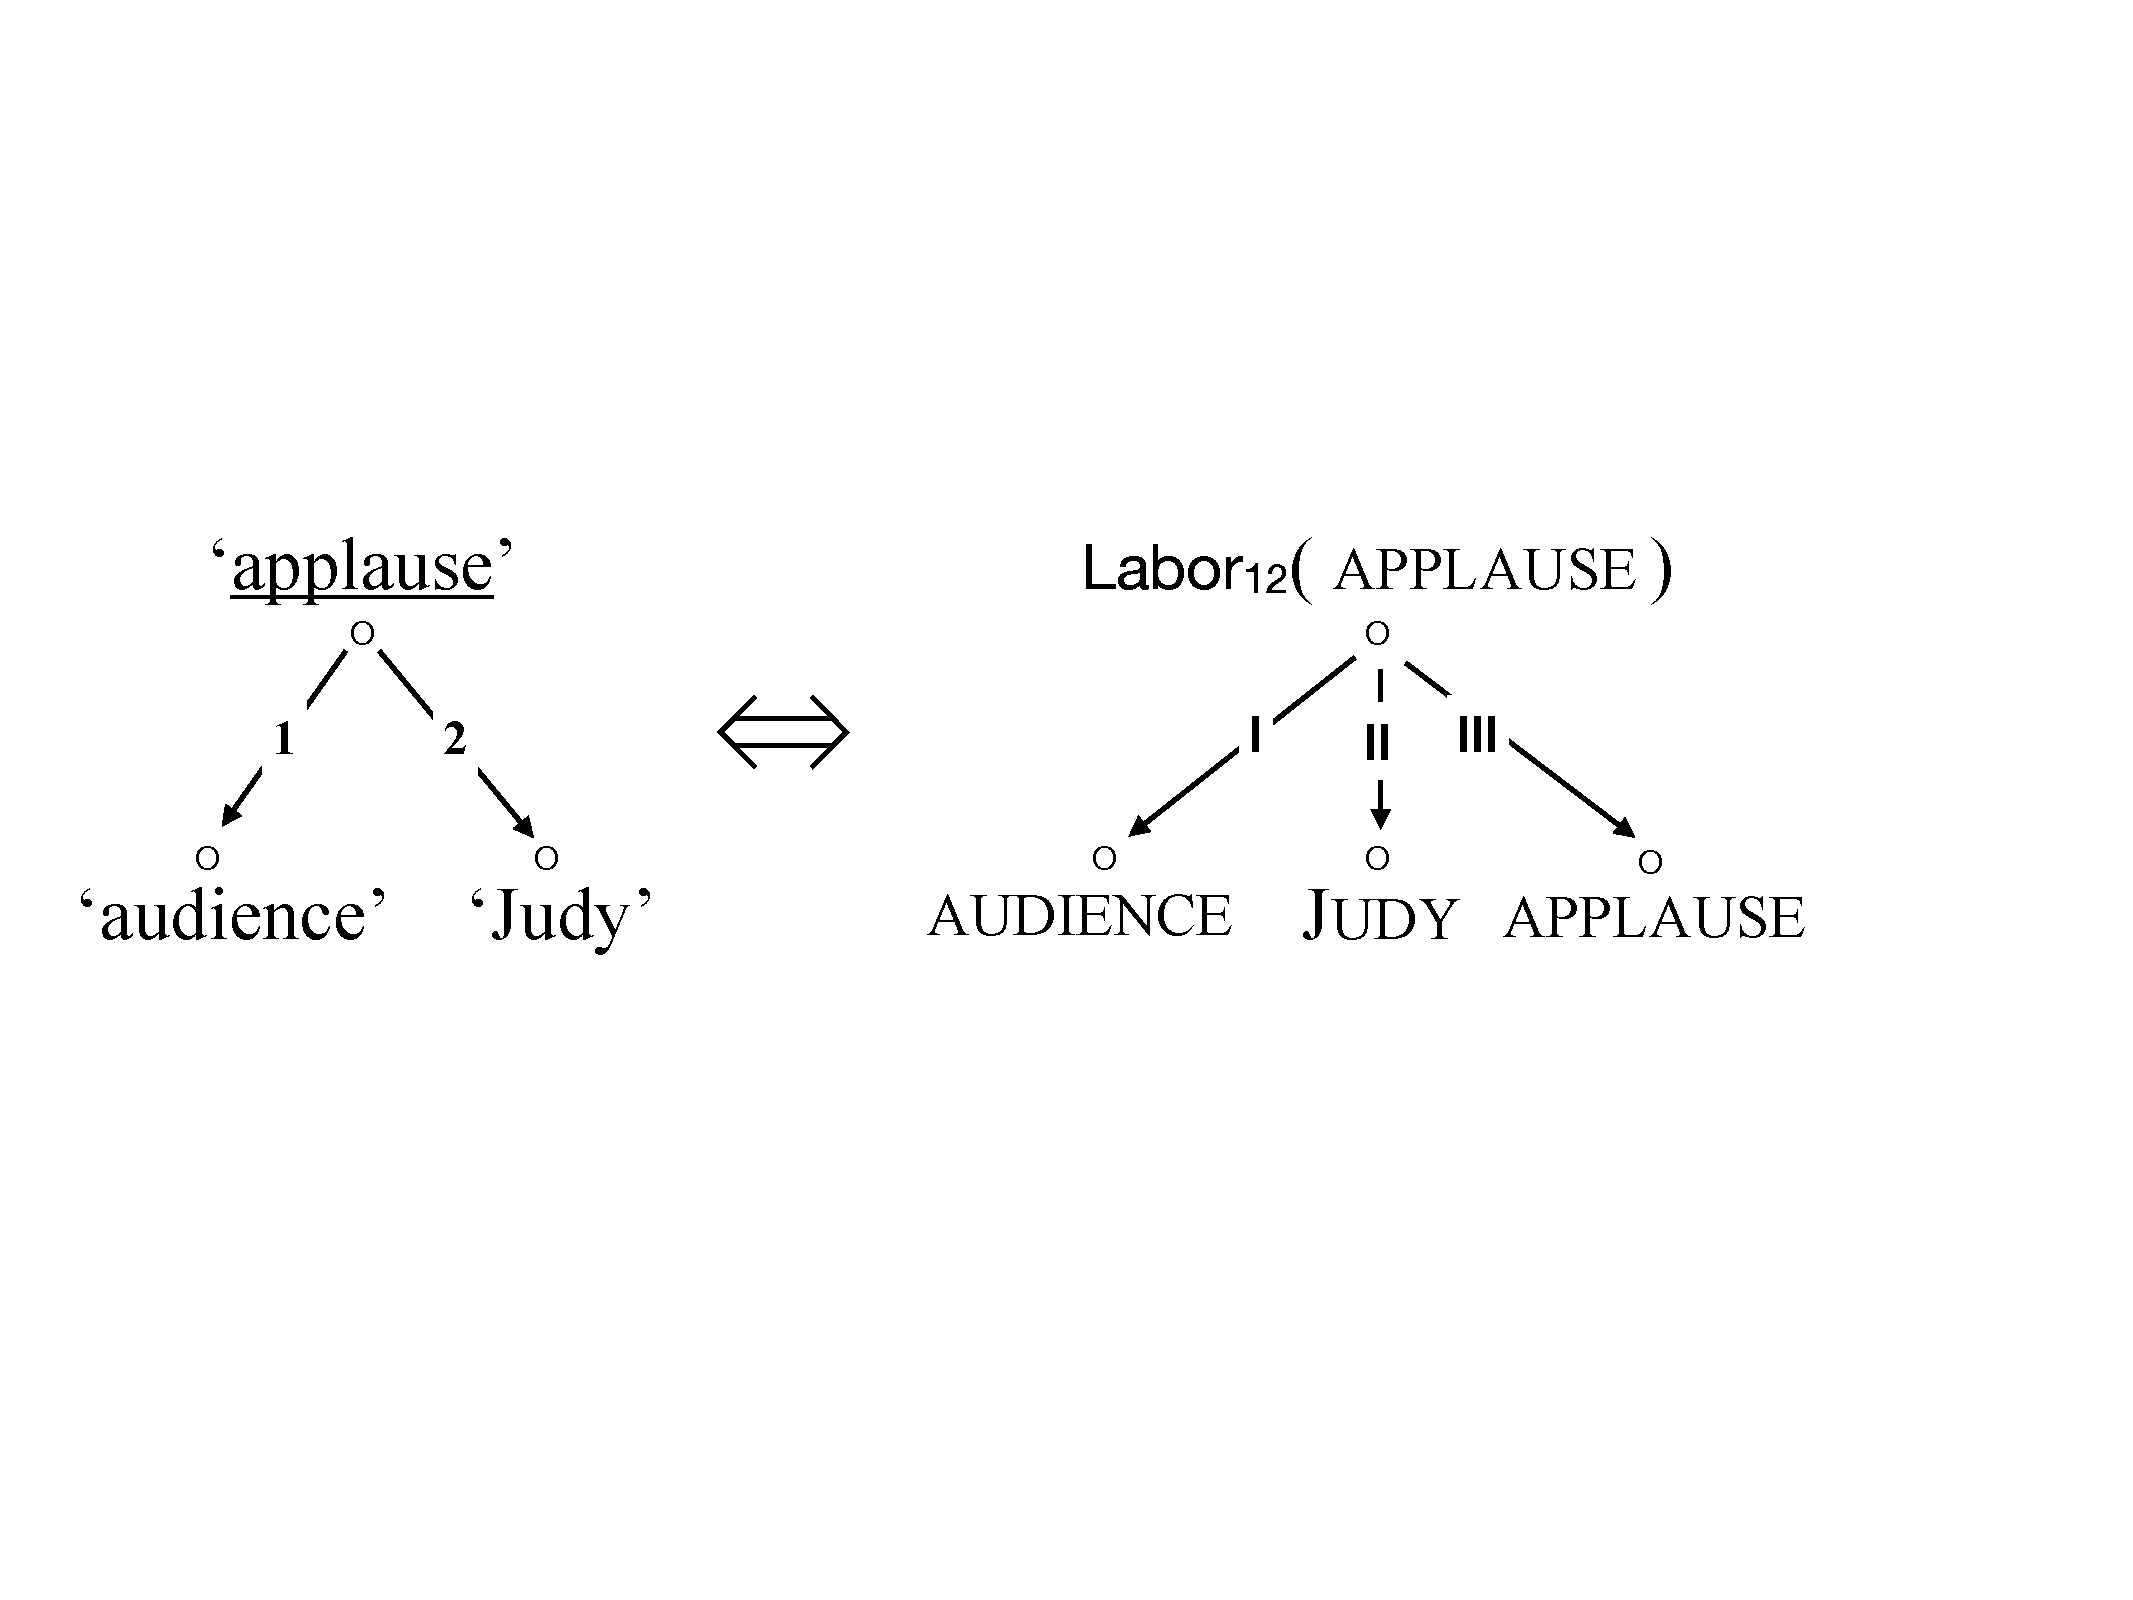
\includegraphics[width=0.65\linewidth]{Fig/SyntLF/SemSyntLabor-ij-illustr.pdf}
\caption{\lf{Labor\tsub{12}} in the Sem\thinspace$\Leftrightarrow$\thinspace{}DSynt correspondence with L~= \mbox{\textsc{applause}}}\label{fig:Labor-ij-illustr}
\end{figure}

The DSynt-structure given in \figref{fig:Labor-ij-illustr} is expressed by sentence \Next:

\begingroup
\small

\ex. The audience \emph{meets} Judy with applause.

\endgroup

\begin{longtable*}[l]{ l l >{\raggedright\arraybackslash}p{5cm} }

\multicolumn{3}{l}{\textbf{English}} \\*

\lfappl{Labor\tsub{12}}{\textit{esteem}\tsub{(N)} \lfgp{\textit{of} N\tsub{X} \textit{for} N\tsub{Y}}} & = & \textit{hold} \lfgp{N\tsub{Y} \textit{in} \tld} \\
\lfappl{Labor\tsub{12}}{\textit{use}\tsub{(N)} \lfgp{\textit{by} N\tsub{X} \textit{of} N\tsub{Y}}} & = & \textit{put} \lfgp{N\tsub{Y} \textit{to} \tld} \\
\lfappl{Labor\tsub{21}}{\lfgp{N\tsub{X},} \textit{result}\tsub{(N)} \lfgp{\textit{of} N\tsub{Y}}} & = & \textit{have} \lfgp{N\tsub{X} \textit{as a} \tld} \\[6pt]

\multicolumn{3}{l}{\textbf{French}} \\*

\lfappl{Labor\tsub{12}}{\textit{estime} \lfgp{\textit{de} N\tsub{X} \textit{pour}  N\tsub{Y}}} & = & \textit{avoir}\textbf{,} \textit{tenir} \lfgp{N\tsub{Y} \textit{en} \tld}\\
\lfappl{Labor\tsub{12}}{\textit{soins} \lfgp{\textit{de} N\tsub{X} \textit{destinés à}  N\tsub{Y}}} & = & \textit{entourer} \lfgp{N\tsub{Y} \textit{de} \tld}\\
\lfappl{Labor\tsub{21}}{\lfgp{N\tsub{X},} \textit{résultat} \lfgp{\textit{de} N\tsub{Y}}} & = & \textit{avoir} \lfgp{N\tsub{X} \textit{comme} \tld} \\[6pt]

\multicolumn{3}{l}{\textbf{Russian}} \\*

\lfappl{Labor\tsub{12}}{\textit{vlast\suffixsplit{}\palati} \lfgp{N\tsub{X-\textsc{gen}} \textit{nad} N\tsub{Y-\textsc{instr}}}} & = & \textit{der\v{z}at\palati} \lfgp{N\tsub{\textsc{acc}} \textit{pod} (\textit{svoej}) \tld\palat\textit{ju}} \\
\lfappl{Labor\tsub{12}}{\textit{zabot\suffixsplit{}a} \lfgp{N\tsub{X-\textsc{gen}} \textit{o} N\tsub{Y-\textsc{prepos}}}} & = & \textit{okru\v{z}it\palati} \lfgp{N\tsub{Y-\textsc{acc}} \tld\textit{oj}} \\*
\lfappl{Labor\tsub{21}}{\lfgp{N\tsub{X-\textsc{nom}},} \textit{rezul\palati{}tat} \lfgp{N\tsub{Y-\textsc{gen}}}} & = & \textit{imet\palati} \lfgp{N\tsub{X-\textsc{acc}} \tld\textit{om} $\langle$\textit{v ka\v{c}estve} \tld\textit{a}$\rangle$} \\

\end{longtable*}

\figref{fig:Labor-ij} and the above illustrations describe the prototypical case, where the argument L of \lf{Labor\tsub{ij}} is  bi-actantial. In such a case, \lfappl{Labor\tsub{ij}}{L} governs three \mbox{DSyntAs}, L filling the most oblique DSynt-slot. However, there are Ls with more than two DSyntAs. As a result of the transfer\index[notion]{actant!transfer of deep-syntactic \tld}\footnote{That is, syntactic raising -- see above, ``\nameref*{par:transferOfLsActants},'' p.\thinspace\pageref{par:transferOfLsActants}.}\index[notion]{raising, syntactic} of L's DSyntAs to the support verb, one obtains \lf{Labor} verbs with more than three DSyntAs. Take, for instance, the noun \textsc{inheritance} `belongings Y that X inherits from Z', and its French and Russian counterparts: they control three four-actantial \lf{Labor} collocates, as illustrated below.

\begin{longtable*}[l]{ l l >{\raggedright\arraybackslash}p{7cm} }

\multicolumn{3}{l}{\textbf{English}} \\*

\lfappl{Labor\tsub{123}}{\textit{inheritance}} & = & \textit{receive} \lfgp{N\tsub{Y$\Leftrightarrow${\tiny \textsf{\textbf{II}}}} \textit{from} N\tsub{Z$\Leftrightarrow${\tiny \textsf{\textbf{III}}}} \textit{as} \tld\tsub{L$\Leftrightarrow${\tiny \textsf{\textbf{IV}}}}} \\
\lfappl{Labor\tsub{321}}{\textit{inheritance}} & = & \textit{leave}\tsub{(V)} \lfgp{N\tsub{Y$\Leftrightarrow${\tiny \textsf{\textbf{II}}}} \textit{to} N\tsub{X$\Leftrightarrow${\tiny \textsf{\textbf{III}}}} \textit{as} \tld\tsub{L$\Leftrightarrow${\tiny \textsf{\textbf{IV}}}}} \\
\lfappl{Labor\tsub{213}}{\textit{inheritance}} & = & \textit{come}\tsub{(V)} \lfgp{\textit{to} N\tsub{X$\Leftrightarrow${\tiny \textsf{\textbf{II}}}} \textit{from} N\tsub{Z$\Leftrightarrow${\tiny \textsf{\textbf{III}}}} \textit{as} \tld\tsub{L$\Leftrightarrow${\tiny \textsf{\textbf{IV}}}}} \\[6pt]

\multicolumn{3}{l}{\textbf{French}} \\*

\lfappl{Labor\tsub{123}}{\textit{héritage}} & = & \textit{obtenir}\textbf{,} \textit{recevoir} \lfgp{N\tsub{Y$\Leftrightarrow${\tiny \textsf{\textbf{II}}}} \textit{de} N\tsub{Z$\Leftrightarrow${\tiny \textsf{\textbf{III}}}} \textit{en} \tld\tsub{L$\Leftrightarrow${\tiny \textsf{\textbf{IV}}}}}\\
\lfappl{Labor\tsub{321}}{\textit{héritage}} & = & \textit{laisser}\textbf{,} \textit{léguer} \lfgp{N\tsub{Y$\Leftrightarrow${\tiny \textsf{\textbf{II}}}} \textit{à} N\tsub{X$\Leftrightarrow${\tiny \textsf{\textbf{III}}}} \textit{en} \tld\tsub{L$\Leftrightarrow${\tiny \textsf{\textbf{IV}}}}} \\
\lfappl{Labor\tsub{213}}{\textit{héritage}} & = & \uslabel{specialized} \textit{échoir}\textbf{,} \textit{venir} \lfgp{\textit{à} N\tsub{X$\Leftrightarrow${\tiny \textsf{\textbf{II}}}} \textit{de} N\tsub{Z$\Leftrightarrow${\tiny \textsf{\textbf{III}}}} \textit{en} \tld\tsub{L$\Leftrightarrow${\tiny \textsf{\textbf{IV}}}}} \\[6pt]

\multicolumn{3}{l}{\textbf{Russian}} \\*

\lfappl{Labor\tsub{123}}{\textit{nasledstv\suffixsplit{}o}} & = & \textit{polu\v{c}it\palati} \lfgp{N\tsub{-\textsc{acc} Y$\Leftrightarrow${\tiny \textsf{\textbf{II}}}} \textit{ot} N\tsub{-\textsc{gen} Z$\Leftrightarrow${\tiny \textsf{\textbf{III}}}} \textit{v}\sensenum{2} \tld\textit{o}\tsub{L$\Leftrightarrow${\tiny \textsf{\textbf{IV}}}}}\\
\lfappl{Labor\tsub{321}}{\textit{nasledstv\suffixsplit{}o}} & = & \textit{ostavit\palati} \lfgp{N\tsub{-\textsc{acc} Y$\Leftrightarrow${\tiny \textsf{\textbf{II}}}} N\tsub{-\textsc{dat} X$\Leftrightarrow${\tiny \textsf{\textbf{III}}}} \textit{v}\sensenum{2} \tld\textit{o}\tsub{L$\Leftrightarrow${\tiny \textsf{\textbf{IV}}}}} \\
\lfappl{Labor\tsub{213}}{\textit{nasledstv\suffixsplit{}o}} & = & \textit{dostat\palati{}sja} \lfgp{N\tsub{-\textsc{dat} X$\Leftrightarrow${\tiny \textsf{\textbf{II}}}} \textit{ot} N\tsub{-\textsc{gen} Z$\Leftrightarrow${\tiny \textsf{\textbf{III}}}} \textit{v}\sensenum{2} \tld\textit{o}\tsub{L$\Leftrightarrow${\tiny \textsf{\textbf{IV}}}}} \\

\end{longtable*}

As we have seen, a collocational support verb \lf{Labor\tsub{ij}} relegates the collocation's base L  to the most oblique syntactic role: thus, L occupies the least privileged syntactic position, and this is anti-iconic\index[notion]{iconicity}. As a consequence, cases of \lf{Labor\tsub{ij}} are the least frequent ones among support verbs.

It is important to emphasize that the three support verb LFs are syntactically conversive\index[notion]{conversive} to each other, so that \lfappl{Func\tsub{1}}{L} $=$ \lfappl{Conv\tsub{21}Oper\tsub{1}}{L}, etc.:

\begingroup
\small

\ex. \a. \begingroup\setlength{\tabcolsep}{2pt}
\begin{tabular}[t]{ >{\raggedright\arraybackslash}p{2.6cm} c >{\raggedright\arraybackslash}p{7cm} }
\lfappl{Oper\tsub{1}}{\textit{analysis}} & = & \idiom{\textit{carry out}}\textbf{,} \textit{conduct}\tsub{(V)}\textbf{,} \textit{make}\tsub{(V)} \lfgp{\textsc{art} \tld} \\
\lfappl{Oper\tsub{2}}{\textit{analysis}} & = & \textit{undergo} \lfgp{\textsc{art} \tld} \\
\end{tabular}\endgroup
\b. \begingroup\setlength{\tabcolsep}{2pt}
\begin{tabular}[t]{ >{\raggedright\arraybackslash}p{2.6cm} c >{\raggedright\arraybackslash}p{7cm} }
\lfappl{Func\tsub{1}}{\textit{analysis}} & = & \textit{come}\tsub{(V)} \lfgp{\textit{from} N\tsub{X}} \\
\lfappl{Func\tsub{2}}{\textit{analysis}} & = & \textit{concern}\tsub{(V)} \lfgp{N\tsub{Y}} \\
\end{tabular}\endgroup
\c. \begingroup\setlength{\tabcolsep}{2pt}
\begin{tabular}[t]{ >{\raggedright\arraybackslash}p{2.6cm} c >{\raggedright\arraybackslash}p{7cm} }
\lfappl{Labor\tsub{12}}{\textit{analysis}} & = & \textit{subject}\tsub{(V)} \lfgp{N\tsub{Y} \textit{to} \textsc{art} \tld} \\
\end{tabular}\endgroup

\endgroup

To round off the present section, we will consider three cases of support verb\index[notion]{support verb!\tld\ with non-nominal base}\index[notion]{verb!support \tld\ with non-nominal base} collocations having a non-nominal base.

\begin{enumerate}

\item In SAE languages\index[notion]{Standard Average European [SAE] language}, all adjectives\index[notion]{adjective!\tld's support verb} used as attributive complement of a copula verb\index[notion]{copula verb}\index[notion]{verb!copula \tld} have the same ``joker''\index[notion]{value of an LF!joker \tld}\index[notion]{joker value of an LF}\index[notion]{lexical function!joker value of a \tld} \lf{Oper\tsub{1}}\index[lf]{Operi@\lf{Oper\tsub{i}}!joker \lf{Oper\tsub{1}}} support verb; for English, French and Russian: \textsc{be}\tsub{(copula)}\index[notion]{copula verb}\index[notion]{verb!copula \tld}, \textsc{être}\tsub{(copula)} and \textsc{byt\palat}\tsub{(copula)}.

\lfappl{Oper\tsub{1}}{L\tsub{(Adj)}} is equivalent to \lfappl{Copul}{L\tsub{(Adj)}}\index[lf]{Copul@\lf{Copul}} -- \sectref{sec:verbeCopule}, [\ref{lf:Copul}], p.\thinspace\pageref{lf:Copul}. Since the corresponding phrases are free (non-phraseologized), they are not to be considered here.

\item However, adjectives and adverbs denoting meteorological phenomena behave differently. They have a specific \lf{Oper\tsub{i}}: an impersonal \lf{Oper\tsub{0}}\index[notion]{verb!impersonal \tld}\index[notion]{impersonal verb}\index[lf]{Operi@\lf{Oper\tsub{i}}!\lf{Oper\tsub{0}}}.

\begin{longtable*}{ l l >{\raggedright\arraybackslash}p{6.5cm} }

\multicolumn{3}{l}{\textbf{English}} \\*

\lfappl{Oper\tsub{0}}{\textit{hot}\slashs\textit{misty}} & = & \lfgp{\textit{it}\tsub{(impers)}} \textit{be}\tsub{(meteo)} \lfgp{\tld} \\*
& & {\small\textit{It was hot}\thinspace/\thinspace\textit{misty in Montreal.}} \\[3pt]

\multicolumn{3}{l}{\textbf{French}} \\*

\lfappl{Oper\tsub{0}}{\textit{chaud}} & = & \lfgp{\textit{il}\tsub{(impers)}} \textit{faire}\tsub{(meteo)} \lfgp{\tld}\\
& & {\small\textit{Il faisait chaud à Montréal.}} \\
\lfappl{Oper\tsub{0}}{\textit{brumeux}} & = & \lfgp{\textit{il}\tsub{(impers)}} \textit{faire}\tsub{(meteo)}\textbf{,} \lfgp{\textit{ce}\tsub{(impers)}} \textit{être}\tsub{(meteo)} \lfgp{\tld} \\*
& & {\small\textit{Il faisait} $\langle$\textit{C'était}$\rangle$ \textit{brumeux à Montréal.}} \\[3pt]

\multicolumn{3}{l}{\textbf{Russian}} \\*

\lfappl{Oper\tsub{0}}{\textit{\v{z}arko}\slashs\textit{tumanno}} & = & \lfgp{Ø\tsub{(impers)}} \textit{byt\palati}\tsub{(meteo)} \lfgp{\tld} \\
& & {\small\textit{V Monreale bylo \v{z}arko{\upshape \slashs}tumanno.}} \vspace{6pt} \\

\end{longtable*}

\item \idiom{Prep\thinspace$\rightarrow$\thinspace{}N} adverbial idioms having several \lf{Oper\tsub{1}} collocates are not uncommon, as illustrated by the English idiom \idiom{\textsc{on cloud nine}} `extremely happy':\footnote{See also \textcite[136]{MelcukPolguere2021} for a detailed analysis of the French idiom  \idiom{\textsc{dans la semoule}} (lit.~`in the semolina') `not knowing what to do in a difficult situation' and its \lf{Oper\tsub{1}} collocates: \textit{être} `be', \textit{nager} `swim', \textit{patauger} `wade' and \textit{pédaler} `pedal'.}

\begingroup
\small

\ex. \begingroup\setlength{\tabcolsep}{2pt}
\begin{tabular}[t]{ l l >{\raggedright\arraybackslash}p{7cm} }
\lfappl{Oper\tsub{1}}{\idiom{\textit{on cloud nine}}} & = & \textit{be}\textbf{,} \textit{float}\tsub{(V)}\textbf{,} \textit{fly}\tsub{(V)} \lfgp{\tld} \\
\end{tabular}\endgroup

\endgroup

\end{enumerate}

\subsection{Realization verbs}\label{sec:verbeReal}

\index[notion]{realization verb|emph}\index[notion]{verb!realization \tld|emph}This section introduces three types of verbal collocates that are similar in their syntactic behavior to the three support verbs described in the previous section. Semantically, however, \notion{realization verbs} are very different. They are not empty, but express a specific meaning: `fulfill an inherent requirement of L' -- in the most general sense (more specifically, `realize', `use', `accomplish', etc.). This semantic load justifies the name \emph{realization verbs}. Just as the support verb LFs, the three realization verb LFs are mutual conversives\index[notion]{conversive}.

A fourth LF that is semantically related to realization verb LFs is also introduced at the end of this section: \lf{Prepar}. It is, so to speak, a realization verb by extension.

All four verbal LFs presented in this section have the same PoS table:

\begin{quote}
\begingroup
\phantomsection\label{tab:PdDVReal}\small
\begin{tabular}{ l c c }
   \midrule
   \multicolumn{3}{l}{\lf{Real\tsub{i}}, \lf{Fact\tsub{i}}, \lf{Labreal\tsub{ij}}, \lf{Prepar}: verbal} \\
   \midrule
   \textbf{L} & \cellcolor[gray]{0.85}V & N \\
   \midrule
\textbf{\lfappl{Real\tsub{i}\slashs{}Fact\tsub{i}\slashs{}Labreal\tsub{ij}\slashs{}Prepar}{L}} & \cellcolor[gray]{0.85}V & V \\
   \midrule
\end{tabular}
\endgroup
\end{quote}

This table shows that the realization verbs prototypically have a nominal base. The shading of the column for verbal bases indicates that these cases present some complications -- see ``\nameref*{par:RealVFusion}'' below, p.\thinspace\pageref{par:RealVFusion}.

\refstepcounter{LFlist}
\subsubsection*{{\small [\arabic{LFlist}]} \lf{Real\tsub{i}} \lfgp{{\scriptsize Latin} \textit{realis} `real'}
: realization verb that means `fulfill [L]'} \label{lf:Real-i}
\addcontentsline{toc}{subsection}{{\footnotesize [\arabic{LFlist}]} \lf{Real\tsub{i}}: realization verb that means `fulfill \lfgp{L}'}\index[lf]{Reali@\lf{Real\tsub{i}}|emph}

\lfappl{Real\tsub{i}}{L} is a realization verb that takes L as DSyntA\thinspace\syntDname{II} and the DSyntA\thinspace\syntDname{i} of L as DSyntA\thinspace\syntDname{I}. It controls the same syntactic structure as support verbs of the type \lf{Oper\tsub{i}}\index[lf]{Operi@\lf{Oper\tsub{i}}}.

\begin{longtable*}[l]{ l l >{\raggedright\arraybackslash}p{6cm} }

\multicolumn{3}{l}{\textbf{English}} \\*

\lfappl{Real\tsub{1}}{\textit{promise}\tsub{(N)}} & = & \textit{keep} \lfgp{\textsc{art} \tld} \\
\lfappl{Real\tsub{2}}{\textit{expectations}} & = & \idiom{\textit{come up}} \lfgp{\textit{to} \textsc{art} \tld}\textbf{,} \textit{fulfill} \lfgp{\textsc{art} \tld}\textbf{;} \idiom{\textit{live up}} \lfgp{\textit{to} \textsc{art} \tld} \\
\lfappl{Real\tsub{3}}{\textit{order}\tsub{(N)}} & = & \idiom{\textit{carry out}}\textbf{,} \textit{execute}\textbf{,} \textit{fulfill} \lfgp{\textsc{art} \tld} \\
\multicolumn{3}{l}{\quad\lfgp{N\tsub{X}\textit{'s order to} V\tsub{Y} \textit{to} N\tsub{Z}}} \\
\lfappl{Real\tsub{1}}{\textit{plane}\tsub{(N)}} & = & \textit{pilot}\tsub{(V)} \lfgp{\textsc{art} \tld} \\[6pt]

\multicolumn{3}{l}{\textbf{French}} \\*

\lfappl{Real\tsub{1}}{\textit{promesse}} & = & \textit{tenir} \lfgp{\textsc{art} \tld}\\
\lfappl{Real\tsub{2}}{\textit{attentes}} & = & \textit{répondre} \lfgp{\textit{à} \textsc{art} \tld}\\
\lfappl{Real\tsub{3}}{\textit{ordre}} & = & \textit{exécuter}\textbf{,} \textit{suivre} \lfgp{\textsc{art} \tld}\\
\multicolumn{3}{l}{\quad\lfgp{\textit{ordre de} N\tsub{X} \textit{de} V\tsub{Y-\textsc{inf}} \textit{à} N\tsub{Z}}} \\
\lfappl{Real\tsub{1}}{\textit{avion}} & = & \textit{piloter} \lfgp{\textsc{art} \tld}\\
\lfappl{Real\tsub{1}}{\idiom{\textit{chasse d'eau}}} & = & \textit{actionner}\textbf{,} \textit{activer}\textbf{,} \textit{tirer} \lfgp{\textsc{art} \tld} \\[6pt]

\multicolumn{3}{l}{\textbf{Russian}} \\*

\lfappl{Real\tsub{1}}{\textit{obe\v{s}\v{c}ani\suffixsplit{}e}} & = & \textit{sder\v{z}at\palati}\textbf{,} \textit{vypolnit\palati} \lfgp{ \tld\textit{e}} \\
\lfappl{Real\tsub{2}}{\textit{ožidani\suffixsplit{}ja}} & = & \textit{opravdat\palati} \lfgp{\tld\textit{ja}} \\
\lfappl{Real\tsub{3}}{\textit{prikaz}} & = & \textit{vypolnit\palati} \lfgp{\tld} \\*
\multicolumn{3}{l}{\quad\lfgp{\textit{prikaz} N\tsub{X-\textsc{gen}} V\tsub{Y-\textsc{inf}} N\tsub{Z-\textsc{dat}}}} \\*
\lfappl{Real\tsub{1}}{\textit{samolët}} & = & \textit{pilotirovat\palati}\textbf{,} \textit{vesti} \lfgp{\tld} \\

\end{longtable*}

The argument L of \lf{Real\tsub{i}} -- just as of the two other realization verbs -- must contain in its lexicographic definition\index[notion]{definition!lexicographic \tld} at least one particular semantic component which expresses a ``requirement'' of L and thus is compatible with the meaning of realization. It is this component that is the target\index[notion]{target of an LF}\index[notion]{lexical function!target of a \tld} for \lf{Real\tsub{i}}.\footnote{See the presentation of targets of LFs in \chapref{chap:NotionLF}, \sectref{sec:classeFLSyntagmatiques}, p.\thinspace\pageref{txt:targetOfSyntLF}.} Consider, for instance, the definition of the noun \textsc{debt}:

\begingroup
\small

\ex. \label{ldef:defDEBT}\APolbox{9.3cm}{%
   \begin{tabular}{ l p{5.6cm} }
   \textit{X's debt of Y to Z} :
   &
   sum of money Y that X got from Z \newline
   \setlength{\tabcolsep}{.5pt}\begin{tabular}{ p{0.2cm} >{\raggedright\arraybackslash}p{5.3cm} }
   \SpecDiff &  that X \emph{is expected to \idiom{pay back}} to Z \\
   \end{tabular} \\
\end{tabular}
}

\endgroup

The emphasized component (`is expected to \idiom{pay back}') corresponds to the inherent requirement of \textsc{debt}, which is targeted
in the \lf{Real\tsub{1}} collocations: \textit{clear}, \idiom{\textit{pay back}}, \idiom{\textit{pay off}}, \textit{repay a debt}.

\paragraph*{Degree of realization.}\label{par:degreesOfReal}

The elements of the value of \lfappl{Real\tsub{i}}{L} may differ by the degree of realization\index[notion]{degree of realization}. Three degrees are distinguished, using the superscripts \lf{\tsup{I}}, \lf{\tsup{II}} and \lf{\tsup{III}}\index[lf]{Reali@\lf{Real\tsub{i}}!\lf{Real\tsub{1}}@\lf{Real$_\text{1}^\text{I}$}|emph}:

\begingroup
\small

\ex. \a. \begingroup\setlength{\tabcolsep}{2pt}
\begin{tabular}[t]{ l l >{\raggedright\arraybackslash}p{7cm} }
\lfappl{Real$_\text{1}^\text{I}$}{\textit{suitcase}} & = & \textit{fill}\tsub{(V)}\textbf{,} \textit{pack}\tsub{(V)} \lfgp{\textsc{art} \tld} \\
\lfappl{Real$_\text{1}^\text{II}$}{\textit{suitcase}} & = & \textit{carry}\tsub{(V)} \lfgp{\textsc{art} \tld}\textbf{;} \textit{drag}\tsub{(V)} \lfgp{\textsc{art} \tld}\textbf{;} \textit{wheel}\tsub{(V)} \lfgp{\textsc{art} \tld} \\
\lfappl{Real$_\text{1}^\text{III}$}{\textit{suitcase}} & = & \textit{empty}\tsub{(V)}\textbf{,} \textit{unpack} \lfgp{\textsc{art} \tld} \\
\end{tabular}\endgroup
\b. \begingroup\setlength{\tabcolsep}{2pt}
\begin{tabular}[t]{ l l >{\raggedright\arraybackslash}p{7cm} }
\lfappl{Real$_\text{2}^\text{I}$}{\textit{task}\tsub{(N)}} & = & \textit{tackle}\tsub{(V)} \lfgp{\textsc{art} \tld} \\
\lfappl{Real$_\text{2}^\text{II}$}{\textit{task}\tsub{(N)}} & = & \textit{fulfill} \lfgp{\textsc{art} \tld} \\
\end{tabular}\endgroup
%\lfappl{Real\textsubscript{\raisebox{-1pt}{\rlap{2}}}\textsuperscript{\raisebox{1pt}{I}}}{\textit{peine} \lfgp{jurid.}} & = & \textit{recevoir} \lfgp{\textsc{art} \tld}\\
%\lfappl{Real\textsubscript{\raisebox{-1pt}{\rlap{2}}}\textsuperscript{\raisebox{1pt}{II}}}{\textit{peine} \lfgp{jurid.}} & = & \textit{purger} \lfgp{\textsc{art} \tld}\\
%\lfappl{Real\textsubscript{\raisebox{-1pt}{\rlap{2}}}\textsuperscript{\raisebox{1pt}{I}}}{\textit{livre}} & = & \textit{ouvrir} \lfgp{\textsc{art} \tld}\\
%\lfappl{Real\textsubscript{\raisebox{-1pt}{\rlap{2}}}\textsuperscript{\raisebox{1pt}{II}}}{\textit{livre}} & = & \textit{lire} \lfgp{\textsc{art} \tld}\\

\endgroup

Some details on the distinction between \lf{Real$_\text{i}^\text{I}$} and the LF \lf{Prepar}\index[lf]{Prepar@\lf{Prepar}} are given below ([\ref{lf:Prepar}], p.\thinspace\pageref{it:diffPreparReal1--I}).

\paragraph*{External participant as realizer.}\label{par:RealOmega}

The ``realizer'' of \lfappl{Real\tsub{i}}{L} can be an external participant\index[notion]{participant of a situation!external \tld} of the situation denoted by L  (cf. \chapref{chap:preliminaryNotions}, \sectref{sec:semanticNotions}, p.\thinspace\pageref{par:externalParticipant}). In such cases, a special actantial subscript\index[notion]{actantial subscript!\tld\ \textOmega} \textOmega\ is used: \lf{Real\tsub{\textOmega}}\index[lf]{Reali@\lf{Real\tsub{i}}!\lf{Real\tsub{\textOmega}}|emph}. The symbol \textOmega\ indicates that the DSyntA\thinspace\syntDname{I} of \lfappl{Real\tsub{\textOmega}}{L} does not correspond to one of L's DSyntAs. Here are a few illustrations:

\begingroup
\small

\ex. \begingroup\setlength{\tabcolsep}{2pt}
\begin{tabular}[t]{ l l >{\raggedright\arraybackslash}p{7cm} }
\lfappl{Real\tsub{\textOmega}}{\textit{mountain}} & = &  \textit{climb}\tsub{(V)}\textbf{,} \textit{scale}\tsub{(V)} \lfgp{\textsc{art} \tld} \\
\lfappl{Real\tsub{\textOmega}}{\textit{costs}\tsub{(N)}} & = &  \textit{cover}\tsub{(V)} \lfgp{\textsc{art} \tld} \\
\lfappl{Real\tsub{\textOmega}}{\textit{baby}\tsub{(N)}} & = & \idiom{\textit{take care}} \lfgp{\textit{of} \textsc{art} \tld}\textbf{,} \fused\textit{babysit} \\
\lfappl{Real\tsub{\textOmega}}{\textit{pulse}\tsub{(N)}} & = & \textit{feel}\tsub{(V)}\textbf{,} \textit{take}\tsub{(V)} \lfgp{\textsc{art} \tld} \\
%\lfappl{Real\tsub{\textOmega}}{\textit{épidémie}} & = & \textit{combattre} \lfgp{\textsc{art} \tld}\textbf{,} \textit{lutter} \lfgp{\textit{contre} \textsc{art} \tld}\\
%\lfappl{Real\tsub{\textOmega}}{\textit{dette}} & = & \idiom{\textit{prendre en charge}} \lfgp{\textsc{art} \tld}\\
%\lfappl{Real\tsub{\textOmega}}{\textit{bébé}} & = & \textit{s'occuper} \lfgp{\textit{de} \textsc{art} \tld}\textbf{;} \textit{garder} \lfgp{\textsc{art} \tld}\\
%\lfappl{Real\tsub{\textOmega}}{\textit{pouls}} & = & \textit{prendre} \lfgp{\textsc{art} \tld\ \textit{à} N\tsub{X}}\textbf{,} \textit{tâter} \lfgp{\textsc{art} \tld}\\
\end{tabular}\endgroup

\endgroup

\begin{historicalremark}
In previous lexicographic projects -- in particular, in the development of the \notion{DiCo} lexical database \parencite{Polguere2000b} --, subscripts $\lozenge$ or @ have been used in place of \textOmega.
\end{historicalremark}\index[notion]{lexical database!DiCo}\index[notion]{DiCo}

\paragraph*{Verbal argument of \lf{Real\tsub{i}}.}\label{par:RealVFusion}

\lf{Real\tsub{i}} can also apply to a verb. In this case, \lfappl{Real\tsub{i}}{L} normally gives fused\index[notion]{fusion}\index[notion]{value of an LF!fused \tld} values:

\begingroup
\small

\ex. \begingroup\setlength{\tabcolsep}{2pt}
\begin{tabular}[t]{ l l >{\raggedright\arraybackslash}p{7cm} }
\lfappl{Real\tsub{1}}{\textit{approach}\tsub{(V)} \lfgp{N\tsub{Y}}} & = & \fused\textit{reach}\tsub{(V)} \lfgp{N\tsub{Y}} \\
\lfappl{Real\tsub{1}}{\textit{look}\tsub{(V)} \lfgp{for N\tsub{Y}}} & = & \fused\textit{find}\tsub{(V)} \lfgp{N\tsub{Y}} \\
\lfappl{Real\tsub{1}}{\textit{pursue} \lfgp{N\tsub{Y}}} & = & \fused\textit{catch}\tsub{(V)} \lfgp{N\tsub{Y}} \\
\lfappl{Real\tsub{1}}{\textit{stagger}\tsub{(V)}} & = & \fused\textit{fall}\tsub{(V)} \\
\lfappl{Real\tsub{2}}{\textit{rock}\tsub{(V)} \lfgp{N\tsub{Y}}} & = & \fused\textit{fall asleep} \\
%\lfappl{Real\tsub{1}}{\textit{s'approcher} \lfgp{\textit{de} N\tsub{Y}}} & = & \fused\textit{atteindre} \lfgp{N\tsub{Y}}\footnotemark \\
%\lfappl{Real\tsub{1}}{\textit{chercher}} & = & \fused\textit{trouver} \\
%\lfappl{Real\tsub{1}}{\textit{poursuivre}} & = & \fused\textit{attraper} \\
%\lfappl{Real\tsub{1}}{\textit{basculer}} & = & \fused\textit{tomber} \\
%\lfappl{Real\tsub{2}}{\textit{bercer}} & = & \fused\textit{s'endormir} \\
%Real1(približat´sja  [k NY]) =  dostič´ [NY-a]
%Real1(iskat´) = najti
%Real1(lovit´) = pojmat´
%Real1(pošatnut´sja) = upast´
%Real2(ukačivat´) = zasnut´
%\footnotetext{Comparer avec \lfappl{Result\tsub{1}}{\textit{atteindre} \lfgp{\textit{de} N\tsub{Y}}} = \textit{être} \lfgp{\lf{Loc\tsub{in}} N\tsub{Y}} -- \chapref{chap:paraLFs}, [\ref{lf:Result-i}], p.\thinspace\pageref{lf:Result-i}.}
\end{tabular}\endgroup

\endgroup

These fused \lfappl{Real\tsub{i}}{L} should not be mistaken for cases of \lfappl{Result\tsub{i}}{L}\index[lf]{Resulti@\lf{Result\tsub{i}}}, which are in a \emph{paradigmatic}\index[notion]{lexical function!paradigmatic vs. syntagmatic \tlds} relation with L (\chapref{chap:paraLFs}, [\ref{lf:Result-i}], p.\thinspace\pageref{lf:Result-i}). The situation denoted by \lfappl{Real\tsub{i}}{L}, contrary to \lfappl{Result\tsub{i}}{L}, is not necessarily a result of the situation denoted by L. For instance, one can fall asleep without being rocked -- cf. last illustration in \Last.

\paragraph*{Frequent combination with \lf{Anti}.}

Because it is not semantically empty, \lf{Real\tsub{i}} -- and the two other LFs of realization as well -- frequently combines with \lf{Anti}\index[lf]{Anti@\lf{Anti}}. As a result, \lfappl{AntiReal\tsub{i}}{L}\phantomsection\label{lf:AntiReal-i}\index[lf]{Reali@\lf{Real\tsub{i}}!\lf{AntiReal\tsub{i}}|emph} expresses the meaning `do the opposite of fulfilling an inherent requirement of~L'.

\begingroup
\small

\ex. \a. \begingroup\setlength{\tabcolsep}{2pt}
\begin{tabular}[t]{ >{\raggedright\arraybackslash}p{3.4cm} l >{\raggedright\arraybackslash}p{5cm} }
\lfappl{Real\tsub{1}}{\textit{impulse}\tsub{(N)}} & = & \textit{yield}\tsub{(V)} \lfgp{\textit{to} \textsc{art} \tld} \\*
\lfappl{AntiReal\tsub{1}}{\textit{impulse}\tsub{(N)}} & = & \textit{control}\tsub{(V)}\textbf{,} \textit{resist}\tsub{(V)} \lfgp{\textsc{art} \tld} \\
\end{tabular}\endgroup
\b. \begingroup\setlength{\tabcolsep}{2pt}
\begin{tabular}[t]{ >{\raggedright\arraybackslash}p{3.4cm} l >{\raggedright\arraybackslash}p{5cm} }
\lfappl{Real\tsub{1}}{\idiom{\textit{red light}}} & = & \textit{stop}\tsub{(V)} \lfgp{\textit{at} \textsc{art} \tld} \\*
\lfappl{AntiReal\tsub{1}}{\idiom{\textit{red light}}} & = & \textit{jump}\tsub{(V)}\textbf{,} \textit{run}\tsub{(V)} \lfgp{\textsc{art} \tld} \\
\end{tabular}\endgroup
\c. \begingroup\setlength{\tabcolsep}{2pt}
\begin{tabular}[t]{ >{\raggedright\arraybackslash}p{3.4cm} l >{\raggedright\arraybackslash}p{5cm} }
\lfappl{Real\tsub{2}}{\textit{exam}} & = & \textit{pass}\tsub{(V)} \lfgp{\textsc{art} \tld} \\*
\lfappl{AntiReal\tsub{2}}{\textit{exam}} & = & \textit{fail}\tsub{(V)} \lfgp{\textsc{art} \tld} \\
%\lfappl{Real\tsub{1}}{\textit{pulsion}} & = & \textit{céder} \lfgp{à \textsc{art} \tld} \\
%\lfappl{AntiReal\tsub{1}}{\textit{pulsion}} & = & \textit{contrôler} \lfgp{\textsc{art} \tld} \\
%\\
%\lfappl{Real\tsub{1}}{\idiom{\textit{feu rouge}}} & = & \textit{s'arrêter} \lfgp{à \textsc{art} \tld}\textbf{;} \\
 %& & \textit{respecter} \lfgp{\textsc{art} \tld} \\
%\lfappl{AntiReal\tsub{1}}{\idiom{\textit{feu rouge}}} & = & \textit{brûler}\textbf{,} \textit{griller} \lfgp{\textsc{art} \tld} \\
%\\
%\lfappl{Real\tsub{2}}{\textit{examen}} & = & \textit{réussir} \lfgp{\textsc{art} \tld} \\
%\lfappl{AntiReal\tsub{2}}{\textit{examen}} & = & \textit{échouer} \lfgp{\textit{à} \textsc{art} \tld} \\
\end{tabular}\endgroup

\endgroup

\refstepcounter{LFlist}
\subsubsection*{{\small [\arabic{LFlist}]} \lf{Fact\tsub{i}} \lfgp{{\scriptsize Latin} \textit{factum} `action, fact'}: realization verb that means `[L] be fulfilled'}\label{lf:Fact-i}
\addcontentsline{toc}{subsection}{{\footnotesize [\arabic{LFlist}]} \lf{Fact\tsub{i}}: realization verb that means `\lfgp{L} be fulfilled'}\index[lf]{Facti@\lf{Fact\tsub{i}}|emph}

\lfappl{Fact\tsub{i}}{L} is a realization verb that takes L as DSyntA\thinspace\syntDname{I} and the expression of the DSyntA\thinspace\syntDname{i} of L as DSyntA~\syntDname{II}.

This verb of realization is a conversive\index[notion]{conversive} of \lf{Real\tsub{i}}; it controls the same syntactic configuration as the support verb \lf{Func\tsub{i}}.

\phantomsection\label{txt:Fact0Descr}\lf{Fact\tsub{0}}\index[lf]{Facti@\lf{Fact\tsub{i}}!\lf{Fact\tsub{0}}|emph} (i.e., with \lf{i}~=~\lf{0}) means that the verbal collocate does not govern an object\index[notion]{object, syntactic} expressing a DSyntA of L.

\begin{longtable*}[l]{ l l >{\raggedright\arraybackslash}p{6cm} }

\multicolumn{3}{l}{\textbf{English}} \\*

\lfappl{Fact\tsub{0}}{\textit{dream}\tsub{(N)}} & = & \idiom{\textit{come true}}\\
\lfappl{Fact\tsub{1}}{\textit{fright}\tsub{(N)}} & = & \textit{paralyze} \lfgp{N\tsub{X}}\\
\lfappl{Fact\tsub{2}}{\textit{insolence}} & = & \textit{offend}\textbf{,} \textit{shock}\tsub{(V)} \lfgp{N\tsub{Y}} \\[6pt]

\multicolumn{3}{l}{\textbf{French}} \\*

\lfappl{Fact\tsub{0}}{\textit{rêve}} & = & \textit{se réaliser}\\
\lfappl{Fact\tsub{1}}{\textit{effroi}} & = & \textit{paralyser} \lfgp{N\tsub{X}}\\
\lfappl{Fact\tsub{2}}{\textit{insolence}} & = & \textit{choquer}\textbf{,} \textit{offenser}\textbf{,} \textit{offusquer} \lfgp{N\tsub{Y}} \\[6pt]

\multicolumn{3}{l}{\textbf{Russian}} \\*

\lfappl{Fact\tsub{0}}{\textit{me\v{c}ta}} & = & \textit{sbyt\palati{}sja} \\
\lfappl{Fact\tsub{1}}{\textit{u\v{z}as}} & = & \textit{paralizovat\palati} \lfgp{N\tsub{X-\textsc{acc}}} \\
\lfappl{Fact\tsub{2}}{\textit{naglost\palati}} & = & \textit{potrjasti}\textbf{,} \textit{vozmutit\palati} \lfgp{N\tsub{Y-\textsc{acc}}} \\

\end{longtable*}

\refstepcounter{LFlist}
\subsubsection*{{\small [\arabic{LFlist}]} \lf{Labreal\tsub{ij}} \lfgp{hybrid of \lf{Labor} and \lf{Real}}: realization verb that means `submit to the action [of L], thereby fulfilling [L]'}\label{lf:Labreal-ij}
\addcontentsline{toc}{subsection}{{\footnotesize [\arabic{LFlist}]} \lf{Labreal\tsub{ij}}: realization verb that means `submit to the action \lfgp{of~L}, thereby fulfilling \lfgp{L}'}\index[lf]{Labrealij@\lf{Labreal\tsub{ij}}|emph}

\lfappl{Labreal\tsub{ij}}{L} is a realization verb that takes L as its most oblique [=~most peripheral] DSyntA. Its DSyntA\thinspace\syntDname{I} corresponds to the DSyntA\thinspace\syntDname{i} of L and its DSyntA\thinspace\syntDname{II} corresponds to the DSyntA\thinspace\syntDname{j} of L. \lf{Labreal\tsub{ij}} controls the same syntactic configuration as support verbs of the \lf{Labor\tsub{ij}}\index[lf]{Laborij@\lf{Labor\tsub{ij}}} type.

The communicative\index[notion]{communicative!\tld\ information} effect of \lf{Labreal\tsub{ij}} is to give a peripheral position to the expression of L in the sentence, while communicatively favoring the expression of the actants \syntDname{i} and \syntDname{j}.

\begin{longtable*}[l]{ l l >{\raggedright\arraybackslash}p{6.6cm} }

\multicolumn{3}{l}{\textbf{English}} \\*

\lfappl{Labreal\tsub{12}}{\textit{microwave}\tsub{(N)}} & = & \textit{heat}\tsub{(V)} \lfgp{N\tsub{Y} \textit{in} \textsc{art} \tld}\textbf{,} \fused\textit{microwave}\tsub{(V)} \lfgp{N\tsub{Y}} \\
\lfappl{Labreal\tsub{12}}{\textit{trap}\tsub{(N)}} & = & \textit{catch}\tsub{(V)} \lfgp{N\tsub{Y} \textit{in} \textsc{art} \tld}\textbf{,} \fused\textit{trap}\tsub{(V)} \lfgp{N\tsub{Y}} \\
\lfappl{Labreal\tsub{12}}{\textit{imagination}} & = & \textit{see}\tsub{(V)} \lfgp{N\tsub{Y} \textit{in} (\textsc{art}) \tld}\textbf{,} \fused\textit{imagine} \lfgp{N\tsub{Y}} \\
\lfappl{Labreal\tsub{23}}{\textit{mailbox}} & = & \textit{drop}\tsub{(V)}\textbf{,} \textit{put} \lfgp{N\tsub{Z} \textit{in}\slashs\textit{into} \textsc{art} \tld} \\
\multicolumn{3}{l}{\quad\lfgp{\textit{mailbox of} N\tsub{X} \textit{into which} N\tsub{Y} \textit{puts} N\tsub{Z}}} \\[6pt]

\multicolumn{3}{l}{\textbf{French}} \\*

\lfappl{Labreal\tsub{12}}{\textit{micro-ondes}} & = & \textit{passer} \lfgp{N\tsub{Y} \textit{au} \tld} \\
\lfappl{Labreal\tsub{12}}{\textit{piège}} & = & \textit{prendre} \lfgp{N\tsub{Y} \textit{dans} \textsc{art} \tld}\textbf{,} \fused\textit{piéger} \lfgp{N\tsub{Y}} \\
% IT IS A Labor12!!! \lfappl{Labreal\tsub{12}}{\textit{K.O.}} & = & \textit{mettre} \lfgp{N\tsub{Y} $\sim$} \\
\lfappl{Labreal\tsub{12}}{\textit{imagination}} & = & \textit{voir} \lfgp{N\tsub{Y} \textit{en} \tld}\textbf{,} \fused\textit{imaginer} \lfgp{N\tsub{Y}} \\
\lfappl{Labreal\tsub{23}}{\idiom{\textit{boîte aux lettres}}} & = & \textit{déposer}\textbf{,} \textit{glisser}\textbf{,} \textit{mettre} \lfgp{N\tsub{Z} \textit{dans} \textsc{art} \tld}\\
\multicolumn{3}{l}{\quad\lfgp{\textit{boîte aux lettres de} N\tsub{X} \textit{dans laquelle} N\tsub{Y} \textit{met} N\tsub{Z}}} \\[6pt]

\multicolumn{3}{l}{\textbf{Russian}} \\*

\lfappl{Labreal\tsub{12}}{\textit{mikrovolnovk\suffixsplit{}a}} & = & \textit{razogret\palati} \lfgp{N\tsub{Y-\textsc{acc}} \textit{v}\sensenum{1} \tld\textit{e}} \\
\lfappl{Labreal\tsub{12}}{\textit{lovu\v{s}k\suffixsplit{}a}} & = & \textit{pojmat\palati} \lfgp{N\tsub{Y-\textsc{acc}} \textit{v}\sensenum{2} \tld\textit{u}} \\
\lfappl{Labreal\tsub{12}}{\textit{voobra\v{z}eni\suffixsplit{}e}} & = & \textit{videt\palati} \lfgp{N\tsub{Y-\textsc{acc}} \textit{v}\sensenum{1} \textit{svo\"em} \tld\textit{i}}\textbf{,} \fused\textit{voobrazit\palati} \lfgp{N\tsub{Y-\textsc{acc}}} \\
\lfappl{Labreal\tsub{23}}{\idiom{\textit{po\v{c}tovyj ja\v{s}\v{c}ik}}} & = & \textit{brosit\palati}\textbf{,} \textit{opustit\palati} \lfgp{N\tsub{Z-\textsc{acc}} \textit{v}\sensenum{2} \tld}\\
\multicolumn{3}{l}{\quad\lfgp{\textit{\idiom{po\v{c}tovyj ja\v{s}\v{c}ik}} {N\tsub{X-\textsc{gen}}\textit{, kuda} N\tsub{Y-\textsc{nom}} \textit{pome\v{s}\v{c}aet} N\tsub{Z-\textsc{acc}}}}} \\

\end{longtable*}

\refstepcounter{LFlist}
\subsubsection*{{\small [\arabic{LFlist}]} \lf{Prepar} \lfgp{{\scriptsize Latin} \textit{praepar\={a}re} `prepare'}: verb that means `prepare [L] for\newline functioning'}\label{lf:Prepar}
\addcontentsline{toc}{subsection}{{\footnotesize [\arabic{LFlist}]} \lf{Prepar}: verb that means `prepare \lfgp{L} for functioning'}\index[lf]{Prepar@\lf{Prepar}|emph}

\lf{Prepar} takes as argument L only nouns that are semantic quasi-predicates\index[notion]{predicate, semantic!quasi-\tld}\index[notion]{quasi-predicate}.\footnote{On quasi-predicates, see \chapref{chap:preliminaryNotions}, \sectref{sec:semanticNotions}, p.\thinspace\pageref{item:quasi-predicate}.} It means `cause that L is ready to function\thinspace/\thinspace to be used'.

\begin{quote}
\begingroup
\small
\begin{tabular}{ l c }
   \midrule
   \multicolumn{2}{l}{\lf{Prepar}: verbal} \\
   \midrule
   \textbf{L} & N \\
   \midrule
   \textbf{\lfappl{Prepar}{L}} & V  \\
   \midrule
\end{tabular}
\endgroup
\end{quote}

\lf{Prepar} is equivalent to \lf{CausPredAble\tsub{1}Fact\tsub{0}}\index[lf]{CausPredAble1Fact0@\lf{CausPredAble\tsub{1}Fact\tsub{0}} \lfgp{=~\lf{Prepar}}}: it denotes an action that makes it possible for the realization of L to take place. For this reason, it is introduced in the section dedicated to realization verbs.

\begin{longtable*}[l]{ l l >{\raggedright\arraybackslash}p{6cm} }

\multicolumn{3}{l}{\textbf{English}} \\*

\lfappl{Prepar}{\textit{knife}\tsub{(N)}} & = & \textit{sharpen} \lfgp{\textsc{art} \tld}\\
\lfappl{Prepar}{\textit{shoes}} & = & \textit{shine}\tsub{(V)} \lfgp{\textsc{art} \tld}\\
\lfappl{Prepar}{\textit{needle}\tsub{(N)}} & = & \textit{thread}\tsub{(V)} \lfgp{\textsc{art} \tld}\\
\lfappl{Prepar}{\textit{oven}\tsub{(N)}} & = & \textit{preheat} \lfgp{\textsc{art} \tld}\\
\lfappl{Prepar}{\idiom{\textit{vocal cords}}} & = & \fused\idiom{\textit{clear} \lfgp{N\tsub{X}\textit{'s}} \textit{throat}} \\[6pt]

\multicolumn{3}{l}{\textbf{French}} \\*

\lfappl{Prepar}{\textit{couteau}} & = & \textit{aiguiser} \lfgp{\textsc{art} \tld}\\
\lfappl{Prepar}{\textit{chaussures}} & = & \textit{cirer} \lfgp{\textsc{art} \tld}\\
\lfappl{Prepar}{\textit{aiguille}} & = & \textit{enfiler} \lfgp{\textsc{art} \tld}\\
\lfappl{Prepar}{\textit{four} \lfgp{pour la cuisine}} & = & \textit{préchauffer} \lfgp{\textsc{art} \tld}\\*
\lfappl{Prepar}{\idiom{\textit{cordes vocales}}} & = & \fused\idiom{\textit{s'éclaircir la gorge}}\textbf{;} \fused\textit{vocaliser} \\[6pt]

\multicolumn{3}{l}{\textbf{Russian}} \\*

\lfappl{Prepar}{\textit{no\v{z}}} & = & \textit{to\v{c}it\palati} \lfgp{\tld} \\
\lfappl{Prepar}{\textit{botink\suffixsplit{}i}} & = & \textit{\v{c}istit\palati}\textbf{,} \textit{na\v{c}i\v{s}tit\palati} \lfgp{\tld\textit{i}}\\
\lfappl{Prepar}{\textit{igolk\suffixsplit{}a}} & = & \textit{vdet\palati\ nitku} \lfgp{\textit{v}\sensenum{2} \tld\textit{u}} \\
\lfappl{Prepar}{\textit{duxovk\suffixsplit{}a}} & = & \textit{razogret\palati} \lfgp{\tld\textit{u}} \\
\lfappl{Prepar}{\idiom{\textit{golosovye svjazki}}} & = & \fused\textit{ka\v{s}ljanut\palati}\textbf{,} \fused\textit{otka\v{s}ljat\palati{}sja}\textbf{,} \fused\idiom{\textit{pro\v{c}istit\palati{} glotku}}\textbf{,} \\
& &  \fused\idiom{\textit{pro\v{c}istit\palati{} gorlo}}\textbf{,} \fused\textit{proka\v{s}ljat\palati{}sja} \\

\end{longtable*}

\lf{Prepar} is semantically related to two other syntagmatic LFs, for which it should not be mistaken: \lf{Real$_\text{1}^\text{I}$} and \lf{CausPredAble\tsub{1}}.

\begin{itemize}

\item \phantomsection\label{it:diffPreparReal1--I}Examples in \Next[a--b] illustrate the difference between \lf{Prepar} and \lf{Real$_\text{1}^\text{I}$}\index[lf]{Reali@\lf{Real\tsub{i}}!\lf{Real\tsub{1}}@\lf{Real$_\text{1}^\text{I}$}} (i.e., the first degree of \lf{Real\tsub{1}} -- see [\ref{lf:Real-i}], ``\nameref*{par:degreesOfReal},'' p.\thinspace\pageref{par:degreesOfReal}):

\begingroup
\small

\ex. \a. \begingroup\setlength{\tabcolsep}{2pt}
\begin{tabular}[t]{ l l >{\raggedright\arraybackslash}p{7cm} }
\lfappl{Prepar}{\textit{rifle}\tsub{(N)}} & = & \textit{load}\tsub{(V)} \lfgp{\textsc{art} \tld}\\*
vs. & & \\*
\lfappl{Real$_\text{1}^\text{I}$}{\textit{rifle}\tsub{(N)}} & = & \textit{cock}\tsub{(V)} \lfgp{\textsc{art} \tld}\textbf{;} \textit{shoulder}\tsub{(V)} \lfgp{\textsc{art} \tld} \\
\end{tabular}\endgroup
\b. \begingroup\setlength{\tabcolsep}{2pt}
\begin{tabular}[t]{ l l >{\raggedright\arraybackslash}p{7cm} }
\lfappl{Prepar}{\textit{horse}\tsub{(N)}} & = & \textit{saddle}\tsub{(V)} \lfgp{\textsc{art} \tld}\\*
vs. & & \\*
\lfappl{Real$_\text{1}^\text{I}$}{\textit{horse}\tsub{(N)}} & = & \textit{mount}\tsub{(V)} \lfgp{\textsc{art} \tld}\textbf{,} \fused\idiom{\textit{mount up}} \\
\end{tabular}\endgroup

\endgroup

The examples in \Last show that the user of L's referent does not necessarily correspond to the DSyntA\thinspace\syntDname{I} of \lf{Prepar}, while it is, by definition, the DSyntA\thinspace\syntDname{I} of \lf{Real$_\text{1}^\text{I}$}: the person who loads the rifle is not necessarily the shooter, whereas it is necessarily the shooter who shoulders it; the person who saddles the horse is not necessarily the rider, whereas it is necessarily the rider who gets into the saddle.

\item As stated earlier, \lf{Prepar} is semantically equivalent to \lf{CausPredAble\tsub{1}Fact\tsub{0}}\index[lf]{CausPredAble1Fact0@\lf{CausPredAble\tsub{1}Fact\tsub{0}} \lfgp{=~\lf{Prepar}}}, and therefore it can be easily mistaken for the complex LF \lf{CausPredAble\tsub{1}}\index[lf]{CausPredAble1@\lf{CausPredAble\tsub{1}}}\index[lf]{Caus@\lf{Caus}}\index[lf]{Ablei@\lf{Able\tsub{i}}!\lf{Able\tsub{1}}}, illustrated in \Next.

\begingroup
\small

\ex. \begingroup\setlength{\tabcolsep}{2pt}
\begin{tabular}[t]{ l l >{\raggedright\arraybackslash}p{6cm} }
\lfappl{Caus\tsub{1}PredAble\tsub{1}}{\textit{sleep}\tsub{(V)}} & = & \fused\idiom{\textit{lie down}} \\*
\lfappl{Caus\tsub{1}PredAble\tsub{1}}{\textit{exercise}\tsub{(V)}} & = & \fused\idiom{\textit{warm up}} \\
%\lfappl{Prepar\tsub{1}}{\textit{conduire}} & = & \idiom{\textit{se glisser derrière le volant}}\\
\end{tabular}\endgroup

\endgroup

The difference between \lf{Prepar} and \lf{CausPredAble\tsub{1}} is that the latter applies to semantic predicates\index[notion]{predicate, semantic}, while \lf{Prepar} applies only to quasi-predicates\index[notion]{quasi-predicate}\index[notion]{predicate, semantic!quasi-\tld}.

\end{itemize}

\begin{historicalremark}
In previous publications, \lf{Prepar} was not presented as intrinsically related to realization verbs and was occupying a different position in lists of LFs. \lf{Prepar} was also conceptualized as being applicable to verbs, with the use of an actantial subscript\index[notion]{actantial subscript} indicating which DSyntA of L is the DSyntA\thinspace\syntDname{I} of the verbal collocate -- see, e.g., \textcite[231]{Melcuk2015a-e}.
\end{historicalremark}

\subsection{Phasic verbs}\label{sec:phasicVerbs}

LFs presented in this section -- \lf{Incep}, \lf{Fin} and \lf{Cont} -- are \notion{phasic verbs}\index[notion]{phasic verb|emph}\index[notion]{verb!phasic \tld|emph}, which apply only to verbal lexical units L: they take L as DSyntA\thinspace\syntDname{II} and the expression of the DSyntA\thinspace\syntDname{I} of L as DSyntA\thinspace\syntDname{I}. As a result, a phasic LF hooks up to L without altering L's actantial structure, which implies that it does not carry an actantial subscript\index[notion]{actantial subscript}. The three phasic LFs \lf{Incep}, \lf{Fin} and \lf{Cont} respectively mean `begin', `cease' and `continue', i.e., they denote the three phases of the dynamic unfolding of L: beginning, cessation and continuation. In the extralinguistic reality, these three phases temporally follow each other in a different order\index[notion]{lexical function!ordering of \tlds}\index[notion]{ordering of LFs}: beginning, continuation and cessation. From a semantic viewpoint, however, the meaning of continuation is the most complex one: `X continues' = `X does not cease'; it has, therefore, to be considered last.

\phantomsection\label{txt:equationsPhasicLFs}The following two equations express semantic relations holding between phasic LFs:

\begin{quote}

\begin{tabular}{ l l p{7cm} }

\lfappl{Fin}{L} & = & \lfappl{IncepNon}{L}\index[lf]{IncepNon@\lf{IncepNon} \lfgp{= \lf{Fin}}} \\*
\lfappl{Cont}{L} & = & \lfappl{NonIncepNon}{L}\index[lf]{NonIncepNon@\lf{NonIncepNon} \lfgp{= \lf{Cont}}} \\

\end{tabular}

\end{quote}

A phasic LF, because of its meaning, applies only to Ls denoting non-punctual facts. Consequently, by saying \textit{begin to explode} one considers an explosion from a special perspective (e.g., an explosion considered as a physical process that is technologically analyzable or describing explosions of multiple entities).

All three phasic LFs have the following PoS table:

\begin{quote}
\begingroup
\phantomsection\label{tab:PdDVPhasiques}\small
\begin{tabular}{ l c }
   \midrule
   \multicolumn{2}{l}{\lf{Incep}, \lf{Fin}, \lf{Cont}: verbal} \\
   \midrule
   \textbf{L} & V \\
   \midrule
   \textbf{\lfappl{Incep\slashs{}Fin\slashs{}Cont}{L}} & V \\
   \midrule
\end{tabular}
\endgroup
\end{quote}

As \lf{Incep}, \lf{Fin} and \lf{Cont} apply to verbs only, they require the introduction of a support verb\index[notion]{support verb}\index[notion]{verb!support \tld} -- or of \lf{Copul}\index[lf]{Copul@\lf{Copul}} -- in case of a non-verbal argument. They frequently appear, therefore, in complex LFs. Note that in English, and in many other languages as well, cases of application of ``pure'' phasic LFs (simple LFs with a verbal L argument) systematically return fused values\index[notion]{fusion}\index[notion]{value of an LF!fused \tld} (see illustrations below).

\refstepcounter{LFlist}
\subsubsection*{{\small [\arabic{LFlist}]} \lf{Incep} \lfgp{{\scriptsize Latin} \textit{incip\u{e}re}}: verb that means `begin'} \label{lf:Incep}
\addcontentsline{toc}{subsection}{{\footnotesize [\arabic{LFlist}]} \lf{Incep}: verb that means `begin'}\index[lf]{Incep@\lf{Incep}|emph}

\begin{longtable*}[l]{ l l >{\raggedright\arraybackslash}p{6cm} }

\multicolumn{3}{l}{\textbf{English}} \\*

\lfappl{Incep}{\textit{sleep}\tsub{(V)}} & = & \fused\textit{fall asleep} \\
\lfappl{Incep}{\textit{drive}\tsub{(V)}} & = & \fused\idiom{\textit{take the wheel}} \\
\lfappl{IncepOper\tsub{1}}{\idiom{\textit{in love}}} & = & \textit{fall} \lfgp{\tld} \\
\lfappl{IncepOper\tsub{1}}{\textit{cold}\tsub{(N)}} & = & \textit{catch} \lfgp{\textsc{art} \tld} \\
\lfappl{IncepFunc\tsub{0}}{\textit{day}} & = & \textit{break}\tsub{(V)}\textbf{,} \textit{dawn}\tsub{(V)} \\
\lfappl{IncepFunc\tsub{0}}{\textit{night}} & = & \uslabel{literary}~\textit{descend}\textbf{,} \textit{fall}\tsub{(V)} \\[6pt]

\multicolumn{3}{l}{\textbf{French}} \\*

\lfappl{Incep}{\textit{dormir}} & = & \fused\textit{s'endormir} \\
\lfappl{Incep}{\textit{conduire}} & = & \fused\idiom{\textit{prendre le volant}} \\
\lfappl{IncepOper\tsub{1}}{\textit{amoureux}\tsub{(Adj)}} & = & \textit{tomber} \lfgp{\tld} \\
\lfappl{IncepOper\tsub{1}}{\textit{rhume}} & = & \textit{attraper}\textbf{,} \uslabel{colloquial} \textit{choper} \lfgp{\textsc{art} \tld}\textbf{,} \fused\textit{s'enrhumer} \\
\lfappl{IncepFunc\tsub{0}}{\textit{jour}} & = & \textit{poindre} \textbf{<} \textit{se lever} \\
\lfappl{IncepFunc\tsub{0}}{\textit{nuit}} & = & \textit{tomber} \\[6pt]

\multicolumn{3}{l}{\textbf{Russian}} \\*

\lfappl{Incep}{\textit{spat\palati}} & = & \fused\textit{zasnut\palati} \\
\lfappl{Incep}{\textit{vesti\palati} \lfgp{ma\v{s}inu}} & = & \fused\idiom{\textit{sest\palati\ za rul\palati}} \\
\lfappl{IncepOper\tsub{1}}{\textit{vljubl\"ennyj}\tsub{(Adj)}} & = & \fused\textit{vljubit\palati{}sja} \\
\lfappl{IncepOper\tsub{1}}{\textit{nasmork}} & = & \textit{podxvatit\palati}\textbf{,} \textit{pojmat\palati} \lfgp{\tld} \\
\lfappl{IncepFunc\tsub{0}}{\textit{den\palati}} & = & \textit{zabrez\v{z}it\palati} \textbf{<} \textit{zanjat\palati{}sja}\textbf{;} \fused\textit{nastat\palati{} utro} \\*
\lfappl{IncepFunc\tsub{0}}{\textit{no\v{c}\palati}} & = & \textit{nastat\palati}\textbf{,} \uslabel{literary}~\textit{opustit\palati{}sja}\textbf{,} \textit{prijti} \\

\end{longtable*}

\refstepcounter{LFlist}
\subsubsection*{{\small [\arabic{LFlist}]} \lf{Fin} \lfgp{{\scriptsize Latin} \textit{fin\={\i}re}}: verb that means `cease'}\label{lf:Fin}
\addcontentsline{toc}{subsection}{{\footnotesize [\arabic{LFlist}]} \lf{Fin}: verb that means `cease'}\index[lf]{Fin@\lf{Fin}|emph}

\begin{longtable*}[l]{ l l >{\raggedright\arraybackslash}p{7cm} }

\multicolumn{3}{l}{\textbf{English}} \\*

\lfappl{Fin}{\textit{sleep}\tsub{(V)}} & = & \fused\textit{awake}\tsub{(V)}\textbf{,} \fused\idiom{\textit{wake up}} \\
\lfappl{FinOper\tsub{1}}{\textit{sleep}\tsub{(N)}} & = & \textit{awake}\tsub{(V)} \lfgp{\textit{from} \textsc{art} \tld} \\
\lfappl{FinOper\tsub{1}}{\textit{illness}} & = & \textit{recover} \lfgp{\textit{from} \textsc{art} \tld} \\
\lfappl{FinOper\tsub{1}}{\textit{efforts}} & = & \textit{abandon}\tsub{(V)} \lfgp{\tld} \\
\lfappl{FinOper\tsub{1}}{\idiom{\textit{in love}}} & = & \fused\idiom{\textit{fall out of love}} \\*
\lfappl{FinFunc\tsub{0}}{\textit{fog}\tsub{(N)}} & = & \textit{lift}\tsub{(V)} \\[6pt]

\multicolumn{3}{l}{\textbf{French}} \\*

\lfappl{Fin}{\textit{dormir}} & = & \fused\textit{s'éveiller}\textbf{,} \fused\textit{se réveiller} \\
\lfappl{FinOper\tsub{1}}{\textit{sommeil}} & = & \textit{émerger}\textbf{,} \textit{sortir} \lfgp{\textit{de} \textsc{art} \tld} \\
\lfappl{FinOper\tsub{1}}{\textit{maladie}} & = & \textit{guérir} \lfgp{\textit{de} \textsc{art} \tld} \\
\lfappl{FinFunc\tsub{0}}{\textit{brouillard}} & = & \textit{se dissiper} \\[6pt]

\multicolumn{3}{l}{\textbf{Russian}} \\*

\lfappl{Fin}{\textit{spat\palati}} & = & \fused\textit{prosnut\palati{}sja} \\
%\lfappl{FinOper\tsub{1}}{\textit{s\suffixsplit{}on}} & = & \textit{vstat\palati} \lfgp{\textit{oto} \tld\textit{na}} \\
\lfappl{FinOper\tsub{1}}{\textit{bolezn\suffixsplit{}\palati}} & = & \textit{izlečit\palati{}sja} \textbf{<} \textit{opravit\palati{}sja} \lfgp{\textit{ot} \tld\textit{i}}\textbf{,} \fused \textit{vyzdorovet\palati}\\
\lfappl{FinOper\tsub{1}}{\textit{usili\suffixsplit{}ja}\tsub{(N)}} & = & \textit{prekratit\palati} \lfgp{\tld\textit{ja}} \\
\lfappl{FinOper\tsub{1}}{\textit{vljubl\"ennyj}\tsub{(Adj)}} & = & \fused\textit{razljubit\palati} \\
\lfappl{FinFunc\tsub{0}}{\textit{tuman}} & = & \textit{rassejat\palati{}sja} \\

\end{longtable*}

\refstepcounter{LFlist}
\subsubsection*{{\small [\arabic{LFlist}]} \lf{Cont} \lfgp{{\scriptsize Latin} \textit{continu\={a}re}}: verb that means `continue'}\label{lf:Cont}
\addcontentsline{toc}{subsection}{{\footnotesize [\arabic{LFlist}]} \lf{Cont}: verb that means `continue'}\index[lf]{Cont@\lf{Cont}|emph}

\begin{longtable*}[l]{ l l p{6.5cm} }

\multicolumn{3}{l}{\textbf{English}} \\*

\lfappl{ContOper\tsub{1}}{\textit{impassive}} & = & \textit{remain} \lfgp{\tld} \\
\lfappl{ContOper\tsub{1}}{\textit{silence}\tsub{(N)}} & = & \textit{maintain} \lfgp{\tld} \\
\lfappl{ContFunc\tsub{0}}{\textit{doubt}\tsub{(N)}} & = & \textit{persist} \\[6pt]

\multicolumn{3}{l}{\textbf{French}} \\*

\lfappl{ContOper\tsub{1}}{\textit{impassible}} & = & \fused\idiom{\textit{rester de marbre}} \\
\lfappl{ContOper\tsub{1}}{\textit{silence}} & = & \textit{garder} \lfgp{\textsc{art} \tld} \\
\lfappl{ContFunc\tsub{0}}{\textit{doute}} & = & \textit{persister} \\[6pt]

\multicolumn{3}{l}{\textbf{Russian}} \\*

\lfappl{ContOper\tsub{1}}{\textit{besstrastn\suffixsplit{}yj}} & = & \textit{ostavat\palati{}sja} \lfgp{\tld\textit{ym}} \\
\lfappl{ContOper\tsub{1}}{\textit{mol\v{c}ani\suffixsplit{}e}} & = & \textit{xranit\palati} \lfgp{\tld\textit{e}} \\
\lfappl{ContFunc\tsub{1}}{\textit{somnenie}} & = & \textit{ne pokidat\palati} \lfgp{N\tsub{X-\textsc{acc}}} \\

\end{longtable*}

For semantic reasons, we introduce in the present section also the non-phasic verbal LF \lf{Prox}, as it is directly linked to the expression of the beginning or cessation phase of a fact L.

\refstepcounter{LFlist}
\subsubsection*{{\small [\arabic{LFlist}]} \lf{Prox} \lfgp{{\scriptsize Latin} \textit{proxim\={a}re} `[to] approach'}: verb that means `be \idiom{on the verge} [of~L]'}\label{lf:Prox}
\addcontentsline{toc}{subsection}{{\footnotesize [\arabic{LFlist}]} \lf{Prox}: verb that means `be \idiom{on the verge}\ \lfgp{of~L}'}\index[lf]{Prox@\lf{Prox}|emph}

\lfappl{Prox}{L} is a verbal lexical unit that denotes the proximity of the initial or final phase of L. It takes the verbal lexical unit L as DSyntA\thinspace\syntDname{II} and the expression of the DSyntA\thinspace\syntDname{I} of L as DSyntA\thinspace\syntDname{I}.

\begin{quote}
\begingroup
\small
\begin{tabular}{ l c }
   \midrule
   \multicolumn{2}{l}{\lf{Prox}: verbal} \\
   \midrule
   \textbf{L} & V \\
   \midrule
   \textbf{\lfappl{Prox}{L}} & V \\
   \midrule
\end{tabular}
\endgroup
\end{quote}

\lf{Prox} often combines with two other phasic LFs: \lf{Incep}\index[lf]{Incep@\lf{Incep}} and \lf{Fin}\index[lf]{Fin@\lf{Fin}}. It is clearly not compatible with \lf{Cont}\index[lf]{Cont@\lf{Cont}}, as it would be odd to say that someone is on the verge of continuing to do something. \lf{ProxIncep} is abridged as \lf{Prox}.

\begin{longtable*}[l]{ l l >{\raggedright\arraybackslash}p{7.5cm} }

\multicolumn{3}{l}{\textbf{English}} \\*

\lfappl{Prox}{\textit{die}\tsub{(V)}} & = & \fused\idiom{\textit{be fighting for life}}\textbf{,} \fused$\ulcorner$\textit{be hovering between life and death}$\urcorner$ \\
\lfappl{A\tsub{1}Prox}{\textit{die}\tsub{(V)}} & = & \fused\idiom{\textit{at the point of death}}\textbf{,} \fused\idiom{\textit{at death’s door}} \\
\lfappl{ProxOper\tsub{1}}{\textit{collapse}\tsub{(N)}} & = & \fused\idiom{\textit{be on the brink}} \lfgp{\textit{of} \tld} \\
\lfappl{ProxFunc\tsub{0}}{\textit{revolt}\tsub{(N)}} & = & \textit{brew}\tsub{(V)}\textbf{,} \textit{rumble}\tsub{(V)} \\
\lfappl{ProxFin}{\idiom{\textit{take place}}} & = & \idiom{\textit{near}\tsub{(V)} \lfgp{A\tsub{(poss)X}} \textit{end}} \\
\lfappl{ProxFinFact\tsub{0}}{\textit{train}\tsub{(N)}}  & = & \textit{pull into the station} \\[6pt]

\multicolumn{3}{l}{\textbf{French}} \\*

\lfappl{Prox}{\textit{mourir}} & = & \fused\textit{agoniser} \\
\lfappl{A\tsub{1}Prox}{\textit{mourir}} & = & \idiom{\textit{à l'article de la mort}} \\
\lfappl{ProxOper\tsub{1}}{\textit{victoire}} & = & \textit{courir} \lfgp{\textit{à} \textsc{art} \tld} \\
\lfappl{ProxFunc\tsub{0}}{\textit{révolte}} & = & \textit{gronder} \\
\lfappl{ProxFin}{\idiom{\textit{avoir lieu}}} & = & \idiom{\textit{toucher à sa fin}} \\
\lfappl{ProxFinFact\tsub{0}}{\textit{train}} & = & \textit{entrer en gare} \\[6pt]

\multicolumn{3}{l}{\textbf{Russian}} \\*

\lfappl{Prox}{\textit{umeret\palati}} & = & \fused\idiom{\textit{borot\palati{}sja za svoju \v{z}izn\palati}} \\
\lfappl{A\tsub{1}Prox}{\textit{umeret\palati}} & = & \idiom{\textit{na poroge smerti}}\textbf{;} \idiom{\textit{odnoj nogoj v mogile}} \\
\lfappl{A\tsub{1}Prox}{\textit{krax}} & = & \idiom{\textit{na grani}} \lfgp{\tld\textit{a}} \\
\lfappl{ProxFunc\tsub{0}}{\textit{mjate\v{z}}} & = & \textit{gotovit\palati{}sja}\textbf{,} \textit{podgotovljat\palati{}sja} \\
\lfappl{ProxFin}{\idiom{\textit{imet\palati{} mesto}}} & = & \idiom{\textit{blizit\palati{}sja k} (\textit{svoemu}) \textit{koncu}} \\*
\lfappl{ProxFinFact\tsub{0}}{\textit{poezd}} & = & \textit{podxodit\palati{} k vokzalu} $\langle$\textit{stancii}$\rangle$ \textbf{<} \textit{podxodit\palati\ k peronu} \\
\end{longtable*}

\subsection{Verbs of causing}\label{sec:collocCausatif}

The three LFs presented in this section -- \lf{Caus} `cause', \lf{Liqu} `cause to cease' and \lf{Perm} `not cause to cease' [=~`let continue'] -- are \notion{verbs of causing}\index[notion]{verb!\tld\ of causing|emph}\index[notion]{causation}, which take as DSyntA\thinspace\syntDname{II} a verbal lexical unit L and as DSyntA~\syntDname{I} the Cause\slashs{}Causer.

\begin{soundboxnotitle}
Most of the time, the argument\index[notion]{argument of an LF!\tld\ of causing}\index[notion]{lexical function!argument of a verbal \tld\ of causing} L of a verb of causing is another verbal LF (\lf{CausOper\tsub{1}}, \lf{CausReal\tsub{1}}, \lf{CausCont}, etc.). L being a genuine verb of the language is, of course, possible, but much rarer in such languages as English and French, which have a regular means of expressing causation (see the remark on joker values\index[notion]{value of an LF!joker \tld}\index[notion]{joker value of an LF}\index[notion]{lexical function!joker value of a \tld} of \lf{Caus} below, p.\thinspace\pageref{para:jokerCaus}).

By \notion{verb} or \notion{LF of causing}\index[notion]{lexical function!\tld\ of causing}\index[notion]{causation}, we mean a verb or a verbal LF that denotes causation as such. A verb that denotes a fact that is not a causation proper, but includes a causation, is called \notion{causative verb}\index[notion]{verb!causative \tld}. For instance, \textit{make} \lfgp{\textit{something happen}} is a verb of causing, whereas \textit{kill} `do something that causes someone to die' is a causative verb.
\end{soundboxnotitle}

The Cause\slashs{}Causer is, generally speaking, an additional semantic and deep-syntactic actant -- additional with respect to the situation denoted by L. For this reason the LFs of causing do not carry actantial subscripts\index[notion]{actant!deep-syntactic \tld\ number}\index[notion]{actantial subscript}. However, it is possible that the Cause\slashs{}Causer actant coincides with one of L's actants; then, the LF of causing receives an actantial subscript  corresponding to this actant of L (\lf{Caus\tsub{1}}, \lf{Caus\tsub{2}}, ..., \lf{Liqu\tsub{1}}, \lf{Liqu\tsub{2}}, ..., \lf{Perm\tsub{1}}, \lf{Perm\tsub{2}}, ...) -- see also \chapref{chap:NotionLF}, \sectref{sec:actSubsSimpleLF}.

The three LFs of causing are intimately related to the three phasic LFs\index[notion]{verb!phasic \tld}\index[notion]{phasic verb} (see \sectref{sec:phasicVerbs}, p.\thinspace\pageref{sec:phasicVerbs}) and both sets of LFs have the same PoS table.

\begin{quote}
\begingroup
\phantomsection\label{tab:PdDVCausation}\small
\begin{tabular}{ l c }
   \midrule
   \multicolumn{2}{l}{\lf{Caus}, \lf{Liqu}, \lf{Perm}: verbal} \\
   \midrule
   \textbf{L} & V \\
   \midrule
   \textbf{\lfappl{Caus\slashs{}Liqu\slashs{}Perm}{L}} & V \\
   \midrule
\end{tabular}
\endgroup
\end{quote}

\refstepcounter{LFlist}
\subsubsection*{{\small [\arabic{LFlist}]} \lf{Caus} \lfgp{{\scriptsize Latin} \textit{caus\={a}re}}: verb that means `cause \lfgp{to begin}'}\label{lf:Caus}
\addcontentsline{toc}{subsection}{{\footnotesize [\arabic{LFlist}]} \lf{Caus}: verb that means `cause \lfgp{to begin}'}\index[lf]{Caus@\lf{Caus}|emph}

\textit{Cause that L} carries one of the following two meanings:

\begin{itemize}
\begin{minipage}{11.5cm}
\item `cause that L begins', if L is non-punctual -- with the indication of the beginning phase;
\item `cause that L takes place', if L is punctual -- without the indication of a phase.
\end{minipage}
\end{itemize}

In theory, one should use the complex LF \lf{CausIncep}\index[lf]{Incep@\lf{Incep}} in the first case and the simple LF \lf{Caus} in the second case. To simplify, however, \lf{CausIncep} is abridged as \lf{Caus}, and it is the punctual or non-punctual semantic nature of L that allows for the disambiguation of the formula.

\begin{longtable*}[l]{ l l >{\raggedright\arraybackslash}p{5.5cm} }

\multicolumn{3}{l}{\textbf{English}} \\*

\lfappl{Caus}{\textit{sleep}\tsub{(V)}} \lfgp{$=$ \lfappl{CausIncep}{\textit{sleep}\tsub{(V)}}} & = & \textit{put} \lfgp{N\tsub{X} \textit{to} \tld} \\
\lfappl{Caus}{\uslabel{colloquial} \idiom{\textit{shut up}}} & = & \fused\textit{hush}\tsub{(V)} \lfgp{N\tsub{X}}\textbf{;}  \fused \textit{mute}\tsub{(V)} \lfgp{N\tsub{X}} \\
\lfappl{Caus\tsub{1}Oper\tsub{1}}{\textit{prisoner}} & = & \fused\idiom{\textit{give oneself up}} \\
\lfappl{CausFunc\tsub{0}}{\textit{wound}\tsub{(N)}} & = & \textit{inflict} \lfgp{\textsc{art} \tld} \\
\lfappl{Caus\tsub{1}Func\tsub{0}}{\lfgp{\textit{sports}} \textit{record}\tsub{(N)}} & = & \textit{set} \lfgp{\textsc{art} \tld} \\
\lfappl{Caus\tsub{1}Fact\tsub{0}}{\lfgp{\textit{electric}} \textit{light}\tsub{(N)}} & = & \idiom{\textit{switch on}}\textbf{,} \idiom{\textit{turn on}} \lfgp{\textsc{art} \tld} \\[6pt]

\multicolumn{3}{l}{\textbf{French}} \\*

\lfappl{Caus}{\textit{dormir}} \lfgp{$=$ \lfappl{CausIncep}{\textit{dormir}}} & = & \fused\textit{endormir} \lfgp{N\tsub{X}} \\
\lfappl{Caus}{\textit{se taire}} & = & \fused \uslabel{colloquial} \idiom{\textit{clouer le bec}} \lfgp{\textit{à} N\tsub{X}} \\
\lfappl{Caus\tsub{1}Oper\tsub{1}}{\textit{prisonnier}} & = & \textit{se constituer} \lfgp{\tld} \\
\lfappl{CausFunc\tsub{0}}{\textit{lésion}} & = & \textit{entraîner}\textbf{,} \textit{provoquer} \lfgp{\textsc{art} \tld} \\
\lfappl{Caus\tsub{1}Func\tsub{0}}{\textit{record}} & = & \textit{établir} \lfgp{\textsc{art} \tld} \\
\lfappl{Caus\tsub{1}Fact\tsub{0}}{\textit{lumière} \lfgp{\textit{électrique}}} & = & \textit{allumer} \lfgp{\textsc{art} \tld} \\[6pt]

\multicolumn{3}{l}{\textbf{Russian}} \\*

\lfappl{Caus}{\textit{spat\palati}} \lfgp{$=$ \lfappl{CausIncep}{\textit{spat\palati}}} & = & \fused\textit{usypit\palati} \lfgp{N\tsub{X-\textsc{acc}}}\textbf{;} \fused\textit{ubajukat\palati} \lfgp{N\tsub{X-\textsc{acc}}} \lfgp{by~rocking} \\
\lfappl{Caus}{\textit{zamol\v{c}\suffixsplit{}at\palati}} & = & \textit{zastavit\palati} \lfgp{N\tsub{X-\textsc{acc}} \tld\textit{at\palati}}\textbf{,} \fused\uslabel{offensive}~\idiom{\textit{zatknut\palati} \lfgp{N\tsub{X-\textsc{dat}}} \textit{rot}} \\
\lfappl{Caus\tsub{1}Oper\tsub{1}}{\textit{plennyj}\tsub{(N)}} & = & \fused\idiom{\textit{sdat\palati{}sja} (\textit{v plen})} \\
\lfappl{CausFunc\tsub{0}}{\textit{povre\v{z}deni\suffixsplit{}e}} & = & \textit{pri\v{c}init\palati} \lfgp{\tld\textit{e}} \\
\lfappl{Caus\tsub{1}Func\tsub{0}}{\textit{rekord}} & = & \textit{postavit\palati}\textbf{,} \textit{ustanovit\palati} \lfgp{\tld} \\
\lfappl{Caus\tsub{1}Fact\tsub{0}}{\textit{svet} \lfgp{\textit{èlektri\v{c}estv\suffixsplit{}o}}} & = & \textit{vklju\v{c}it\palati}\textbf{,} \textit{za\v{z}e\v{c}\palati} \lfgp{\tld\textit{o}} \\

\end{longtable*}

As shown in the above illustrations, for nominal arguments, \lf{Caus} is used in combination with a support verb\index[notion]{support verb}\index[notion]{verb!support \tld} LF or a realization verb\index[notion]{realization verb}\index[notion]{verb!realization \tld} LF. This behavior is similar to that of phasic verbs\index[notion]{phasic verb}\index[notion]{verb!phasic \tld} and concerns all LFs of causing.

\paragraph*{Joker values of \lf{Caus}.}\label{para:jokerCaus}

In English, the joker\index[notion]{value of an LF!joker \tld}\index[notion]{joker value of an LF}\index[notion]{lexical function!joker value of a \tld} \lf{Caus}\index[lf]{Caus@\lf{Caus}!joker \tld|emph} for verbs is \textsc{make}\tsub{(V)} (\textit{make} \lfgp{someone} \textit{fall}\slashs\textit{read} ...); in French, it is \textsc{faire} (\textit{faire tomber}\slashs\textit{lire} ...); Russian does not have such a joker \lf{Caus}.

\paragraph*{Non-agentive vs. agentive causation.}\index[notion]{causation!non-agentive vs. agentive \tld}\index[notion]{Agent (semantic role)}\index[notion]{semantic!\tld\ role}\label{par:Cause1Cause2}

The LF \lf{Caus} and the two other LFs of causation encompass both types of causation \parencites{KahaneMelcuk2006}[Ch.~5]{Melcuk2012a-e}, that is, the non-agentive `cause\sensenum{1}' [≈~`X is the Cause of Y'] and the agentive `cause\sensenum{2}' [≈~`X is the Causer of Y'].

\refstepcounter{LFlist}
\subsubsection*{{\small [\arabic{LFlist}]} \lf{Liqu} \lfgp{{\scriptsize Latin} *\textit{liquid\={a}re}}: verb that means `cause to cease'}\label{lf:Liqu}
\addcontentsline{toc}{subsection}{{\footnotesize [\arabic{LFlist}]} \lf{Liqu}: verb that means `cause to cease'}\index[lf]{Liqu@\lf{Liqu}|emph}

The meaning of the LF \lf{Liqu} is built on that of \lf{Fin}\index[lf]{Fin@\lf{Fin}} ([\ref{lf:Fin}], p.\thinspace\pageref{lf:Fin}):

\begin{quote}

\lfappl{Liqu}{L} = \lfappl{CausFin}{L}\index[lf]{Caus@\lf{Caus}}.

\end{quote}

\begin{longtable*}[l]{ l l >{\raggedright\arraybackslash}p{6cm} }

\multicolumn{3}{l}{\textbf{English}} \\*

\lfappl{Liqu}{\textit{sleep}\tsub{(V)}} & = & \fused\textit{awake} \lfgp{N\tsub{X}}\textbf{,} \fused\textit{wake} \lfgp{N\tsub{X}} \\
\lfappl{Liqu\tsub{(1)}Func\tsub{1}}{\textit{smile}\tsub{(N)}} & = & \textit{wipe} \lfgp{\textsc{art} \tld\ \textit{off} N\tsub{X}\textit{'s face}} \\
\lfappl{LiquFunc\tsub{0}}{\textit{ambiguity}} & = & \textit{resolve} \lfgp{\textsc{art} \tld} \\
\lfappl{Liqu\tsub{1}Fact\tsub{0}}{\textit{engine}} & = & \idiom{\textit{shut off}} \lfgp{\textsc{art} \tld} \\[6pt]

\multicolumn{3}{l}{\textbf{French}} \\*

\lfappl{Liqu}{\textit{dormir}} & = & \fused\textit{éveiller} \lfgp{N\tsub{X}}\textbf{;} \fused\textit{réveiller} \lfgp{N\tsub{X}} \\
\lfappl{Liqu\tsub{1}Oper\tsub{1}}{\textit{sourire}} & = & \textit{se départir} \lfgp{\textit{de} \textsc{art} \tld} \\
\lfappl{LiquFunc\tsub{0}}{\textit{ambiguïté}} & = & \textit{lever} \lfgp{\textsc{art} \tld} \\
\lfappl{Liqu\tsub{1}Fact\tsub{0}}{\textit{moteur}} & = & \textit{couper} \lfgp{\textsc{art} \tld} \\[6pt]

\multicolumn{3}{l}{\textbf{Russian}} \\*

\lfappl{Liqu}{\textit{spat\palati}} & = & \fused\textit{razbudit\palati} \lfgp{N\tsub{X-\textsc{acc}}} \\
\lfappl{Liqu\tsub{1}Oper\tsub{1}}{\textit{ulybk\suffixsplit{}a}} & = & \idiom{\textit{steret\palati{} s lica}} \lfgp{\tld\textit{u}} \\
\lfappl{LiquFunc\tsub{0}}{\textit{neodnozna\v{c}nost\suffixsplit{}\palati}} & = & \textit{razre\v{s}it\palati} \lfgp{\tld\textit{\palati}}\textbf{;} \textit{snjat\palati} \lfgp{\tld\textit{\palati}} \\
\lfappl{Liqu\tsub{1}Fact\tsub{0}}{\textit{motor}} & = & \textit{vyklju\v{c}it\palati} \lfgp{\tld} \\

\end{longtable*}

\refstepcounter{LFlist}
\subsubsection*{{\small [\arabic{LFlist}]} \lf{Perm} \lfgp{{\scriptsize Latin} \textit{permitt\u{e}re}}: verb that means `not cause to cease' [≈~`allow']}\label{lf:Perm}
\addcontentsline{toc}{subsection}{{\footnotesize [\arabic{LFlist}]} \lf{Perm}: verb that means `not cause to cease' [≈~`allow']}\index[lf]{Perm@\lf{Perm}|emph}

\begin{longtable*}[l]{ l l p{6cm} }

\multicolumn{3}{l}{\textbf{English}} \\*

\lfappl{Perm\tsub{2}Oper\tsub{1}}{\textit{member}} & = & \textit{accept} \lfgp{N\tsub{X} \textit{as} \tld} \\
\lfappl{Perm\tsub{1}IncepPredMinusMagn}{\textit{vigilance}} & = & \textit{decrease}\textbf{,} \textit{diminish} \lfgp{\textsc{art} \tld} \\
\lfappl{NonPerm\tsub{1}Func\tsub{0}}{\textit{smile}\tsub{(N)}} & = & \textit{suppress} \lfgp{\textsc{art} \tld} \\[6pt]

\multicolumn{3}{l}{\textbf{French}} \\*

\lfappl{PermOper\tsub{1}}{\textit{abandon}} & = & \textit{laisser} \lfgp{N\tsub{Y} \textit{à l'}\tld} \\
\lfappl{Perm\tsub{1}IncepPredMinusMagn}{\textit{vigilance}} & = & \textit{relâcher} \lfgp{\textsc{art} \tld} \\
\lfappl{NonPerm\tsub{1}Func\tsub{0}}{\textit{sourire}\tsub{(N)}} & = & \textit{retenir} \lfgp{\textsc{art} \tld} \\[6pt]

\multicolumn{3}{l}{\textbf{Russian}} \\*

\lfappl{Perm\tsub{2}Oper\tsub{1}}{\textit{\v{c}len}} & = & \textit{prinjat\palati} \lfgp{N\tsub{X-\textsc{acc}} \textit{v}\sensenum{2} \tld\textit{y}} \\
\lfappl{Perm\tsub{1}IncepPredMinusMagn}{\textit{bditel\palati{}nost\suffixsplit{}\palati}} & = & \textit{oslabit\palati} \lfgp{\tld\textit{\palati}} \\
\lfappl{NonPerm\tsub{1}Func\tsub{0}}{\textit{ulybk\suffixsplit{}a}} & = & \textit{prjatat\palati}\textbf{,} \textit{starat\palati{}sja skryt\palati} \lfgp{\tld\textit{u}} \\

\end{longtable*}

The three LFs of causing are connected by the following equations -- to be compared to the equations connecting phasic LFs\index[notion]{phasic verb}\index[notion]{verb!phasic \tld} (cf. \sectref{sec:phasicVerbs}, p.\thinspace\pageref{txt:equationsPhasicLFs}):

\begin{quote}

\lfappl{Perm}{L} = \lfappl{NonLiqu}{L} = \lfappl{NonCausFin}{L}.

\end{quote}

\paragraph*{Joker values for \lf{Perm}.}\index[notion]{joker value of an LF}\index[notion]{value of an LF!joker \tld}\index[notion]{lexical function!joker value of a \tld}\index[lf]{Perm@\lf{Perm}!joker \tld}

In English, the joker \lf{Perm} for verbs is \textsc{let}\tsub{(V)}  (as in \textit{Let me go}); in French, it is \textsc{laisser}; just as for \lf{Caus}\index[lf]{Caus@\lf{Caus}!joker \tld} (see above, p.\thinspace\pageref{para:jokerCaus}), there is no equivalent \lf{Perm} in Russian.

\subsection{Verbs of mode of functioning}\index[notion]{verb!\tld\ of mode of functioning|emph}\label{sec:FLmodeFonct}

The three LFs presented in this section -- \lf{Obstr}, \lf{Stop} and \lf{Excess} -- are verbs that take a nominal lexical unit L as DSyntA\thinspace\syntDname{I} and denote three abnormal (approximately, \lf{AntiVer}\index[lf]{AntiVer@\lf{AntiVer}}) modes of functioning of L's referent: hindered functioning, interrupted functioning and excessive functioning.

By virtue of their semantic content (and syntactic behavior), these LFs are linked to two previously introduced LFs:

\begin{itemize}

\item the realization verb LF \lf{Fact\tsub{0}}\index[lf]{Facti@\lf{Fact\tsub{i}}!\lf{Fact\tsub{0}}} ([\ref{lf:Fact-i}], p.\thinspace\pageref{lf:Fact-i}), which denotes L's functioning;

\item the support verb LF \lf{Func\tsub{0}}\index[lf]{Funci@\lf{Func\tsub{i}}!\lf{Func\tsub{0}}} ([\ref{lf:Func-i}], p.\thinspace\pageref{lf:Func-i}), in case L itself denotes a functionning.

\end{itemize}

The individual presentations of \lf{Obstr}, \lf{Stop} and \lf{Excess} below explain these relations.

LFs of mode of functioning are mainly used to form a configurational LF\index[notion]{lexical function!configurational \tld}\index[notion]{configurational LF} with \lf{Sympt\tsub{ijk}}\index[lf]{Symptijk@\lf{Sympt\tsub{ijk}}} ([\ref{lf:Sympt-ijk}], p.\thinspace\pageref{lf:Sympt-ijk}). They all have the following PoS table:

\begin{quote}
\begingroup
\small
\begin{tabular}{ l c }
   \midrule
   \multicolumn{2}{l}{\lf{Obstr}, \lf{Stop}, \lf{Excess}: verbal} \\
   \midrule
   \textbf{L} & N \\
   \midrule
   \textbf{\lfappl{Obstr\slashs{}Stop\slashs{}Excess}{L}} & V \\
   \midrule
\end{tabular}
\endgroup
\end{quote}

\refstepcounter{LFlist}
\subsubsection*{{\small [\arabic{LFlist}]} \lf{Obstr} \lfgp{{\scriptsize Latin} \textit{obstru\u{e}re} `obstruct'}: verb that means `not function as it should'}\label{lf:Obstr}
\addcontentsline{toc}{subsection}{{\footnotesize [\arabic{LFlist}]} \lf{Obstr}: verb that means `not function as it should'}\index[lf]{Obstr@\lf{Obstr}|emph}

\lf{Obstr} is equivalent to either the complex LF \lf{AntiVerFact\tsub{0}}\index[lf]{AntiVerFact0@\lf{AntiVerFact\tsub{0}} \lfgp{=~\lf{Obstr}}} or the configurational LF \lf{AntiVer+Func\tsub{0}}\index[lf]{AntiVer+Func0@\lf{AntiVer+Func\tsub{0}} \lfgp{=~\lf{Obstr}}}, depending on L's meaning.

\begingroup
\setlength{\tabcolsep}{2pt}
\begin{longtable*}[l]{ l c >{\raggedright\arraybackslash}p{4.5cm} }

\multicolumn{3}{l}{\textbf{English}} \\*

\lfappl{Obstr}{\textit{memory}} \lfgp{= \lfappl{AntiVerFact\tsub{1}}{\textit{memory}}} & = & \idiom{\textit{play tricks}} \lfgp{\textit{on} N\tsub{X}} \\
\lfappl{Obstr}{\textit{negociations}} \lfgp{= \lfappl{AntiVerFact\tsub{0}}{\textit{negociations}}} & = & \textit{stall}\tsub{(V)}\textbf{;} \idiom{\textit{drag on}} \\
\lfappl{Conv\tsub{21}Obstr}{\textit{breath}} \lfgp{= \lfappl{AntiVer+Oper\tsub{1}}{\textit{breath}}} & = & \textit{be short} \lfgp{\textit{of} \tld}\textbf{;} \mbox{\textit{cannot catch} \lfgp{A\tsub{(poss)X} \tld}} \\[6pt]

\multicolumn{3}{l}{\textbf{French}} \\*

\lfappl{Obstr}{\textit{mémoire}} \lfgp{= \lfappl{AntiVerFact\tsub{0}}{\textit{mémoire}}} & = & \textit{flancher} \\
\lfappl{Obstr}{\textit{négociations}} \lfgp{= \lfappl{AntiVerFact\tsub{0}}{\textit{négociations}}} & = & \textit{patiner} \textbf{<}~\idiom{\textit{être au point mort}} \\
\lfappl{Obstr}{\textit{souffle}} \lfgp{= \lfappl{AntiVer+Func\tsub{0}}{\textit{souffle}}} & = & \textit{manquer} \lfgp{\textit{à} N\tsub{X}} \\[6pt]

\multicolumn{3}{l}{\textbf{Russian}} \\*

\lfappl{Obstr}{\textit{pamjat\palati}} \lfgp{= \lfappl{AntiVerFact\tsub{1}}{\textit{pamjat\palati}}} & = &\thinspace\textit{podvodit\palati} \lfgp{N\tsub{X-\textsc{acc}}} \\
\lfappl{Obstr}{\textit{peregovory}} \lfgp{= \lfappl{AntiVerFact\tsub{0}}{\textit{peregovory}}} & = & \textit{buksovat\palati}\textbf{,} \textit{probuksovyvat\palati}\textbf{;} \textit{zastrjat\palati}\textbf{,} \textit{zastoporit\palati{}sja} \\
\lfappl{Obstr}{\textit{dyxani\suffixsplit{}e}} \lfgp{= \lfappl{AntiVer+Func\tsub{1}}{\textit{dyxani\suffixsplit{}e}}} & = & \textit{ne xvatat\palati} \lfgp{N\tsub{X-\textsc{dat}} \tld\textit{ja}} \\
\lfappl{Conv\tsub{21}Obstr}{\textit{dyxani\suffixsplit{}e}} \lfgp{= \lfappl{AntiVer+Oper\tsub{1}}{\textit{dyxani\suffixsplit{}e}}} & = & \fused\textit{zadyxat\palati{}sja} \\

\end{longtable*}
\endgroup

\refstepcounter{LFlist}
\subsubsection*{{\small [\arabic{LFlist}]} \lf{Stop} \lfgp{{\scriptsize Latin} *\textit{stupp\={a}re} `stop up, plug'}: verb that means `be interrupted' [≈~`stop abnormally']}\label{lf:Stop}
\addcontentsline{toc}{subsection}{{\footnotesize [\arabic{LFlist}]} \lf{Stop}: verb that means `be interrupted' [≈~`stop abnormally']}\index[lf]{Stop@\lf{Stop}|emph}

\lf{Stop} is equivalent to either \lf{AntiVerFinFunc\tsub{0}}\index[lf]{AntiVerFinFunc0@\lf{AntiVerFinFunc\tsub{0}} \lfgp{= \lf{Stop}}} or \lf{AntiVerFinFact\tsub{0}}\index[lf]{AntiVerFinFact0@\lf{AntiVerFinFact\tsub{0}} \lfgp{= \lf{Stop}}}, depending on L's meaning.

\begingroup
\setlength{\tabcolsep}{2pt}
\begin{longtable*}[l]{ l c >{\raggedright\arraybackslash}p{5cm} }

\multicolumn{3}{l}{\textbf{English}} \\*

\lfappl{Stop}{\textit{match}\tsub{(N)}} \lfgp{= \lfappl{AntiVerFinFunc\tsub{0}}{\textit{match}\tsub{(N)}}} & = & \textit{be interrupted} \\
\lfappl{Stop}{\textit{heart}\tsub{(N)}} \lfgp{= \lfappl{AntiVerFinFact\tsub{0}}{\textit{heart}\tsub{(N)}}} & = & \textit{fail}\tsub{(V)}\textbf{,} \idiom{\textit{give out}} \\
\lfappl{Stop}{\textit{engine}} \lfgp{= \lfappl{AntiVerFinFact\tsub{0}}{\textit{engine}}} & = & \textit{stall}\tsub{(V)} \\[6pt]

\multicolumn{3}{l}{\textbf{French}} \\*

\lfappl{Stop}{\textit{match}} \lfgp{= \lfappl{AntiVerFinFunc\tsub{0}}{\textit{match}}} & = & \textit{s'interrompre} \\
\lfappl{Stop}{\textit{cœur}} \lfgp{= \lfappl{AntiVerFinFact\tsub{0}}{\textit{cœur}}} & = & \textit{s'arrêter}\textbf{,} \textit{flancher} \\
\lfappl{Stop}{\textit{moteur}} \lfgp{= \lfappl{AntiVerFinFact\tsub{0}}{\textit{moteur}}} & = & \textit{caler} \\[6pt]

\multicolumn{3}{l}{\textbf{Russian}} \\*

\lfappl{Stop}{\textit{mat\v{c}}} \lfgp{= \lfappl{AntiVerFinFunc\tsub{0}}{\textit{mat\v{c}}}} & = & \textit{prervat\palati{}sja} \\
\lfappl{Stop}{\textit{serdce}} \lfgp{= \lfappl{AntiVerFinFact\tsub{0}}{\textit{serdce}}} & = & \textit{ostanovit\palati{}sja} \\
\lfappl{Stop}{\textit{motor}} \lfgp{= \lfappl{AntiVerFinFact\tsub{0}}{\textit{motor}}} & = & \textit{zagloxnut\palati} \\

\end{longtable*}
\endgroup

\refstepcounter{LFlist}
\subsubsection*{{\small [\arabic{LFlist}]} \lf{Excess} \lfgp{{\scriptsize Latin} *\textit{excessus}}: verb that means `function with excess'}\label{lf:Excess}
\addcontentsline{toc}{subsection}{{\footnotesize [\arabic{LFlist}]} \lf{Excess}: verb that means `function with excess'}\index[lf]{Excess@\lf{Excess}|emph}

\lf{Excess} is equivalent to either the complex LF \lf{Magn\tsup{excess}Fact\tsub{0}}\index[lf]{MagnexcessFact0@\lf{Magn\tsup{excess}Fact\tsub{0}} \lfgp{=~\lf{Excess}}} or the configurational LF \lf{Magn\tsup{excess}+Func\tsub{0}}\index[lf]{Magnexcess+Func0@\lf{Magn\tsup{excess}+Func\tsub{0}} \lfgp{=~\lf{Excess}}}, depending on L's meaning (the notation \lf{Magn\tsup{excess}}\index[lf]{Magn@\lf{Magn}!Magnexcess@\lf{Magn\tsup{excess}}} means `too much').

\begingroup
\setlength{\tabcolsep}{2pt}
\begin{longtable*}[l]{ l c >{\raggedright\arraybackslash}p{3.5cm} }
\multicolumn{3}{l}{\textbf{English}} \\*

\lfappl{Excess}{\textit{heart}\tsub{(N)}} \lfgp{= \lfappl{Magn\tsup{excess}Fact\tsub{0}}{\textit{heart}\tsub{(N)}}} & = & \textit{race}\tsub{(V)} \\
\lfappl{Excess}{\textit{thoughts}} \lfgp{= \lfappl{Magn\tsup{excess-quant}+Func\tsub{0}}{\textit{thoughts}}} & = & \textit{run}\tsub{(V)} \textbf{<} \textit{race}\tsub{(V)} (\textit{through} A\tsub{(poss)X} \textit{head} $\langle$\textit{mind}$\rangle$) \\[6pt]

\multicolumn{3}{l}{\textbf{French}} \\*

\lfappl{Excess}{\textit{cœur}} \lfgp{= \lfappl{Magn\tsup{excess}Fact\tsub{0}}{\textit{cœur}}} & = & \idiom{\textit{battre la chamade}} \\
\lfappl{Excess}{\textit{pensées}} \lfgp{= \lfappl{Magn\tsup{excess-quant}+Func\tsub{0}}{\textit{pensées}}} & = & \textit{se bousculer} (\textit{dans} A\tsub{(poss)X} \textit{tête} $\langle$\textit{esprit}$\rangle$) \\[6pt]

\multicolumn{3}{l}{\textbf{Russian}} \\*

\lfappl{Excess}{\textit{serdce}} \lfgp{= \lfappl{Magn\tsup{excess}Fact\tsub{0}}{\textit{serdce}}} & = & $\ulcorner$\textit{byt\palati\ gotovo vysko\v{c}it\palati\ iz grudi}$\urcorner$\textbf{,} \textit{kolotit\palati{}sja} \\
\lfappl{Excess}{\textit{mysli}} \lfgp{= \lfappl{Magn\tsup{excess-quant}+Func\tsub{0}}{\textit{mysli}}} & = & \textit{kru\v{z}it\palati{}sja} $\langle$\textit{roit\palati{}sja}\textbf{,} \textit{tesnit\palati{}sja}$\rangle$ \textit{v}\sensenum{1} A\tsub{(poss)X} \textit{golove} $\langle$\textit{mozgu}\textbf{,} \textit{ume}$\rangle$ \\

\end{longtable*}
\endgroup

\subsection{Other verbal collocates}\label{sec:autresCollocatifsVerbaux}

The four LFs presented in this section -- \lf{Son}\index[lf]{Son@\lf{Son}}, \lf{Manif}\index[lf]{Manif@\lf{Manif}}, \mbox{\lf{Involv}}\index[lf]{Involv@\lf{Involv}} and \lf{Sympt\tsub{ijk}}\index[lf]{Symptijk@\lf{Sympt\tsub{ijk}}} -- are verbs that take a nominal lexical unit L as DSyntA\thinspace\syntDname{I} and denote situations that are, in a sense, external with respect to L. These external situations come in four types:

\begin{flushleft}
\begin{tabular}{ l c >{\raggedright\arraybackslash}p{9cm} }

`\lfappl{Son}{L}' & = & `L produces its typical sound' \ref{ex:Son}; \\
`\lfappl{Manif}{L}' & = & `L manifests itself in something' \ref{ex:Manif}; \\
`\lfappl{Involv}{L}' & = & `L impacts something' \ref{ex:Involv}; \\
`\lfappl{Sympt\tsub{ijk}}{L}'  & = & `Something happens, being a (metaphorical) symptom of psychological\slashs physiological state L' \ref{ex:Sympt}. \\

\end{tabular}
\end{flushleft}

\begingroup
\small

\ex. \a.\label{ex:Son} The floorboards \emph{creak}\tsub{\lfappl{Son}{\textit{floorboard}}}.
     \b.\label{ex:Manif} Desire \emph{shines}\tsub{\lfappl{Manif}{\textit{desire}\tsub{(N)}}} in his eyes.
     \c.\label{ex:Involv} The wind \emph{caresses}\tsub{\lfappl{Involv}{\textit{wind}\tsub{(N)}}} his face.
     \d.\label{ex:Sympt} His lips \emph{are quivering}\tsub{\lfappl{Excess\tsup{trem}}{\textit{lips}}---\lfappl{Sympt\tsub{23}}{\textit{desire}\tsub{(N)}}} with desire.

\endgroup

In the case of \lf{Manif}, \lf{Involv} and \lf{Sympt\tsub{ijk}}, the verbal collocate puts L into relation with an additional participant, not foreseen by L's meaning. This participant is denoted in the above examples by \textit{eyes} \ref{ex:Manif}, \textit{face} \ref{ex:Involv} and \textit{lips} \ref{ex:Sympt}.

All four verbal LFs presented in this section have the same PoS table, namely:

\begin{quote}
\begingroup
\small
\begin{tabular}{ l c }
   \midrule
   \multicolumn{2}{l}{\lf{Son}, \lf{Manif}, \lf{Involv}, \lf{Sympt\tsub{ijk}}: verbal} \\
   \midrule
   \textbf{L} & N \\
   \midrule
   \textbf{\lfappl{Son\slashs{}Manif\slashs{}Involv\slashs{}Sympt\tsub{ijk}}{L}} & V \\
   \midrule
\end{tabular}
\endgroup
\end{quote}

\refstepcounter{LFlist}
\subsubsection*{{\small [\arabic{LFlist}]} \lf{Son} \lfgp{{\scriptsize Latin} \textit{son\={a}re} `[to] sound'}: verb that means `produce a typical sound'}\label{lf:Son}
\addcontentsline{toc}{subsection}{{\footnotesize [\arabic{LFlist}]} \lf{Son}: verb that means `produce a typical sound'}\index[lf]{Son@\lf{Son}|emph}

\lf{Son} is a verb that takes the nominal lexical unit L as DSyntA\thinspace\syntDname{I}.

\phantomsection\label{txt:SonComposS1}\begin{longtable*}[l]{ l c >{\raggedright\arraybackslash}p{7.5cm} }

\multicolumn{3}{l}{\textbf{English}} \\*

\lfappl{Son}{\textit{wind}\tsub{(N)}} & = & \textit{murmur}\tsub{(V)}\textbf{,} \textit{whisper}\tsub{(V)} \textbf{<} \textit{howl}\tsub{(V)}\textbf{,} \textit{roar}\tsub{(V)} \\
\lfappl{Son}{\textit{stream}\tsub{(N)}} & = & \textit{murmur}\tsub{(V)} \textbf{<} \textit{bubble}\tsub{(V)} \\
\lfappl{Son}{\textit{fire}\tsub{(N)}} & = & \textit{crackle}\tsub{(V)} \\
\lfappl{Son}{\textit{dog}\tsub{(N)}} & = & \textit{yap}\tsub{(V)} \textbf{<} \textit{bark}\tsub{(V)} \textbf{<} \textit{howl}\tsub{(V)}\textbf{;} \textit{growl}\tsub{(V)} \\
\lfappl{Son}{\textit{fly}\tsub{(N)}} & = & \textit{buzz}\tsub{(V)} \\
\lfappl{Son}{\textit{steps}\tsub{(N)}} & = & \textit{sound}\tsub{(V)} \\
\lfappl{Son}{\textit{whip}\tsub{(N)}} & = & \textit{crack}\tsub{(V)} \\
\lf{Son}(\lfappl{S\tsub{1}}{\textit{sleep}\tsub{(V)}}) & = & \textit{snore}\tsub{(V)} \vspace{2pt}\\
\multicolumn{3}{>{\raggedright\arraybackslash}p{11.5cm}}{\leftskip=0.5cm{\small\remark{Note.}The last example is a case of composition\index[notion]{lexical function!composition of \tlds} of LFs (\chapref{chap:NotionLF}, \sectref{sec:FLComplexes}, p.\thinspace\pageref{txt:compositionOfLFs}). \textit{X snores} means `X produces the typical sound\tsub{\lf{Son}} of a sleeper\tsub{\lfappl{S$_\text{1}$}{\textit{sleep}$_\text{(V)}$}}'. From the viewpoint of LF combination, \lf{S\tsub{1}} applies to \textit{sleep}\tsub{(V)} and returns \textit{sleeper}, after which \lf{Son} applies to \textit{sleeper} [=~\lfappl{S\tsub{1}}{\textit{sleep}\tsub{(V)}}] to produce \textit{snore}\tsub{(V)}. Such a composition of LFs is characteristic of \lf{Son}, since it describes a sound produced by an entity \lf{S\tsub{i}} involved in a particular situation L -- e.g., \lf{Son}(\lfappl{S\tsub{1}}{\lfgp{physical} \textit{pain}\tsub{(N)}}) = \textit{scream}\tsub{(V)}.}} \\[6pt]

\multicolumn{3}{l}{\textbf{French}} \\*

\lfappl{Son}{\textit{vent}} & = & \textit{gémir}, \textit{murmurer} \textbf{<} \textit{siffler} \textbf{<} \textit{hurler}\textbf{,} \textit{mugir}\textbf{,} \textit{rugir} \\
\lfappl{Son}{\textit{ruisseau}} & = & \textit{chanter}\textbf{;} \textit{gazouiller}\textbf{;} \textit{murmurer} \\
\lfappl{Son}{\textit{flamme}} & = & \textit{crépiter} \\
\lfappl{Son}{\textit{chien}} & = & \textit{japper} \textbf{<} \textit{aboyer} \textbf{<} \textit{hurler}  \\
\lfappl{Son}{\textit{mouche}} & = & \textit{bourdonner} \\
\lfappl{Son}{\textit{pas}\tsub{(N)}} & = & \textit{résonner} \\
\lfappl{Son}{\textit{fouet}} & = & \textit{claquer} \\
\lf{Son}(\lfappl{S\tsub{1}}{\textit{dormir}}) & = & \textit{ronfler} \\[6pt]

\multicolumn{3}{l}{\textbf{Russian}} \\*

\lfappl{Son}{\textit{veter}} & = & \textit{svistet\palati} \textbf{<} \textit{revet\palati}\textbf{;} \textit{vyt\palati}\textbf{,} \textit{zavyvat\palati} \\
\lfappl{Son}{\textit{ru\v{c}ej}} & = & \textit{\v{z}ur\v{c}at\palati} \\
\lfappl{Son}{\textit{ogon\palati}} & = & \textit{potreskivat\palati} \textbf{<} \textit{tre\v{s}\v{c}at\palati} \\
\lfappl{Son}{\textit{sobaka}} & = & \textit{gavkat\palati}\textbf{,} \textit{tjavkat\palati} \textbf{<} \textit{lajat\palati} \textbf{<} \textit{vyt\palati}\textbf{;} \textit{ry\v{c}at\palati} \\
\lfappl{Son}{\textit{muxa}} & = & \textit{\v{z}u\v{z}\v{z}at\palati} \\
\lfappl{Son}{\textit{\v{s}agi}} & = & \textit{posly\v{s}at\palati{}sja} \textbf{<} \textit{razdat\palati{}sja} \\
\lfappl{Son}{\textit{xlyst}} & = & \textit{\v{s}\v{c}ëlknut\palati} \\*
\lf{Son}(\lfappl{S\tsub{1}}{\textit{spat\palati}}) & = & \textit{xrapet\palati} \\

\end{longtable*}

The LF \lf{Son} may be semantically related to two other syntagmatic LFs, depending on the meaning of their argument L.

\begin{itemize}

\item L denotes a sound. In this case, \lfappl{Son}{L} = \lfappl{Func\tsub{0}}{L}\index[lf]{Funci@\lf{Func\tsub{i}}!\lf{Func\tsub{0}}}.

\begingroup
\small

\ex. \begingroup\setlength{\tabcolsep}{2pt}
\begin{tabular}[t]{ l l l l >{\raggedright\arraybackslash}p{4cm} }
\lfappl{Son}{\textit{thunder}\tsub{(N)}} & = & \lfappl{Func\tsub{0}}{\textit{thunder}\tsub{(N)}} & = & \textit{rumble}\tsub{(V)} \\*
\lfappl{Son}{\textit{gunshot}} & = & \lfappl{Func\tsub{0}}{\textit{gunshot}} & = & \idiom{\textit{ring out}} \\
\end{tabular}\endgroup

\endgroup

\item L denotes an artefact designed to produce a sound. In this case, \lfappl{Son}{L} = \lfappl{Fact\tsub{0}}{L}\index[lf]{Facti@\lf{Fact\tsub{i}}!\lf{Fact\tsub{0}}}.

\begingroup
\small

\ex. \begingroup\setlength{\tabcolsep}{2pt}
\begin{tabular}[t]{ l l l l >{\raggedright\arraybackslash}p{4cm} }
\lfappl{Son}{\textit{bell}\tsub{(N)}} & = & \lfappl{Fact\tsub{0}}{\textit{bell}\tsub{(N)}} & = & \textit{ring}\tsub{(V)} \\*
\lfappl{Son}{\textit{gun}\tsub{(N)}} & = & \lfappl{Fact\tsub{0}}{\textit{gun}\tsub{(N)}} & = & \idiom{\textit{bang out}} \\
\end{tabular}\endgroup

\endgroup

\end{itemize}

The meaning of \lf{Son} is often expressed in natural languages by onomatopoeic interjections\index[notion]{onomatopoeia}\index[notion]{interjection!onomatopoeic \tld}, i.e., clausative\index[notion]{clausative} lexical units. This implies that the LF \lf{Son} naturally combines with the structural derivative LF \lf{Claus\tsub{0}}\index[lf]{Claus0@\lf{Claus\tsub{0}}} (see \chapref{chap:paraLFs}, [\ref{lf:Claus0}], p.\thinspace\pageref{lf:Claus0}), as illustrated below.

\begin{longtable*}[l]{ l l >{\raggedright\arraybackslash}p{7cm} }

\multicolumn{3}{l}{\textbf{English}} \\*

\lfappl{Claus\tsub{0}Son}{\textit{dog}\tsub{(N)}} & = & \textit{Bow-wow!}\textbf{,} \textit{Woof-woof!} \\
\lfappl{Claus\tsub{0}Son}{\textit{cat}\tsub{(N)}} & = & \textit{Meow!}\textbf{;} \textit{Purr-purr!} \\
\lfappl{Claus\tsub{0}Son}{\textit{doorbell}} & = & \textit{Ding-dong!}\textbf{,} \textit{Ring-ring!} \\
\lfappl{Claus\tsub{0}Son}{\textit{collision}} & = & \textit{Bam!} \\[6pt]

\multicolumn{3}{l}{\textbf{French}} \\*

\lfappl{Claus\tsub{0}Son}{\textit{chien}} & = & \textit{Ouah, ouah !} \\
\lfappl{Claus\tsub{0}Son}{\textit{chat}} & = & \textit{Miaou !}\textbf{;} \textit{Ronron !} \\
\lfappl{Claus\tsub{0}Son}{\textit{sonnette}} & = & \textit{Ding-dong !}\textbf{,} \textit{Drelin !}\textbf{,} \textit{Dring !} \\
\lfappl{Claus\tsub{0}Son}{\textit{goutte} \lfgp{\textit{d'eau}}} & = & \textit{Plic !}\textbf{,} \textit{Ploc !} \\[6pt]

\multicolumn{3}{l}{\textbf{Russian}} \\*

\lfappl{Claus\tsub{0}Son}{\textit{sobaka}} & = & \textit{Gav, gav!} \\
\lfappl{Claus\tsub{0}Son}{\textit{koška}} & = & \textit{Mjau!} \\
\lfappl{Claus\tsub{0}Son}{\textit{zvonok}} & = & \textit{Dzin\palati, dzin\palati!} \\
\lfappl{Claus\tsub{0}Son}{\textit{kapli}} & = & \textit{Kap, kap!} \\

\end{longtable*}

\refstepcounter{LFlist}
\subsubsection*{{\small [\arabic{LFlist}]} \lf{Manif} \lfgp{{\scriptsize Latin} \textit{manifest\={a}re} `manifest'}: verb that means `manifest itself in something'}\label{lf:Manif}
\addcontentsline{toc}{subsection}{{\footnotesize [\arabic{LFlist}]} \lf{Manif}: verb that means `manifest itself in something'}\index[lf]{Manif@\lf{Manif}|emph}

\lf{Manif} is a verb that takes as DSyntA\thinspace\syntDname{I} the nominal lexical unit L and as DSyntA\thinspace\syntDname{II} the expression of an additional participant -- i.e., the ``something'' in which L is manifested.

In the value's government pattern\index[notion]{government pattern!\tld\ of an LF value element}\index[notion]{value of an LF!government pattern of an element of the \tld} appearing in the illustrations below, ``N''  stands for the nominal expression of the additional participant.

\begin{longtable*}[l]{ l l >{\raggedright\arraybackslash}p{7.2cm} }

\multicolumn{3}{l}{\textbf{English}} \\*

\lfappl{Manif}{\textit{tiredness}} & = & \textit{show}\tsub{(V)} \lfgp{\lf{Loc\tsub{in}} N} \senseex{Tiredness was showing in his eyes $\langle$on his face$\rangle$.} \\
\lfappl{Manif}{\textit{joy}\tsub{(N)}} & = & \textit{beam}\tsub{(V)} \lfgp{\lf{Loc\tsub{in}} N} \textbf{<} \textit{explode} \lfgp{\lf{Loc\tsub{in}} N} \\
\lfappl{A\tsub{2}Manif}{\textit{joy}\tsub{(N)}} & = & \textit{joyful} \senseex{joyful look} \\
\lfappl{A\tsub{2}Manif}{\textit{admiration}} & = & \textit{admiring} \textbf{<} \textit{full of} \tld \\[6pt]

\multicolumn{3}{l}{\textbf{French}} \\*

\lfappl{Manif}{\textit{fatigue}} & = & \textit{se lire} \lfgp{\lf{Loc\tsub{in}} N} \senseex{La fatigue se lisait dans ses yeux \newline$\langle$sur son visage$\rangle$.} \\
\lfappl{Manif}{\textit{joie}} & = & \textit{briller}\textbf{,} \textit{luire}\textbf{,} \textit{rayonner} \lfgp{\lf{Loc\tsub{in}} N} \\
\lfappl{A\tsub{2}Manif}{\textit{joie}} & = & \textit{joyeux} \lfgp{\textit{regard joyeux}} \\
\lfappl{A\tsub{2}Manif}{\textit{admiration}} & = & \textit{admiratif} \textbf{<} \textit{plein de} (\textsc{art}) \tld\textbf{,} \textit{rempli de} (\textsc{art}) \tld \\[6pt]

\multicolumn{3}{l}{\textbf{Russian}} \\*

\lfappl{Manif}{\textit{ustalost\palati}} & = & \textit{\v{c}itat\palati{}sja} \lfgp{\lf{Loc\tsub{in}} N} \senseex{Ustalost\palati{} \v{c}italas\palati{} v ego glazax \newline$\langle$na ego lice$\rangle$.} \\
\lfappl{Manif}{\textit{radost\palati}} & = & \textit{svetit\palati{}sja} \lfgp{\lf{Loc\tsub{in}} N} \textbf{<} \textit{sverkat} \lfgp{\lf{Loc\tsub{in}} N} \\
\lfappl{A\tsub{2}Manif}{\textit{radost\palati}} & = & \textit{radostnyj} \senseex{radostnyj vzgljad} \\
\lfappl{A\tsub{2}Manif}{\textit{vosxi\v{s}\v{c}eni\suffixsplit{}e}} & = & \textit{vosxi\v{s}\v{c}ënnyj} \textbf{<} \textit{polnyj} \tld\textit{ja} \textbf{<} \textit{ispolnennyj} \tld\textit{ja} \\

\end{longtable*}

\refstepcounter{LFlist}
\subsubsection*{{\small [\arabic{LFlist}]} \lf{Involv} \lfgp{{\scriptsize Latin} \textit{involv\u{e}re} `drag along'}: verb that means `impact something'}\label{lf:Involv}
\addcontentsline{toc}{subsection}{{\footnotesize [\arabic{LFlist}]} \lf{Involv}: verb that means `impact something'}\index[lf]{Involv@\lf{Involv}|emph}

\lf{Involv} controls the same deep-syntactic configuration as \lf{Manif}: it is a verb that takes as DSyntA\thinspace\syntDname{I} the nominal lexical unit L and as DSyntA\thinspace\syntDname{II} the designation of an additional participant, that is, of the entity\slashs{}fact impacted by L.

L's impact on something can be good or bad for the referent of L -- DSyntA\thinspace\syntDname{I} of \lfappl{Involv}{L} -- or for the thing impacted -- DSyntA\thinspace\syntDname{II} of \lfappl{Involv}{L}. Therefore, \lf{Involv} is often combined with \lf{Bon\tsub{1/2}}\index[lf]{Bon@\lf{Bon}!Bon1/2@\lf{Bon\tsub{1/2}}} and \lf{AntiBon\tsub{1/2}}\index[lf]{AntiBon@\lf{AntiBon}!\lf{AntiBon\tsub{1/2}}}\index[lf]{Bon@\lf{Bon}!AntiBon1/2@\lf{AntiBon\tsub{1/2}}}, as shown in illustrations below.

\begin{longtable*}[l]{ l l >{\raggedright\arraybackslash}p{7cm} }

\multicolumn{3}{l}{\textbf{English}} \\*

\lfappl{Involv}{\textit{crowd}\tsub{(N)}} & = & \textit{fill}\tsub{(V)} \lfgp{N}\textbf{;} \textit{rush}\tsub{(V)} \lfgp{\lf{Loc\tsub{ad}} N} \\
\lfappl{Involv}{\textit{voice}\tsub{(N)}} & = & \textit{fill}\tsub{(V)} \lfgp{N} \\
\lfappl{Bon\tsub{2}Involv}{\textit{river}} & = & \textit{irrigate} \lfgp{N} \\
\lfappl{AntiBon\tsub{2}Involv}{\textit{river}} & = & \textit{flood}\tsub{(V)} \lfgp{N} \\
\lfappl{AntiBon\tsub{1}Involv}{\textit{car}} & = & \textit{crash}\tsub{(V)}\textbf{,} \textit{smash}\tsub{(V)} \lfgp{\textit{into} N} \\
\lfappl{AntiBon\tsub{2}Involv}{\textit{car}} & = & \textit{hit}\tsub{(V)}\textbf{,} \textit{mow}\tsub{(V)}\textbf{,} \idiom{\textit{run over}} \lfgp{N \lfconstr{N is a living being}} \\*[6pt]

\multicolumn{3}{>{\raggedright\arraybackslash}p{12cm}}{\leftskip=0.5cm{\small\remark{Note.}The LF (\lf{Anti})\lf{Bon\tsub{i}} in the last four complex LFs characterizes the effect produced by the fact denoted by \lf{Involv} on the DSyntA\thinspace\syntDname{i} of \lf{Involv}. Thus, \textit{The car crashed}\tsub{\lfappl{AntBon$_\text{1}$Involv}{\textit{car}}} \textit{into N} implies a negative effect\tsub{\lf{AntiBon}} for the car [=~DSyntA\thinspace\syntDname{I} of \lf{Involv}], while \textit{The car ran over}\tsub{\lfappl{AntBon$_\text{2}$Involv}{\textit{car}}} \textit{N} implies a negative effect\tsub{\lf{AntiBon}} for N [=~DSyntA\thinspace\syntDname{II} of \lf{Involv}].}} \\[6pt]

\multicolumn{3}{l}{\textbf{French}} \\*

\lfappl{Involv}{\textit{foule}} & = & \textit{emplir} \lfgp{N}\textbf{;} \textit{déferler} \lfgp{\lf{Loc\tsub{ad}} N} \\
\lfappl{Involv}{\textit{voix}} & = & \textit{emplir} \lfgp{N} \\
\lfappl{Bon\tsub{2}Involv}{\textit{fleuve}} & = & \textit{irriguer} \lfgp{N} \\
\lfappl{AntiBon\tsub{2}Involv}{\textit{fleuve}} & = & \textit{inonder} \lfgp{N} \\
\lfappl{AntiBon\tsub{1}Involv}{\textit{voiture}} & = & \textit{s'écraser} \lfgp{\textit{contre} N} \\
\lfappl{AntiBon\tsub{2}Involv}{\textit{voiture}} & = & \textit{faucher}\textbf{,} \textit{renverser} \lfgp{N \lfconstr{N is a living being}} \\[6pt]

\multicolumn{3}{l}{\textbf{Russian}} \\*

\lfappl{Involv}{\textit{tolpa}} & = & \textit{zapolnit\palati} \lfgp{N\tsub{-\textsc{acc}}}\textbf{;} \textit{xlynut\palati} \lfgp{\lf{Loc\tsub{ad}} N} \\
\lfappl{Involv}{\textit{golos}} & = & \textit{napolnit\palati} \lfgp{N\tsub{-\textsc{acc}}} \textbf{<} \textit{zapolnit\palati} \lfgp{N\tsub{-\textsc{acc}}} \\
\lfappl{Bon\tsub{2}Involv}{\textit{reka}} & = & \textit{oro\v{s}at\palati} \lfgp{N\tsub{-\textsc{acc}}} \\
\lfappl{AntiBon\tsub{2}Involv}{\textit{reka}} & = & \textit{navodnit\palati} \textbf{<} \textit{zalit\palati}\textbf{,} \textit{zatopit\palati} \lfgp{N\tsub{-\textsc{acc}}} \\
\lfappl{AntiBon\tsub{1}Involv}{\textit{avtomobil\palati}} & = & \textit{naletet\palati} \lfgp{\textit{na}\sensenum{2} N\tsub{-\textsc{acc}}}\textbf{,} \textit{vrezat\palati{}sja} \lfgp{\textit{v}\sensenum{2} N\tsub{-\textsc{acc}}} \\*
\lfappl{AntiBon\tsub{2}Involv}{\textit{avtomobil\palati}} & = & \textit{pereexat\palati}\textbf{,} \textit{sbit\palati} \lfgp{N\tsub{-\textsc{acc}}} \textbf{<} \textit{zadavit\palati} \lfgp{N\tsub{-\textsc{acc}} \lfconstr{N is a living being}} \\

\end{longtable*}

\refstepcounter{LFlist}
\subsubsection*{{\small [\arabic{LFlist}]} \lf{Sympt\tsub{ijk}} \lfgp{{\scriptsize Latin} *\textit{symptoma}}: verb that means  `show symptoms \lfgp{of L} in a part of one's body [literally or metaphorically]'}\label{lf:Sympt-ijk}
\addcontentsline{toc}{subsection}{{\footnotesize [\arabic{LFlist}]} \lf{Sympt\tsub{ijk}}: verb that means `show symptoms \lfgp{of~L} in a part of one's body [literally or metaphorically]'}\index[lf]{Symptijk@\lf{Sympt\tsub{ijk}}|emph}

The LF \lf{Sympt\tsub{ijk}} is meant to describe \notion{somatic phrasemes}\index[notion]{phraseme!somatic \tld} denoting psychological states -- e.g., \textit{shake with fear} --  or physiological states -- e.g., \textit{choke with thirst}. It is transgressive as regards the very notion of LF, for at least two reasons.

\begin{enumerate}

\item From the viewpoint of its domain of application\index[notion]{domain of application of an LF}\index[notion]{lexical function!domain of application of a \tld}\index[notion]{application of an LF!domain of \tld} -- i.e., the range of Ls that \lf{Sympt\tsub{ijk}} can take as argument, it is very constrained. \lf{Sympt\tsub{ijk}} can take as argument only nouns of feeling\index[notion]{noun!\tld\ of feeling|emph} -- more precisely, nominal lexical units that denote psychological or physiological states of human beings (marginally, of animals). Its inclusion within the system of standard LFs\index[notion]{system of standard LFs}\index[notion]{lexical function!system of standard \tlds}, however, is justified by the fact that \lf{Sympt\tsub{ijk}} reflects the anthropocentric organization of natural languages.

\item From the viewpoint of its structure, \lf{Sympt\tsub{ijk}} always functions in combination with one of the three LFs of mode of functioning\index[notion]{verb!\tld\ of mode of functioning} (\sectref{sec:FLmodeFonct}, p.\thinspace\pageref{sec:FLmodeFonct}): \mbox{\lf{Obstr}}\index[lf]{Obstr@\lf{Obstr}}, \lf{Stop}\index[lf]{Stop@\lf{Stop}} or \lf{Excess}\index[lf]{Excess@\lf{Excess}} ([\ref{lf:Obstr}], [\ref{lf:Stop}], [\ref{lf:Excess}]), with these LFs applying to their own argument L′, different from L. More precisely, \lfappl{Sympt\tsub{ijk}}{L} is encoded using a very peculiar template shown in \Next, where ``X'' refers to the DSyntA\thinspace\syntDname{I} of L, that is, to the human being:

\begingroup
\small

\ex.\label{ex:SymptTemplate} \lfappl{Obstr\slashs{}Stop\slashs{}Excess}{L′\tsub{(`body element of X')}}\lfappl{\textrm{---}Sympt\tsub{ijk}}{L}.

\endgroup

\end{enumerate}

For the LFs \lf{Obstr} and \lf{Excess}, the following superscripts may be used to specify the aspect of obstruction or excessive functioning:

\begin{center}
\phantomsection\label{tab:ObstrExcessSup}\APolbox{\linewidth}{%
\small
\renewcommand*{\arraystretch}{1.1}
\setlength{\tabcolsep}{2pt}
\begin{tabular}{ l c l c l c l }

\lf{\tsup{color}}
& : & `with respect to color'
& \phantom{....} & \lf{\tsup{motor}}
& : & `with respect to movements' \\

\lf{\tsup{dim}}
& : & `with respect to dimension\slashs{}size'
& & \lf{\tsup{stat}}
& : & `with respect to vertical position' \\

\lf{\tsup{express}}
& : & `with respect to expression'
& & \lf{\tsup{trem}}
& : & `with respect to trembling' \\

\lf{\tsup{fulg}}
& : & `with respect to brightness'
& & \lf{\tsup{t$^\circ$}}
& : & `with respect to temperature' \\

\end{tabular}
}
\end{center}

Syntactically, \lf{Sympt\tsub{ijk}} is a verb that controls three DSyntAs:

\begin{itemize}
 
\item One corresponds to X, i.e., the DSyntA\thinspace\syntDname{I} of L; it is designated in \lf{Sympt\tsub{ijk}} formulas by the subscript ``\lf{\tsub{1}}''.\index[notion]{actantial subscript}

\item One corresponds to X's body element that reacts to L; it is designated by the subscript ``\lf{\tsub{2}}''.

\item One corresponds to L; it is designated by the subscript ``\lf{\tsub{3}}''.

\end{itemize}

Finally, in the formula \lf{Sympt\tsub{ijk}}, the \emph{linear order} of actantial subscripts is to be interpreted as follows:

\begin{itemize}
 
\item \lf{i} (first position) is the DSyntA\thinspace\syntDname{I} of \lf{Sympt\tsub{ijk}};
\item \lf{j} (second position) is the DSyntA\thinspace\syntDname{II} of \lf{Sympt\tsub{ijk}};
\item \lf{k} (third position) is the DSyntA\thinspace\syntDname{III} of \lf{Sympt\tsub{ijk}}.

\end{itemize}

\begingroup
\setlength{\tabcolsep}{2pt}
\begin{longtable*}[l]{ l l >{\raggedright\arraybackslash}p{5.4cm} }

\multicolumn{3}{l}{\textbf{English}} \\*

\lfappl{Obstr\tsup{color}}{\textit{face}\tsub{(N)}}---\lfappl{Sympt\tsub{13}}{\textit{fear}\tsub{(N)}} & = & \lfgp{N\tsub{X}} \textit{turned pale $\langle$livid$\rangle$} \lfgp{\textit{with} \tld} \\
\lfappl{Stop}{\textit{body}}---\lfappl{Sympt\tsub{13}}{\textit{fear}\tsub{(N)}} & = & \lfgp{N\tsub{X}} \textit{be paralyzed}\textbf{,} \textit{freeze}\tsub{(V)} \newline\lfgp{\textit{with} \tld} \\
\lfappl{Excess\tsup{trem}}{\textit{body}}---\lfappl{Sympt\tsub{13}}{\textit{fear}\tsub{(N)}} & = & \lfgp{N\tsub{X}} \textit{shake}\tsub{(V)}\textbf{,} \textit{tremble}\tsub{(V)} \lfgp{\textit{with} \tld} \\
%\lfappl{Excess\tsup{trem}}{\textit{lips}}---\lfappl{Sympt\tsub{23}}{\textit{fear}\tsub{(N)}} & = & \lfgp{N\tsub{X}\textit{'s lips}} \textit{quiver}\tsub{(V)} \lfgp{\textit{with} \tld} \\
\lfappl{Excess\tsup{trem}}{\textit{lips}}---\lfappl{Sympt\tsub{23}}{\textit{fear}\tsub{(N)}} & = & \lfgp{N\tsub{X}\textit{'s}} \textit{lips  quiver}\tsub{(V)} \lfgp{\textit{with} \tld} \\
\lfappl{Excess\tsup{motor}}{\textit{excrement}}---\lfappl{Sympt\tsub{13}}{\textit{fear}\tsub{(N)}} & = & \uslabel{vulgar} \lfgp{N\tsub{X}} \textit{shit one's pants} \newline\lfgp{\textit{with} \tld} \lfconstr{literal}\textbf{;}\newline \uslabel{vulgar} \lfgp{N\tsub{X}} \idiom{\textit{shit one's pants}} \newline\lfgp{\textit{with} \tld} \lfconstr{metaph.} \vspace{6pt}\\
\multicolumn{3}{ >{\raggedright\arraybackslash}p{11.5cm} }{\leftskip=0.5cm{\small\remark{Note.}This case is chosen for its clear-cut character to illustrate the fact that \lfappl{Sympt\tsub{ijk}}{L} can be literal or metaphorical. We do not indicate this difference in other illustrations.}} \vspace{6pt}\\
\lfappl{Excess\tsup{dim}}{\textit{eyes}}---\lfappl{Sympt\tsub{23}}{\textit{fright}\tsub{(N)}} & = & \lfgp{N\tsub{X}\textit{'s eyes}} \idiom{\textit{pop out}} \textit{of their sockets} \mbox{\lfgp{\textit{from} \tld}} \\
\lfappl{Excess\tsup{express}}{\textit{eyes}}---\lfappl{Sympt\tsub{23}}{\textit{passion}} & = & \lfgp{N\tsub{X}\textit{'s eyes}} \textit{be ablaze} \lfgp{\textit{with} \tld} \\
\lfappl{Excess\tsup{fulg}}{\textit{eyes}}---\lfappl{Sympt\tsub{23}}{\textit{joy}\tsub{(N)}} & = & \lfgp{N\tsub{X}\textit{'s eyes}} \textit{be shining} $\langle$\textit{radiant}$\rangle$ \lfgp{\textit{with}~\tld} \\
\lfappl{Excess\tsup{fulg}}{\textit{eyes}}---\lfappl{Sympt\tsub{32}}{\textit{joy}\tsub{(N)}} & = & \lfgp{\tld} \textit{be shining} \lfgp{\textit{in} N\tsub{X}\textit{'s eyes}} \\
\lfappl{Obstr\tsup{stat}}{\textit{legs}}---\lfappl{Sympt\tsub{23}}{\textit{fear}\tsub{(N)}} & = & \lfgp{N\tsub{X}\textit{'s legs}} \idiom{\textit{give way}} \lfgp{\textit{from} \tld} \\
\lfappl{Excess\tsup{t$^\circ$}}{\textit{cheeks}}---\lfappl{Sympt\tsub{23}}{\textit{shame}\tsub{(N)}} & = & \lfgp{N\tsub{X}\textit{'s cheeks}} \textit{burn} \lfgp{\textit{from} \tld} \\[6pt]

\multicolumn{3}{l}{\textbf{French}} \\*

\lfappl{Obstr\tsup{color}}{\textit{visage}}---\lfappl{Sympt\tsub{13}}{\textit{peur}} & = & \lfgp{N\tsub{X}} \textit{blêmir} \lfgp{\textit{de} \tld} \\
\lfappl{Stop}{\textit{corps}}---\lfappl{Sympt\tsub{13}}{\textit{peur}} & = & \lfgp{N\tsub{X}} \textit{être paralysé} \lfgp{\textit{de} \tld} \\
\lfappl{Excess\tsup{trem}}{\textit{corps}}---\lfappl{Sympt\tsub{13}}{\textit{peur}} & = & \lfgp{N\tsub{X}} \textit{trembler} \lfgp{\textit{de} \tld} \\
\lfappl{Excess\tsup{trem}}{\textit{lèvres}}---\lfappl{Sympt\tsub{23}}{\textit{peur}} & = & \lfgp{\textit{les lèvres de N\tsub{X}}} \textit{trembler} \lfgp{\textit{de} \tld} \\
\lfappl{Excess\tsup{motor}}{\textit{excréments}}---\lfappl{Sympt\tsub{13}}{\textit{peur}} & = & \uslabel{vulgar} \lfgp{N\tsub{X}} \textit{chier dans son froc} \newline\lfgp{\textit{de} \tld} \\
\lfappl{Exess\tsup{dim}}{\textit{yeux}}---\lfappl{Sympt\tsub{123}}{\textit{effroi}} & = & \lfgp{N\tsub{X}} \textit{écarquiller} \lfgp{\textit{les yeux d'}\tld} \\
\lfappl{Excess\tsup{express}}{\textit{visage}}---\lfappl{Sympt\tsub{23}}{\textit{joie}} & = & \lfgp{\textit{le visage de} N\tsub{X}} \textit{rayonner} \lfgp{\textit{de} \tld} \\
\lfappl{Excess\tsup{fulg}}{\textit{yeux}}---\lfappl{Sympt\tsub{23}}{\textit{désir}} & = & \lfgp{\textit{les yeux de} N\tsub{X}} \textit{briller} \lfgp{\textit{de} \tld} \\
\lfappl{Obstr\tsup{stat}}{\textit{jambes}}---\lfappl{Sympt\tsub{213}}{\textit{effroi}} & = & \fused\lfgp{\textit{les jambes de} N\tsub{X}} \textit{se dérober} \lfgp{\textit{sous} N\tsub{X}} \\
\lfappl{Excess\tsup{t$^\circ$}}{\textit{joues}}---\lfappl{Sympt\tsub{23}}{\textit{honte}} & = & \lfgp{\textit{les joues de} N\tsub{X}} \textit{brûler} \lfgp{\textit{de} \tld} \\[6pt]

\multicolumn{3}{l}{\textbf{Russian}} \\*

\lfappl{Obstr\tsup{color}}{\textit{lico}}---\lfappl{Sympt\tsub{13}}{\textit{strax}} & = & \lfgp{N\tsub{X-\textsc{nom}}} \textit{poblednet\palati} \textbf{<} \textit{stat\palati{} ves\palati{} belym} \lfgp{\textit{ot}~\tld\textit{a}} \\
\lfappl{Stop}{\textit{telo}}---\lfappl{Sympt\tsub{13}}{\textit{strax}} & = & \lfgp{N\tsub{X-\textsc{nom}}} \textit{ocepenet\palati}\textbf{,} \textit{okamenet\palati} \lfgp{\textit{ot}~\tld\textit{a}} \\
\lfappl{Excess\tsup{trem}}{\textit{telo}}---\lfappl{Sympt\tsub{13}}{\textit{strax}} & = & \lfgp{N\tsub{X-\textsc{nom}}} \textit{dro\v{z}at\palati}\textbf{,} \textit{trjastis\palati} (\textit{vsem telom}) \lfgp{\textit{ot}~\tld\textit{a}} \\
\lfappl{Excess\tsup{trem}}{\textit{guby}}---\lfappl{Sympt\tsub{23}}{\textit{strax}} & = & \lfgp{\textit{guby u} N\tsub{X-\textsc{gen}}} \textit{dro\v{z}at\palati}\textbf{,} \textit{trjastis\palati} \lfgp{\textit{ot}~\tld\textit{a}} \\
\lfappl{Excess\tsup{motor}}{\textit{èkskrementy}}---\lfappl{Sympt\tsub{13}}{\textit{strax}} & = & \uslabel{colloquial} \lfgp{N\tsub{X-\textsc{nom}}} \textit{naklast\palati{} $\langle$naložit\palati$\rangle$ v \v{s}tany} \mbox{\lfgp{\textit{ot} \tld\textit{a}}\textbf{,}} \uslabel{colloquial} \textit{naklast\palati{} $\langle$naložit\palati$\rangle$ polnye \v{s}tany} \lfgp{\textit{ot} \tld\textit{a}}\textbf{,} \uslabel{colloquial} \textit{obdelat\palati{}sja} \lfgp{\textit{ot} \tld\textit{a}} \\
\lfappl{Excess\tsup{dim}}{\textit{glaza}}---\lfappl{Sympt\tsub{23}}{\textit{u\v{z}as}} & = & \lfgp{\textit{glaza u} N\tsub{X-\textsc{gen}}} \textit{vylezti iz orbit} \lfgp{\textit{ot} \tld\textit{a}} \\
\lfappl{Excess\tsup{express}}{\textit{glaza}}---\lfappl{Sympt\tsub{23}}{\textit{strast\suffixsplit\palati}} & = & \lfgp{\textit{glaza} N\tsub{X-\textsc{gen}}} \textit{goret\palati} \lfgp{\textit{ognëm} \tld\textit{i}} \\
\lfappl{Excess\tsup{fulg}}{\textit{glaza}}---\lfappl{Sympt\tsub{23}}{\textit{radost\suffixsplit\palati}} & = & \lfgp{\textit{glaza} N\tsub{X-\textsc{gen}}} \textit{lu\v{c}it\palati{}sja} \lfgp{\tld\textit{\palati{}ju}}\textbf{,} \textit{sverkat\palati} \lfgp{\textit{ot} \tld\textit{i}} \\
\lfappl{Excess\tsup{fulg}}{\textit{glaza}}---\lfappl{Sympt\tsub{32}}{\textit{radost\suffixsplit\palati}} & = & \lfgp{\textit{v glazax} N\tsub{X-\textsc{gen}}} \textit{sverkat\palati} \lfgp{\tld\textit{\palati}} \\
\lfappl{Excess\tsup{fulg}}{\textit{glaza}}---\lfappl{Sympt\tsub{32}}{\textit{ot\v{c}ajani\suffixsplit{}e}} & = & \lfgp{\textit{v glazax} N\tsub{X-\textsc{gen}}} \textit{\v{c}itat\palati{}sja} \lfgp{\tld\textit{e}} \\
\lfappl{Obstr\tsup{stat}}{\textit{nogi}}---\lfappl{Sympt\tsub{23}}{\textit{strax}} & = & \lfgp{\textit{nogi} N\tsub{X-\textsc{gen}}} \textit{sdelat\palati{}sja} $\langle$\textit{stat\palati}$\rangle$ \textit{kak vatnye} \lfgp{\textit{ot}~\tld\textit{a}} \\*
\lfappl{Excess\tsup{t$^\circ$}}{\textit{\v{s}\v{c}ëki}}---\lfappl{Sympt\tsub{23}}{\textit{styd}} & = & \lfgp{\textit{\v{s}\v{c}ëki u} N\tsub{X-\textsc{gen}}} \textit{goret\palati} \lfgp{\textit{ot} \tld\textit{a}}

\end{longtable*}
\endgroup

More illustrations for \lf{Sympt\tsub{ijk}} can be found in the lexical entry of \textsc{anger}\tsub{(N)}, given in the Appendix (p.\thinspace\pageref{chap:appendix1}).

\paragraph*{\lf{Sympt\tsub{ijk}} and double-shot collocations.}\label{par:SymptDoubleShotColl}\index[notion]{collocation!double-shot \tld}

As noted in \textcite{Ha2026-e}, phrasemes encoded by \lf{Sympt\tsub{ijk}} are often more complex than basic base-collocate structures. For instance, the LF formula \Next that appears in the English illustrations above:

\begingroup
\small

\ex. \lfappl{Excess\tsup{trem}}{\textit{lips}}---\lfappl{Sympt\tsub{23}}{\textit{fear}\tsub{(N)}}

\endgroup

\noindent
encodes a complex phraseological structure, as shown in \Next.

\begingroup
\small

\ex. [\thinspace[\thinspace\textit{lips quiver}\thinspace]\tsub{\lfappl{Excess\tsup{trem}}{\textit{lips}}} \textit{with fear}\thinspace]\thinspace\tsub{\lfappl{Sympt\tsub{23}}{\textit{fear}\tsub{(N)}}}

\endgroup

Such embedding of collocations has been termed \emph{double-shot collocation} in \chapref{chap:NotionLF} (\sectref{sec:classeFLSyntagmatiques}, footnote~\ref{fn:NatureCollocates}, p.\thinspace\pageref{fn:NatureCollocates}). As a rule, any \lfappl{Sympt\tsub{ijk}}{L} formula that contains at least the two subscripts ``\tsub{\lf{2}}'' [=~X's body element] and ``\tsub{\lf{3}}'' [=~L] encodes a double-shot collocation, where the noun for X's body element and the noun L are \mbox{DSyntAs}\index[notion]{actant!deep-syntactic \tld\ [DSyntA]}\index[notion]{deep-syntactic!\tld\ actant [DSyntA]} of the verb denoting a physical phenomenon; L is the base of the collocation and another collocation (of the lexeme denoting X's body element) is its collocate. By contrast, an LF such as \lf{Sympt\tsub{13}} corresponds to a syntactic structure in which the expression of X's body element (subscript ``\tsub{\lf{2}}'') is absent and encodes, by default, simple collocations, as in \Next below.

\begingroup
\small

\ex. \lfappl{Exess\tsup{motor}}{\textit{body}}---\lfappl{Sympt\tsub{13}}{\textit{pain}\tsub{(N)}} = \lfgp{N\tsub{X}} \textit{writhe} \lfgp{\textit{with} \tld}

\endgroup

\paragraph*{Alternative approach to \lf{Sympt\tsub{ijk}}.}

The above presentation of the LF \lf{Sympt\tsub{ijk}} corresponds to the standard approach, where \lf{Sympt\tsub{ijk}} is described as a two-headed LF with two arguments \parencites{Iordanskaja1972,Iordanskaja1986}.

An alternative approach -- introduced in \textcite{MelcukPolguere2021} -- considers that the Speaker\index[notion]{Speaker, the} does not \emph{necessarily} have in mind a given lexical unit denoting a body element when expressing \lfappl{Sympt\tsub{ijk}}{L}. It is possible that only the actual body element matters, regardless of which lexical unit expresses it. As a matter of fact, all above illustrations where the subscript ``\lf{\tsub{2}}'' does not appear next to \lf{Sympt} correspond to phrasemes where the body element is not even lexicalized\index[notion]{lexicalization (in speech production)}. For instance, when saying \textit{Joey}\tsub{X} \textit{turns pale with fear} \lfgp{\lfappl{Sympt\tsub{13}}{\textit{fear}\tsub{(N)}}}, the Speaker may think of Joey's face without having any expressive goal regarding specific lexical units such as \textsc{face}\tsub{(N)} or \uslabel{colloquial}~\textsc{mug}\tsub{(N)} or \uslabel{literary}~\textsc{visage}, etc. By contrast, \lfappl{Sympt\tsub{13}}{\textit{fear}\tsub{(N)}} is indeed a collocate of the lexical unit \textsc{fear}\tsub{(N)}, the base of the collocation.

For this, in the alternative approach to \lf{Sympt\tsub{ijk}}, the \lf{Obstr}, \lf{Stop} and \lf{Excess} components of \lf{Sympt\tsub{ijk}} formulas are not considered as actual \emph{lexical} functions, their arguments being \emph{meanings} rather than lexical units. Thus, template \ref{ex:SymptTemplate} given p.\thinspace\pageref{ex:SymptTemplate} for \lf{Sympt\tsub{ijk}} can be rephrased as \Next:

\begingroup
\small

\ex. \lfappl{Obstr\slashs{}Stop\slashs{}Excess}{`body element of X'}\lfappl{\textrm{---}Sympt\tsub{ijk}}{L}

\endgroup

\noindent
and the above illustrations should follow template \Last with arguments of \lf{Obstr}, \lf{Stop} and \lf{Excess} written in the form of meanings (i.e., between `...') rather than lexical units (in italics) -- for instance:

\begingroup
\small

\ex. \begingroup\setlength{\tabcolsep}{2pt}
\begin{tabular}[t]{ l l >{\raggedright\arraybackslash}p{6cm} }
\lfappl{Obstr\tsup{color}}{`face'}---\lfappl{Sympt\tsub{13}}{\textit{fear}\tsub{(N)}} & = & \lfgp{N\tsub{X}} \textit{turned pale $\langle$livid$\rangle$} \lfgp{\textit{with} \tld} \\*
\lfappl{Stop}{`body'}---\lfappl{Sympt\tsub{13}}{\textit{fear}\tsub{(N)}} & = & \lfgp{N\tsub{X}} \textit{be paralyzed}\textbf{,} \textit{freeze}\tsub{(V)} \lfgp{\textit{with} \tld} \\
\end{tabular}\endgroup

\endgroup

%Citing irreconcilable differences, the two authors of the present volume agreed to disagree on \lf{Sympt\tsub{ijk}}: (i)~the above general presentation of the LF is based on the traditional approach (same as in the lexical entry for \textsc{anger}\tsub{(N)} given in the Appendix); (ii)~the present final remark mentions an alternative conceptualization of this LF, one where the first member of the LF formula (involving \lf{Obstr}, \lf{Stop} or \lf{Excess}) does not apply to an actual lexical unit and, therefore, is not an actual LF application.

\section{Non-LF approaches to the description of collocations}\label{sec:Non-LFApproachesCollocations}

Though paradigmatic LFs can be considered primary from a theoretical point of view,\footnote{Cf. \chapref{chap:paraLFs}, where the paradigmatic LF \lf{Syn} is presented as central in the system of LFs (\sectref{sec:troisPiliersFL}, p.\thinspace\pageref{sec:troisPiliersFL}).}\index[lf]{Syn@\lf{Syn}} the originality and relevance of LFs are better understood from the perspective of the description of collocations\index[notion]{collocation} -- i.e., from the perspective of syntagmatic LFs.\index[notion]{lexical function!paradigmatic vs. syntagmatic \tlds} For instance, the first glimpse at the notion of LF that we offer in the Introduction of the book starts with the analysis of the two English collocations \textit{pay tribute} and \textit{give recognition} (\chapref{chap:Introduction}, \sectref{sec:aboutWhat}). As a matter of fact, LFs were invented in the early 1960s as a solution to modeling the problem of phraseologically constrained lexical choice in Machine Translation, with the conceptualization of the two iconic syntagmatic LFs \lf{Magn}\index[lf]{Magn@\lf{Magn}} and \lf{Oper\tsub{1}}\index[lf]{Operi@\lf{Oper\tsub{i}}!\lf{Oper\tsub{1}}} \parencite[Ch.~14, Sec.~8, p.~269]{Melcuk2015a-e}.\index[notion]{lexical function!invention of \tlds}\index[notion]{Machine Translation}
It is thus reasonable to conclude this chapter on syntagmatic LFs -- often perceived as LFs par exellence
%\footnote{\textcolor{red}{LFs are frequently presented in the literature as being a formal tool for the description of collocations, with a relative disregard for paradigmatic LFs -- e.g., \textcite[272]{Fontenelle1994} and \textcite[37]{GrangerPaquot2008}.}} 
-- with an overview of alternative means of description of collocations found in current lexical resources: dictionaries (\sectref{sec:collocationsInDictionaries}) and lexical databases (\sectref{sec:collocationsInLexicalDB}).

\subsection{Collocations in dictionaries}\label{sec:collocationsInDictionaries}

General-purpose dictionaries\index[notion]{dictionary!general-purpose \tld}, as a rule, do not systematically describe collocations. One common strategy used by lexicographers is to simply mention some collocations in the entries for lexical units that are collocation bases, in particular, in lexicographic examples\index[notion]{example, lexicographic}. For instance, the entry for the lexeme \textsc{distinction}\sensenum{1a} of the online \textit{American Heritage Dictionary of the English Language}\index[notion]{dictionary!American Heritage Dictionary@\textit{American Heritage Dictionary of the English Language}}\index[notion]{American Heritage Dictionary@\textit{American Heritage Dictionary of the English Language}} \parencite{AmericanHeritage2022} smuggles an \lf{Oper\tsub{1}}\index[lf]{Operi@\lf{Oper\tsub{i}}!\lf{Oper\tsub{1}}} for this noun into a lexicographic example: ``\textit{economists making}\lfgp{=~\lf{Oper\tsub{1}}} \textit{an ongoing distinction between domestic and foreign markets}.''

The \textit{Longman Dictionary} \parencite{Longman2025}\index[notion]{dictionary!Longman Dictionary of Contemporary English@\textit{Longman Dictionary of Contemporary English} [LDOCE]}\index[notion]{Longman Dictionary of Contemporary English@\textit{Longman Dictionary of Contemporary English} [LDOCE]} provides more collocations in its entry for the corresponding lexeme -- numbered \textsc{distinction}\sensenum{1}, but with minimal information. It simply lists phrases \Next[a--c] together with illustrative examples, under the lexicographic definition:

\begingroup
\small

\ex. \a. \textit{distinction between} \\
         {\footnotesize [i.e., part of \textsc{distinction}\sensenum{1}'s government pattern\index[notion]{government pattern} -- see below in footnote~\ref{fn:BBIGrammaticalCollocation},\\ the so-called ``grammatical collocations'' of the \textit{BBI Dictionary}]}
     \b. \textit{clear}\slashs\textit{sharp distinction} \\
         {\footnotesize [i.e., \lfappl{Magn}{\textit{distinction}\sensenum{1}}]}
     \c. \textit{make}\slashs\textit{draw a distinction} \\
         {\footnotesize [i.e., \lfappl{Oper\tsub{1}}{\textit{distinction}\sensenum{1}}]}

\endgroup\index[lf]{Magn@\lf{Magn}}

In a dictionary where collocations are classified, this classification is mainly based on the PoS of the collocate or on the syntactic structure of the collocations. Such is prototypically the case in \notion{dictionaries of collocations}\index[notion]{dictionary!\tld\ of collocations|emph}\index[notion]{collocation!dictionary of \tlds|emph} (also called \textit{collocation}(\textit{s}) \textit{dictionaries}). For instance, the \textit{Oxford collocations dictionary for students of English}\index[notion]{dictionary!Oxford collocations dictionary for students of English@\textit{Oxford collocations dictionary for students of English}}\index[notion]{Oxford collocations dictionary for students of English@\textit{Oxford collocations dictionary for students of English}} \parencite{OCD2022} lists four groups of collocations in its entry for \textsc{anger}\tsub{(N)}, presented and commented in \tabref{tab:OCDOnlineANGER}.

\begin{table}
\footnotesize
\renewcommand*{\arraystretch}{1.5}
\setlength{\tabcolsep}{4pt}
\begin{tabular}{ >{\raggedright\arraybackslash}p{.35\linewidth}  >{\raggedright\arraybackslash}p{.58\linewidth} }
\lsptoprule

\multicolumn{1}{c}{OCD's description}
& \multicolumn{1}{c}{Comments} \\
\midrule

\textsf{\myuline{\textsc{adj.}} \textbf{bitter, black} [...] \textbf{terrible | genuine, real} [...]}
& A significant proportion of collocates listed in this section of the OCD entry correspond to the two modifying syntagmatic LFs \lf{Magn} and \lf{Ver}. Note that the symbol ``\thinspace|\thinspace'' is used in the OCD to separate different subclasses of collocates that correspond to different (families of) LFs. \\

\textsf{\myuline{\textsc{quant.}} \textbf{burst, fit, outbust} \textit{He slammed the door in a fit of anger.}}
& The collocations these lexical units form with their base \textsc{anger}\tsub{(N)} correspond to values of the \emph{paradigmatic} LF \lf{Sing} -- cf. the lexicographic entry for \textsc{anger}\tsub{(N)} in the Appendix (p.\thinspace\pageref{txt:SingOfAnger}). On analytic values of paradigmatic LFs, see \chapref{chap:NotionLF}, \sectref{sec:quidProQuoValues} (p.\thinspace\pageref{par:analyticValuesParaLFs}). \\

\textsf{\myuline{\textsc{verb + anger}} \textbf{be filled with, feel, shake with, tremble with} [...] \textbf{| express, give vent to, show} [...]}
& This section of the OCD entry lists a heterogeneous set of collocates, from the viewpoint of syntagmatic LFs: in the case of collocates listed here, \lf{Oper\tsub{1}}, \lf{Sympt\tsub{13}} and \lf{Perm\tsub{1}Fact\tsub{0}}. \\

\textsf{\myuline{\textsc{anger + verb}} \textbf{boil over/up, bubble up} [...] \textbf{| abate, drain}} [...]
& This section contains two families of collocations corresponding to \lf{IncepPredPlusMagn} vs. \lf{IncepPredMinusMagn}. \\

\lspbottomrule
\end{tabular}\caption{Classified collocations of \textsc{anger}\tsub{(N)} in the \textcite{OCD2022}}\label{tab:OCDOnlineANGER}
\end{table}\index[lf]{Magn@\lf{Magn}}\index[lf]{Ver@\lf{Ver}}\index[lf]{Sing@\lf{Sing}}\index[lf]{Operi@\lf{Oper\tsub{i}}!\lf{Oper\tsub{1}}}\index[lf]{Symptijk@\lf{Sympt\tsub{ijk}}}\index[lf]{Perm@\lf{Perm}!Perm1Fact0@\lf{Perm\tsub{1}Fact\tsub{0}}}\index[notion]{derivative!analytic semantic \tld}\index[notion]{lexical function!analytic value of a \tld}\index[notion]{value of an LF!analytic \tld}\index[lf]{IncepPredPusMagn@\lf{IncepPredPlusMagn}}\index[lf]{IncepPredMinusMagn@\lf{IncepPredMinusMagn}}

Note that the online \textit{Longman Dictionary} \parencite{Longman2025} -- mentioned above to illustrate the strategies used in general-purpose dictionaries -- encapsulates a full-fledged dictionary of collocations. In the case of the collocations \Last[b--c], which are embedded in the entry for \textsc{distinction}\sensenum{1a}, they are further described among other collocations in a table positioned at the end of the vocable's entry (instead of being inserted in the entry for \textsc{distinction}\sensenum{1a}, where they belong). As for most dictionaries of collocations, a syntactic classification is used in this table: two sections ``\textsc{\textsf{verbs}}'' and ``\textsc{\textsf{adjectives}}'' under which collocations are grouped according to the PoS of collocates.

  The \textit{BBI Combinatory Dictionary of English}\index[notion]{dictionary!BBI Combinatory Dictionary of English@\textit{BBI Combinatory Dictionary of English}}\index[notion]{BBI Combinatory Dictionary of English@\textit{BBI Combinatory Dictionary of English}} \parencite{BensonEtAl2010} deserves special attention: while not explicitly using LFs to describe collocations, it has borrowed from the LF approach the idea of classifying lexical collocations\footnote{\label{fn:BBIGrammaticalCollocation}The BBI dictionary distinguishes between \emph{lexical} collocations -- i.e., constrained combinations of lexical units that we model by means of syntagmatic LFs -- and \emph{grammatical} collocations -- i.e., prepositional\slashs conjunctional constructions controlled by verbs, nouns, etc., to express their actants (\textit{cope with}, \textit{rely on}\slashs\textit{upon}, ...). These  phrases are actually not collocations as they pertain to the active syntactic valence of predicative lexical units, modeled by government patterns in Explanatory Combinatorial Dictionaries (see \chapref{chap:preliminaryNotions}, \sectref{sec:syntacticNotions}, p.\thinspace\pageref{para:activeSyntacticValence}).}\index[notion]{collocation!grammatical \tld@``grammatical'' \tld}\index[notion]{valence!active syntactic \tld}\index[notion]{government pattern}\index[notion]{Explanatory Combinatorial!\tld\ Dictionary}\index[notion]{dictionary!Explanatory Combinatorial \tld} both syntactically and semantically (see the dictionary's preface, p.~\textsc{ix}). The classification used by this dictionary is based on explicitly defined \textit{types}. For instance, the L4 type is defined as follows \parencite[\textsc{xxxiii}]{BensonEtAl2010}:

\begin{quote}
\small

L4 collocations consist of a noun and verb; the verb names an action characteristic of the person or thing designated by the noun: \textit{adjectives modify, alarms go off (ring, sound), bees buzz (sting, swarm), blizzards rage, blood circulates (clots, congeals, flows, runs), bombs explode (go off),} etc. The \textit{Dictionary} does not include predictable combinations such as \textit{bakers bake, boxers box, cooks cook, dancers dance, fencers fence,} etc.

\end{quote}

The L4 type encompasses at least the two LFs \lf{Fact\tsub{i}}\index[lf]{Facti@\lf{Fact\tsub{i}}} and \lf{Son}\index[lf]{Son@\lf{Son}}, together with their phasic and causal variants -- cf. \lfappl{IncepSon}{\textit{alarm}\tsub{(N)}} = \idiom{\textit{go off}}\index[lf]{Son@\lf{Son}!IncepSon@\lf{IncepSon}}. As a rule, the BBI classification system is significantly coarser than that of LFs, which is justified by the fact that this dictionary targets the general public. For the same reason, type names (L1, L2, ...) are not mentioned in the entries. Types are used to group and list collocations in a canonical order throughout the dictionary,\footnote{In the same vein, LF relations are always listed in a canonical order in Explanatory Combinatorial Dictionaries -- cf. ``System of standard simple lexical functions'' in \chapref{chap:NotionLF} (\sectref{sec:systemSimpleStandardLFs}, p.\thinspace\pageref{tab:systFL}).}\index[notion]{lexical function!ordering of \tlds}\index[notion]{ordering of LFs}\index[notion]{Explanatory Combinatorial!\tld\ Dictionary}\index[notion]{dictionary!Explanatory Combinatorial \tld} and illustrative phrases are used to help the users grasp the semantic-syntactic value of collocations.

Presenting an extensive review of the description of collocations in dictionaries is beyond the scope of the present section and we have to limit ourselves to a selection of representative and well-known lexicographic approaches. This also applies to our next topic: the description of collocations in lexical databases that are not making use of LFs.

\begin{furtherreading}
On techniques used by lexicographers for embedding collocational information in general-purpose dictionaries, see \textcite{Gouws2015}; on dictionaries of collocations, see \textcite{Hausmann1989b} and \textcite{CorpasPastor2016}; on the use of popularization formulas\index[notion]{popularization formula} to paraphrase LF relations, see \textcite{Polguere2000a}, \textcite{MelcukPolguere2007-e} and \textcite{LHomme2008}; on the automatic extraction and syntactic classification of collocations for the \textit{Antidote}\index[notion]{Antidote@\textit{Antidote's dictionaries}}\index[notion]{dictionary!Antidote's dictionaries@\textit{Antidote's dictionaries}} software suite, see \textcite{CharestEtAl2010}.\footnotemark
\end{furtherreading}\footnotetext{The current bilingual distribution of \textit{Antidote} \parencite{Antidote2025} contains a range of linguistic resources: dictionaries, grammars and text correctors. Its dictionaries of collocations -- named \textit{Dictionary of combinations}, for English, and \textit{Dictionnaire des cooccurrences}, for French -- list collocations according to the syntactic dependencies that connect bases and their collocates.}

\subsection{Collocations in lexical databases}\label{sec:collocationsInLexicalDB}\index[notion]{lexical database!collocational information in \tlds}

\noindent
By \notion{lexical databases}\index[notion]{lexical database|emph}, we mean descriptions of lexical entities\index[notion]{lexical entity} that have the following properties:

\begin{itemize}

\item the information they contain is structured, stored and made available as computational databases (simple spreadsheets, relational SQL tables, etc.);

\item even though they can be accessed directly by human users, they are meant to be compatible with computational exploitations, such as in Natural Language Processing\index[notion]{Natural Language Processing};

\item for this reason, they abide by well-defined formalization principles.

\end{itemize}

As is the case with dictionaries, we have to make a drastic choice from among the existing lexical resources. We focus on one of them, the set of \notion{lexicon-grammar tables}\index[notion]{lexical database!Lexicon-grammar tables}\index[notion]{lexicon-grammar}, which offers a broad-scale description of the French lexicon and has given rise to significant exploitation in linguistic research and Natural Language Processing\index[notion]{Natural Language Processing}.

The \notion{lexicon-grammar} \parencite{GrossM1988b,GrossM1994b} originated from the \notion{distributional analysis}\index[notion]{distributional analysis} approach put forward by Zellig Harris \parencite{Harris1954,Sahlgren2008}. It was oriented toward the lexicographic construction of lexical resources deemed to be exploitable in Natural Language Processing\index[notion]{Natural Language Processing}, with a focus on the French language.\footnote{For an application to English, see \textcite{Garcia-VegaMachonis2014}.} The study of phraseology is at the center of the lexicon-grammar, which is well-known for its description of support verbs\index[notion]{support verb}\index[notion]{verb!support \tld} (\sectref{sec:verbeSupport}, p.\thinspace\pageref{sec:verbeSupport}), seen as tools for verbalizing nominal predicates\index[notion]{predicate, semantic} and, therefore, as sentence-builders.\footnote{Cf. Maurice Gross's semantic-syntactic credo: ``The unit of meaning is the elementary sentence, and not the word'' \parencite[182]{GrossM1988b}.} As for formalization, support verb collocations are described in tables where rows correspond to predicative nouns and columns correspond to potential verbal collocates. The acceptability vs. non-acceptability of a given collocation is indicated in the corresponding table cell by ``$+$'' vs. ``$-$'' signs, as illustrated in \tabref{tab:Table-N_aa.lgt}.\footnote{This is a simplification; in fact, lexicon-grammar tables make use of a richer set of cell values.}

\begin{table}
\sffamily
\footnotesize
\setlength{\tabcolsep}{4pt}
\begin{tabular}{c l c c c c c c c}

\lsptoprule

\textbf{<ID>}
& \multicolumn{1}{c}{ {\scriptsize\textbf{<ENT>N}}}
& {\scriptsize \textbf{avoir}}
& {\scriptsize \textbf{avoir}}
& {\scriptsize \textbf{avoir}}
& {\scriptsize \textbf{Dét}}
& {\scriptsize \textbf{Dét}}
& {\scriptsize \textbf{Dét}}
& \multicolumn{1}{c}{{\scriptsize \textbf{Prép1}}} \\[-3pt]

&
& {\scriptsize \textbf{= concevoir}}
& {\scriptsize \textbf{= éprouver}}
& {\scriptsize \textbf{= ressentir}}
& {\scriptsize \textbf{=: un}}
& {\scriptsize \textbf{=: un-Modif}}
& {\scriptsize \textbf{=: du}}
& \multicolumn{1}{c}{{\scriptsize \textbf{=: à l'égard de}}} \\

\midrule
 
{\scriptsize\textbf{1}} & admiration & $+$ & $+$ & $+$ & $-$ & $+$ & $+$ & $-$ \\
{\scriptsize\textbf{2}} & affection & $+$ & $+$ & $+$ & $-$ & $+$ & $+$ & $-$ \\
{\scriptsize\textbf{3}} & amitié & $+$ & $+$ & $+$ & $-$ & $+$ & $+$ & $-$ \\
{\scriptsize\textbf{4}} & amour & $+$ & $+$ & $+$ & $-$ & $+$ & $+$ & $-$ \\
{\scriptsize\textbf{5}} & animosité & $+$ & $+$ & $+$ & $-$ & $+$ & $+$ & $-$ \\
{\scriptsize\textbf{6}} & antipathie & $+$ & $+$ & $+$ & $-$ & $+$ & $+$ & $+$ \\
{\scriptsize\textbf{7}} & appréhension & $-$ & $-$ & $+$ & $-$ & $+$ & $+$ & $-$ \\
{\scriptsize\textbf{8}} & attachement & $-$ & $+$ & $+$ & $-$ & $+$ & $+$ & $+$ \\

\lspbottomrule

\end{tabular}
\caption[Extract from the \texttt{N\_aa.lgt} lexicon-grammar table]{Extract from the \texttt{N\_aa.lgt} lexicon-grammar table\footnotemark}\label{tab:Table-N_aa.lgt}
\end{table}\footnotetext{Lexicon-grammar tables are archived on the website of the LIGM laboratory: \url{https://infolingu.univ-eiffel.fr} (last consulted 15/12/2025).}

\begin{quote}
\remark{Explanations.}The second column lists French nouns of feelings\index[notion]{noun!\tld\ of feeling}: \textit{admiration}, \textit{affection}, \textit{amitié} `friendship', \textit{amour} `love\tsub{(N)}', \textit{animosité} `animosity', \textit{antipathie} `antipathy', \textit{appréhension} `apprehension' and \textit{attachement} `attachment'. Columns~3 to~5 indicate the (in)compatibility with French support verbs \textit{concevoir} lit.~`conceive', \textit{éprouver} `experience\tsub{(V)}' and \textit{ressentir} `feel'. The specific class of support verbs treated here is identified with the formula ``\textsf{avoir =}'' in reference to the joker\index[notion]{value of an LF!joker \tld}\index[notion]{joker value of an LF}\index[notion]{lexical function!joker value of a \tld} \lf{Oper\tsub{1}}\index[lf]{Operi@\lf{Oper\tsub{i}}!\lf{Oper\tsub{1}}} for French nouns of feeling: \textit{avoir} `have'. The remaining columns are used to specify the other syntactic elements of the collocation (determiners and noun complements) -- cf. government patterns of value elements in LF applications\index[notion]{government pattern!\tld\ of an LF value element}\index[notion]{value of an LF!government pattern of an element of the \tld} (\chapref{chap:NotionLF}, \sectref{sec:notationForLFApplications}, p.\thinspace\pageref{par:valueGP}).
\end{quote}

Lexicon-grammar tables describe all three families of support verbs identified in terms of LFs as \lf{Oper\tsub{i}}\index[lf]{Operi@\lf{Oper\tsub{i}}}, \lf{Func\tsub{i}}\index[lf]{Funci@\lf{Func\tsub{i}}} and \lf{Labor\tsub{ij}}\index[lf]{Laborij@\lf{Labor\tsub{ij}}}; they also encompass verbal collocates that incorporate phasic meanings\index[notion]{phasic verb}\index[notion]{verb!phasic \tld}. Interestingly, working on support verbs for nouns of feelings\index[notion]{noun!\tld\ of feeling} lead lexicon-grammar research to take into consideration phraseological expressions corresponding to the \lf{Sympt\tsub{ijk}}\index[lf]{Symptijk@\lf{Sympt\tsub{ijk}}} LF -- cf. the construction of a \emph{local grammar}\index[notion]{grammar!local \tld}\index[notion]{local grammar}\footnote{Local grammars are formal graph-based representations of the structure of utterances used in Natural Language Processing (in particular, for sentence and phrase extraction from corpora).}\index[notion]{Natural Language Processing} of French nouns of feelings in \textcite[Sec.~4.2]{GrossM1988a} and \textcite[Sec.~5]{GrossM1995}.

To conclude, let us mention that there exist numerous lexical databases that use LFs to encode collocations (and paradigmatic lexical relations); to name a few: for French, the French Lexical Network [fr-LN]\index[notion]{French Lexical Network [fr-LN]}\index[notion]{lexical database!French Lexical Network [fr-LN]}\index[notion]{lexical network!French \tld\ [fr-LN]} \parencite{LuxPogodallaPolguere2011};\footnote{The fr-LN is presented in detail in \chapref{chap:lexicalNetwork}.} for Spanish, DiCE\index[notion]{DiCE}\index[notion]{lexical database!DiCE} \parencite{AlonsoRamosEtAl2010} and Diretes\index[notion]{Diretes}\index[notion]{lexical database!Diretes} \parencite{BarriosRodriguezBoguslavsky2019}; for English and Russian, the multilingual dictionaries of the ETAP-3 linguistic processor \parencite{BoguslavskyEtAl2004}.

\phantomsection\label{txt:collInfoInWordNet}\begin{furtherreading}
On the automatic enrichment of the Princeton WordNet\index[notion]{lexical database!WordNet}\index[notion]{WordNet!Princeton \tld} with collocational information, see \textcite{Espinosa-AnkeEtAl2016}; on collocational information in the FrameNet\index[notion]{FrameNet}\index[notion]{lexical database!FrameNet} lexical database, see \textcite{RuppenhoferEtAl2002b}; for connections between syntagmatic LFs and collocational data in FrameNet, see \textcite[3--5]{Langer2005} and \textcite{BouveretFillmore2008}.
\end{furtherreading}

\clearpage{\pagestyle{empty}\cleardoublepage}


% !TEX root = LF-IMAPol.tex

\chapter{Lexical networks}\label{chap:lexicalNetwork}

This concluding chapter examines the role played by lexical functions [LFs] in the structure of natural language lexicons and, consequently, their relevance to the structuring of lexicon models\index[notion]{lexicon!structure of the \tld}. Because lexicons are large informational systems involved in complex mental processes (speech production\slashs{}understanding\index[notion]{speech!\tld\ production}\index[notion]{speech!\tld\ understanding}, language acquisition\index[notion]{acquisition!language \tld}, reasoning with elaborate concepts, etc.), they can be expected to have a structure that supports their involvement in such processes, and it is there that LFs come into play.

The preceding chapters deal with the relevance of LFs from a dual perspective:

\begin{itemize}

\item writing lexical entries\index[notion]{lexical entry} -- cf. the cooccurrence zone\index[notion]{lexical entry!cooccurence zone of a \tld}\index[notion]{zone of a lexical entry!cooccurrence \tld} of corresponding lexical entries, as illustrated with the entry for \textsc{anger}\tsub{(N)} (Appendix, p.\thinspace\pageref{chap:appendix1});\footnote{LF applications that systematically illustrate the presentation of each individual LFs in Chapters~\ref{chap:paraLFs} and~\ref{chap:syntLFs} are in reality part of lexicographic information: an expression of the form ``\lfappl{f}{L}~=~L′\thinspace'' belongs to the cooccurrence zone of L's lexical entry.}

\item modeling lexical selection\index[notion]{lexical selection} in speech production\index[notion]{speech!\tld\ production} (\chapref{chap:NotionLF}, \sectref{sec:LFAndLexicalization}) -- cf. the role of LFs in deep-syntactic structures\index[notion]{structure!deep-syntactic \tld\ [DSyntS]}\index[notion]{deep-syntactic!\tld\ structure [DSyntS]}\index[notion]{syntax!deep \tld} and in deep-syntactic paraphrasing rules\index[notion]{paraphrase!deep-syntactic paraphrasing rule} described throughout the book.

\end{itemize}

We now take a broader view of the system of standard LFs\index[notion]{system of standard LFs} and explain the key role they play in organizing the Speaker's \notion{lexical knowledge}\index[notion]{lexical knowledge|emph}. The implication of what will be presented now is twofold.

First, the system of lexical relations induced by LF applications\index[notion]{application of an LF}\index[notion]{lexical function!application of a \tld} can be used to determine the shape of new \notion{models of the lexicon} -- for short, \notion{lexicon models}\index[notion]{model!lexicon \tld}\index[notion]{lexicon!\tld\ model} -- and, therefore, can be exploited to develop a new type of lexicography\index[notion]{lexicography} that goes beyond traditional dictionary\index[notion]{dictionary} writing (as demonstrated in \sectref{sec:fr-LN}, p.\thinspace\pageref{sec:fr-LN}).

Second, in terms of applicability, lexicon models primarily structured by LF relations are expected to be better \notion{data structures}\index[notion]{data structure}\index[notion]{structure!data \tld} than ordinary -- textual -- dictionaries, in the sense that they are better tools for the study and description of essential lexicon-related phenomena, such as lexical acquisition\index[notion]{acquisition!lexical \tld} and lexical access\slashs{}selection\index[notion]{lexical access\slashs{}selection} by the Speaker.

The present chapter contains the following sections:

\begin{itemize}

\item \nameref*{sec:shapeOfLexicons} (\sectref{sec:shapeOfLexicons})

\item \nameref*{sec:LexicalSystems} (\sectref{sec:LexicalSystems})

\item \nameref*{sec:fr-LN} (\sectref{sec:fr-LN})

\end{itemize}


\section{What is the ``shape'' of natural language lexicons?}\label{sec:shapeOfLexicons}

The question of the structure of lexical knowledge -- and, consequently, the formal structure of models that describe it -- has been largely disregarded by lexicologists and lexicographers in favor of a dictionary-based\index[notion]{dictionary} approach. Under this approach, the \notion{macrostructure}\index[notion]{dictionary!macrostructure of a \tld}\index[notion]{macrostructure (of a dictionary)} \parencite{Wiegand1996} of a lexicon model\index[notion]{lexicon!\tld\ model}\index[notion]{model!lexicon \tld} is an alphabetically sorted list of lexical entries; this is the common way to structure most of the known dictionaries. However, there have been notable exceptions, for instance:

\begin{itemize}

\item For dictionaries: \notion{production dictionaries}\index[notion]{dictionary!production \tld}, inaugurated for English by the \textit{Longman Language Activator}\index[notion]{Longman Language Activator@\textit{Longman Language Activator}}\index[notion]{dictionary!Longman Language Activator@\textit{Longman Language Activator}} \parencite{LongmanActivator1993}. Its thesaurus-like macrostructure gives the users access to lexical entries\index[notion]{lexical entry} via a set of conceptual keywords, thus breaking the linear alphabetical barrier and allowing for a semantic navigation through lexical knowledge.\footnote{Cf. the illustration given in \textcite[176]{RundellHam1994}: the ANGRY concept, which gives access to (dictionnary entries for) lexical realizations such as: \textit{angry}, \textit{cross}, \textit{enrage}, \textit{fly off the handle}, \textit{furious}, \textit{incensed}, \textit{mad}, \textit{maddening}, \textit{mollify}, \textit{rage}, \textit{stormy}, \textit{wind someone up}.}

\item For lexical databases\index[notion]{lexical database}: \notion{\textit{-Net} models}\index[notion]{model!-Net@\textit{-Net} \tld|emph}\index[notion]{net@\textit{-Net} model|emph} \parencite{Fontenelle2012}, such as the family of \mbox{\notion{WordNets}}\index[notion]{lexical database!WordNet} (Princeton WordNet\index[notion]{WordNet!Princeton \tld}, EuroWordNet\index[notion]{WordNet!Euro\tld}, etc.), which adopt a \notion{taxonomic}\index[notion]{taxonomy}\index[notion]{lexical network!taxonomic \tld} perspective on the structuring of lexical knowledge \parencite{Fellbaum1998}, or \notion{FrameNet}\index[notion]{FrameNet}\index[notion]{lexical database!FrameNet}, which is based on lexical relations induced by Frame Semantics\index[notion]{Frame Semantics} \parencite{FillmoreEtAl2003}.

\end{itemize}

Given this state of affairs, we have to answer the following question: What is the ``shape'' of a natural language lexicon? Of course, a real lexicon of natural language is a purely informational (non-physical) entity and does not have actual physical shape. We use the figurative expression \textit{shape of the lexicon} in order to stress the fact that, in advanced formal lexicology and lexicography, we need adequate structuring and visualizations\index[notion]{visualization} of lexicon models\index[notion]{lexicon!\tld\ model}\index[notion]{model!lexicon \tld} (see \figref{fig:taxonomicNonTaxonomicLNs}, p.\thinspace\pageref{fig:taxonomicNonTaxonomicLNs}) that could support reasoning on such knowledge representations.

To develop the notion of lexicon model, we will introduce two postulates: one immediately below and the second in \sectref{sec:LexicalSystems} (p.\thinspace\pageref{txt:postulateStrucLS}).

\phantomsection\label{txt:postulateStrucLexicons}\begin{soundbox}{Postulate 1: structure of lexicons}
Natural language lexicons are, first and foremost, sets of lexical entities\index[notion]{lexical entity} connected by lexical relations\index[notion]{lexical relation}\index[notion]{relation!lexical \tld}. Formally, they are \notion{lexical networks}\index[notion]{lexical network|emph}\index[notion]{network \lfgp{see also \textit{graph}}!lexical \tld|emph}; therefore, lexicon models\index[notion]{lexicon!\tld\ model}\index[notion]{model!lexicon \tld} should be structured as lexical networks.
\end{soundbox}

This postulate is taken for granted  -- by definition, a postulate does not call for a proof. However, its \emph{adequacy} can be evaluated in the context of descriptive lexicology\index[notion]{lexicology} -- i.e., lexicography\index[notion]{lexicography} -- and in that of its applications -- language teaching\index[notion]{teaching\slashs{}learning, language}\index[notion]{language teaching\slashs{}learning}, Natural Language Processing\index[notion]{Natural Language Processing}, etc. Postulate~1 is also in line with a whole array of observations made in disciplines as varied as psycholinguistics\index[notion]{psycholinguistics}, speech disorder\index[notion]{speech!\tld\ disorder} research or neurolinguistics\index[notion]{neurolinguistics}.\footnote{This is no place for a detailed review of the huge literature on the application of lexical networks in these areas. We content ourselves with the mention of particularly significant texts.}

Lexical networks are often associated in contemporary research with the notion of \notion{Mental Lexicon}\index[notion]{lexicon!Mental Lexicon}\index[notion]{Mental Lexicon} -- roughly, lexical knowledge as stored in the brain \parencite{Aitchison2012,DeDeyneEtAl2017}.
We believe that network models of the lexicon are indeed plausible models of the Mental Lexicon or, to put it more broadly, of the lexicon in its ``cognitive reality'' \parencite[Sec.~6]{GoddardForthcoming}.

\largerpage[2]
Mere adherence to the principle of representing lexical knowledge as lexical network is insufficient to properly determine the formal nature of resulting lexicon models. The lexicon is a set of lexical entities, but which ones? They are connected by relations, but which ones? The nature of these entities and these relations determines the actual formal structure of lexicon models. To illustrate this, let us contrast two approaches to structuring lexical networks: taxonomic networks, exemplified with the Princeton WordNet, vs. small-world networks, exemplified with the French Lexical Network [fr-LN], presented in \sectref{sec:fr-LN} (p.\thinspace\pageref{sec:fr-LN}).

The Princeton WordNet\index[notion]{WordNet!Princeton \tld|emph}\index[notion]{lexical database!WordNet|emph} for English\footnote{We focus here on the Princeton WordNet for the English language. The WordNet approach has been applied to a broad range of natural languages and has also been adapted to the construction of multilingual lexical resources \parencite{FellbaumVossen2012}.} is a computational lexicon model -- a lexical database -- that follows taxonomic principles\index[notion]{taxonomy|emph}\index[notion]{lexical network!taxonomic \tld|emph} postulated in the context of psycholinguistic\index[notion]{psycholinguistics} research \parencite{MillerEtAl1990}.\footnote{A taxonomy -- in the most general sense -- is a model of a vast natural domain organized as a hierarchy of classes and subclasses of entities. Linnaeus's classification of species is generally cited as prototypical taxonomic model in science. For a presentation and critique of this taxonomy, see \textcite{Ereshefsky1994}.} It is probably the most well\pagebreak-known and most widely used lexical database in Natural Language Processing\index[notion]{Natural Language Processing}. In the Princeton WordNet, lexical units, called \textit{senses}, are grouped into small sets of \mbox{(quasi-)}synonyms, called \textit{synsets}, and it is those synsets that are linked within the original WordNet's lexical network. They constitute lexical classes\index[notion]{class, lexical} primarily connected by the relation of hyperonymy\slashs{}hyponymy\index[notion]{lexical relation}\index[notion]{relation!lexical \tld}\index[notion]{hyperonymy/hyponymy@hyperonymy\slashs{}hyponymy}. This entails a global taxonomic organization of the lexicon model, characterized by its creators as being an \textit{inheritance system}\index[notion]{inheritance!\tld\ system} \parencite[242]{MillerEtAl1990}.

The fr-LN\index[notion]{French Lexical Network [fr-LN]}\index[notion]{lexical network!French \tld\ [fr-LN]}\index[notion]{lexical database!French Lexical Network [fr-LN]} \parencite{LuxPogodallaPolguere2011} is a computational lexicon model built according to the principles of Explanatory Combinatorial Lexicology\index[notion]{lexicology!Explanatory Combinatorial \tld}\index[notion]{Explanatory Combinatorial!\tld\ Lexicology}. Its structure has the characteristic properties of small-world networks\index[notion]{lexical network}\index[notion]{small-world!\tld\ network}\index[notion]{network \lfgp{see also \textit{graph}}!small-world \tld}\index[notion]{lexical network!small-world \tld} (see details in Sections~\ref{sec:LexicalSystems} and \ref{sec:fr-LN}); it can be loosely characterized as being a ``social network'' of lexical entities (mainly, lexical units) connected by paradigmatic and syntagmatic lexical relations, that are, in most part, LF relations. Though not taxonomic, its small-world organization puts order in the apparent mess of the lexicon: this organization allows for the computation of meaningful lexical clusters\index[notion]{cluster of nodes in a graph!lexical \tld}\index[notion]{node of a network\slashs{}graph!cluster of \tlds} and, more generally, of topological proximity\index[notion]{proximity, lexical}\index[notion]{topology!topological proximity}\index[notion]{graph!topology of a \tld}.\footnote{On the topological proximity of lexical nodes in networks\slashs{}graphs, see \sectref{sec:lexicalProximityTopologicalProximity}, p.\thinspace\pageref{sec:lexicalProximityTopologicalProximity}.}

\figref{fig:taxonomicNonTaxonomicLNs} visualizes the formal gap between the two approaches; it features:

\begin{itemize}
\item a sample of WordNet's taxonomy\index[notion]{taxonomy} centered around the lexical unit \textsc{watercourse}\sensenum{2} -- a member of the ``\{\thinspace\textsc{stream}\sensenum{1}, \textsc{watercourse}\sensenum{2}\thinspace\}'' \textit{synset};
\item a sample of the fr-LN centered around the corresponding French lexical unit \idiom{\textsc{cours d'eau}}, where the geometric distribution\index[notion]{node of a network\slashs{}graph!geometric distribution of \tlds}\index[notion]{geometric distribution of graph nodes} of lexical nodes reflects their topological proximity in the lexical network.
\end{itemize}

\begin{figure}

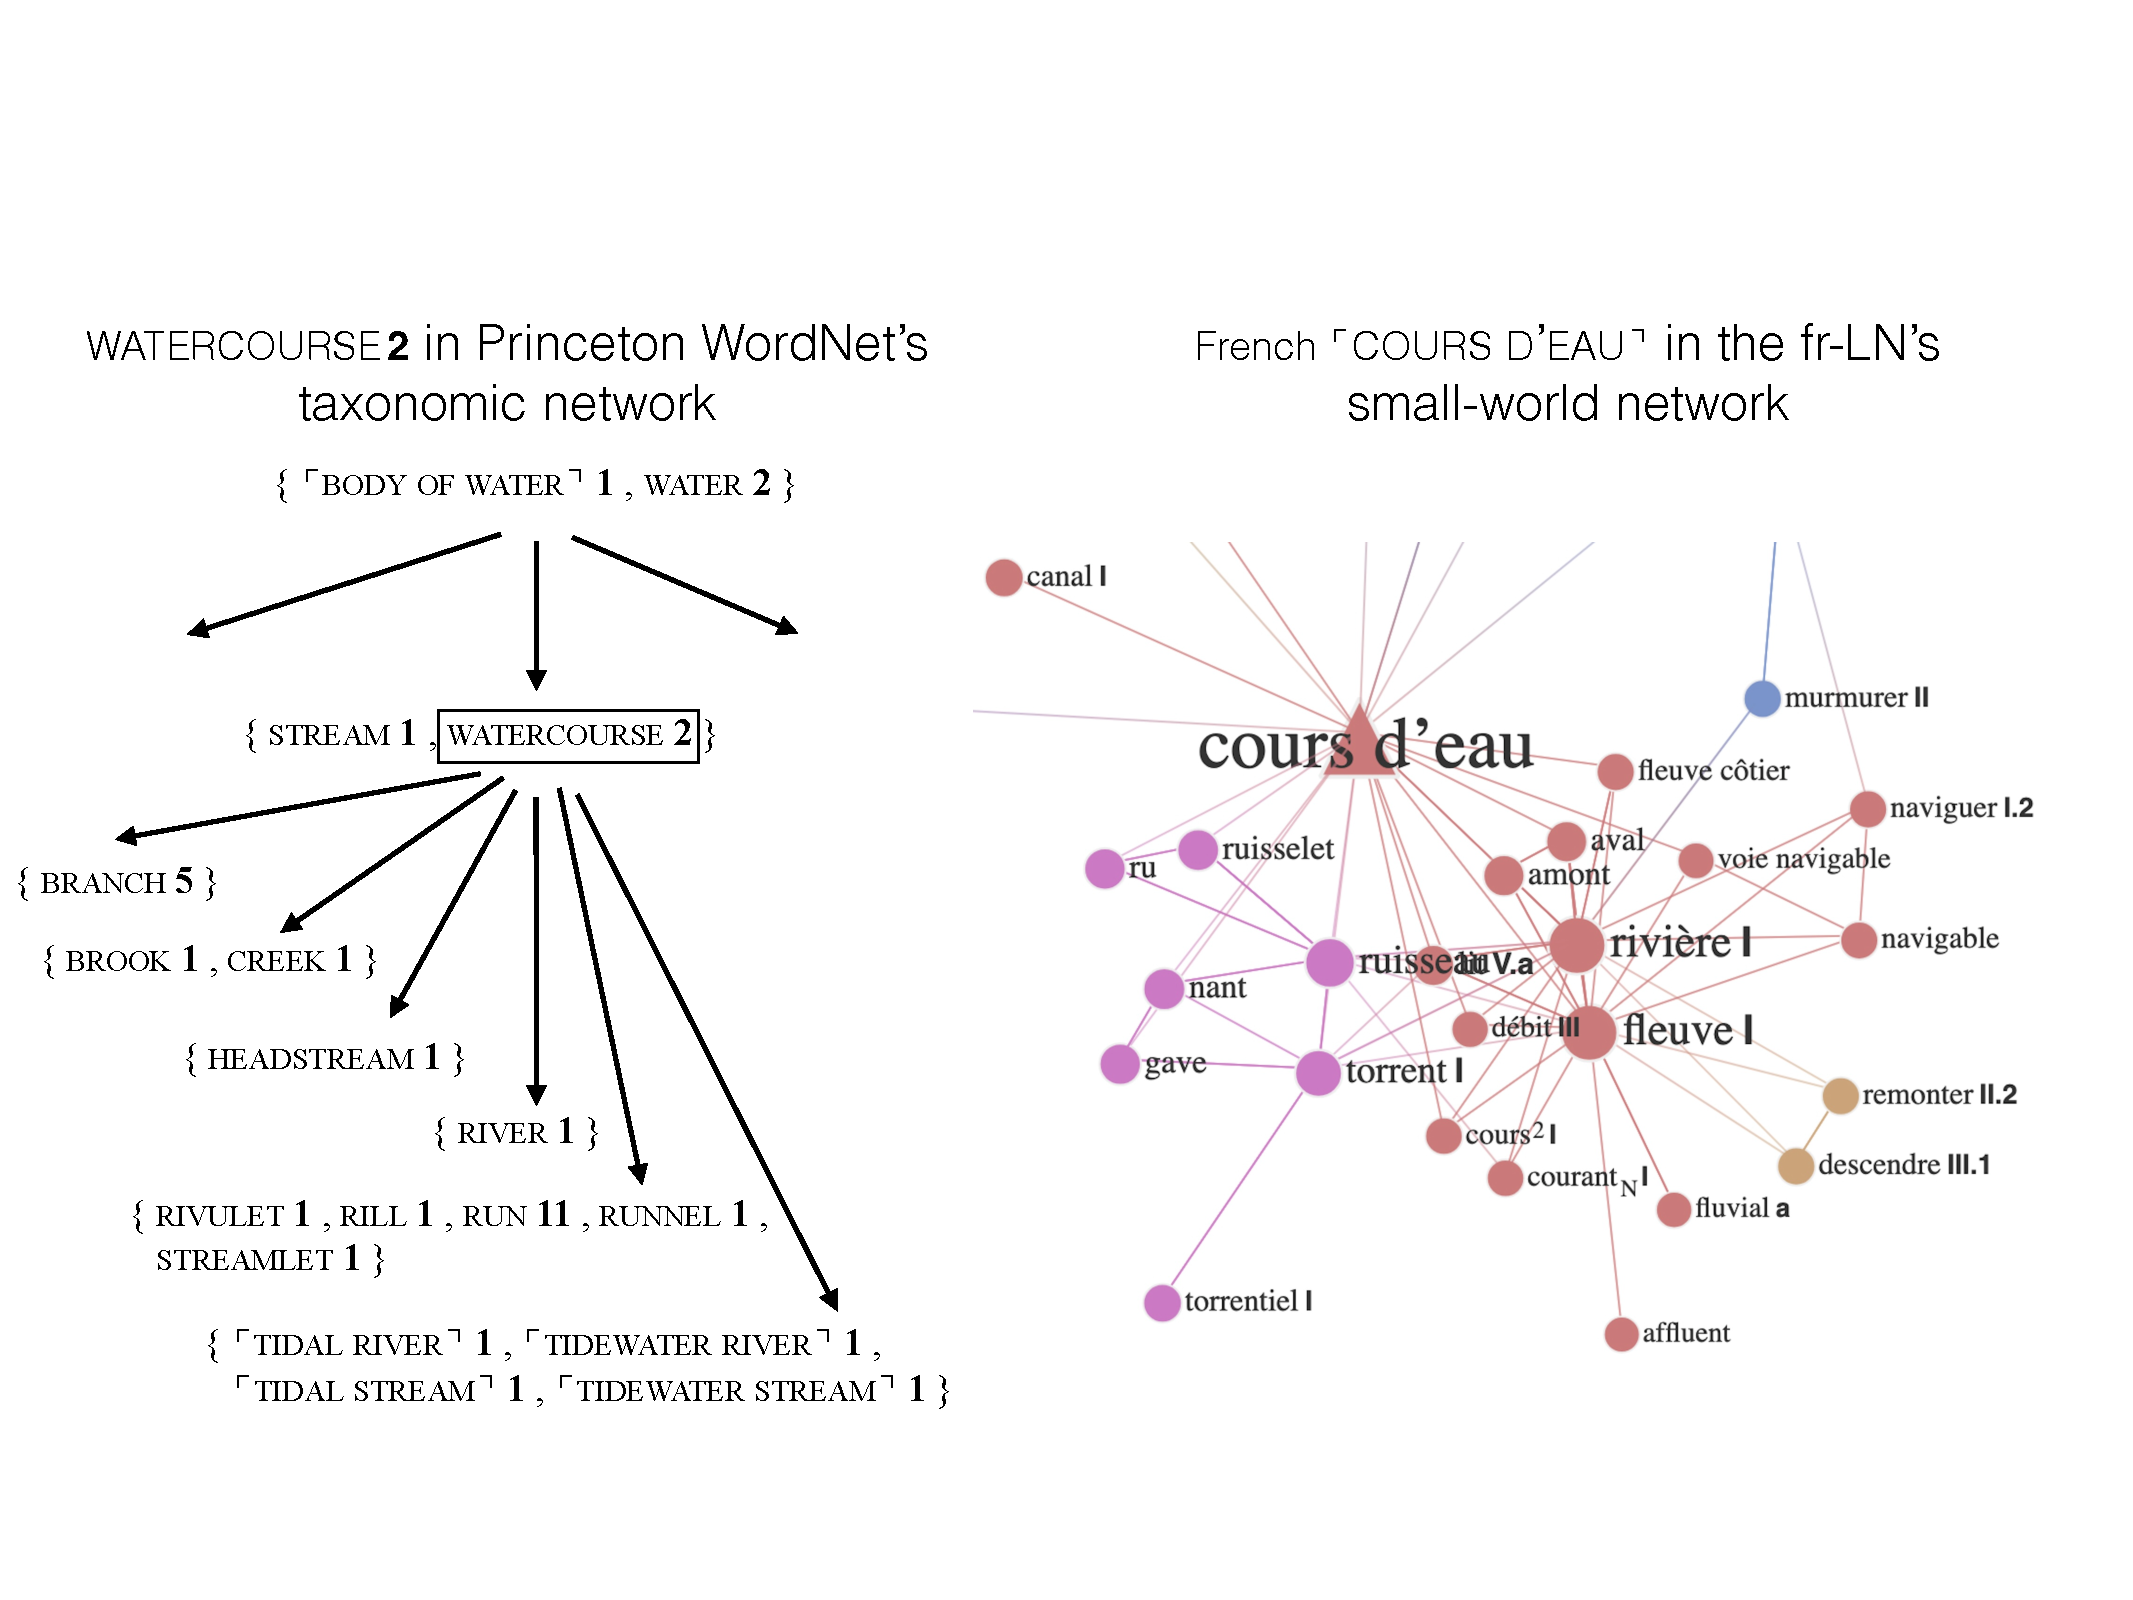
\includegraphics[width=0.97\linewidth]{Fig/LexicalNetworks/TaxonomicSmallworldLN.pdf}
\caption{Taxonomic vs. small-world lexical networks}\label{fig:taxonomicNonTaxonomicLNs}
\end{figure}

Though both the Princeton WordNet and the fr-LN have the ambition to reflect the organization of the Mental Lexicon, \figref{fig:taxonomicNonTaxonomicLNs} clearly shows how different structuring principles adopted for lexical network models induce different characteristic ``shapes'' of these models.\footnote{For arguments in favor of choosing small-world lexical networks over taxonomic ones, see \textcite{Polguere2014c-e} and \textcite{GotkovaEtAl2024}. The computable nature of small-world lexical networks as data structures is presented in \sectref{sec:formalPropertiesLS} (p.\thinspace\pageref{sec:formalPropertiesLS}).}\index[notion]{data structure}\index[notion]{structure!data \tld}

We present in \sectref{sec:LexicalSystems} (p.\thinspace\pageref{sec:LexicalSystems}) lexicon models called Lexical Systems\index[notion]{Lexical System}, of which the fr-LN is a particular instance, and highlight the fundamental role played by LF relations in such network lexicon models. Before we do that, let us briefly examine paradigmatic lexical relations encoded in WordNet from the perspective of LFs.

\paragraph*{WordNet's paradigmatic relations from the LF perspective.}\label{par:paraRelWordNet}

The taxonomic organization of WordNet -- illustrated in \figref{fig:taxonomicNonTaxonomicLNs} -- operates only in the nominal component of this lexical database\index[notion]{lexical database!WordNet}\index[notion]{WordNet!Princeton \tld} \parencite{Miller1990}, which is subdivided according to part of speech classification (nouns, verbs, adjectives and adverbs) and follows different structuring principles for each part of speech.

Furthermore, WordNet has a hybrid network structure where \textit{senses} themselves (and not only \textit{synsets}) can be connected. Such is the case for WordNet's so-called \textit{morphosemantic links}, which were grafted onto the original version of the database \parencite{MillerFellbaum2003}: they indicate lexical relations that would be encoded by us with paradigmatic LFs\index[notion]{lexical function!paradigmatic \tld}\index[notion]{paradigmatic!\tld\ lexical function}. In WordNet, these links are not typed, but identified under the same label: \texttt{derivation}, described as being a ``derivational morphology pointer.'' This is illustrated in \figref{fig:subnetworkWordNetMARRY-1}, which shows the WordNet subnetwork of \texttt{derivation} links extracted by taking the sense \textsc{marry}\sensenum{1} as point of origin and recursively following these links until all available \texttt{derivation} links are exhausted.\footnote{The present discussion is based on data extracted from version 3.1 of the Princeton WordNet.}

In order to clarify the nature of WordNet senses appearing in \figref{fig:subnetworkWordNetMARRY-1}, we list in 	\tabref{tab:ExtractWNPolysemyMARRY} their definitions in WordNet -- called \textit{glosses}\index[notion]{gloss in WordNet}\index[notion]{WordNet!gloss of a \tld\ sense} \parencite[240]{MillerEtAl1990} -- together with the relevant neighboring polysemy\index[notion]{polysemy}.

\begin{figure}

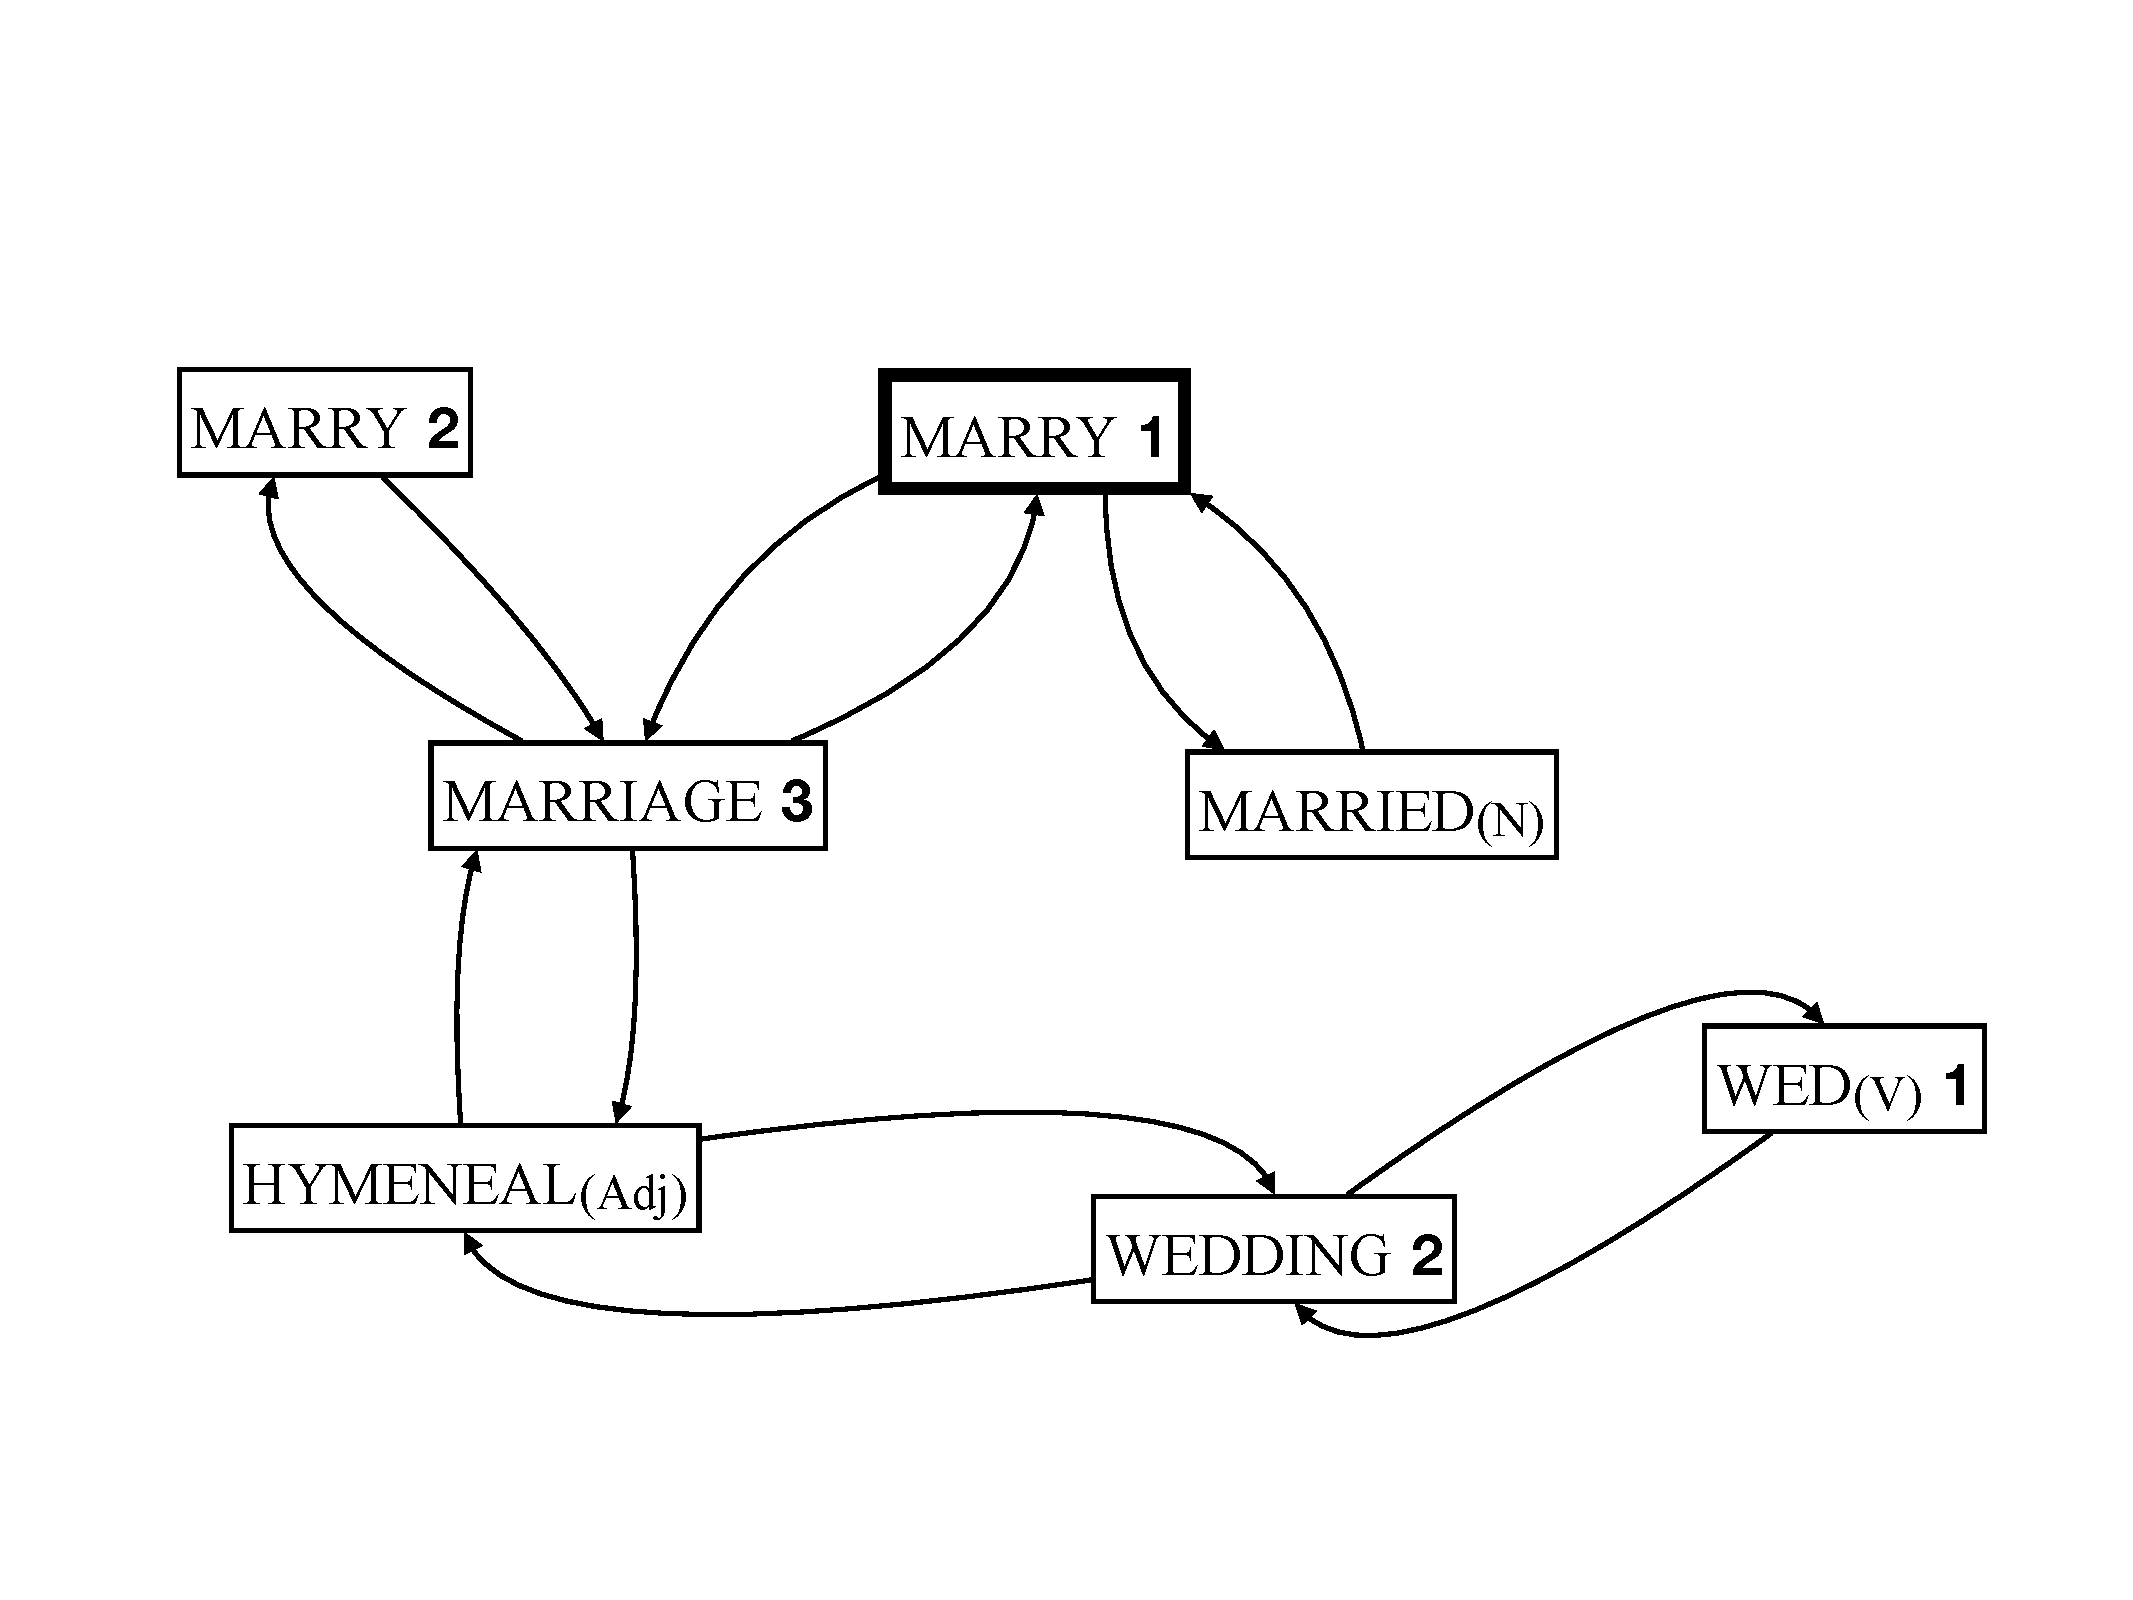
\includegraphics[width=.53\linewidth]{Fig/LexicalNetworks/subnetworkWordNetMARRY-1.pdf}
\caption{Subnetwork of \texttt{derivation} links in WordNet originating from \textsc{marry}\sensenum{1}}\label{fig:subnetworkWordNetMARRY-1}
\end{figure}

\begin{table}

\footnotesize
\renewcommand*{\arraystretch}{1}
\setlength{\tabcolsep}{4pt}
\begin{tabular}{ >{\raggedright\arraybackslash}p{.15\linewidth}  >{\raggedright\arraybackslash}p{.80\linewidth} }
\lsptoprule

\textsf{Senses}
& \textsf{Glosses} \\
\midrule

\lu{marry}{}{}{1}
& \textit{take in marriage} \\
\lu{marry}{}{}{2}
& \textit{perform a marriage ceremony} \\

\midrule

\lu{marriage}{}{}{1}
& \textit{the state of being a married couple voluntarily joined for life (or until divorce)} \\
\lu{marriage}{}{}{2}
& \textit{two people who are married to each other} \\
\lu{marriage}{}{}{3}
& \textit{the act of marrying; the nuptial ceremony} \\

\midrule

\lu{married}{(N)}{}{}
& \textit{a person who is married} \\

\midrule

\lu{hymeneal}{(Adj)}{}{}
& \textit{of or relating to a wedding or marriage} \\

\midrule

\lu{wedding}{}{}{1}
& \textit{the social event at which the ceremony of marriage is performed} \\
\lu{wedding}{}{}{2}
& same gloss as its synonym \lu{marriage}{}{}{3}: it belongs to the same synset (WordNet's glosses are associated to synsets, not to individual senses) \\

\midrule

\lu{wed}{(V)}{}{1}
& same gloss as its synonym \lu{marry}{}{}{1} \\
\lu{wed}{(V)}{}{2}
& same gloss as its synonym \lu{marry}{}{}{2} \\

\lspbottomrule
\end{tabular}\caption{Extract of WordNet's polysemy around the vocable \textsc{marry}}\label{tab:ExtractWNPolysemyMARRY}
\end{table}

Let us make three comments about \figref{fig:subnetworkWordNetMARRY-1}, taking the perspective of the encoding of paradigmatic relations by means of LFs.

\begin{enumerate}

\item WordNet's \texttt{derivation} links encode a very heterogeneous set of paradigmatic relations that can be discriminated with LFs; e.g., in \figref{fig:subnetworkWordNetMARRY-1}:

\begingroup
\small

\ex. \begingroup\setlength{\tabcolsep}{2pt}
\begin{tabular}[t]{ >{\raggedright\arraybackslash}p{2cm} >{\raggedright\arraybackslash}p{2cm} >{\raggedright\arraybackslash}p{6cm} }
\lu{marry}{}{}{1} & \lexRel{\lf{S\tsub{0}}} & \lu{marriage}{}{}{3}\\
\lu{marriage}{}{}{3} & \lexRel{\lf{V\tsub{0}}} & \lu{marry}{}{}{1}\\
\lu{marry}{}{}{1} & \lexRel{\lf{S\tsub{1/2}Perf}} & \lu{married}{(N)}{}{}\\
\end{tabular}\endgroup

\endgroup

This is a known issue with \texttt{derivation} links in WordNet. For a proposal to improve the description, see \textcite{FellbaumEtAl2009}.

\item A \texttt{derivation} link does not necessarily encode a morphological derivation\index[notion]{morphology!morphological derivative}\index[notion]{derivative!morphological \tld}, in spite of being termed \textit{morphosemantic} in the WordNet literature. Such is the case of the link between \lu{marriage}{}{}{3} and \lu{hymeneal}{(Adj)}{}{} in \figref{fig:subnetworkWordNetMARRY-1}: a case of \lf{A\tsub{0}}, in terms of LFs. Because morphology is not necessarily involved, these links can be considered as encoding \emph{semantic} derivations\index[notion]{semantic!\tld\ derivative}\index[notion]{derivative!semantic \tld}, just like paradigmatic LFs.

\item The encoding of semantic derivations in WordNet can be implemented in surprising ways. For instance, the absence of \textsc{spouse} in \figref{fig:subnetworkWordNetMARRY-1} is somehow strange, given the presence of the very marginal term \textsc{married}\tsub{(N)}. The noun \textsc{spouse} happens to be connected to \lu{marriage}{}{}{2} -- not \lu{marriage}{}{}{3} -- by the WordNet relation of meronymy\index[notion]{meronymy}. Because \lu{marriage}{}{}{2} is glossed as denoting a set of two persons rather than a social relation between two individuals (cf. 	\tabref{tab:ExtractWNPolysemyMARRY}),\footnote{WordNet illustrates this sense with the following example: \textit{his second marriage was happier than the first}.} \textsc{spouse} is modeled as denoting a unit of a marriage\sensenum{2} and therefore does not surface in \figref{fig:subnetworkWordNetMARRY-1}.

\end{enumerate}

This last observation illustrates the importance of organizing the modeling of paradigmatic -- and syntagmatic! -- relations by means of a coherent, well-defined \emph{system} of such relations that guides the process of exploring -- not just encoding -- lexical relations.

\section{Lexical Systems as network lexicon models}\label{sec:LexicalSystems}

A \notion{Lexical System}\index[notion]{Lexical System|emph} \parencite{Polguere2009-e,Polguere2014c-e} -- with capitalized initials -- is a lexicon model structured as a network of lexical entities connected, primarily, by paradigmatic and syntagmatic LF relations. Though built according to the principles of Explanatory Combinatorial Lexicology\index[notion]{Explanatory Combinatorial!\tld\ Lexicology}\index[notion]{lexicology!Explanatory Combinatorial \tld}, Lexical Systems have a formal structure radically different from that of Explanatory Combinatorial Dictionaries\index[notion]{Explanatory Combinatorial!\tld\ Dictionary}\index[notion]{dictionary!Explanatory Combinatorial \tld} \parencite{MelcukZholkovsky1984,MelcukZolkovskij2016,MelcukEtAl1984,MelcukEtAl1988,MelcukEtAl1992,MelcukEtAl1999}, these latter being textual (therefore, linear) representations of lexical knowledge\index[notion]{lexical knowledge}.

This section contains two parts: main characteristics of Lexical Systems (\sectref{sec:mainCharacteristicsLS}) and formal properties of Lexical Systems (\sectref{sec:formalPropertiesLS}).

The Lexical System approach has been applied to the construction of several lexical networks (LNs), in particular, for French (fr-LN)\index[notion]{French Lexical Network [fr-LN]}\index[notion]{lexical network!French \tld\ [fr-LN]}\index[notion]{lexical database!French Lexical Network [fr-LN]}, English (en-LN)\index[notion]{English Lexical Network [en-LN]}\index[notion]{lexical network!English \tld\ [en-LN]}\index[notion]{lexical database!English Lexical Network [en-LN]} and Russian (ru-LN)\index[notion]{Russian Lexical Network [ru-LN]}\index[notion]{lexical network!Russian \tld\ [ru-LN]}\index[notion]{lexical database!Russian Lexical Network [ru-LN]}. Because at the present time only the fr-LN (\sectref{sec:fr-LN}) can be considered as being a full-fledged Lexical System, our illustrations are mostly borrowed from this particular lexical database.\footnote{For information on exploratory lexicographic work conducted on the en-LN, see \textcite{GaderEtAl2014a-e}; on the ru-LN, see \textcite{Krylosova2017-e} and \textcite{Mikhel2022b}.}

\subsection{Main characteristics of Lexical Systems}\label{sec:mainCharacteristicsLS}

\subsubsection{LF relations: the backbone of Lexical Systems}\label{sec:LFRelationsBackboneOfLFs}

Going back to Postulate~1 (the network structure of lexicons: \sectref{sec:shapeOfLexicons}, p.\thinspace\pageref{txt:postulateStrucLexicons}), we can characterize Lexical Systems as information structures made up of two types of elements:

\begin{enumerate}

\item lexical entities\index[notion]{lexical entity}, as defined in Chapter~\ref{chap:preliminaryNotions} (\sectref{sec:lexicalNotions}, p.\thinspace\pageref{txt:lexicalEntityDef}) -- primarily, lexical units, but also, compositional phrasemes\index[notion]{phraseme!compositional \tld}\footnote{I.e., collocations and (linguistic) clichés. An illustration of a lexical entity of the fr-LN that is a linguistic cliché can be found in \figref{fig:proxemyCIGARETTE} (\sectref{sec:lexicalProximityTopologicalProximity}, p.\thinspace\pageref{fig:proxemyCIGARETTE}): {\smaller French}~\textit{Fumer tue} `Smoking kills' (bottom left corner of the figure). This cliché is a pragmateme \parencite{Melcuk2020a} used as a warning to smokers, written on packs of cigarettes.}\index[notion]{collocation}\index[notion]{cliche@clich\'e, linguistic}\index[notion]{pragmateme} and word-formation means analogous to lexemes;

\item lexical relations\index[notion]{lexical relation}\index[notion]{relation!lexical \tld} that connect these entities, as defined in Chapter~\ref{chap:NotionLF} (\sectref{sec:FLStandard2Carac}, p.\thinspace\pageref{txt:lexicalRelationIntro}) -- primarily, LF relations (other relations that play an important structuring role in Lexical Systems are presented in \sectref{sec:non-LFRelationsInLSs}, p.\thinspace\pageref{sec:non-LFRelationsInLSs}).

\end{enumerate}

Elements of the first type correspond to the \notion{nodes}\index[notion]{node of a network\slashs{}graph|emph}\index[notion]{network \lfgp{see also \textit{graph}}!node of a \tld|emph} of the lexical network and elements of the second type correspond to the \notion{arcs}\index[notion]{arc of a network\slashs{}graph|emph}\index[notion]{network \lfgp{see also \textit{graph}}!arc of a \tld|emph} of the network. \figref{fig:canal-coursDEau} illustrates these two notions. It is a blow-up of a segment of the fr-LN's subnetwork given in \figref{fig:taxonomicNonTaxonomicLNs} (p.\thinspace\pageref{fig:taxonomicNonTaxonomicLNs}) that features two lexical nodes -- {\smaller French}~\textsc{canal}\sensenum{I}  {\small `\lfgp{water} canal'} and \idiom{\textsc{cours d'eau}} {\small `watercourse'}, which are connected by an arc corresponding to the LF relation \lf{Gener}\index[lf]{Gener@\lf{Gener}}; i.e., in terms of LF application\index[notion]{application of an LF}\index[notion]{lexical function!application of a \tld}, it encodes \lfappl{Gener}{\textit{canal}\sensenum{I}} = \idiom{\textit{cours d'eau}}. In the pop-up of \figref{fig:canal-coursDEau}, ``\uslabel{FL}'' stands for {\smaller French}~\textit{fonction lexicale}.

As a rule, an LF application \lfappl{f}{L} translates within a Lexical System as a set of arcs labeled with the LF \lf{f} that originate from the lexical node L and lead to each individual value\index[notion]{lexical function!value of a \tld}\index[notion]{value of an LF} elements of the LF application. They are called \notion{outgoing arcs}\index[notion]{arc of a network\slashs{}graph!outgoing \tld|emph}, relative to L, and \notion{incoming arcs}\index[notion]{arc of a network\slashs{}graph!incoming \tld|emph}, relative to these elements.

\begin{figure}

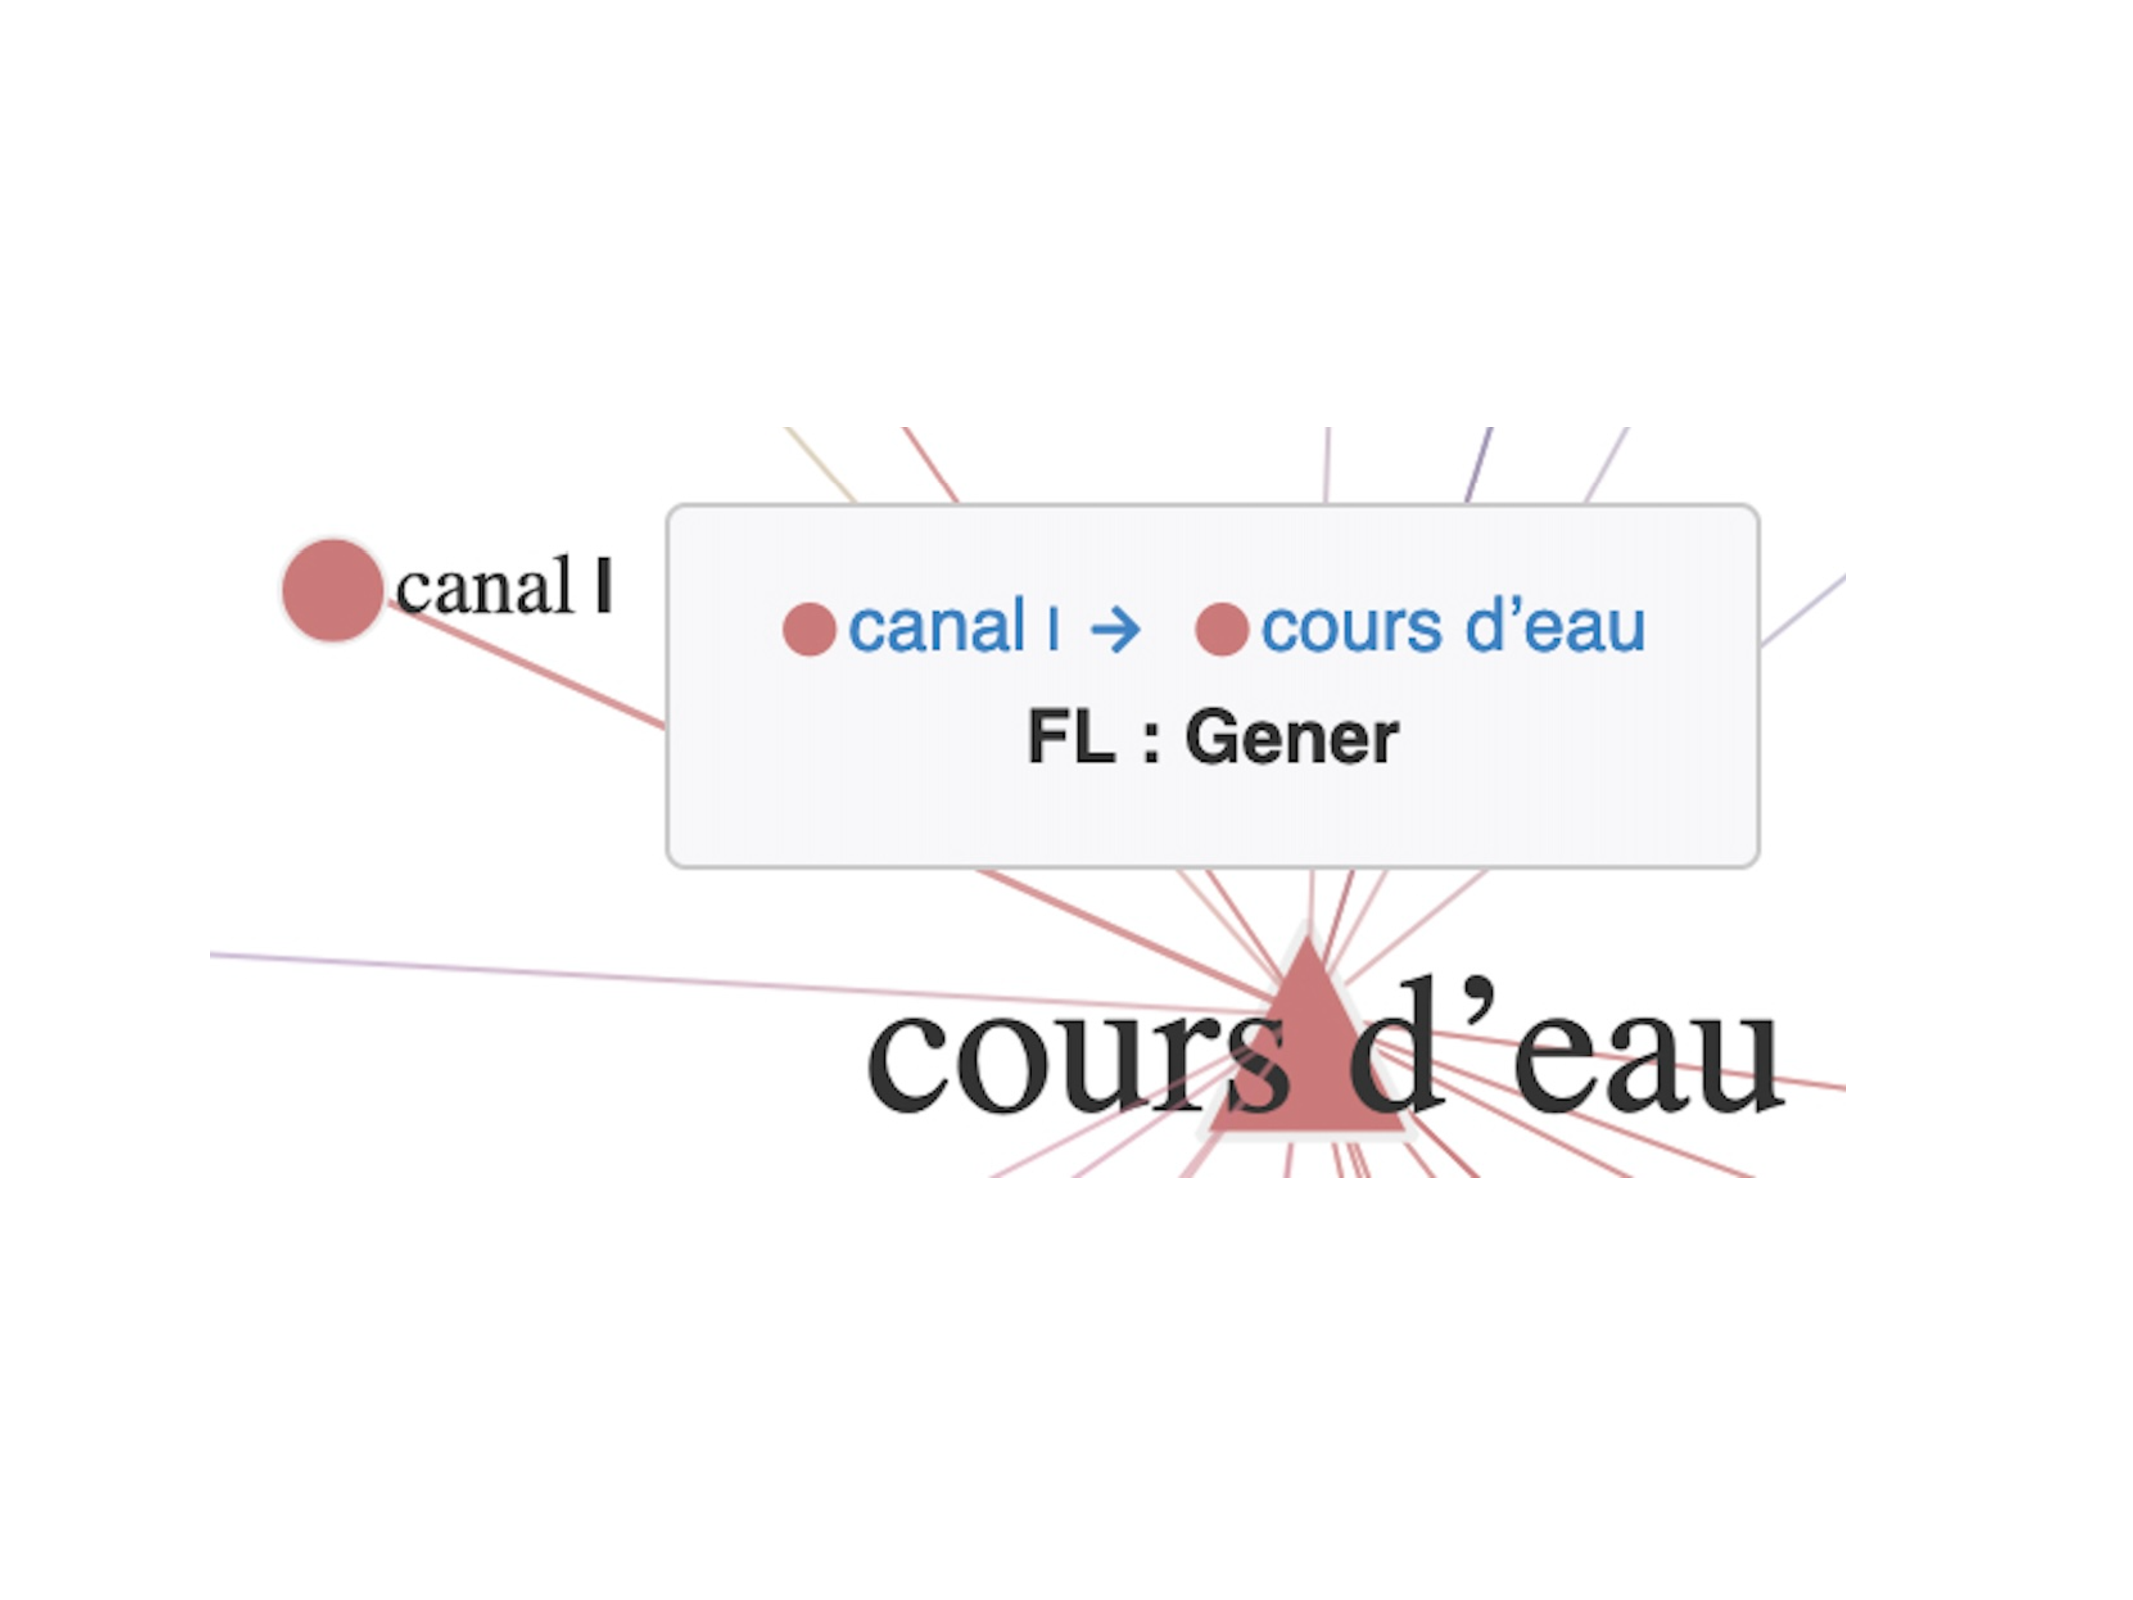
\epsfig{width=4cm,file=Fig/LexicalNetworks/canal-coursDEau.pdf}
\caption[\lfappl{Gener}{\textit{canal}\sensenum{I} {\footnotesize `\lfgp{water} canal'}} = \idiom{\textit{cours d'eau}} {\footnotesize `watercourse'} as represented in the fr-LN]{LF application \lfappl{Gener}{\textit{canal}\sensenum{I} {\footnotesize `\lfgp{water} canal'}} = \idiom{\textit{cours d'eau}} {\footnotesize `watercourse'} as represented in the fr-LN}\label{fig:canal-coursDEau}
\end{figure}

\phantomsection\label{rem:visualizationLS}\begin{soundbox}{Visualization of Lexical Systems}\index[notion]{visualization}
In the present chapter, we make use of a dedicated \notion{network browser}\index[notion]{network \lfgp{see also \textit{graph}}!\tld\ browser}, called \notion{Spiderlex}\index[notion]{Spiderlex|emph}, for the visualization of the content of Lexical Systems \parencite{OllingerEtAl2020,OllingerPolguere2020b-e}. Spiderlex exploits the mathematical properties of the small-world\index[notion]{small-world!\tld\ network}\index[notion]{network \lfgp{see also \textit{graph}}!small-world \tld}\index[notion]{lexical network} structure of Lexical Systems (\sectref{sec:formalPropertiesLS}, p.\thinspace\pageref{sec:formalPropertiesLS}) and plays an important role for the utilization of lexical data both by lexicographers and users of the fr-LN -- see \sectref{sec:lexicographyOfLNs}, p.\thinspace\pageref{sec:lexicographyOfLNs}. Note that the orientation of arcs\index[notion]{arc of a network\slashs{}graph!orientation of an \tld}\index[notion]{orientation of a network arc} and their labels\index[notion]{arc of a network\slashs{}graph!label of an \tld}\index[notion]{label of a network\slashs{}graph arc} are not displayed by default, as in \figref{fig:taxonomicNonTaxonomicLNs}, in order to keep the visualization legible; this information can be shown by pointing at individual arcs, as in \figref{fig:canal-coursDEau}.\footnotemark
\end{soundbox}\footnotetext{\label{fn:fr-LNDataEvolving}Data from the fr-LN used in this chapter and the screenshots from Spiderlex reflect the state of this constantly evolving model at time of writing.}

The notion of Lexical System, first introduced in \textcite{Polguere2009-e}, gradually took shape out of the practice of computational Explanatory Combinatorial Lexicography\index[notion]{lexicography!computational Explanatory Combinatorial \tld}\index[notion]{Explanatory Combinatorial!computational \tld\ Lexicography} \parencite{Steinlinetal2005,PolguereMelcuk2006}. It was based on the observation that the system of simple standard LFs\index[notion]{system of standard LFs}\index[notion]{lexical function!system of standard \tlds} -- in particular LFs identified in this book as being central\index[notion]{lexical function!central \tld\ (in the system of standard \tlds)} (\chapref{chap:NotionLF}, \sectref{sec:centralLFs}, p.\thinspace\pageref{sec:centralLFs}) -- was a good candidate as main contributor to the structuring of lexical knowledge\index[notion]{lexical knowledge}, better by all means than mainstream taxonomic\index[notion]{taxonomy} principles. This has lead to a second postulate, this time concerning the structure of Lexical Systems.

\phantomsection\label{txt:postulateStrucLS}\begin{soundbox}{Postulate 2: structure of Lexical Systems}
Lexical Systems, as network lexicon models, are primarily structured by standard LF relations.
\end{soundbox}

Postulate~2 implies that LF relations form the backbone of Lexical Systems. From a methodological viewpoint, the lexicographic\index[notion]{lexicography!\tld\ of lexical networks}\index[notion]{lexical network!lexicography of \tlds} process of building a Lexical System for a given natural language is driven by the weaving of standard LF relations within the lexical network \parencite{LuxPogodallaPolguere2011,Polguere2012e-e}.

Two properties of standard LFs can be put forward in support of the adoption of Postulate~2:

\begin{enumerate}

\item Standard LFs express constrained meanings (\chapref{chap:NotionLF}, \pageref{sec:LFDefinitionNotion}, p.\thinspace\pageref{txt:constrainedMeaning})\index[notion]{meaning!constrained \tld}, present in all natural languages; these meanings determine fundamental paradigmatic and syntagmatic relations between lexical units.

\item A standard LF is essentially related to the meaning of each individual lexical unit L it takes as argument, in the sense that it is anchored in L's definition\index[notion]{definition!lexicographic \tld} -- cf. the notion of LF target\index[notion]{lexical function!target of a \tld}\index[notion]{target of an LF} (\chapref{chap:NotionLF}, \sectref{sec:classeFLSyntagmatiques}, p.\thinspace\pageref{txt:targetOfSyntLF}). Conversely, a standard LF can serve as a revealer of the presence of a particular semantic chunk in L's meaning \parencite{IordanskajaPolguere2005}.

\end{enumerate}

\paragraph*{Relational profile of a node\slashs{}lexical unit.}\label{par:relationalProfile}

Because of the above properties, it is justified to consider that each node\index[notion]{node of a network\slashs{}graph}\index[notion]{network \lfgp{see also \textit{graph}}!node of a \tld} \textit{n} of a Lexical System -- and the corresponding lexical unit L -- has a \notion{relational profile}\index[notion]{relational profile|emph}\index[notion]{profile, relational|emph} consisting of two sets: the set of \textit{n}'s outgoing arcs and the set of its incoming arcs.

\begin{itemize}

\item The set of \textit{n}'s outgoing arcs\index[notion]{arc of a network\slashs{}graph!outgoing \tld}\index[notion]{network \lfgp{see also \textit{graph}}!arc of a \tld} -- i.e., L's \notion{outgoing profile}\index[notion]{relational profile!outgoing \tld}\index[notion]{profile, relational!outgoing \tld} -- is the main constituent of L's relational profile as it is a reflection of the essential semantic and combinatorial properties of L. It corresponds to the information listed in the cooccurrence zone\index[notion]{lexical entry!cooccurence zone of a \tld}\index[notion]{zone of a lexical entry!cooccurrence \tld} in an Explanatory Combinatorial Dictionary\index[notion]{Explanatory Combinatorial!\tld\ Dictionary}\index[notion]{dictionary!Explanatory Combinatorial \tld} -- see Appendix, p.\thinspace\pageref{sec:AppendixLFZone}.

\item The set of \textit{n}'s incoming arcs\index[notion]{arc of a network\slashs{}graph!incoming \tld} -- i.e., L's \notion{incoming profile}\index[notion]{relational profile!incoming \tld}\index[notion]{profile, relational!incoming \tld} -- is a relational information that is \emph{not} present in the cooccurrence zone of L's lexical entry in an Explanatory Combinatorial Dictionary\index[notion]{Explanatory Combinatorial!\tld\ Dictionary}\index[notion]{dictionary!Explanatory Combinatorial \tld} and, more importantly, that is simply not encoded in this type of model. In a Lexical System, by contrast, incoming profiles are embedded in the model's network structure and can be accessed directly.

\end{itemize}

This is illustrated in	\figref{fig:outgoingIncomingProfile}, with an adaptation of the Spiderlex\index[notion]{Spiderlex} visualization\index[notion]{visualization} of both the current outgoing and incoming profiles of {\smaller French}~\textsc{sentiment}\sensenum{1a} `feeling' in the fr-LN. The complementarity of the two profiles is well illustrated by the contrast between the unique outgoing \lf{Gener}\index[lf]{Gener@\lf{Gener}} relation (towards {\smaller French}~\textit{état psychique} `psychological state') and the large set of incoming \lf{Gener} relations, which characterizes {\smaller French}~\textsc{sentiment}\sensenum{1a} as being a generic term\index[notion]{generic term} (i.e., classifying lexical unit) in the French lexicon\index[notion]{noun!\tld\ of feeling}.

\begin{figure}

\scriptsize
\setlength{\tabcolsep}{1pt}
\setlength\extrarowheight{1.2pt}
\APolbox{5.3cm}{%
\begin{tabular}{ l c >{\raggedright\arraybackslash}p{3.4cm} }
\multicolumn{3}{ c }{{\small \textsf{Outgoing LF relations}}} \\[+4pt]
\lf{Syn$_\supset$}
& :
& \textit{émotion}\sensenum{2} \\
\lf{Syn$_\cap$}
& :
& \textit{sensation}\sensenum{1}\textbf{,}  \uslabel{spec} \textit{affect}\sensenum{a}\textbf{;} \uslabel{spec} \textit{état émotionnel} \\
\lf{Gener}
& :
& \uslabel{(spec)} \textit{état psychique} \\
\lf{S$_\text{loc}^\text{prototyp}$}
& :
& \textit{cœur}\sensenum{III.1}\textbf{;} \textit{âme}\sensenum{I}\textbf{,} \textit{esprit}\sensenum{I.1} \\
\lf{Magn}
& :
& \textit{vif}\sensenum{II.2}\textbf{,} \textit{profond}\tsub{(Adj)}\sensenum{II}\textbf{,} \textit{fort}\tsub{(Adj)}\sensenum{III.2} \\
\lf{Oper\tsub{1}}
& :
& \textit{éprouver}\sensenum{a} \lfgp{\textsc{art} \tld}\textbf{,}  \textit{ressentir} \lfgp{\textsc{art}~\tld}\textbf{;} \textit{nourrir}\sensenum{II.1} \lfgp{\textsc{art} \tld}\textbf{,} \textit{avoir}\sensenum{VII.2} \lfgp{\textsc{art} \tld} \\
\lf{Func\tsub{1}}
& :
& \textit{habiter}\sensenum{II} \lfgp{N\tsub{X}} \textbf{<} \textit{étreindre}\sensenum{II} \lfgp{N\tsub{X}} \textbf{<} \textit{submerger}\sensenum{II} \lfgp{N\tsub{X}} \\
\lf{IncepFunc\tsub{1}}
& :
& \textit{naître}\sensenum{II} \lfgp{\textit{en} N\tsub{X}}\textbf{,} \textit{envahir}\sensenum{III} \lfgp{N\tsub{X}}\textbf{,} \textit{saisir}\sensenum{III} \lfgp{N\tsub{X}}\textbf{,}  \textit{prendre}\sensenum{VIII} \lfgp{N\tsub{X}} \textbf{<} \textit{s'emparer}\sensenum{II.2} \lfgp{\textit{de} N\tsub{X}} \\
\lf{Caus\tsub{1}Func\tsub{2'}}
& :
& \textit{transférer}\sensenum{III} \lfgp{\textsc{art} \tld\ \textit{sur} N\tsub{Y'}} \\
\lf{Fact\tsub{1}}
& :
& \textit{guider}\sensenum{II} \lfgp{N\tsub{X}}\textbf{,} \textit{animer}\sensenum{III} \lfgp{N\tsub{X}} \\
\lf{IncepManif}
& :
& \textit{se peindre} \lfgp{\textit{sur} N} \\
\multicolumn{3}{c}{} \\[59pt]
\end{tabular}
}
\hphantom{.}
\APolbox{6.6cm}{%
\begin{tabular}{ l c >{\raggedright\arraybackslash}p{5cm} }

\multicolumn{3}{ c }{{\small \textsf{Incoming LF relations}}} \\[+4pt]

\lf{Syn$_\subset$}
& \textsf{\textbf{for}}
& \textit{émotion}\sensenum{2} \\

\lf{Syn$_\cap$}
& \textsf{\textbf{for}}
& \textit{affect}\sensenum{a}\thinspace-- \textit{état émotionnel}\thinspace-- \textit{sensation}\sensenum{1} \\

\lf{Gener}
& \textsf{\textbf{for}}
& \textit{admiration}\thinspace-- \textit{allégresse}\thinspace-- \textit{amour}\sensenum{I.1a}\thinspace-- \textit{amour}\sensenum{I.1b}\thinspace-- \textit{animosité}\sensenum{1}\thinspace-- \textit{appitoiement}\sensenum{a}\thinspace-- \textit{appitoiement}\sensenum{b}\thinspace-- \textit{aversion}\thinspace-- \textit{bonheur}\sensenum{1}\thinspace-- \textit{cafard}\sensenum{II}\thinspace-- \wf{chagrin}{(N)}{1}{1}\thinspace-- \textit{colère}\sensenum{1}\thinspace-- \textit{compassion}-- \textit{contentement}\thinspace-- \textit{curiosité}\sensenum{I.2}\thinspace-- \textit{déception}\thinspace-- \textit{dégoût}\sensenum{II}\thinspace-- \textit{déprime}\thinspace-- \textit{désespoir}\sensenum{1}\thinspace-- \textit{désir}\sensenum{1}\thinspace-- \textit{désir}\sensenum{2}\thinspace-- \textit{dévastation}\sensenum{II.2}\thinspace-- \textit{doute}\thinspace-- \textit{effroi}\thinspace-- \textit{émoi}\thinspace-- \textit{émotion}\sensenum{1}\thinspace-- \textit{empathie}\thinspace-- \textit{étonnement}\thinspace-- \textit{fierté}\sensenum{I.1}\thinspace-- \textit{frayeur}\thinspace-- \idiom{\textit{froid dans le dos}}\thinspace-- \textit{frousse}\thinspace-- \textit{frustration}\thinspace-- \textit{fureur}\sensenum{I}\thinspace-- \textit{gratitude}\thinspace-- \textit{haine}\sensenum{1}\thinspace-- \textit{haine}\sensenum{2}\thinspace-- \textit{honte}\sensenum{I.1}\thinspace-- \textit{horreur}\sensenum{I}\thinspace-- \textit{horreur}\sensenum{II}\thinspace-- \textit{humiliation}\sensenum{2}\thinspace-- \textit{jalousie}\sensenum{I}\thinspace-- \idiom{\textit{mal au cœur}}\sensenum{II}\thinspace-- \idiom{\textit{mal du pays}}\thinspace-- \textit{malaise}\sensenum{3}\thinspace-- \textit{mécontentement}\thinspace-- \textit{mélancolie}\sensenum{II.1}\thinspace-- \textit{mépris}\thinspace-- \textit{nausée}\sensenum{II}\thinspace-- \textit{nostalgie}\sensenum{I}\thinspace-- \textit{orgueil}\sensenum{2a}\thinspace-- \textit{peur}\sensenum{1}\thinspace-- \textit{plaisir}\sensenum{I.1}\thinspace-- \textit{rage}\sensenum{II}\thinspace-- \textit{ravissement}\thinspace-- \textit{reconnaissance}\sensenum{II}\thinspace-- \textit{répugnance}\sensenum{1}\thinspace-- \textit{répulsion}\sensenum{I}\thinspace-- \textit{ressentiment}\thinspace-- \textit{satisfaction}\sensenum{II}\thinspace-- \textit{sentiment}\sensenum{1b}\thinspace-- \textit{souci}\sensenum{1}\thinspace-- \textit{spleen}\thinspace-- \textit{tristesse}\sensenum{I}\thinspace-- \textit{trouille}  \\


\lf{S$_\text{2}$}
& \textsf{\textbf{for}}
& \textit{éprouver}\sensenum{a} \\

\lf{S$_\text{2}^\text{prototyp}$}
& \textsf{\textbf{for}}
& \textit{émoji} \\

\lf{S$_\text{3}^\text{prototyp}$}
& \textsf{\textbf{for}}
& \textit{chantage}\sensenum{II} \\

\end{tabular}
}
\caption[Outgoing vs. incoming profiles of {\smaller French}~\textsc{sentiment}\sensenum{1a} `feeling' in the fr-LN]{Outgoing vs. incoming profiles of {\smaller French}~\textsc{sentiment}\sensenum{1a} `feeling' in the fr-LN}\label{fig:outgoingIncomingProfile}
\end{figure}

\figref{fig:outgoingIncomingProfile} shows that Lexical Systems' data need not be visualized graphically. Textual, dictionary-like visualizations similar to lexical entries of a traditional dictionary can also be generated from the same data. For this reason, the construction of Lexical Systems is presented in \textcite{Polguere2012d-e} as being a \notion{lexicography of virtual dictionaries}.\index[notion]{visualization!textual \tld}\index[notion]{lexical entry!automatically generated \tld}\index[notion]{dictionary!virtual \tld}\index[notion]{lexicography!\tld\ of virtual dictionaries}

Incoming profiles can play an important role in applications of lexical network models, for instance, in language teaching\index[notion]{teaching\slashs{}learning, language}\index[notion]{language teaching\slashs{}learning}. Thus, the meaning of the generic term\index[notion]{generic term} \textsc{precipitation}\sensenum{1} `type of weather condition'\footnote{The lexicographic number of \textsc{precipitation}\sensenum{1} comes from the LDOCE.}\index[notion]{dictionary!Longman Dictionary of Contemporary English@\textit{Longman Dictionary of Contemporary English} [LDOCE]}\index[notion]{Longman Dictionary of Contemporary English@\textit{Longman Dictionary of Contemporary English} [LDOCE]}\index[notion]{lexicographic number} is better taught to language learners by relying on this term's incoming profile, i.e., by listing some of the most typical lexical units for which \textsc{precipitation}\sensenum{1} is a \lf{Gener} -- \textsc{rain}\tsub{(N)}, \textsc{snow}\tsub{(N)}, \textsc{hail}\tsub{(N)}, etc. -- as most dictionaries do.\footnote{See, for instance, the largely enumerative definition of LDOCE: `any form of water, such as rain, snow, sleet, or hail, that falls to the Earth's surface'. On defining so-called \textit{functional collective superordinates} within the Natural Semantic Metalanguage approach, see \textcite{Goddard2017}.}\index[notion]{dictionary!Longman Dictionary of Contemporary English@\textit{Longman Dictionary of Contemporary English} [LDOCE]}\index[notion]{Longman Dictionary of Contemporary English@\textit{Longman Dictionary of Contemporary English} [LDOCE]}\index[notion]{definition!lexicographic \tld}\index[notion]{Natural Semantic Metalanguage} This is probably a better pedagogical strategy than trying to first provide learners with a lexicographic definition\index[notion]{definition!lexicographic \tld} that can only be non-specific and will be felt as more confusing than explanatory.

This observation does not necessarily apply to any generic terms, in particular to generic terms with more specific meanings, for which a lexicographic definition can be a good starting point in vocabulary teaching -- e.g., generic terms such as \textsc{bird}, \textsc{tree}\tsub{(N)}, etc. Collocative lexical units\index[notion]{lexical unit!collocative \tld} -- lexical units that are essentially selected by the Speaker\index[notion]{Speaker, the} as collocates\index[notion]{collocation!collocate of a \tld} in collocations -- are another illustration of the usefulness of incoming profiles. Thus, the intensifier \lu{heavy}{(Adj)}{}{2}\phantomsection\label{txt:HEAVY-Adj-2} \senseex{heavy rain}\footnote{The lexicographic number of \lu{heavy}{(Adj)}{}{2} comes from the LDOCE.}\index[notion]{dictionary!Longman Dictionary of Contemporary English@\textit{Longman Dictionary of Contemporary English} [LDOCE]}\index[notion]{Longman Dictionary of Contemporary English@\textit{Longman Dictionary of Contemporary English} [LDOCE]}\index[notion]{lexicographic number} controls very few outgoing LF relations and its relational profile resides essentially in all its incoming \lf{Magn}\index[lf]{Magn@\lf{Magn}} relations -- the set of all lexical units for which it is a \lf{Magn} (\textsc{accent}\tsub{(N)}, \textsc{accusation}, \textsc{applause}, \textsc{battle}\tsub{(N)}, \textsc{blow}\tsub{(N)}, \textsc{emphasis}, \textsc{fog}\tsub{(N)}, etc.). The meaning of \lu{heavy}{(Adj)}{}{2} is simply that of \lf{Magn} -- the same constrained meaning\index[notion]{meaning!constrained \tld} as for dozens of adjectival intensifiers in English; consequently, its incoming profile is as important as its definition in the acquisition\index[notion]{acquisition!lexical \tld} of this lexical unit by language learners.\footnote{It is interesting to contrast two types of dictionaries of collocations in the light of the notion of relational profile: (i) those whose entries are collocation bases and that provide the list of collocates they select -- see \textcite{BensonEtAl2010} for English and \textcite{Bosque2006} for Spanish; (ii)~those whose entries are collocates and that provide the list of corresponding bases in collocations -- see \textcite{Bosque2010} for Spanish. The former describe the outgoing relational profile of bases, while the latter describe the incoming relational profile of collocates.}\index[notion]{dictionary!\tld\ of collocations}\index[notion]{collocation!dictionary of \tlds}

\paragraph*{Semantic weight of LF relations.}\label{par:semanticWeightLFRelation}

All LF relations found in the relational profile of a given lexical unit L do not carry the same \notion{semantic weight}.\index[notion]{weight, semantic|emph}\index[notion]{semantic!\tld\ weight|emph}\footnote{The notion of semantic weight is further developed in \sectref{sec:formalPropertiesLS}, p.\thinspace\pageref{sec:formalPropertiesLS}.} Indeed, LFs are very diverse with respect to the semantic proximity they \emph{inherently} imply -- or not -- between their argument and their value. For instance, \lfappl{Syn}{L\tsub}\index[lf]{Syn@\lf{Syn}} = L′, \lfappl{V\tsub{0}}{L}\index[lf]{V0@\lf{V\tsub{0}}} = L′, \lfappl{A\tsub{1}}{L}\index[lf]{Ai@\lf{A\tsub{i}}!\lf{A\tsub{1}}} = L′, etc., obviously imply a strong \notion{meaning relation}\index[notion]{meaning!\tld\ relation|emph}\index[notion]{relation!meaning \tld|emph} between L and L′, as L′ is a semantic derivative\index[notion]{derivative!semantic \tld}\index[notion]{semantic!\tld\ derivative} of L. By contrast, \lfappl{Magn}{L}\index[lf]{Magn@\lf{Magn}} = L′, \lfappl{Loc\tsub{in}}{L}\index[lf]{Locin@\lf{Loc\tsub{in}}} = L′, \lfappl{Oper\tsub{1}}{L}\index[lf]{Operi@\lf{Oper\tsub{i}}!\lf{Oper\tsub{1}}}~= L′, etc., do not inherently imply any meaning relation between L and L′; such relation may exist ``incidentally,'' for a given case of \lfappl{f}{L} = L′, but not by virtue of the meaning \sigmaF\ of \lf{f} -- e.g., \lfappl{Magn}{\textit{appetite}} = \textit{ravenous} -- where \textit{appetite} means approximately `desire to eat' and \textit{ravenous}, when used freely (i.e., not as as an intensifier), means `who has a strong desire\slashs{}need to eat'.

In a Lexical System, each arc of the network that corresponds to an LF relation carries a semantic weight which is determined by the meaning \sigmaF\ of the corresponding LF \lf{f}. Prototypically, arcs corresponding to paradigmatic LFs (i.e., leading to semantic derivatives)\index[notion]{lexical function!paradigmatic vs. syntagmatic \tlds} tend to carry a stronger semantic weight than those corresponding to syntagmatic LFs. We will see shortly (\sectref{sec:non-LFRelationsInLSs}) that the notion of semantic weight also applies to non-LF relations.

Before proceeding with the examination of lexical relations in Lexical Systems that are not based on LFs, it is important to note that a given node \textit{n} of a Lexical System is a complex informational entity that encapsulates all the properties of the corresponding lexical unit L not accounted for by LF relations: grammatical characteristics, lexicographic definition\index[notion]{definition!lexicographic \tld}, etc. That is, the lexical properties specified in \textit{n} together with \textit{n}'s relational profile are informationally equivalent to a lexical entry\index[notion]{lexical entry} for L. Of course, in the context of the lexicography of lexical networks\index[notion]{lexicography!\tld\ of lexical networks}\index[notion]{lexical network!lexicography of \tlds} \parencite{Polguere2014c-e}, special lexicographic tools are required to construct individual nodes with their individual properties and to weave the relations between nodes (see \sectref{sec:lexicographyOfLNs}, p.\thinspace\pageref{sec:lexicographyOfLNs}).

\subsubsection{Non-LF relations between lexical units}\label{sec:non-LFRelationsInLSs}

Three non-LF relations\index[notion]{lexical relation!non-LF \tld} play an important role in Lexical Systems:

\begin{itemize}

\item copolysemy relation, holding between two lexical units of a polysemous vocable (\sectref{sec:copolysemyRelation});

\item idiom-component relation, holding between an idiom and a lexeme that participates in its surface-syntactic structure (\sectref{sec:idiomComponentRelation});

\item meaning-inclusion relation, holding between a lexical unit and another lexical unit that is an element of its lexicographic definition (\sectref{sec:meaningInclusionRelation}).

\end{itemize}

To make the presentation of these relations more straightforward and concrete, we base the following explanation mostly on data borrowed from the fr-LN.\index[notion]{French Lexical Network [fr-LN]}\index[notion]{lexical database!French Lexical Network [fr-LN]}\index[notion]{lexical network!French \tld\ [fr-LN]}

The order of presentation of the three non-LF relations is determined by the expertise that has been gained from lexicographic work on the fr-LN: from the most extensively described relations to those whose encoding is still at an experimental stage.

Finally, note that the relational profile\index[notion]{relational profile}\index[notion]{profile, relational} of a node\slashs{}lexical unit, while primarily based on LF relations, also includes the three relations that are presented below.

\subsubsubsection{Copolysemy relation}\label{sec:copolysemyRelation}

The fr-LN -- as should be the case of any full-fledged Lexical System -- contains the explicit modeling of the \notion{polysemy structure}\index[notion]{polysemy!\tld\ structure of a vocable|emph}\index[notion]{vocable!polysemy structure of a \tld|emph} of vocables through the encoding of so-called \notion{copolysemy relations}\index[notion]{polysemy!co\tld|emph}\index[notion]{copolysemy|emph}\index[notion]{lexical relation!copolosemy \tld|emph}\index[notion]{relation!copolysemy \tld|emph} between lexical units of a vocable. A copolysemy relation -- that is, the corresponding arc of the lexical network -- is oriented from the lexical unit that is the source of the ``copolysemy derivation'' toward the ``derived'' lexical unit. In other words, L\thinspace\lexRel{copolysemy}\thinspace{}L′ reads as `lexical unit L has lexical unit L′ as its copolysemy extension, metonymy, metaphor, ...'; this relation participates in the polysemy structure of a given vocable.

Some copolysemy relations have a strong semantic weight\index[notion]{semantic!\tld\ weight}\index[notion]{weight, semantic}\index[notion]{arc of a network\slashs{}graph!semantic weight of an \tld} in the network: they imply that the two lexical units they connect belong to identical semantic fields\index[notion]{semantic!\tld\ field}. This is the case of the metonymy\index[notion]{metonymy}\index[notion]{copolysemy!\tld\ relation of metonymy} relation that links {\smaller French}~\textsc{cigarette}\sensenum{I} `cigarette'\phantomsection\label{txt:CIGARETTE} to {\smaller French}~\textsc{cigarette}\sensenum{II} `habit of smoking \textit{cigarettes}\sensenum{I}'\footnote{Cf. \textit{Julie veut arrêter la cigarette} `Julie wants to stop smoking cigarettes'. There is no corresponding lexical unit in English. The polysemy of {\smaller French}~\textsc{cigarette} is chosen as illustration for two reasons: (i)~it is not identical to that of {\smaller English}~\textsc{cigarette}, which highlights the relevance of explicitly encoding polysemy structures, in particular, for the study of regular polysemy \parencite{Apresjan1974,PetersWPetersI2000,Polguere2022a}; (ii)~though not too rich, it displays both metonymy and metaphor copolysemy relations, which we use later to illustrate the modeling of lexical proximity in lexical networks (\sectref{sec:lexicalProximityTopologicalProximity}, ``\nameref*{par:lexicalSpaces},'' p.\thinspace\pageref{par:lexicalSpaces}).}\index[notion]{polysemy!regular \tld}\index[notion]{regularity!regular polysemy} -- see \figref{fig:polysemyCIGARETTE}. Other copolysemy relations have weak (or, even, null) semantic weight -- for instance, the metaphor\index[notion]{metaphor}\index[notion]{copolysemy!\tld\ relation of metaphor} relation (based on shape) that links {\smaller French}~\textsc{cigarette}\sensenum{I} to the appositive noun {\smaller French}~\textsc{cigarette}\sensenum{III} `\lfgp{piece of clothing X} long and tight against the body, \idiom{as if} it had the shape of a \textit{cigarette}\sensenum{I}' (\textit{une robe cigarette} `a cigarette dress'). Such relations connect lexical units that are not expected to belong to the same semantic fields.

\begin{figure}

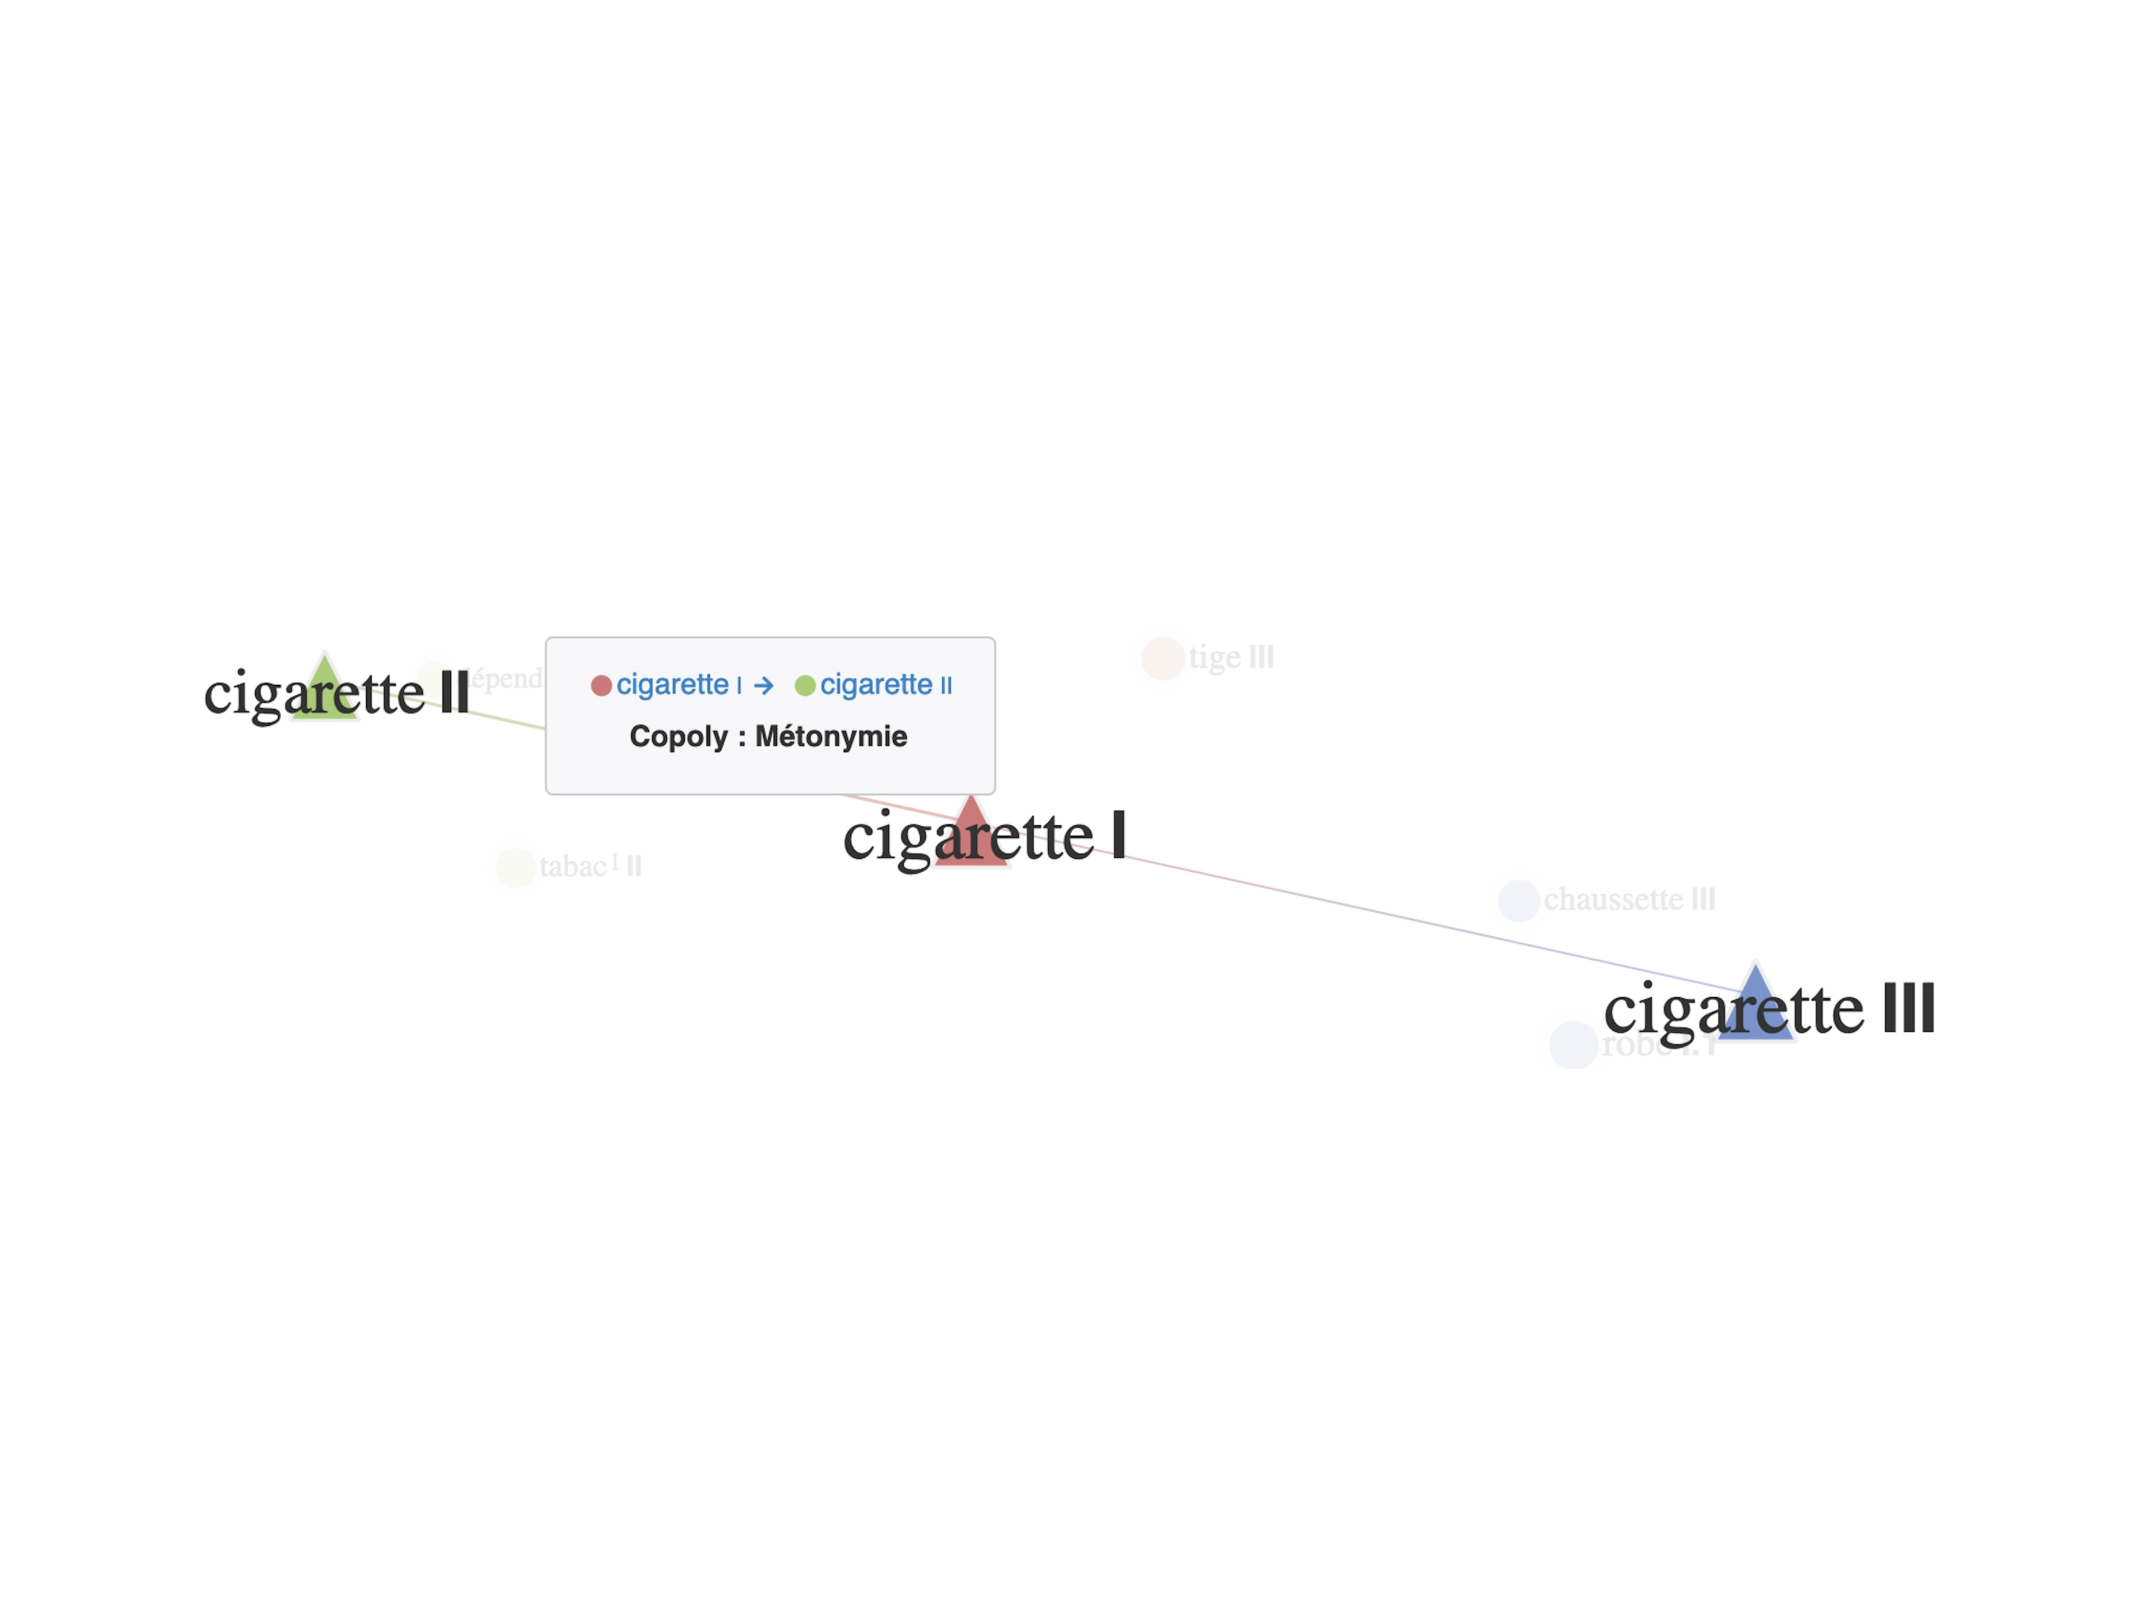
\epsfig{width=8cm,file=Fig/LexicalNetworks/polysemy-Fr-CIGARETTE.pdf}
\caption{Polysemy of {\smaller French}~\textsc{cigarette} as represented in the fr-LN}\label{fig:polysemyCIGARETTE}
\end{figure}

A polysemous vocable is formally encoded in a Lexical System as a subnetwork consisting of nodes connected by copolysemy arcs, as shown in \figref{fig:polysemyCIGARETTE} where two copolysemy arcs originate from the node \textsc{cigarette}\sensenum{I}. The \notion{basic lexical unit}\index[notion]{basic lexical unit of a vocable}\index[notion]{vocable!basic lexical unit of a \tld} of a given vocable -- i.e., the lexical unit that controls the polysemy structure of this vocable -- corresponds to the unique node in the subnetwork that does not have an incoming copolysemy arc in its relational profile\index[notion]{relational profile}\index[notion]{profile, relational}.

\subsubsubsection{Idiom-component relation}\label{sec:idiomComponentRelation}

In a Lexical System, an \notion{idiom-component relation}\index[notion]{lexical relation!idiom-component \tld|emph}\index[notion]{relation!idiom-component \tld|emph}\index[notion]{idiom!\tld-component relation|emph} encodes the presence of a lexeme in the surface-syntactic structure\index[notion]{idiom!surface-syntactic structure [SSyntS] of an \tld}\index[notion]{structure!surface-syntactic \tld\ [SSyntS]}\index[notion]{surface-syntactic!\tld\ structure [SSyntS]} [SSyntS] of an idiom \parencite{Pause2017b,Pause2017a}. This is illustrated in \figref{fig:idiomComponentRelBRAS_CASSE}, with the SSyntS of the French nominal idiom \idiom{\textsc{bras cassé}} lit.~`arm broken' -- which means approximately `bungler' -- and the corresponding idiom-component relations encoded in the fr-LN.

\begin{figure}

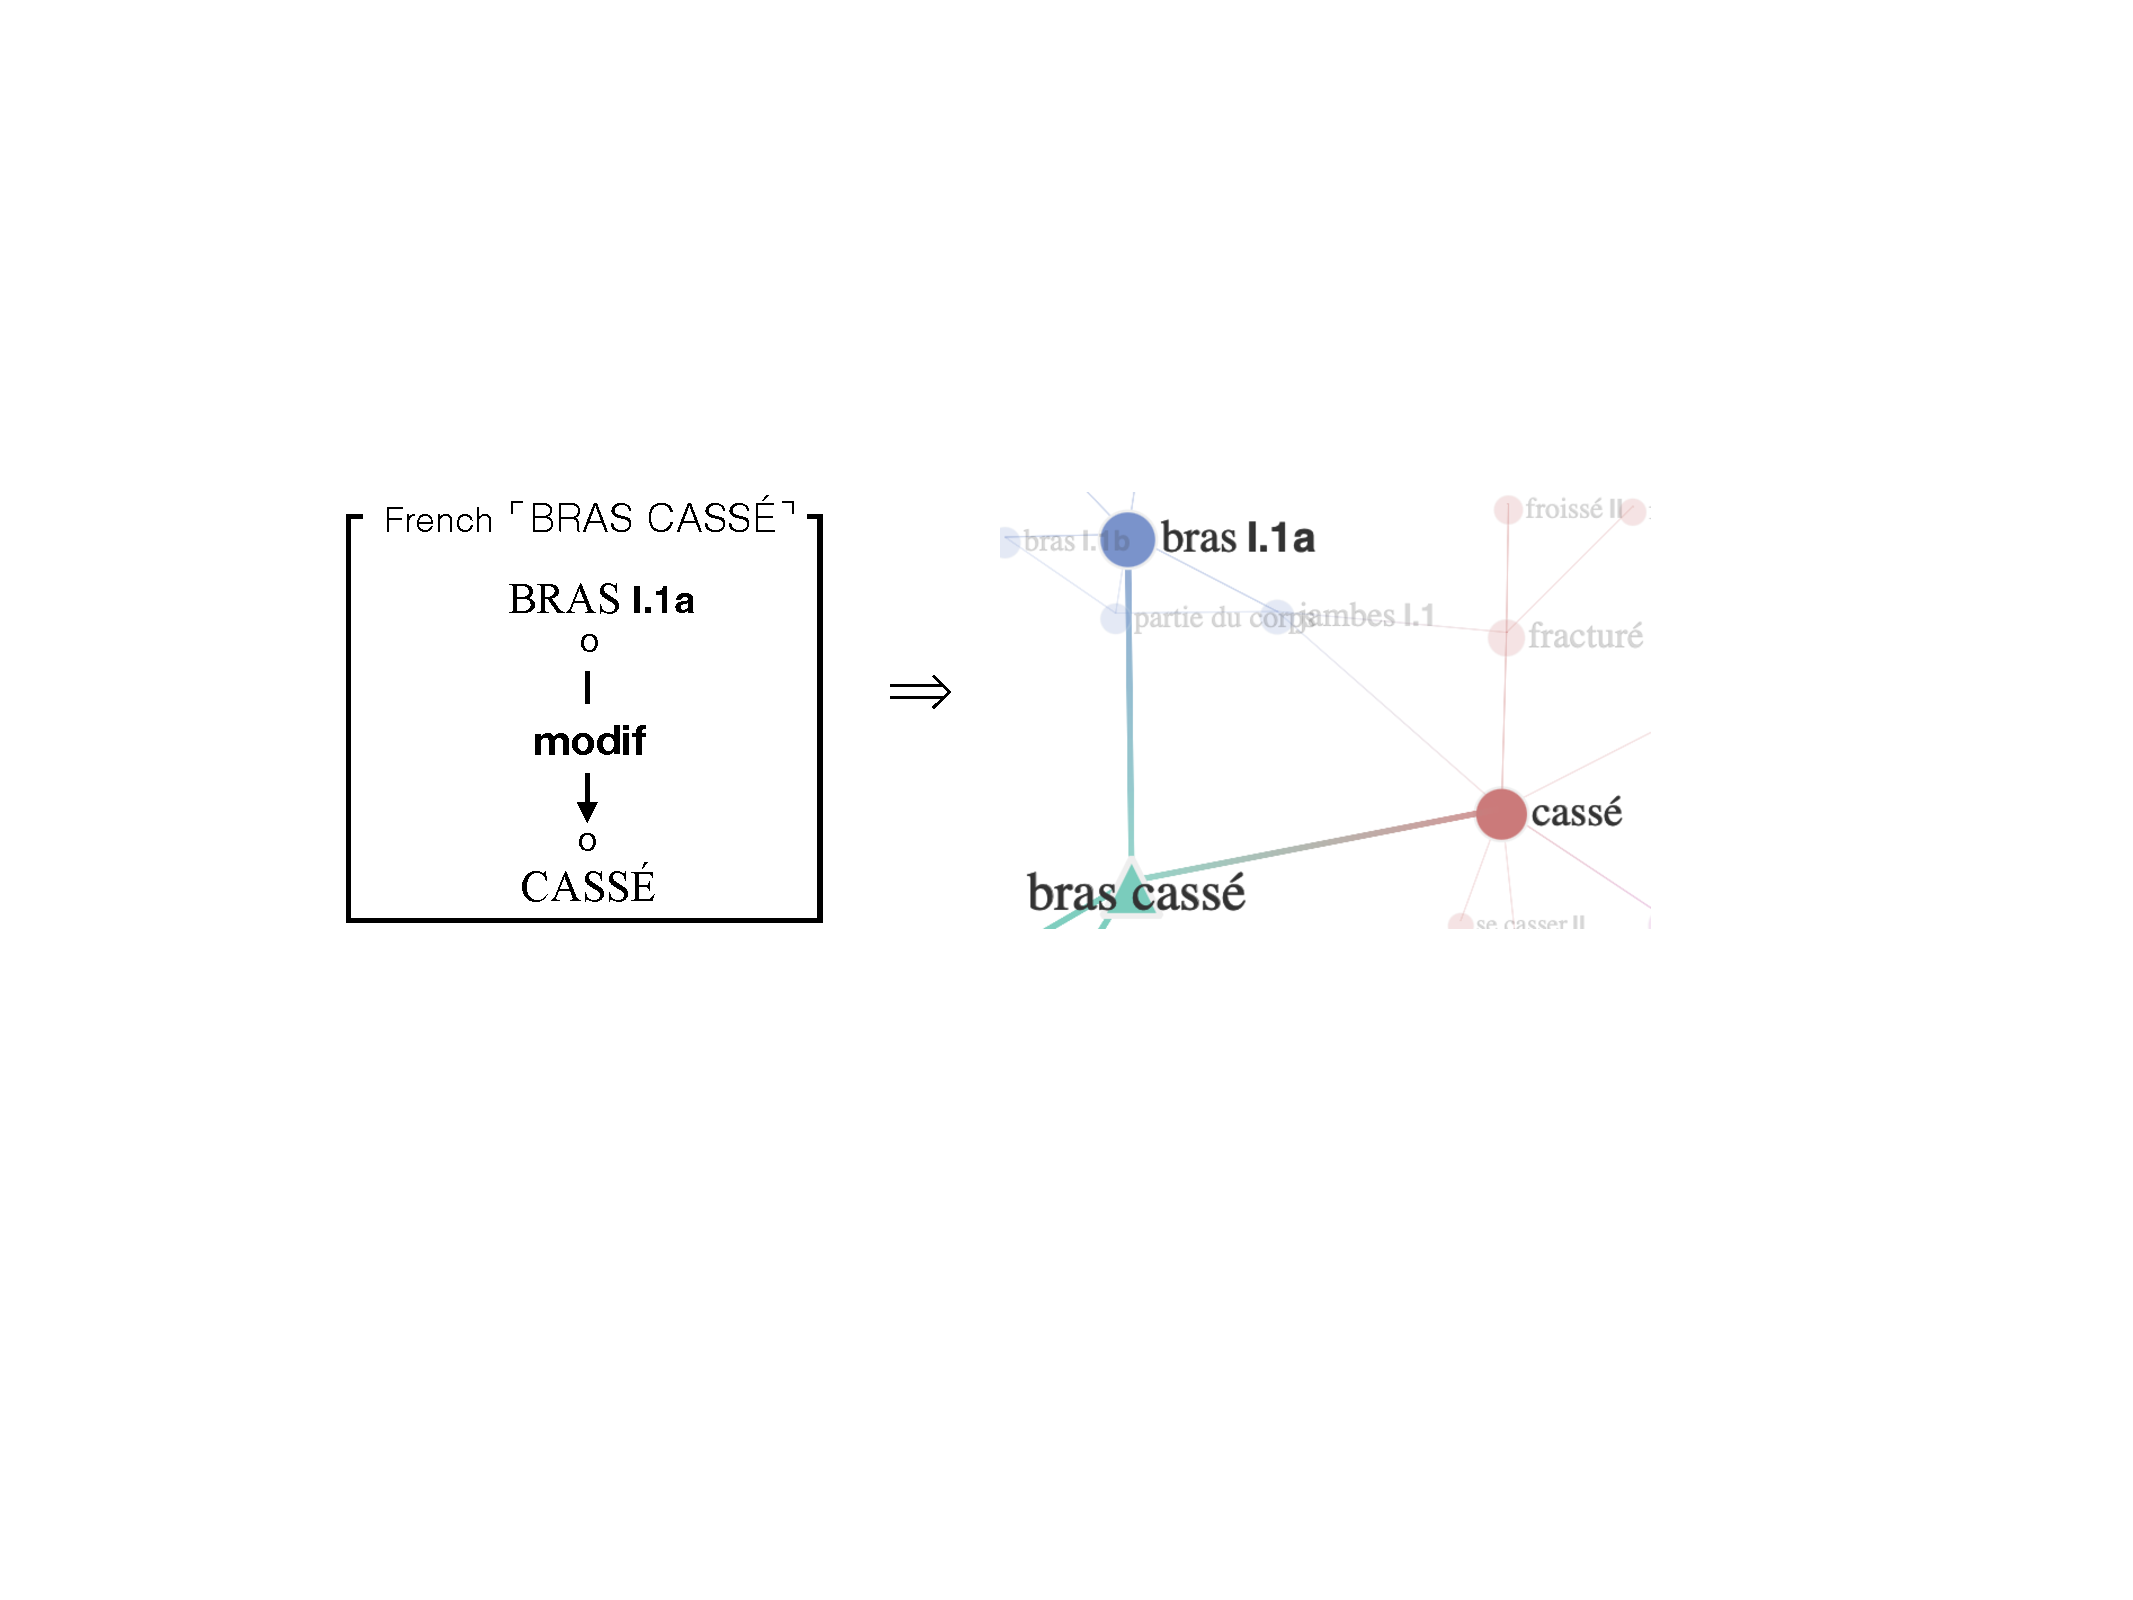
\includegraphics[width=.8\linewidth]{Fig/LexicalNetworks/idiomComponentRelBRAS_CASSE.pdf}
\caption[SSyntS of {\smaller French}~\idiom{\textsc{bras cassé}}~`bungler' and corresponding idiom-component relations in the fr-LN]{SSyntS of {\smaller French}~\idiom{\textsc{bras cassé}} `bungler' together with the two corresponding idiom-component relations encoded in the \mbox{fr-LN}\footnotemark}\label{fig:idiomComponentRelBRAS_CASSE}
\end{figure}\footnotetext{For now, the SSyntS of an idiom is not encoded as such in the fr-LN. Each idiom is associated with a structural pattern that is simply a string of parts of speech slots -- e.g., \texttt{N\thinspace+\thinspace{}Adj}, for \idiom{\textsc{bras cassé}}. These slots are filled with actual lexical units in the description of each individual idiom by encoding idiom-component relations -- for details, see \textcite{Pause2017b}.}

Idiom-component relations belong to the outgoing relational profile\index[notion]{relational profile}\index[notion]{profile, relational} of idioms and, conversely, to the incoming relational profile of the lexemes that compose the idiom. The list of all idioms in which a given lexeme participates is thus directly available in the network structure of a Lexical System and can be shown in the lexical entry of this lexeme, as it is the common practice in Explanatory Combinatorial Dictionaries\index[notion]{Explanatory Combinatorial!\tld\ Dictionary}\index[notion]{dictionary!Explanatory Combinatorial \tld}; see the mention of the idiom \idiom{\textsc{anger management}} at the end of the lexical entry for \textsc{anger}\tsub{(N)} (Appendix, p.\thinspace\pageref{sec:AppendixIdiom}).\footnote{In the lexicography of Lexical Systems, however, this information is encoded while building the description of the idiom, whereas it is usually done while writing the lexical entry of the embedded lexemes in the case of Explanatory Combinatorial Dictionaries and commercial dictionaries as well.}\index[notion]{lexicography!\tld\ of lexical networks}\index[notion]{lexical network!lexicography of \tlds} We give in \tabref{tab:idiomsBRAS} the list of all idioms for which the lexeme \textsc{bras}\sensenum{I.1a} `arm' (cf.~\figref{fig:idiomComponentRelBRAS_CASSE}) is a component in the fr-LN, at the time of writing. This list is automatically extracted from this lexeme's incoming relational profile\index[notion]{relational profile!incoming \tld}\index[notion]{profile, relational!incoming \tld} and displayed in textual visualizations\index[notion]{visualization!textual \tld} of its lexical entry\index[notion]{lexical entry!automatically generated \tld}.

\begin{table}

\footnotesize
\renewcommand*{\arraystretch}{1}
\setlength{\tabcolsep}{2pt}
\begin{tabular}[t]{ l l }
\lsptoprule
\idiom{\textsc{à bras-le-corps}}\sensenum{I}\hspace{5pt}{\relsize{-1.5}lit. `with arm-the-body'} & {\relsize{-1.5}`with both arms around someone's body'} \\
\idiom{\textsc{baisser les bras}}\hspace{5pt}{\relsize{-1.5}lit. `lower the arms'}  & {\relsize{-1.5}`give up'} \\
\idiom{\textsc{bras cassé}}\hspace{5pt}{\relsize{-1.5}lit. `broken arm'} & {\relsize{-1.5}`bungler'} \\
\idiom{\textsc{bras de fer}}\sensenum{I}\hspace{5pt}{\relsize{-1.5}lit. `arm of iron'} & {\relsize{-1.5} `arm-wrestling'} \\
\idiom{\textsc{bras de Morphée}}\hspace{5pt}{\relsize{-1.5}lit. `arms of Morpheus'} & {\relsize{-1.5} `state of sleeping\slashs{}dreaming'} \\
\idiom{\textsc{bras droit}}\hspace{5pt}{\relsize{-1.5}lit. `right arm'} & {\relsize{-1.5} `right-hand person'} \\
\idiom{\textsc{bras long}}\hspace{5pt}{\relsize{-1.5}lit. `long arm'} & {\relsize{-1.5} `the long arm'} \\
\idiom{\textsc{couper bras et jambes}} \lfgp{\textit{à} N\tsub{Y}}\hspace{5pt}{\relsize{-1.5}lit. `cut.off arms and legs [to Y]'} & {\relsize{-1.5} `take the steam out [of person Y]'} \\
\idiom{\textsc{Les bras en tombent}} \lfgp{\textit{à} N\tsub{X}}\hspace{5pt}{\relsize{-1.5}lit. `The arms because.of.this fall [to X]'} & {\relsize{-1.5} `X is completely flabbergasted'}\\
\lspbottomrule
\end{tabular}\caption{Idioms with \textsc{bras}\sensenum{I.1a} `arm' as component in the fr-LN}\label{tab:idiomsBRAS}
\end{table}

An idiom-component relation is \emph{inherently} not a meaning relation\index[notion]{meaning!\tld\ relation}\index[notion]{relation!meaning \tld}: it has a null semantic weight\index[notion]{semantic!\tld\ weight}\index[notion]{weight, semantic}. However, it is not necessarily devoid of \emph{semantic relevance}: it can participate in establishing a semantically relevant path between two lexical nodes of the lexical network.\footnote{On the important notion of path in a graph\slashs{}network, see \sectref{sec:basicsGraphTheory}, p.\thinspace\pageref{txt:pathInAGraph}.}\index[notion]{path in a graph\slashs{}network}\index[notion]{graph!path in a \tld}

Such is the case, obviously, for weak idioms\index[notion]{idiom!weak \tld} (e.g., \idiom{\textsc{frying pan}}), whose definition contains the semantemes of all their lexical components: here, idiom-component relations are somehow doubling meaning-inclusion relations (cf. \sectref{sec:meaningInclusionRelation} below). More unexpectedly, strong idioms\index[notion]{idiom!strong \tld} (e.g., $\ulcorner$\textsc{push} \lfgp{someone's} \textsc{buttons}$\urcorner$) can participate in establishing semantically relevant paths in a lexical network, especially when they are based on metaphors that are transparent and alive in the current state of the language \parencite{Alm-Arvius2006}. To illustrate this, let us consider the idiom \idiom{\textsc{as~snow}}, that functions as \lf{Magn}\index[lf]{Magn@\lf{Magn}} collocate for adjectives such as \textsc{cold}\tsub{(Adj)}, \textsc{pure} or \textsc{white}\tsub{(Adj)}. One of the two idiom-component relations this idiom controls is part of a two-step path connecting the adjective \textsc{white}\tsub{(Adj)} and the noun \textsc{snow}\tsub{(N)}, where each step of the path has a null semantic weight due to the nature of the lexical relation it encodes, as shown in 	\tabref{tab:two-stepPathWHITE-adjSNOW-n}. This unsemantic two-step path is doubling in the lexical network a direct meaning-inclusion relation: \textsc{white}\tsub{(Adj)} is semantically included in \textsc{snow}\tsub{(N)}.\footnote{See `white flakes' in the definition of \textsc{snow}\tsub{(N)} in \chapref{chap:paraLFs}, \sectref{sec:LFapparenteesSynAnti}, p.\thinspace\pageref{ldef:defSNOW-n}.}\index[notion]{definition!lexicographic \tld}

\begin{table}

\footnotesize
\renewcommand*{\arraystretch}{1.2}
\setlength{\tabcolsep}{1pt}
\begin{tabular}{ c >{\raggedright\arraybackslash}p{5.2cm}  >{\raggedright\arraybackslash}p{6.2cm} }
\lsptoprule

\textsf{Steps} & \multicolumn{1}{c}{\textsf{Relations}} & \multicolumn{1}{c}{\textsf{Comments}} \\

\midrule

{\footnotesize 1.} & \textsc{white}\tsub{(Adj)}\thinspace\lexRel{\lf{Magn}}\thinspace\idiom{\textsc{as snow}} & LF relation -- i.e., \lfappl{Magn}{\textit{white}\tsub{(Adj)}}~=~\idiom{\textit{as snow}} \\

{\footnotesize 2.} & \idiom{\textsc{as snow}}\thinspace\lexRel{idiom-comp.}\thinspace\textsc{snow}\tsub{(N)} & \textsc{snow}\tsub{(N)} participates in the SSyntS of the idiom \idiom{\textsc{as~snow}} \\

\lspbottomrule
%\multicolumn{3}{p{12.5cm}}{\vspace{1pt}....} \\
\end{tabular}\caption[Two-step path from \textsc{white}\tsub{(Adj)} to \textsc{snow}\tsub{(N)} based on inherently non-meaning relations]{Two-step path from \textsc{white}\tsub{(Adj)} to \textsc{snow}\tsub{(N)} based on inherently non-meaning relations\footnotemark}\label{tab:two-stepPathWHITE-adjSNOW-n}\index[notion]{idiom!surface-syntactic structure [SSyntS] of an \tld}\index[notion]{structure!surface-syntactic \tld\ [SSyntS]}\index[notion]{surface-syntactic!\tld\ structure [SSyntS]}
\end{table}\footnotetext{Remember that \lfappl{Magn}{L} = L′ entails an inherently non-meaning relation between L and L′ -- \sectref{sec:LFRelationsBackboneOfLFs}, p.\thinspace\pageref{par:semanticWeightLFRelation}.}

The explicit encoding of the above network path within a lexicon model helps account for the great proximity\index[notion]{proximity, lexical} that exists in English between the semantic field of `snow' and the semantic field of `whiteness \lfgp{things that are white}'. This proximity is not a purely conceptual fact: it is linguistically determined. It results from existence in the English language of lexemes and phrasemes -- such as the idiom \idiom{\textsc{as~snow}} -- that are based on the inclusion of the semanteme `white' in the definition of \textsc{snow}\tsub{(N)}.

The above analysis illustrates the important role that idiom-component relations can play in the structuring of the Mental Lexicon\index[notion]{Mental Lexicon}\index[notion]{lexicon!Mental Lexicon}. By encoding these relations in Lexical Systems, we account better for the multiplicity of ways the Speaker\index[notion]{Speaker, the} can navigate from one lexical unit to another during the activation of lexical knowledge; we also account for associations of ideas that take place in the Speaker's mind and can influence lexical selection\index[notion]{lexical access\slashs{}selection}.

\subsubsubsection{Meaning-inclusion relation}\label{sec:meaningInclusionRelation}

A lexicographic definition\index[notion]{definition!lexicographic \tld} is a paraphrase of the defined lexical unit in terms of semantically simpler lexical units\index[notion]{lexical unit!simpler \tld} \parencite{MelcukPolguere2018}.\footnote{Lexical unit L′ is semantically simpler than lexical unit L if and only if L′ appears in the decomposition of the meaning of L, but not vice versa.} Consequently, each defining element in the definition of \textsc{anger}\tsub{(N)} given in \ref{ex:ChapLNDefANGER-n} -- see also the Appendix (p.\thinspace\pageref{def:ANGER-n}) -- is a semanteme\index[notion]{semanteme} corresponding to a specific lexical unit of English.

\begingroup
\small

\ex. \label{ex:ChapLNDefANGER-n}\APolbox{\linewidth}{%
%\renewcommand*{\arraystretch}{1.2}
\setlength{\tabcolsep}{2pt}
\begin{tabular}{ >{\raggedright\arraybackslash}p{3cm} >{\raggedright\arraybackslash}p{7.7cm} }
\textit{X's anger at Y for Z} :
& X's unpleasant, unfavorable feeling directed at person Y and caused by Z -- such that \\
& \textbf{\textsf{Stimulus}} \\
& \setlength{\tabcolsep}{.5pt}\begin{tabular}{ p{0.35cm} >{\raggedright\arraybackslash}p{7cm} }
\SpecDiffIndent & X believes that Y is responsible for Z \\
\SpecDiffIndent & Z is undesirable for X \\
  \end{tabular} \\
& \textbf{\textsf{Effect}} \\
& \setlength{\tabcolsep}{.5pt}\begin{tabular}{ p{0.35cm} >{\raggedright\arraybackslash}p{7cm} }
\SpecDiffIndent & X wants to do something hostile to Y \weakcomp{in order to stop Z} \\
\SpecDiffIndent & X enters in a mental state such that X can easily lose self-control \\
  \end{tabular} \\
%\multicolumn{3}{p{12.5cm}}{\vspace{1pt}....} \\
\end{tabular}
}

\endgroup

From a lexical network viewpoint, this inclusion of lexical units (more precisely, the corresponding semantemes) in the definition translates into a set of \notion{meaning-inclusion relations}\index[notion]{lexical relation!meaning-inclusion \tld|emph}\index[notion]{relation!meaning-inclusion \tld|emph}\index[notion]{meaning!\tld\ inclusion relation|emph} originating from \textsc{anger}\tsub{(N)} and leading to included lexical units.

Meaning-inclusion relations induced by lexicographic definitions are not all equally relevant as regards semantic weight\index[notion]{semantic!\tld\ weight}\index[notion]{weight, semantic}. For instance, the three relations in \Next, induced by the definition of \textsc{anger}\tsub{(N)}, are listed by order of decreasing semantic weight.

\begingroup
\small

\ex. \setlength{\tabcolsep}{2pt}\begin{tabular}{ l l }
\textsc{anger}\tsub{(N)}\thinspace\lexRel{meaning inclusion}\thinspace\textsc{feeling}\tsub{(N)} & -- strong semantic weight \\*
\textsc{anger}\tsub{(N)}\thinspace\lexRel{meaning inclusion}\thinspace\textsc{hostile}\tsub{(Adj)} & -- average semantic weight \\*
\textsc{anger}\tsub{(N)}\thinspace\lexRel{meaning inclusion}\thinspace\textsc{responsible} & -- weak semantic weight \\
\end{tabular}

\endgroup

In many instances, meaning-inclusion relations establish lexical connections that play a significant role in the lexicon and cannot be accounted for by LFs. An LF relation L\thinspace\lexRel{\lf{f}}\thinspace{}L′ (i.e., \lfappl{f}{L}~=~L′) is, first of all, a \emph{combinatorial} relation, that may or may not also be semantic: the meaning \sigmaF\ of \lf{f} is expressed in combination with L by the lexical entity L′. By contrast, an L\thinspace\lexRel{meaning inclusion}\thinspace{}L′ relation is necessarily a purely meaning relation\index[notion]{meaning!\tld\ relation}\index[notion]{relation!meaning \tld}: the fact that the semanteme `L′' is included in the semanteme `L'.

\subsection{Formal properties of Lexical Systems}\label{sec:formalPropertiesLS}

Lexical Systems have a formal structure known in graph theory\index[notion]{graph!\tld\ theory} as a small-world network\index[notion]{network \lfgp{see also \textit{graph}}!small-world \tld}\index[notion]{small-world!\tld\ network}. This characteristic has strong implications for Lexical Systems' computability, so that it is essential to give some consideration to this topic. To present formal properties of Lexical Systems, we start with the introduction of some basic notions of graph theory, the knowledge of which is presupposed for the construction and study of lexical networks\index[notion]{lexical network} (\sectref{sec:basicsGraphTheory}). Next, we use these notions to explain how the informational proximity between lexical units in the Mental Lexicon can be modeled by exploiting the small-world structure of Lexical Systems (\sectref{sec:lexicalProximityTopologicalProximity}). We apologize in advance both:

\begin{itemize}
\item to readers who are unfamiliar with mathematical notions as they may find what follows too technical,
\item to readers with background in graph theory for the simplifications and approximations we operate.
\end{itemize}

\subsubsection{Some basics of graph theory}\label{sec:basicsGraphTheory}

\subsubsubsection{Networks and their mathematical counterparts: graphs}

Until now, we have used the term \notion{network}\index[notion]{network \lfgp{see also \textit{graph}}|emph} in a rather broad sense, which can be glossed as `system of individual entities connected by one-to-one relations'.

Actual networks can be \emph{artificial} (designed) systems: they have been devised as such, to serve specific purposes -- for instance, a city metro system, where metro stations are individual entities and tracks\slashs{}tunnels connecting stations are relations between these entities.

Networks can also be \emph{natural} systems: they happen to exist without having been consciously designed; we are specially interested here in networks constituted of a huge number of entities -- for instance, the system formed in the brain by neurons and their synaptic connections. These very large networks that are natural systems found in our surrounding or remote environment are called \notion{real-world networks}\index[notion]{real-world network\slashs{}graph|emph}\index[notion]{network \lfgp{see also \textit{graph}}!real-world \tld|emph}. Note that, in our use of the term, a real-world network can be the product of human activity -- for instance, the network formed by hyperlinked webpages of the Internet. What matters is that this structure has emerged naturally, unlike the structure of a city metro system, which is relatively small and has been consciously designed.

\phantomsection\label{txt:LSRealWorldNetwork}\begin{soundboxnotitle}
Following Postulate~1 (p.\thinspace\pageref{txt:postulateStrucLexicons}), Mental Lexicons\index[notion]{Mental Lexicon}\index[notion]{lexicon!Mental Lexicon} are natural real-world networks and, following Postulate~2 (p.\thinspace\pageref{txt:postulateStrucLS}), Lexical Systems\index[notion]{Lexical System} are \emph{human-made} networks whose structure is expected to be analogous to the \emph{natural} structure of Mental Lexicons. Therefore, Lexical Systems are considered here as real-world networks as well.
\end{soundboxnotitle}

Networks are studied as formal objects by \notion{graph theory}\index[notion]{graph!\tld\ theory|emph}, a branch of mathematics customarily traced back to \textcite{Euler1741}: it deals with the formal representation and calculus of network systems. Let us provide some terminological clarification:

\begin{itemize}

\item we use the term \notion{graph}\index[notion]{graph|emph} to designate a mathematical object that underlies a network stripped of all (or most of) the attributes of its nodes and arcs;

\item for the sake of simplicity, our presentation of graphs and their properties uses the terms \textit{node}\index[notion]{node of a network\slashs{}graph} and \textit{arc}\index[notion]{arc of a network\slashs{}graph}, more habitual in linguistic works, even though two other terms are generally favored in graph theory literature, respectively: \textit{vertex} (pl.~\textit{vertices})\index[notion]{vertex \lfgp{pl.~\textit{vertices}}|see{node of a network\slashs{}graph}} and \textit{edge}\index[notion]{edge|see{arc of a network\slashs{}graph}}. 

\end{itemize}

\subsubsubsection{Graph representations}

Graphs are mathematical -- therefore, informational -- objects. They should not be equated with \notion{graph representations}\index[notion]{graph!\tld\ representation}, which are used throughout the present chapter. \figref{fig:undirectedGrapRep} gives three common modes of representation for a given \notion{undirected graph}\index[notion]{graph!undirected \tld} $\mathcal{G}$, i.e., a graph whose arcs are not oriented: geometric representation, set-theoretic representation and adjacency matrix.

\begin{figure}

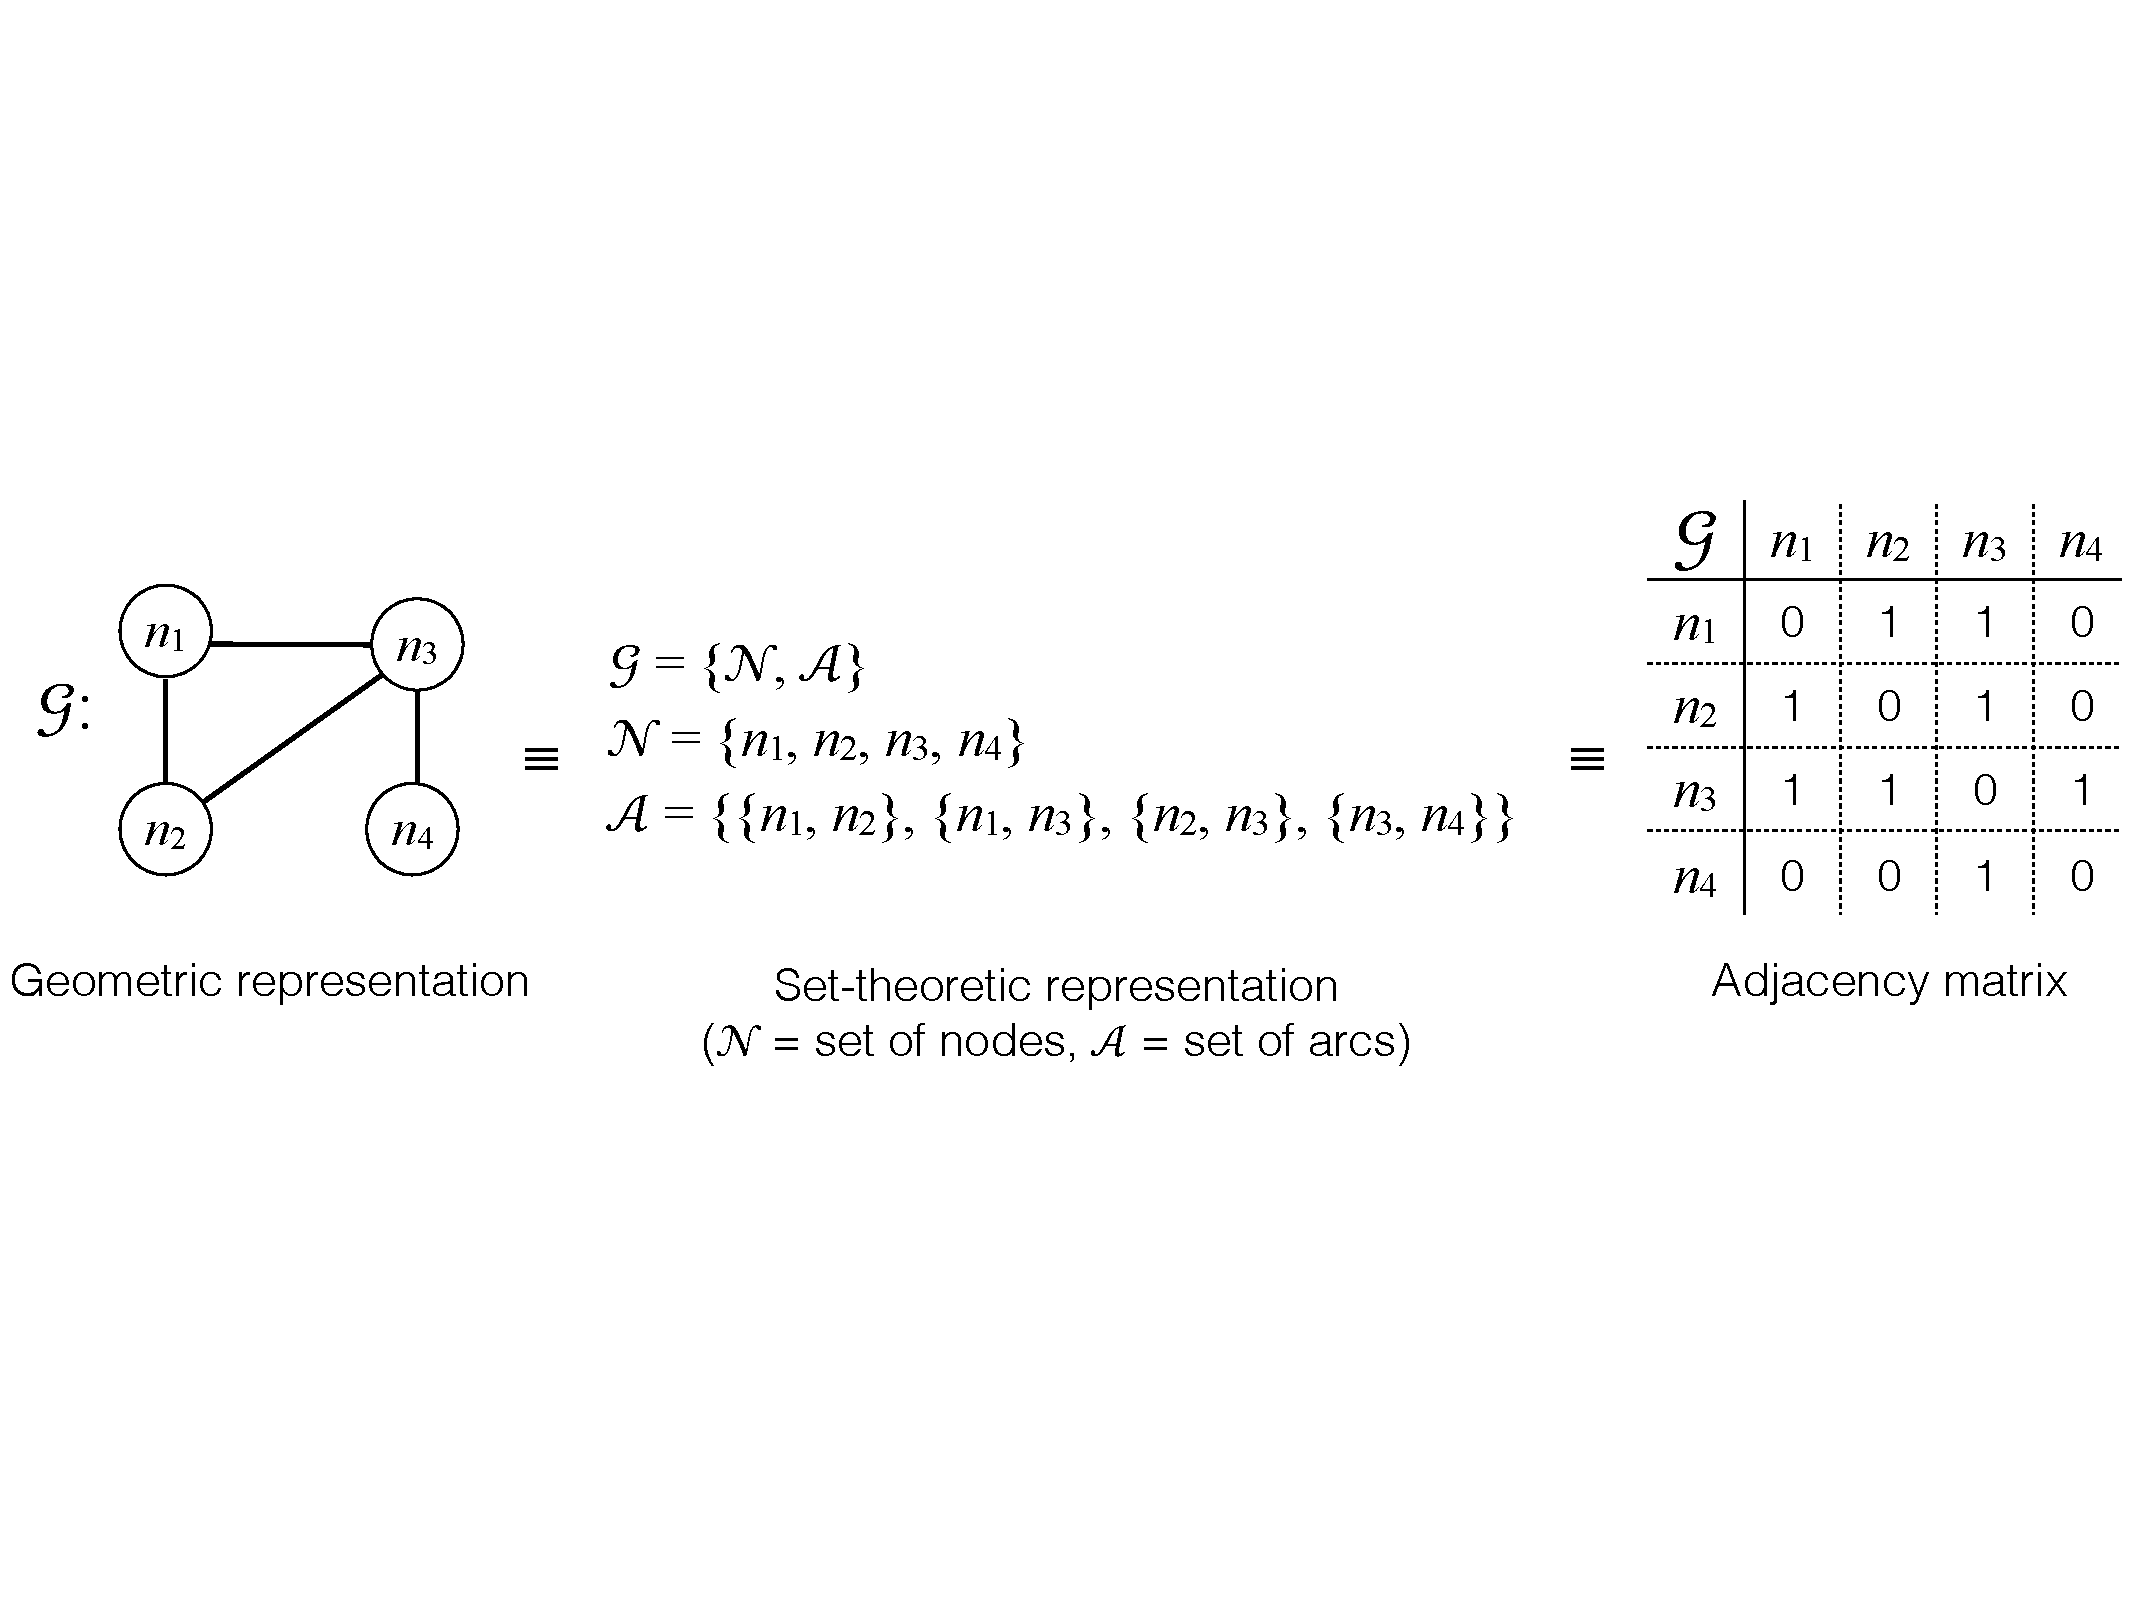
\includegraphics[width=\linewidth]{Fig/LexicalNetworks/undirectedGrapRep.pdf}
\caption{Three modes of representing a given undirected graph $\mathcal{G}$}\label{fig:undirectedGrapRep}
\end{figure}

The \notion{geometric representation}\index[notion]{graph!geometric representation of a \tld} is almost self-explanatory. In our figure, we put node names inside the circles representing nodes in order to highlight the fact that such names are only node IDs, and not attributes of the nodes.\footnote{This is in reference to what was said earlier about the distinction we maintain between the terms \textit{network} and \textit{graph} (network stripped of non-structural information).} A graph is entirely defined by its \notion{topology}\index[notion]{topology|emph}\index[notion]{graph!topology of a \tld|emph}\phantomsection\label{txt:topology}: its system of nodes and connecting arcs. Consequently, in a graph geometric representation, the spacial distribution\index[notion]{node of a network\slashs{}graph!geometric distribution of \tlds}\index[notion]{geometric distribution of graph nodes} of nodes and arcs is irrelevant from a formal point of view and only serves legibility purposes.\footnote{We will show (\sectref{sec:lexicalProximityTopologicalProximity}, p.\thinspace\pageref{sec:lexicalProximityTopologicalProximity}) that geometric distribution of nodes can nonetheless be used to encode additional information about the graph's overall topology.} The relative positioning of nodes in the geometric representation of \figref{fig:undirectedGrapRep} can be totally upended (\textit{n}\tsub{4} at the very top, \textit{n}\tsub{1} below \textit{n}\tsub{3}, \textit{n}\tsub{2} positioned much closer to \textit{n}\tsub{3}, etc.); it will remain the representation of the same graph $\mathcal{G}$ as long as connections established by the arcs remain identical.

The \notion{set-theoretic representation}\index[notion]{graph!set-theoretic representation of a \tld} defines a graph as a mathematical set comprised of two subsets: (i)~a set of nodes and (ii)~a set of arcs; this latter set contains unordered two-element sets encoding non-oriented binary relations between nodes.

The \notion{adjacency matrix}\index[notion]{adjacency matrix (of a graph)}\index[notion]{graph!adjacency matrix of a \tld} is a table where each row and each column correspond to a node of the graph; each cell of the table indicates whether an arc connects the corresponding nodes: \textsf{1} means that the nodes are connected and \textsf{0} means that they are not. The adjacency matrix for graph $\mathcal{G}$ (\figref{fig:undirectedGrapRep}) is symmetrical\index[notion]{adjacency matrix (of a graph)!(non-)symmetrical \tld} relative to the table's top-left to bottom-right diagonal; this comes from the fact that, the arcs being non-oriented, any \textit{n}---\textit{n}′ arc is equally an \textit{n}′---\textit{n} arc.

We exemplified the three modes of representation above with an undirected graph for pedagogical purposes. However, lexical relations examined earlier in \sectref{sec:mainCharacteristicsLS} are all oriented and, therefore, the graphs underlying Lexical Systems\index[notion]{graph!Lexical System \tld}\index[notion]{Lexical System!\tld\ graph} are \notion{directed graphs}\index[notion]{graph!directed \tld}. \figref{fig:directedGrapRep} gives the three representations of a directed graph $\mathcal{G}^\prime$.

\begin{figure}

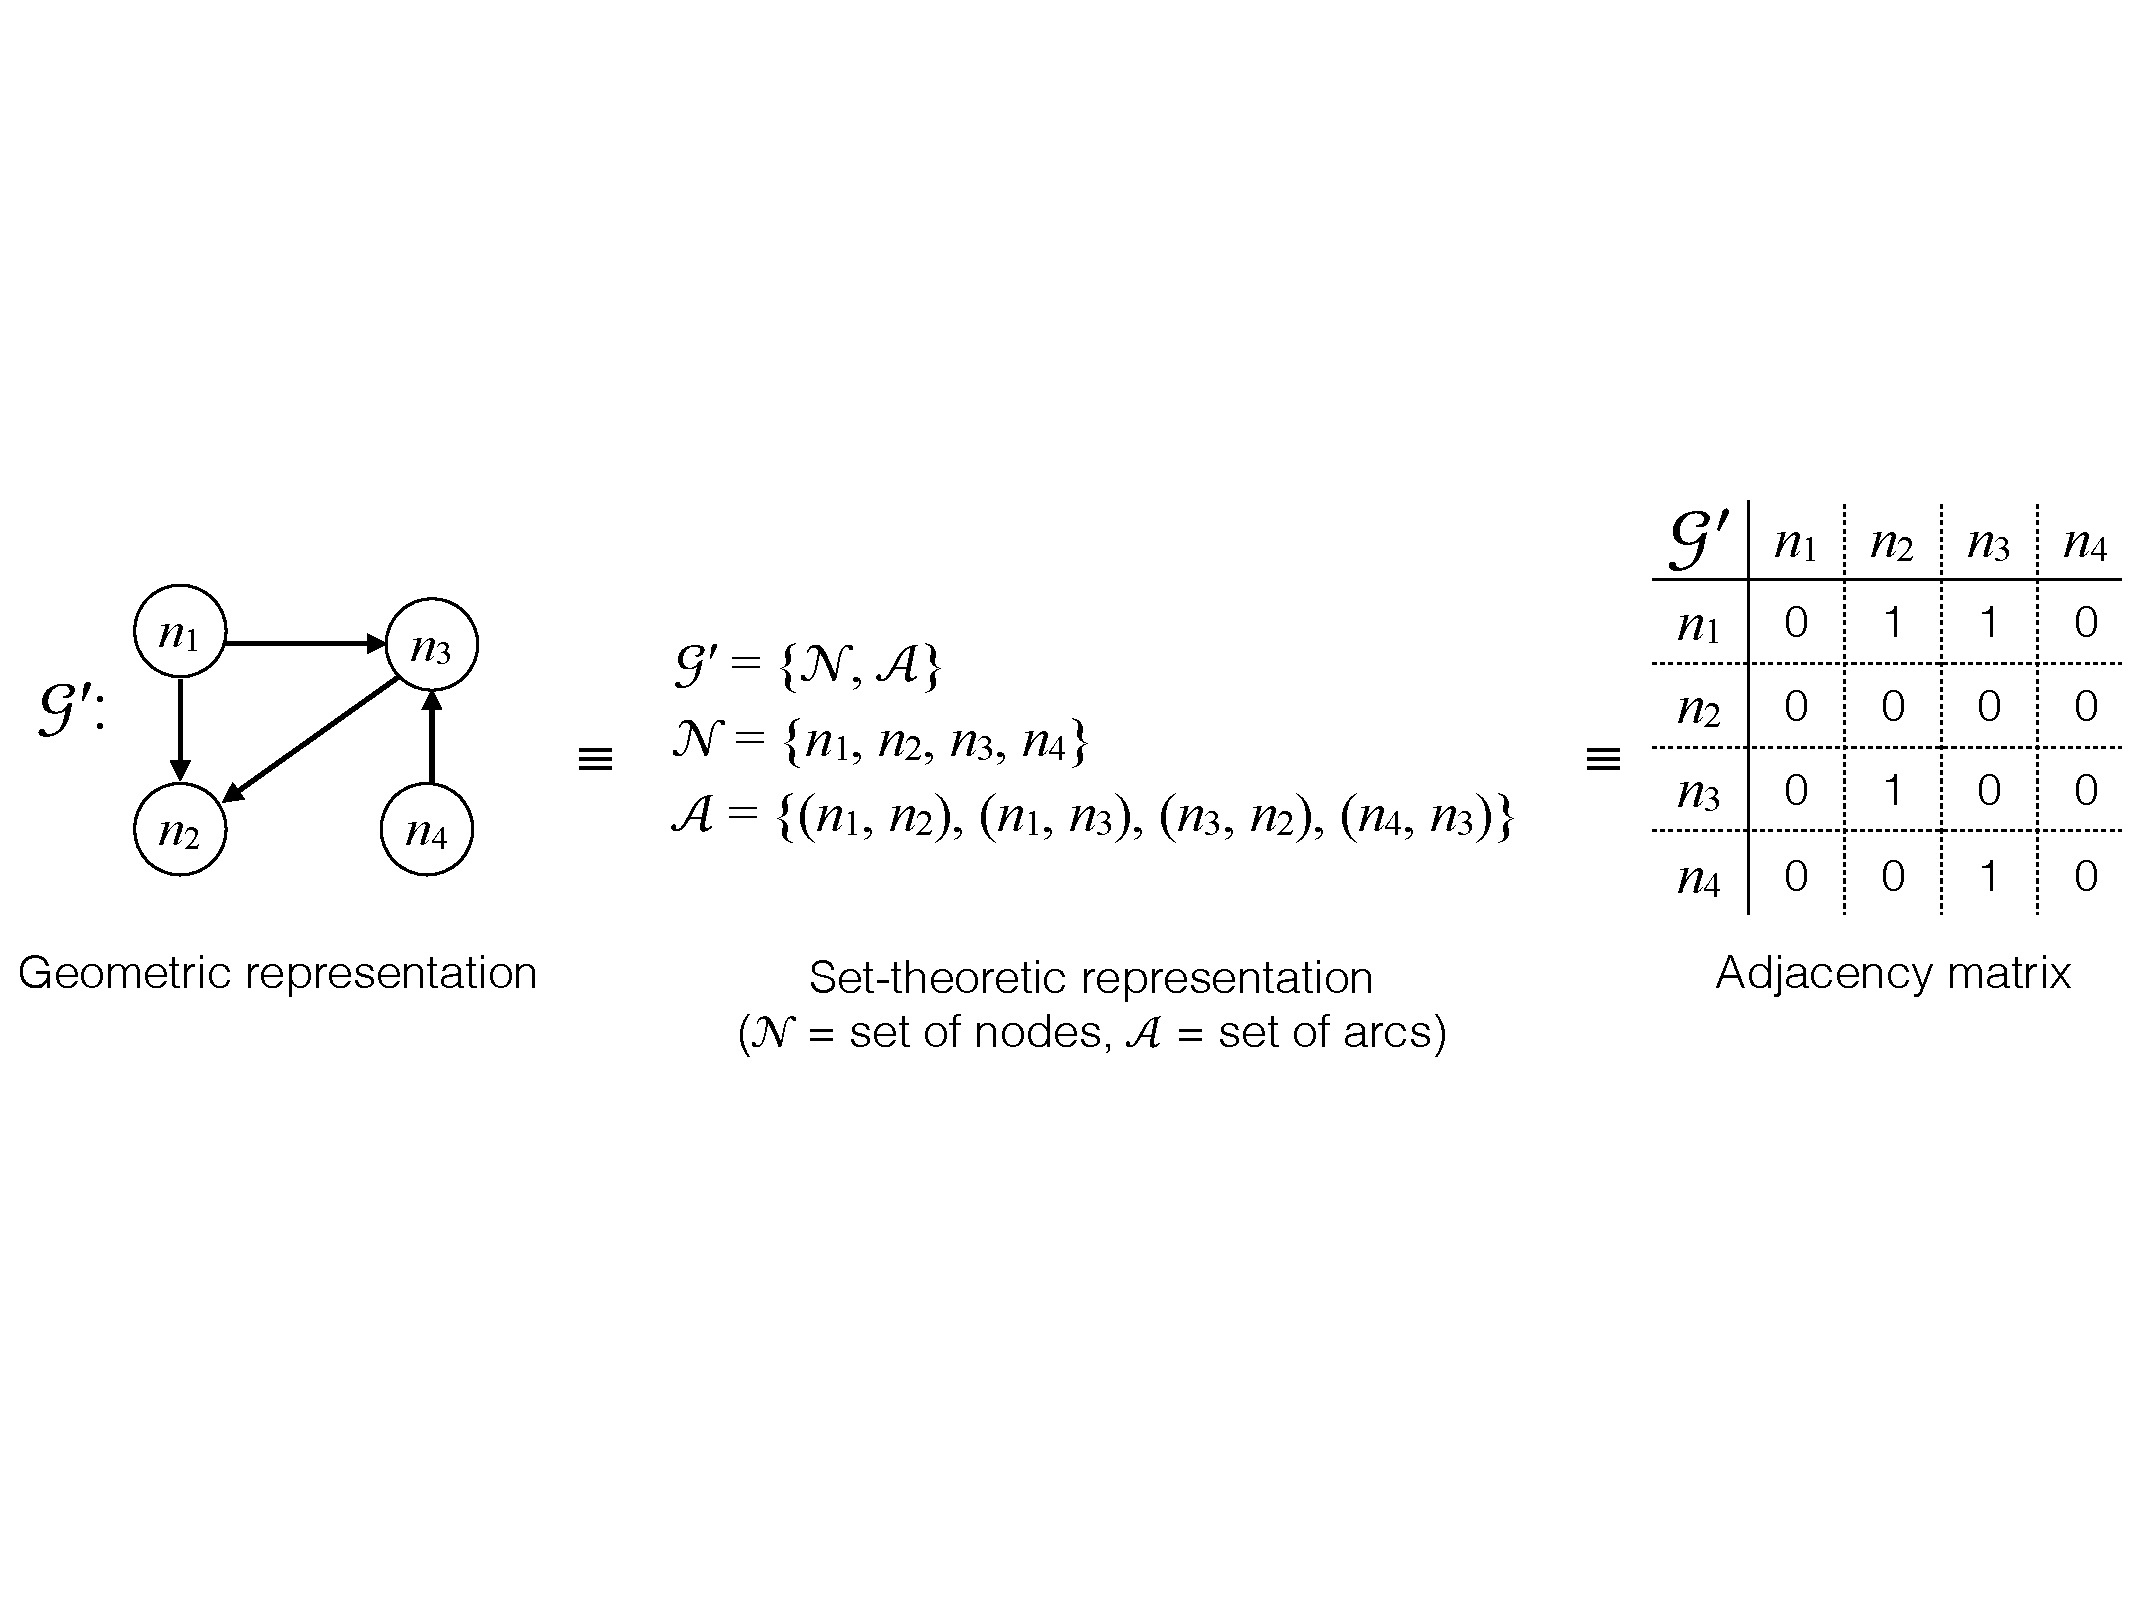
\includegraphics[width=\linewidth]{Fig/LexicalNetworks/directedGrapRep.pdf}
\caption{Three modes of representing a given directed graph $\mathcal{G}^\prime$}\label{fig:directedGrapRep}
\end{figure}

%https://medium.com/basecs/from-theory-to-practice-representing-graphs-cfd782c5be38
Differences with the representations of \figref{fig:undirectedGrapRep} (an undirected graph) are as follows:

\begin{itemize}

\item arcs of the geometric representations are \emph{arrows}\index[notion]{arrow of a network\slashs{}graph [=~arc]}\index[notion]{network \lfgp{see also \textit{graph}}!arrow of a \tld} -- they indicate the \notion{starting node} and the \notion{end node}\index[notion]{node of a network\slashs{}graph!starting\slashs{}end \tld} for each relation;

\item the set of arcs $\mathcal{A}$ in the set-theoretic representation contains (ordered) \mbox{\emph{couples}} of nodes -- instead of (unordered) two-element sets of nodes;

\item \textsf{1}s and \textsf{0}s in the adjacency matrix take into account, for each cell, which node is the starting node and which node is the end node of the corresponding relation; note that the adjacency matrix of graph $\mathcal{G}^\prime$ is non-symmetrical\index[notion]{adjacency matrix (of a graph)!(non-)symmetrical \tld}.

\end{itemize}

One of the advantages of the geometric representation of graphs over the two other representations is that it offers a clear visualization of possible paths between nodes. A \notion{path}\index[notion]{path in a graph\slashs{}network|emph}\index[notion]{graph!path in a \tld|emph}\phantomsection\label{txt:pathInAGraph} in a graph is a sequence of arcs that connects a sequence of nodes where neither arcs nor nodes are repeated. In an oriented graph, one can consider \notion{directed paths}\index[notion]{path in a graph\slashs{}network!directed \tld} -- the sequence of arcs follows the orientation of the arcs -- or \notion{undirected paths}\index[notion]{path in a graph\slashs{}network!undirected \tld} -- the orientation of arcs is not relevant. For instance, the geometric representation of \figref{fig:directedGrapRep} clearly shows:

\begin{itemize}

\item two directed paths from \textit{n}\tsub{1} to \textit{n}\tsub{2}, namely: \textit{n}\tsub{1}-\textit{n}\tsub{2} and \textit{n}\tsub{1}-\textit{n}\tsub{3}-\textit{n}\tsub{2};

\item two undirected paths from \textit{n}\tsub{1} to \textit{n}\tsub{4}, namely: \textit{n}\tsub{1}-\textit{n}\tsub{3}-\textit{n}\tsub{4} and \textit{n}\tsub{1}-\textit{n}\tsub{2}-\textit{n}\tsub{3}-\textit{n}\tsub{4}.

\end{itemize}

The notion of path is central in the definition of small-world networks\index[notion]{network \lfgp{see also \textit{graph}}!small-world \tld}\index[notion]{small-world!\tld\ network} (see \sectref{sec:smallWorldNetworks}, p.\thinspace\pageref{sec:smallWorldNetworks}).

\subsubsubsection{Structural properties of Lexical System graphs}

Graphs are characterized by structural properties\index[notion]{graph!structural property of a \tld} that pertain, primarily, (i)~to the nature of their arcs -- for instance, we have already established that we are concerned here with directed graphs only -- and (ii)~to the types of node-arc configurations they contain. We concentrate on \notion{Lexical System graphs}\index[notion]{graph!Lexical System \tld|emph}\index[notion]{Lexical System!\tld\ graph|emph} -- referred to as $\mathcal{G}_{LS}$ -- and identify four properties (A--D) that characterize them as a specific type of directed graph\index[notion]{graph!directed \tld}. These properties are listed below, then summarized and exemplified in \figref{fig:propertiesOfGLS} (p.\thinspace\pageref{fig:propertiesOfGLS}).

\begin{enumerate}

\item[A)] Labeled graph.\enskip\index[notion]{graph!labeled \tld}Each arc of a $\mathcal{G}_{LS}$ is defined by a starting node, an end node and a \notion{label}\index[notion]{label of a network\slashs{}graph arc} that identifies the lexical relation encoded by the arc: LF relation, copolysemy relation, etc. This characterizes a $\mathcal{G}_{LS}$ as an oriented \notion{labeled graph}.

\item[B)] Weighed graph.\enskip\index[notion]{graph!weighed \tld}When presenting LF and non-LF relations encoded in Lexical Systems, we have indicated that these relations can be distinguished according to their semantic weight\index[notion]{semantic!\tld\ weight}\index[notion]{weight, semantic} (\sectref{sec:LFRelationsBackboneOfLFs}, p.\thinspace\pageref{par:semanticWeightLFRelation}). This information is encoded in a $\mathcal{G}_{LS}$ for each arc of the graph, concurrently with the arc label, which characterizes a $\mathcal{G}_{LS}$ as a \notion{weighed graph}.

\item[C)] Multigraph.\enskip\index[notion]{graph!multi\tld}Two nodes of a $\mathcal{G}_{LS}$ can be connected by more than one arc -- for instance, when two lexical units are connected simultaneously by an LF relation and a meaning-inclusion relation\index[notion]{lexical relation!meaning-inclusion \tld}\index[notion]{relation!meaning-inclusion \tld}\index[notion]{meaning!\tld\ inclusion relation}, as in \Next. This results in \notion{multiple arcs}\index[notion]{arc of a network\slashs{}graph!multiple \tlds} in a $\mathcal{G}_{LS}$, which characterizes it as a \notion{multigraph}.

\begingroup
\small

\ex. \setlength{\tabcolsep}{2pt}
\begin{tabular}[t]{ l l >{\raggedright\arraybackslash}p{7cm} }
\lfappl{Gener}{\textit{gas}\tsub{(N)}} & = & \textit{substance} \\*
\multicolumn{3}{l}{\textsc{gas}\tsub{(N)}\thinspace\lexRel{meaning inclusion}\thinspace\textsc{substance}} \\*
\multicolumn{3}{l}{\lfgp{Where `substance' is the central component in the definition of \textsc{gas}\tsub{(N)}}}
\end{tabular}

\endgroup\index[lf]{Gener@\lf{Gener}}\index[notion]{component of a definition!central \tld}\index[notion]{definition!central component of a \tld}

\item[D)] Cyclic graph.\enskip\index[notion]{graph!cyclic \tld}A $\mathcal{G}_{LS}$ contains \notion{cycles}\index[notion]{cycle in a graph\slashs{}network}\index[notion]{graph!cycle in a \tld}, i.e., directed paths\index[notion]{path in a graph\slashs{}network!directed \tld} that originate and end at the same given node. This characterizes a $\mathcal{G}_{LS}$ as a \notion{cyclic graph}. For instance, the set of LF relations in \Next is encoded as a two-step cycle in the corresponding $\mathcal{G}_{LS}$.

\begingroup
\small

\ex. \setlength{\tabcolsep}{2pt}
\begin{tabular}[t]{ l l >{\raggedright\arraybackslash}p{7cm} }
\lfappl{S\tsub{0}}{\textit{present}\tsub{(V)}} & = & \textit{presentation} \\*
\lfappl{V\tsub{0}}{\textit{presentation}} & = & \textit{present}\tsub{(V)}
\end{tabular}

\endgroup\index[lf]{S0@\lf{S\tsub{0}}}\index[lf]{V0@\lf{V\tsub{0}}}

The cycle in \Last also corresponds to a multigraph configuration -- see property C) above.

\end{enumerate}

The above four properties are recapitulated in \figref{fig:propertiesOfGLS}, with illustrations that apply to several properties wherever it is convenient to do so.

\begin{figure}

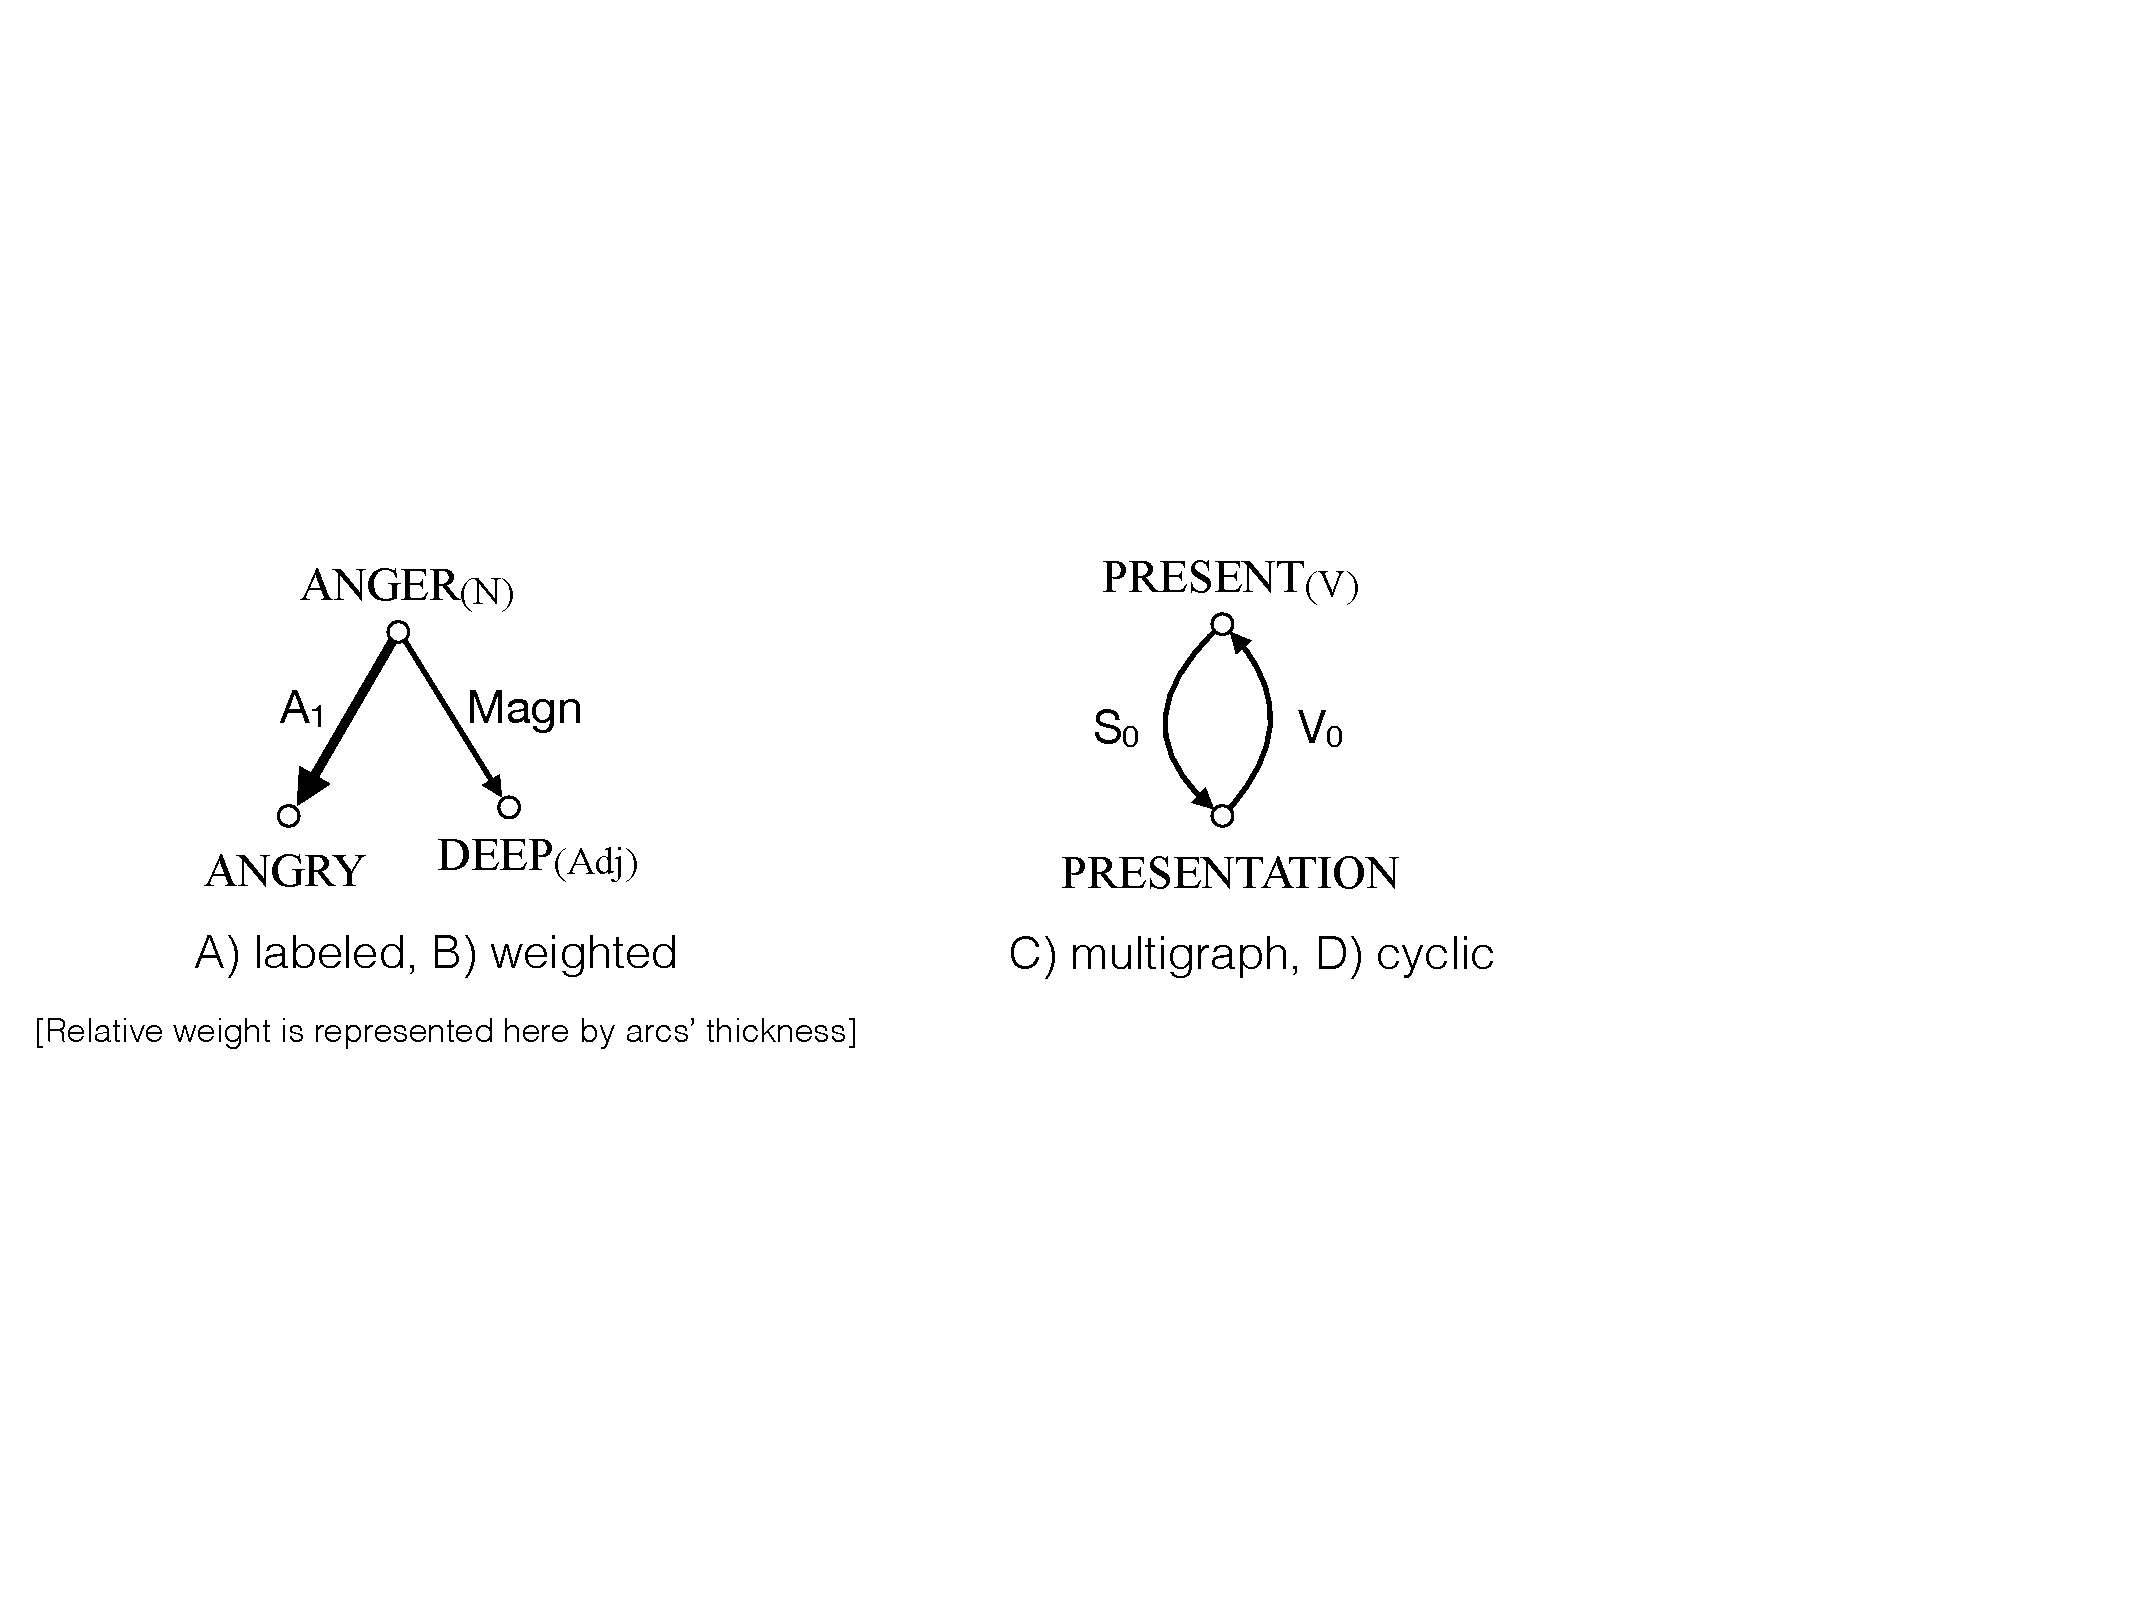
\includegraphics[width=0.8\linewidth]{Fig/LexicalNetworks/propertiesOfGLS.pdf}
\caption{Four structural properties of a Lexical System graph $\mathcal{G}_{LS}$}\label{fig:propertiesOfGLS}
\end{figure}

\subsubsubsection{Lexical Systems as small-world networks}\label{sec:smallWorldNetworks}

The properties examined above characterize a $\mathcal{G}_{LS}$ at a \notion{microscopic} level\index[notion]{microscopic structure (of a graph)}, i.e., at the level of individual nodes and relations they participate in. We are now taking a bird's-eye view of such graphs in order to contrast their microscopic and \notion{macroscopic}\index[notion]{macroscopic structure (of a graph)}\index[notion]{graph!microscopic vs. macroscopic structure of a \tld} structures. For this, we focus on a natural law that tends to apply to all real-world networks\index[notion]{real-world network\slashs{}graph}\index[notion]{network \lfgp{see also \textit{graph}}!real-world \tld} (as characterized in \sectref{sec:basicsGraphTheory}, p.\thinspace\pageref{sec:basicsGraphTheory}).

\begin{soundboxnotitle}
Graph theory\index[notion]{graph!\tld\ theory} has determined that graphs of real-world networks have characteristic topological\index[notion]{topology}\index[notion]{graph!topology of a \tld} properties that identify them as \notion{small-world} \mbox{\textit{networks}}\index[notion]{network \lfgp{see also \textit{graph}}!small-world \tld|emph}\index[notion]{small-world!\tld\ network|emph} \parencite{WattsStrogatz1998}.
\end{soundboxnotitle}

The term \emph{small-world network} refers to the small-world phenomenon\index[notion]{small-world!\tld\ phenomenon} in social networks,\footnote{By \textit{social network}, we mean here social structures made up of individuals having social interactions. We are not referring to social media platforms on the Internet.} which can be presented as follows: there is a high probability for any two randomly selected individuals $i_1$ and $i_2$ to be connected through a relatively short chain of acquaintances \parencite[163]{Kleinberg2000} -- hence the expression \textit{It's a small world!} Though this phenomenon was originally conceptualized from the perspective of social and psychological studies \parencite{Milgram1967}, it is a characteristic feature of real-world networks of any kind. The topological structure of a small-world network has (at least) the four properties (A--D) described below; in order to anchor what follows more directly to our topic of interest (i.e., Lexical Systems), these properties are introduced as properties of a given $\mathcal{G}_{LS}$.\footnote{We try to keep what follows as little mathematical as possible, at the expense of accuracy. See \textcite{GaumeEtAl2010} for a purely mathematical characterization of lexical graphs as small-world networks; see \textcite[Sec.~3]{GaderEtAl2014a-e} for the measurement of the \textit{pedigree} of Lexical Systems as small-world networks.}

\begin{enumerate}

\item[A)] Mainly connected graph.\enskip\index[notion]{graph!(dis)connected \tld}A $\mathcal{G}_{LS}$ may contain some isolated tiny subgraphs (possibly, isolated nodes); however, the bulk of its structure forms one huge \notion{connected graph}: a graph in which there exists at least one path\index[notion]{path in a graph\slashs{}network}\index[notion]{graph!path in a \tld} connecting any two nodes.

\item[B)] Sparse graph.\enskip\index[notion]{graph!sparse \tld}The arc-to-node ratio in a $\mathcal{G}_{LS}$ is low: there are more arcs than nodes, but the difference is not drastic. Consequently, there is an extremely low probability for any two nodes in a $\mathcal{G}_{LS}$ to be \emph{directly} connected. This characterizes a $\mathcal{G}_{LS}$ as a \notion{sparse graph}.\footnote{\label{fn:nodeDegree}The mathematical measurement used to evaluate this sparsity is the \emph{average node degree} of the graph (the average number of arcs connected to each node) -- for lexical networks, see \textcite[Sec.~2]{GaumeEtAl2010}.}

\item[C)] It's a small world, nonetheless!\enskip In spite of its sparsity, a $\mathcal{G}_{LS}$ displays the small-world phenomenon in the sense that any two nodes of $\mathcal{G}_{LS}$, no matter how distant they may be in the topological structure of the graph, are connected by at least one relatively short path. This phenomenon is mainly made possible by two factors.

First, though most nodes of $\mathcal{G}_{LS}$ are weakly connected, there are nodes that function as lexical hubs from a relational viewpoint; for instance:

\begin{itemize}

\item generic terms\index[notion]{generic term} that identify large lexical classes (\textsc{animal}, \textsc{vehicle}, \textsc{feeling}, ...) and thus are ending nodes\index[notion]{node of a network\slashs{}graph!starting\slashs{}end \tld} of many \lf{Gener} arcs\index[lf]{Gener@\lf{Gener}};
\item collocative lexical units\index[notion]{lexical unit!collocative \tld} forming collocations\index[notion]{collocation!base of a \tld} with a large spectrum of potential bases\index[notion]{base!\tld\ of a collocation} -- for instance, the \lf{Magn}\index[lf]{Magn@\lf{Magn}} value \textsc{heavy}\tsub{(Adj)}\sensenum{2} mentioned in \sectref{sec:LFRelationsBackboneOfLFs}, p.\thinspace\pageref{txt:HEAVY-Adj-2}.

\end{itemize}

Second, many copolysemy\index[notion]{polysemy!co\tld}\index[notion]{copolysemy}\index[notion]{lexical relation!copolosemy \tld}\index[notion]{relation!copolysemy \tld} and idiom-component relations\index[notion]{lexical relation!idiom-component \tld}\index[notion]{relation!idiom-component \tld}\index[notion]{idiom!\tld-component relation} in a $\mathcal{G}_{LS}$ establish direct paths between semantic areas that are otherwise very far apart; for instance:

\begin{itemize}

\item \lu{crane}{(N)}{}{I} \lfgp{animals}\thinspace\lexRel{copolysem. metaphor}\thinspace\lu{crane}{(N)}{}{II} \lfgp{machines};

\item \idiom{\textsc{go bananas}} \lfgp{feelings\slashs{}behaviors}\thinspace\lexRel{idiom-comp.}\thinspace\textsc{banana} \lfgp{fruits}.

\end{itemize}

\item[D)] High clustering rate.\enskip\phantomsection\label{par:highClusteringRate}A $\mathcal{G}_{LS}$ is sparse at a macroscopic level\index[notion]{macroscopic structure (of a graph)} but dense at a microscopic level\index[notion]{microscopic structure (of a graph)}\index[notion]{graph!microscopic vs. macroscopic structure of a \tld}, where a profusion of small node clusters\index[notion]{cluster of nodes in a graph}\index[notion]{node of a network\slashs{}graph!cluster of \tlds} are found. In mathematical terms, a $\mathcal{G}_{LS}$ has a high \notion{clustering rate}\index[notion]{cluster of nodes in a graph!clustering rate|emph}\index[notion]{graph!clustering rate of a \tld|emph}: there is a much higher probability for two nodes \textit{n}\tsub{1} and \textit{n}\tsub{2} to be directly connected if both of them are directly connected to a node \textit{n}\tsub{3} than if they are randomly selected. This is easily illustrated with LF relations, where various clustering \notion{inference rules}\index[notion]{inference rule} such as \Next and \NNext can be established. \figref{fig:LFClusters} visualizes linguistic illustrations given in \Next and \NNext.

\begingroup
\small

\ex.\label{ex:clusteringInfRule1} \emph{If} \lfappl{f}{L} = L′\textbf{,} L′′ \\*
         \emph{then} there exists \lfappl{Syn\slashs{}Syn\tsub{$\supset$}\slashs{}Syn\tsub{$\subset$}\slashs{}Syn\tsub{$\cap$}}{L′} = L′′;\footnote{This is true because all the elements of an LF value must be (quasi-)synonymous.} for instance:\\*
\textbullet\hspace{2pt} \lfappl{S\tsub{2}}{\textit{married}} = \textit{spouse}\tsub{(N)}\textbf{,} \idiom{\textit{better half}}\\*
\textbullet\hspace{2pt} \lfappl{Syn\tsub{$\cap$}}{\textit{spouse}\tsub{(N)}} = \idiom{\textit{better half}}

\endgroup\index[lf]{Si@\lf{S\tsub{i}}!\lf{S\tsub{2}}}\index[lf]{Syn@\lf{Syn}!\lf{Syn\tsub{$\cap$}}}

\begingroup
\small

\ex.\label{ex:clusteringInfRule2} \emph{If} \lfappl{f\tsub{1}}{L} = L′ \emph{and} \lfappl{f\tsub{2}}{L′} = L′′ \\*
         \emph{then} there is an above-average probability that there exists \lfappl{f\tsub{3}}{L} = L′′; \\* for instance:\\*
\textbullet\hspace{2pt} \lfappl{Conv\tsub{21}}{\textit{defeat}\tsub{(N)}} = \textit{victory} and \lfappl{A\tsub{1}}{\textit{victory}} = \textit{victorious}\\*
\textbullet\hspace{2pt} \lfappl{A\tsub{2}}{\textit{defeat}\tsub{(N)}} = \textit{victorious}

\endgroup\index[lf]{Convijk@\lf{Conv\tsub{ijk}}!\lf{Conv\tsub{21}}}\index[lf]{Ai@\lf{A\tsub{i}}!\lf{A\tsub{1}}}\index[lf]{Ai@\lf{A\tsub{i}}!\lf{A\tsub{2}}}

\end{enumerate}

\begin{figure}

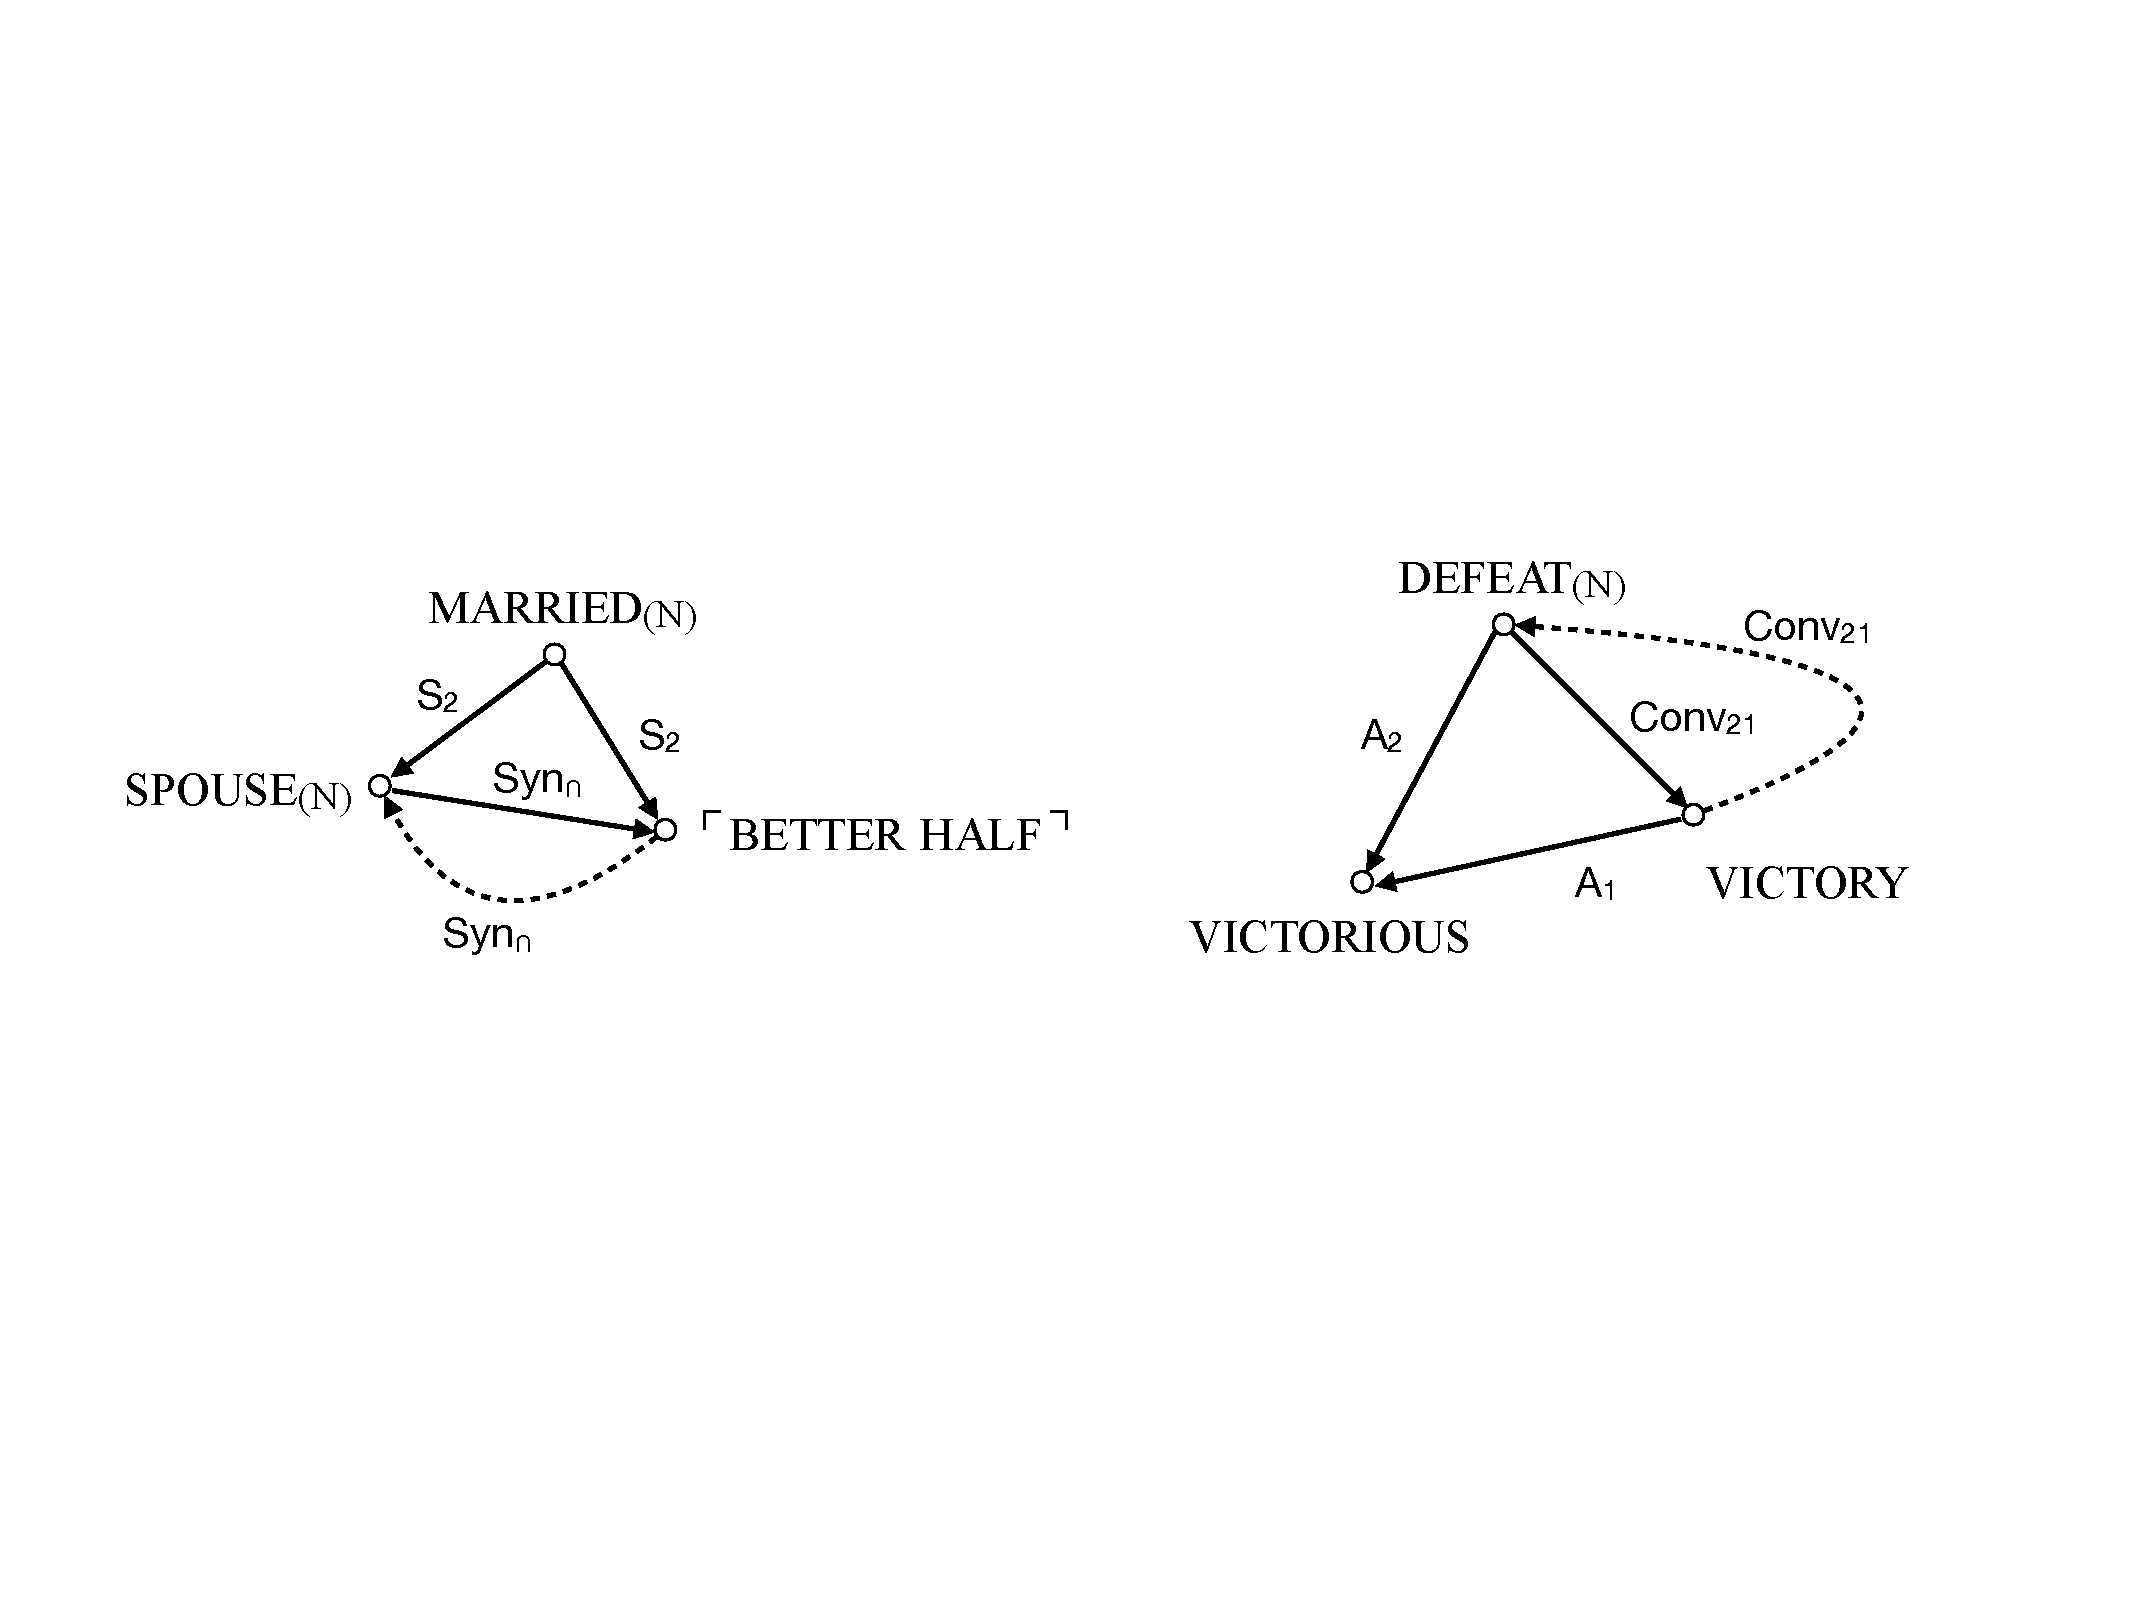
\includegraphics[width=0.9\linewidth]{Fig/LexicalNetworks/LFClusters.pdf}
\caption{Two LF-based lexical clusters}\label{fig:LFClusters}
\end{figure}

In \figref{fig:LFClusters}, solid arrows correspond to illustrations given in \ref{ex:clusteringInfRule1} and \ref{ex:clusteringInfRule2}; dashed arrows are additional clustering LF relations.

\subsubsection{Lexical vs. topological proximity}\label{sec:lexicalProximityTopologicalProximity}

Formal properties presented above show that $\mathcal{G}_{LS}$s are not \notion{random graphs}\index[notion]{graph!random \tld}\index[notion]{random graph}, i.e., graphs in which nodes and connecting arcs are randomly distributed.\footnote{In mathematical\slashs{}statistical terms, a random graph is a graph in which the distribution of node degrees follows a Poisson law; by contrast, the degree distribution of a small-world graph follows a power law \parencite[849]{Gaume2008}.} They are structured as small-world networks, whose topological properties can be exploited to access, study, and reason on the information they encode. The main advantage of small-world lexical networks over the better-known lexical taxonomies\index[notion]{taxonomy}\index[notion]{lexical network!taxonomic \tld} (\sectref{sec:shapeOfLexicons}, p.\thinspace\pageref{sec:shapeOfLexicons}) is that they do not adhere to one primary classifying\slashs{}hierarchization principle; consequently, they allow for very flexible and varied types of computation.

To illustrate the computability of small-world networks, we focus here on \notion{lexical proximity}\index[notion]{proximity, lexical} (whether semantic or combinatorial) that can be inferred from the topology of $\mathcal{G}_{LS}$s\index[notion]{graph!topology of a \tld}\index[notion]{topology}. This is well illustrated in visualizations\index[notion]{visualization} performed by the Spiderlex\index[notion]{Spiderlex} graph browser\index[notion]{network \lfgp{see also \textit{graph}}!\tld\ browser} (cf. \sectref{sec:LFRelationsBackboneOfLFs}, ``Visualization of Lexical Systems,'' p.\thinspace\pageref{rem:visualizationLS}), where clusters of lexical entities\index[notion]{cluster of nodes in a graph}\index[notion]{node of a network\slashs{}graph!cluster of \tlds} are identified by a stochastic algorithm that computes \notion{topological proximity}\index[notion]{topology!topological proximity} between lexical nodes \parencite{Gaume2004,Gaume2008}. This proximity is visually represented by two means: 

\begin{itemize}

\item the geometric distribution of nodes in the visualization\index[notion]{node of a network\slashs{}graph!geometric distribution of \tlds}\index[notion]{geometric distribution of graph nodes} -- the closer the nodes from the viewpoint of the graph topology, the closer they are positioned;

\item the color coding of node clusters identified by the topological analysis -- these clusters correspond to semantic-combinatorial classes of lexical entities.

\end{itemize}

\paragraph*{Lexical spaces.}\label{par:lexicalSpaces}

We have established earlier that $\mathcal{G}_{LS}$s possess a high clustering rate\index[notion]{cluster of nodes in a graph!clustering rate}\index[notion]{graph!clustering rate of a \tld} (\sectref{sec:basicsGraphTheory}, p.\thinspace\pageref{par:highClusteringRate}): at the microscopic level\index[notion]{microscopic structure (of a graph)}, their nodes tend to form small clusters of lexical entities that are mutually interrelated. Such clusters are of course identified by the topological analysis of a $\mathcal{G}_{LS}$. However, at the macroscopic level\index[notion]{macroscopic structure (of a graph)}\index[notion]{graph!microscopic vs. macroscopic structure of a \tld}, broader clusters are also identified; they bring together lexical entities that are more loosely related but form a distinct semantic-combinatorial \notion{lexical space}\index[notion]{lexical space} in the graph and, hopefully, in the Mental Lexicon\index[notion]{Mental Lexicon} this graph encodes.

\figref{fig:proxemyCIGARETTE}\phantomsection\label{txt:lexicalProximityCIGARETTE} below serves to illustrate the notion of lexical space and, more broadly, the outcome of a $\mathcal{G}_{LS}$'s topological analysis. It shows:

\begin{itemize}

\item lexical proximity identified by means of a topological analysis of the fr-LN\index[notion]{lexical network!French \tld\ [fr-LN]}\index[notion]{lexical database!French Lexical Network [fr-LN]};

\item visualization means used by Spiderlex to represent lexical spaces.

\end{itemize}

In this illustration, lexical proximity is  computed on the polysemy structure\index[notion]{polysemy!\tld\ structure of a vocable}\index[notion]{vocable!polysemy structure of a \tld} of the French vocable \textsc{cigarette}, which has been explained in \sectref{sec:non-LFRelationsInLSs} (p.\thinspace\pageref{txt:CIGARETTE}). To work on the complete polysemy of \textsc{cigarette}, three topological explorations are performed as so-called \textit{random walks} \parencite[Sec.~3]{Gaume2008}: one for each sense of the vocable taken as point of origine of the random walk. The three lexical nodes that are origines of random walks appear in \figref{fig:proxemyCIGARETTE} as triangles, rather than discs.

\begin{figure}

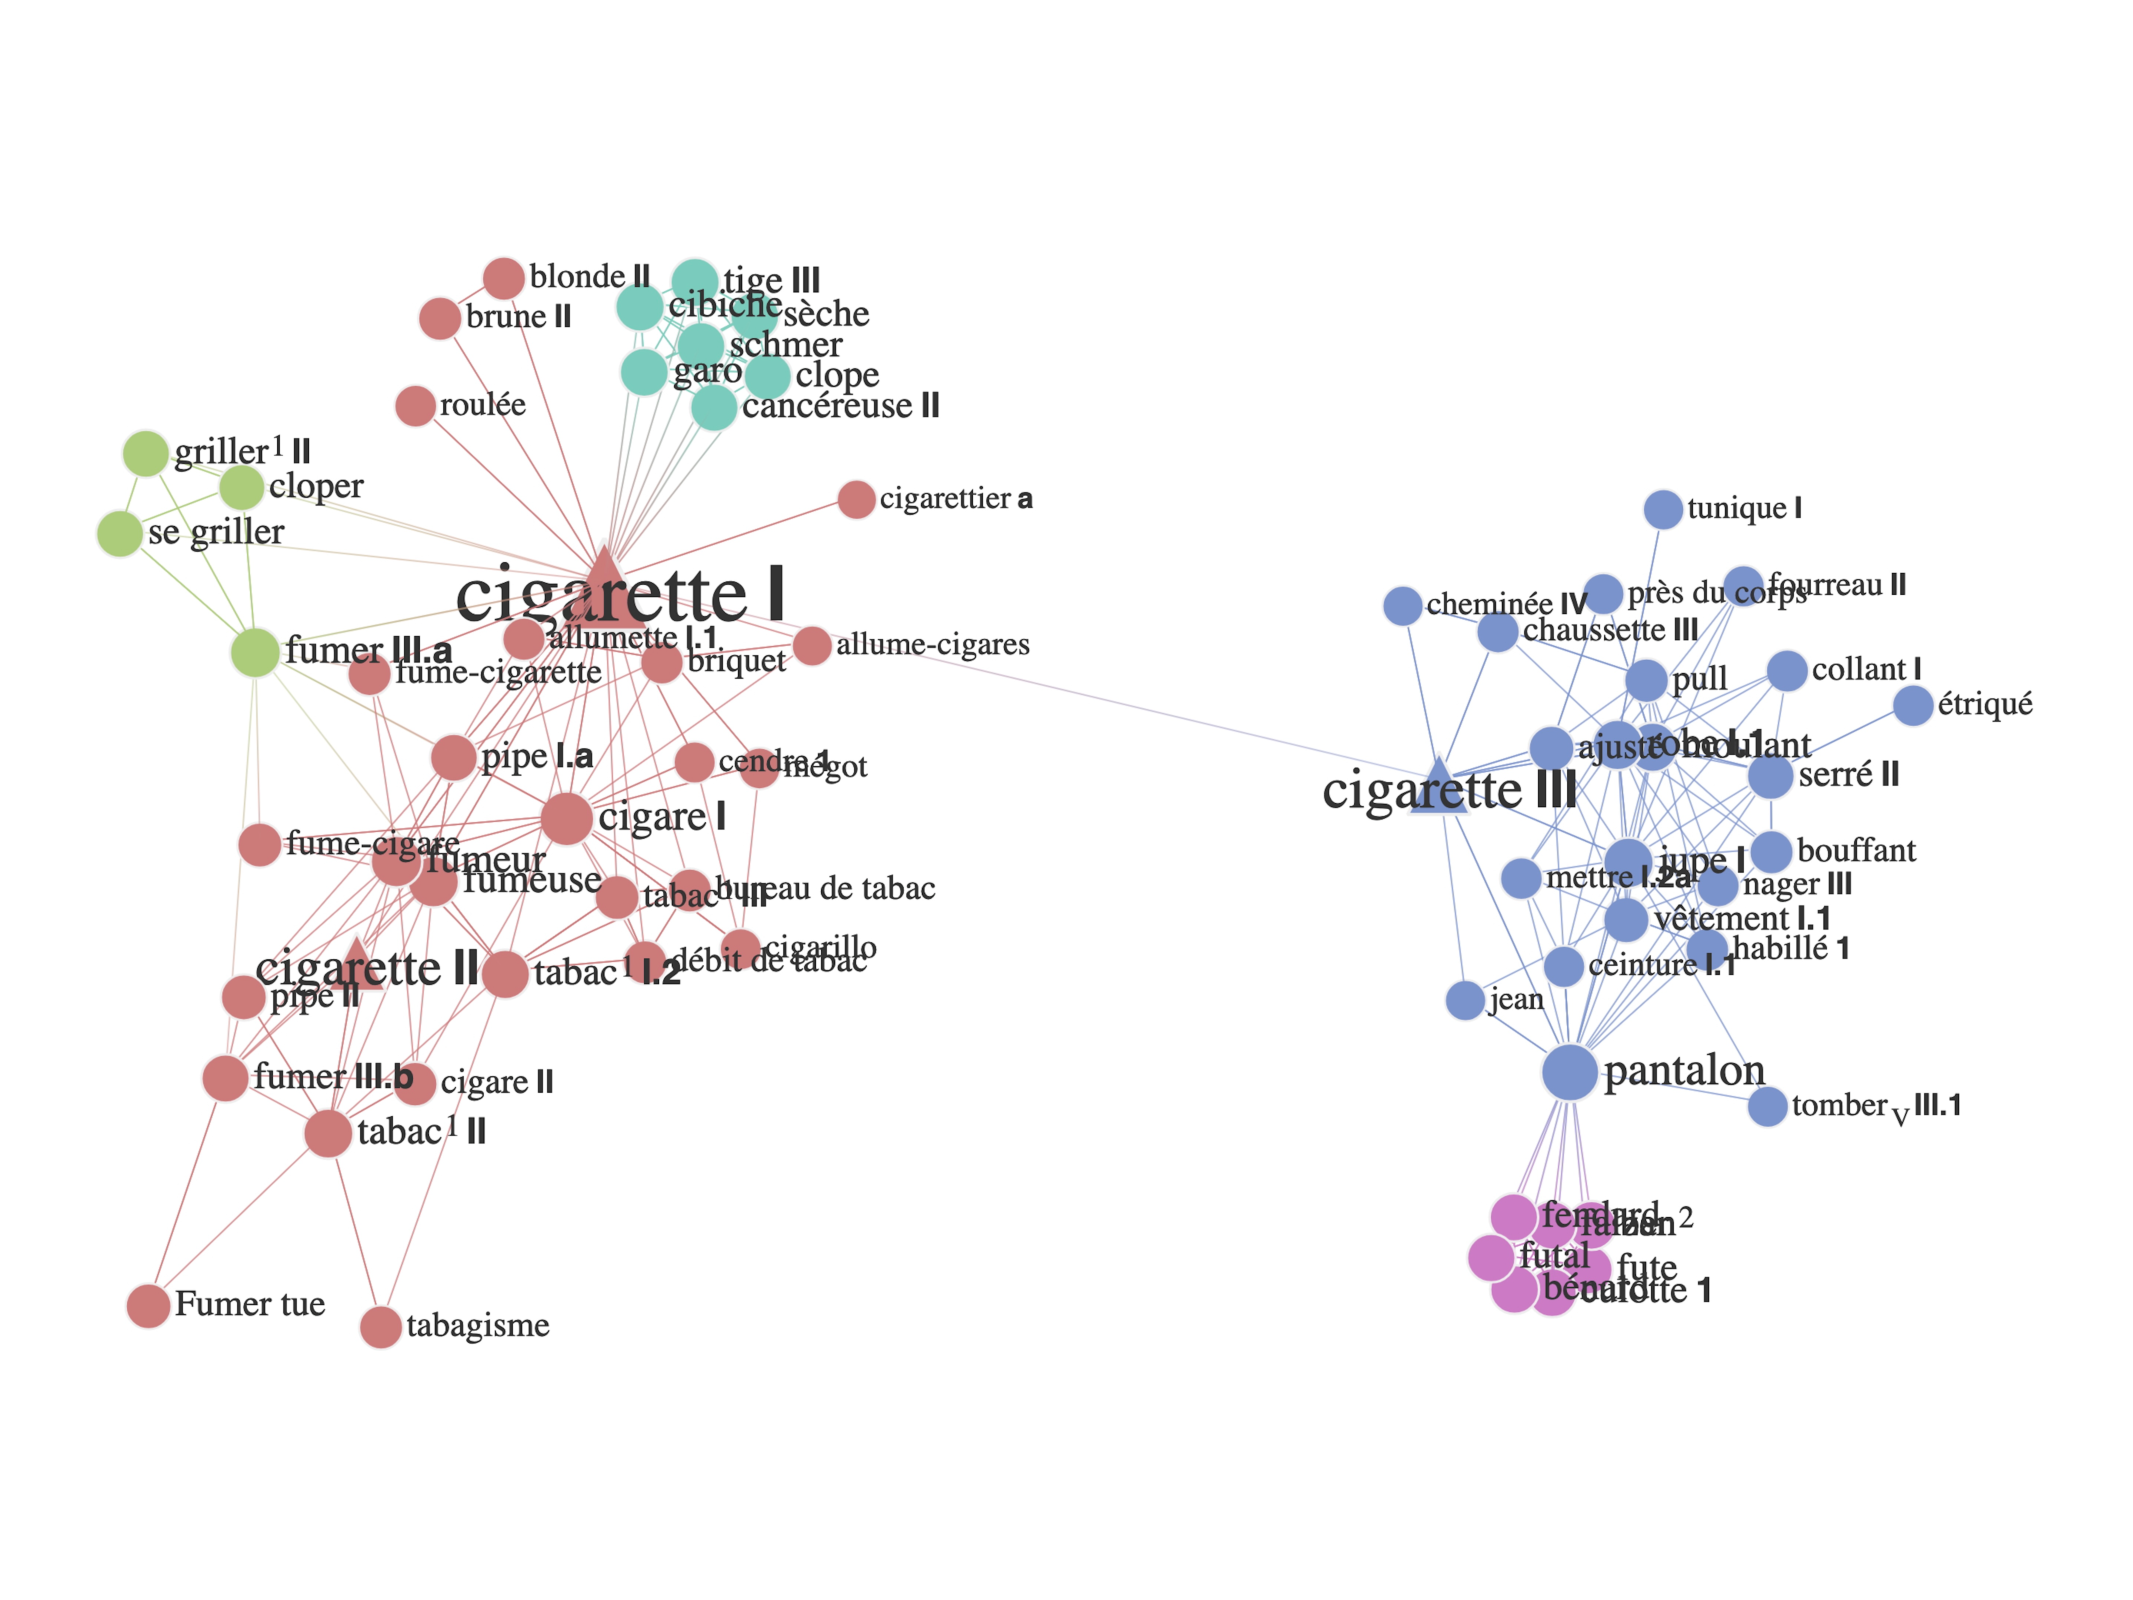
\includegraphics[width=\linewidth]{Fig/LexicalNetworks/proxemyCIGARETTE.pdf}
\caption{Lexical proximity computed on the polysemy of {\smaller French}~\textsc{cigarette} in the fr-LN}\label{fig:proxemyCIGARETTE}
\end{figure}

Let us make two comments on \figref{fig:proxemyCIGARETTE} in order to illustrate the linguistic relevance of the topological analysis and geometrization algorithms that have lead to this visualization.

First, the basic lexical unit\index[notion]{basic lexical unit of a vocable}\index[notion]{vocable!basic lexical unit of a \tld} \textsc{cigarette}\sensenum{I} and the metonymic\index[notion]{metonymy} sense \textsc{cigarette}\sensenum{II} `habit of smoking \textit{cigarettes}\sensenum{I}' form together a single lexical space, while the met\-aphoric\index[notion]{metaphor} sense \textsc{cigarette}\sensenum{III} `\lfgp{piece of clothing X} long and tight against the body, \idiom{as if} it had the shape of a \textit{cigarette}\sensenum{I}' is singled out, at the center of its own lexical space. These two spaces are located far apart, their connection holding by only one thread: the metaphor copolysemy\index[notion]{polysemy!co\tld}\index[notion]{copolysemy!\tld\ relation of metaphor} relation between \textsc{cigarette}\sensenum{I} and \textsc{cigarette}\sensenum{III}. This reflects the fact that a metonymy belongs to the same broad conceptual domain as its source, while a metaphor can totally escape the gravitation field, so to speak, of the copolyseme it originates from.

Second, the two lexical spaces identified above are themselves constituted of clusters that display their own lexical cohesion. Such is the case, in the lexical space of \textsc{cigarette}\sensenum{I} and \textsc{cigarette}\sensenum{II} combined, of the small cluster constituted of \textsc{fumer}\sensenum{III} `smoke\tsub{(V)}' -- that is \lfappl{Real\tsub{1}}{\textit{cigarette}\sensenum{I}} -- and three of its synonyms: \textsc{cloper}, \lu{griller}{}{1}{II} and \textsc{se~griller} (see top left corner of \figref{fig:proxemyCIGARETTE}). This is an extremely tight cluster -- and it is geometrically displayed as such -- for two linguistic reasons: (i)~the lexical units it contains are all values of \lf{Syn} for each other\footnote{Such cluster is called a \textit{clique}: a (sub)graph where every two nodes are connected.}\index[notion]{clique} and (ii)~they are additionally all values of the same LF application \lfappl{Real\tsub{1}}{\textit{cigarette}\sensenum{I}}.

\begin{furtherreading}
On the Lexical System approach to the modeling of polysemy, see \textcite{Polguere2018c}; on small-world lexical networks in lexicology\index[notion]{lexicology}\slashs{}lexicography\index[notion]{lexicography}, see \textcite{LoiseauEtAl2010,Polguere2014c-e,Polguere2016b-e}; in psycholinguistics\index[notion]{psycholinguistics}, see \textcite{GaumeEtAl2002,GaumeEtAl2008,DeDeyneEtAl2017}; in Natural Language Processing\index[notion]{Natural Language Processing}, see \textcite{Biemann2012}.
\end{furtherreading}

\section{Proof of concept: the French Lexical Network [fr-LN]}\label{sec:fr-LN}

In lieu of conclusion, we present briefly the lexicographic enterprise that produced the first large-scale Lexical System: the \notion{French Lexical Network} \mbox{[\notion{fr-LN}]}\index[notion]{French Lexical Network [fr-LN]|emph}\index[notion]{lexical database!French Lexical Network [fr-LN]|emph}\index[notion]{lexical network!French \tld\ [fr-LN]|emph}\index[notion]{lexical network!lexicography of \tlds}\index[notion]{lexicography!\tld\ of lexical networks}. Bibliographic references on important aspects of the fr-LN project are provided at the end of the section.

\subsection{Organization and progression of the fr-LN project}

The construction of the fr-LN is an ongoing long-term endeavor that started at the ATILF CNRS laboratory (Nancy, France) in 2011. An initial four-year funded project (called \textit{RELIEF}, see \cite{LuxPogodallaPolguere2011}) achieved the following tasks:

\begin{enumerate}

\item[1.a)] training of a team of lexicographers in the theory and practice of Explanatory Combinatorial Lexicology\slashs{}Lexicography\index[notion]{Explanatory Combinatorial!\tld\ Lexicology}\index[notion]{lexicology!Explanatory Combinatorial \tld}\index[notion]{Explanatory Combinatorial!computational \tld\ Lexicography}\index[notion]{lexicography!computational Explanatory Combinatorial \tld};

\item[1.b)] implementation -- in parallel with 1.a -- of a lexicographic editor\index[notion]{editor, lexicographic}\index[notion]{lexicography!lexicographic editor} tailor-made for the lexicography of Lexical Systems, whose capabilities were gradually incremented as the project proceeded with lexicographic description \parencite{GaderEtAl2012};

\item[2)] construction of a nucleus fr-LN for a core French vocabulary of around 3,700 vocables;

\item[3)] standard lexicographic work proceeding by important semantic fields (feelings, geographical elements, animals, ...).

\end{enumerate}

This initial stage of the project resulted in a Lexical System that modeled a significant sample of the French lexicon and that later expanded into a full-fledged small-world network\index[notion]{network \lfgp{see also \textit{graph}}!small-world \tld}\index[notion]{small-world!\tld\ network} (as defined in \sectref{sec:formalPropertiesLS}, p.\thinspace\pageref{sec:formalPropertiesLS}).

The fr-LN is in constant evolution both in terms of the number of lexical entities it describes and in terms of depth\slashs{}accuracy of the description. At the time of writing, its coverage can be quantified as follows:

\begin{center}
\setlength{\tabcolsep}{2.2pt}
%\setlength\extrarowheight{1.2pt}
\begin{tabular}{ l c r }

\textsf{\textbf{Lexical entities, i.e., network nodes}} & \textsf{\textbf{:}} & \textsf{\textbf{30,180}} \\
Vocables, i.e., lexicographic entries & : & 19,084 \\
Polysemy rate [= Lexical entities\slashs{}Vocables] & : & 1.58 \\[+6pt]

\textsf{\textbf{Lexical relations, i.e., network arcs}} & \textsf{\textbf{:}} & \textsf{\textbf{85,941}} \\
LF relations & : & 67,478 \\
Copolysemy relations & : & 9,960 \\
Idiom-component relations & : & 8,171 \\
Meaning-inclusion relations & : & 332 \\

\end{tabular}
\end{center}

The above statistics show that the current fr-LN is a lexical network of significant proportions: approximately 30,000 lexical nodes for 85,900 lexical relations. In accordance with the properties of Lexical Systems (cf. \sectref{sec:LFRelationsBackboneOfLFs}, p.\thinspace\pageref{sec:LFRelationsBackboneOfLFs}), LF relations form the bulk of the relational structure of the model. Meaning-inclusion relations are underrepresented as the work on the writing of lexicographic definitions is still at an embryonic stage.

In the absence of a dedicated lexicographic team, the fr-LN now evolves mainly on demand, according to the needs of researchers, language teachers, etc. who are collaborators on the project or are making use of the resource. The fr-LN's lexicographic data is available in open access, to be used for Natural Language Processing\index[notion]{Natural Language Processing} or computational linguistic work -- see \textcite{ATILF2024a}, for the network itself, and \textcite{ATILF2024b}, for the distribution of lexicographic examples\index[notion]{example, lexicographic} embedded in the fr-LN.

\subsection{New lexicography of lexical networks}\label{sec:lexicographyOfLNs}\index[notion]{lexicography!\tld\ of lexical networks|emph}\index[notion]{lexical network!lexicography of \tlds|emph}

The fr-LN project is mature enough -- in terms of coverage and applications it has generated -- to be seen as a proof of concept for Lexical Systems as plausible models of the Mental Lexicon. It demonstrates that network lexical models primarily structured by standard LF relations can offer new insights into the organization of lexical knowledge and, very importantly, that such models can indeed be lexicographically built.

As regards this last point, it is essential to stress the importance of the technological aspects of this new lexicography of lexical networks. Modern physics or astronomy could not exist without advanced technological means (cyclotrons, orbiting telescopes, etc.); similarly, though at a much more modest level, the lexicography of lexical networks has been made possible by the development of a sophisticated editor\index[notion]{editor, lexicographic}\index[notion]{lexicography!lexicographic editor} that allows lexicographers to literally jump from one lexical entity to another, encoding lexical relations while simultaneously creating new lexical nodes in the process, if the targeted lexical entity is not already present in the network.\footnote{We do not illustrate the use of the Lexical System lexicographic editor (named \textit{Dicet}, see \cite{GaderEtAl2012}) as a next generation editor (\textit{ItsyBitsy}) is under development at the time of writing.} This \emph{lexicographic gesture} \parencite{Polguere2012e-e} ensures that lexical entries always point to (the lexical entry of) actual lexical entities and forces lexicographers to encode a lexical relation as a link between two lexical entities that are (at least, minimally) modeled in the lexical network.

Anyone who has extensively used standard dictionaries (for language teaching, translation, etc.) knows that this is far from being the case in such models. The system of lexical relations present in a standard dictionary -- that has been termed the dictionary's \notion{mediostructure}\index[notion]{dictionary!mediostructure of a \tld}\index[notion]{mediostructure (of a dictionary)}\phantomsection\label{txt:mediostructure} \parencite{Wiegand1996,GouwsPrinsloo1998} -- is only modeled by cross-references in the text of the \notion{microstructure}\index[notion]{dictionary!microstructure of a \tld}\index[notion]{microstructure (of a dictionary)}. At the scale of the whole lexicon, however, this cross-referencing is necessarily approximate for logistic reasons. Only by building a lexical model that \emph{is}, so to speak, a mediostructure (i.e., a lexical network) can one ensure that the modeling of lexical relations -- the essence of the lexicon's structure (cf. Postulate~1, \sectref{sec:shapeOfLexicons}, p.\thinspace\pageref{txt:postulateStrucLexicons}) -- is truly valid and unambigous.

Finally, essential technology includes visualization and navigation tools such as Spiderlex\index[notion]{Spiderlex}\index[notion]{visualization} (extensively used to produce illustrations in the present chapter). Their purpose is threefold: improve access to the content of Lexical Systems, visualize complex topological information and help lexicographers diagnose missing or wrongly encoded information.

\begin{furtherreading}
On the strategy adopted to organize the fr-LN's initial growth based on the encoding of standard paradigmatic LF relations that are central in the system of LFs\index[notion]{lexical function!central \tld\ (in the system of standard \tlds)},\footnotemark\ see \textcite{LuxPogodallaPolguere2011} and \textcite{PolguereSikora2013a-e}; on the small-world structure of the fr-LN, see \textcite{GaderEtAl2014a-e}; on the implementation of analogical reasoning\index[notion]{analogical reasoning} in the fr-LN, see \textcite{Ollinger2014-e}; on lexicographic edition of Lexical Systems\index[notion]{editor, lexicographic}\index[notion]{lexicography!lexicographic editor}, see \textcite{GaderEtAl2012} and \textcite{Polguere2012e-e}; on the modeling of terminologies\index[notion]{terminology} within general language Lexical Systems, see \textcite{GotkovaEtAl2024}.
\end{furtherreading}\footnotetext{Roughly, those paradigmatic LFs whose ID is boxed in the table presenting the ``System of standard simple lexical functions'' (\chapref{chap:NotionLF}, p.\thinspace\pageref{tab:systFL}).}


\clearpage{\pagestyle{empty}\cleardoublepage}

% !TEX root = LF-IMAPol.tex

\ohead{Appendix: A sample lexical entry}

\chapter*{Appendix: A sample lexical entry}\label{chap:appendix1}
\addcontentsline{toc}{chapter}{Appendix: A sample lexical entry}

The lexical entry\index[notion]{lexical entry} of the noun \textsc{anger}\tsub{(N)} given below is intended to illustrate the use of lexical functions in lexicographic description\index[notion]{lexicography}. This is a reworked version of the entry presented in \textcite[Sec.~5, 42--46]{IordanskajaMelcuk2022}.
\vspace{20pt}

\noindent
{\Large \textsc{anger}\tsub{(N)}}{\large, noun, uncountable}

\subsubsection*{Definition}\index[notion]{definition!lexicographic \tld}\index[notion]{lexical entry!semantic zone of a \tld}\index[notion]{semantic!\tld\ zone of a lexical entry}\index[notion]{zone of a lexical entry!semantic \tld}\label{def:ANGER-n}

\begingroup
\small
%\renewcommand*{\arraystretch}{1.2}
\setlength{\tabcolsep}{2pt}
\begin{tabular}{ >{\raggedright\arraybackslash}p{2.8cm} c >{\raggedright\arraybackslash}p{8cm} }

\textit{X's anger at Y for Z}
& :
& X's unpleasant, unfavorable feeling directed at person Y and caused by Z -- such that \\

&
& \textbf{\textsf{Stimulus}} \\

&
& \setlength{\tabcolsep}{.5pt}\begin{tabular}{ p{0.35cm} >{\raggedright\arraybackslash}p{7cm} }
\SpecDiffIndent & X believes that Y is responsible for Z \\
\SpecDiffIndent & Z is undesirable for X \\
  \end{tabular} \\

&
& \textbf{\textsf{Effect}} \\

&
& \setlength{\tabcolsep}{.5pt}\begin{tabular}{ p{0.35cm} >{\raggedright\arraybackslash}p{7cm} }
\SpecDiffIndent & X wants to do something hostile to Y \weakcomp{in order to stop Z} \\
\SpecDiffIndent & X enters in a mental state such that X can easily lose self-control \\
  \end{tabular} \\

\end{tabular}
\endgroup

\subsubsection*{Government pattern}\index[notion]{government pattern}\index[notion]{lexical entry!cooccurence zone of a \tld}\index[notion]{zone of a lexical entry!cooccurrence \tld}\label{fig:governmentPatternANGER-n}

\begingroup
\small
\renewcommand*{\arraystretch}{1.1}
\begin{tabular}{ >{\raggedright\arraybackslash}p{3.3cm} >{\raggedright\arraybackslash}p{3.6cm} >{\raggedright\arraybackslash}p{3.6cm} }
\midrule

\multicolumn{1}{c}{`X'~$\Leftrightarrow$~\textsf{\textbf{I}}}
& \multicolumn{1}{c}{`Y'~$\Leftrightarrow$~\textsf{\textbf{II}}}
& \multicolumn{1}{c}{`Z'~$\Leftrightarrow$~\textsf{\textbf{III}}} \\

\midrule

{\footnotesize 1.} \syntRel{possess}\thinspace N's
& {\footnotesize 1.} \syntRel{obl-obj1}\thinspace \textit{against} N
& {\footnotesize 1.} \syntRel{obl-obj2}\thinspace \textit{for} N \\

{\footnotesize 2.} \syntRel{subj-adnom}\thinspace \textit{of} N
& {\footnotesize 2.} \syntRel{obl-obj1}\thinspace \textit{at} N
& {\footnotesize 2.} \syntRel{obl-obj2}\thinspace \textit{for} V\tsub{\textsc{ger}} \\

{\footnotesize 3.} \syntRel{modif}\thinspace \lfappl{A\tsub{0}}{N}
& {\footnotesize 3.} \syntRel{obl-obj1}\thinspace \textit{toward} N
& {\footnotesize 3.} \syntRel{obl-obj2}\thinspace \textit{over} N \\

&
& {\footnotesize 4.} \syntRel{obl-obj2}\thinspace \textit{over} V\tsub{\textsc{ger}} \\

\midrule
\end{tabular}
\endgroup

\noindent
\begingroup
\small
\renewcommand*{\arraystretch}{1.2}
\setlength{\tabcolsep}{4pt}
\begin{tabular}{ l >{\raggedright\arraybackslash}p{10cm} }

\multicolumn{2}{l}{\textbf{\textsf{Illustrations for the government pattern}}} \\

{\footnotesize \textsf{\textbf{I}}.1\thinspace+\thinspace\textsf{\textbf{II}}.1}
& \textit{Judy's} $\langle$\textit{Her}$\rangle$ \textit{anger against co-workers is not helpful.} \\

{\footnotesize \textsf{\textbf{I}}.1\thinspace+\thinspace\textsf{\textbf{II}}.2\thinspace+\thinspace\textsf{\textbf{III}}.2}
& \textit{They wanted to show their anger at the Government for signing the pact.} \\

{\footnotesize \textsf{\textbf{I}}.2\thinspace+\thinspace\textsf{\textbf{II}}.2\thinspace+\thinspace\textsf{\textbf{III}}.3}
& \textit{The anger of seniors at the Government over the health care reform will impact the elections.} \\

{\footnotesize\textsf{\textbf{II}}.3\thinspace+\thinspace\textsf{\textbf{III}}.2}
& \textit{She felt anger toward her parents for leaving her there.} \\

{\footnotesize\textsf{\textbf{I}}.3}
& \textit{Popular} \lfgp{= \lfappl{A\tsub{0}}{\textit{people}}} \textit{anger is rising.} \\

\end{tabular}
\endgroup

\subsubsection*{Lexical functions [LFs]}\label{sec:AppendixLFZone}

\begingroup
\small
%\renewcommand*{\arraystretch}{1.2}
\setlength{\tabcolsep}{3pt}
\begin{tabular}{ l c >{\raggedright\arraybackslash}p{7cm} }

\multicolumn{3}{l}{\textbf{Paradigmatic LFs}} \vspace{6pt}\\

\lf{Syn\tsub{$\supset$}} & : & \textit{fury}\textbf{;} \textit{indignation}\textbf{;} \textit{outrage}\textbf{;} \uslabel{formal}~\textit{wrath}\textbf{;} \uslabel{archaic}~\textit{ire} \\

\lf{Syn\tsub{$\cap$}} & : & \textit{rage} \\

\lf{Anti\tsub{$\cap$}} & : & \textit{gratefulness}\textbf{;} \textit{gratitude} \\

\lf{Gener} & : & \textit{feeling} \lfgp{\textit{of} \tld}\slashs\lfgp{\textit{angry}} \textit{feeling}\textbf{;} \textit{emotion} \lfgp{\textit{of} \tld}\slashs\lfgp{\textit{angry}} \textit{emotion} \\

\lf{Magn+Figur} & : & \textit{fire of} \tld\textbf{,} \textit{flame of} \tld\ \textbf{<} \textit{firestorm of} \tld \\

\lf{S\tsub{2}} & : & \textit{object}\textbf{,} \textit{subject}\textbf{,} \textit{target} \lfgp{\textit{of} \tld} \\

\lf{S\tsub{3}} & : & \textit{cause}\textbf{,} \textit{object}\textbf{,} \textit{subject} \lfgp{\textit{of} \tld}\textbf{,} \textit{reason} \lfgp{\textit{for} \tld} \\

\lf{A\tsub{1}} & : & \textit{angry}\textbf{,} \textit{in} \tld \\
\lf{Magn+A\tsub{1}} & : & \textit{filled} \textit{with} \tld\textbf{,} \textit{full of} \tld\ \textbf{<} \textit{consumed by} \tld\textbf{,} \uslabel{colloquial}~\idiom{\textit{blue in the face}}\textbf{,} \textit{fuming}\textbf{,} \uslabel{colloquial}~\idiom{\textit{hot under the collar}} \\

\lf{AntiVer+Magn+A\tsub{1}} & : & \textit{steamed-up} \senseex{I don't see why you got steamed-up about this slip of the
tongue.} \\

\lf{Able\tsub{1}} & : & \textit{irascible}\textbf{;} \textit{hot-tempered}\textbf{,} \textit{short-tempered}\textbf{;} \textit{short-fused} \\

\lf{PredAble\tsub{1}} & : & \idiom{\textit{be on a short fuse}}\textbf{,} \idiom{\textit{have a short fuse}} \\

\lf{Adv\tsub{1}} & : & \textit{angrily}\textbf{,} \textit{in} \tld\textbf{,} \textit{with} \tld \\

\lf{Sing}\label{txt:SingOfAnger} & : & \tld\ \textit{attack}\textbf{;} \textit{burst of} \tld\textbf{;} \textit{fit of} \tld\textbf{;} \textit{flash of} \tld\textbf{;} \textit{gust of} \tld\vspace{12pt} \\

\multicolumn{3}{l}{\textbf{Syntagmatic LFs}} \vspace{6pt}\\

\lf{Germ} & : & \textit{seeds} \lfgp{\textit{of} \tld} \\

\lf{Magn} & : & \textit{deep}\textbf{,} \textit{great} \textbf{<} \textit{fierce}\textbf{,} \textit{terrible} \textbf{<} \textit{extreme}\textbf{;} \textit{red} \textbf{<} \textit{black}\textbf{;} \textit{towering}\textbf{;} \textit{unbridled}\textbf{,} \textit{uncontrollable}\textbf{;} \textit{a\onewdf{}lot} \lfgp{\textit{of} \tld}\textbf{;} \idiom{\textit{over the top}} \lfconstr{anteposed}\textbf{;} \fused\textit{fury}\textbf{;} \fused\textit{rage} \\

\lf{Magn$_\text{1}^\text{quant}$} & : & \textit{widespread} \\

\lf{AntiMagn} & : & \textit{slight}\textbf{;} \idiom{\textit{a little bit}} \lfgp{\textit{of} \tld}\textbf{;} \fused\textit{annoyance} \\

\lf{IncepPredPlusMagn} & : & \idiom{\textit{builds up}}\textbf{,} \textit{grows}\textbf{,} \textit{mounts}\textbf{,} \textit{rises}\textbf{,} \idiom{\textit{swells up}}, \idiom{\textit{wells up}} \lfgp{\textit{inside} N\tsub{X}} \\

\lf{CausPredPlusMagn} & : & \textit{fuel}\textbf{,} \textit{stir} \lfgp{(\textsc{art}) \tld} \\

\lf{IncepPredMinusMagn} & : & \textit{cools}\textbf{,} \textit{fades}\textbf{,} \idiom{\textit{goes away}}\textbf{,} \textit{subsides} \\

\lf{CausPredMinusMagn} & : & \textit{calm}\textbf{,} \textit{soothe} \lfgp{\textsc{art} \tld} \\

\lf{Ver} & : & \textit{righteous} \\

\lf{Bon+Ver} & : & \textit{noble} \\

\lf{Oper\tsub{1}} & : & \textit{feel} \lfgp{(\textsc{art}) \tld} \\

\lf{IncepOper\tsub{1}} & : & \fused\uslabel{slang}~\idiom{\textit{have a cow}}\textbf{,} \fused\uslabel{slang}~\idiom{\textit{have kittens}} \\

\lf{Magn+Oper\tsub{1}} & : & \textit{blaze} \lfgp{\textit{with} \tld}\textbf{;} \textit{boil}\textbf{,} \textit{burst}\textbf{,} \textit{seethe} \lfgp{\textit{with} \tld} \\

\end{tabular}
\endgroup

\begingroup
\small
%\renewcommand*{\arraystretch}{1.2}
\setlength{\tabcolsep}{3pt}
\begin{tabular}{ l c >{\raggedright\arraybackslash}p{7cm} }

\lf{Magn+IncepOper\tsub{1}} & : & \textit{erupt} \lfgp{\textit{in} \tld}\textbf{,} \fused\idiom{\textit{blow up}} \lfgp{\textit{at} N\tsub{Y}}\textbf{,} \fused\uslabel{colloquial}~\idiom{\textit{blow a fuse}}\textbf{,} \fused\uslabel{colloquial}~\idiom{\textit{blow a gasket}}\textbf{,} \fused\uslabel{colloquial}~\idiom{\textit{blow} \lfgp{N\tsub{X}\textit{'s}} \textit{stack}}\textbf{,} \fused\uslabel{colloquial}~\idiom{\textit{blow} \lfgp{N\tsub{X}\textit{'s}} \textit{top}}\textbf{,} \fused\textit{explode}\textbf{,} \fused\uslabel{colloquial}~\idiom{\textit{fly off the handle}}\textbf{,} \fused\uslabel{colloquial}~\idiom{\textit{go ballistic}}\textbf{,} \fused\uslabel{colloquial}~\idiom{\textit{go through the roof}}\textbf{,} \fused\uslabel{colloquial}~\idiom{\textit{hit the ceiling}}\textbf{,} \fused\uslabel{colloquial}~\idiom{\textit{see red}} \\

\lf{CausOper\tsub{1}} & : & \fused\textit{anger}\tsub{(V)} \lfgp{N\tsub{X}} \\

\lf{IncepOper\tsub{2}} {\footnotesize or} \lf{Caus\tsub{2}Oper\tsub{2}} & : & \textit{attract}\textbf{,} \textit{draw} \lfgp{(\textsc{art}) \tld} \\

\lf{Caus\tsub{(2)}Func\tsub{0}} & : & \textit{provoke} \lfgp{(\textsc{art}) \tld}\textbf{;} \textit{arouse}\textbf{,} \textit{spark}\textbf{,} \textit{trigger} \lfgp{(\textsc{art}) \tld} \\

\lf{Caus\tsub{(2)}ContFunc\tsub{0}} & : & \textit{feed} \lfgp{\textsc{art} \tld} \\

\lf{Magn+Func\tsub{1}} & : & \textit{boils}\textbf{,} \textit{bubbles}\textbf{,} \textit{seethes} \lfgp{\textit{in} N\tsub{X}\slashs\textit{in} N\tsub{X}\textit{'s gut}\slashs\textit{in} N\tsub{X}\textit{'s soul}}\textbf{;} \textit{fills}\textbf{,} \textit{overcomes}\textbf{,} \textit{seizes} \lfgp{N\tsub{X}}\textbf{;} \textit{devours} \lfgp{N\tsub{X}} (\textit{from inside})\textbf{;} \fused\idiom{\textit{Smoke} $\langle$\textit{Steam}$\rangle$ \textit{is coming} $\langle$\textit{pouring}$\rangle$ \textit{out}} \lfgp{\textit{of} N\tsub{X}\textit{'s ears}} \\

\lf{Magn+IncepFunc\tsub{1}} & : & \textit{explodes} \lfgp{\textit{in} N\tsub{X}} \\

\lf{IncepFunc\tsub{2}} & : & \textit{falls} \lfgp{\textit{on} N\tsub{Y}} \\

\lf{Real\tsub{1,`hostile action'}} & : & \textit{vent} \lfgp{A\tsub{(poss)X} \tld\ \textit{on} N\tsub{Y}} \\[2pt]

\multicolumn{3}{>{\raggedright\arraybackslash}p{11cm}}{\leftskip=0.5cm{\footnotesize \remark{Note.}The semanteme configuration in subscript to the name of an LF identifies its target, i.e., the semantic component in the definition of the headword (in this case, \textsc{anger}\tsub{(N)}) on which bears the meaning of the LF (see \chapref{chap:NotionLF}, \sectref{sec:classeFLSyntagmatiques}, p.\thinspace\pageref{txt:targetOfSyntLF}).}} \\

\lf{AntiVerReal\tsub{1,`hostile action'}} & : & \idiom{\textit{take out}} \lfgp{A\tsub{(poss)X} \tld\ \textit{on} N\tsub{\textOmega}}\textbf{,} \fused\idiom{\textit{take it out}} \lfgp{\textit{on} N\tsub{\textOmega}} \lfconstr{\textOmega\ is not responsible for Z} \\

\lf{Adv\tsub{1}Real\tsub{1,`hostile action'}} & : & \idiom{\textit{out of}} \tld \\

\lf{SingS\tsub{0}Real\tsub{1,`hostile action'}} & : & \textit{outburst} \lfgp{\textit{of} \tld}\textbf{,} \lfgp{\textit{angry}} \textit{outburst} \\

\lf{Real\tsub{1,`loss of self-control'}} & : & \idiom{\textit{be beside oneself}} \lfgp{\textit{with} \tld} \\

\lf{Real\tsub{2,`hostile action'}} & : & \textit{endure} \lfgp{N\tsub{X}\textit{'s} \tld} \\

\lf{Fact\tsub{0,`loss of self-control'}} & : & \textit{explodes} \\

\lf{Perm\tsub{1}Fact\tsub{0}} & : & \idiom{\textit{give vent}} \lfgp{\textit{to} (\textsc{art}) \tld}\textbf{,} \idiom{\textit{let out}}\textbf{,} \textit{unleash}\textbf{,}\newline \textit{vent}\tsub{(V)} \lfgp{(\textsc{art})~\tld} \\

\lf{NonPerm\tsub{1}Fact\tsub{0}} & : & \textit{contain}\textbf{,} \textit{control}\textbf{,} \textit{stifle}\textbf{,} \textit{suppress} \lfgp{A\tsub{(poss)X}~\tld} \\

\lf{A\tsub{2}NonPerm\tsub{1}Fact\tsub{0}} & : & \textit{pent-up}\textbf{;} \textit{suppressed} \\

\lf{Fact\tsub{1,`loss of self-control'}} & : & \textit{blinds} \lfgp{N\tsub{X}} \\

\lfappl{Excess\tsup{motor}}{\textit{body}}---\lf{Sympt\tsub{13}} & : &
\lfgp{N\tsub{X}} \textit{is shaking} $\langle$\textit{trembling}$\rangle$ \lfgp{\textit{with} \tld} \\

\lfappl{Obstr}{\textit{breath}}---\lf{Sympt\tsub{13}} & : &
\lfgp{N\tsub{X}} \textit{is choking} \lfgp{\textit{of} \tld} \\

\lfappl{Excess\tsup{motor}}{\textit{brows}}---\lf{Sympt\tsub{123}} & : &
\lfgp{N\tsub{X}} \textit{furrows} \lfgp{A\tsub{(poss)X} \textit{brows} (\lfgp{\textit{in} \tld})} \\

\lfappl{Excess\tsup{express}}{\textit{eyes}}---\lf{Sympt\tsub{23}} & : &
\lfgp{N\tsub{X}\textit{'s eyes}} \textit{shine} \lfgp{\textit{with} \tld} \\

\lfappl{Excess\tsup{express}}{\textit{eyes}}---\lf{Sympt\tsub{1}} & : &
\fused\lfgp{N\tsub{X}} \idiom{\textit{looks daggers}} \lfgp{\textit{at} N\tsub{Y}} \\

\lfappl{Excess\tsup{express}}{\textit{eyes}}---\lf{Sympt\tsub{31}} & : &
\textit{seethes} \lfgp{\textit{in} N\tsub{X}\textit{'s eyes}} \\

\lfappl{Excess\tsup{motor}}{\textit{face}}---\lf{Sympt\tsub{1}} & : &
\fused\lfgp{N\tsub{X}} \textit{snarles} \lfgp{\textit{at} N\tsub{Y}} \\

\lfappl{Excess\tsup{color}}{\textit{face}}---\lf{Sympt\tsub{23}} & : &
\lfgp{N\tsub{X}\textit{'s face}} \textit{turns red} (\lfgp{\textit{with} \tld}) \\

\end{tabular}\index[notion]{target of an LF}\index[notion]{lexical function!target of a \tld}\index[notion]{headword of a lexical entry}\index[notion]{lexical entry!headword of a \tld}
\endgroup

\begingroup
\small
%\renewcommand*{\arraystretch}{1.2}
\setlength{\tabcolsep}{3pt}
\noindent
\begin{tabular}{ l c >{\raggedright\arraybackslash}p{7cm} }

\lfappl{Excess\tsup{color}}{\textit{face}}---\lf{Sympt\tsub{13}} & : &
\lfgp{N\tsub{X}} \textit{is flushed} $\langle$\textit{is red}$\rangle$ (\lfgp{\textit{with} \tld}) \\

\lfappl{Excess\tsup{motor}}{\textit{teeth}}---\lf{Sympt\tsub{123}} & : &
\lfgp{N\tsub{X}} \textit{grinds} \lfgp{A\tsub{(poss)X}} \textit{teeth} (\lfgp{\textit{in} \tld}) \\

\lfappl{Obstr\tsup{color}}{\textit{face}}---\lf{Sympt\tsub{23}} & : &
\lfgp{N\tsub{X}\textit{'s face}} \textit{blanches} \lfgp{\textit{with} \tld}\textbf{;} \lfgp{N\tsub{X}\textit{'s face}} \idiom{\textit{clouds over}} (\lfgp{\textit{with} \tld}) \\

\lfappl{Obstr\tsup{color}}{\textit{face}}---\lf{Sympt\tsub{13}} & : &
\lfgp{N\tsub{X}} \textit{is livid} \lfgp{\textit{with} \tld} \\

\lfappl{Excess\tsup{motor}}{\textit{feet}}---\lf{Sympt\tsub{123}} & : &
\lfgp{N\tsub{X}} \textit{stamps} $\langle$\textit{stomps}$\rangle$ \lfgp{A\tsub{(poss)X}} \textit{feet} \lfgp{\textit{in} \tld}\textbf{,} \fused\textit{thumps} \lfgp{A\tsub{(poss)X}} \textit{feet}  \\

\lfappl{Excess}{\textit{voice}}---\lf{Sympt\tsub{13}} & : &
\lfgp{N\tsub{X}} \textit{shouts} $\langle$\textit{yells}$\rangle$ \lfgp{\textit{in} \tld} \\

\end{tabular}
\endgroup

\subsubsection*{Examples}\index[notion]{example, lexicographic}

\begingroup
\small

Examples are extracted from the COCA corpus\index[notion]{COCA corpus} \parencite{Davies2008}.\medskip

\setcounter{ExNo}{0}

\ex. \textit{Our anger generally tells us a lot more about ourselves than about the object of our anger.}

\ex. \textit{Well, you're both anti-social misfits, filled with anger and rage.}

\ex. \textit{Henrik looks at him with anger and, in an act of aggressive sublimation, knocks off the lamp and books from his father's table.}

\ex. \textit{She came out publicly in a fit of anger when a fan harassed her online.}

%\ex. \textit{Everything appears to be normal and healthy, but inside the intimacies of family life, unbridled anger and abusive manipulation are alive and at work.}

\ex. \textit{Their stories are outrageous and heartbreaking and fuel my anger.}

\ex. \textit{This righteous anger was a relief; it masked his sense of shame.}

\ex. \textit{Suddenly my suppressed anger explodes. How could he ever do this to me?}

\ex. \textit{Even if protesters do not vent their anger at the troops, there are some who argue that any demonstrations will cause psychic wounds.}

\ex. \textit{She had to endure the anger of friends and neighbors who saw her as a threat to their jobs in the mining industry.}

\ex. \textit{Sam jumps up from the table, trembling with anger.}

\ex. \textit{He was almost always on the verge of outright shouting in anger during the show.}

\endgroup

\subsubsection*{Idiom}\label{sec:AppendixIdiom}

\noindent
\idiom{\textsc{anger management}}

%Anger and haste hinder good counsel

\clearpage{\pagestyle{empty}\cleardoublepage}




\backmatter
\phantomsection%this allows hyperlink in ToC to work
\ohead{References}
\printbibliography[heading=references]
\cleardoublepage

\phantomsection
\addcontentsline{toc}{chapter}{\lsIndexTitle}
\addcontentsline{toc}{section}{\lsNameIndexTitle}
\ohead{\lsNameIndexTitle}
\printindex
\cleardoublepage

%\phantomsection
%\addcontentsline{toc}{section}{\lsLanguageIndexTitle}
%\ohead{\lsLanguageIndexTitle}
%\printindex[lan]
%\cleardoublepage

%\phantomsection
%\addcontentsline{toc}{section}{\lsSubjectIndexTitle}
%\ohead{\lsSubjectIndexTitle}
%\printindex[sbj]


\phantomsection
\addcontentsline{toc}{section}{Index of notions}
\ohead{Index of notions}
\printindex[notion]
\cleardoublepage

\phantomsection
\addcontentsline{toc}{section}{Index of lexical functions}
\ohead{Index of lexical functions}
\printindex[lf]
\ohead{}

\end{document}
